% !TEX TS-program = latexmk
% !TEX encoding = UTF-8 Unicode

% This is a book in LaTeX 2e. 
% See below for various notes.  
% To compile the file, you need to use the following command line commands in Linux:  
%	pdflatex --shell-escape -synctex=1  -recorder algebra.tex
%	bibtex algebra  
%	makeindex -s notation.gst -o not.gls not.glo 
%	makeindex algebra    
%   sage algebra.sagetex.sage
% and repeat each of these many times.
\documentclass[ContainsChinese]{mckaybook}

\Title{Concrete Algebra}
\Subtitle{With a View Toward Abstract Algebra}
\Author{\texorpdfstring{Benjamin \scotsMc{}Kay}{Benjamin McKay}}
\Location{University College Cork}
\BibliographyFile{algebra}

\usepackage{standalone}
\usepackage{xstring}
\usepackage{amsmath}
\usepackage{mathrsfs}		% the \mathscr command for script fonts
\usepackage{mleftright}		% fixes problems with \left and \right
\usepackage{verbatim}		% For verbatim quotation of programming code.
\usepackage{asymptote}
\usepackage{siunitx}
%  longdiv.tex  v.1  (1994)  Donald Arseneau  
%
%  Work out and print integer long division problems.  Use:
%       \longdiv{numerator}{denominator}
%  The numerator and denominator (divisor and dividend) must be integers, and
%  the quotient is an integer too.  \longdiv leaves a remainder.
%  Use this in any type of TeX.

\newcount\gpten % (global) power-of-ten -- tells which digit we are doing
\countdef\rtot2 % running total -- remainder so far
\countdef\LDscratch4 % scratch

\def\longdiv#1#2{%
 \vtop{\normalbaselines \offinterlineskip
   \setbox\strutbox\hbox{\vrule height 2.1ex depth .5ex width0ex}%
   \def\showdig{$\underline{\the\LDscratch\strut}$\cr\the\rtot\strut\cr
       \noalign{\kern-.2ex}}%
   \global\rtot=#1\relax
   \count0=\rtot\divide\count0by#2\edef\quotient{\the\count0}%\show\quotient
   % make list macro out of digits in quotient:
   \def\temp##1{\ifx##1\temp\else \noexpand\dodig ##1\expandafter\temp\fi}%
   \edef\routine{\expandafter\temp\quotient\temp}%
   % process list to give power-of-ten:
   \def\dodig##1{\global\multiply\gpten by10 }\global\gpten=1 \routine
   % to display effect of one digit in quotient (zero ignored):
   \def\dodig##1{\global\divide\gpten by10
      \LDscratch =\gpten
      \multiply\LDscratch  by##1%
      \multiply\LDscratch  by#2%
      \global\advance\rtot-\LDscratch \relax
      \ifnum\LDscratch>0 \showdig \fi % must hide \cr in a macro to skip it
   }%
   \tabskip=0pt
   \halign{\hfil##\cr % \halign for entire division problem
     $\quotient$\strut\cr
     #2$\,\overline{\vphantom{\big)}%
     \hbox{\smash{\raise3.5\fontdimen8\textfont3\hbox{$\big)$}}}%
     \mkern2mu \the\rtot}$\cr\noalign{\kern-.2ex}
     \routine \cr % do each digit in quotient
}}}

\endinput % Demonstration below:

\noindent Here are some long division problems

\indent
\longdiv{12345}{13} \quad
\longdiv{123}{1234} \quad
\longdiv{31415926}{2} \quad
\longdiv{81}{3} \quad
\longdiv{1132}{99} \quad
\longdiv{86491}{94}
\bye

\usepackage{cool}
\usepackage{tikz}			% TiKZ graphics packages
\usetikzlibrary{%
arrows,
backgrounds,
calc,
decorations.pathmorphing,
fit,
intersections,
petri,
positioning,
through
}
\usepackage{pgfplots}
\pgfplotsset{compat=1.14}
\usepackage{tikz-3dplot}
\usepackage{stackengine}
\usepackage{tensor}
\usepackage{epigraph-keys}	% Handles epigraphs at the start of each chapter.
\usepackage{sagetex}
\vrefwarning
\usepackage{morewrites}
\usepackage{bookmark}% http://ctan.org/pkg/bookmark  

%%.....Mathematics Commands
\def\cprime{\('\)} 			% For Russian names

\newcommand*{\defeq}%		% for definitions, A \defeq B means A is defined to be B.
{\mathrel{\vcenter{\baselineskip0.5ex \lineskiplimit0pt
                     \hbox{\scriptsize.}\hbox{\scriptsize.}}}%
                     =}
% I don't like the default \Re and \Im for complex numbers.
\renewcommand{\Re}{\ensuremath{\operatorname{Re}}} 
\renewcommand{\Im}{\ensuremath{\operatorname{Im}}}

% Various sets
\newcommand*{\Z}[1]{\ensuremath{\mathbb{Z}^{#1}}}
\newcommand*{\N}[1]{\ensuremath{\mathbb{N}^{#1}}}
\newcommand*{\R}[1]{\ensuremath{\mathbb{R}^{#1}}}
\newcommand*{\Q}[1]{\ensuremath{\mathbb{Q}^{#1}}}
\newcommand*{\C}[1]{\ensuremath{\mathbb{C}^{#1}}}
\NewDocumentCommand\Zmod{sm}{\ensuremath{\mathbb{Z}\!/{\IfBooleanTF{#1}{\pr{#2}}{#2}}\mathbb{Z}}}

% Brackets
\newcommand*{\pr}[1]{\ensuremath{\left(#1\right)}}
\newcommand*{\curly}[1]{\ensuremath{\left\{#1\right\}}}
\newcommand*{\of}[1]{\ensuremath{\!\pr{#1}}}
\newcommand*{\equalquestion}{\stackrel{?}{=}}

% greatest common divisor
\renewcommand*{\gcd}[1]{\ensuremath{\operatorname{gcd}	\left\{{#1}\right\}}}
\newcommand*{\lcm}[1]{\ensuremath{\operatorname{lcm}\left\{{#1}\right\}}}

\usepackage{calc}

\newcommand{\longdivision}[2]{
    \settowidth{\dividendlength}{#1}
    \settowidth{\divisorlength}{#2}
    \settoheight{\dividendheight}{#1}
    \settoheight{\maxheight}{#1#2}
    \settoheight{\divisorheight}{#2}

    \begin{tikzpicture} [baseline=.5pt]
        \node at (-.5*\divisorlength-1pt,.5*\divisorheight) {#2};
        \node at (.5*\dividendlength+5pt,.5*\dividendheight) {#1};
        \draw [thick]  (0pt,-.22*\dividendheight) arc (-70:60:\maxheight*.41 and \maxheight*.82) -- ++(\dividendlength+7pt,0pt);
    \end{tikzpicture}
}

\newlength{\dividendlength}
\newlength{\divisorlength}
\newlength{\dividendheight}
\newlength{\divisorheight}
\newlength{\maxheight}

%% Two columns proofs:
% Usage:
%\begin{twocolumnproof}
%\pf{0}{0 + 0}[problem~1] \\
%\pf{a \cdot 0}{a \cdot (0 + 0)}[multiplying by \(a\)] \\
%\pf{a \cdot 0}{a \cdot 0 + a \cdot 0}[the distributive law] \\
%\pf{\text{Let } b}{-(a \cdot 0)} \\
%\pf{a \cdot 0 + b}{(a \cdot 0 + a \cdot 0) + b}[adding \(b\) to both sides] \\
%\pf{a \cdot 0 + b}{a \cdot 0 + (a \cdot 0 + b)}[the associative law for addition] \\
%\pf{0}{a \cdot 0 + 0}[the definition of \(b\)] \\
%\lastpf{0}{a \cdot 0}[the definition of \(0\)]
%\end{twocolumnproof}
\NewDocumentEnvironment{twocolumnproof}{}{\csname align*\endcsname}{\csname endalign*\endcsname}
\NewDocumentCommand\mainproofstep{mO{=}mom}{#1&#2#3\IfValueT{#4}{&{\quad}&\text{by #4}}#5}
\NewDocumentCommand\pf{mO{=}mo}{\mainproofstep{#1}[#2]{#3}[#4]{,}}
\NewDocumentCommand\lastpf{mO{=}mo}{\mainproofstep{#1}[#2]{#3}[#4]{.}}


\NewDocumentCommand\cardinality{sm}%
{%
\IfBooleanTF{#1}%
{\tensor[^{\#}]{(#2)}{}}%
{\tensor[^{\#}]{{#2}}{}}%
}%


% \congmod[p]{b}{c} means b=c (mod p).
\NewDocumentCommand\congmod{omm}{\IfValueTF{#1}{#2 \equiv #3 \pmod{#1}}{#2 \equiv #3}}

%\Proj[2]{k}
%or
%\Proj{2}
\NewDocumentCommand\Proj{om}{\IfValueTF{#1}{\mathbb{P}^{#1}\!\of{#2}}{\mathbb{P}^{#2}}}

\newcommand{\resultant}[2]{%
\ensuremath{\operatorname{res}_{#1,#2}}
}%

\newcommand{\discriminant}[1]{%
\ensuremath{\Delta_{#1}}
}%

\newcommand*{\tr}[1]{\operatorname{tr} #1}

\newcommand*{\degree}[1]{\operatorname{deg} #1}

\setstackgap{L}{.7\baselineskip}

\newcommand*{\multiplicity}[3]%\multiplicity{point}{curve}{curve}
{\ensuremath{#2#3_{#1}}}

\newcommand*{\order}[2]%\order{point}{curve}
{\ensuremath{{#2}_{#1}}}

\newcommand*{\intersectionnumber}[2]%\intersectionnumber{curve}{curve}
{\ensuremath{\deg{#1#2}}}

\NewDocumentCommand\Gal{mm}{\operatorname{Aut}{#2/#1}}

% quaternions
\newcommand*{\Quat}[1]{\ensuremath{\mathbb{H}^{#1}}}

% octonions
\newcommand*{\Oct}[1]{\ensuremath{\mathbb{O}^{#1}}}

\newcommand*{\ii}{\ensuremath{\iota}}

\NewDocumentCommand\Hessian{m}{\ensuremath{\det #1''}}


\begin{document}%
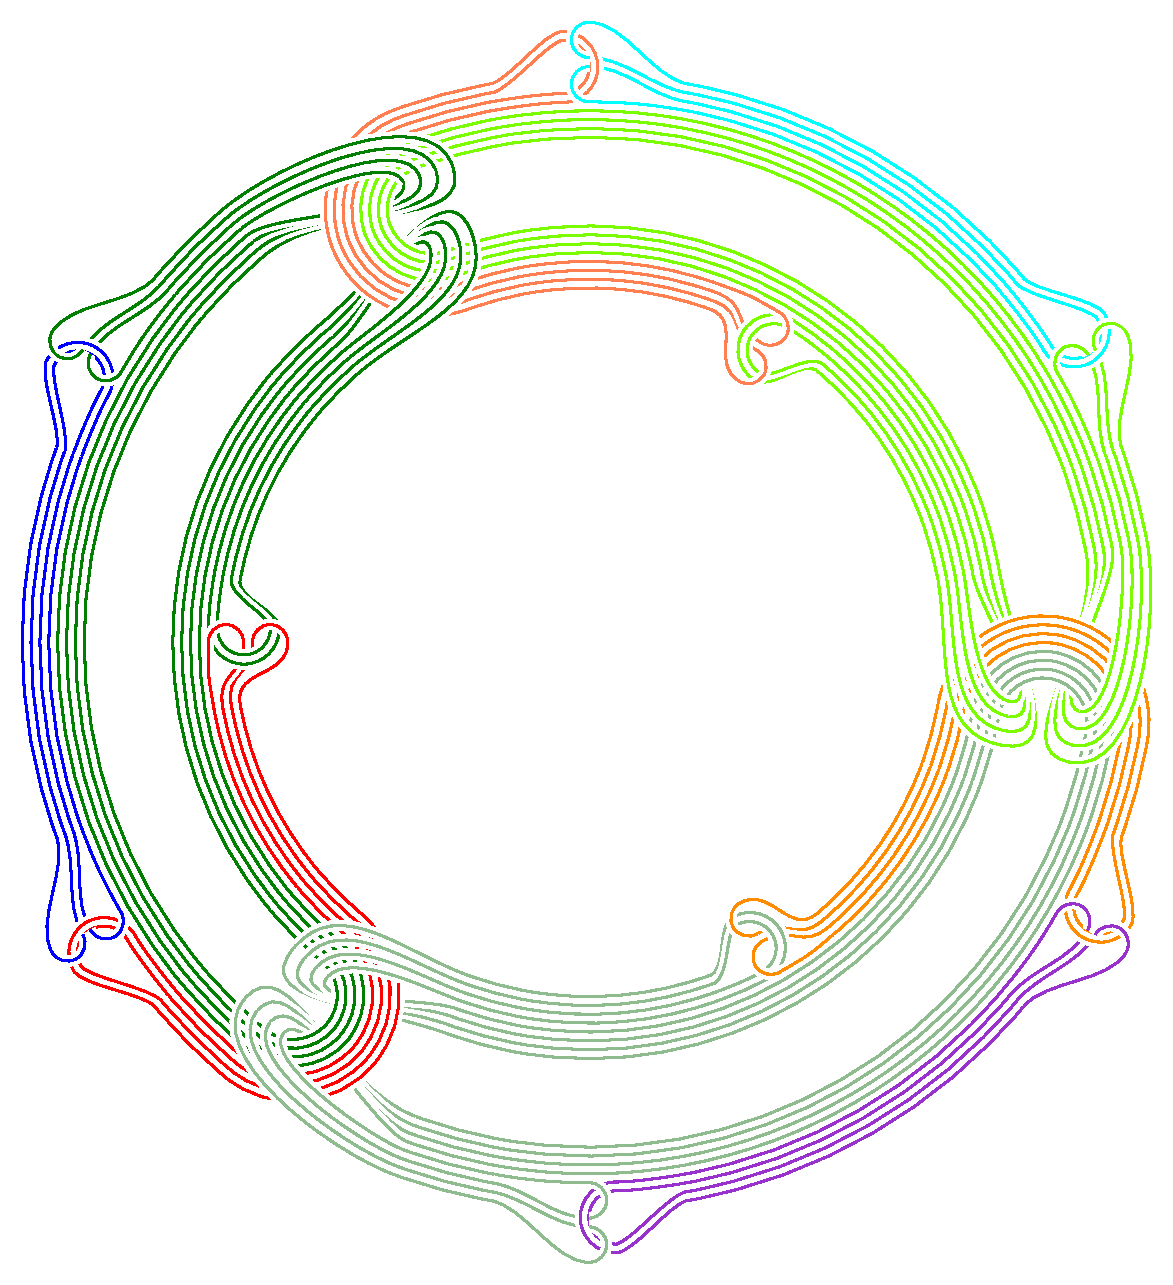
\includegraphics[width=.94\textwidth]{brunnian-ring.pdf}
\chapter*{Preface}
\epigraph[author={Ludwig Wittgenstein},source={Culture and Value}]{With my full philosophical rucksack I can only climb slowly up the mountain of mathematics.}\SubIndex{Wittgenstein, Ludwig}\SubIndex{Culture and Value}
These notes are from lectures given in 2015 at University College Cork.
They aim to explain the most concrete and fundamental aspects of algebra, in particular the algebra of the integers and of polynomial functions of a single variable, grounded by proofs using mathematical induction.
It is impossible to learn mathematics by reading a book like you would read a novel; you have to work through exercises and calculate out examples.
You should try all of the problems.
More importantly, since the purpose of this class is to give you a deeper feeling for elementary mathematics, rather than rushing into advanced mathematics, you should reflect about how the simple ideas in this book reshape your vision of algebra. 
Consider how you can use your new perspective on elementary mathematics to help you some day guide other students, especially children, with surer footing than the teachers who guided you.



\newpage

\newcommand{\quoteline}[1]{\rule[-.3\baselineskip]{0pt}{\baselineskip}--- #1}

\begin{epigraphs}\qitem[source={Applied Optics}, etc={vol. 11, A14, 1972}]
{The temperature of Heaven can be rather accurately computed.  Our authority is Isaiah 30:26, ``Moreover, the light of the Moon shall be as the light of the Sun and the light of the Sun shall be sevenfold, as the light of seven days.''  Thus Heaven receives from the Moon as much radiation as we do from the Sun, and in addition \(7 \times 7=49\) times as much as the Earth does from the Sun, or 50 times in all.  The light we receive from the Moon is one \(1/\num{10000}\) of the light we receive from the Sun, so we can ignore that\dots.  The radiation falling on Heaven will heat it to the point where the heat lost by radiation is just equal to the heat received by radiation, i.e., Heaven loses 50 times as much heat as the Earth by radiation.  Using the Stefan-Boltzmann law for radiation, \((H/E)\) temperature of the earth \((\sim\SI{300}{\kelvin})\), gives \(H\) as \(\SI{798}{\kelvin}\) \((\SI{525}{\celsius})\).  The exact temperature of Hell cannot be computed\dots.  [However] Revelations 21:8 says ``But the fearful, and unbelieving \dots shall have their part in the lake which burneth with fire and brimstone.''  A lake of molten brimstone means that its temperature must be at or below the boiling point, \(\SI{444.6}{\celsius}\).  We have, then, that Heaven, at \(\SI{525}{\celsius}\) is hotter than Hell at \(\SI{445}{\celsius}\).}\SubIndex{heaven}\SubIndex{hell}\SubIndex{optics}\SubIndex{temperature}\SubIndex{Applied Optics}
\qitem[author={Hermann Weyl},source={Invariants}, etc={Duke Mathematical Journal 5, 1939, 489--502}]{In these days the angel of topology and the devil of abstract algebra fight for the soul of every individual discipline of mathematics.}
\qitem[author={Goethe}, source={Faust}]{--- and so who are you, after all? \\
--- I am part of the power which forever wills evil and forever works good.}%
\SubIndex{Goethe, Johann Wolfgang von}\SubIndex{Faust}
\qitem[source={Quran}, etc={2:1/2:6-2:10 \emph{The Cow}}]{This Book is not to be doubted.}%
\SubIndex{Quran}\SubIndex{cow}\SubIndex{doubt}
\end{epigraphs}

\afterpreface
% The chapters
\chapter{The integers}\label{chapter:integers}
\epigraph[author={Leopold Kronecker}]{God made the integers; all else is the work of man.}\SubIndex{Kronecker, Leopold}
\section{Notation}
We will write numbers using notation like \(\num{1234567.12345}\), using a decimal point \({.}\) at the last integer digit, and using thin spaces to separate out every 3 digits before or after the decimal point.
You might prefer \(\num[group-separator={,},output-decimal-marker={\cdot}]{1234567.12345}\) or \(\num[group-separator={,}]{1234567.12345}\), which are also fine.
We reserve the \(\cdot\) symbol for multiplication, writing \(2 \cdot 3=6\) rather than \(2 \times 3 = 6\).

\section{The laws of integer arithmetic}
The integers are the numbers \(\dots, -2, -1, 0, 1, 2, \dots\).
Let us distill their essential properties, using only the concepts of addition and multiplication.
\smallskip
\begin{itemize}
\item[]\emph{Addition laws:}\define{addition laws}
\begin{enumerate}
\item The associative law:\define{associative law!addition} For any integers \(a, b, c\): \((a+b)+c=a+(b+c)\).
\item The identity law:\define{identity law!addition} There is an integer \(0\) so that for any integer \(a\): \(a+0=a\).
\item The existence of negatives:\define{existence of negatives} for any integer \(a\): there is an integer \(b\) (denoted by the symbol \(-a\)) so that \(a+b=0\).
\item The commutative law:\define{commutative law!addition} For any integers \(a, b\): \(a+b=b+a\).
\end{enumerate}
\smallskip
\item[]\emph{Multiplication laws:}\define{multiplication laws}
\begin{enumerate}
\item The associative law:\define{associative law!multiplication} For any integers \(a, b, c\): \((ab)c=a(bc)\).
\item The identity law:\define{identity law!multiplication} There is an integer \(1\) so that for any integer \(a\): \(a1=a\).
\item The zero divisors law: For any integers \(a,b\): if \(ab=0\) then \(a=0\) or \(b=0\).
\item The commutative law:\define{commutative law!multiplication} For any integers \(a, b\): \(ab=ba\).
\end{enumerate}
\smallskip
\item[]\emph{The distributive law:}\define{distributive law}
\begin{enumerate}
\item For any integers \(a, b, c\): \(a(b+c)=ab+ac\).
\end{enumerate}
\smallskip
\item[]\emph{Sign laws:}\define{sign laws} \smallskip \\ 
Certain integers are called \emph{positive}.\define{positive}
\begin{enumerate}
\item The succession law:\define{succession} An integer \(b\) is positive just when either \(b=1\) or \(b=c+1\) for a positive integer \(c\).
\item Determinacy of sign:\define{determinacy of sign} Every integer \(a\) has precisely one of the following properties: \(a\) is positive, \(a=0\), or \(-a\) is positive.
\end{enumerate}
We write \(a<b\) to mean that there is a positive integer \(c\) so that \(b=a+c\). 
\smallskip
\item[]\emph{The law of well ordering:}\define{law of well ordering}\define{well ordering}
\begin{enumerate}
\item
Any nonempty collection of positive integers has a least element; that is to say, an element \(a\) so that every element \(b\) satisfies \(a<b\) or \(a=b\).
\end{enumerate}
\end{itemize}
\smallskip\noindent{}All of the other arithmetic laws we are familiar with can be derived from these.
For example, the associative law for addition, applied twice, shows that \((a+b)+(c+d)=a+(b+(c+d))\), and so on, so that we can add up any finite sequence of integers, in any order, and get the same result, which we write in this case as \(a+b+c+d\).
A similar story holds for multiplication.

Of course, we write \(1+1\) as \(2\), and \(1+1+1\) as \(3\) and so on.
Write \(a>b\) to mean \(b<a\).
Write \(a\le b\) to mean \(a<b\) or \(a=b\). 
Write \(a\ge b\) to mean \(b \le a\).
Write \(|a|\)\define{absolute value} to mean \(a\), if \(a \ge 0\), and to mean \(-a\) otherwise, and call it the \emph{absolute value}\define{absolute value} of \(a\).
An integer \(a\) is \emph{negative}\define{negative} if \(-a\) is positive.

\vspace{2cm}

To understand mathematics, you have to solve a large number of problems.
\epigraph[author={Frederick Douglass, statesman and escaped slave}]{I prayed for twenty years but received no answer until I prayed with my legs.}\SubIndex{Douglass, Frederick}
\begin{problem}{integers:use.laws}
For each equation below, what law above justifies it?
\begin{enumerate}
\item \(7(3+1)=7 \cdot 3 + 7 \cdot 1\)
\item \(4(9 \cdot 2)=(4 \cdot 9)2\)
\item \(2 \cdot 3=3 \cdot 2\)
\end{enumerate}
\end{problem}
\begin{answer}{integers:use.laws}
\begin{enumerate}
\item distributive
\item associative multiplication
\item commutative multiplication
\end{enumerate}
\end{answer}
\begin{problem}{integers:right.distrib}
Use the laws above to prove that for any integers \(a, b, c\): \((a+b)c=ac+bc\).
\end{problem}
\begin{answer}{integers:right.distrib}
By the commutative law of multiplication, \((a+b)c=c(a+b)\).
By the distributive law, \(c(a+b)=ca+cb\).
By two applications of the commutative law, \(ca+cb=ac+cb=ac+bc\).
\end{answer}
\begin{problem}{integers:zero.plus.zero}
Use the laws above to prove that \(0+0=0\).
\end{problem}
\begin{answer}{integers:zero.plus.zero}
For any integer \(a\): \(a+0=a\). Pick \(a\) to be \(a=0\).
\end{answer}
\begin{problem}{integers:zero.times.zero}
Use the laws above to prove that \(0 \cdot 0=0\).
\end{problem}
\begin{answer}{integers:zero.times.zero}
\begin{twocolumnproof}
\pf{0}{0 + 0}[problem \ref{problem:integers:zero.plus.zero}] \\
\pf{0 \cdot 0}{0 \cdot (0 + 0)}[multiplying by \(0\)] \\
\pf{0 \cdot 0}{0 \cdot 0 + 0 \cdot 0}[the distributive law] \\
\pf{\text{Let } b}{-(0 \cdot 0)} \\
\pf{0 \cdot 0 + b}{(0 \cdot 0 + 0 \cdot 0) + b}[adding \(b\) to both sides] \\
\pf{0 \cdot 0 + b}{0 \cdot 0 + (0 \cdot 0 + b)}[the associative law for addition] \\
\pf{0}{0 \cdot 0 + 0}[the definition of \(b\)] \\
\lastpf{0}{0 \cdot 0}[the definition of \(0\)] \\
\end{twocolumnproof}
\end{answer}
\begin{problem}{integers:any.times.zero}
Use the laws above to prove that, for any integer \(a\): \(a \cdot 0=0\).
\end{problem}
\begin{answer}{integers:any.times.zero}
\begin{twocolumnproof}
\pf{0}{0 + 0}[problem \ref{problem:integers:zero.plus.zero}] \\
\pf{a \cdot 0}{a \cdot (0 + 0)}[multiplying by \(a\)] \\
\pf{a \cdot 0}{a \cdot 0 + a \cdot 0}[the distributive law] \\
\pf{\text{Let } b}{-(a \cdot 0)} \\
\pf{a \cdot 0 + b}{(a \cdot 0 + a \cdot 0) + b}[adding \(b\) to both sides] \\
\pf{a \cdot 0 + b}{a \cdot 0 + (a \cdot 0 + b)}[the associative law for addition] \\
\pf{0}{a \cdot 0 + 0}[the definition of \(b\)] \\
\lastpf{0}{a \cdot 0}[the definition of \(0\)]
\end{twocolumnproof}
\end{answer}
\begin{problem}{integers:unique.minus}
Use the laws above to prove that, for any integer \(a\): there is exactly one integer \(b\) so that \(a+b=0\); of course, we call this \(b\) by the name \(-a\).
\end{problem}
\begin{answer}{integers:unique.minus}
There is at least one such \(b\), by the existence of negatives.
Suppose that \(a+b=0\) and that \(a+c=0\).
\begin{twocolumnproof}
\pf{(a+b)+c}{0+c} \\
\pf{}{c+0}[commutativity of addition] \\
\pf{}{c}[the definition of \(0\)] \\
\pf{}{(a+b)+c}[returning to the start again] \\
\pf{}{a+(b+c)}[associativity of addition] \\
\pf{}{a+(c+b)}[commutativity of addition] \\
\pf{}{(a+c)+b}[associativity of addition] \\
\pf{}{0+b}[the definition of \(c\)] \\
\pf{}{b+0}[commutativity of addition] \\
\lastpf{}{b}[the definition of \(0\)]
\end{twocolumnproof}
Hence \(b=c\).
\end{answer}
\begin{problem}{integers:minus.one.times}
Use the laws above to prove that, for any integer \(a\): \((-1)a=-a\).
\end{problem}
\begin{answer}{integers:minus.one.times}
\begin{twocolumnproof}
\pf{a+(-1)a}{a+a(-1)}[commutativity of multiplication] \\
\pf{}{a(1+(-1))}[the distributive law on the right hand side] \\
\pf{}{a(0)}[the definition of \(-\)] \\
\lastpf{}{0}[the definition of \(0\)] 
\end{twocolumnproof}
So \((-1)a\) fits the definition of \(-a\).
By problem~\vref{problem:integers:unique.minus}, \((-1)a=-a\).
\end{answer}
\begin{problem}{integers:min.min}
Use the laws above to prove that \((-1)(-1)=1\).
\end{problem}
\begin{answer}{integers:min.min}
By problem~\vref{problem:integers:minus.one.times}, \((-1)(-1)=-(-1)\) is the unique integer which, added to \(-1\), gives zero, and we know that this integer is \(1\).
\end{answer}
\begin{problem}{integers:abs.product}
Use the laws above to prove that, for any integers \(b,c\): \(|bc|=|b||c|\).
\end{problem}
\begin{problem}{integer:unique.zero}
Our laws ensure that there is an integer \(0\) so that \(a+0=0+a=a\) for any integer \(a\).
Could there be two different integers, say \(p\) and \(q\), so that \(a+p=p+a=a\) for any integer \(a\), and also so that \(a+q=q+a=a\) for any integer \(a\)?
(Roughly speaking, we are asking if there is more than one integer which can ``play the role'' of zero.)
\end{problem}
\begin{problem}{integer:unique.one}
Our laws ensure that there is an integer \(1\) so that \(a \cdot 1=1 \cdot a=a\) for any integer \(a\).
Could there be two different integers, say \(p\) and \(q\), so that \(ap=pa=a\) for any integer \(a\), and also so that \(aq=qa=a\) for any integer \(a\)?
\end{problem}
\begin{theorem}[The equality cancellation law for addition\define{equality cancellation law!addition}]
Suppose that \(a, b\) and \(c\) are integers and that \(a+c=b+c\).
Then \(a=b\).
\end{theorem}
\begin{proof}
By the existence of negatives, there is a integer \(-c\) so that \(c+(-c)=0\).
Clearly \((a+c)+(-c)=(b+c)+(-c)\).
Apply the associative law for addition: \(a+(c+(-c))=b+(c+(-c))\), so \(a+0=b+0\), so \(a=b\). 
\end{proof}
\begin{problem}{integers:m.b.p.c}
Prove that \(-(b+c)=(-b)+(-c)\) for any integers \(b,c\).
\end{problem}
\begin{answer}{integers:m.b.p.c}
We need to see that \((-b)+(-c)\) has the defining property of \(-(b+c)\): adding to \(b+c\) to give zero.
\begin{twocolumnproof}
\pf{(b+c)+((-b)+(-c))}{b+c+(-b)+(-c)}[as above: parentheses not needed] \\
\pf{}{b+(-b)+c+(-c)}[commutativity of addition] \\
\pf{}{0+0}[existence of negatives] \\
\lastpf{}{0}[the definition of \(0\)]
\end{twocolumnproof}
\end{answer}
\begin{problem}{integers:unique.predecessor}
A \emph{predecessor}\define{predecessor} of an integer \(b\) is an integer \(c\) so that \(b=c+1\).
Prove that every integer has a unique predecessor.
\end{problem}
\begin{answer}{integers:unique.predecessor}
If \(b=c+1=d+1\) for two integers \(c,d\), then \(c+1=d+1\) so \((c+1)+(-1)=(d+1)+(-1)\), where the existence of negatives ensures that there is a negative \(-1\) of \(1\).
So \(c+(1+(-1))=d+(1+(-1))\) by the associative law for addition.
So \(c+0=d+0\), by the existence of negatives law.
So \(c=d\), by the identity law for addition.
\end{answer}
We haven't mentioned subtraction\define{subtraction} yet.
\begin{problem}{integers:define.subtraction}
Suppose that \(a\) and \(b\) are integers.
Prove that there is a unique integer \(c\) so that \(a=b+c\).
Of course, from now on we write this integer \(c\) as \(a-b\).
\end{problem}
\begin{problem}{integers:minus.and.subtraction}
Prove that, for any integers \(a,b\), \(a-b=a+(-b)\).
\end{problem}

\begin{problem}{integers:subtraction.distributive}
Prove that subtraction \emph{distributes over multiplication}: for any integers \(a,b,c\), \(a(b-c)=ab-ac\).
\end{problem}

\begin{problem}{integers:define.subtraction.order}
Prove that any two integers \(b\) and \(c\) satisfy just precisely one of the conditions \(b>c\), \(b=c\), \(b<c\).
\end{problem}
\begin{theorem} The equality cancellation law for multiplication:\define{equality cancellation law!multiplication} for an integers \(a,b,c\) if \(ab=ac\) and \(a\ne 0\) then \(b=c\).
\end{theorem}
\begin{proof}
If \(ab=ac\) then \(ab-ac=ac-ac=0\).
But \(ab-ac=a(b-c)\) by the distributive law.
So \(a(b-c)=0\). By the zero divisors law, \(a=0\) or \(b=c\).
\end{proof}
\begin{problem}{integers:two.by.two}
We know how to add and multiply \(2 \times 2\) matrices with integer entries.
Of the various laws of addition and multiplication and signs for integers, which hold true also for such matrices?
\end{problem}
\begin{problem}{integers:successor}
Use the laws above to prove that the sum of any two positive integers is positive.
\end{problem}
\begin{answer}{integers:successor}
Suppose that there are positive integers \(b,c\) with \(b+c\) not positive.
By the law of well ordering, there is a least possible choice of \(b\), and, for that given \(b\), a least possible choice of \(c\).
If \(b=1\) then \(b+c=1+c=c+1\) is positive by the succession law.
If \(b \ne 1\), then \(b=d+1\) for some positive \(d\) by the succession law, and then \(b+c=(d+1)+c=(d+c)+1\).
This is not positive, so by the succession law, \(d+c\) is not positive.
But then \(d\) is smaller than \(b\), so \(b\) is not the least possible choice.
\end{answer}
\begin{problem}{integers:pos.times.pos}
Use the laws above to prove that the product of any two positive integers is positive.
\end{problem}
\begin{answer}{integers:successor}
Suppose that there are positive integers \(b,c\) with \(bc\) not positive.
By the law of well ordering, there is a least possible choice of \(b\), and, for that given \(b\), a least possible choice of \(c\).
If \(b=1\) then \(bc=c\) is positive.
If \(b \ne 1\), then \(b=d+1\) for some positive \(d\) by the succession law, and then \(bc=(d+1)c=dc+c\).
This is not positive, so by problem~\vref{problem:integers:successor}, \(dc\) is not positive.
But then \(d\) is smaller than \(b\), so \(b\) is not the least possible choice.
\end{answer}
\begin{problem}{integers:pos.product}
Use the laws above to prove that the product of any two integers is positive just when (1) both are positive or (2) both are negative.
\end{problem}
\begin{answer}{integers:pos.product}
If \(b,c >0\) or if \(b,c < 0\), we know that \(bc>0\).
If \(b>0\) and \(c<0\), say \(c=-d\) with \(d>0\), then \(bc=b(-d\).
If we add \(bd+b(-d))=b(d+(-d))=b0=0\).
So \(b(-d)=-(bd)\) is negative.
Similarly, if \(b<0\) and \(c>0\), \(bc=cb\) is negative.
\end{answer}
\begin{problem}{integers:neg.times.neg}
Use the laws above to prove that the product of any two negative integers is positive.
\end{problem}
\begin{problem}{integers:cancel.plus}
Prove the inequality cancellation law for addition:\define{inequality cancellation law!addition} For any integers \(a, b, c\): if \(a+c<b+c\) then \(a<b\).
\end{problem}
\begin{answer}{integers:cancel.plus}
\begin{twocolumnproof}
\pf{(b+c)-(a+c)}{b+c+(-(a+c))}[\(d-e=d+(-e)\) as above] \\
\pf{}{b+c+(-a)+(-c)}[\(-(d+e)=(-d)+(-e)\) as above] \\
\pf{}{b+c+(-c)+(-a)}[commutativity of addition] \\
\pf{}{b+0+(-a)}[existence of negatives] \\
\pf{}{b+(-a)}[definition of zero] \\
\lastpf{}{b-a}[\(d+(-e)=d-e\) as above]
\end{twocolumnproof}
So \(a+c < b+c\) just when \(a<b\).
\end{answer}
\begin{problem}{integers:cancel.times}
Prove the inequality cancellation law for multiplication:\define{inequality cancellation law!multiplication} For any integers \(a, b, c\): if \(a<b\) and if \(0<c\) then \(ac<bc\).
\end{problem}
\begin{answer}{integers:cancel.times}
By distributivity of subtraction, proven in problem~\vref{problem:integers:subtraction.distributive}, \(bc-ac=(b-c)a\).
Apply the solution of problem~\vref{problem:integers:pos.product}.
\end{answer}
\begin{problem}{integers:bounded}
Suppose that \(S\) is a set of integers.
A \emph{lower bound}\define{lower bound} on \(S\) is an integer \(b\) so that \(b\le c\) for every integer \(c\) from \(S\); if \(S\) has a lower bound, \(S\) is \emph{bounded from below}.\define{bounded from below}
Prove that a nonempty set of integers bounded from below contains a least element.
\end{problem}

\section{Division of integers}
\epigraph[author={Lewis Carroll}, source={Through the Looking Glass}]{Can you do Division?  Divide a loaf by a knife---what's the answer to that?}\SubIndex{Carroll, Lewis}\SubIndex{Through the Looking Glass}
We haven't mentioned division\define{division} yet.
\emph{Danger:} although \(2\) and \(3\) are integers, 
\[
\frac{3}{2}=1.5
\]
is \emph{not} an integer.
\begin{problem}{integers:define.division}
Suppose that \(a\) and \(b\) are integers and that \(b \ne 0\).
Prove from the laws above that there is \emph{at most} one integer \(c\) so that \(a=bc\).
Of course, from now on we write this integer \(c\) as \(\frac{a}{b}\) or \(a/b\).
\end{problem}
\begin{problem}{integers:division.by.zero}
\emph{Danger:} why \emph{can't} we divide by zero\SubIndex{division!by zero}?
\end{problem}
\begin{answer}{integers:division.by.zero}
Dividing a nonzero integer \(a\) by zero would mean find an integer \(c\) so that \(a=0 \, c\).
But we have seen that \(0 \, c=0\), so \(a=0\), a contradiction.
Dividing zero by zero would mean find an integer \(c\) so that \(0=0 \, c\).
But any integer \(c\) satisfies this equation, so there is no way to pick out one value \(c\) to be \(0/0\).
\end{answer}
We already noted that \(3/2\) is \emph{not} an integer.
At the moment, we are trying to work with integers only.
An integer \(b\) \emph{divides} an integer \(c\) if \(c/b\) is an integer; we also say that \(b\) is a \emph{divisor}\define{divisor} of \(c\).
\begin{problem}{integers:divide.zero}
Explain why every integer divides into zero.
\end{problem}
\begin{problem}{integers:minus.divide}
Prove that, for any two integers \(b\) and \(c\), the following are equivalent:
\begin{enumerate}
\item 
\(b\) divides \(c\),
\item 
\(-b\) divides \(c\),
\item 
\(b\) divides \(-c\),
\item 
\(-b\) divides \(-c\),
\item 
\(|b|\) divides \(|c|\).
\end{enumerate}
\end{problem}
\begin{proposition}\label{proposition:divisors.smaller}
Take any two integers \(b\) and \(c\).
If \(b\) divides \(c\), then \(|b| < |c|\) or \(b=c\) or \(b=-c\).
\end{proposition}
\begin{proof}
By the solution of the last problem, we can assume that \(b\) and \(c\) are positive.
If \(b=c\) the proposition holds, so suppose that \(b>c\); write \(b=c+k\) for some \(k>0\).
Since \(b\) divides \(c\), say \(c=qb\) for some integer \(q\).
Since \(b>0\) and \(c>0\), \(q>0\) by problem~\vref{problem:integers:pos.product}.
If \(q=1\) then \(c=b\), so the proposition holds.
If \(q>1\), then \(q=n+1\) for some positive integer \(n\).
But then \(c=qb=(n+1)(c+k)=nc+c+nk+k\).
Subtract \(c\) from both sides: \(0=nc+nk+k\), a sum of positive integers, hence positive (by problem~\vref{problem:integers:pos.times.pos}) a contradiction.
\end{proof}
\begin{theorem}[Euclid\SubIndex{Euclid}]
Suppose that \(b\) and \(c\) are integers and \(c \ne 0\).
Then there are unique integers \(q\) and \(r\) (the \emph{quotient}\define{quotient} and \emph{remainder}\define{remainder}) so that \(b=qc+r\) and so that \(0 \le r < |c|\).
\end{theorem}
\begin{proof}
To make our notation a little easier, we can assume (by perhaps changing the signs of \(c\) and \(q\) in our statement above) that \(c>0\).

Consider all integers of the form \(b-qc\), for various integers \(q\).
If we were to take \(q=-|b|\), then \(b-qc = b+|b| + (c-1)|b| \ge 0\).
By the law\SubIndex{law of well ordering} of well ordering, since there is an integer of the form \(b-qc \ge 0\), there is a smallest integer of the form \(b-qc \ge 0\); call it \(r\).
If \(r \ge c\), we can replace \(r=b-qc\) by \(r-c=b-(q+1)c\), and so \(r\) was not smallest.

We have proven that we can find a quotient \(q\) and remainder \(r\).
We need to show that they are unique.
Suppose that there is some other choice of integers \(Q\) and \(R\) so that \(b=Qc+R\) and \(0 \le R < c\).
Taking the difference between \(b=qc+r\) and \(b=Qc+R\), we find \(0=(Q-q)c+(R-r)\).
In particular, \(c\) divides into \(R-r\).
Switching the labels as to which ones are \(q,r\) and which are \(Q,R\), we can assume that \(R \ge r\).
So then \(0 \le r \le R < c\), so \(R-r < c\).
By proposition~\vref{proposition:divisors.smaller}, since \(0 \le R-r < c\) and \(c\) divides into \(R-r\), we must have \(R-r=0\), so \(r=R\).
Plug into \(0=(Q-q)c+(R-r)\) to see that \(Q=q\).
\end{proof}
\begin{example}
How do we actually find quotient and remainder, by hand?
Long division:
\[
\longdiv{249}{17}
\]
So if we start with \(b=249\) and \(c=17\), we carry out long division to find the quotient \(q=14\) and the remainder \(r=11\).
\end{example}
\begin{problem}{integers:quotient.and.remainder}
Find the quotient and remainder for \(b,c\) equal to:
\begin{enumerate}
\item \(-180, 9\)
\item \(-169, 11\)
\item \(-982, -11\)
\item \(279, -11\)
\item \(247, -27\)
\end{enumerate}
\end{problem}

\section{The greatest common divisor}
A \emph{common divisor}\define{common divisor} of some integers is an integer which divides them all.
\begin{problem}{integers:gcd.exists}
Given any collection of one or more integers, not all zero, prove that they have a \emph{greatest common divisor}\define{greatest common divisor}, i.e. a largest positive integer divisor.
\end{problem}
\begin{answer}{integers:gcd.exists}
Pick any nonzero number, say \(m\), from the collection.
By proposition~\vref{proposition:divisors.smaller}, \(m\) is not divisible by any integer larger than \(|m|\).
So all of the positive integer divisors are between \(1\) and \(|m|\).
Put these integers in a bag.
Repeatedly throw out the largest integer in our bag which is not a common divisor of the collection.
But \(1\) is a common divisor, so we can't throw them all out.
By induction, eventually we get a greatest common divisor, unique because it is the greatest.
\end{answer}
Denote the greatest common divisor of integers \(m_1, m_2, \dots, m_n\) as
\[
\gcd{m_1,m_2,\dots,m_n}.%
\Notation{gcd(m1,m2,...,mn)}{\gcd{m_1,m_2,\dots,m_n}}{greatest common divisor}
\]
If the greatest common divisor of two integers is \(1\), they are \emph{coprime}.\define{coprime}
We will also define \(\gcd{0,0,\dots,0}\defeq 0\).
\begin{lemma}
Take two integers \(b, c\) with \(c\ne 0\) and compute the quotient \(q\) and remainder \(r\), so that \(b=qc+r\) and \(0 \le r < |c|\).
Then the greatest common divisor of \(b\) and \(c\) is the greatest common divisor of \(c\) and \(r\).
\end{lemma}
\begin{proof}
Any divisor of \(c\) and \(r\) divides the right hand of the equation \(b=qc+r\), so it divides the left hand side, and so divides \(b\) and \(c\).
By the same reasoning, writing the same equation as \(r=b-qc\), we see that any divisor of \(b\) and \(c\) divides \(c\) and \(r\).
\end{proof}
\begin{example}
This makes very fast work of finding the greatest common divisor by hand.
For example, if \(b=249\) and \(c=17\) then we found that \(q=14\) and \(r=11\), so \(\gcd{249,17}=\gcd{17,11}\).
Repeat the process: taking \(17\) and dividing out \(11\), the quotient and remainder are \(1,6\), so \(\gcd{17,11}=\gcd{11,6}\).
Again repeat the process: the quotient and remainder for \(11,6\) are \(1,5\), so \(\gcd{11,6}=\gcd{6,5}\).
Again repeat the process: the quotient and remainder for \(11,6\) are \(1,5\), so \(\gcd{11,6}=\gcd{6,5}\).
In more detail, we divide the smaller integer (smaller in absolute value) into that the larger:
\[
\longdiv{249}{17}
\]
Throw out the larger integer, \(249\), and replace it by the remainder, \(11\), and divide again:
\[
\longdiv{17}{11}
\]
Again we throw out the larger integer (in absolute value), \(17\), and replace with the remainder, \(6\), and repeat:
\[
\longdiv{11}{6}
\]
and again:
\[
\longdiv{6}{5}
\]
and again:
\[
\longdiv{5}{1}
\]
The remainder is now zero.
The greatest common divisor is therefore \(1\), the final nonzero remainder: 
\(\gcd{249,17}=1\).
\end{example}
This method to find the greatest common divisor is called the \emph{Euclidean algorithm}.\define{Euclidean algorithm}\define{algorithm!Euclidean}
\begin{example}
If the final nonzero integer is negative, just change its sign to get the greatest common divisor.
\[
\gcd{-4,-2}=\gcd{-2,0}=\gcd{-2}=2.
\]
\end{example}
\begin{problem}{integers:find.gcd}
Find the greatest common divisor of
\begin{enumerate}
\item 4233, 884
\item -191, 78
\item 253, 29
\item 84, 276
\item -92, 876
\item 147, 637
\item \num{266664}, \num{877769} %(answer: \num{11111})
\end{enumerate}
\end{problem}
\begin{answer}{integers:find.gcd}
\begin{enumerate}
\item \(\sage{gcd(4233, 884)}\)
\item \(\sage{gcd(-191, 78)}\)
\item \(\sage{gcd(253, 29)}\)
\item \(\sage{gcd(84, 276)}\)
\item \(\sage{gcd(-92, 876)}\)
\item \(\sage{gcd(147, 637)}\)
\item \(\sage{gcd(266664, 877769)}\).
\end{enumerate}
\end{answer}
\begin{problem*}{integers:gcd.least.sum}
Take a nonempty collection of integers, at least one of which is not zero.
Prove that the greatest common divisor of the collection is the smallest positive integer of the form of a finite sum \(s_1 m_1 + \dots + s_n m_n\) for any integers  \(s_1,\dots,s_n\), and any integers \(m_1,\dots,m_n\) from the collection.
\end{problem*}
\begin{answer}{integers:gcd.least.sum}
If all integers in our collection are divisible by some integer \(d\), then clearly so are any integer multiples or finite sums of integer multiples.
So the greatest common divisor divides all such sums.
Hence the greatest common divisor is unchanged if we replace the collection by the collection of all such sums.
So we can suppose that any such sum is already in our collection.
There are such sums which are positive, because if \(m_1\) is in our collection, then taking \(s_1\) to be \(1\) if \(m_1>0\) and \(-1\) if \(m_1<0\), \(s_1m_1\) is positive.
By well ordering, there is a least such positive sum \(d\).
Take quotient and remainder of any element \(m\) in our collection by \(d\): \(m=qd+r\).
The remainder \(r=m-qd\) is also in the collection, but smaller than \(d\), and therefore is zero.
\end{answer}

\section{The least common multiple}
The \emph{least common multiple}\define{least common multiple} of a finite collection of integers \(m_1, m_2, \dots, m_n\) is the smallest positive integer \(\ell=\lcm{m_1, m_2, \dots, m_n}\)\Notation{lcm(m1,m2,...,mn)}{\lcm{m_1,m_2,\dots,m_n}}{least common multiple} so that all of the integers \(m_1, m_2, \dots, m_n\) divide \(\ell\).
\begin{lemma}
The least common multiple of any two integers \(b,c\) (not both zero) is
\[
\lcm{b,c}=\frac{|bc|}{\gcd{b,c}}.
\]
\end{lemma}
\begin{proof}
For simplicity, assume that \(b>0\) and \(c>0\); the cases of \(b\le 0\) or \(c \le 0\) are treated easily by flipping signs as needed and checking what happens when \(b=0\) or when \(c=0\) directly; we leave this to the reader.
Let \(d\defeq \gcd{b,c}\), and factor \(b=Bd\) and \(c=Cd\).
Then \(B\) and \(C\) are coprime.
Write the least common multiple \(\ell\) of \(b,c\) as either \(\ell=b_1 b\) or as \(\ell=c_1 c\), since it is a multiple of both \(b\) and \(c\).
So then \(\ell=b_1 Bd=c_1 C d\).
Cancelling, \(b_1B = c_1 C\).
So \(C\) divides \(b_1B\), but doesn't divide \(B\), so divides \(b_1\), say \(b_1=b_2 C\), so \(\ell=b_1 Bd = b_2 CBd\).
So \(BCd\) divides \(\ell\).
So \((bc)/d=BCd\) divides \(\ell\), and is a multiple of \(b\): \(BCd=(Bd)C=bC\), and is a multiple of \(c\): \(BCd=B(Cd)=Bc\).
But \(\ell\) is the least such multiple.
\end{proof}

\section{Sage}
\epigraph[author={Pablo Picasso}]{Computers are useless. They can only give you answers.}\SubIndex{Picasso, Pablo}%
These lecture notes include optional sections explaining the use of the sage computer algebra system.
At the time these notes were written, instructions to install sage on a computer are at \url{www.sagemath.org}, but you should be able to try out sage on \url{sagecell.sagemath.org} or even create worksheets in sage on \url{cocalc.com} over the internet without installing anything on your computer.
If we type
\begin{sageblock}
gcd(1200,1040)
\end{sageblock}
and press \emph{shift--enter}, we see the greatest common divisor:  \(\sage{gcd(1200,1040)}\).
Similarly type
\begin{sageblock}
lcm(1200,1040)
\end{sageblock}
and press \emph{shift--enter}, we see the least common multiple:
\(\sage{lcm(1200,1040)}\).
Sage can carry out complicated arithmetic operations.
The multiplication symbol is \verb!*!:
\begin{sageblock}
12345*13579
\end{sageblock}
gives \(\sage{12345*13579}\).
Sage uses the expression \verb!2^3! to mean \(2^3\).
You can invent variables in sage by just typing in names for them.
For example, ending each line with \emph{enter}, except the last which you end with \emph{shift--enter} (when you want sage to compute results):
\begin{sageblock}
x=4
y=7
x*y
\end{sageblock}
to print \(\sage{x*y}\).
The expression \verb!15 % 4! 
means the remainder of 15 divided by 4, while \verb!15//4! means the quotient of 15 divided by 4.
We can calculate the greatest common divisor of several integers as
\begin{sageblock}
gcd([3800,7600,1900])
\end{sageblock}
giving us \(\sage{gcd([3800,7600,1900])}\).
\chapter{Mathematical induction}
\begin{epigraphs}\qitem[author={George Boole}]{It is sometimes required to prove a theorem which shall be true whenever a certain quantity \(n\) which it involves shall be an integer or whole number and the method of proof is usually of the following kind. 1st. The theorem is proved to be true when \(n = 1\). 2ndly. It is proved that if the theorem is true when \(n\) is a given whole number, it will be true if \(n\) is the next greater integer. Hence the theorem is true universally.}\SubIndex{Boole, George}
\qitem[author={Jonathan Swift}, source={On Poetry: A Rhapsody}]{%
So nat'ralists observe, a flea \\
Has smaller fleas that on him prey; \\
And these have smaller fleas to bite 'em. \\
And so proceeds Ad infinitum.}\SubIndex{Swift, Jonathan}\SubIndex{flea}
\end{epigraphs}
\begin{example}
It is often believed that everyone with red\SubIndex{red hair}\SubIndex{hair!red} hair must have a red haired ancestor.
But this principle is not true.
We have all seen someone with red hair.
According to the principle, she must have a red haired ancestor.
By the same principle, he must have a red haired ancestor too, and so on.
So the principle predicts an infinite chain of red haired ancestors.
But there have only been a finite number of creatures (so the geologists tell us).
So some red haired creature had no red haired ancestor.
\end{example}
\begin{example}
We will see that 
\[
1+2+3+\dots+n = \frac{n(n+1)}{2}
\]
for any positive integer \(n\).
First, let's check that this is correct for a few values of \(n\) just to be careful.
\emph{Danger:} just to be \emph{very} careful, we put \(\equalquestion\) between any two quantities when we are \emph{checking} to see if they are equal; we are making clear that we don't yet know.

For \(n=1\), we get \(1 \equalquestion 1(1+1)/2\), which is true because the right hand side is \(1(1+1)/2)=2/2=1\).

For \(n=2\), we need to check \(1+2 \equalquestion 2(2+1)/2\).
The left hand side of the equation is \(3\), while the right hand side is:
\[
\frac{2(2+1)}{2}=\frac{2(3)}{2}=3,
\]
So we checked that they are equal.

For \(n=3\), we need to check that \(1+2+3 \equalquestion 3(3+1)/2\).
The left hand side is \(6\), and you can check that the right hand side is \(3(4)/2=6\) too.
So we checked that they are equal.

But this process will just go on for ever and we will never finish checking all values of \(n\).
We want to check \emph{all} values of \(n\), all at once.
\end{example}
Picture a row of dominoes.\SubIndex{domino}
If we can make the first domino topple, and we can make sure that each domino, if it topples, will make the next domino topple, then they will all topple.
\begin{theorem}[The Principle of Mathematical Induction\define{mathematical induction}\define{induction}]
Take a collection of positive integers.
Suppose that \(1\) belongs to this collection.
Suppose that, whenever all positive integers less than a given positive integer \(n\) belong to the collection, then so does the integer \(n\).
(For example, if \(1, 2, 3, 4, 5\) belong, then so does \(6\), and so on.)
Then the collection consists precisely of all of the positive integers.
\end{theorem}
\begin{proof}
Let \(S\) be the set of positive integers \emph{not} belonging to that collection.
If \(S\) is empty, then our collection contains all positive integers, so our theorem is correct.
But what is \(S\) is \emph{not} empty?
By the law\SubIndex{law of well ordering} of well ordering, if \(S\) is not empty, then \(S\) has a least element, say \(n\).
So \(n\) is \emph{not} in our collection.
But being the least integer not in our collection, all integers \(1, 2, \dots, n-1\) less than \(n\) \emph{are} in our collection.
By hypothesis, \(n\) is also in our collection, a contradiction to our assumption that \(S\) is not empty.
\end{proof}
\begin{example}
Let's prove that \(1+2+3+\dots+n=n(n+1)/2\) for any positive integer \(n\).
First, note that we have already checked this for \(n=1\) above.
Imagine that we have checked our equation \(1+2+3+\dots+n=n(n+1)/2\) for any positive integer \(n\) up to, but not including, some integer \(n=k\).
Now we want to check for \(n=k\) whether it is still true: \(1+2+3+\dots+n\equalquestion n(n+1)/2\).
Since we already know this for \(n=k-1\), we are allowed to write that out, without question marks:
\[
1+2+3+\dots+(k-2)+(k-1)=(k-1)(k-1+1)/2.
\]
Simplify:
\[
1+2+3+\dots+k-1=(k-1)k/2.
\]
Now add \(k\) to both sides.
The left hand side becomes
\(
1+2+3+\dots+k
\).
The right hand side becomes \((k-1)k/2+k\), which we simplify to
\begin{align*}
\frac{(k-1)k}{2} + k 
&=
\frac{(k-1)k}{2} + \frac{2k}{2},
\\
&=
\frac{k^2-k \, + \, 2k}{2},
\\
&=
\frac{k^2+k}{2},
\\
&=
\frac{k(k+1)}{2}.
\end{align*}
So we have found that, as we wanted to prove,
\[
1+2+3+\dots+k = \frac{k(k+1)}{2}.
\]
Note that we \emph{used} mathematical induction to prove this: we prove the result for \(n=1\), and then suppose that we have proven it already for all values of \(n\) up to some given value, and then show that this will ensure it is still true for the next value.
\end{example}
The general pattern of induction arguments: we start with a statement we want to prove, which contains a variable, say \(n\), representing a positive integer.
\begin{enumerate}
\item \emph{The base case:} Prove your statement directly for \(n=1\).
\item \emph{The induction hypothesis:} Assume that the statement is true for all positive integer values less than some value \(n\).
\item \emph{The induction step:} Prove that it is therefore also true for that value of \(n\).
\end{enumerate}
\begin{example}
We can use induction in definitions, not just in proofs.
We haven't made sense yet of exponents.
(Exponents are often called \emph{indices} in Irish secondary schools, but nowhere else in the world to my knowledge).
\begin{enumerate}\itemsep2pt
\item \emph{The base case:} For any integer \(a \ne 0\) we define \(a^0\defeq 1\).
\emph{Watch:} We can write \(\defeq\) instead of \(=\) to mean that this is our \emph{definition} of what \(a^0\) \emph{means}, not an equation we have somehow calculated out.
For any integer \(a\) (including the possibility of \(a=0\)) we also define \(a^1 \defeq a\).
\item \emph{The induction hypothesis:} Suppose that we have defined already what \[a^1, a^2, \dots, a^b\] means, for some positive integer \(b\).
\item \emph{The induction step:} We then define \(a^{b+1}\) to mean \(a^{b+1} \defeq a \cdot a^b\).
\end{enumerate}
For example, by writing out
\begin{align*}
a^4 
&=
a \cdot a^3,
\\
&=
a \cdot a \cdot a^2,
\\
&=
a \cdot a \cdot a \cdot a^1,
\\
&=
\underbrace{a \cdot a \cdot a \cdot a}_{\text{4 times}}.
\end{align*}
Another example:
\[
a^3 a^2 = \pr{a \cdot a \cdot a} \pr{a \cdot a} = a^5. 
\]
In an expression \(a^b\), the quantity \(a\) is the \emph{mantissa} or \emph{base} and \(b\) is the \emph{exponent}.
\end{example}
\begin{problem}{induction:exponents.sum}
Use induction to prove that \(a^{b+c}=a^b a^c\) for any integer \(a\) and for any positive integers \(b, c\).
\end{problem}
\begin{problem}{induction:exponents.mult}
Use induction to prove that \(\pr{a^b}^c=a^{bc}\) for any integer \(a\) and for any positive integers \(b, c\).
\end{problem}
Sometimes we start induction at a value of \(n\) which is \emph{not} at \(n=1\).
\begin{example}
Let's prove, for any integer \(n \ge 2\), that \(2^{n+1} < 3^n\).
\begin{enumerate}
\item \emph{The base case:}
First, we check that this is true for \(n=2\): \(2^{2+1} < 3^2\)?
Simplify to see that this is \(8 < 9\), which is clearly true.
\item
\emph{The induction hypothesis:}
Next, suppose that we know this is true for all values \(n=2,3,4,\dots,k-1\).
\item
\emph{The induction step:}
We need to check it for \(n=k\): \(2^{k+1} < 3^k\)?
How can we relate this to the values \(n=2,3,4,\dots,k-1\)?
\begin{align*}
2^{k+1}
&=
2 \cdot 2^k,
\\
&<
3 \cdot 3^{k-1} \text{ by assumption},
\\
&=
3^k.
\end{align*}
\end{enumerate}
We conclude that \(2^{n+1}<3^n\) for all integers \(n \ge 2\).
\end{example}
\begin{problem}{induction:horses}
All horses\SubIndex{horse} are the same colour; we can prove this by induction on the
number of horses in a given set. 
\begin{enumerate}
\item
\emph{The base case:} If there's just one horse
then it's the same colour as itself, so the base case is trivial. 
\item
\emph{The induction hypothesis:}
Suppose that we have proven that, in any set of at most \(k\) horses, all of the horses are the same colour as one another, for any number \(k=1,2,\dots,n\).
\item
\emph{The induction step:}
Assume that there are \(n\) horses numbered \(1\) to \(n\). 
By the induction hypothesis, horses \(1\) through \(n-1\) are the same color as one another.
Similarly, horses \(2\) through \(n\) are the same color. 
But the middle horses, \(2\) through
\(n-1\), can't change color when they're in different groups; these are
horses, not chameleons.\SubIndex{chameleon}
So horses \(1\) and \(n\) must be the same color as well. 
\end{enumerate}
Thus all \(n\) horses are the same color. 
What is wrong with this reasoning?
\end{problem}
\begin{problem}{integers:define.multiplication}
We could have assumed much less about the integers than the laws we gave in chapter~\ref{chapter:integers}.
Using only the laws for addition and induction,
\begin{enumerate}
\item Explain how to define multiplication of integers.
\item Use your definition of multiplication to prove the associative law for multiplication.  
\item Use your definition of multiplication to prove the equality cancellation law for multiplication. 
\end{enumerate}
\end{problem}
\begin{problem}{integers:taylor}
Suppose that \(x,b\) are positive integers.
Prove that \(x\) can be written as
\[
x = a_0 + a_1 b + a_2 b^2 + \dots + a_k b^k
\]
for unique integers \(a_0, a_1, \dots, a_k\) with \(0 \le a_i < b\).
Hint: take quotient and remainder, and apply induction.
(The sequence \(a_k,a_{k-1},\dots,a_1,a_0\) is the sequence of digits of \(x\) in base \(b\) notation.)
\end{problem}

\begin{problem}{integers:sum.cubes}
Prove that for every positive integer \(n\), 
\[
1^3 + 2^3 + \dots + n^3 
=
\pr{\frac{n(n+1)}{2}}^2.
\]
\end{problem}
\begin{problem}{integers:tile}
Picture a \(2 \times 2\) grid, a \(4 \times 4\) grid, an \(8 \times 8\) grid, a \(16 \times 16\) grid, and so on.
\begin{center}
\documentclass[tikz]{standalone}
\begin{document}
\newcommand{\boxy}[1]{\begin{tikzpicture}[scale=.1]
\foreach \i in {1,...,#1}
{
\foreach \j in {1,...,#1}
{
\draw[gray,fill=gray!40] ({\i-1},{\j-1}) rectangle ({\i},{\j});
}
}
\end{tikzpicture}}
\boxy{2} \ \boxy{4} \ \boxy{8} \ \boxy{16} \ \(\dots\)
\end{document}
\end{center}
Fix a positive integer \(n\). Show that it is possible to tile any \(2^n \times 2^n\) grid, but with exactly one square removed, using 'L'-shaped tiles of three squares: \ \documentclass[tikz]{standalone}
\begin{document}
\newcommand{\LLL}[1]{
\begin{tikzpicture}[scale=.1,rotate=#1]
\draw[gray,fill=gray!40] (0,0) rectangle (1,1);
\draw[gray,fill=gray!40] (0,1) rectangle (1,2);
\draw[gray,fill=gray!40] (1,0) rectangle (2,1);
\end{tikzpicture}}
\LLL{0} \ \LLL{90} \ \LLL{180} \ \LLL{270}
\end{document}.
\end{problem}
Recall that \(\binom{n}{k}\) means the binomial coefficient, i.e. the coefficient of \(x^k\) (or of \(x^{n-k}\)) in the expansion of \((1+x)^n\) in powers of \(x\):
\[
(1+x)^n = \binom{n}{0}+\binom{n}{1}x+\binom{n}{2}x^2+\dots+\binom{n}{n}x^n.
\]
\begin{problem}{induction:pascal}
Prove that the binomial coefficients satisfy \(\binom{n+1}{k}=\binom{n}{k-1}+\binom{n}{k}\).
Explain how this gives Pascal's triangle:
\begin{center}
\documentclass[tikz]{standalone}
\begin{document} 
\makeatletter
\newcommand\binomialCoefficient[2]{%
    % Store values 
    \c@pgf@counta=#1% n
    \c@pgf@countb=#2% k
    %
    % Take advantage of symmetry if k > n - k
    \c@pgf@countc=\c@pgf@counta%
    \advance\c@pgf@countc by-\c@pgf@countb%
    \ifnum\c@pgf@countb>\c@pgf@countc%
        \c@pgf@countb=\c@pgf@countc%
    \fi%
    %
    % Recursively compute the coefficients
    \c@pgf@countc=1% will hold the result
    \c@pgf@countd=0% counter
    \pgfmathloop% c -> c*(n-i)/(i+1) for i=0,...,k-1
        \ifnum\c@pgf@countd<\c@pgf@countb%
        \multiply\c@pgf@countc by\c@pgf@counta%
        \advance\c@pgf@counta by-1%
        \advance\c@pgf@countd by1%
        \divide\c@pgf@countc by\c@pgf@countd%
    \repeatpgfmathloop%
    \the\c@pgf@countc%
}
\makeatother
\begin{tikzpicture}[scale=.75]
\foreach \n in {0,...,15} {
  \foreach \k in {0,...,\n} {
    \node at (\k-\n/2,-\n) {\small{\binomialCoefficient{\n}{\k}}};
  }
}
\end{tikzpicture}
\end{document}
\end{center}
\end{problem}
\begin{answer}{induction:pascal}
When we expand out \((1+x)^n\), each term in the expansion arises from choosing either \(1\) or \(x\) from each factor \(1+x\), and multiplying out the choices to produce the term.
So terms with \(x^k\) arise when we choose \(x\) from \(k\) of the factors \(1+x\), and \(1\) from the other \(n-k\).
So in \((1+x)^{n+1}\), the \(x^k\) terms arise from choosing \(x\) from \(k\) of the first \(n\) factors \(1+x\), and choosing \(1\) from the last one, or from choosing \(x\) from \(k-1\) of the first \(n\) factors, and also choosing \(x\) from the last one.
\end{answer}
\begin{problem}{induction:cyclotomic}
For each positive integer \(n\), let
\[
p_n(x)\defeq 1+x+\dots+x^{n-1}=\sum_{k=0}^{n-1} x^k.
\]
Prove that
\[
p_n(1+x)=\sum_{k=0}^{n-1} \binom{n}{k+1}x^k.
\]
\end{problem}
\begin{answer}{induction:cyclotomic}
For \(n=1,2,3\), we can check by hand:
\[
\begin{array}{ccc}
\toprule
n & p_n(x) & p_n(1+x) \\
\midrule
1 & 1 & 1 \\
2 & 1+x & 2+x=\binom{2}{1}x^0+\binom{2}{2}x^1\\
3 & 1+x+x^2 & 3+3x+x^2=\binom{3}{1}x^0+\binom{3}{2}x^1+\binom{3}{3}x^2 \\
\bottomrule
\end{array}
\]
From then on, we will need to use induction: 
\[
p_{n+1}(x)=p_n(x)+x^n,
\]
so
\begin{align*}
p_{n+1}(1+x)
&=
p_n(1+x)+(1+x)^n
\\
&=
\sum_{k=0}^{n-1} \binom{n}{k+1}x^k
+
\sum_{k=0}^n \binom{n}{k}x^k,
\\
&=
\sum_{k=0}^{n-1} \left( \binom{n}{k+1}+\binom{n}{k}\right)x^k+x^n,
\\
&=
\sum_{k=0}^{n-1} \binom{n+1}{k+1}x^k+x^n,
\\
&=
\sum_{k=0}^n\binom{n+1}{k+1}x^k.
\end{align*}
\end{answer}

\section{Sage}
\epigraph[author={Emo Philips}]{A computer once beat me at chess, but it was no match for me at kick boxing.}\SubIndex{Philips, Emo}\SubIndex{kick boxing}
To define a function in sage, you type \texttt{def}, to mean \emph{define}, like:
\begin{sageblock}
def f(n):
    return 2*n+1
\end{sageblock}
and press \emph{shift--enter}.
For any input \(n\), it will return a value \(f(n)=2n+1\). 
Careful about the \verb!*! for multiplication.  
Use your function, for example, by typing
\begin{sageblock}
f(3)
\end{sageblock}
and press \emph{shift--enter} to get \(\sage{f(3)}\).

A function can depend on several inputs:
\begin{sageblock}
def g(x,y):
    return x*y+2
\end{sageblock}
A \emph{recursive function}\define{function!recursive}\define{recursive function} is one whose value for some input depends on its value for other inputs.
For example, the sum of the integers from \(1\) to \(n\) is:
\begin{sageblock}
def sum_of_integers(n):
    if n<=0: 
        return 0
    else: 
        return n+sum_of_integers(n-1)
\end{sageblock}
giving us \verb!sum_of_integers(5)!\({}=\sage{sum_of_integers(5)}\).
\begin{problem}{induction:fibonacci}
The \emph{Fibonnaci sequence}\SubIndex{Fibonacci sequence} is \(F(1)=1\), \(F(2)=1\), and \(F(n)=F(n-1)+F(n-2)\) for \(n \ge 3\).
Write out a function \texttt{F(n)} in sage to compute the Fibonacci sequence.
\end{problem}
%\begin{answer}{induction:fibonacci}
%\begin{sageblock}
%def F(n):
%    if n==0: return 0
%    elif n==1: return 1
%    else: return F(n-1)+F(n-2)
%\end{sageblock}
%\end{answer}
Lets check that \(2^{n+1} < 3^n\) for some values of \(n\), using a loop:
\begin{sageblock}
for n in [0..10]: 
    print(n,3^n-2^(n+1))
\end{sageblock}
This will try successively plugging in each value of $n$ starting at $n=0$ and going up to $n=1$, $n=2$, and so on up to $n=10$, and print out the value of $n$ and the value of $3^n-2^{n+1}$.
It prints out:
\begin{verbatim}
(0, -1)
(1, -1)
(2, 1)
(3, 11)
(4, 49)
(5, 179)
(6, 601)
(7, 1931)
(8, 6049)
(9, 18659)
(10, 57001)
\end{verbatim}
giving the value of $n$ and the value of the difference $3^n-2^{n+1}$, which we can readily see is positive once $n \ge 2$.
Tricks like this help us to check our induction proofs.

If we write \verb!a=a+1! in sage, this means that the new value of the variable \verb!a! is equal to one more than the old value that \verb!a! had previously.
Unlike mathematical variables, sage variables can change value over time.
In sage the expression \verb!a<>b! means \(a \ne b\).
Although sage knows how to calculate the greatest common divisor of some integers, we can define own greatest common divisor function:
\begin{sageblock}
def my_gcd(a, b):
    while b<>0:
        a,b=b,a%b 
    return a
\end{sageblock}
We could also write a greatest divisor function that uses repeated subtraction, avoiding the quotient operation {\%}:
\begin{sageblock}
def gcd_by_subtraction(a, b):
    if a<0:
        a=-a
    if b<0:
        b=-b
    if a==0:
        return b
    if b==0:
        return a    
    while a<>b:
        if a>b:
            a=a-b
        else:
            b=b-a
    return a
\end{sageblock}

\section{Lists in sage}
Sage manipulates lists.\define{list} 
A list is a finite sequence of objects written down next to one another.
The list \verb!L=[4,4,7,9]! is a list called \(L\) which consists of four numbers: \(4, 4, 7\) and \(9\), in that order.
Note that the same entry can appear any number of times; in this example, the number \(4\) appears twice.
You can think of a list as like a vector in \(\R{n}\), a list of numbers.
When you ``add'' lists they concatenate: \verb![6]+[2]! yields \(\sage{[6]+[2]}\).
Sage uses notation \verb!L[0]!, \verb!L[1]!, and so on, to retrieve the elements of a list, instead of the usual vector notation.
\emph{Warning:} the element \verb!L[1]! is \emph{not} the first element.
The length of a list \(L\) is \verb!len(L)!.
To create a list \([0,1,2,3,4,5]\) of successive integer, type \verb!range(0,6)!.
Note that the number 6 here tells you to go up to, but not include, 6.
So a \(L\) list of \(6\) elements has elements \(L_0, L_1, \dots, L_5\), denoted \verb!L[0]!, \verb!L[1]!, \dots, \verb!L[5]! in sage.
To retrieve the list of elements of \(L\) from \(L_2\) to \(L_4\), type \verb!L[2:5]!; again strangely this means up to but not including \(L_5\).

For example, to reverse the elements of a list:
\begin{sageblock}
def reverse(L):
    n=len(L)
    if n<=1:
        return L
    else:
        return L[n-1:n]+reverse(L[0:n-1])
\end{sageblock}
We create a list with 10 entries, print it:
\begin{sageblock}
L=range(0,10)
print(L)
\end{sageblock}
yielding \(\sage{L}\) and then print its reversal:
\begin{sageblock}
print(reverse(L))
\end{sageblock}
yielding \(\sage{reverse(L)}\).

We can construct a list of elements of the Fibonacci\SubIndex{Fibonacci sequence} sequence:
\begin{sageblock}
def fibonacci_list(n):
    L=[1,1]
    for i in range(2,n):
        L=L+[L[i-1]+L[i-2]]
    return L
\end{sageblock}
so that \verb!fibonacci_list(10)! yields \(\sage{fibonacci_list(10)}\), a list of the first ten numbers in the Fibonacci sequence.
The code works by first creating a list \verb!L=[1,1]! with the first two entries in it, and then successively building up the list \(L\) by concatenating to it a list with one more element, the sum of the two previous list entries, for all values \(i=2,3,\dots,n\).


\chapter{Greatest common divisors}
\epigraph[author={Euclid}]{The laws of nature are but the mathematical thoughts of God.}\SubIndex{Euclid}

\epigraph[author={Edna St. Vincent Millay}, source={Euclid Alone}]
{Euclid alone has looked on Beauty bare. \\
Let all who prate of Beauty hold their peace, \\
And lay them prone upon the earth and cease \\
To ponder on themselves, the while they stare \\
At nothing, intricately drawn nowhere \\
In shapes of shifting lineage; let geese \\
Gabble and hiss, but heroes seek release \\
From dusty bondage into luminous air. \\
O blinding hour, O holy, terrible day, \\
When first the shaft into his vision shone \\
Of light anatomized! Euclid alone \\
Has looked on Beauty bare. Fortunate they \\
Who, though once only and then but far away, \\
Have heard her massive sandal set on stone.}\SubIndex{St. Vincent Millay, Edna}



\section{The extended Euclidean algorithm}\define{extended Euclidean algorithm}\define{Euclidean algorithm!extended}\define{algorithm!extended Euclidean}


\begin{theorem}[B\'ezout]
For any two integers \(b, c\), not both zero, there are integers \(s,t\) so that \(sb+tc=\gcd{b,c}\).
\end{theorem}
These \emph{B\'ezout coefficients}\define{B\'ezout!coefficients} \(s, t\) play an essential role in advanced arithmetic, as we will see.

\begin{example}
To find the B\'ezout coefficients of \(12, 8\), write out a matrix
\[
\begin{pmatrix}
1 & 0 & 12 \\
0 & 1 & 8
\end{pmatrix}.
\]
Repeatedly add some integer multiple of one row to the other, to try to make the bigger number in the last column (bigger by absolute value) get smaller (by absolute value).
In this case, we can subtract row 2 from row 1, to get rid of as much of the \(12\) as possible.
All operations are carried out a whole row at a time:
\[
\begin{pmatrix}
1 & -1 & 4 \\
0 & 1 & 8
\end{pmatrix}
\]
Now the bigger number (by absolute value) in the last column is the \(8\).
We subtract as large an integer multiple of row 1 from row 2, in this case subtract \(2\pr{\text{row 1}}\) from row 2, to kill as much of the \(8\) as possible:
\[
\begin{pmatrix}
1 & -1 & 4 \\
-2 & 3 & 0
\end{pmatrix}
\]
Once we get a zero in the last column, the other entry in the last column is the  greatest common divisor, and the entries in the same row as the greatest common divisor are the B\'ezout coefficients.
In our example, the B\'ezout coefficients of \(12, 8\) are \(1,-1\) and the greatest common divisor is \(4\).
This trick to calculate B\'ezout coefficients is the \emph{extended Euclidean algorithm}.\define{extended Euclidean algorithm}\define{Euclidean algorithm!extended}
\end{example}

\begin{example}
Again, we have to be a little bit careful about minus signs.
For example, if we look at \(-8,-4\), we find B\'ezout coeffiicients by
\[
\begin{pmatrix}
1 & 0 & -8 \\
0 & 1 & -4
\end{pmatrix} \to
\begin{pmatrix}
1 & -2 & 0 \\
0 & 1 & -4
\end{pmatrix},
\]
the process stops here, and where we expect to get an equation \(sb+tc=\gcd{b,c}\), instead we get
\[
0(-8)+1(-4)=-4, 
\]
which has the wrong sign, a negative greatest common divisor.
So if the answer pops out a negative for the greatest common divisor, we change signs: \(t=0, s=-1, \gcd{b,c}=4\).
\end{example}

\begin{theorem}\label{theorem:B\'ezout.euclidean}
The extended Euclidean algorithm calculates B\'ezout coefficients.
In particular, B\'ezout coefficients \(s,t\) exist for any integers \(b,c\) with \(c \ne 0\).
\end{theorem}
\begin{proof}
At each step in the extended Euclidean algorithm, the third column proceeds exactly by the Euclidean algorithm, replacing the larger number (in absolute value) with the remainder by the division, except for perhaps a minus sign.
So at the last step, the last nonzero number in the third column is the greatest common divisor, except for perhaps a minus sign.

Our extended Euclidean algorithm starts with
\[
\begin{pmatrix}
1 & 0 & b \\
0 & 1 & c
\end{pmatrix},
\]
a matrix which satisfies
\[
\begin{pmatrix}
1 & 0 & b \\
0 & 1 & c
\end{pmatrix}
\begin{pmatrix}
b \\
c \\
-1
\end{pmatrix}
=
\begin{pmatrix}
0 \\
0
\end{pmatrix},
\]
It is easy to check that if some \(2 \times 3\) matrix \(M\) satisfies
\[
M
\begin{pmatrix}
b \\
c \\
-1
\end{pmatrix}
=
\begin{pmatrix}
0 \\
0
\end{pmatrix},
\]
then so does the matrix you get by adding any multiple of one row of \(M\) to the other row.

Eventually we get a zero in the final column, say
\[
\begin{pmatrix}
s & t & d \\
S & T & 0
\end{pmatrix},
\]
or
\[
\begin{pmatrix}
s & t & 0 \\
S & T & D
\end{pmatrix}.
\]
It doesn't matter which since, at any step, we could always swap the two rows without changing the steps otherwise.
So suppose we end up at
\[
\begin{pmatrix}
s & t & d \\
S & T & 0
\end{pmatrix}.
\]
But
\[
\begin{pmatrix}
s & t & d \\
S & T & 0
\end{pmatrix}
\begin{pmatrix}
b \\
c \\
-1
\end{pmatrix}
=
\begin{pmatrix}
sb+tc-d \\
0
\end{pmatrix}.
\]
This has to be zero, so: \(sb+tc=d\).
\end{proof}


\begin{proposition}
Take two integers \(b,c\), not both zero.
The number \(\gcd{b,c}\) is precisely the smallest positive integer which can be written as \(sb+tc\) for some integers \(s,t\).
\end{proposition}
\begin{proof}
Let \(d \defeq \gcd{b,c}\).
Since \(d\) divides into \(b\), we divide it, say as \(b=Bd\), for some integer \(B\).
Similarly, \(b=Cd\) for some integer \(C\).
Imagine that we write down some positive integer as \(sb+tc\) for some integers \(s,t\).
Then \(sb+sc=sBd+tCd=(sB+tC)d\) is a multiple of \(d\), so no smaller than \(d\).
\end{proof}

\begin{sagesilent}
def bezpretty(b,c):
    p,q,r=1,0,b
    s,t,u=0,1,c
    M = matrix([[p,q,r],[s,t,u]])
    result="\\begin{align*}\n"
    result=result+"&{}\\\\ ".format(latex(M))
    while u<>0:
        if abs(r)>abs(u):
            p,q,r,s,t,u=s,t,u,p,q,r
        Q=u//r
        s,t,u=s-Q*p,t-Q*q,u-Q*r
        M = matrix([[p,q,r],[s,t,u]])
        result=result+"&{}\\\\ \n ".format(latex(M))
    result=result+"&({})({})+({})({})={}\\\\ \n ".format(p,b,q,c,r)
    result=result+"\\end{align*}"
    return result
\end{sagesilent}

\begin{problem}{euclidean.algorithm:try.Bezout}
Find B\'ezout coefficients and greatest common divisors of
\begin{enumerate}
\item 2468, 180
\item 79, -22
\item 45,16
\item -1000,2002
\end{enumerate}
\end{problem}
\begin{answer}{euclidean.algorithm:try.Bezout}
\begin{enumerate}
\item
\sagestr{bezpretty(2468,180)}
\item
\sagestr{bezpretty(79,-22)}
\item
\sagestr{bezpretty(45,16)}
\item
\sagestr{bezpretty(-1000,2002)}
\end{enumerate}
\end{answer}


\section{The greatest common divisor of several numbers}

Take several integers, say \(m_1, m_2, \dots, m_n\), not all zero.
To find their greatest common divisor, we only have to find the greatest common divisor of the greatest common divisors.
For example,
\[
\gcd{m_1, m_2, m_3}
=\gcd{\gcd{m_1, m_2}, m_3}
\]
and
\[
\gcd{m_1, m_2, m_3,m_4}
=\gcd{\gcd{m_1, m_2}, \gcd{m_3,m_4}}
\]
and so on.

\begin{problem}{euclidean.algorithm:multi.gcd}
Use this approach to find \(\gcd{54,90,75}\).
\end{problem}


\section{B\'ezout coefficients of several numbers}

Take integers \(m_1, m_2, \dots, m_n\), not all zero.
We will see that their greatest common divisor is the smallest positive integer \(d\) so that
\[
d = s_1 m_1 + s_2 m_2 + \dots + s_n m_n
\]
for some integers \(s_1, s_2, \dots, s_n\), the \emph{B\'ezout coefficients} of \(m_1, m_2, \dots, m_n\).
To find the B\'ezout coefficients, and the greatest common divisor:
\begin{enumerate}
\item
Write down the matrix:
\[
\begin{pmatrix}
1 & 0 & 0 & \dots & 0 & m_1 \\
0 & 1 & 0 & \dots & 0 & m_2 \\
0 & 0 & 1 & \dots & 0 & m_3 \\
\vdots & \vdots & \vdots & \vdots & \ddots & \vdots \\
0 & 0 & 0 & \dots & 1 & m_n
\end{pmatrix}
\]
\item
Subtract whatever integer multiples of rows from other rows, repeatedly, until the final column has exactly one nonzero entry.
\item
That nonzero entry is the greatest common divisor 
\[
d=\gcd{m_1, m_2, \dots, m_n}.
\]
\item
The entries in the same row, in earlier columns, are the B\'ezout coefficients, so the row looks like
\[
\begin{pmatrix}
s_1 & s_2 & \dots & s_n & d
\end{pmatrix}
\]
\end{enumerate}

\begin{example}
To find B\'ezout coefficients of \(12,20,18\):
\[
\begin{pmatrix}
1 & 0 & 0 & 12 \\
0 & 1 & 0 & 20 \\
0 & 0 & 1 & 18
\end{pmatrix}
\]
the smallest entry (in absolute value) in the final column is the 12, so we divide it into the other two entries:
\begin{enumerate}
\item
add \(-\text{row 1}\) to row 2, and 
\item
\(-\text{row 1}\) to row 3:
\end{enumerate}
\[
\begin{pmatrix}
1 & 0 & 0 & 12 \\
-1 & 1 & 0 & 8 \\
-1 & 0 & 1 & 6
\end{pmatrix}
\]
Now the smallest (in absolute value) is the \(6\), so we add integer multiples of its row to the two earlier rows:
\begin{enumerate}
\item
add \(-2\cdot\text{row 3}\) to row 1, and 
\item
\(-\text{row 3}\) to row 2:
\end{enumerate}
\[
\begin{pmatrix}
3 & 0 & -2 & 0 \\
0 & 1 & -1 & 2 \\
-1 & 0 & 1 & 6
\end{pmatrix}
\]
Now the \(2\) is the smallest \emph{nonzero} entry (in absolute value) in the final column.
Note: once a row in the final column has a zero in it, it becomes irrelevant, so we could save time by crossing it out and deleting it.
That happens here with the first row.
But we will leave it as it is, just to make the steps easier to follow.
Add \(-3\cdot\text{row 2}\) to row 3:
\[
\begin{pmatrix}
3 & 0 & -2 & 0 \\
0 & 1 & -1 & 2 \\
-1 & -3 & 4 & 0
\end{pmatrix}
\]
Just to carefully check that we haven't made any mistake, you can compute out that this matrix satisfies:
\[
\begin{pmatrix}
3 & 0 & -2 & 0 \\
0 & 1 & -1 & 2 \\
-1 & -3 & 4 & 0
\end{pmatrix}
\begin{pmatrix}
12 \\
20 \\
18 \\
-1
\end{pmatrix}
=
\begin{pmatrix}
0 \\
0 \\
0
\end{pmatrix}.
\]
In particular, our B\'ezout coefficients are the \(0,1,-1\), in front of the greatest common divisor, \(2\).
Summing up:
\[
0 \cdot 12 + 1 \cdot 20 + (-1)\cdot 18 = 2.
\]
\end{example}

\begin{problem}{euclidean.algorithm:multi.bezout}
Use this approach to find B\'ezout coefficients of \(54,90,75\).
\end{problem}

\begin{problem}{euclidean.algorithm:justify}
Prove that this method works.
\end{problem}

\begin{problem}{euclidean.algorithm:multi.lcm}
Explain how to find the least common multiple of three integers \(a,b,c\).
\end{problem}

\section{Sage}\label{section:euclid.sage}

\epigraph[author={Edsger Dijkstra}]{Computer science is no more about computers than astronomy is about telescopes.}\SubIndex{Dijkstra, Edsger}

The extended Euclidean algorithm is built in to sage:
\verb!xgcd(12,8)! returns \(\sage{xgcd(12,8)}\), the greatest common divisor and the B\'ezout coefficients, so that \(4=1 \cdot 12 + (-1) \cdot 8\).
We can write our own function to compute B\'ezout coefficients:
\begin{sageblock}
def bez(b,c):
    p,q,r=1,0,b
    s,t,u=0,1,c
    while u<>0:
        if abs(r)>abs(u):
            p,q,r,s,t,u=s,t,u,p,q,r
        Q=u//r
        s,t,u=s-Q*p,t-Q*q,u-Q*r
    return r,p,q
\end{sageblock}
so that \verb!bez(45,210)! returns a triple \((g,s,t)\) where \(g\) is the greatest commmon divisor of \(45,210\), while \(s,t\) are the B\'ezout coefficients.

Let's find B\'ezout coefficients of several numbers.
First we take a matrix \(A\) of size \(n \times (n+1)\).
Just as sage has lists \(L\) indexed starting at \verb!L[0]!, so sage indexes matrices as \(A_{ij}\) for \(i\) and \(j\) starting at zero, i.e. the upper left corner entry of any matrix \verb!A! is \verb!A[0,0]! in sage.
We search for a row which has a nonzero entry in the final column:
\begin{sageblock}
def row_with_nonzero_entry_in_final_column(A,rows,columns,starting_from_row=0):
    for i in range(starting_from_row,rows):
        if A[i,columns-1]<>0:
            return i
    return rows
\end{sageblock}
Note that we write \verb!starting_from_row=0! to give a \emph{default value}: we can specify a row to start looking from, but if you call the function \verb!rwo_with_nonzero_entry_in_final_column! without specifying a value for the variable \verb!starting_from_row!, then that variable will take the value \verb!0!.
We use this to find the B\'ezout coefficients of a list of integers:
\begin{sageblock}   
def bez(L):
    n=len(L)
    A=matrix(n,n+1)
    for i in range(0,n):
        for j in range(0,n):
            if i==j:
                A[i,j]=1
            else:
                A[i,j]=0
                A[i,n]=L[i]
    k=row_with_nonzero_entry_in_final_column(A,n,n+1)
    l=row_with_nonzero_entry_in_final_column(A,n,n+1,k+1)
    while l<n:
        if abs(A[l,n])>abs(A[k,n]):
            k,l=l,k
        q=A[k,n]//A[l,n]
        for j in range(0,n+1):
            A[k,j]=A[k,j]-q*A[l,j]
        k=row_with_nonzero_entry_in_final_column(A,n,n+1)
        l=row_with_nonzero_entry_in_final_column(A,n,n+1,k+1)
    return ([A[k,j] for j in range(0,n)],A[k,n])
\end{sageblock}
Given a list \(L\) of integers, we let \(n\) be the length of the list \(L\), form a matrix \(A\) of size \(n \times (n+1)\), put the identity matrix into its first \(n\) columns, and put the entries of \(L\) into its final column.
Then we find the first row \verb!k! with a nonzero entry in the last column.
Then we find the next row \verb!l! with a nonzero entry in the last column.
Swap \verb!k! and \verb!l! if needed to get row \verb!l! to have smaller entry in the last column.
Find the quotient \(q\) of those entries, dropping remainder.
Subtract off \(q\) times row \verb!l! from row \verb!k!.
Repeat until there is no such row \verb!l! left.
Return a list of the numbers.
Test it out:
\begin{sagesilent}
R=bez([-2*3*5,2*3*7,2*3*11])
\end{sagesilent}
\verb!bez([-2*3*5,2*3*7,2*3*11])! yields \(\sage{R}\), giving the B\'ezout coefficients as the list \(\sage{R[0]}\) and the greatest common divisor next: \(\sage{R[1]}\).



\chapter{Prime numbers}
\epigraph[author={Mark Haddon},source={The Curious Incident of the Dog in the Night-Time}]{I think prime numbers are like life. They are very logical but you could never work out the rules, even if you spent all your time thinking about them.}\SubIndex{Haddon, Mark}

\section{Prime numbers}
A positive integer \(p \ge 2\) is \emph{prime}\define{prime} if the only positive integers which divide \(p\) are \(1\) and \(p\).

\begin{problem}{integers:two.prime}
Prove that \(2\) is prime and that \(3\) is prime and that \(4\) is not prime.
\end{problem}

\begin{lemma}
If \(b,c,d\) are integers and \(d\) divides \(bc\) and \(d\) is coprime to \(b\) then \(d\) divides \(c\).
\end{lemma}
\begin{proof}
Since \(d\) divides the product \(bc\), we can write the product as \(bc=qd\).
Since \(d\) and \(b\) are coprime, their greatest common divisor is \(1\).
So there are B\'ezout coefficients \(s,t\) for \(b,d\), so \(sb+td=1\).
So then \(sbc+tdc=c\), i.e. \(sqd+tdc=c\), or \(d(sq+dc)=c\), i.e. \(d\) divides \(c\).
\end{proof}

\begin{corollary}
A prime number divides a product \(bc\) just when it divides one of the factors \(b\) or \(c\).
\end{corollary}

An expression of a positive integer as a product of primes, such as \(12=2 \cdot 2 \cdot 3\), written down in increasing order, is a \emph{prime factorization}.
\marginpar
{\small
\begin{align*}
2 &= 2, \\
3 &= 3, \\
4 &= 2 \cdot 2, \\
5 &= 5, \\
6 &= 2 \cdot 3, \\
7 &= 7, \\
8 &= 2 \cdot 2 \cdot 2, \\
9 &= 3 \cdot 3, \\
10 &= 2 \cdot 5, \\
11 &= 11, \\
12 &= 2 \cdot 2 \cdot 3, \\
&\ \vdots \\
2395800 &= 2^3 \cdot 3^2 \cdot 5^2 \cdot 11^3, \\
&\ \vdots
\end{align*}
}
\begin{theorem}
Every positive integer \(n\) has a unique prime factorization.
\end{theorem}
\begin{proof}
\emph{Danger:} if we multiply together a collection of integers, we must insist that there can only be finitely many numbers in the collection, to make sense out of the multiplication.

\emph{More danger:} an \emph{empty} collection is always allowed in mathematics.
We will simply say that if we have \emph{no} numbers at all, then the product of those numbers (the product of no numbers at all) is defined to mean \(1\).
This will be the right definition to use to make our theorems have the simplest expression.
In particular, the integer \(1\) has the prime factorization consist of \emph{no} primes.

First, let's show that there is a prime factorization, and then we will see that it is unique.
It is clear that \(1, 2, 3, \dots, 12\) have prime factorizations, as in our table above.
Suppose that all integers \(1,2,\dots,n-1\) have prime factorizations.
If \(n\) does not factor into smaller factors, then \(n\) is prime and \(n=n\) is a factorization.
Suppose that \(n\) factors, say into a product \(n=bc\) of positive integers, neither equal to \(1\).
Write down a prime factorization for \(b\) and then next to it one for \(c\), giving a prime factorization for \(n=bc\).
So every positive integer has at least one prime factorization.

Let \(p\) be the smallest integer so that \(p \ge 2\) and \(p\) divides \(n\).
Clearly \(p\) is prime.
Since \(p\) divides the product of the primes in any prime factorization of \(n\), so \(p\) must divide one of the primes in the factorization.
But then \(p\) must equal one of these primes, and must be the smallest prime in the factorization.
This determines the first prime in the factorization. 
So write \(n=pn_1\) for a unique integer \(n_1\), and by induction we can assume that \(n_1\) has a unique prime factorization, and so \(n\) does as well.
\end{proof}

\begin{theorem}[Euclid]\SubIndex{Euclid}
There are infinitely many prime numbers.
\end{theorem}
\begin{proof}
Write down a list of finitely many primes, say \(p_1, p_2, \dots, p_n\).
Let \(b\defeq p_1 p_2 \dots p_n\) and let \(c\defeq b+1\).
Then clearly \(b,c\) are coprime.
So the prime decomposition of \(c\) has none of the primes \(p_1, p_2, \dots, p_n\) in it, and so must have some other primes distinct from these.
\end{proof}

\begin{problem}{primes:Eratosthenes}
Write down the positive integers in a long list starting at \(2\):
\[
2, 3, 4, 5, 6, 7, 8, 9, 10, 11, 12, 13, 14, 15, 16, \dots
\]
Strike out all multiples of \(2\), except \(2\) itself:
\[
2, 3, {\color{gray}4}, 5, {\color{gray}6}, 7, {\color{gray}8}, 9, {\color{gray}10}, 11, {\color{gray}12}, 13, {\color{gray}14}, 15, {\color{gray}16}, \dots
\]
Skip on to the next number which isn't struck out: \(3\).
Strike out all multiples of \(3\), except \(3\) itself:
\[
2, 3, {\color{gray}4}, 5, {\color{gray}6}, 7, {\color{gray}8}, {\color{gray}9}, {\color{gray}10}, 11, {\color{gray}12}, 13, {\color{gray}14}, {\color{gray}15}, {\color{gray}16}, \dots
\]
Skip on to the next number which isn't struck out, and strike out all of its multiples except the number itself.
Continue in this way forever.
Prove that the remaining numbers, those which do \emph{not} get struck out, are precisely the prime numbers.
Use this to write down all prime numbers less than \(120\).
\end{problem}
\begin{answer}{primes:Eratosthenes}
2, 3, 5, 7, 11, 13, 17, 19, 23, 29, 31, 37, 41, 43, 47, 53, 59, 61, 67, 71, 73, 79, 83, 89, 97, 101, 103, 107, 109, 113
\end{answer}

\section{Greatest common divisors}

We speed up calculation of the greatest common divisor by factoring out any obvious common factors: \(\gcd{46,12}=\gcd{2 \cdot 23,2 \cdot 6}=2 \gcd{23,6}=2\).
For example, this works well if both numbers are even, or both are multiples of ten, or both are multiples of 5, or even if both are multiples of 3.

\begin{problem}{integer:multiples.of.three}
Prove that an integer is a multiple of 3 just when its digits sum up to a multiple of 3.
Use this to see if \(12345\) is a multiple of \(3\).
Use this to find \(\gcd{12345,123456}\).
\end{problem}

\begin{problem}{integers:multiple.of.two}
An \emph{even integer}\define{even integer} is a multiple of \(2\); an \emph{odd integer}\define{odd integer} is \emph{not} a multiple of \(2\).
Prove that if \(b,c\) are positive integers and 
\begin{enumerate}
\item
\(b\) and \(c\) are both even then \(\gcd{b,c}=2\gcd{b/2,c/2}\),
\item
\(b\) is even and \(c\) is odd, then \(\gcd{b,c}=\gcd{b/2,c}\),
\item
\(b\) is odd and \(c\) is even, then \(\gcd{b,c}=\gcd{b,c/2}\),
\item
\(b\) and \(c\) are both odd, then \(\gcd{b,c}=\gcd{b,b-c}\).
\end{enumerate}
Use this to find the greatest common divisor of \(4864, 3458\) without using long division. Answer: \(\gcd{4864,3458}=19\).
\end{problem}
%\begin{sagesilent}
%def formatmultiplier(a):
%    if a==1:
%        return ""
%    else:
%        if a<0:
%            return "(-{})".format(-a)
%        else:
%            return "{}".format(a)
%    
%def bgcd(b,c,start=1):
%    result=formatmultiplier(start)+r"gcd\{" + "{},{}".format(b,c)+r"\}="
%    if b<0:
%        return result+bgcd(-b,c,start)
%    if c<0:
%        return result+bgcd(b,-c,start)
%    if b==1:
%        return result+"{}".format(start)
%    if c==1:
%        return result+"{}".format(start)
%    if b==0:
%        return result+"{}".format(start*c)
%    if c==0:
%        return result+"{}".format(start*b)
%    if is_even(b):
%        if is_even(c):
%            return result+bgcd(b/2,c/2,2*start)
%        else:
%            return result+bgcd(b/2,c,start)
%    else:
%        if is_even(c):
%            return result+bgcd(b,c/2,start)
%        else:
%            if b>c:
%                return result+bgcd(b-c,c,start)
%            else:
%                return result+bgcd(b,c-b,start)
%\end{sagesilent}
\begin{answer}{integers:multiple.of.two}
%\sagestr{bgcd(4864,3458)}
\begin{align*}
\gcd{4864,3458}&=2\gcd{2432,1729},\\&=2\gcd{1216,1729},\\&=2\gcd{608,1729},\\&=2\gcd{304,1729},\\&=2\gcd{152,1729},\\&=2\gcd{76,1729},\\&=2\gcd{38,1729},\\&=2\gcd{19,1729},\\&=2\gcd{19,1710},\\&=2\gcd{19,855},\\&=2\gcd{19,836},\\&=2\gcd{19,418},\\&=2\gcd{19,209},\\&=2\gcd{19,190},\\&=2\gcd{19,95},\\&=2\gcd{19,76},\\&=2\gcd{19,38},\\&=2\gcd{19,19},\\&=2\gcd{19,0},\\&=38\end{align*}
\end{answer}



\section{Sage}

\epigraph[author={Leonhard Euler}]{Mathematicians have tried in vain to this day to discover some order in the sequence of prime numbers, and we have reason to believe that it is a mystery into which the human mind will never penetrate.}\SubIndex{Euler, Leonhard}

Sage can factor numbers into primes: \verb!factor(1386)! gives \(2 \cdot 3^2 \cdot 7 \cdot 11\).
Sage can find the next prime number larger than a given number: \verb!next_prime(2005)!\(=\sage{next_prime(2005)}\).
You can test if the number \(4\) is prime with \verb!is_prime(4)!, which returns \verb!False!.
To list the primes between \(14\) and \(100\), type  \verb!prime_range(14,100)! to see
\begin{verbatim} 
[17, 19, 23, 29, 31, 37, 41, 43, 47, 53, 59, 61, 67, 71, 73, 79, 83, 89,
97]
\end{verbatim}
The number of primes less than or equal to a real number \(x\) is traditionally denoted \(\pi(x)\) (which has nothing to do with the \(\pi\) of trigonometry).
In sage, \(\pi(x)\) is denoted \verb!prime_pi(x)!.
For example, \(\pi(10^6)=\sage{prime_pi(10^6)}\) is calculated as \verb!prime_pi(10^6)!.
The prime number theorem says that \(\pi(x)\) gets more closely approximated by
\[
\frac{x}{-1+\log x}
\]
as \(x\) gets large.
We can plot \(\pi(x)\), and compare it to that approximation.
\begin{sageblock}
p=plot(prime_pi, 0, 10000, rgbcolor='red')
q=plot(x/(-1+log(x)), 5, 10000, rgbcolor='blue')
show(p+q)
\end{sageblock}
which displays:
\begin{center}
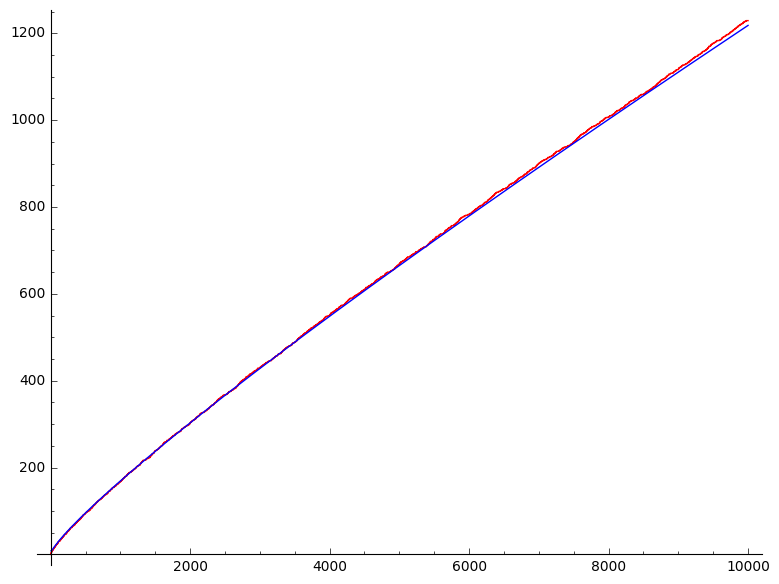
\includegraphics[width=10cm]{prime-pi}
\end{center}

\begin{problem}{integers:code}
Write code in sage to find the greatest common divisor of two integers, using the ideas of problem~\vref{problem:integers:multiple.of.two}.
\end{problem}
%def is_even(b):
%    return b%2==0
%
%def gcd_binary(b,c):
%    if b==0:
%        return c
%    else:
%        if c==0:
%            return b
%        else:
%            if is_even(b):
%                if is_even(c):
%                    return 2*gcd_binary(b//2,c//2)
%                else:
%                    return gcd_binary(b//2,c)
%            else:
%                if is_even(c):
%                    return gcd_binary(b,c//2)
%                else:
%                    B=abs(b)
%                    C=abs(c)
%                    if B>C:
%                        return gcd_binary(B,B-C)
%                    else:
%                        return gcd_binary(C,C-B)

\chapter{Modular arithmetic}
\epigraph[author={Carl Friedrich Gauss}]{Mathematics is the queen of the sciences and number theory is the queen of mathematics.}\SubIndex{Gauss, Carl Friedrich}

\section{Definition}

If we divide integers by \(7\), the possible remainders are
\[
0, 1, 2, 3, 4, 5, 6.
\]
For example, \(65=9 \cdot 7+2\), so the remainder is \(2\).
Two integers are \emph{congruent mod \(7\)} if they have the same remainder modulo \(7\).
So \(65\) and \(2\) are congruent mod \(7\), because \(65=9 \cdot 7 + 2\) and \(2=0 \cdot 7 + 2\).
We denote congruence modulo \(7\) as
\[
\congmod[7]{65}{2}.\Notation{b=c mod m}{\congmod[m]{b}{c}}{\(b\) is congruent to \(c\) modulo \(m\)}
\]
Sometimes we will allow ourselves a sloppy notation, where we write the remainder of \(65\) modulo \(7\) as \(\overline{65}\).\Notation{bb}{\bar{b}}{congruence class of \(b\)}
This is sloppy because the notation doesn't remind us that we are working out remainders modulo \(7\).
If we change \(7\) to some other number, we could get confused by this notation.
We will often compute remainders modulo some chosen number, say \(m\), instead of \(7\).

If we add multiples of \(7\) to an integer, we don't change its remainder modulo \(7\):
\[
\overline{65+7}=\overline{65}.
\]
Similarly, 
\[
\overline{65-7}=\overline{65}.
\]


If we add, or multiply, some numbers, what happens to their remainders?
\begin{theorem}
Take a positive integer \(m\) and integers \(a, A, b, B\).
If \(\congmod[m]{a}{A}\) and \(\congmod[m]{b}{B}\) then
\begin{align*}
a+b &\equiv A+B \pmod{m}, \\
a-b &\equiv A-B \pmod{m}, \\
\text{and } ab &\equiv AB \pmod{m}.
\end{align*}
The bar notation is more elegant.
If we agree that \(\bar{a}\) means remainder of \(a\) modulo the fixed choice of integer \(m\), we can write this as: if
\[
\bar{a}=\bar{A} \text{ and } \bar{b}=\bar{B}
\]
then
\begin{align*}
\overline{a+b}&=\overline{A+B}, \\
\overline{a-b}&=\overline{A-B}, \text{ and } \\
\overline{ab}&=\overline{AB}.
\end{align*}
\end{theorem}
\begin{example}
Note that \(\congmod[7]{9}{2}\) and \(\congmod[7]{4}{11}\), so our theorem tells us that \(\congmod[7]{9 \cdot 4}{2 \cdot 11}\).
Let's check this. 
The left hand side:
\begin{align*}
9 \cdot 4
&=
36,
\\
&=
5(7)+1,
\end{align*}
so that \(\congmod[7]{9 \cdot 4}{1}\).
The right hand side:
\begin{align*}
2 \cdot 11
&=
22,
\\
&=
3(7)+1,
\end{align*}
so that \(\congmod[7]{2 \cdot 11}{1}\).
\end{example}
So it works in this example.
Let's prove that it always works.
\begin{proof}
Since \(a-A\) is a multiple of \(m\), as is \(b-B\), note that
\[
(a+b)-(A+B)=(a-A)+(b-B)
\]
is also a multiple of \(m\), so addition works.
In the same way
\[
ab-AB=(a-A)b+A(b-B)
\]
is a multiple of \(m\).
\end{proof}

\begin{problem}{modular.arithmetic:perfect.square}
Prove by induction that every ``perfect square'', i.e. integer of the form \(n^2\), has remainder \(0, 1\) or \(4\) modulo \(8\).
\end{problem}

\begin{problem}{modular.arithmetic:nine}
Take an integer like \(243098\) and write out the sum of its digits \(2+4+3+0+9+8\).
Explain why every integer is congruent to the sum of its digits, modulo \(9\).
\end{problem}
\begin{answer}{modular.arithmetic:nine}
A 1-digit positive integer has the form \(b=b_0\) with \(0 \le b_0 \le 9\) its first digit.
A 2-digit positive integer has the form \(b=b_0+10 \, b_1\) with \(0 \le b_0,b_1 \le 9\).
In general, an \(n\)-digit positive integer has the form 
\[
b=b_0+10 \, b_1 + 10^2 \, b_2 + \dots + 10^{n-1} b_{n-1}.
\]
Modulo \(9\), \(\congmod[9]{10}{1}\), so modulo 9
\begin{align*}
\congmod[9]{b&}{b_0+10 \, b_1 + 10^2 \, b_2 + \dots + 10^{n-1} b_{n-1}},
\\
\congmod[9]{&}{b_0+b_1+b_2 + \dots + b_{n-1}}.
\end{align*}
\end{answer}

\begin{problem}{modular.arithmetic:gcd}
Take integers \(a,b,m\) with \(m \ne 0\).
Let \(d\defeq\gcd{a,b,m}\).
Prove that \(\congmod[m]{a}{b}\) just when \(\congmod[m/d]{a/d}{b/d}\).
\end{problem}

\section{Arithmetic of remainders}

We now \emph{define} an addition law on the numbers \(0,1,2,3,4,5,6\) by declaring that when we add these numbers, we then take remainder modulo \(7\).
This is \emph{not} usual addition.
To make this clear, we write the remainders with bars over them, always.
For example, we are saying that in this addition law \(\bar{3}+\bar{5}\) means \(\overline{3+5}=\overline{8}=\bar{1}\), since we are working modulo \(7\).
We adopt the same rule for subtraction, and for multiplication.
For example, modulo \(13\),
\begin{align*}
\pr{\bar{7}+\bar{9}}\pr{\overline{11}+\bar{6}}
&=
\overline{16} \cdot \overline{17},
\\
&=
\overline{13+3} \cdot \overline{13+4},
\\
&=
\overline{3} \cdot \overline{4},
\\
&=
\overline{12}.
\end{align*}
If we are daring, we might just drop all of the bars, and state clearly that we are calculating modulo some integer.
In our daring notation, modulo 17,
\begin{align*}
16 \cdot 29 - 7 \cdot 5 
&=
16 \cdot 12 - 7 \cdot 5,
\\
&=
192 - 35,
\\
&=
\pr{11\cdot 17 + 5} - \pr{2 \cdot 17 + 1},
\\
&=
5 - 1,
\\
&=
4.
\end{align*}


\begin{problem}{modular.arithmetic:examples}
Expand and simplify \(\bar{5}\cdot\bar{2} \cdot \pr{\bar{6}-\bar{9}}\) modulo \(7\).
\end{problem}

The addition and multiplication tables for remainder modulo \(5\):
\[
\begin{array}{@{}r|rrrrr@{}}
+ & 0 & 1 & 2 & 3 & 4 \\ \hline
0 & 1 & 2 & 3 & 4 & 0 \\
1 & 2 & 3 & 4 & 0 & 1 \\
2 & 3 & 4 & 0 & 1 & 2 \\
3 & 4 & 0 & 1 & 2 & 3 \\
4 & 0 & 1 & 2 & 3 & 4
\end{array}
\qquad
\begin{array}{@{}r|rrrrr@{}}
\cdot & 0 & 1 & 2 & 3 & 4 \\ \hline
    0 & 0 & 0 & 0 & 0 & 0 \\
    1 & 0 & 1 & 2 & 3 & 4 \\
    2 & 0 & 2 & 4 & 1 & 3 \\
    3 & 0 & 3 & 1 & 4 & 2 \\
    4 & 0 & 4 & 3 & 2 & 1
\end{array}
\]

\begin{problem}{modular.arithmetic:laws}
Describe laws of modular arithmetic, imitating the laws of integer arithmetic.
If we work modulo \(4\), explain why the zero divisors law fails.
Why are there no sign laws?
\end{problem}

\begin{problem}{modular.arithmetic:remainder}
Compute the remainder when dividing \(19\) into \(37^{200}\).
\end{problem}

\begin{problem}{modular.arithmetic:remainder.2}
Compute the last two digits of \(9^{2000}\).
\end{problem}

\begin{problem}{modular.arithmetic:quad.eqn}
Prove that the equation \(a^2 + b^2 = 3c^2\) has no solutions in nonzero integers \(a\), \(b\) and \(c\).
Hint: start by proving that modulo \(4\), \(a^2=0\) or \(1\).
Then consider the equation modulo 4; show that \(a\), \(b\) and \(c\) are divisible by 2. Then each of \(a^2\), \(b^2\) and \(c^2\) has a factor of 4. 
Divide through by 4 to show that there would be a smaller set of solutions to the original equation.
Apply induction.
\end{problem}

\begin{example}
To carry a remainder to a huge power, say \(2^{2005}\) modulo \(13\), we can build up the power out of smaller ones.
For example, \(2^2=4\) modulo \(13\), and therefore modulo \(13\),
\begin{align*}
2^4
&=
\pr{2^2}^2,
\\
&=4^2,
\\
&=16,
\\
&=3.
\end{align*}
Keeping track of these partial results as we go, modulo \(13\),
\begin{align*}
2^8
&=
\pr{2^4}^2,
\\
&=
3^2,
\\
&=9.
\end{align*}
We get higher and higher powers of \(2\): modulo \(13\),
\[
\begin{array}{@{}rrr@{}}
\toprule 
k & 2^k & 2^{2^k} \operatorname{mod} 13 \\
\midrule
0 & 1 & 2 \\
1 & 2 & 4 \\
2 & 4 & 3 \\
3 & 8 & 9 \\
4 & 16 & 9^2=81=3\\
5 & 32 & 3^2=9 \\
6 & 64 & 9^2=3 \\
7 & 128 & 3^2=9\\
8 & 256 & 9^2=3 \\
9 & 512 & 3^2=9 \\
10 & 1024 & 9^2=3 \\
11 & 2048 & 
\\ \bottomrule
\end{array}
\]
The last row gets into \(2^{2048}\), too large to be relevant to our problem.
We now want to write out exponent \(2005\) as a sum of powers of \(2\), by first dividing in \(1024\):
\begin{align*}
2005
&=
1024
+
981
\\
\intertext{and then dividing in the next power of 2 we can fit into the remainder,}
&= 1024 + 512 + 469,
\\
&= 1024 + 512 + 256 + 128 + 64 + 16 + 4 + 1.
\end{align*}
Then we can compute out modulo \(13\):
\begin{align*}
2^{2005}
&=
2^{1024 + 512 + 256 + 128 + 64 + 16 + 4 + 1},
\\
&=
2^{1024} 2^{512} 2^{256} 2^{128} 2^{64} 2^{16} 2^4 2^1,
\\
&=
3 \cdot 9 \cdot 3 \cdot 9 \cdot 3 \cdot 3 \cdot 3 \cdot 2,
\\
&=
\pr{3 \cdot 9}^3 \cdot 2,
\\
&=
27^2 \cdot 2,
\\
&=
1^2 \cdot 2,
\\
&=
2.
\end{align*}
\end{example}

\begin{problem}{modular:big.power}
Compute \(2^{100}\) modulo \(125\).
\end{problem}


\section{Reciprocals}

Every nonzero rational number \(b/c\) has a reciprocal: \(c/b\).
Since we now have modular arithmetic defined, we want to know which remainders have ``reciprocals''.
Working modulo some positive integer, say that a remainder \(x\) has a reciprocal \(y=x^{-1}\) if \(xy=1\).
(It seems just a little too weird to write it as \(y=1/x\), but you can if you like.)
Reciprocals are also called \emph{multiplicative inverses}.\define{multiplicative inverse}
\begin{example}
Modulo \(7\)
\begin{align*}
\bar{1} \cdot \bar{1} &= \bar{1}, \\
\bar{2} \cdot \bar{4} &= \bar{1}, \\
\bar{3} \cdot \bar{5} &= \bar{1}, \\
\bar{4} \cdot \bar{2} &= \bar{1}, \\
\bar{5} \cdot \bar{3} &= \bar{1}, \\
\bar{6} \cdot \bar{6} &= \bar{1}.
\end{align*}
So in this weird type of arithmetic, we can allow ourselves the freedom to write these equations as identifying a reciprocal.
\begin{align*}
\bar{1}^{-1} &= \bar{1}, \\
\bar{2}^{-1} &= \bar{4}, \\
\bar{3}^{-1} &= \bar{5}, \\
\bar{4}^{-1} &= \bar{2}, \\
\bar{5}^{-1} &= \bar{3}, \\
\bar{6}^{-1} &= \bar{6}.
\end{align*}
\end{example}
A remainder that has a reciprocal is a \emph{unit}.\define{unit}

\begin{problem}{modular.arithmetic:no.reciprocal}
\emph{Danger:} If we work modulo \(4\), then prove that \(\bar{2}\) has \emph{no} reciprocal.
Hint: \(\bar{2}^2=0\).
\end{problem}

\begin{problem}{modular.arithmetic:reciprocal}
Prove that, modulo any integer \(m\), \((m-1)^{-1}=m-1\), and that modulo \(m^2\), \((m-1)^{-1}=m^2-m-1\).
\end{problem}

\begin{theorem}
Take a positive integer \(m\) and a remainder \(\bar{r}\) modulo \(m\).
Take the B\'ezout coefficients of \(r\) and \(m\): \(sr+tm=d\), so that \(d\) is the greatest common divisor of \(r\) and \(m\).

If \(d=1\) then \(\bar{r}^{-1}=\bar{s}\) modulo \(m\).
If \(d \ne 1\) then \(\bar{r}^{-1}\) does not exist.
In particular, in the remainders modulo \(m\), a remainder \(\bar{r}\) is a unit just when \(r,m\) are coprime integers.
\end{theorem}
\begin{proof}
If \(r,m\) are coprime integers, so their greatest common divisor is \(1\), then write B\'ezout coefficients \(sr+tm=1\), and quotient by \(m\):
\[
\bar{s}\bar{r}=\bar{1}.
\]

On the other hand, if 
\[
\bar{s}\bar{r}=\bar{1},
\]
then \(sr\) is congruent to \(1\) modulo \(m\), i.e. there is some quotient \(q\) so that \(sr=qm+1\), so \(sr-qm=1\), giving B\'ezout coefficients \(s=s,t=-q\), so the greatest common divisor of \(r,m\) is \(1\).
\end{proof}

\begin{example}
Working modulo \(163\), let's compute \(14^{-1}\).
First we carry out the long division
\[
\longdiv{163}{14}
\]
Now let's start looking for B\'ezout coefficients, by writing out matrix:
\[
\begin{pmatrix}
1 & 0 & 14 \\
0 & 1 & 163
\end{pmatrix}
\]
and then add \(-11\cdot\text{row 1}\) to row 2:
\[
\begin{pmatrix}
1 & 0 & 14 \\
-11 & 1 & 9
\end{pmatrix}.
\]
Add \(-\text{row 2}\) to row 1:
\[
\begin{pmatrix}
12 & -1 & 5 \\
-11 & 1 & 9
\end{pmatrix}.
\]
Add \(-\text{row 1}\) to row 2:
\[
\begin{pmatrix}
12 & -1 & 5 \\
-23 & 2 & 4
\end{pmatrix}.
\]
Add \(-\text{row 2}\) to row 1:
\[
\begin{pmatrix}
35 & -3 & 1 \\
-23 & 2 & 4
\end{pmatrix}.
\]
Add \(-4 \cdot \text{row 1}\) to row 2:
\[
\begin{pmatrix}
35 & -3 & 1 \\
-163 & 14 & 0
\end{pmatrix}.
\]
Summing it all up: \(35 \cdot 14 + (-3) \cdot 163 = 1\).
Quotient out by \(163\): modulo \(163\), \(35 \cdot 14 = 1\), so modulo \(163\), \(14^{-1}=35\).
\end{example}

\begin{problem}{modular.arithmetic:reciprocals}
Use this method to find reciprocals:
\begin{enumerate}
\item 
\(13^{-1}\) modulo \(59\)
\item
\(10^{-1}\) modulo \(11\)
\item
\(2^{-1}\) modulo \(193\).
\item
\(6003722857^{-1}\) modulo \(77695236973\).
\end{enumerate}
\end{problem}
\begin{answer}{modular.arithmetic:reciprocals}
\begin{enumerate}
\item 
\sagestr{bezpretty(13,59)}
Answer:\(13^{-1} = \sage{inverse_mod(13,59)}\) modulo \(59\)
\item
\sagestr{bezpretty(10,11)}
Answer:\(10^{-1} = \sage{inverse_mod(10,11)}\) modulo \(11\)
\item
\sagestr{bezpretty(2,193)}
Answer:\(2^{-1} = \sage{inverse_mod(2,193)}\) modulo \(193\)
\item
\sagestr{bezpretty(6003722857,77695236973)}
Answer:\(6003722857^{-1} = \sage{inverse_mod(6003722857,77695236973)}\) modulo \(77695236973\)
\end{enumerate}
\end{answer}

\begin{problem}{modular.arithmetic:prime.field}
Suppose that \(b, c\) are remainders modulo a prime.
Prove that \(bc=0\) just when either \(b=0\) or \(c=0\).
\end{problem}

\begin{problem}{modular.arithmetic:Fermats.Little.Theorem}
Suppose that \(p\) is a prime number and \(n\) is an integer with \(n < p\).
Explain why, modulo \(p\), the numbers \(0, n, 2n, 3n, \dots, (p-1)n\) consist in precisely the remainders \(0,1,2,\dots,p-1\), in some order.
(Hint: use the reciprocal of \(n\).)
Next, since every nonzero remainder has a reciprocal remainder, explain why the product of the nonzero remainders is \(1\).
Use this to explain why 
\[
\congmod[p]{n^{p-1}}{1}.
\]
Finally, explain why, for any integer \(k\),
\[
\congmod[p]{k^p}{k}.
\]
\end{problem}

\section{The Chinese remainder theorem}

\epigraph[author={Brahmagupta (580CE--670CE)}, source={Brahma-Sphuta-Siddhanta (Brahma's Correct System)}]{An old woman goes to market and a horse steps on her basket and  crushes the eggs. The rider offers to pay for the damages and asks  her how many eggs she had brought. She does not remember the 
exact number, but when she had taken them out two at a time,  there was one egg left. The same happened when she picked them out three, four, five, and six at a time, but when she took them seven at a time, there were none left. What is the smallest number of eggs she could have had?}\SubIndex{Brahmagupta}\SubIndex{Brahma-Sphuta-Siddhanta}\SubIndex{Brahma's correct system}

Take a look at some numbers and their remainders modulo \(3\) and \(5\):
\[
\begin{array}{@{}rrr@{}}
\toprule
n & n \operatorname{mod} 3 & n \operatorname{mod} 5 \\ \midrule
0 & 0 & 0 \\
1 & 1 & 1 \\
2 & 2 & 2 \\
3 & 0 & 3 \\
4 & 1 & 4 \\
5 & 2 & 0 \\
6 & 0 & 1 \\
7 & 1 & 2 \\
8 & 2 & 3 \\
9 & 0 & 4 \\
10 & 1 & 0 \\
11 & 2 & 1 \\
12 & 0 & 2 \\
13 & 1 & 3 \\
14 & 2 & 4 \\
15 & 0 & 0 \\
\bottomrule
\end{array}
\]
Remainders modulo \(3\) repeat every \(3\), and remainders modulo \(5\) repeat every \(5\), but the pair of remainders modulo \(3\) and \(5\) together repeat every \(15\).

\begin{example}
How can you find an integer \(x\) so that 
\begin{align*}
&\congmod[3]{x}{1}, \\
&\congmod[4]{x}{2}, \\
&\congmod[7]{x}{1}?
\end{align*}
\end{example}

\begin{example}
A recipe: how to find an unknown integer \(x\) given only the knowledge of its remainders modulo various integers.
Suppose we know \(x\) has remainder \(r_1\) modulo \(m_1\), \(r_2\) modulo \(m_2\), and so on.
Let 
\[
m\defeq m_1 m_2 \dots m_n.
\]
For each \(i\), let
\[
u_i\defeq \frac{m}{m_i}=m_1 m_2 \dots m_{i-1} m_{i+1} m_{i+2} \dots m_n.
\]
Each \(u_i\) has some reciprocal modulo \(m_i\), given as the remainder of some integer \(v_i\).
Let 
\[
x\defeq r_1 u_1 v_1 + r_2 u_2 v_2 + \dots + r_n u_n v_n.
\]
We can simplify this a little: add or subtract multiples of \(m\) until \(x\) is in the range \(0 \le x \le m-1\).
\end{example}

\begin{theorem}
Take some positive integers \(m_1, m_2, \dots, m_n\), so that any two of them are coprime.
Suppose that we want to find an unknown integer \(x\) given only the knowledge of its remainders modulo \(m_1, m_2, \dots, m_n\); so we know its remainder modulo \(m_1\) is \(r_1\), modulo \(m_2\) is \(r_2\), and so on.
There is such an integer \(x\), given by the recipe above, and \(x\) is unique modulo 
\[
m_1 m_2 \dots m_n.
\]
\end{theorem}
\begin{proof}
All of \(m_1, m_2, \dots, m_n\) divide \(u_i\), except \(m_i\).
So if \(j \ne i\) then modulo \(m_j\), \(u_i=0\).
All of the other \(m_j\) are coprime to \(m_i\), so their product is coprime to \(m_i\), so has a reciprocal modulo \(m_i\).
Thus modulo \(m_i\), \(u_i\ne 0\). 
Then modulo \(m_i\), \(x=r_i\), and so on.
So the recipe gives the required integer \(x\).
If there are two, then their difference vanishes modulo all of the \(m_i\), so is a multiple of every one of the \(m_i\), which are coprime, so is a multiple of their product \(m\).
\end{proof}

\begin{example}
Let's find an integer \(x\) so that 
\begin{align*}
&\congmod[3]{x}{1}, \\
&\congmod[4]{x}{2}, \\
&\congmod[7]{x}{1}.
\end{align*}
So in this problem we have to work modulo \(\pr{m_1,m_2,m_3}=\pr{3,4,7}\), and get remainders \(\pr{r_1,r_2,r_3}=\pr{1,2,1}\).
First, no matter what the remainders, we have to work out the reciprocal mod each \(m_i\) of the product of all of the other \(m_j\).
So let's reduce these products down to their remainders:
\begin{align*}
4 \cdot 7 &= 28 = 9\cdot 3 + 1 \equiv 1 \pmod{3}, \\
3 \cdot 7 &= 21 = 5\cdot 4 + 1 \equiv 1 \pmod{4}, \\
3 \cdot 4 &= 12 = 1\cdot 7 + 5 \equiv 5 \pmod{7}.
\end{align*}
We need the reciprocals of these, which, to save ink, we just write down for you without writing out the calculations:
\begin{align*}
1^{-1} &\equiv 1 \pmod{3}, \\
1^{-1} &\equiv 1 \pmod{4}, \\
5^{-1} &\equiv 3 \pmod{7}.
\end{align*}
(You can easily check those.)
Finally, we add up remainder times product times reciprocal:
\begin{align*}
x
&=
r_1 \cdot 4 \cdot 7 \cdot 1 
+
r_2 \cdot 3 \cdot 7 \cdot 1 
+
r_3 \cdot 3 \cdot 4 \cdot 3,
\\
&=
1 \cdot 4 \cdot 7 \cdot 1 
+
2 \cdot 3 \cdot 7 \cdot 1 
+
1 \cdot 3 \cdot 4 \cdot 3,
\\
&=
106.
\end{align*}
We can now check to be sure:
\begin{align*}
&\congmod[3]{106}{1}, \\
&\congmod[4]{106}{2}, \\
&\congmod[7]{106}{1}.
\end{align*}
The Chinese remainder theorem tells us also that \(106\) is the unique solution modulo \(3 \cdot 4 \cdot 7=84\).
But then \(106-84=22\) is also a solution, the smallest positive solution.
\end{example}

\begin{problem}{modular.arithmetic:eggs}
Solve the problem about eggs. Hint: ignore the information about eggs taken out six at a time.
\end{problem}

\begin{problem}{modular.arithmetic:army}
Use the Chinese remainder theorem to determine the smallest number of soldiers possible in Han Xin's army if the following facts are true.
When they parade in rows of 3 soldiers, two soldiers will be left. When they parade in rows of 5, 3 will be left, and in rows of 7, 2 will be left.
\end{problem}

\begin{problem}{modular.arithmetic:army.2}
Use the Chinese remainder theorem to determine the smallest number of soldiers possible in Han Xin's army if the following facts are true.
When they parade in rows of 3 soldiers, one soldier will be left. When they parade in rows of 7, 2 will be left, and in rows of 19, three will be left.
\end{problem}
\begin{answer}{modular.arithmetic:army.2}
We want to find remainders \((1,2,3)\) modulo \((3,7,19)\).
We let 
\begin{align*}
u_1 &= 7 \cdot 19 = 133, \\
u_2 &= 3 \cdot 19 = 57, \\
u_3 &= 3 \cdot 7 = 21.
\end{align*}
Modulo \(3,7,19\) these are
\begin{align*}
u_1 &= 1 \mod{3}, \\
u_2 &= 1 \mod{7}, \\
u_3 &= 2 \mod{19}.
\end{align*}
The multiplicative inverses of these, modulo \(3,7,19\), are obvious by reducing and inspection:
\begin{align*}
v_1 &= 1, \\
v_2 &= 1, \\
v_3 &= 10.
\end{align*}
By the Chinese remainder theorem, the answer, up to multiples of \(3 \cdot 7 \cdot 19=399\), is
\begin{align*}
r_1 u_1 v_1 + r_2 u_2 v_2 + r_3 u_3 v_3 
&=
1 \cdot 133 \cdot 1 
+
2 \cdot 57 \cdot 1
+
3 \cdot 21 \cdot 10,
\\
&=
133+114+630,
\\
&=877,
\\
&=79+2 \cdot 399.
\end{align*}
So there are at least 79 soldiers in Han Xin's army.
\end{answer}


Given some integers \(m_1, m_2, \dots, m_n\), we consider sequences \(\pr{b_1, b_2, \dots, b_n}\) consisting of remainders: \(b_1\) a remainder modulo \(m_1\), and so on.
Add sequences of remainders in the obvious way:
\[
\pr{b_1,b_2,\dots,b_n}
+
\pr{c_1,c_2, \dots, c_n}
=
\pr{b_1+c_1,b_2+c_2, \dots, b_n+c_n}.
\]
Similarly, we can subtract and multiply sequences of remainders:
\[
\pr{b_1,b_2,\dots,b_n}
\pr{c_1,c_2, \dots, c_n}
=
\pr{b_1c_1,b_2c_2, \dots, b_nc_n},
\]
by multiplying remainders as usual, modulo the various \(m_1, m_2, \dots, m_n\).
\begin{example} 
Modulo \(\pr{3,5}\), we multiply 
\begin{align*}
(2,4)(3,2)
&=(2 \cdot 3, 4 \cdot 2),
\\
&=(6, 8),
\\
&=(0,3).
\end{align*}
\end{example}

Let \(m \defeq m_1 m_2 \dots m_n\).
To each remainder modulo \(m\), say \(b\), associate its remainder \(b_1\) modulo \(m_1\), \(b_2\) modulo \(m_2\), and so on.
Associate the sequence \(\vec{b}\defeq\pr{b_1,b_2,\dots,b_n}\) of all of those remainders.
In this way we make a map taking each remainder \(b\) modulo \(m\) to its sequence \(\vec{b}\) of remainders modulo all of the various \(m_i\).
Moreover, \(\overrightarrow{b+c}=\vec{b}+\vec{c}\) and \(\overrightarrow{b-c}=\vec{b}-\vec{c}\) and \(\overrightarrow{bc}=\vec{b}\vec{c}\), since each of these works when we take remainder modulo anything.

\begin{example}
Take \(m_1,m_2,m_3\) to be \(3,4,7\).
Then \(m=3 \cdot 4 \cdot 7 = 84\).
If \(b=8\) modulo \(84\), then 
\begin{align*}
b_1 &= 8 \mod 3, \\
    &= 2, \\
b_2 &= 8 \mod 4, \\
    &= 0, \\
b_3 &= 8 \mod 7, \\
    &= 1, \\
\vec{b} &= \pr{b_1,b_2,b_3} = \pr{2,0,1}.  
\end{align*}
\end{example}


\begin{corollary}\label{corollary:CRT}
Take some positive integers \(m_1, m_2, \dots, m_n\), so that any two of them are coprime.
The map taking \(b\) to \(\vec{b}\), from remainders modulo \(m\) to sequences of remainders modulo \(m_1, m_2, \dots, m_n\), is one-to-one and onto, identifies sums with sums, products with products, differences with differences, units with sequences of units.
\end{corollary}


\section{Euler's totient function}

\emph{Euler's totient function}\define{Euler's totient function}\define{totient function} \(\phi\)\Notation{phi(m)}{\phi(m)}{Euler's totient function} assigns to each positive integer \(m=2,3, \dots\) the number of all remainders modulo \(m\) which are units (in other words, coprime to \(m\)) [in other words, which have reciprocals].
It is convenient to \emph{define} \(\phi(1)\defeq 1\) (even though there \emph{isn't} actually 1 unit remainder modulo 1).

\begin{problem}{modular.arithmetic:totient.values}
Explain by examining the remainders that the first few values of \(\phi\) are
\[
\begin{array}{@{}rl@{}}
\toprule
m & \phi(m) \\
\midrule
1 & 1 \\
2 & 1 \\
3 & 2 \\
4 & 2 \\
5 & 4 \\
6 & 2 \\
7 & 6 \\
\bottomrule
\end{array}
\]
\end{problem}

\begin{problem}{modular.arithmetic:prime.phi}
Prove that a positive integer \(m \ge 2\) is prime just when \(\phi(m)=m-1\).
\end{problem}

\begin{theorem}\label{theorem:totient}
Suppose that \(m\ge 2\) is an integer with prime factorizaton
\[
m = p_1^{a_1} p_2^{a_2} \dots p_n^{a_n},
\]
so that \(p_1, p_2, \dots, p_n\) are prime numbers and \(a_1, a_2, \dots, a_n\) are positive integers.
Then
\[
\phi(m)=
\pr{p_1^{a_1}-p_1^{a_1-1}}
\pr{p_2^{a_2}-p_2^{a_2-1}}
\dots
\pr{p_n^{a_n}-p_n^{a_n-1}}.
\]
\end{theorem}
\begin{proof}
If \(m\) is prime, this follows from problem~\vref{problem:modular.arithmetic:prime.phi}.

Suppose that \(m\) has just one prime factor, or in other words that \(m=p^a\) for some prime number \(p\) and integer \(a\).
It is tricky to count the remainders coprime to \(m\), but easier to count those not coprime, i.e. those which have a factor of \(p\).
Clearly these are the multiples of \(p\) between \(0\) and \(p^a-p\), so the numbers \(pj\) for \(0 \le j \le p^{a-1}-1\).
So there are \(p^{a-1}\) such remainders.
We take these out and we are left with \(p^a-p^{a-1}\) remainders left, i.e. coprime.

If \(b,c\) are coprime integers \(\ge 2\), then corollary~\vref{corollary:CRT} maps units modulo \(bc\) to pairs of a unit modulo \(b\) and a unit modulo \(c\), and is one-to-one and onto.
Therefore counting units: \(\phi(bc)=\phi(b)\phi(c)\).
\end{proof}

\begin{theorem}[Euler]\label{theorem:Euler}
For any positive integer \(m\) and any integer \(b\) coprime to \(m\), 
\[
\congmod[m]{b^{\phi(m)}}{1}.
\]
\end{theorem}
\begin{proof}
Working with remainders modulo \(m\), we have to prove that for any unit remainder \(b\), \(b^{\phi(m)}=1\) modulo \(m\).

Let \(U\) be the set of all units modulo \(m\), so \(U\) is a subset of the remainders \(0,1,2,\dots,m-1\).
The product of units is a unit, since it has a reciprocal (the product of the reciprocals).
Therefore the map
\[
u \in U \mapsto bu \in U
\]
is defined.
It has an inverse:
\[
u \in U \mapsto b^{-1}u \in U,
\]
where \(b^{-1}\) is the reciprocal of \(b\).
Writing out the elements of \(U\), say as
\[
u_1, u_2, \dots, u_q
\]
note that \(q=\phi(m)\).
Then multiplying by \(b\) scrambles these units into a different order:
\[
bu_1, bu_2, \dots, bu_q.
\]
But multiplying by \(b\) just scrambles the order of the roots, so if we multiply them all, and then scramble them back into order:
\[
\pr{bu_1}\pr{bu_2} \dots \pr{bu_q}= u_1 u_2 \dots u_q.
\]
Divide every unit \(u_1, u_2, \dots, u_q\) out of boths sides to find \(b^q=1\).
\end{proof}

\begin{problem}{modular.arithmetic:find.reciprocal}
Take an integer \(m \ge 2\).
Suppose that \(b\) is a unit in the remainders modulo \(m\).
Prove that the reciprocal of \(b\) is \(b^{\phi(m)-1}\).
\end{problem}

Euler's theorem is important because we can use it to calculate quickly modulo prime numbers (and sometimes even modulo numbers which are not prime).
\begin{example}
Modulo \(19\), let's find \(123456789^{987654321}\).
First, the base of this expression is \(123456789=6497725 \cdot 19 + 14\)
So modulo \(19\):
\[
123456789^{987654321}=14^{987654321}.
\]
That helps with the base, but the exponent is still large.
According to Euler's theorem, since \(19\) is prime, modulo \(19\):
\[
b^{19-1} = 1
\]
for any remainder \(b\).
In particular, modulo \(19\),
\[
14^{18}=1.
\]
So every time we get rid of \(18\) copies of \(14\) multiplied together, we don't change our result. 
Divide \(18\) into the exponent:
\[
987654321 = 54869684 \cdot 18 + 9.
\]
So then modulo \(19\):
\[
14^{987654321} = 14^9.
\]
We leave the reader to check that \(14^9=18\) modulo \(19\), so that finally, modulo \(19\),
\[
123456789^{987654321}=18.
\]
\end{example}

\begin{problem}{modular:use.totient}
By hand, using Euler's totient function, compute \(127^{162}\) modulo \(120\).
\end{problem}
\begin{answer}{modular:use.totient}
Factor \(120 =2^3 \, 3^1 \, 5^1\).
So Euler's totient is \(\phi(120)=(2^3-2^2)(3^1-3^0)(5^1-5^0)=32\).
Since \(127\) is prime, it is coprime to \(120\).
The theorem of Euler's totient function says that \(127^{\phi(120)}=1\) modulo \(120\). 
So \(127^{32}=1\) modulo \(120\).
In other words, every time you multiply together \(32\) copies of \(127\), modulo \(120\), it is as if you multiplied together no copies.
Check that \(162 = 5\cdot 32+2\).
So modulo 120, \(127^{162}=127^{5 \cdot 32+2}=127^2\). 
This is not quite the answer. 
But we know that \(127=7\) modulo \(120\). 
So modulo 120, \(127^{162}=7^2=49\).
\end{answer}

\begin{lemma}\label{lemma:multiply.by.a}
For any prime number \(p\) and integers \(b\) and \(k\), \(b^{1+k(p-1)}=b\) modulo \(p\).
\end{lemma}
\begin{proof}
If \(b\) \emph{is} a multiple of \(p\) then \(b=0\) modulo \(p\) so both sides are zero. 
If \(b\) is not a multiple of \(p\) then \(b^{p-1}=1\) modulo \(p\), by Euler's theorem.
Take both sides to the power \(k\) and multiply by \(b\) to get the result.
\end{proof}

\begin{theorem}\label{theorem:generalized.Euler}
Suppose that \(m=p_1 p_2 \dots p_n\) is a product of distinct prime numbers.
Then for any integers \(b\) and \(k\) with \(k \ge 0\),
\[
\congmod[m]{b^{1+k\phi(m)}}{b}.
\]
\end{theorem}
\begin{proof}
By lemma~\vref{lemma:multiply.by.a}, the result is true if \(m\) is prime.
So if we take two prime numbers \(p\) and \(q\), then\(b^{1+k(p-1)(q-1)}=b\) modulo \(p\), but also modulo \(q\), and therefore modulo \(pq\).
The same trick works if we start throwing in more distinct prime factors into \(m\).
\end{proof}

\begin{problem}{modular.arithmetic:example.not.Euler}
Give an example of integers \(b\) and \(m\) with \(m \ge 2\) for which \(b^{1+\phi(m)} \ne b\) modulo \(m\).
\end{problem}


\section{Sage}

In Sage, the quotient of \(71\) modulo \(13\) is \verb!mod(71,13)!.
The tricky bit: it returns a ``remainder modulo 13'', so if we write
\begin{sageblock}
a=mod(71,13)
\end{sageblock}
this will define \(a\) to be a ``remainder modulo 13''. 
The value of \(a\) is then \(\sage{a}\), but the value of \(a^2\) is \(\sage{a^2}\), because the result is again calculated modulo 13.

Euler's totient function is
\begin{sageblock}
euler_phi(777)
\end{sageblock}
which yields \(\phi(777)=\sage{euler_phi(777)}\).
To find \(14^{-1}\) modulo \(19\),
\begin{sageblock}
inverse_mod(14,19)
\end{sageblock}
yields
\(14^{-1}=\sage{inverse_mod(14,19)}\) modulo \(19\).

We can write our own version of Euler's totient function, just to see how it might look:
\begin{sageblock}
def phi(n):
    return prod(p^a-p^(a-1) for (p,a) in factor(n))
\end{sageblock}
where \verb!prod! means product, so that \verb!phi(666)! yields \(\phi(666)=\sage{phi(666)}\).
The code here uses the function \verb!factor()!, which takes an integer \(n\) and returns a list \verb!p=factor(n)! of its prime factors.
In our case, the prime factorisation of \(666\) is \(666=2 \cdot 3^2 \cdot 37\).
The expression \verb!p=factor(n)! when \(n=666\) yields a list \verb!p=[(2,1), (3,2), (37,1)]!, a list of the prime factors together with their powers.
To find these values, \verb!p[0]! yields \verb!(2,1)!, \verb!p[1]! yields \verb!(3,2)!, and \verb!p[2]! yields \verb!(37,1)!.
The expression \verb!len(p)! gives the length of the list \verb!p!, which is the number of entries in that list, in this case \(3\).
For each entry, we set \(b=p_i\) and \(e=a_i\) and then multiply the result \(r\) by \(b^e-b^{e-1}\).

To use the Chinese remainder theorem, suppose we want to find a number \(x\) so that \(x\) has remainders \(1\) mod \(3\) and \(2\) mod \(7\),
\begin{sageblock}
crt([1,2],[3,7])
\end{sageblock}
gives you \(x=\sage{crt([1,2],[3,7])}\); you first list the two remainders \verb!1,2! and then list the moduli \verb!3,7!.

Another way to work with modular arithmetic in sage: we can create an object which represents the remainder of \(9\) modulo \(17\):
\begin{sageblock}
a=mod(9,17)
a^(-1)
\end{sageblock}
yielding \(\sage{a^(-1)}\).
As long as all of our remainders are modulo the same number \(17\), we can do arithmetic directly on them:
\begin{sageblock}
b=mod(7,17)
a*b
\end{sageblock}
yields \(\sage{a*b}\).



\chapter{Secret messages}\label{chapter:RSA}
\begin{epigraphs}
\qitem[author={Sylvia Plath}, source={The Unabridged Journals of Sylvia Plath}]{And when at last you find someone to whom you feel you can pour out your soul, you stop in shock at the words you utter— they are so rusty, so ugly, so meaningless and feeble from being kept in the small cramped dark inside you so long.}\SubIndex{Plath, Sylvia}\SubIndex{The Unabridged Journals of Sylvia Plath}
\qitem[author={André Malraux}]{Man is not what he thinks he is, he is what he hides.}\SubIndex{Malraux, André} 
\end{epigraphs}
\begin{center}
\begin{minipage}{6cm}
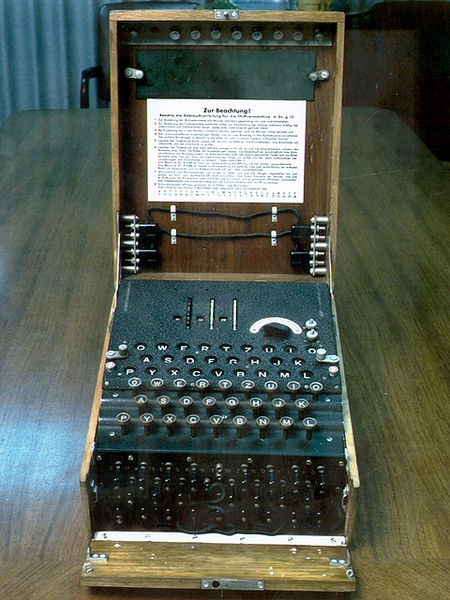
\includegraphics[width=6cm]{Enigma.jpg}
\\
\emph{Enigma},\SubIndex{enigma} Nazi secret code machine
\end{minipage}
\end{center}
\section{RSA: the Cocks, Rivest, Shamir and Adleman algorithm}\SubIndex{RSA algorithm}
\begin{example}
Alice\SubIndex{Alice} wants to send a message to Bob,\SubIndex{Bob} but she doesn't want Eve\SubIndex{Eve} to read it.
She first writes the message down in a computer, as a collection of 0's and 1's.
She can think of these 0's and 1's as binary digits of some large integer \(x\), or as binary digits of some \emph{remainder}\SubIndex{remainder} \(x\) modulo some large integer \(m\).
Alice takes her message \(x\) and turns it into a secret coded message by sending Bob not the original \(x\), but instead sending him \(x^d\) modulo \(m\), for some integer \(d\).
This will scramble up the digits of \(x\) unrecognizably, if \(d\) is chosen ``at random''.
For random enough \(d\), and suitably chosen positive integer \(m\), Bob can unscramble the digits of \(x^d\) to find \(x\).
\end{example}
\begin{example}
For example, take \(m\defeq 55\) and let \(d\defeq 17\) and \(y\defeq x^{17} \operatorname{mod} 55\):
\[
\begin{array}{@{}rr@{\hspace{1cm}}rr@{\hspace{1cm}}rr@{\hspace{1cm}}rr@{}}
\toprule
x & y & x & y & x & y & x & y \\
\midrule
0 & 0 & 14 & 9 & 28 & 8 & 42 & 37\\ 
 1 & 1 & 15 & 5 & 29 & 39 & 43 & 43\\ 
 2 & 7 & 16 & 36 & 30 & 35 & 44 & 44\\ 
 3 & 53 & 17 & 52 & 31 & 26 & 45 & 45\\ 
 4 & 49 & 18 & 28 & 32 & 32 & 46 & 51\\ 
 5 & 25 & 19 & 24 & 33 & 33 & 47 & 42\\ 
 6 & 41 & 20 & 15 & 34 & 34 & 48 & 38\\ 
 7 & 17 & 21 & 21 & 35 & 40 & 49 & 14\\ 
 8 & 13 & 22 & 22 & 36 & 31 & 50 & 30\\ 
 9 & 4 & 23 & 23 & 37 & 27 & 51 & 6\\ 
 10 & 10 & 24 & 29 & 38 & 3 & 52 & 2\\ 
 11 & 11 & 25 & 20 & 39 & 19 & 53 & 48\\ 
 12 & 12 & 26 & 16 & 40 & 50 & 54 & 54\\ 
 13 & 18 & 27 & 47 & 41 & 46 & 55 & 0\\ 
% s=""
%for i in range(0,14):
%    s=s+"{} & {} & {} & {} & {} & {} & {} & {}".format(i,mod(i,55)^(17),i+14,mod(i+14,55)^(17),i+2*14,mod(i+2*14,55)^(17),i+3*14,mod(i+3*14,55)^(17))+r"\\" + " \n "
%print(s)
%%0 & 0 & 20 & 15 & 40 & 50\\ 
%% 1 & 1 & 21 & 21 & 41 & 46\\ 
%% 2 & 7 & 22 & 22 & 42 & 37\\ 
%% 3 & 53 & 23 & 23 & 43 & 43\\ 
%% 4 & 49 & 24 & 29 & 44 & 44\\ 
%% 5 & 25 & 25 & 20 & 45 & 45\\ 
%% 6 & 41 & 26 & 16 & 46 & 51\\ 
%% 7 & 17 & 27 & 47 & 47 & 42\\ 
%% 8 & 13 & 28 & 8 & 48 & 38\\ 
%% 9 & 4 & 29 & 39 & 49 & 14\\ 
%% 10 & 10 & 30 & 35 & 50 & 30\\ 
%% 11 & 11 & 31 & 26 & 51 & 6\\ 
%% 12 & 12 & 32 & 32 & 52 & 2\\ 
%% 13 & 18 & 33 & 33 & 53 & 48\\ 
%% 14 & 9 & 34 & 34 & 54 & 54\\ 
%% 15 & 5 & 35 & 40 & 55 & 0\\ 
%% 16 & 36 & 36 & 31 & 56 & 1\\ 
%% 17 & 52 & 37 & 27 & 57 & 7\\ 
%% 18 & 28 & 38 & 3 & 58 & 53\\ 
%% 19 & 24 & 39 & 19 & 59 & 49\\
%0  &  0  &  28  &  8 \\
%1  &  1  &  29  &  39 \\
%2  &  7  &  30  &  35 \\
%3  &  53  &  31  &  26 \\
%4  &  49  &  32  &  32 \\
%5  &  25  &  33  &  33 \\
%6  &  41  &  34  &  34 \\
%7  &  17  &  35  &  40 \\
%8  &  13  &  36  &  31 \\
%9  &  4  &  37  &  27 \\
%10  &  10  &  38  &  3 \\
%11  &  11  &  39  &  19 \\
%12  &  12  &  40  &  50 \\
%13  &  18  &  41  &  46 \\
%14  &  9  &  42  &  37 \\
%15  &  5  &  43  &  43 \\
%16  &  36  &  44  &  44 \\
%17  &  52  &  45  &  45 \\
%18  &  28  &  46  &  51 \\
%19  &  24  &  47  &  42 \\
%20  &  15  &  48  &  38 \\
%21  &  21  &  49  &  14 \\
%22  &  22  &  50  &  30 \\
%23  &  23  &  51  &  6 \\
%24  &  29  &  52  &  2 \\
%25  &  20  &  53  &  48 \\
%26  &  16  &  54  &  54 \\
%27  &  47  &  55  &  0 \\
\bottomrule
\end{array}
\]
If Alice sends Bob the secret message \(y=x^{17}\), then Bob decodes it by \(x=y^{33}\), as we will see.
\end{example}
\begin{theorem}\label{theorem:RSA}
Pick two different prime numbers \(p\) and \(q\) and let \(m\defeq pq\).
Recall Euler's totient\SubIndex{Euler's totient function} function \(\phi(m)\).
Suppose that \(d\) and \(e\) are positive integers so that \(de=1\) modulo \(\phi(m)\).
If Alice maps each remainder \(x\) to \(y=x^d\) modulo \(m\), then Bob can invert this map by taking each remainder \(y\) to \(x=y^e\) modulo \(m\).
\end{theorem}
\begin{proof}
We have to prove that \(\pr{x^d}^e=x\) modulo \(m\) for all \(x\), i.e. that \(x^{de}=x\) modulo \(m\) for all \(x\).
For \(x\) coprime to \(m\), this follows from Euler's theorem, but for other values of \(x\) the result is not obvious.

By theorem~\vref{theorem:totient}, \(\phi(m)=(p-1)(q-1)\).
Since \(de=1\) modulo \(\phi(m)\), clearly 
\[
de-1=k(p-1)(q-1)
\]
for some integer \(k\).
If \(k=0\), then \(de=1\) and the result is clear: \(x^1=x\).
Since \(d\) and \(e\) are positive integers, \(de-1\) is not negative, so \(k \ge 0\).
So we can assume that \(k>0\).
The result follows from theorem~\vref{theorem:generalized.Euler}.
\end{proof}
\begin{problem}{rsa:encode}
Take each letter in the alphabet, ordered 
\[
abc\dots{}zABC\dots{}Z,
\]
and one ``blank space'' letter \underline{\phantom{X}}, so \(26+26+1=53\) letters in all.
Use the rule that each letter is then represented by a number from \(100\) to \(152\), starting with \(a \mapsto 100\), \(b \mapsto 101\), and so on to \(\textrm{\underline{\phantom{X}}} \mapsto 152\).
Then string the digits of these numbers together into a single number.
For example, \(ab\underline{\phantom{X}}c\) is \num{100101152102}.
\begin{enumerate}
\item
Write out the message \emph{Hail\underline{\phantom{X}}Ceasar} as a number.
\item
Translate the number \num{127114114111104} into letters by this encoding.
\item
Apply the method above, taking
\begin{align*}
p
&= 
\num{993319},
\\
q
&=
\num{999331},
\\
d
&=13
\end{align*}
and use a computer to compute the secret code on the number \(x=127 \, 114 \, 114 \, 111 \, 104\).
You should get:
\[
y=\num{202002770451}
\]
\item
Use a computer to check that the associated number \(e\) for the given numbers \(p,q,d\) in this case is
\[
e=\num{839936711257}.
\]
How can you use a computer to find this number \(e\), if you only know the numbers \(p, q, d\) in this case?
\item
Use the process described in theorem~\vref{theorem:RSA} to decode the message
\[
y=\num{660968731660}.
\]
Warning: you might want to factor \(e\) first and then compute the power \(y^e\) modulo \(m\) by computing one factor of \(e\) at a time.
\end{enumerate}
\end{problem}

\section{Sage}
Sage shines because we can't do any of the computations of this chapter by hand.
\subsection{Alice}
To encode a single letter as a number, sage has a function \verb!ord()!:
\begin{sageblock}
ord('A')
\end{sageblock}
yields \(\sage{ord('A')}\), giving each letter (and punctuation sign and space, etc.) a different positive integer less than 100.
(If Alice wants to use lower case letters, we need to go beyond 100, so let's not do that.)
To apply this to an entire string of text,
\begin{sageblock}
m = "HELLO WORLD"
m = map(ord, m)
m
\end{sageblock}
yields
\(\sage{m}\).
Alice turns this list of numbers into a single number, by first reversing order:
\begin{sageblock}
m.reverse()
m
\end{sageblock}
yields
\(\sage{m}\).
Then the expression
\begin{sageblock}
ZZ(m,100)
\end{sageblock}
adds up successively these numbers, multiplying by \(100\) at each step, so that
\begin{sageblock}
x=ZZ(m,100)
x
\end{sageblock}
yields \(x\).
This is the integer Alice wants to encode.
Alice sets up the values of her primes and exponent:
\begin{sageblock}
p=993319
q=999331
d=13
m=p*q
f=euler_phi(m)
e=inverse_mod(d,f)
\end{sageblock}
The secret code Alice sends is \(y=x^d\pmod{m}\).
Sage can compute powers in modular arithmetic quickly (using the same tricks we learned previously):
\begin{sageblock}
y=power_mod(x, d, m)
y
\end{sageblock}
yielding \(\sage{y}\).
This is Alice's encoded message.
She can send it to Bob openly: over the phone, by email, or on a billboard.
\subsection{Bob}
Bob decodes by
\begin{sageblock}
x=power_mod(y, e, m)
x
\end{sageblock}
yielding \(\sage{x}\).
(Alice has secretly whispered \(e\) and \(m\) to Bob.)
Bob turns this number \(x\) back into text by using the function \verb!chr()!, which is the inverse of \verb!ord()!:
\begin{sageblock}
def recover_message(x):
    if x==0:
        return ""
    else:
        return recover_message(x//100)+chr(x%100)
\end{sageblock}
Bob applies this:
\begin{sageblock}
print(recover_message(x))
\end{sageblock}
to yield \verb!HELLO WORLD!.

\chapter{Rational, real and complex numbers}\label{chapter:rationals}
{\small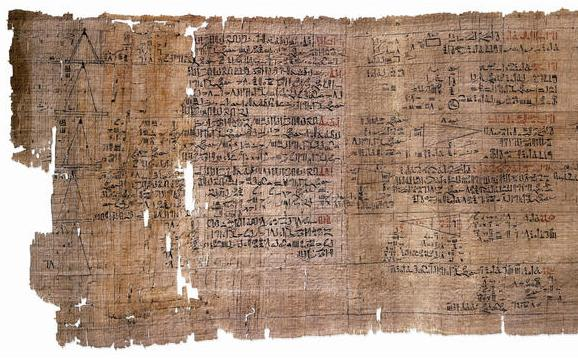
\includegraphics{Rhind_Mathematical_Papyrus.jpg}
A fragment of the Rhind papyrus, 1650BCE, containing ancient Egyptian calculations using rational numbers}\SubIndex{papyrus!Rhind}\SubIndex{Rhind papyrus}

\epigraph[author={Les Dawson}]{There is a remote tribe that worships the number zero. Is nothing sacred?}\SubIndex{Dawson, Les}

\section{Rational numbers}

A \emph{rational number}\define{rational!number}\define{number!rational} is a ratio of two integers, like
\[
\frac{2}{3}, \quad \frac{-7}{9}, \quad \frac{22}{-11}, \quad \frac{0}{2}.
\]
We also write them \(2/3, -7/9, 22/{-11}, 0/2\).
In writing \(\frac{2}{3}\), the number \(2\) is the \emph{numerator}\define{numerator}, and \(3\) is the \emph{denominator}\define{denominator}.
We can think of rational numbers two different ways: 
\begin{enumerate}
\item
Geometry: Divide up an interval of length \(b\) into \(c\) equal pieces.
Each piece has length \(b/c\).
\item
Algebra: a rational number \(b/c\) is just a formal expression we write down, with two integers \(b\) and \(c\), in which \(c\ne 0\).
We agree that any rational number \(\frac{b}{c}\) is equal to \(\frac{ab}{ac}\) for any integer \(a \ne 0\).
\end{enumerate} 
Of course, the two ideas give the same objects, but in these notes, the algebra approach is best.
For example, we see that \(22/11=14/7\), because I can factor out:
\[
\frac{22}{11} = \frac{11 \cdot 2}{11 \cdot 1},
\]
and factor out
\[
\frac{14}{7} = \frac{7 \cdot 2}{7 \cdot 1}.
\]
Write any rational number \(\frac{b}{1}\) as simply \(b\), and in this way see the integers sitting among the rational numbers.

More generally, any rational number \(b/c\) can be simplified by dividing \(b\) and \(c\) by their greatest common divisor, and then changing the sign of \(b\) and of \(c\) if needed, to ensure that \(c > 0\); the resulting rational number is \emph{in lowest terms}.

\begin{problem}{rationals:lowest.terms}
Bring these rational numbers to lowest terms: \(224/82\), \(324/-72\), \(-\num{1000}/\num{8800}\).
\end{problem}
\begin{answer}{rationals:lowest.terms}
\(224/82=112/41\), \(324/-72=-9/2\), \(-\num{1000}/\num{8800}=-5/44\).
\end{answer}

Multiply rational numbers by
\[
\frac{b}{c} \frac{B}{C} = \frac{bB}{cC}.
\]
Similarly, divide a rational number by a \emph{nonzero} rational number as
\[
\frac{\frac{b}{c}}{\frac{B}{C}} = \frac{b}{c} \frac{C}{B}.
\]
Add rationals with the \emph{same denominator} as:
\[
\frac{b}{d} + \frac{c}{d} = \frac{b+c}{d}.
\]
The same for subtraction:
\[
\frac{b}{d} - \frac{c}{d} = \frac{b-c}{d}.
\]
But if the denominators don't match up, we rescale to make them match up:
\[
\frac{b}{c} + \frac{B}{C} = \frac{bC}{cC} + \frac{cB}{cC}.
\]

\begin{problem}{rationals:define.ops}
If we replace \(\frac{b}{c}\) by \(\frac{ab}{ac}\) and we replace \(\frac{B}{C}\) by \(\frac{AB}{AC}\), for some nonzero integers \(a,A\), prove that the result of computing out \(\frac{b}{c}+\frac{B}{C}\), \(\frac{b}{c}-\frac{B}{C}\) or \(\frac{b}{c}\frac{B}{C}\) only changes by scaling both numerator and denominator by the same nonzero integer.
Hence the arithmetic operations don't contradict our agreement that we declare \(\frac{b}{c}\) to equal \(\frac{ab}{ac}\).
\end{problem}
\begin{answer}{rationals:define.ops}
We can start by defining, for any pair of integers \((b,c)\) with \(c \ne 0\), and any pair of integers \((B,C)\) with \(C \ne 0\), a rational number  
\[
\frac{\beta}{\gamma}=(Cb+cB,cC).
\]
This is well defined, since \(cC \ne 0\).
If we replace \((b,c)\) by \((ab,ac)\) and replace \((B,C)\) by \((AB,AC)\), then we get rational number
\[
\frac{ACab+acAB}{acAC}=\frac{(Aa)(Cb+cB)}{(Aa)(Cc)}=\frac{Cb+cB}{Cc}
\]
unchanged.
So the resulting \(\beta/\gamma\) is independent of the choices of pairs, depending only on the rational numbers \(b/c\) and \(B/C\).
The other proofs are very similar.
\end{answer}

\begin{problem}{rationals:arithmetic}
By hand, showing your work, simplify
\[
\frac{2}{3}-\frac{1}{2}, \frac{324}{49} \cdot \frac{392}{81},
\frac{4}{5}+\frac{7}{4}.
\]
\end{problem}
\begin{answer}{rationals:arithmetic}
By hand, showing your work, simplify
\[
\frac{2}{3}-\frac{1}{2}=\frac{1}{6}, \frac{324}{49} \cdot \frac{392}{81}=32,
\frac{4}{5}+\frac{7}{4}=\frac{51}{20}.
\]
\end{answer}

\begin{lemma}
The number \(\sqrt{2}\) is irrational.
(To be more precise, no rational number squares to \(2\).)
\end{lemma}
\begin{proof}
If it is rational, say \(\sqrt{2}=\frac{b}{c}\), then \(c \sqrt{2}=b\), so squaring gives \(c^2 \cdot 2 = b^2\).
Every prime factor in \(b\) occurs twice in \(b^2\), so the prime factorization of the right hand side has an even number of factors of each prime.
But the left hand side has an odd number of factors of \(2\), since \(c^2\) has an even number, but there is another factor of \(2\) on the left hand side.
This contradicts uniqueness of prime factorization.
\end{proof}

\begin{problem}{rationals:square.roots}
Suppose that \(N\) is a positive integer.
Prove that either \(\sqrt{N}\) is irrational or \(N\) is a \emph{perfect square}\define{perfect square}, i.e. \(N=n^2\) for some integer \(n\).
\end{problem}

\begin{problem}{rationals:square.roots.2}
Prove that there are no rational numbers \(x\) and \(y\) satisfying \(\sqrt{3}=x+y\sqrt{2}\).
\end{problem}
\begin{answer}{rationals:square.roots.2}
If \(\sqrt{3}=x+y\sqrt{2}\), square both sides to get
\[
3 = x^2+2xy\sqrt{2}+2y^2.
\]
If \(y\ne 0\), we can solve for \(\sqrt{2}\) as a rational expression in \(x,y\), so a rational number, a contradiction.
Hence \(y=0\) and \(\sqrt{3}=x\) is rational, a contradiction.
\end{answer}


A rational number is \emph{positive}\define{positive!rational number} if it is a ratio of positive integers.
We write \(x > y\) to mean that \(x-y\) is positive, and similarly define \(x<y\), \(x\le y\), and so on.

\begin{problem}{rationals:factorization}
Prove that every positive rational number has a unique expression in the form
\[
\frac{p_1^{\alpha_1} p_2^{\alpha_2} \dots p_k^{\alpha_k}}%
{q_1^{\beta_1} q_2^{\beta_2} \dots q_{\ell}^{\beta_{\ell}}}
\]
where
\[
p_1, p_2, \dots, p_k, q_1, q_2, \dots, q_{\ell}
\] 
are prime numbers, all different, with \(p_1 < p_2 < \dots < p_k\) and \(q_1 < q_2 < \dots < q_{\ell}\) and
\[
\alpha_1, \alpha_2, \dots, \alpha_k,
\beta_1, \beta_2, \dots, \beta_{\ell}
\]
are positive integers.
For example
\[
\frac{234}{16}=\frac{3^2 \cdot 13}{2^3}.
\]
\end{problem}
\begin{answer}{rationals:factorization}
By definition, every positive rational number is a ratio \(b/c\) with \(b\) and \(c\) positive.
We can divide out their greatest common divisor to arrange that \(b,c\) are coprime.
Take the prime factorization of \(b\), and that of \(c\).
As they are coprime, no prime occurs in both factorizations. 
\end{answer}

\begin{problem}{rationals:properties}
Of the various laws of addition and multiplication and signs for integers, which hold true also for rational numbers?
\end{problem}

The most important property that rational numbers have, that integers don't, is that we can divide any rational number by any nonzero rational number.



\section{Real numbers}

\epigraph[author={J.A.~Froude}]{Order is an exotic in Ireland. It has been imported from England but will not grow. It suits neither soil nor climate.}

Think of the rational numbers geometrically, so that \(b/c\) is the length of each piece when a rod of length \(b\) is cut into \(c\) equal lengths.
Draw an straight line, infinite in both directions, and mark a point \(0\) on it.
Then mark at point \(1\) at 1 unit of distance from \(0\), and so on marking all of the integers to form a \emph{number line}.\define{number line}
The points of this continuous number line are the \emph{real numbers}.
This physical definition doesn't make it possible to prove anything about the real numbers.

The rational numbers are insufficient for algebra: they have no \(\sqrt{2}\).
Imagine taking all positive rational numbers \(b/c\) for which \(b^2/c^2 > 2\).
Thinking geometrically, drawing a number line:
\begin{center}
\begin{tikzpicture}
\draw[gray](-1,0) -- (3,0);
\draw[thick]({sqrt(2)},0) -- (3,0);
\fill[white,draw=black] ({sqrt(2)},0) circle (1.2pt);
\node[below] at ({sqrt(2)},0) {\(\sqrt{2}\)};
\end{tikzpicture}
\end{center}
Our rational numbers sit along the line getting very close to the circled point of the line, which should be the point \(\sqrt{2}\).
But there is no rational number there.
From now on, we assume that the reader is familiar with the real numbers and their basic properties; see \cite{Spivak:2006} for the complete story of real numbers.


\section{Complex numbers}
\epigraph[author={Paul Painlev\'e}, source={Analyse des travaux scientifiques}, translation={The shortest and easiest path between any two facts about the real domain often passes through the complex domain.}]{Entre deux vérités du domaine réel, le chemin le plus facile et le plus court passe bien souvent par le domaine complexe.}%
\SubIndex{Painlev\'e, Paul}
Just as the rational numbers have a deficiency, no \(\sqrt{2}\), so the real numbers have a deficiency: no \(\sqrt{-1}\).
We can fix this by introducing the complex numbers.
Here are two definitions:
\begin{enumerate}
\item
\emph{Algebra:} We agree to play a game, where we write down algebraic expressions in real numbers and in an abstract variable \(i\), but we treat the symbol \(i\) according to the following rule.
Whenever we see two copies of \(i\) multiplied together (or we see \(i^2\)) appear anywhere, we are allowed to wipe them out and replace with \(-1\), and vice versa when we see a \(-1\) we can replace it with an \(i^2\).
We force by hand the existence of a \(\sqrt{-1}\) by forcing the abstract symbol \(i\) to be \(\sqrt{-1}\).
\item
\emph{Geometry:} We draw the usual \(x,y\) axes on the plane.
We pretend that each point of the plane represents a single number, which we write as \(z=x+yi\) to represent the point \((x,y)\).
If we have two points, \(z=x+yi\) and \(Z=X+Yi\), we add them by the rule:
\[
z+Z=(x+X)+(y+Y)i
\]
and multiply them by the rule:
\[
zZ=(xX-yY)+(xY+yX)i.
\]
For example, 
\[
(2+4i)(3-i)=(2\cdot 3 + 4\cdot 1)+(-2+4\cdot 3)i=10+10i.
\]
\end{enumerate}
It isn't at all clear that these two games we can play arrive at the same result.
Note that the rule for multiplication seems to come out of the air in the geometric theory, but in the algebraic theory it is just what you get by expanding out both sides and insisting that \(i^2=-1\).
Algebra is in this respect clearly superior. 
But the geometric approach makes very precise what sort of objects we are really dealing with, so we will use it as our definition.

Just like with rational numbers, if a complex number \(z=x+yi\) is not zero, or in other words \(x\) and \(y\) are not both zero, then it has a reciprocal
\[
\frac{1}{z} = \frac{x-yi}{x^2+y^2}.
\]
\begin{problem}{rationals:recip.c}
Check that this is a reciprocal.
Why is it defined?
\end{problem}


\emph{Complex conjugation}\define{complex conjugation} is the operation taking \(z=x+yi\) to \(\bar{z}\defeq x-iy\).
\begin{problem}{rationals:conjugate.real}
Prove that a complex number \(z\) is a real number just when \(z=\bar{z}\). 
\end{problem}
\begin{problem}{rationals:conjugate}
Prove that addition, subtraction, multiplication and division of complex numbers passes through conjugation:
\begin{align*}
\overline{z+w}&=\bar{z}+\bar{w}, \\
\overline{z-w}&=\bar{z}-\bar{w}, \\
\overline{zw}&=\bar{z} \, \bar{w}, \\
\overline{\pr{\frac{z}{w}}}&=\frac{\bar{z}}{\bar{w}},
\end{align*}
for any complex numbers \(z\) and \(w\).
Explain by induction why, for any polynomial \(p(z)\) with real number coefficients,
\[
\overline{p(z)}=p\of{\bar{z}},
\]
for any complex number \(z\).
\end{problem}

The \emph{norm}\define{norm} or \emph{modulus}\define{modulus} of a complex number \(z=x+yi\) is the real number \(|z|\defeq\sqrt{x^2+y^2}\)\Notation{(z)}{\lengthForNotationIndex{z}}{modulus of a complex number}.

\begin{problem}{rationals:norm}
Prove that \(z\bar{z}=|z|\) for any complex number \(z\).
\end{problem}


\section{Sage}

Sage represents numbers in two different ways: as exact symbolic expressions, or as a finite decimal approximation (often called a \emph{numeric} or \emph{floating point} representation). 
For example we compute \(\frac{7}{2}+\frac{5}{3}\) symbolically as
\begin{sageblock}
7/2+5/3
\end{sageblock}
yielding \(\sage{7/2+5/3}\).
We can also play with irrational numbers symbolically: represent \(\sqrt{27}\) as
\begin{sageblock}
sqrt(27)
\end{sageblock}
which sage simplifies to yield \(\sage{sqrt(27)}\).

We will \emph{never} use decimal approximations in this class (please don't), but here is how you can use them if you wish.
By writing out a number with a decimal point, we are asking sage to approximate numerically, keeping only some number of decimals accuracy:
\begin{sageblock}
sqrt(27.0)
\end{sageblock}
yields \(\sage{sqrt(27.0)}\).
If we want to ask sage to give us a particular number of decimal places accuracy in a decimal approximation of a symbolic expression, say \(50\) decimals:
\begin{sageblock}
numerical_approx(pi, digits=50)
\end{sageblock}
yields 
\[
\sage{numerical_approx(pi, digits=50)}.
\]

To use complex numbers, try 
\begin{sageblock}
z=3+4*i
real_part(z)
\end{sageblock}
yielding \(3\), the real part, while \verb!imag_part(z)! yields \(4\).



\chapter{Polynomials}
\epigraph[author={Augustus De Morgan (when asked his age)}]{I was \(x\) years old in the year \(x^2\).}\SubIndex{De Morgan, Augustus}
A \emph{polynomial}\define{polynomial} in a variable \(x\) is an expression like
\[
1, x+1, 5+3x^2-2x.
\]
Let us be more precise.
\begin{center}
\begingroup
\tikzstyle{every picture}+=[remember picture]
\tikzstyle{na} = [baseline=-.5ex]
\tikz[na] \draw node[fill=blue!20] (n1) {coefficient};
\tikz[na] \draw node[fill=red!20] (n2) {variable};
\tikz[na] \node[fill=green!20] (n3) {degree};

\medskip

\qquad\qquad\qquad
\(
        \tikz[baseline]{
            \node[inner sep=1pt,fill=blue!20,anchor=base] (t1)
            {$75$};
        }
        \tikz[baseline]{
            \node[inner sep=1pt,fill=red!20, %ellipse,
            anchor=base] (t2)
            {$x$};
        }
        \tikz[baseline]{
            \node[inner sep=0pt,fill=green!20,anchor=base] (t3)
            {${}^{18}$};
        }
\)
\begin{tikzpicture}[overlay]
        \path[-stealth] (n1) edge [bend right] (t1);
        \path[-stealth] (n2) edge (t2);
        \path[-stealth] (n3) edge [bend left] (t3);
\end{tikzpicture}
\endgroup
\end{center}
A \emph{monomial}\define{monomial} in a variable \(x\) is the product of a number (the \emph{coefficient}\define{coefficient!of polynomial} of the term) with a nonnegative integer power of \(x\) (the \emph{degree} of the term).
Write \(x^1\) as \(x\).
Write \(x^0\) as \(1\), and so write any monomial of degree zero as just its coefficient, and call it a \emph{constant}.
If the coefficient of a monomial is \(1\), write it without a coefficient: \(1 \, x^{57}=x^{57}\).

A \emph{polynomial} is a finite sum of monomials, its \emph{terms}.\define{term}
We can write the sum in any order, and drop any terms with zero coefficient, without changing the polynomial.
If the sum has no terms, write the polynomial as \(0\).
A \emph{constant} is a polynomial which has only a constant term or is \(0\).
Add polynomials by adding coefficients of terms of the same degree:
\[
2x^2+7x^2+x=(2+7)x^2+x=9x^2+x.
\]
Hence we can write any polynomial so that all terms have different degree, say decreasing in degree, or increasing in degree: \(1+x^3+5x=1+5x+x^3=x^3+5x+1\), and drop all terms with zero coefficient.
Two polynomials written this way are equal just when they have the same coefficient in every degree.
The \emph{degree}\define{degree!of polynomial} is the largest degree of any term.
The degree of \(0\) is defined to be \(-\infty\).
Multiply monomials like \((7x^2)(5x^3)=(7 \cdot 5)x^{2+3}\), multiplying coefficients and adding degrees.
Multiply polynomials by the distributive law, term by term.
The coefficients can be integers, rational numbers, real numbers, or complex numbers (in which case, we usually use \(z\) as the name of the variable, instead of \(x\)).
They can even be remainders modulo some integer.
As soon as we fix our choice of coefficients, the addition laws, multiplication laws, and distributive law (familiar from chapter~\ref{chapter:integers}) follow: write \(b(x)\) as a polynomial, instead of an integer \(b\), and so on, and change the word \emph{integer} to \emph{polynomial}.
Ignore the sign laws and the law of well ordering.
\begin{example}
Let's work modulo \(2\), in honour of George Boole.
Let \(p(x)\defeq x^2+x\).
We write \(x^2+x\) to mean \(\bar{1} x^2 + \bar{1} x\), i.e. the coefficients are remainders.
This polynomial is not zero, because its coefficients are not zero.
\emph{Danger:} we might want to think of this polynomial as a \emph{function} of a variable \(x\), and ask that \(x\) also be a remainder modulo \(2\).
But then that function \emph{is} zero, because if we let \(x=\bar{0}\) then
\[
p\of{\bar{0}}=\bar{1}\cdot\bar{0}^2+\bar{1}\cdot\bar{0}=\bar{0}
\]
and if we let \(x=\bar{1}\) then
\[
p\of{\bar{1}}=\bar{1}\cdot\bar{1}^2+\bar{1}\cdot\bar{1}=\bar{0}
\]
modulo \(2\).
So a polynomial is \emph{not} just a function: the function can be zero while the polynomial is not.
A polynomial is a purely algebraic object.
\end{example}
\begin{problem}{polynomials:squares}
Work modulo \(5\): for which remainders \(a\) can we find a remainder \(b\) so that \(a=b^2\)?
In other words, which elements have square roots?
\end{problem}
\begin{problem}{polynomials:int.values}
Give an example of a polynomial \(b(x)\) none of whose coefficients are integers, so that, if we set \(x\) to an integer value, then \(b(x)\) takes an integer value.
\end{problem}
\begin{answer}{polynomials:int.values}
Take the polynomial \(b(x)=(1/2)x(x+1)=(1/2)x^2+(1/2)x\).
If \(x\) is an odd integer, then \(x+1\) is even, and vice versa, so \(b(x)\) is an integer for any integer \(x\).
\end{answer}

\section{The extended Euclidean algorithm}
You are familiar with long division of polynomials.
For example, to divide \(x-4\) into \(x^4-3x+5\), we have to order the terms in decreasing degrees as usual, and add in zero terms to get all degrees to show up then\label{equation:extended.Euclid.example}
\[
\begin{array}{@{}rr@{}r@{}r@{}r@{}r@{}}
    & x^3 & +4x^2 & +16x  & +61 \\
     \cmidrule{2-6} 
x-4 & x^4 & +0x^3 & +0x^2 & -3x & +5 \\
    & x^4 & -4x^3 \\
    \cmidrule{2-6}
    &     &  4x^3 & +0x^2 & -3x & +5 \\
    &     &  4x^3 & -16x^2 \\
    \cmidrule{3-6}
    &     &       & 16x^2 & -3x & +5 \\
    &     &       & 16x^2 & -64x \\
    \cmidrule{4-6}
    &     &       &       & 61x & +5\\
    &     &       &       & 61x & -244 \\
    \cmidrule{5-6}
    &     &       &       &     &  249    
\end{array}
\]
The quotient is \(x^3+4x^2+16x+61\) and the remainder is \(249\).
Summing up, this calculation tells us that
\[
x^4-3x+5 = (x-4) \pr{x^3+4x^2+16x+61} + 249,
\]
We stop when the remainder has small \emph{degree} than the expression we want to divide in, in this case when \(249\) has degree zero, smaller than the degree of \(x-4\).

In this simple problem, we never needed to divide.
But in general, to divide \(b(x)\) by \(c(x)\), we might need to divide coefficients of \(b(x)\) by those of \(c(x)\) at some stage.
Therefore from now on, we will restrict the choice of coefficients to ensure that we can always divide.
For example, we can carry out long division of any two polynomials with rational coefficients, and we always end up with a quotient and a remainder, which are themselves polynomials with rational coefficients.
The same is true if we work with real number coefficients, or complex number coefficients.
But if we work with integer coefficients, the resulting quotient and remainder might only have rational coefficients.
\begin{problem}{polynomials:B\'ezout}
Determine the greatest common divisor of \(b(x) = x^3 +4x^2+x-6\) and \(c(x) = x^5-6x+5\) and the associated B\'ezout coefficients \(s(x), t(x)\).
\end{problem}
It is trickier to specify the restrictions on coefficients if they are to be remainders modulo an integer.
From now on, we will only work with remainders modulo a prime.
The reason is that every nonzero remainder modulo a prime has a reciprocal, so we can always divide coefficients.
\begin{problem}{polynomials:prime.field}
Prove that every nonzero remainder modulo a prime has a reciprocal modulo that prime.
\end{problem}
With these restrictions on coefficients, we can immediately generalize the Euclidean and extended Euclidean algorithms, and compute B\'ezout coefficients and least common multiples, using the same proofs, so we won't repeat them.
\begin{example}
Take the polynomials \(b(x)=3+2x-x^2\) and \(c(x)=12-x-x^2\).
We want to find the B\'ezout coefficients and the greatest common divisor among polynomials over the rational numbers.
At each step, force down the degree of one of the polynomials.
\begin{align*}
& \begin{pmatrix}
    1 & 0 & 3+2x-x^2 \\
    0 & 1 & 12-x-x^2
  \end{pmatrix} \text{ add -row 2 to row 1}, 
  \\
& \begin{pmatrix}
    1 & -1 & -9+3x\\
    0 & 1 & 12-x-x^2
  \end{pmatrix} \text{ add \((x/3)\)row 1 to row 2}, 
  \\
& \begin{pmatrix}
    1 & -1 & -9+3x \\
    \frac{x}{3} & 1-\frac{x}{3} & 12-4x
  \end{pmatrix} \text{ add } \frac{4}{3}\text{row 1 to row 2}, 
  \\
& \begin{pmatrix}
    1 & -1 & -9+3x \\
    \frac{4}{3}+\frac{x}{3} & -\frac{1}{3}-\frac{x}{3} & 0
  \end{pmatrix}
\end{align*}
The equation of the B\'ezout coefficients is therefore
\[
1\pr{3+2x-x^2} -1\pr{12-x-x^2} = -9+3x = 3(x-3).
\]
The greatest common divisor, once we divide away any coefficient in front of the highest term, is \(x-3\).
A \emph{monic polynomial}\define{monic polynomial}\define{polynomial!monic} is one whose highest degree term has coefficient \(1\): the greatest common divisor will always be taken to be a monic polynomial, and then there is a unique greatest common divisor.
\end{example}
Fix a choice of whether we are working with rational, real or complex coefficients or if our coefficients will be remainders modulo a prime.
We will say this choice is a choice of \emph{field}\define{field}, and our polynomials are said to live \emph{over} that field.
A polynomial over a chosen field is \emph{irreducible}%
\define{irreducible!polynomial}%
\define{reducible!polynomial}% 
\define{polynomial!irreducible}%
\define{polynomial!reducible}
if it does not split into a product \(a(x)b(x)\) of polynomials over the same field, except for having \(a(x)\) or \(b(x)\) constant.
The same proof for prime numbers proves that a polynomial over a field admits a factorization into a product of irreducibles over that field, unique up to reordering the factors and perhaps multiplying any of the factors by a nonzero constant.
\begin{example}
Let's working over the remainders modulo 2.
Notice that \(2x=0x=0\), and similarly that \(-1=1\) so \(-x^2=x^2\).
Let's find the B\'ezout coefficients of \(b(x)\defeq x^3+x\) and \(c(x)\defeq x^2\):
\begin{align*}
&  \begin{pmatrix}
  1 & 0 & x^3 + x \\
  0 & 1 & x^2
  \end{pmatrix}, \text{ add } x\text{(row 2) to row 1},
  \\
&  \begin{pmatrix}
  1 & x & x \\
  0 & 1 & x^2
  \end{pmatrix}, \text{ add } x\text{(row 1) to row 2},
  \\
&  \begin{pmatrix}
  1 & x & x \\
  x & x^2+1 & 0
  \end{pmatrix}. 
\end{align*}
The B\'ezout coefficients are \(1, x\), and the greatest common divisor is \(x\):
\[
1\pr{x^3+x} + x\pr{x^2} = x.
\]
\end{example}
\begin{problem}{polynomials:Bezout.mod.3}
Find the B\`ezout coefficients of \(b(x)=x^3+x\), \(c(x)=x^4+1\) with coefficients in remainders modulo 3.
\end{problem}
\begin{answer}{polynomials:Bezout.mod.3}
Keep in mind that, modulo \(3\), \(-1=2,-2=1\), \(1^{-1}=1\), \(2^{-1}=2\), so
\begin{align*}
&
\begin{pmatrix}
1 & 0 & x^3+x \\
0 & 1 & x^4+1
\end{pmatrix} \text{ add \(-x\)(row 1) to row 2},
\\
&
\begin{pmatrix}
1 & 0 & x^3+x \\
-x & 1 & -x^2+1
\end{pmatrix} \text{ add \(x\)(row 2) to row 1},
\\
&
\begin{pmatrix}
1-x^2 & x & 2x \\
-x & 1 & -x^2+1
\end{pmatrix} \text{ add \(2x\)(row 1) to row 2},
\\
&
\begin{pmatrix}
1-x^2 & x & 2x \\
x^3+x & 1+2x^2 & 1
\end{pmatrix}
\end{align*}
So the B\'ezout coefficients are \(x^3+x,1+2x^2\) and the gcd is \(1\).
We can check: expand out
\[
(x^3+x)(x^3+x)+(1+2x^2)(x^4+1)=(x^6+2x^4+x^2)+(2x^6+x^4+2x^2+1)=1.
\]
\end{answer}




\section{Factoring}
\epigraph[author={A. A. Kirillov}, source={What are Numbers?}]
{{}-{} What is a multiple root of a polynomial? \\
{}-{} Well, it is when we substitute a number in the polynomial and get zero. Then do it again and again
get zero and so \(k\) times \dots. But on the \((k+1)\)-st time the zero does not appear.}\SubIndex{Kirillov, A. A.}
\begin{proposition}
Take any constant \(c\) and any polynomial \(p(x)\) over any field.
Then \(p(x)\) has remainder \(p(c)\) when divided by \(x-c\).
\end{proposition}
\begin{proof}
Take quotient and remainder: \(p(x)=(x-c)q(x)+r(x)\), using the Euclidean algorithm.
The degree of the remainder is smaller than the degree of \(x-c\), so the remainder is a constant, say \(r_0\).
Plug in \(x=c\): \(p(c)=(c-c)q(c)+r_0=r_0\).
\end{proof}
A \emph{root} of a polynomial \(p(x)\) is a number \(c\) in whichever field we work over so that \(p(c)=0\).
\begin{corollary}\label{corollary:divide.poly}
A polynomial \(p(x)\) over any field has a root at \(x=c\), i.e. \(p(c)=0\), for some constant \(c\) in the field, just when the linear polynomial \(x-c\) divides into \(p(x)\).
\end{corollary}
\begin{problem}{polynomials:sqrts}
Over the field of real numbers, or the field of rational numbers, or the field of complex numbers, or the field of remainders modulo any odd prime number: show that every constant \(d\) has either two square roots, which we denote as \(\pm \sqrt{d}\), or one square root (if \(2=0\) in our field or if \(d=0\)) or has no square roots.
\end{problem}
\begin{problem}{polynomials:quadratic.formula}
Work over the field of real numbers, or the field of rational numbers, or the field of complex numbers, or the field of remainders modulo any odd prime number.
Show that the solutions of the quadratic equation
\[
0 = ax^2 + bx + c
\]
(where \(a, b, c\) are constants and \(a \ne 0\)) are precisely the numbers \(x\) so that
\[
\pr{x+\frac{b}{2a}}^2 = \frac{b^2}{2a^2}-\frac{c}{a}.
\]
Prove that the solutions of the quadratic equation, over any field, are
\[
x=\frac{-b\pm\sqrt{b^2-4ac}}{2a}.
\]
just when the required square roots exist.
\end{problem}
\begin{problem}{polynomials:factor.quadratic}
Prove that a quadratic\define{quadratic!polynomial}\define{polynomial!quadratic} or cubic\define{cubic!polynomial}\define{polynomial!cubic} polynomial (in other words of degree 2 or 3) over any field is reducible just when it has a root.
\end{problem}
\begin{problem}{polynomials:find.root.binary}
Prove that the polynomial \(x^3+x+1\) is irreducible over the field of remainders modulo \(2\).
By writing down all quadratic polynomials over that field, and factoring all of them but this one, show that this is the only irreducible quadratic polynomial over that field.
\end{problem}
\begin{example}
The polynomial \(x^3+x+1\) is irreducible over the field of remainders modulo \(2\), as we saw in the previous problem.
But then, if it is reducible over the integers, say \(a(x)b(x)\), then quotient out the coefficients modulo \(2\) to get a factorization \(\bar{a}(x)\bar{b}(x)\) over the field of remainders modulo \(2\), a contradiction.
Therefore \(x^3+x+1\) is irreducible over the integers.  
\end{example}
\begin{corollary}
Every polynomial over any field has at most one factorisation into linear factors, up to reordering the factors.
\end{corollary}
\begin{proof}
The linear factors are determined by the roots.
Divide off one linear factor from each root, and apply induction on the degree of the polynomial to see that the number of times each linear factor appears is uniquely determined.
\end{proof}
\begin{problem}{polynomials:roots.determine}
Suppose that \(p(x)\) and \(q(x)\) are polynomials over some field, both of degree at most \(n\), and that \(p(c)=q(c)\) for \(n+1\) different numbers \(c\) from the field.
Prove that \(p(c)=q(c)\) for all numbers \(c\) from the field.
\end{problem}
\begin{problem}{polynomials:not.prime.characteristic}
Why are we working over fields?
Working modulo \(6\), consider the polynomial \(b(x)=x^2+5x\).
How many roots does it have among the remainders module \(6\)?
How many factorizations can you make for it, working modulo \(6\)?
\end{problem}
\begin{answer}{polynomials:not.prime.characteristic}
roots: 0, 1, 3, 4; factorizations: \((x+2)(x+3)=x(x+5)\).
\end{answer}
A root \(c\) of a polynomial \(p(x)\) has \emph{multiplicity \(k\)} if \((x-c)^k\) divides \(p(x)\).
\begin{corollary}
Over any field, the degree of a polynomial is never less than the sum of the multiplicities of its roots, with equality just when the polynomial is a product of linear factors.
\end{corollary}
\begin{proof}
Degrees add when polynomials multiply, by looking at the leading term.
\end{proof}

\section{Rational roots}
A powerful trick for guessing rational roots of integer coefficient polynomials:
\begin{lemma}\label{lemma:guess.roots}
If a polynomial \(p(x)\) with integer coefficients has a rational root \(x=n/d\), with \(n\) and \(d\) coprime integers, then the numerator \(n\) divides the coefficient of the lowest term of \(p(x)\), while the denominator \(d\) divides the coefficient of the highest term of \(p(x)\).
\end{lemma}
\begin{proof}
Write out 
\[
p(x)=a_k x^k + a_{k-1} x^{k-1} + \dots + a_1 x + a_0,
\]
so that these integers \(a_0, a_1, \dots, a_k\) are the coefficients of \(p(x)\).
Plug in:
\[
0 = a_k (n/d)^k + a_{k-1} (n/d)^{k-1} + \dots + a_1 (n/d) + a_0.
\]
Multiply both sides by \(d^k\):
\[
0 = a_k n^k + a_{k-1} n^{k-1} d  + \dots + a_1 n d^{k-1} + a_0 d^k.
\]
All terms but the last term contain a factor of \(n\), so \(n\) divides into the last term.
But \(n\) and \(d\) are coprime, so \(n\) divides into \(a_0\).
The same trick backwards: all terms but the first term contain a factor of \(d\), so \(d\) divides into the first term.
But \(n\) and \(d\) are coprime, so \(d\) divides into \(a_k\).
\end{proof}
\begin{example}\label{example:x.cubed}
The polynomial \(p(x)=x^3-3x-1\), if it had a rational root \(n/d\), would need to have \(n\) divide into \(-1\), while \(d\) would divide into \(1\).
So the only possibilities are \(n/d=1\) or \(n/d=-1\).
Plug in to see that these are not roots, so \(x^3-3x-1\) has no rational roots.
\end{example}
\begin{problem}{polynomials:rat.roots}
Using lemma~\vref{lemma:guess.roots}, find all rational roots of 
\begin{enumerate}
\item
\(x^2-5\),
\item
\(x^2-3x-5\),
\item
\(x^{1000}-3x-5\).
\item
\(x^2/3-x-5/3\),
\end{enumerate}
\end{problem}



\section{Sage}
\epigraph[author={Norbert Wiener}, source={The Human Use Of Human Beings: Cybernetics And Society}]{The world of the future will be an even more demanding struggle against the limitations of our intelligence, not a comfortable hammock in which we can lie down to be waited upon by our robot slaves.}\SubIndex{Wiener, Norbert}\SubIndex{The Human Use Of Human Beings: Cybernetics And Society}%
To construct polynomials in a variable \(x\), we first define the variable, using the strange expression:
\begin{sageblock}
x = var('x')
\end{sageblock}
We can then solve polynomial equations:
\begin{sageblock}
solve(x^2 + 3*x + 2, x)
\end{sageblock}
yielding \verb![x == -2, x == -1]!.
To factor polynomials:
\begin{sageblock}
x=var('x')
factor(x^2-1)
\end{sageblock}
yields \verb!(x + 1)*(x - 1)!.
To use two variables \(x\) and \(y\):
\begin{sageblock}
x, y = var('x, y')
solve([x+y==6, x-y==4], x, y)
\end{sageblock}
yielding \verb![[x == 5, y == 1]]!.
We can take greatest common divisor:
\begin{sageblock}
x=var('x')
b=x^3+x^2
c=x^2+x
gcd(b,c)
\end{sageblock}
yielding \(\sage{gcd(b,c)}\).
For some purposes, we will need to tell sage which field the coefficients of our polynomials come from.
We can get the quotient and remainder in polynomial division by
\begin{sageblock}
R.<x> = PolynomialRing(QQ)
b=x^3+x^2
c=x^2+x
b.quo_rem(c)
\end{sageblock}
yielding \(\sage{b.quo_rem(c)}\).
To find B\'ezout coefficients, 
\begin{sageblock}
xgcd(x^4-x^2,x^3-x)
\end{sageblock}
yields \(\sage{xgcd(x^4-x^2,x^3-x)}\).

The expression \verb!R.<x> = PolynomialRing(QQ)! tells sage to use polynomials in a variable \(x\) with coefficients being rational numbers. The set of all rational numbers is called \(\Q{}\), written \verb!QQ! when we type into a computer.
To work with coefficients that are integers modulo a prime, for example with integers modulo \(5\):
\begin{sageblock}
R.<x> = PolynomialRing(GF(5))
b=x^3+x^2+1
c=x^2+x+1
b.quo_rem(c)
\end{sageblock}
yields \(\sage{b.quo_rem(c)}\).
The set of all integers modulo a prime \(p\) is sometimes called \(\operatorname{GF}(p)\).

We can define our own function to calculate B\'ezout coefficients, which does exactly what the \verb!xgcd()! function does on polynomials of one variable:
\begin{sageblock}
def bezpoly(b,c):
    p,q,r=1,0,b
    s,t,u=0,1,c
    while u<>0:
        if r.degree()>u.degree():
            p,q,r,s,t,u=s,t,u,p,q,r
        Q=u//r
        s,t,u=s-Q*p,t-Q*q,u-Q*r
    return (r,p,q)
\end{sageblock}
Then the code
\begin{sageblock}
R.<t> = PolynomialRing(QQ)
f=(2*t+1)*(t+1)*(t-1)
g=(2*t+1)*(t-1)*t^2
bezpoly(f,g)
\end{sageblock}
returns
\(\sage{bezpoly(f,g)}\).


\section{Interpolation}
\epigraph[author={Henri Poincar\'e}, source={La Science et L'Hypoth\`ese},translation={Analyse data just so far as to obtain simplicity and no further.}]{Il faut bien s'arr\^eter quelque part, et pour que la science soit possible, il faut s'arr\^eter quand on a trouv\'e la simplicité.}\SubIndex{Poincar\'e, Henri}\SubIndex{La Science et L'Hypoth\`ese}
\begin{theorem}
Over any field, if we specify distinct values \(x_0, \dots, x_n\) and arbitrary values \(y_0, \dots, y_n\), there is a unique polynomial \(p(x)\) of degree \(n\) so that \(p(x_i)=y_i\).
\end{theorem}
The polynomial \(p(x)\) \emph{interpolates}\define{interpolation} the values \(y_i\) at the points \(x_i\).
\begin{proof}
We associate to the numbers \(x_0, \dots, x_n\) the polynomials
\[
p_j(x)=
\frac{(x-x_0)\dots(x-x_{j-1})(x-x_{j+1})\dots(x-x_n)}{(x_j-x_0)\dots(x_j-x_{j-1})(x_j-x_{j+1})\dots(x_j-x_n)}.
\]
for \(j=0,1,2,\dots,n\).
The reader can check that \(p_j(x_j)=1\) while \(p_j(x_i)=0\) for \(i \ne j\).
Then 
\[
p(x)=
y_0 p_0(x) + y_1 p_1(x) + \dots + y_n p_n(x)
\]
is our required polynomial.
To check that it is unique, if there are two such polynomials, say \(p(x)\) and \(q(x)\), both of degree at most \(n\), both equal to \(y_i\) at \(x=x_i\), their difference \(p(x)-q(x)\) vanishes at \(x=x_i\), so is divisible by \((x-x_0)(x-x_1)\dots(x-x_n)\), which has degree \(n+1\).
But their difference has degree at most \(n\), so is zero.
\end{proof}
\begin{problem}{polynomials:interpolation}
What can go wrong with interpolation if the numbers are drawn from the remainders modulo 6?
\end{problem}


\chapter{Real polynomials, complex polynomials}

In this chapter (and only this chapter), we assume that the reader is familiar with real numbers, with continuity, and with the intermediate value theorem:\define{intermediate value theorem}\define{theorem!intermediate value} every continuous function \(y=f(x)\) defined on an interval \(a \le x \le b\) takes on all values between \(f(a)\) and \(f(b)\).
We also assume that the reader knows that polynomials are continuous.
See \cite{Spivak:2006} for the complete story of continuity and the intermediate value theorem.

\section{Polynomials over the real numbers}

\begin{example}
If \(f(x)\) is a polynomial with positive coefficients, like
\[
f(x)=-4 + 7x + 17x^2 + 674x^4,
\]
then making \(x\) very large makes \(f(x)\) very large positive, clearly, since \(x^4\) eventually gets much larger than all other terms.
The equation \(f(x)=0\) must have a solution \(x>0\), because \(f(x)\) starts at \(f(0)=-4\) (negative) and then gets much larger than anything we like eventually for large enough \(x\), so gets positive, so must be zero somewhere in between.
\end{example}

\begin{problem}{rationals:cubic}
Prove that the equation
\[
394x^3-92843x^2+209374x-2830
\]
has a real number solution \(x\).
More generally, prove that any odd-order polynomial equation in a real variable has a real solution.
\end{problem}


\section{Counting positive roots}

\begin{theorem}[Descartes]\define{theorem!Descartes}\define{Descartes!theorem}
The number of positive roots, counted with multiplicities, of a real polynomial \(b(x)\) is either equal to the number of changes of sign of its coefficients (when we write the polynomial \(b(x)\) with terms in order of degree), or less by a multiple of 2.
\end{theorem}
\begin{example}
The polynomial
\[
b(x)=12x^7+x^5-x^3-x^2+x+1
\]
has coefficients with signs \(++--++\).
We ignore the zero coefficients, for example in front of \(x^6\) and \(x^4\).
So as we travel along the signs, they change twice, once from \(+\) to neighboring \(-\), and once from \(-\) to neighboring \(+\).
So this \(b(x)\) has at most \(2\) roots \(x>0\), and the number of roots with \(x>0\) is even.
So there are either 2 positive roots or none.
\end{example}
\begin{example}
The polynomial \(c(x)=x^5-3x^4+3x^3+9x^2-27x+3\) has 4 sign changes, so 4 or 2 or 0 roots \(x\) with \(x>0\).
If we look at the polynomial \(c(-x)\), expand out to get \(c(-x)=-x^5-3x^4-3x^3+9x^2+27x+3\) has 1 sign change, so 1 root with \(x>0\).
Therefore \(c(x)\) has 1 root with \(x < 0\).
\end{example}
\begin{proof}
Take a polynomial \(b(x)\).
If \(x\) divides \(b(x)\), dividing out factors of \(x\) from \(b(x)\) doesn't change positive roots or signs of coefficients, so we can assume that there are no factors of \(x\).
In other words, assume that the constant coefficient of \(b(x)\) is not zero:
\[
b(x)=b_0+b_1x+b_2x^2+\dots+b_n x^n
\] 
with \(b_0 \ne 0\) and \(b_n \ne 0\).
For large positive numbers \(x\), \(b(x)\) has the same sign as \(b_n\):
\[
\frac{b(x)}{x^n}
=
\frac{b_0}{x^n} + \frac{b_1}{x^{n-1}} + \dots + \frac{b_{n-1}}{x} + b_n \to b_n.
\]

Suppose that \(b(x)\) has no positive roots.
By the intermediate value theorem, \(b(x)\) stays that same sign for all \(x>0\).
For \(x=0\), this sign is \(b(x)=b_0\), while for \(x\) large it is the sign of \(b_n\).
So if \(b(x)\) has no roots, then \(b_0\) and \(b_n\) have the same sign, so there are an even number of sign changes, to start and end at the same sign.
In particular, the theorem is true for any polynomial \(b(x)\) with no roots.

Suppose that \(b(x)\) has a positive root, say at \(x=a\).
Factor out:
\[
b(x)=(x-a)c(x)
\]
for some polynomial \(c(x)\).
We claim that \(b(x)\) has one more sign change than \(c(x)\).
Write out the coefficients of \(c(x)\), say as
\[
c(x)=c_0+c_1x+c_2x^2+\dots+c_{n-1} x^{n-1}.
\]
Expand out the equation
\[
b(x)=(x-a)c(x)
\]
to find the relations between the coefficients:
\[
b_j = c_{j-1}-ac_j.
\]
Starting at the top, \(b_n=c_{n-1}\), the top coefficients match in sign.
As we go down the coefficients by degree, pick out the first sign change in the coefficients of \(c(x)\), say \(c_{j-1}<0\) while \(c_j>0\).
Then \(b_j=c_{j-1}-ac_j<0\), so the sign of the \(b_j\) coefficient is the same as that of \(c_{j-1}\).
If the \(b(x)\) coefficients have not already changed sign before we got to \(b_j\), then they certainly must change sign by the time we get to \(b_j\).
The same argument works for the next sign change and so on: at least as many sign changes.
Since the signs of the highest coefficients of \(b(x)\) and \(c(x)\) agree, while the signs of the lowest coefficients disagree, the total number of sign changes of \(b(x)\) must be greater than those of \(c(x)\) by an odd number: one more sign change or three more or five more, etc.

By induction, the number of positive roots of \(c(x)\) is equal to the number of sign changes of \(c(x)\) or less by a multiple of two.
Since \(b(x)\) has one more positive root, and one more sign change or three more or five more, etc., the result holds by induction on degree.
\end{proof}

\section{Sage}
The number of sign changes in a polynomial is easy to spot by eye, but we can also write sage code.
Each polynomial \verb!p! has associated list of coefficients \verb!p.list()!.
This list has the coefficients in order, but with zero entries in the list at zero coefficients.
\begin{sagesilent}
t=var('t')
p=t^5-2*t+7
\end{sagesilent}
For example, if \verb!p=t^5-2*t+7! then \verb!p.list()! yields \(\sage{p.list()}\).
We will travel along the coefficients one by one, with a for loop.
The code (which we explain below):
\begin{sageblock}
def descartes(p):
    sign = 0
    sign_changes = 0
    for c in p.list():
        if c <> 0:
            if sign == 0:
                if c < 0:
                    sign = -1
                else:
                    if c > 0:
                        sign = 1
            else:
                if c*sign < 0:
                    sign_changes = sign_changes + 1
                    sign = -sign
    return sign_changes
\end{sageblock}
We store the sign of the last nonzero coefficient in a variable \verb!sign!, which is set to zero initially to mean that we haven't yet encountered a nonzero coefficient.
If we encounter our first nonzero coefficient, we just set \verb!sign! to its value.
But if we find any subsequent nonzero coefficient, we compare whether it has the same sign as \verb!sign!, and if it has an opposite sign, i.e. if \verb!L[i]*sign<0!, then we count a new sign change.
Now calling the function:
\begin{sageblock}
t = var('t')
descartes(t^(79)-4*t^(17)+t^(10)+t^6+t-1)
\end{sageblock}
yields \(\sage{descartes(t^(79)-4*t^(17)+t^(10)+t^6+t-1)}\).




\section{Counting roots of a real polynomial in an interval}

Suppose that \(p(x)\) is a polynomial with real coefficients.
Let \(p_0(x)\) be just another name for \(p(x)\).
Let \(p_1(x)\defeq p'(x)\).
From then on, compute quotients and remainders: \(p_2(x)\) is the negative of the remainder of \(p_0(x)\) divided by \(p_1(x)\), and so on: \(p_{j+1}(x)\) is the negative of the remainder of \(p_{j-1}(x)\) divided by \(p_j(x)\), until you get to have no remainder, say \(p_m(x)\) divides into \(p_{m-1}(x)\).
The \emph{Sturm sequence}\define{Sturm!sequence} of \(p(x)\) is the sequence \(p_0(x), p_1(x), \dots, p_m(x)\).
\begin{example}
The Sturm sequence of \(p(x)=x^6 - 12x + 10\) is:
\[\def\arraystretch{1.5}
\begin{array}{@{}l@{}l@{}l@{}}
p_0(x)&=&x^6 - 12x + 10, \\
p_1(x)&=&6x^5 - 12, \\
p_2(x)&=&10x - 10, \\
p_3(x)&=&6.
\end{array}
\]
Note that \(p_3(x)\) divides into \(p_2(x)\), because \(p_3(x)\) is a nonzero constant.
\end{example}
Take a polynomial \(p(x)\), and its Sturm sequence \(p_0(x), p_1(x), \dots, p_m(x)\).
For any real number \(x\), let \(s(x)\) be the number of sign changes (ignoring zeroes) in the sequence of numbers
\[
p_0(x), p_1(x), \dots, p_m(x).
\]
The \emph{expected number of distinct roots}\define{roots!expected number}\define{expected number of distinct roots} of \(p(x)\) in the interval \(a < x \le b\) is \(s(a)-s(b)\).

\begin{example}
To find the expected number of distinct roots of \(p(x)=x^6 - 12x + 10\) over \(0 < x \le 1\), first note that \(p(0)=10\) and \(p(1)=-1\) are not roots, so not multiple roots.
The 
\[\def\arraystretch{1.4}
\begin{array}{@{}r@{}l@{\quad}@{}r@{}l@{}}
p_0(0)&=10,      &  p_0(1)&=-1, \\
p_1(0)&=-12,     &  p_1(1)&=-6, \\ 
p_2(0)&=-10,     &  p_2(1)&=0,\\ 
p_3(0)&=6,       &  p_3(1)&=6,\\
\end{array}
\]
so \(s(0)=2\) sign changes, and \(s(1)=1\) sign changes, with expected number of roots \(2-1=1\), i.e. we expect that \(p(x)\) has all 1 of its roots in the interval \(0 < x \le 1\).
\end{example}

\begin{theorem}[Sturm]
If a polynomial \(p(x)\) with real coefficients has no multiple roots at \(x=a\) or at \(x=b\) then the expected number of distinct roots \(p(x)\) in the interval \(a < x \le b\) is the number of distinct roots of \(p(x)\) in that interval.
\end{theorem}
\begin{proof}
If two successive polynomials in the Sturm sequence share a root, say if \(p_{i-1}(x)\) and \(p_i(x)\) have a common root at \(x=x_0\), then take quotient and remainder:
\(p_{i-1}(x) = q(x) p_i(x) - p_{i+1}(x)\), and plug in to see that \(p_{i+1}(x_0)=0\) too.
The same idea works backwards: if \(p_{i+1}(x)\) and \(p_i(x)\) have a common root at \(x=x_0\), then take quotient and remainder: \(p_{i-1}(x) = q(x) p_i(x) - p_{i+1}(x)\), and plug in to see that \(p_{i-1}(x_0)=0\) too.
Hence the common roots of any two successive polynomials in the Sturm sequence lie at precisely the multiple roots of \(p(x)\).

Suppose that \(x=x_0\) is a root of \(p_m(x)\).
By definition, \(p_m(x)\) is the greatest common divisor (up to \(\pm\) sign) of \(p(x)\) and \(p'(x)\), so divides into all of the \(p_0(x), p_1(x), \dots, p_m(x)\).
So its zeroes are already zeroes of all of those, and so \(x=x_0\) is a root of all of \(p_0(x), p_1(x), \dots, p_m(x)\) and so a multiple root of \(p(x)\).

Take a root \(x=x_0\) of one of the polynomials \(p_i(x)\) in the Sturm sequence.
Suppose that \(p_i(x)\) is not \(p_0(x)\) or \(p_m(x)\), at the two ends of the sequence, but just one of the polynomials in middle of the sequence.
Suppose that \(x=x_0\) is not a multiple root of \(p(x)\).
From the above reasoning, \(x=x_0\) is not a root of either \(p_{i-1}(x)\) or of \(p_{i+1}(x)\).
Take quotient and remainder: \(p_{i-1}(x) = q(x) p_i(x) - p_{i+1}(x)\) and plug in to see that 
\(p_{i-1}(x_0)=-p_{i+1}(x_0)\).
So if \(x=x_0\) is not a root of all of the polynomials in the chain, but a root of one of them, \(p_i\), then his neighbours \(p_{i-1}, p_{i+1}\) disagree in their sign at this point \(x=x_0\), and so also disagree near \(x=x_0\).
\begin{center}
\documentclass[tikz]{standalone}
\usepackage{pgfplots}
\input{ColorScheme}
\begin{document}
\begin{tikzpicture}
\draw[curveZero] (-1,0) -- (1,0);
\draw[very thick,curveOne,domain=-1:1] plot (\x,{.5+.5*\x*\x});
\draw[very thick,curveTwo,domain=-1:1] plot (\x,{-.5*\x*\x*\x});
\fill[curveTwo] (0,0) circle (2pt);
\draw[very thick,curveThree,domain=-1:1] plot (\x,{-1+.25*\x*\x*\x});
\end{tikzpicture}
\end{document}\qquad
\documentclass[tikz]{standalone}
\usepackage{pgfplots}
\input{ColorScheme}
\begin{document}
\begin{tikzpicture}
\draw[curveZero] (-1,0) -- (1,0);
\draw[very thick,curveOne,domain=-1:1] plot (\x,{.5+.5*\x*\x});
\draw[very thick,curveTwo,domain=-1:1] plot (\x,{.5*\x*\x*\x});
\fill[curveTwo] (0,0) circle (2pt);
\draw[very thick,curveThree,domain=-1:1] plot (\x,{-1+.25*\x*\x*\x});
\end{tikzpicture}
\end{document}\qquad
\documentclass[tikz]{standalone}
\usepackage{pgfplots}
\input{ColorScheme}
\begin{document}
\begin{tikzpicture}
\draw[curveZero] (-1,0) -- (1,0);
\draw[very thick,curveOne,domain=-1:1] plot (\x,{.5+.5*\x*\x});
\draw[very thick,curveTwo,domain=-1:1] plot (\x,{-.5*\x*\x*\x*\x});
\fill[curveTwo] (0,0) circle (2pt);
\draw[very thick,curveThree,domain=-1:1] plot (\x,{-1+.25*\x*\x*\x});
\end{tikzpicture}
\end{document}\qquad
\documentclass[tikz]{standalone}
\usepackage{pgfplots}
\input{ColorScheme}
\begin{document}
\begin{tikzpicture}
\draw[curveZero] (-1,0) -- (1,0);
\draw[very thick,curveOne,domain=-1:1] plot (\x,{.5+.5*\x*\x});
\draw[very thick,curveTwo,domain=-1:1] plot (\x,{.5*\x*\x});
\fill[curveTwo] (0,0) circle (2pt);
\draw[very thick,curveThree,domain=-1:1] plot (\x,{-1+.25*\x*\x*\x});
\end{tikzpicture}
\end{document}
\end{center}

Suppose in addition that \(p_i(x)\) has an odd number of roots at \(x=x_0\).
As \(x\) travels from a little less than \(x=x_0\) to a little more than \(x=x_0\), the sign of \(p_i(x)\) changes across this gap, but that of \(p_{i-1}(x)\) and \(p_{i+1}(x)\) stay the same.
So they together contribute the same total number of sign changes for \(x>x_0\) as they did for \(x<x_0\).
\begin{center}
\documentclass[tikz]{standalone}
\usepackage{pgfplots}
\input{ColorScheme}
\begin{document}
\begin{tikzpicture}
\draw[curveZero] (-1,0) -- (1,0);
\draw[very thick,curveOne,domain=-1:1] plot (\x,{.5+.5*\x*\x});
\draw[very thick,curveTwo,domain=-1:1] plot (\x,{-.5*\x*\x*\x});
\fill[brown] (0,0) circle (2pt);
\draw[very thick,curveThree,domain=-1:1] plot (\x,{-1+.25*\x*\x*\x});
\draw[very thick,curveZero,<->] (-.9,.3) -- (-.9,-1.15);
\draw[very thick,curveZero,<->] (.9,-.3) -- (.9,.85);
\end{tikzpicture}
\end{document}\qquad
\documentclass[tikz]{standalone}
\usepackage{pgfplots}
\input{ColorScheme}
\begin{document}
\begin{tikzpicture}
\draw[curveZero] (-1,0) -- (1,0);
\draw[very thick,curveOne,domain=-1:1] plot (\x,{.5+.5*\x*\x});
\draw[very thick,curveTwo,domain=-1:1] plot (\x,{.5*\x*\x*\x});
\fill[curveTwo] (0,0) circle (2pt);
\draw[very thick,curveThree,domain=-1:1] plot (\x,{-1+.25*\x*\x*\x});
\draw[very thick,curveZero,<->] (-.9,.85) -- (-.9,-.3);
\draw[very thick,curveZero,<->] (.9,.3) -- (.9,-.77);
\end{tikzpicture}
\end{document}
\end{center}

Suppose instead in addition that \(p_i(x)\) has an even number of roots at \(x=x_0\).
As \(x\) travels from a little less than \(x=x_0\) to a little more, the sign of all of \(p_{i-1}(x), p_i(x), p_{i+1}(x)\) stay the same across this gap.
So they together contribute the same total number of sign changes for \(x>x_0\) as they did for \(x<x_0\).
\begin{center}
\documentclass[tikz]{standalone}
\usepackage{pgfplots}
\input{ColorScheme}
\begin{document}
\begin{tikzpicture}
\draw[curveZero] (-1,0) -- (1,0);
\draw[very thick,curveOne,domain=-1:1] plot (\x,{.5+.5*\x*\x});
\draw[very thick,curveTwo,domain=-1:1] plot (\x,{-.5*\x*\x*\x*\x});
\fill[curveTwo] (0,0) circle (2pt);
\draw[very thick,curveThree,domain=-1:1] plot (\x,{-1+.25*\x*\x*\x});
\draw[very thick,curveZero,<->] (-.9,.85) -- (-.9,-.25); 
\draw[very thick,curveZero,<->] (.9,.85) -- (.9,-.25); 
\end{tikzpicture}
\end{document}\qquad
\documentclass[tikz]{standalone}
\usepackage{pgfplots}
\input{ColorScheme}
\begin{document}
\begin{tikzpicture}
\draw[curveZero] (-1,0) -- (1,0);
\draw[very thick,curveOne,domain=-1:1] plot (\x,{.5+.5*\x*\x});
\draw[very thick,curveTwo,domain=-1:1] plot (\x,{.5*\x*\x});
\fill[curveTwo] (0,0) circle (2pt);
\draw[very thick,curveThree,domain=-1:1] plot (\x,{-1+.25*\x*\x*\x});
\draw[very thick,curveZero,<->] (-.9,-1.1) -- (-.9,.32); 
\draw[very thick,curveZero,<->] (.9,-.75) -- (.9,.32); 
\end{tikzpicture}
\end{document}
\end{center}

Lets go back to the start of the Sturm sequence.
If \(p(x)\) has an odd number of roots at some point \(x=x_0\), then \(p'(x)\) has an even number, and so \(p(x)\) changes sign as \(x\) goes from \(x < x_0\) to \(x > x_0\), while \(p'(x)\) doesn't change sign.
\begin{center}
\documentclass[tikz]{standalone}
\usepackage{pgfplots}
\input{ColorScheme}
\begin{document}
\begin{tikzpicture}
\draw[curveZero] (-1,0) -- (1,0);
\draw[very thick,curveOne,domain=-1:1] plot (\x,{.7*\x*\x});
\draw[very thick,curveTwo,domain=-1:1] plot (\x,{.5*\x*\x*\x});
\fill[curveTwo] (0,0) circle (2pt);
\draw[very thick,curveOne] (0,0) circle (2pt);
\draw[very thick,curveZero,<->] (-.9,.5) -- (-.9,-.3); 
\end{tikzpicture}
\end{document}\qquad
\documentclass[tikz]{standalone}
\usepackage{pgfplots}
\input{ColorScheme}
\begin{document}
\begin{tikzpicture}
\draw[curveZero] (-1,0) -- (1,0);
\draw[very thick,curveOne,domain=-1:1] plot (\x,{-.7*\x*\x});
\draw[very thick,curveTwo,domain=-1:1] plot (\x,{-.5*\x*\x*\x});
\fill[curveTwo] (0,0) circle (2pt);
\draw[very thick,curveOne] (0,0) circle (2pt);
\draw[very thick,curveZero,<->] (-.9,-.5) -- (-.9,.3); 
\end{tikzpicture}
\end{document}
\end{center}
If \(p(x)\) increases across this gap, then \(p'(x)>0\) on either side, so the number of sign changes contributed by \(p_0(x), p_1(x)\) decreases:
\begin{center}
\documentclass[tikz]{standalone}
\usepackage{pgfplots}
\input{ColorScheme}
\begin{document}
\begin{tikzpicture}
\draw[curveZero] (-1,0) -- (1,0);
\draw[very thick,curveOne,domain=-1:1] plot (\x,{.7*\x*\x});
\draw[very thick,curveTwo,domain=-1:1] plot (\x,{.5*\x*\x*\x});
\fill[curveTwo] (0,0) circle (2pt);
\draw[very thick,curveOne] (0,0) circle (2pt);
\draw[very thick,curveZero,<->] (-.9,.5) -- (-.9,-.3); 
\end{tikzpicture}
\end{document}
\end{center}
Similarly if \(p(x)\) decreases:
\begin{center}
\documentclass[tikz]{standalone}
\usepackage{pgfplots}
\input{ColorScheme}
\begin{document}
\begin{tikzpicture}
\draw[curveZero] (-1,0) -- (1,0);
\draw[very thick,curveOne,domain=-1:1] plot (\x,{-.7*\x*\x});
\draw[very thick,curveTwo,domain=-1:1] plot (\x,{-.5*\x*\x*\x});
\fill[curveTwo] (0,0) circle (2pt);
\draw[very thick,curveOne] (0,0) circle (2pt);
\draw[very thick,curveZero,<->] (-.9,-.5) -- (-.9,.3); 
\end{tikzpicture}
\end{document}
\end{center}
Similarly if \(p(x)\) has an even number of roots:
\begin{center}
\documentclass[tikz]{standalone}
\usepackage{pgfplots}
\input{ColorScheme}
\begin{document}
\begin{tikzpicture}
\draw[curveZero] (-1,0) -- (1,0);
\draw[very thick,curveTwo,domain=-1:1] plot (\x,{.7*\x*\x*\x*\x});
\draw[very thick,curveOne,domain=-1:1] plot (\x,{.3*\x*\x*\x});
\draw[very thick,curveZero,<->] (-.9,-.176) -- (-.9,.32); 
\fill[curveTwo] (0,0) circle (2pt);
\draw[very thick,curveOne] (0,0) circle (2pt);
\end{tikzpicture}
\end{document}\qquad
\documentclass[tikz]{standalone}
\usepackage{pgfplots}
\input{ColorScheme}
\begin{document}
\begin{tikzpicture}
\draw[curveZero] (-1,0) -- (1,0);
\draw[very thick,curveTwo,domain=-1:1] plot (\x,{-.7*\x*\x*\x*\x});
\draw[very thick,curveOne,domain=-1:1] plot (\x,{-.3*\x*\x*\x});
\draw[very thick,curveZero,<->] (-.9,.176) -- (-.9,-.32); 
\fill[curveTwo] (0,0) circle (2pt);
\draw[very thick,curveOne] (0,0) circle (2pt);
\end{tikzpicture}
\end{document}
\end{center}
Hence as \(x\) pass through any root of \(p(x)\), the terms \(p_0(x), p_1(x)\) contribute different numbers of sign changes in the Sturm sequence by at least one.
\end{proof}
\begin{problem}{real.polynomials:Sturm.test}
Explain why, at each step in the Sturm sequence, we can allow ourselves to divide or multiply each polynomial \(p_i(x)\) by any positive constant number. (That can help to simplify the computation.)
\end{problem}
\begin{problem}{real.polynomials:Sturm.test.example}
Apply the Sturm theorem to the polynomial \(p(x)=4x^4+2x^2-1\) to find the number of roots between \(x=0\) and \(x=1\).
\end{problem}
\begin{answer}{real.polynomials:Sturm.test.example}
To get you started: \(p_0(x)=4x^4+2x^2-1\), \(p'(x)=16x^3+4x=4(4x^3+x)\), so we can rescale by \(1/4\) to simplify to \(p_1(x)=4x^3+x\), \(p_2(x)=1-x^2\), \(p_3(x)=-5x\) which you can rescale by \(1/5\) to get \(p_3(x)=-x\), \(p_4(x)=-1\).
You should find that there is one root in that interval. You can check by letting \(x^2=t\), write as a quadratic equation in \(t\), solve with the quadratic formula, and also look at the graph:
\begin{center}
\begin{sagesilent}
x=var(`x`)
\end{sagesilent}
\sageplot[width=6cm]{plot(4*x^4+2*x^2-1,(x,0,1))}
\end{center}
\end{answer}
\begin{problem}{real.polynomials:Sturm.test.example.2}
Apply the Sturm theorem to the polynomial \(p(x)=x^4+4x^3-1\) to find the number of roots between \(x=0\) and \(x=1\).
\end{problem}
\begin{answer}{real.polynomials:Sturm.test.example.2}
To get you started: \(p_0(x)=x^4+4x^3-1\), \(p'(x)=4x^3 + 12x^2=4(x^3+3x^2)\), so we can rescale by \(1/4\) to simplify to \(p_1(x)=x^3+3x^2\), \(p_2(x)=3x^2 + 1\), \(p_3(x)=\frac{4}{3}x + 4\), \(p_4(x)= -28\).
There is one root in that interval:
\begin{center}
\sageplot[width=6cm]{plot(x^4+4*x^3-1,(x,0,1))}
\end{center}
\end{answer}
\begin{problem}{real.polynomials:Sturm.test.example.3}
Apply the Sturm theorem to the polynomial \(p(x)=x^6+4x^3-2\) to find the number of roots between \(x=0\) and \(x=1\).
\end{problem}
\begin{answer}{real.polynomials:Sturm.test.example.3}
The sequence is \(x^6+4x^3-2, 6x^5+12x^2, -2x^3+2, -18x^2, -2\). 
These have values at \(x=0\) of \(-2, 0, 2, -2\), and at \(x=1\) they have \(3, 18, -18, -2\).
There is one root in that interval:
\begin{center}
\sageplot[width=6cm]{plot(x^6+4*x^3-2,(x,0,1))}
\end{center}
\end{answer}
\begin{problem}{real.polynomials:Sturm.test.example.4}
Apply the Sturm theorem to the polynomial \(p(x)=2x^4+4x^3+2x^2-1\) to find the number of roots between \(x=-2\) and \(x=1\).
\end{problem}
\begin{answer}{real.polynomials:Sturm.test.example.4}
The sequence is \(2x^4+4x^3+2x^2-1, 8x^3 + 12x^2 + 4x, (1/2)x^2+(1/2)x+1, 16x+8, -7/8\).
These have values at \(x=-2\) of \(7, -24, 2, -24, -7/8\), and at \(x=1\) they have \(7, 24, 2, 24, -7/8\).
There are two roots in that interval:
\begin{center}
\sageplot[width=6cm]{plot(2*x^4+4*x^3+2*x^2-1,(x,-2,1))}
\end{center}
\end{answer}

\NewDocumentCommand\parab{mmmm}%
{%
\begin{tikzpicture}[scale=.3,baseline=-0.5ex]
\fill[rounded corners,gray!10,very thick,draw=white] (-2,-2) rectangle (2,2);
\draw[very thick,gray!50] (-1,0) -- (1,0);
\draw[thick,gray] (-1,#1) parabola bend (0,#2) (1,#1); \fill[gray] (#3,#4) circle (5pt);
\end{tikzpicture}
}%
\NewDocumentCommand\smil{m}%
{%
\IfStrEqCase{#1}
{%%
{---}{\parab{-2}{-1}{-.5}{-1.25}}%
{--+}{\parab{-2}{-1}{-.5}{-1.25}&\parab{2}{-1}{-.5}{-.25}}%
{-+-}{\parab{-2}{-1}{.5}{-1.25}}%
{-++}{\parab{2}{-1}{.5}{-.25}&\parab{-2}{1}{.5}{-.25}}%
{+--}{\parab{2}{1}{-.5}{1.25}}%
{+-+}{\parab{2}{-1}{-.5}{.25}&\parab{-2}{1}{-.5}{.25}}%
{++-}{\parab{2}{1}{.5}{1.25}}%
{+++}{\parab{2}{-1}{.75}{.83}&\parab{-2}{1}{.25}{.75}}%
}%%
}%
\begin{problem}{real.polynomials:Sturm.test.quadratic}
What do the signs in a Sturm sequence say when you plug in a quadratic function \(p(x)=ax^2+bx+c\), say with \(a\ne 0\)?
\end{problem}
\begin{answer}{real.polynomials:Sturm.test.quadratic}
Each pattern of signs in the Sturm sequence, followed by a picture of parabolas with that pattern, indicating whether the point where we calculate the Sturm sequence gives a positive or negative value of the quadratic function, whether the point is to the left or right of the vertex of the parabola, and whether the discriminant is positive or negative:
\[
\begin{array}{@{}c@{}@{}c@{}@{}c@{}@{}c@{}@{}c@{}@{}c@{}}
-&-&-&\smil{---}\\
-&-&+&\smil{--+}\\
-&+&-&\smil{-+-}\\
-&+&+&\smil{-++}\\
+&-&-&\smil{+--}\\
+&-&+&\smil{+-+}\\
+&+&-&\smil{++-}\\
+&+&+&\smil{+++}\\
\end{array}
\]
\end{answer}

To count out zeroes:
\begin{sageblock}
def count_sign_changes(L):
    n=0
    # Collect up only the nonzero elements of the list L
    M=[ x for x in L if x!= 0 ]
    for i in range(0,len(M)-1):
        p=M[i]*M[i+1]
        if p<0:
            n=n+1
    return n
def expected_number_of_zeroes(p,a,b):
    if p == 0:
        return oo 
        # Returns infinity
    # Create a list called L containing the Sturm sequence.
    L = [p,diff(p(x),x)]
    n = 2
    q,r=L[n-2].quo_rem(L[n-1])
    while r!=0:
        # Every nonzero remainder r gets -r stuck in the Sturm sequence.
        L.append(-r)
        n=n+1
        q,r=L[n-2].quo_rem(L[n-1])
    # Make a list A of values of the Sturm sequence polynomials at x=a.
    A=[ t.subs(x=a) for t in L ]
    B=[ t.subs(x=b) for t in L ]
    return count_sign_changes(A)-count_sign_changes(B)
\end{sageblock}
Then the code:
\begin{sageblock}
R.<x>=PolynomialRing(QQ)
b=(x-1)*x*(x+1)^3
expected_number_of_zeroes(b,0,1)
\end{sageblock}
yields \(\sage{expected_number_of_zeroes(b,0,1)}\).

\begin{problem}{real.polynomials:bound}
For a polynomial \(p(x)=a_n x^n + \dots + a_0\) with real coefficients, find a constant \(c>0\) so that every real root \(x\) of \(p(x)\) lies in the interval \(-c \le x \le c\).
(By repeatedly cutting this interval in half, and applying Sturm's theorem, we can rapidly zoom in on the zeroes of \(p(x)\), using a computer.)
\end{problem}
\begin{answer}{real.polynomials:bound}
If \(p(x)=0\) then 
\[
a_n x^n + \dots + a_0 = 0.
\]
Subtract off all but the first term, 
\[
a_n x^n = - a_{n-1} x^{n-1} - \dots - a_0.
\]
Divide by \(a_n\):
\[
x^n = -\frac{a_{n-1} x^{n-1}}{a_n} - \dots - \frac{a_0}{a_n}.
\]
Divide by \(x^{n-1}\):
\[
x = -\frac{a_{n-1}}{a_n} - \frac{a_{n-2}}{a_n x} - \dots - \frac{a_0}{a_n x^{n-1}}.
\]
So 
\begin{align*}
|x|
&=
\left|-\frac{a_{n-1}}{a_n} - \frac{a_{n-2}}{a_n x} - \dots - \frac{a_0}{a_n x^{n-1}}\right|,
\\
&\le
\left|\frac{a_{n-1}}{a_n}\right|  
+ 
\left|\frac{a_{n-2}}{a_n x}\right| 
+ \dots + 
\left|\frac{a_0}{a_n x^{n-1}}\right|.
\end{align*}
So if \(|x|> 1\),
\[
|x| \le
\left|\frac{a_{n-1}}{a_n}\right|  
+ 
\left|\frac{a_{n-2}}{a_n}\right| 
+ \dots + 
\left|\frac{a_0}{a_n}\right|.
\]
Hence every root lies in either \(|x|\le 1\) or this interval, i.e. we can take \(c\) to be either \(c=1\) or
\[
c=
\frac{\left|a_{n-1}\right| + \left|a_{n-2}\right| 
+ \dots + \left|a_0\right|}{|a_n|},
\]
whichever is larger.
\end{answer}



\section{Factoring complex polynomials}
\epigraph[author={H.~L.~Mencken}]{For every complex problem there is an answer that is clear, simple, and wrong.}\SubIndex{Mencken, H.~L.}

The complex numbers are in a very strong sense free of the deficiencies of the rational and real numbers:

\begin{theorem}[The fundamental theorem of algebra]\label{theorem:FTA}
Every nonconstant polynomial function
\[
p(z) = a_0 + a_1 z + a_2 z^2 + \dots + a_n z^n 
\]
with complex number coefficients \(a_0, a_1, \dots, a_n\) has a complex root, i.e. a complex number \(z=z_0\) so that \(p\of{z_0}=0\).
\end{theorem}
The proof of the theorem uses analysis, but we want to focus on algebra; see \cite{Spivak:2006} p. 513 chapter 2 theorem 2 for a complete proof.
For every complex polynomial problem, there is an answer that is perhaps unclear, complex and right.

\begin{problem}{real.polynomials:roots.of.1}
Draw the roots of \(z^5-1\).
\end{problem}
\begin{answer}{real.polynomials:roots.of.1}
\begin{center}
\documentclass[tikz]{standalone}
\begin{document}
\begin{tikzpicture}[scale=.5]
\fill[gray!20] (-5,-5) rectangle (5,5);
\draw[very thick,white] (-5,0) -- (5,0);
\draw[very thick,white] (0,-5) -- (0,5);
\foreach \i in {0,...,4}{
\draw[black,fill=white] ({4*cos(360*\i/5)},{4*sin(360*\i/5)}) circle (3pt);
}
\end{tikzpicture}
\end{document}

\end{center}
\end{answer}

\begin{theorem}
Every complex coefficient polynomial function
\[
p(z)=a_0+a_1z+a_2z^2 + \dots + a_n z^n
\]
of any degree \(n\) splits into a product of linear factors
\[
p(z)=a_n\pr{z-r_1}\pr{z-r_2}\dots\pr{z-r_n}.
\]
In particular, a complex coefficient polynomial is irreducible just when it is linear.
\end{theorem}
\begin{proof}
Apply the fundamental theorem of algebra to find a root \(r_1\), and then divide \(p(z)\) by \(z-r_1\) and apply induction.
\end{proof}

\section{Factoring real polynomials}

\begin{theorem}
Every real coefficient polynomial function
\[
p(x)=a_0+a_1x+a_2x^2 + \dots + a_n x^n
\]
of any degree \(n\) splits into a product of real linear and quadratic factors
\[
p(x)=a_n\pr{x-r_1}\pr{x-r_2}\dots\pr{x-r_k}q_1(x)q_2(x)\dots q_{\ell}(x),
\]
where \(q_j(x) = x^2+b_j x + c_j\) is quadratic with no real roots.
In particular, a real coefficient polynomial is irreducible just when it is linear or quadratic \(ax^2+bx+c\), with \(a \ne 0\) and with \(b^2-4ac<0\).
\end{theorem}
\begin{proof}
If the polynomial \(p(x)\) has a real root, divide off the associated linear factor, and apply induction on degree of \(p(x)\).
So we can assume \(p(x)\) has no real roots.
Take a complex root, say \(z_1=x_1+y_1 i\).
Because all coefficients of \(p(x)\) are real, \(p(x)=\overline{p(x)}\), for any real number \(x\), and more generally for a complex number \(z\):
\[
\overline{p(z)}=p\of{\bar{z}}.
\]
In particular, if \(z_1=x_1+y_1 i\) is a root, then \(\bar{z}_1=x_1-y_1 i\) is also a root.
So \(p(z)\) is divisible by 
\[
\pr{z-z_1}\pr{z-\bar{z}_1}=z^2-2x_1 z + \left|z_1\right|^2,
\]
a quadratic function with real coefficients.
Divide this factor off and apply induction on degree of \(p(x)\).
\end{proof}

\section{Partial fractions}

\begin{lemma}\label{lemma:partial.fraction}
Take any rational function 
\[
\frac{p(x)}{q(x)}
\]
over any field.
Suppose that its denominator factors, say into coprime factors \(q(x)=u(x)v(x)\).
Then it splits into a sum:
\[
\frac{p(x)}{q(x)}=\frac{t(x)p(x)}{u(x)} + \frac{s(x)p(x)}{v(x)}
\]
where \(s(x), t(x)\) are the B\'ezout coefficients of \(u(x), v(x)\).
\end{lemma}
\begin{proof}
Write out \(s(x)u(x)+t(x)v(x)=1\) and then multiply both sides by \(p(x)\) and divide both sides by \(q(x)\).
\end{proof}

A \emph{partial fraction}\define{partial fraction} is a rational function \(\frac{b(x)}{c(x)^n}\) where \(b(x)\) has smaller degree than \(c(x)\) and \(c(x)\) is irreducible.
A \emph{partial fraction decomposition}\define{partial fraction!decomposition}
of a rational function \(\frac{p(x)}{q(x)}\) is an expression as a sum of a polynomial function together with finitely many partial fractions, so that the denominators of the partial fractions multiplied together divide \(q(x)\).

\begin{theorem}
Every rational function over any field has a partial fraction decomposition, unique up to reordering the partial fractions.
\end{theorem}
\begin{proof}
Just repeat the process described in lemma~\vref{lemma:partial.fraction}.
\end{proof}

\begin{example}
\[
\frac{4}{x^2+2x-3} = \frac{-1}{x+3} + \frac{1}{x-1}.
\]
\end{example}
\begin{example}
Over the field of real numbers, the rational function
\[
\frac{p(x)}{q(x)}=
\frac{x^9-2x^6+2x^5-7x^4+13x^3-11x^2+12x-4}{x^7-3x^6+5x^5-7x^4+7x^3-5x^2+3x-1}
\]
has partial fraction decomposition
\[
\frac{p(x)}{q(x)}
=
x^2+3x+4+\frac{1}{(x-1)} + \frac{1}{(x - 1)^3} + \frac{x + 1}{x^2+1}+\frac{1}{(x^2+1)^2}.
\]
Note that we cannot get rid of the square in the last denominator, because we have to allow powers.
Also note that if we allow complex numbers here instead of real numbers, then we can factor \(x^2+1=(x-i)(x+i)\), so there is a different partial fraction decomposition over the complex numbers, with lower degrees in denominators.
\end{example}

In sage:
\begin{sageblock}
x=var('x')
f = 4/(x^2+2*x-3)
f.partial_fraction(x)
\end{sageblock}
yields \(\sage{f.partial_fraction(x)}\).


\section{Integrals}

\begin{corollary}\label{corollary:rational.function.integral}
Every rational function \(f(x)\) with real coefficients has indefinite integral \(\int f(x) \, dx\) a polynomial in functions of the form
\[
x, \frac{1}{x-c}, \log(x-c), \log\of{x^2+bx+c}, \arctan\of{x-c},
\]
for finitely many constant numbers \(b,c\).
\end{corollary}
\begin{proof}
The partial fraction decomposition of \(f(x)\) is a sum of a polynomial and some partial fractions.
The integral of a polynomial is a polynomial, and the integral of a sum is a sum, so it is enough to prove the result assuming that \(f(x)\) is a single partial fraction \(\frac{p(x)}{q(x)^n}\).
Write out \(p(x)\) as a sum of terms, and thereby break up the integral, so it is enough to assume that \(p(x)=x^k\) for some integer \(k \ge 0\). 
Since \(q(x)\) is irreducible, it is linear or quadratic with no real roots.

Suppose that \(q(x)\) is linear and \(n=1\).
Since the degree of \(p(x)\) is smaller than that of \(q(x)\), \(p(x)\) is a constant, and we can rescale to get \(p(x)=1\) and \(q(x)\) monic, and translate in \(x\) by a constant to get \(q(x)=x\):
\[
\int f(x) \, dx = \int \frac{dx}{x} = \log x+C.
\]

Suppose that \(q(x)\) is quadratic and \(n=1\).
Rescale to get \(q(x)\) and \(p(x)\) monic.
Since the degree of \(p(x)\) is smaller than that of \(q(x)\), \(p(x)\) is a constant or linear.
This \(q(x)\) has two complex roots, say \(z_1\) and \(\bar{z_1}\).
Translate \(x\) by a real number constant to get \(z_1\) to have vanishing real part: \(z_1=y_1 i\).
Rescale variables to get \(y_1=1\), so that \(q(x)=x^2+1\).
If \(p(x)\) is linear, say \(p(x)=x+c\), then
\[
\frac{p(x)}{q(x)}=\frac{x}{q(x)}+c\frac{1}{q(x)},
\]
so we can assume that \(p(x)=x\) or \(p(x)=1\).
So then
\[
f(x)=\frac{x}{x^2+1}, \quad \int f(x) \, dx = \frac{\log\of{x^2+1}}{2}+C,
\]
or 
\[
f(x)=\frac{1}{x^2+1}, \quad \int f(x) \, dx = \arctan(x)+C.
\]

If \(q(x)=(x-c)^n\) with \(n \ge 2\), translate to get \(q(x)=x^n\) so that we can reduce the problem to 
\[
\int \frac{dx}{x^n} = \frac{x^{1-n}}{1-n} + C.
\]
If \(q(x)\) is an irreducible quadratic, brought to a power \(n \ge 2\), translation gives us \(q(x)=1+x^2\) as above.
If \(p(x)=1\), then we use
\[
\int \frac{dx}{\pr{1+x^2}^{n+1}}  = \frac{x}{2n\pr{1+x^2}^n} + \frac{2n-1}{2n} \int \frac{dx}{\pr{1+x^2}^n},
\] 
by induction.
If \(p(x)=x^{2k+1}\) an even power, then use substitution \(u=x^2\), to reduce the problem down by induction.
In general, differentiate the expression
\[
\frac{x^k}{\pr{1+x^2}^n}
\]
and integrate both sides to find
\[
\frac{x^k}{\pr{1+x^2}^n} + C = -2n \int \frac{x^{k+1} \, dx}{\pr{1+x^2}^{n+1}} + k \int \frac{x^{k-1} dx}{\pr{1+x^2}^n}.
\]
This enables us, by induction, to lower the order of the numerator, at the cost of raising the order of the denominator, to reduce the integration to a previous case.
\end{proof}

Sage can integrate:
\begin{sageblock}
integral((1/x)+(x-1)/x^3,x)
\end{sageblock}
yields \(\sage{integral((1/x)+(x-1)/x^3,x)}\).

\chapter{Factoring polynomials}

\epigraph[author={Tennessee Williams}, source={Baby Doll and Tiger Tail}, etc={Act I, Scene 2}]{\emph{Silva:} You've got many refinements. I don't think you need to worry about your failure at long division.
I mean, after all, you got through short division, and short division is all that a lady ought to cope with.}\SubIndex{Williams, Tennessee}

\section{Factoring with integer coefficients}

\begin{problem}{factoring:prime.outputs}
Suppose that \(p(x)\) is a nonconstant polynomial with integer coefficients.
Prove that there are infinitely many positive integers \(x\) at which \(p(x)\) is not prime.
\end{problem}
\begin{answer}{factoring:prime.outputs}
We can flip the sign to get \(p(x)\) to have a positive leading coefficient.
After \(x\) is made larger than any of the (finitely many) roots of \(p(x)\), we know that \(p(x)>0\).
Pick any integer \(N\) larger than any of the roots of \(p(x)\).
In particular, \(p(N)>0\).
For any integer \(\ell\), if we set \(x=N+\ell p(N)\), then expanding out \(x^k=N^k+\dots\), the \(\dots\) terms all contain a factor of \(p(N)\), so \(p(x)=p(N)+\dots\), where again the \(\dots\) terms all contain a factor of \(p(N)\).
So \(p(x)=0\) modulo \(p(N)\) for all of the infinitely many integers \(x=N+\ell p(N)\).
\end{answer}

\begin{proposition}\label{proposition:F.p.polynomial.factorization}
Working with coefficients remainders modulo a prime, if \(0=a(x)b(x)\) for two polynomials \(a(x), b(x)\), then either \(a(x)=0\) or \(b(x)=0\).
\end{proposition}
\begin{proof}
The highest term of the product is the product of the highest terms, so has coefficient the product of the coefficients of the highest terms.
In problem~\vref{problem:modular.arithmetic:prime.field}, we saw that if a product of remainders modulo a prime vanishes (modulo that prime), then one of the factors is zero.
So the coefficient of the highest term of either \(a(x)\) or of \(b(x)\) is zero.
But then by definition that isn't the highest term.
\end{proof}


\begin{lemma}[Gauss's lemma\define{Gauss's lemma}]
Take a polynomial \(p(x)\) with integer coefficients.
Suppose that we can factor it as \(p(x)=b(x)c(x)\) into polynomials \(b(x)\), \(c(x)\) with rational coefficients.
Then we can rescale each of \(b(x)\) and \(c(x)\), by multiplying by nonzero rational numbers, to arrange that \(p(x)=b(x)c(x)\) still but now \(b(x)\) and \(c(x)\) have integer coefficients.
\end{lemma}
\begin{proof}
The idea is to just clear denominators.
First, take a least common denominator \(d\) for all of the coefficients of \(b(x)\) and \(c(x)\), and scale both sides with it, so that now we have an equation \(d \, p(x)=b(x)c(x)\) with new polynomials \(b(x), c(x)\), but with integer coefficients.
Expand \(d\) into its prime factorization, say
\[
d=p_1 p_2 \dots p_n, 
\]
where some of these primes might appear several times in the factorization.
Quotient out the coefficients of both sides of \(d \, p(x)=b(x)c(x)\) by the prime \(p_1\) to see \(0=\bar{b}(x)\bar{c}(x)\).
So then one of \(\bar{b}(x)\) or \(\bar{c}(x)\) vanishes (in other words, all of its coefficients vanish).
Say, for example, \(\bar{b}(x)=0\).
But then \(p_1\) divides into all coefficients of \(b(x)\), so we can divide both sides of \(d \, p(x)=b(x)c(x)\) by \(p_1\).
Repeat until you have divided away all of the prime factors in \(d\).
\end{proof}

A polynomial with integer coefficients is \emph{irreducible}%
\define{irreducible!polynomial}%
\define{reducible!polynomial}% 
\define{polynomial!irreducible}%
\define{polynomial!reducible}
if it does not split into a product \(b(x)c(x)\) except for having \(b(x)=\pm 1\).
(Note that this notion of irreducibility is different from being irreducible over a field.)

\begin{corollary}\label{corollary:coprime.coeffs}
Suppose that \(p(x)\) is a polynomial with coprime integer coefficients.
Then it is irreducible as an integer coefficient polynomial just when it is irreducible as an rational coefficient polynomial.
\end{corollary}
\begin{proof}
By Gauss' Lemma above, if \(p(x)\) factors into rational polynomials, then it factors into integer polynomials.
Conversely, since \(p(x)\) has coprime coefficients, if \(p(x)\) factors into integer polynomials \(p(x) = b(x)c(x)\) then neither \(b(x)\) nor \(c(x)\) can be constant polynomials. 
\end{proof}

\begin{example}
We saw on page~\vpageref{example:x.cubed} that \(x^3-3x-1\) has no rational roots.
If it is reducible over the field of rational numbers, then it has a rational root; see problem~\vref{problem:polynomials:factor.quadratic}.
So therefore it is irreducible over the field of rational numbers.
Its coefficients are coprime, so it is irreducible over the integers.
\end{example}

\begin{theorem}
Every nonzero integer coefficient polynomial has a factorization into irreducible integer coefficient polynomials, unique up to the order in which we write down the factors and up to perhaps multiplying factors by \(-1\).
\end{theorem}
\begin{proof}
Clearly we can assume that \(p(x)\) is not constant.

Let \(d\) be the greatest common divisor of the coefficients of \(p(x)\), so that \(p(x) = d \, P(x)\), where the coefficients of \(P(x)\) are coprime. 
Since \(d\) factors uniquely into primes, it suffices to prove that
\(P(x)\) can be factored uniquely into irreducibles. 
Thus we may assume that coefficients of \(p(x)\) are coprime. 

Factor \(p(x)\) into irreducibles over the field of rational numbers.
By Gauss' Lemma, such a factorization yields a factorization of \(p(x)\) into integer coefficient factors, whose factors are constant rational number multiples of the rational coefficient factors. 
But we want to check that the factors remain irreducible.
Since the coefficients of \(p(x)\) are coprime, the coefficients in each of these factors are also coprime: a common divisor would pull out of the whole factorization.
By corollary~\vref{corollary:coprime.coeffs}, each factor is irreducible over the integers.

Suppose that we have two factorizations of \(p(x)\) into irreducible integer coefficient polynomials.
Recall that the factorization over the field of rationals is unique up to reordering factors and scaling factors by nonzero constant rational numbers.
Therefore our two factorizations are each obtained from the other by such tricks.
So if we take out one of the factors \(P(x)\) from one factorization, and the corresponding factor \(Q(x)\) from the other, then \(Q(x)=\frac{a}{b}P(x)\) where \(a, b\) are integers, so \(bQ(x)=aP(x)\).
The coefficients of \(P(x)\) are coprime integers, and so are those of \(Q(x)\).
Taking greatest common divisor, we find \(b = \pm a\).
So \(P(x)=\pm Q(x)\).
\end{proof}

Sage can test to see if a polynomial is irreducible:
\begin{sageblock}
R.<x> = PolynomialRing(QQ)
b=x^3+x+2
b.is_irreducible()
\end{sageblock}
yields \(\sage{b.is_irreducible()}\).
Indeed \verb!factor(b)! yields \(\sage{factor(b)}\).
To work over the finite field with \(2\) elements:
\begin{sageblock}
R.<x> = PolynomialRing(GF(2))
b=x^3+x+2
b.is_irreducible()
\end{sageblock}
yields \(\sage{b.is_irreducible()}\), while \verb!factor(b)! yields \(\sage{factor(b)}\).



\section{Eisenstein's criterion: checking that there are no more factors}

\begin{proposition}[Eisenstein's criterion]
Take a polynomial
\[
q(x) = a_n x^n + a_{m-1} x^{m-1} + \dots + a_1 x + a_0.
\]
with integer coefficients \(a_0, a_1, \dots, a_n\).
Suppose that there is a prime \(p\) so that
\begin{enumerate}
\item 
\(p\) does not divide the highest degree coefficient \(a_n\) and
\item
\(p\) divides all of the other coefficients and
\item
\(p^2\) does not divide the lowest coefficient \(a_0\).
\end{enumerate}
Then \(q(x)\) is irreducible over the field of rational numbers.
\end{proposition}
\begin{proof}
By corollary~\vref{corollary:coprime.coeffs}, if \(q(x)\) factors over the field of rational numbers, then it factors over the integers, say
\[
a_n x^n + a_{n-1}x^{n-1} 
+\dots+ a_0 
= 
\pr{
b_r x^r + \dots + b_0
}
\pr{
c_s x^s + \dots + c_0
}
\]
with integer coefficients
\[
b_0, b_1, \dots, b_r, c_0, c_1, \dots, c_s.
\]
Since \(p\), but not \(p^2\), divides the lowest coefficient \(a_0 = b_0 c_0\), \(p\) divides exactly one of \(b_0, c_0\), say \(b_0\). 
Now from the equation 
\[
a_1 = b_0 c_1 + b_1 c_0,
\]
and the fact that \(p\) divides all but the highest degree coefficient \(a_n\),
we see that \(p\) divides \(b_1\). 
From the equation
\[
a_2 = b_0 c_2 + b_1 c_1 + b_2 c_0,
\]
we see that \(p\) divides \(b_2\).
By induction, we find that \(p\) divides all coefficients
\[
b_0, b_1, \dots, b_r.
\]
This contradicts the condition that \(p\) does not divide \(a_n\).
\end{proof}

\begin{example}
The polynomial \(x^9+14x+7\) is irreducible by Eisenstein's criterion.
\end{example}

\begin{example}
For any prime \(p\) and positive integer \(d\), the polynomial \(x^d-p\) satisfies Eisenstein's criterion.
Therefore there are no rational number square roots, cube roots, and so on, of any prime number \(p\).
\end{example}

\begin{problem}{polynomials:Eisenstein}
Give some examples of polynomials to which Eisenstein's criterion applies.
\end{problem}

\section{Eisenstein's criterion in sage}

To check Eisenstein's criterion, tell sage to work with integer coefficient polynomials:
\begin{sageblock}
R.<x> = PolynomialRing(ZZ)
\end{sageblock}
Write a function to find a list of prime factors of any integer:
\begin{sageblock}
def prime_factors(x):
    x=abs(x)
    list=[]
    p=2
    while p<=x:
        if x%p==0:
            list=list+[p]
            while x%p==0:
                x=x//p
        p=p+1
    return list
\end{sageblock}
Note that \verb![]! represents an empty list, and we add lists by concatenating them.
So \verb!prime_factors(-6)! yields \verb![2,3]!, the prime factors in order.
Finally, we make a function \verb!Eisenstein(b)! to apply to integer coefficient polynomials, which returns the lowest prime \(p\) for which Eisenstein's criterion applies to our polynomial \(b(x)\), or returns \(0\) if no such prime exists.
\begin{sageblock}
def Eisenstein(b):
    c=b.coefficients()
    highest=c.pop()
    possible_primes=prime_factors(gcd(c))
    for p in possible_primes:
        if (highest%p<>0) and (c[0]%(p^2)<>0):
            return p
    return 0
\end{sageblock}
For example
\begin{sageblock}
Eisenstein(2*x^8+27*x^4+3*x^2+6)
\end{sageblock}
yields \(\sage{Eisenstein(2*x^8+27*x^4+3*x^2+6)}\).
The expression \verb!c=b.coefficients()! yields a list of coefficients of the polynomial, in order from lowest to highest degree.
The expression \verb!c.pop()! returns the last element in the list, and at the same time deletes that element from the list.
If \verb!Eisenstein(p)! is not \verb![]!, then \verb!p! is irreducible by Eisenstein's criterion.




\section{Several variables}

Over any finite field, the polynomial
\[
q(t) = \prod_c (t-c)
\]
(where the product is over all constants \(c\) in the field)
vanishes for any value of the variable \(t\) in that field.

\begin{lemma}\label{lemma:infinite.field.zeroes}
Take a nonzero polynomial in several variables, over a field \(k\), that vanishes for all values of those variables.
Then the field \(k\) is finite and the polynomial is expressible as
\[
p(x)
=
\sum_{i=1}^n p_i(x) q\of{x_i}
\]
where \(x=\pr{x_1,x_2,\dots,x_n}\) and each \(p_i(x)\) is a polynomial and
\[
q(t)=\prod_c \pr{t-c}
\]
is our polynomial that vanishes for all values of \(t\) in \(k\).
In particular, \(p(x)\) has degree at least equal to the number of elements in the field in at least one of the variables.
\end{lemma}
\begin{proof}
In one variable, we can factor each root as in corollary~\vref{corollary:divide.poly}.
Suppose we have two variables \(x,y\) and a polynomial \(p(x,y)\).
Set \(y\) to zero, and find that by induction, the resulting polynomial \(p(x,0)\) is divisible as required by \(q(x)\), say \(p(x,0)=q(x)p_1(x)\).
So \(p(x,y)=q(x)p_1(x) + y h(x,y)\), say.
It is good enough to prove the result for \(y h(x,y)\) and add to \(q(x)p_1(x)\).
So we can assume that \(p(x,y)=y h(x,y)\).
Moreover, since \(p(x,y)\) vanishes for all \(x,y\) values in our field, \(h(x,y)\) vanishes for all \(x,y\) values in our field as long as \(y\ne 0\). 

Define a polynomial \(\delta(t)\) by
\[
\delta(t)=\prod_{c\ne 0}\pr{1-\frac{t}{c}},
\]
where the product is over all nonzero constant elements \(c\) in our field.
Check that \(\delta(0)=1\) while \(\delta(b)=0\) for any nonzero element \(b\) of our field.
Therefore
\[
h(x,y)-\delta(y)h(x,0)
\]
vanishes for all values of \(x,y\) in our field.
By induction on degree, we can write 
\[
h(x,y)-\delta(y)h(x,0)=h_1(x,y)q(x)+h_2(x,y)q(y).
\]
Plugging back into \(p(x,y)\) gives the result.
\end{proof}


A \emph{linear function}\define{linear!function} is a polynomial of the form
\[
f\of{x_1,x_2,\dots,x_n} = a_1 x_1 + a_2 x_2 + \dots + a_n x_n.
\]
If not all of the coefficients \(a_1, a_2, \dots, a_n\) are zero, the set of points \(x=\pr{x_1,x_2,\dots,x_n}\) at which \(f(x)=0\) is called a \emph{linear hyperplane}.\define{linear!hyperplane}\define{hyperplane!linear}


\begin{lemma}\label{lemma:linear.factor}
Suppose that in variables \(x=\pr{x_1,x_2,\dots,x_n}\)
\begin{enumerate}
  \item \(p(x)\) is a polynomial and
  \item \(f(x)\) is a nonzero linear function and
  \item \(p(x)=0\) at every point \(x\) where \(f(x)=0\) and
  \item the field we are working over contains more elements than the degree of \(p(x)\) in any variable.
\end{enumerate}
Then \(f(x)\) divides \(p(x)\), i.e. there is a polynomial \(q(x)\) so that \(p(x)=q(x)f(x)\).
\end{lemma}
\begin{proof}
By a linear change of variables, we can arrange that \(f(x)=x_1\).
Expand \(p(x)\) in powers of \(x_1\).
If there is a ``constant term'', i.e. a monomial in \(x_2, x_3, \dots, x_n\), then setting \(x_1=0\) we will still have some nonzero polynomial in the variables \(x_2, x_3, \dots, x_n\).
But this polynomial vanishes for all values of these variables, so is zero by lemma~\vref{lemma:infinite.field.zeroes}.
\end{proof}

\section{Factorization over rational functions and over polynomials}

\begin{proposition}[Gauss' lemma]\label{proposition:Gauss.lemma}
Suppose that \(p(x,y)\) is a polynomial in two variables over a field, and that \(p(x,y)\) factors as \(p(x,y)=b(x,y)c(x,y)\), where \(b(x,y)\) and \(c(x,y)\) are polynomial in \(x\) with coefficients rational functions of \(y\).
Then \(p(x,y)\) also factors in polynomials in \(x,y\).
To be precise, after perhaps multiplying \(b(x,y)\) by a rational function of \(y\), and \(c(x,y)\) by its reciprocal, we can arrange that \(b(x,y)\) and \(c(x,y)\) are polynomials in both \(x\) and \(y\).
\end{proposition}
\begin{proof}
The coefficients in \(x\) on the right hand side of the equation
\(p(x,y) = b(x,y)c(x,y)\) are rational in \(y\), hence are quotients of polynomials in \(y\). Multiplying through by a common denominator we obtain an equation 
\[
d(y)p(x,y) = B(x,y)C(x,y)
\]
where \(B(x,y), C(x,y)\) are polynomials in \(x,y\) and \(d(y)\) is a nonzero polynomial. 
If \(d(y)\) is constant, divide it into \(C(x,y)\), and the result is proven.

So we can assume that \(d(y)\) is nonconstant and write \(d(y)\) as a product of irreducible polynomials
\[
d(y) = d_1(y)d_2(y) \dots d_n(y).
\]
Expand out \(B(x,y)\) and \(C(x,y)\) into powers of \(x\):
\begin{align*}
B(x,y) &= \sum B_j(y)x^j, \\
C(x,y) &= \sum C_j(y)x^j.
\end{align*}
Then \(d_1(y)\) divides into all of the terms in 
\[
B(x,y)C(x,y)= \sum_n \sum_{j,k} B_j(y)C_k(y) x^{j+k}.
\]
In particular, \(d_1(y)\) divides into the lowest term \(B_0(y)C_0(y)\), so into one of the factors, say into \(B_0(y)\).
Suppose that \(d_1(y)\) divides into all of the terms \(B_0(y), B_1(y), \dots, B_{j-1}(y)\), and also all of the terms \(C_0(y), C_1(y), \dots, C_{k-1}(y)\).
The \(x^{j+k}\) term has coefficient
\begin{align*}
& \underline{B_0(y)} C_{j+k}(y) + \underline{B_1(y)} C_{j+k-1}(y) + \dots + \underline{B_{j-1}(y)} C_{k+1}(y) \\
& \qquad + B_j(y) C_k(y) + B_{j+1}(y) \underline{C_{k-1}(y)} + \dots + B_{j+k}(y) \underline{C_0(y)}.
\end{align*}
So \(d_1(y)\) divides into the underlined expressions, and must divide into one of \(B_j(y)\) or \(C_k(y)\).
So we can increase the value of \(j\), or the value of \(k\), or both.
By induction on both \(j\) and \(k\), \(d_1(y)\) divides into all terms in \(B(x,y)\) (and hence divides into \(B(x,y)\)), or divides into all terms in \(C(x,y)\) (and hence divides into \(C(x,y)\)).
We cancel out a copy of \(d_1(y)\) from both sides of the equation
\[
d(y)p(x,y) = B(x,y)C(x,y)
\]
and proceed by induction on the degree of \(d(y)\).
\end{proof}


\section{Quotienting a polynomial}

We write that \(b(x)=c(x)\) modulo a polynomial \(p(x)\) to mean that \(b(x)-c(x)\) is a multiple of \(p(x)\).
Just as for integers, we add modulo \(p(x)\), subtract modulo \(p(x)\), and multiply modulo \(p(x)\), all of which makes sense since mutiples of \(p(x)\) add, subtract, and multiply to give multiples of \(p(x)\).
When we work modulo \(p(x)\), write \(b(x)^{-1}\) to mean a remainder so that \(b(x)b(x)^{-1}=1\) modulo \(p(x)\).
To find \(b(x)^{-1}\), we use B\'ezout coefficients, just as for the integers.

\begin{example}
Let \(p(x)\defeq x^3+2x+1\) over the field of rational numbers.
Modulo \(p(x)\), clearly \(x^3=-2x-1\).
It is common to use a Greek letter, like \(\alpha\), for the remainder of \(x\) modulo \(p(x)\), instead of calling it \(x\).
So remainders modulo \(p(x)\) are just expressions like \(\alpha,7-4\alpha,\alpha^2/3\), but when we compute, we reduce modulo \(\alpha^3+2\alpha+1\), i.e. we change any \(\alpha^3\) to \(\alpha^3=-2\alpha-1\).
So, for example,
\begin{align*}
(\alpha^2+1)(\alpha^2+\alpha+1)
&=
\alpha^4+\alpha^3+2\alpha^2+\alpha+1,
\\
&=
\alpha^3 \alpha + \alpha^3 + 2\alpha^2+\alpha+1,
\\
&=
(-2\alpha-1)\alpha+(-2\alpha-1)+2\alpha^2+\alpha+1,
\\
&=
-2\alpha^2-\alpha-2\alpha-1+2\alpha^2+\alpha+1,
\\
&=
-2\alpha.
\end{align*}
\end{example}

\begin{example}\label{factoring:split.it}
Let \(p(x)\defeq x^2+x+1\) with coefficients over the field of remainders modulo 2.
Write the remainder of \(x\) modulo \(p(x)\) as \(\alpha\).
To find \(\alpha^{-1}\), compute B\'ezout coefficients:
\begin{align*}
&\begin{pmatrix}
1 & 0 & x \\
0 & 1 & x^2+x+1
\end{pmatrix}, \text{ add \(x+1\)(row 1) to row 2},
\\
&\begin{pmatrix}
1 & 0 & x \\
x+1 & 1 & 1
\end{pmatrix}, \text{ add \(x\)(row 2) to row 1},
\\
&\begin{pmatrix}
x^2+x+1 & x & 0 \\
x+1 & 1 & 1
\end{pmatrix}.
\end{align*}
So the B\'ezout coefficients are
\[
(x+1)(x)+(1)(x^2+x+1)=1.
\]
Modulo \(x^2+x+1\), we find
\[
(\alpha+1)\alpha = 1
\]
or in other words \(\alpha^{-1}=\alpha+1\).
\end{example}

\begin{problem}{factoring:quot.poly}
Work out the complete multiplication table for the remainders of polynomials in \(x\) when we quotient out by \(x^2+x\) over the field of remainders modulo 3.
Which elements have reciprocals?
\end{problem}
\begin{answer}{factoring:quot.poly}
\[
\begin{array}{c|ccccccccc}
          &
0         &
1         &
2         & 
\alpha    &
2\alpha   &
1+\alpha  &
2+\alpha  &
1+2\alpha &
2+2\alpha \\
\hline
0         & 0 & 0 & 0 & 0 & 0 & 0 & 0 & 0 & 0 
\\
1         &
0         &
1         &
2         & 
\alpha    &
2\alpha   &
1+\alpha  &
2+\alpha  &
1+2\alpha &
2+2\alpha \\
2         &
0         &
2         &
1         & 
2\alpha    &
\alpha   &
2+2\alpha  &
1+2\alpha  &
2+\alpha &
1+\alpha 
\\
\alpha    &
0         &
\alpha    &
2\alpha   & 
2\alpha   &
 \alpha   &
0  &
\alpha  &
2\alpha &
0 \\
2\alpha   &
0         &
2\alpha   &
\alpha    & 
\alpha    &  
0         &
2\alpha   &
2\alpha   &
\alpha    &
0 \\
1+\alpha   &
0          &
1+\alpha   &
2+2\alpha  & 
0          &  
2\alpha    &
1+\alpha   &
2+2\alpha  &
1+\alpha   &
2+2\alpha \\
2+\alpha   &
0          &
2+\alpha   &
1+2\alpha  & 
\alpha          &  
2\alpha    &
2+2\alpha   &
1  &
2   &
1+\alpha \\
1+2\alpha   &
0          &
1+2\alpha   &
2+\alpha  & 
2\alpha         &  
\alpha  &
1+\alpha   &
2 &
1  &
2+2\alpha \\
2+2\alpha   &
0          &
2+2\alpha   &
1+\alpha  & 
0          &  
0    &
2+2\alpha   &
1+\alpha  &
2+2\alpha   &
1+\alpha   \\
\end{array}
\]
\end{answer}

\begin{problem}{factoring:inverse.mod.3.and.p}
With coefficients being integers modulo 3, find \(x^{-1}\) modulo \(x^9+2x^2+1\).
\end{problem}
\begin{answer}{factoring:inverse.mod.3.and.p}
\(2x^8+x\)
\end{answer}

\begin{problem}{factoring:crt.mod.poly}
Guess: what do you think the Chinese remainder theorem might be for remainders modulo polynomials, instead of working with remainders modulo integers?
\end{problem}


\begin{example}
If \(p(x)=x^2\), and again letting \(\alpha\) be the remainder of \(x\) modulo \(p(x)\), then quotienting out \(p(x)\) yields remainders of the form \(b + c \alpha\), since \(\alpha^2=0\).
The remainder \(\alpha\) is very much like the ``very small quantities'' that physicists talk about, so small that the square is negligibly small and can be dropped from calculations.
\end{example}

\begin{example}
If \(p(x)=x(x-1)\), and again letting \(\alpha\) be the remainder of \(x\) modulo \(p(x)\), then quotienting out \(p(x)\) yields remainders of the form \(b + c \alpha\), but with \(\alpha(\alpha-1)=0\), so \(\alpha^2=\alpha\).
Think of \(\alpha\) as a number which can't decide whether it wants to be zero or one, and is somehow behaving like both zero and one at the same time.
\end{example}


\chapter{Fields}\label{chapter:fields}

\epigraph[author={Stefan Banach}]{A mathematician is a person who can find analogies between theorems; a better mathematician is one who can see analogies between proofs and the best mathematician can notice analogies between theories. One can imagine that the ultimate mathematician is one who can see analogies between analogies.}\SubIndex{Banach, Stefan}

\section{Names for our favourite sets}
The following are the standard names for various collections of numbers (or remainders):
\[
\begin{array}{@{}l>{$}l<{$}@{}}
\Z{} & the set of all integers, \\
\Q{} & the set of all rational numbers, \\
\R{} & the set of all real numbers, \\
\C{} & the set of all complex numbers, \\
m\Z{} & the set of all integer multiples of some number \(m\), \\
\Zmod{m} & the set of all remainders modulo a positive integer \(m\).
\end{array}
\]
We can draw \(\R{}\) as the number line, 
\[
\begin{tikzpicture}
\draw[-latex,axisColor,very thick](-3,0) -- (3,0);
\end{tikzpicture}
\]
and draw \(\Z{}\) as equispaced dots on the number line,
\[
\begin{tikzpicture}
\draw[-latex,axisColor,very thick](-3,0) -- (3,0);
\foreach \i in {-2,...,2}
{
\DrawDot{\i}{0}
}
\end{tikzpicture}
\]
and \(\C{}\) as the plane:
\[
\begin{tikzpicture}
\draw[-latex,curveZero](-1,0) -- (1,0);
\draw[-latex,curveZero](0,-1) -- (0,1);
\fill[axisColor,opacity=.3] (-1,-1) rectangle (1,1);
\end{tikzpicture}
\]
We could also draw the elements of \(\Zmod{m}\) much like we would draw a clock:
\[
\begin{tikzpicture}
\def \n {5}
\def \nminusone {4}
\def \radius {1cm}
\def \margin {10} % margin in angles, depends on the radius
\foreach \s in {0,...,\nminusone}
{
  \node[draw=white, circle] at ({360/\n * (\s - 1)}:\radius) {$\s$};
%  \draw[->, >=latex,axisColor,very thick] ({360/\n * (\s - 1)+\margin}:\radius) 
%    arc ({360/\n * (\s - 1)+\margin}:{360/\n * (\s)-\margin}:\radius);
}
\foreach \s in {0,...,\nminusone}
{
%  \node[draw=white, circle] at ({360/\n * (\s - 1)}:\radius) {$\s$};
  \draw[->, >=latex,axisColor,very thick] ({360/\n * (\s - 1)+\margin}:\radius) 
    arc ({360/\n * (\s - 1)+\margin}:{360/\n * (\s)-\margin}:\radius);
}
\end{tikzpicture}
\]

\begin{problem}{rings:pictures}
Explain how to add real numbers, how to add complex numbers, and how to add remainders modulo an integer, using these pictures.
Explain how to multiply complex numbers using these pictures.
\end{problem}


\section{Rings}
All of the above sets are examples of rings.
A \emph{ring}\define{ring} is a set of objects \(S\) together with two operations called \emph{addition} and \emph{multiplication}, and denoted by \(b+c\) and \(bc\), so that if \(b\) and \(c\) belong to \(S\), then \(b+c\) and \(bc\) also belong to \(S\), and so that:
\smallskip
\begin{itemize}
\item[]\emph{Addition laws:}\define{addition laws}
\begin{enumerate}
\item The associative law:\define{associative law!addition} For any elements \(a, b, c\) in \(S\): \((a+b)+c=a+(b+c)\).
\item The identity law:\define{identity law!addition} There is an element \(0\) in \(S\) so that for any element \(a\) in \(S\), \(a+0=a\).
\item The existence of negatives:\define{existence of negatives} for any element \(a\) in \(S\), there is an element \(b\) in \(S\) (denote by the symbol \(-a\)) so that \(a+b=0\).
\item The commutative law:\define{commutative law!addition} For any elements \(b, c\) in \(S\), \(b+c=c+b\).
\end{enumerate}
\smallskip
\item[]\emph{Multiplication laws:}\define{multiplication laws}
\begin{enumerate}
\item The associative law:\define{associative law!multiplication} For any elements \(a, b, c\) in \(S\): \((ab)c=a(bc)\).
\end{enumerate}
\smallskip
\item[]\emph{The distributive law:}\define{distributive law}
\begin{enumerate}
\item For any elements \(a, b, c\) in \(S\): \(a(b+c)=ab+ac\) (left distributive) and \((b+c)a=ba+ca\) (right distributive).
\end{enumerate}
\end{itemize}
\medskip

\begin{example}
Clearly \(\Z{}, \Q{}, \R{}, \C{}\) and \(\Zmod{m}\) (for any positive integer \(m\)) are rings.
\end{example}
\begin{example}
If \(X\) is a set, and \(S\) is a ring, then we can add and multiply any two functions mapping \(X\) to \(S\) by adding and multiplying the values of the functions as usual.
The set \(T\) of all functions mapping \(X\) to \(S\) is a ring.
\end{example}
\begin{example}
If \(S\) is a ring, and \(x\) is an abstract variable (really just a pure symbol that we write down) then a \emph{polynomial}\define{polynomial} in \(x\) with values in \(S\) is a formal expression we write down of the form
\[
a_0 + a_1 x + \dots + a_n x^n
\]
with coefficients \(a_0, a_1, \dots, a_n\) drawn from \(S\).
A polynomial is equal to \(0\) just when all of its coefficients are \(0\).
Denote the set of all polynomials in \(x\) with coefficients from \(S\) as \(S[x]\).
Similarly, if we have two abstract variables \(x\) and \(y\), we treat them as commuting: \(xy=yx\), and then we define \(S[x,y]\) to be the set of all polynomials in \(x\) and \(y\) with coefficients drawn from \(S\).
For example,
\[
\frac{1}{3} - 2x + \frac{4}{7}y + 8 x^2 y + y^3
\]
belongs to \(\Q{}[x,y]\).
\end{example}
\begin{example}
If \(S\) is a ring, a \emph{rational function}\define{rational!function}\define{function!rational} with coefficients drawn from \(S\) is a formal ratio
\[
\frac{b(x)}{c(x)}
\]
of polynomials \(b(x), c(x)\) in \(S[x]\) with \(c(x)\) not the zero polynomial.
We declare such a formal expression to be equal to
\[
\frac{a(x) b(x)}{a(x) c(x)}
\]
for any nonzero polynomial \(a(x)\).
Let \(S(x)\)\Notation{R(x)}{R(x)}{the field of rational functions with coefficients in a ring \(R\)} be the collection of all rational functions with coefficients in \(S\) in a variable \(x\).
\emph{Danger:} even though we call \(\frac{b(x)}{c(x)}\) a \emph{rational function}, it is not, strictly speaking, actually a function, but only a formal expression.
For example, if \(S=\Zmod{2}\), then the rational function
\[
\frac{1}{x(x+1)}
\]
is not defined for any value of \(x\) in \(\Zmod{2}\).
So we have to think of \(x\) not as a variable that varies over some numbers, but as an abstract symbol.
Similarly, a rational function is really not a function but an abstract combination of symbols.
\end{example}
\begin{example}
If \(x,y\) are two abstract variables, we similarly define \(S(x,y)\) to be the ring of all rational functions in \(x,y\), i.e. formal ratios of polynomials in \(x,y\) with coefficients drawn from \(S\).
\end{example}
\begin{example}
If \(R\) is a ring, \(R\left[x,x^{-1}\right]\) means the ring whose elements are \(b(x)+c\of{x^{-1}}\), polynomials in an abstract variable \(x\) and an abstract variable called \(x^{-1}\), but so that when we multiply those two variables together, we get \(1\).
\end{example}
\begin{example}
If \(R\) and \(S\) are rings, let \(R \oplus S\) be the set of all pairs \((r,s)\) where \(r\) is in \(R\) and \(s\) is in \(S\).
Define addition and multiplication by
\begin{align*}
\pr{r_1,s_1} + \pr{r_2,s_2} &\defeq \pr{r_1+r_2,s_1+s_2}, \\
\pr{r_1,s_1} \pr{r_2,s_2} &\defeq \pr{r_1r_2,s_1s_2}.
\end{align*}
Similarly we define a finite (or even an infinite) sum of rings, as the set of finite (or infinite) sequences of elements, one from each ring, with obvious addition and multiplication, element at a time.
\end{example}

\begin{problem}{fields:left.distributive}
Let \(S\) be the set of all polynomials with real coefficients in one variable.
To add elements of \(S\), use usual polynomial addition.
Take the ``multiplication''operation to be composition of polynomials, \emph{not} usual polynomial multiplication.
Prove that \(S\) satisfies all of the laws above, except distributivity, and satisfies left but not right distributivity.
\end{problem}


If a ring \(R\) is a subset of a ring \(S\), and the addition and multiplication operations of \(R\) are just the ones of \(S\) applied to elements of \(R\), then \(R\) is a \emph{subring} of \(S\).
For example, \(\Z{}\) is a subring of \(\Q{}\), which is subring of \(\R{}\), which is a subring of \(\C{}\).



\section{Special types of rings}
A ring is \emph{a ring with identity} if it satisfies
the \emph{identity law}:\define{identity law!multiplication} There is an element \(1\) in \(S\) so that for any element \(a\) in \(S\), \(a1=a\).

A ring is \emph{a division ring} if it satisfies the zero divisors law: for any elements \(a, b\) of \(S\), if \(ab=0\) then \(a=0\) or \(b=0\).

A ring is \emph{commutative} if it satisfies the \emph{commutative law}:\define{commutative law!multiplication} for any elements \(a, b\) of \(S\), \(ab=ba\).
Note that we require \emph{every} ring to have commutative addition; a \emph{commutative} ring is one with commutative multiplication.

The associative law for addition, applied twice, shows that \((a+b)+(c+d)=a+(b+(c+d))\), and so on, so that we can add up any finite sequence, in any order, and get the same result, which we write in this case as \(a+b+c+d\).
A similar story holds for multiplication.

\begin{problem}{fields:matrices}
Let \(S\) be the set of all \(2 \times 2\) matrices with integer coefficients, using the usual laws of matrix addition and multiplication as the addition and multiplication in \(S\).
Prove that \(S\) is a ring with identity, but \emph{not} commutative.
\end{problem}

\begin{problem}{fields:even}
Let \(2\Z{}\) be the set of all even integers using the usual laws of integer addition and multiplication as the addition and multiplication in \(2\Z{}\).
Prove that \(2\Z{}\) is a commutative ring but without identity.
\end{problem}
\begin{problem}{fields:matrices.even}
Let \(2S\) be the set of all \(2 \times 2\) matrices with even integer coefficients, using the usual laws of matrix addition and multiplication as the addition and multiplication in \(2S\).
Prove that \(2S\) is a noncommutative ring without identity.
\end{problem}
\begin{problem}{rings:zero.equals.one}
Suppose that \(S\) is a ring with identity in which \(0=1\).
Prove that \(S=\set{0}\).
\end{problem}
From here on, we will only be interested in commutative rings with identity.

\section{Fields}
A \emph{unit}\define{unit!ring} in a ring is an element that has a multiplicative inverse, i.e. a reciprocal.
\begin{example}
In \(\Zmod{7}\) every nonzero element is a unit, because \(7\) is a prime number.
\end{example}
\begin{example}
In \(\Z{}\) the units are \(\pm 1\).
\end{example}
If \(S\) is a ring, we denote by \(S^{\times}\) the set of units of \(S\).
\begin{example}
\(\pr{\mathbb{Q}[x]}^{\times}=\mathbb{Q}^{\times}\): no polynomial of positive degree has a reciprocal polynomial.
\end{example}
\begin{example}
Every nonzero rational function is a unit in \(\mathbb{Q}(x)\): \(\pr{\mathbb{Q}(x)}^{\times}=\mathbb{Q}(x)-\set{0}\).
\end{example}
\begin{problem}{fields:units}
Prove that, for any ring \(S\) with identity, if \(b\) and \(c\) are units then \(bc\) is a unit.
\end{problem}
\begin{problem}{rings:zero.divisor.units}
Suppose that \(R\) is a ring and that \(b \in R\) is both a zero divisor and a unit.
Prove that \(R\) has exactly one element, the element zero.
\end{problem}
A \emph{field}\define{field} is a commutative ring with identity, in which every nonzero element is a unit, i.e. has a multiplicative inverse, and in which \(1\ne0\).
\begin{lemma}
For any positive integer \(m\), \(\Zmod{m}\) is a field if and only if \(m\) is prime.
\end{lemma}
\begin{proof}
If \(m\) factors, say as \(m=bc\), with \(b, c\ge 2\), then \(b \ne 0\) modulo \(m\), but \(bc=0\) modulo \(m\), so both \(b\) and \(c\) are zero divisors, and therefore are not units.
If \(m\) does not factor, then \(m\) is prime, and we know that every nonzero element of \(\Zmod{m}\) is a unit; we even have a recipe to find its multiplicative inverse.
\end{proof}
\begin{example}
The set \(\Q{}\) of rational numbers is a field, as is the set \(\R{}\) of real numbers and the set \(\C{}\) of complex numbers.
\end{example}
\begin{example}
Any field \(k\) lies inside the field \(k(x)\) of rational functions with coefficients in \(k\).
In particular, every field is contained inside an infinite field.
\end{example}
\begin{problem}{fields:characteristic}
Note that in the field \(k=\Zmod{13}\), we have the peculiar equation \(13=0\).
The \emph{characteristic}\define{characteristic} of a ring with identity \(R\) is the smallest positive integer \(c>0\) so that \(c\) is zero in \(R\) (or in other words, if \(e \in R\) is the identity element, then the element \(c \cdot e = 0 \in R\)).
If there is no such positive number \(c\), we say that \(R\) has characteristic zero.
Prove that the characteristic of a division ring \(R\) is prime, say \(p\), and that there is a unique map \(\Zmod{p} \to R\) which takes \(0\) to \(0\), \(1\) to \(1\), and sums to sums and products to products.
\end{problem}
\begin{problem}{fields:zero.divisors}
A \emph{zero divisor}\define{zero divisor} \(r\) in a ring \(R\) is an element so that \(rs=0\) for some element s of \(R\).
Suppose that \(k\) is a field.
Find the (i) zero divisors and (ii) the units in
\begin{enumerate}
\item \(k\)
\item \(k[x]\)
\item \(k\left[x,x^{-1}\right]\)
\item \(k[x] \oplus k[y]\).
\end{enumerate}
\end{problem}
\begin{example}
Let \(k\) be the set of all real numbers of the form \(a+b2^{1/3}+c2^{2/3}\) for any \(a,b,c\) rational.
Clearly all rational numbers (in particular \(0\) and \(1\)) have this form.
It is easy to check that if add any two such numbers, or subtract, we get another such.
If we multiply two such numbers:
\[
(a+b2^{1/3}+c2^{2/3})(p+q2^{1/3}+r2^{2/3})
=
\alpha + \beta 2^{1/3} + \gamma 2^{2/3}
\]
where
\begin{align*}
\alpha &= ap+2br+2cq, \\
\beta &= aq+bp+2cr, \\
\gamma &= ar+cp+bq.
\end{align*}
We need to check division; this turns out to be difficult.
Associate to each such number \(a+b2^{1/3}+c2^{2/3}\) the vector \((a,b,c)\) in \(\Q{3}\).
The product \((a+b2^{1/3}+c2^{2/3})(p+q2^{1/3}+r2^{2/3})\) has associated vector
\[
\begin{pmatrix}
a & 2c & 2b \\
b & a & 2c \\
c & b & a
\end{pmatrix}
\begin{pmatrix}
p \\
q \\
r
\end{pmatrix}.
\]
The determinant of the matrix
\[
A=
\begin{pmatrix}
a & 2c & 2b \\
b & a & 2c \\
c & b & a
\end{pmatrix}
\]
is \(a^3+2b^3+4c^3-6abc\).
We need to prove that this determinant is nonzero, i.e. that there is an inverse matrix.
Indeed the reader can check that
\[
A^{-1}=
\frac{1}{\det A}
\begin{pmatrix}
\bar{a} & 2\bar{c} & 2\bar{b} \\
\bar{b} & \bar{a} & 2\bar{c} \\
\bar{c} & \bar{b} & \bar{a}
\end{pmatrix}
\]
where \(\bar{a}=a^2-2bc\), \(\bar{b}=2c^2-ab\), \(\bar{c}=b^2-ac\).
Note that this tells us precisely that
\[
\frac{1}{a+b2^{1/3}+c2^{2/3}}
=
\frac{\bar{a}+\bar{b}2^{1/3}+\bar{c}2^{2/3}}{\det A}.
\]

So in order to see that \(k\) is a field, and check the above expression for division in \(k\), we only need to check \(\det A \ne 0\).
In other words, let's check that if \(a,b,c\) are rational numbers, not all zero, then
\(a^3+2b^3+4c^3 \ne 6abc\).
Note that we can rescale all of \(a,b,c\) by the same constant, and both sides of the inequality \(a^3+2b^3+4c^3 \ne 6abc\) scale by the same factor.
So we can scale \(a,b,c\) so that they become coprime integers.
If \(a^3+2b^3+4c^3=6abc\), clearly \(a^3\) is even, so \(a\) is even, say \(a=2\alpha\).
Then \(a^3+2b^3+4c^3=6abc\) becomes \(8\alpha^3+2b^3+4c^3=12\alpha bc\).
Divide out 2 to get \(4\alpha^3+b^3+2c^3=6\alpha bc\).
Clearly \(b\) is even, say \(b=2\beta\); plug in: \(4\alpha^3+8\beta^3+2c^3=12\alpha \beta c\).
Divide out 2 to get \(2\alpha^3+4\beta^3+c^3=6\alpha \beta c\).
Finally we see that \(c\) is even, contradicting the fact that \(a,b,c\) are coprime integers.
Hence we conclude that \(k\) is a field.
\end{example}

\section{Linear algebra}
Most of linear algebra works identically over any field: matrices, Gaussian elimination, invertibility, solvability of equations, determinants, and the theory of eigenvalues and eigenvectors.
\begin{problem}{fields:invert.matrix}%
Let \(k\) be the Boolean numbers \(k\defeq \Zmod{2}\), and \(A\) the
matrix
\[
A =
\begin{pmatrix}
0 & 1 & 0 \\
1 & 0 & 1 \\
1 & 1 & 0
\end{pmatrix},
\]
thought of as having entries from \(k\). Is \(A\) invertible?
If so, find \(A^{-1}\).
\end{problem}

\begin{problem}{fields:rank}
    If \(A\) is a matrix whose entries are rational functions of a
    variable \(t\) over a field \(k\), prove that the rank of \(A\) is constant in \(t\), except for finitely many values of \(t\).
\end{problem}
\begin{problem}{fields:rank.mod.p}
    If \(A\) is a matrix whose entries are integers, let \(A_p\) be the same matrix, but with coefficients taken modulo a prime \(p\).
    Prove that \(A\) is invertible over the rational numbers (i.e. has an inverse matrix with rational number entries) just when, for all but finitely many primes \(p\), the matrix \(A_p\) is invertible over \(\Zmod{p}\).
    Prove that \(A\) is not invertible over the rational numbers just when, for every prime number \(p\), \(A_p\) is not invertible over \(\Zmod{p}\).
    Prove that \(A\) is invertible over the integers just when, for every prime number \(p\), the matrix \(A_p\) is invertible over \(\Zmod{p}\).
\end{problem}


\chapter{Field extensions}

\epigraph[author={Bertrand Russell}]{Mathematics, rightly viewed, possesses not only truth, but supreme beauty---a beauty cold and austere, like that of sculpture, without appeal to any part of our weaker nature, without the gorgeous trappings of painting or music, yet sublimely pure, and capable of a stern perfection such as only the greatest art can show.}\SubIndex{Russell, Bertrand}


If \(k\) and \(K\) are fields and \(k\) is contained in \(K\), with the same identity element, zero element, addition and multiplication operations, then \(k\) is a \emph{subfield} of \(K\) and \(K\) is an \emph{extension} of \(k\).
\begin{example}
The complex numbers form a field extension of the real numbers.
\end{example}
\begin{example}
The real numbers form a field extension of the rational numbers.
\end{example}
Consider how we could write down field extensions.
If \(k \subset K\) is a subfield, a \emph{basis}\define{basis} of \(K\) over \(k\) is a collection of elements \(\alpha_1, \alpha_2, \dots, \alpha_n\) of \(K\) so that every element of \(K\) has the form
\[
a_1 \alpha_1 + a_2 \alpha_2 + \dots + a_n \alpha_n
\]
for some coefficients
\[
a_1, a_2, \dots, a_n
\]
from \(k\).
The \emph{degree}\define{degree!of field extension} of \(K\) over \(k\) is the smallest number of elements in a basis.
\begin{example}
We can write every element of \(\C{}\) as \(x \cdot 1 + y \cdot i\), for some real coefficients \(x,y\).
So \(\C{}\) is a degree 2 extension of \(\R{}\) with \(1,i\) as a basis.
\end{example}
\begin{example}
Clearly \(1, \sqrt{2}\) is a basis for \(\Q{}\of{\sqrt{2}}\) over \(\Q{}\).
\end{example}
\begin{example}
The real numbers \(\R{}\) as an extension of \(\Q{}\) has no basis; it is an infinite degree extension.
\end{example}


\section{Adding a root}

\begin{example}
Let's return to the example of page~\vpageref{factoring:split.it}.
Look for roots of \(p(x)\defeq x^2+x+1\) over the finite field \(k\defeq\Zmod{2}\).
Try \(x=0\):
\[
p(0)=0^2+0+1=1,
\]
no good.
Try \(x=1\):
\[
p(1)=1^2+1+1=1+1+1=1,
\]
since \(1+1=0\).
No good.
So \(p(x)\) has no roots in \(k\).

Let \(K\) be the ring of remainders modulo \(p(x)\).
As before, we write the remainder of \(x\) modulo \(p(x)\) as \(\alpha\).
Modulo \(p(x)=x^2+x+1\), of course \(x^2=x+1\), i.e. \(\alpha^2=\alpha+1\).
So any polynomial of degree 2 or more in \(\alpha\) reduces to one of degree 1, by replacing \(\alpha^2\) by \(\alpha+1\).
So every element of \(K\) is a polynomial of degree 0 or 1 in \(\alpha\), with coefficients \(0\) or \(1\):
\[
\left\{0,1,\alpha,\alpha+1\right\} = K.
\]
Using only the fact that \(1+1=0\), compute out the addition table
\[
\begin{array}{@{}c|cccc@{}}
+ & 0 & 1 & \alpha & \alpha+1 \\
\hline
0 & 0 & 1 & \alpha & \alpha+1 \\
1 & 1 & 0 & \alpha+1 & \alpha \\
\alpha & \alpha & \alpha+1 & 0 & 1 \\
\alpha+1 & \alpha+1 & \alpha & 1 & 0
\end{array}
\]
Using only the fact that \(\alpha^2=\alpha+1\),  compute out thee multiplication table:
\[
\begin{array}{@{}c|cccc@{}}
\cdot & 0 & 1 & \alpha & \alpha+1 \\
\hline
0 & 0 & 0 & 0 & 0 \\
1 & 0 & 1 & \alpha & \alpha+1 \\
\alpha & 0 & \alpha & \alpha+1 & 1 \\
\alpha+1 & 0 & \alpha+1 & 1 & \alpha
\end{array}
\]
Looking for reciprocals, we find that
\begin{align*}
\frac{1}{0} & \text{ does not exist}, \\
\frac{1}{1} & =1, \\
\frac{1}{\alpha} &=\alpha+1, \\
\frac{1}{\alpha+1} &=\alpha. \\
\end{align*}
Every nonzero element has a reciprocal: \(K\) is a field.
So \(K=\left\{0,1,\alpha,\alpha+1\right\}\) is an extension of \(k\).
The polynomial \(p(x)\) splits over this field: \(p(x)=(x+\alpha)(x+1+\alpha)\).
\end{example}

\begin{theorem}
Suppose that \(p(x)\) is a polynomial over a field \(k\),
Let \(\alpha\) be the remainder of \(x\) modulo \(p(x)\), and write \(k[\alpha]\) for the ring of remainders modulo \(p(x)\).
Thinking of \(p(x)\) as a polynomial, \(p(x)\) has a root in \(k[\alpha]\): \(p(\alpha)=0\).
The ring \(k[\alpha]\) is a field just when \(p(x)\) is irreducible over \(k\).
If this happens, then \(k[\alpha]\) is an extension field of \(k\) and \(p(x)\) has a linear factor over the field \(k[\alpha]\).
\end{theorem}
\begin{proof}
By definition, \(p(\alpha)\) means \(p(x)\) but with \(x\) replaced by \(\alpha\), i.e. by the remainder of \(x\) modulo \(p(x)\), i.e. by \(x\), but quotienting out any copies of \(p(x)\) from the resulting expression \(p(x)\), i.e. \(p(\alpha)\) is just \(0\).
Every element of \(k[\alpha]\) is a polynomial \(b(\alpha)\) in \(\alpha\), but of degree less than the degree of \(p(x)\), since we can quotient out any higher order terms by \(p(x)\).
So \(k[\alpha]\) is a field just when any nonzero \(b(\alpha)\) in \(k[\alpha]\) has a reciprocal in \(k[\alpha]\).

Suppose that \(p(x)\) is  irreducible.
Take B\'ezout coefficients for \(b(x),p(x)\): \(s(x)b(x)+t(x)p(x)=d(x)\), so \(d(x)\) is the greatest common factor of \(b(x),p(x)\).
Then \(b(x),p(x)\) have greatest common divisor 1, i.e. \(d(x)=1\) (after perhaps a constant rescaling), so mod out \(p(x)\) to get \(s(\alpha)b(\alpha)=1\), i.e. \(b(\alpha)\) has a reciprocal.

Suppose that \(p(x)\) is reducible, say \(p(x)=b(x)c(x)\), into lower degree factors, so \(0=b(\alpha)c(\alpha)\).
We want to prove that \(b(\alpha)\) has no reciprocal.
If \(b(\alpha)\) has a reciprocal, multiply both sides by it to get \(0=c(\alpha)\), i.e. \(c(x)\) is a multiple of \(p(x)\), but has degree less than that of \(p(x)\), so \(c(x)=0\), so \(p(x)=b(x)c(x)=0\), a contradiction.
\end{proof}

We say that the field \(k[\alpha]\) arises from \(k\) by ``adding a root'' \(\alpha\) to the polynomial \(p(x)\).
Careful: the trick only works if \(p(x)\) is irreducible.
If \(p(x)\) is reducible, split it into irreducible factors, and you can add roots as you like for each factor.

\begin{example}
This theorem explains why, in our last example, adding a root to \(p(x)=x^2+x+1\) over \(k=\Z{}/2\Z{}\) gave a field \(K=\set{0,1,\alpha,\alpha+1}\), not just a ring.
\end{example}

\section{Splitting fields}

A polynomial \(p(x)\) with coefficients in a field \(k\) \emph{splits}\define{split polynomial} if it is a product of linear factors.
If \(k \subset K\) is a subfield, a polynomial \(p(x)\) in \(k[x]\) \emph{splits over \(K\)} if it splits into a product of linear factors when we allow the factors to have coefficients from \(K\).

\begin{example}
The real-coefficient polynomial \(x^2+1\) splits over \(\C{}\):
\[
x^2+1=\left(x-i\right)\left(x+i\right).
\]
\end{example}

\begin{problem}{fields:sqrt.2}
Denote by \(\Q{}\of{\sqrt{2}}\) the field extension of \(\Q{}\) generated by \(\sqrt{2}\), i.e. the smallest subfield of \(\C{}\) containing \(\sqrt{2}\).
Prove that \(\Q{}\of{\sqrt{2}}\) consists precisely of the numbers \(b+c\sqrt{2}\) for \(b, c\) rational.
Prove that \(\Q{}\of{\sqrt{2}}\) is a splitting field for \(x^2-2\) over \(\Q{}\).
\end{problem}

An extension \(K\) of a field \(k\) is a \emph{splitting field}\define{splitting field} of a polynomial \(p(x)\) over \(k\) if \(p(x)\) splits over \(K\) and every element of \(K\) is expressible as a rational function (with coefficients from \(k\)) of the roots of \(p(x)\).

\begin{theorem}\label{theorem:splitting.field}
Every polynomial \(p(x)\) over any field \(k\) has a splitting field \(K\).
If \(p(x)\) has degree \(n\) then \(K\) has degree at most \(n!\) over \(k\).
\end{theorem}
\begin{proof}
Split \(p(x)\) into irreducible factors, and add a root of one of them.
When you add a root, the elements of the extension field are polynomials of degree less than \(n\), so the degree of extension is at most \(n\), equal to \(n\) just when \(p(x)\) is itself irreducible.
In the extension, \(p(x)\) splits off a linear factor \(p(x)=(x-\alpha)q(x)\), so the next time you add a root, you are adding it to some \(q(x)\) of lower degree.
By induction, the total degree is at worst \(n!\).
\end{proof}

The splitting field is more-or-less unique, but this is difficult to make precise; see theorem~\vref{theorem:splitting.fields.exist}.

\begin{example}
Over \(k=\R{}\) the polynomial \(p(x)=x^2+1\) has splitting field \(\C{}\):
\[
x^2+1=\left(x-i\right)\left(x+i\right).
\]
\end{example}
\begin{example}
Every polynomial over \(\C{}\) splits into linear factors, so for any subfield \(k \subset \C{}\) the splitting field \(K\) of any polynomial over \(k\) lies inside \(\C{}\), a field of complex numbers.
\end{example}

\begin{problem}{Fields:split.cubic}
Consider the polynomial
\[
p(x)=x^3+x^2+1
\]
over the field \(k=\Zmod{2}\).
Suppose that that splitting field \(K\) of \(p(x)\) contains a root \(\alpha\) of \(p(x)\).
Prove that \(\alpha^2\) and \(1+\alpha+\alpha^2\) are the two other roots.
Compute the addition table and the multiplication table of the 8 elements 
\[
0,1,\alpha,1+\alpha,\alpha^2,1+\alpha^2,\alpha+\alpha^2,1+\alpha+\alpha^2.
\]
Use this to prove that 
\[
K = \left\{0,1,\alpha,1+\alpha,\alpha^2,1+\alpha^2,\alpha+\alpha^2,1+\alpha+\alpha^2\right\}
\]
so \(K\) is a finite field with 8 elements.
\end{problem}


\section{Algebraic closure}

An extension \(K\) of a field \(k\) is a \emph{splitting field}\define{splitting field}\define{field!splitting} of a collection of polynomials over \(k\) if every one of those polynomials splits over \(K\) and \(K\) is generated by the roots of all of these polynomials put together.
If that collection consists of \emph{all} of the polynomials defined over \(k\), then we say that \(K\) is an \emph{algebraic closure}\define{algebraic!closure} of \(k\).

We won't prove:
\begin{theorem}\label{theorem:algebraic.closure}
Every field \(k\) has an algebraic closure, denoted \(\bar{k}\)\Notation{bk}{\bar{k}}{algebraic closure}, unique up to an isomorphism which is the identity map on \(k\).
\end{theorem}

\begin{example}
Clearly \(\bar{\R{}}=\C{}\).
\end{example}
\begin{example}
\emph{Danger:} \(\bar{\Q{}} \ne \C{}\). The number \(\pi=3.14\dots\) does not satisfy any polynomial with rational coefficients, so \(\pi\) belongs to \(\C{}\) but doesn't belong to \(\bar{\Q{}}\).
However, \(\bar{\Q{}}\) is a subfield of \(\C{}\).
Sit \(\Q{}\) inside \(\C{}\) as usual.
Take the subfield of \(\C{}\) generated by all roots of all polynomials with rational coefficients, all roots of polynomials with all of those as coefficients, and so on, and take the union \(K\) of all such fields. 
By the theorem, \(K\) is isomorphic to \(\bar{\Q{}}\), by an isomorphism fixing every rational number.
\end{example}
\begin{example}
If \(k\) is any finite field, say with elements
\[
k=\Set{\alpha_1, \alpha_2, \dots, \alpha_n},
\]
then let
\[
p(x)\defeq 1 + \pr{x-\alpha_1} \pr{x-\alpha_2} \dots \pr{x-\alpha_n}.
\]
Clearly \(p(\alpha)=1\) for any \(\alpha \in k\).
Therefore \(k\) is not algebraically closed: every algebraically closed field is infinite.
\end{example}

\begin{problem}{fields:how.big}
Prove that, for any finite field, and any integer, there is a finite extension of that field which has more elements than that integer.
\end{problem}


\begin{proposition}
Draw a curve
\[
x(t)=\frac{p(t)}{q(t)}, y(t)=\frac{u(t)}{v(t)},
\]
where \(p(t), q(t), u(t), v(t)\) are polynomials with coefficients in a field \(k\).
The resultant\SubIndex{resultant} in the variable \(t\) of the polynomials
\[
p(t)-xq(t), u(t)-yv(t)
\]
vanishes along the points \((x,y)\) in the plane which lie along this curve, with coefficients in \(\bar{k}\).
\end{proposition}
\begin{proof}
The proof is the same as that of proposition~\vref{proposition:resultant.equation}, using algebraic closure instead of complex coefficients.
\end{proof}

\begin{lemma}\label{lemma:resultant.splitting}
Suppose that \(b(x)\) and \(c(x)\) are polynomials over a field.
In the splitting field of \(b(x)\), take roots \(\beta_1, \beta_2, \dots, \beta_m\) of \(b(x)\) and in the splitting field of \(c(x)\), take roots \(\gamma_1, \gamma_2, \dots, \gamma_n\) of \(c(x)\).
If the highest terms are \(b(x)=b_m x^m + \dots\) and \(c(x)=c_n x^n + \dots\) then
\begin{align*}
\resultant{b}{c} 
&=
b_m^n c_n^m \pr{\beta_1-\gamma_1}\pr{\beta_1-\gamma_2}\dots\pr{\beta_m-\gamma_n},
\\
&=
b_m^n 
c\of{\beta_1}c\of{\beta_2}\dots c\of{\beta_m},
\\
&=
(-1)^{mn} c_n^m b\of{\gamma_1}b\of{\gamma_2}\dots b\of{\gamma_n}.
\end{align*}
\end{lemma}
\begin{proof}
Our previous proof, in proposition~\vref{proposition:factored.resultants}, worked over any infinite field in which the polynomials split.
That proof therefore works over the algebraic closure of any field, since the algebraic closure is infinite and contains all splitting fields.
\end{proof}



\section{Sage}
Sage computes resultants of polynomials over any field.
For example, let \(K\) be the splitting field of \(x^2+x+1\) over \(k=\Zmod{2}\), with generator \(a\).
We compute the resultant and greatest common divisor of
\[
p(t) = (at+1)^2 (at-1)^2, \\
q(t) = (at+1) (at+a^2)^2.
\]
via
\begin{sageblock}
R.<x> = PolynomialRing(GF(2))
K.<a> = (x^2 + x + 1).splitting_field()
S.<t> = PolynomialRing(K)
p = S((a*t+1)^2*(a*t-1)^2)
q = S((a*t+1)*(a*t+a^2)^2)
print(p.gcd(q))
print(p.resultant(q))
\end{sageblock}
yielding \(\sage{p.gcd(q)}\) and \(\sage{p.resultant(q)}\).



\chapter{Resultants and discriminants}\label{chapter:resultants}

\section{The resultant}

For any polynomial 
\[
b(x) = b_0 + b_1 x + \dots + b_m x^m,
\]
denote its vector of coefficients as
\[
\vec{b}=
\begin{pmatrix}
b_0 \\
b_1 \\
\vdots \\
b_m
\end{pmatrix}.
\]
Clearly the vector of coefficients of \(xb(x)\) is the same, with an extra row added to the top, with a zero in that row.
When we multiply two polynomials \(b(x)\) and
\[
c(x) = c_0 + c_1 x + \dots + c_n x^n
\] 
the vector of coefficients of \(b(x)c(x)\) is
\[
\begin{pmatrix}
b_0 \\
b_1 & b_0 \\
\vdots & \ddots & \ddots \\
b_m & \ddots & \ddots & b_0 \\
    & b_m & \ddots & b_1 \\
    &     & \ddots & \vdots \\
    &    &        & b_m
\end{pmatrix}
\begin{pmatrix}
c_0 \\
c_1 \\
\vdots \\
c_n
\end{pmatrix},
\]
(with zeroes represented as blank spaces) and this \((m+n+1) \times (n+1)\) matrix we denote by
\[
[b]=
\begin{pmatrix}
b_0 \\
b_1 & b_0 \\
\vdots & \ddots & \ddots \\
b_m & \ddots & \ddots & b_0 \\
    & b_m & \ddots & b_1 \\
    &     & \ddots & \vdots \\
    &     &        & b_m
\end{pmatrix}.
\]
So the vectors of coefficient are related by \(\overrightarrow{bc}=[b]\vec{c}\).

The \emph{resultant}\define{resultant} of two polynomials
\begin{align*}
b(x) &= b_0 + b_1 x + \dots + b_m x^m \text{ and } \\
c(x) &= c_0 + c_1 x + \dots + c_n x^n,
\end{align*}
denoted \(\resultant{b}{c}\)\Notation{res(b,c)}{\resultant{b}{c}}{resultant of polynomials \(b(x), c(x)\)}, is the determinant of the matrix \(\begin{pmatrix}\relax [b] & [c] \end{pmatrix}\), given by stacking the matrices \([b]\) and \([c]\) of suitable sizes beside one another, to get a square matrix of size \((m+n) \times (m+n)\).
To remember the sizes: the number of columns in \([b]\) is the degree of \(c\), while the number of columns in \([c]\) is the degree of \(b\).

\begin{example}
If
\begin{align*}
b(x) &= 4 -x + 7x^2 + x^3, \\
c(x) &= -6+2x,
\end{align*}
then \(\resultant{b}{c}\) is the determinant of the \(4 \times 4\) matrix
\[
\begin{pmatrix}
  4 & -6 & 0 & 0 \\
 -1 & 2 & -6 & 0 \\
  7 & 0 &  2 & -6 \\
  1 & 0 &  0 & 2
\end{pmatrix},
\]
which is \(\resultant{b}{c}=-712\).
\end{example}
\begin{example}
If we swap \(b\) and \(c\), we swap columns, so clearly \(\resultant{c}{b}=(-1)^{mn}\resultant{b}{c}\).
\end{example}
\begin{example}
Take \(b(x)=x^2+4x+7\) and \(c(x)=x^3\) and compute
\[
\resultant{b}{c} = 
\det
\begin{pmatrix}
7 & 0 & 0 & 0 & 0 \\
4 & 7 & 0 & 0 & 0 \\
1 & 4 & 7 & 0 & 0 \\
0 & 1 & 4 & 1 & 0 \\
0 & 0 & 1 & 0 & 1
\end{pmatrix}=7^3.
\]
\end{example}
\begin{example}
The easiest examples of arbitrary degrees arise when we take any \(b(x)\) but try \(c(x)=x^n\):
\[
\resultant{b}{c} = 
\det
\begin{pmatrix}
b_0 \\
\vdots  & b_0 \\
\vdots  & \ddots  & \ddots & \\
      b_m & \ddots  & \ddots &  b_0 &  \\
        & b_m      &  \ddots  &  \vdots  &   1 \\
        &         & \ddots &  \vdots  &     & \ddots \\ 
        &         &        &  b_m       &     &         & 1  
\end{pmatrix}=b_0^n.
\]
\end{example}


\section{Sage}

Computing resultants in sage requires us to tell sage what sort of numbers arise as the coefficients of our polynomials.
\begin{sageblock}
P.<x> = PolynomialRing(QQ)
a=x^3+x+7
b=x^2+2
a.resultant(b) 
\end{sageblock}
yields \(\sage{a.resultant(b)}\).
The expression \verb!P.<x> = PolynomialRing(QQ)! tells sage that we are working with polynomials with rational coefficients (\verb!QQ! means rational) in a variable \verb!x!.

We could write our own resultant function, just to see how it might work:
\begin{sageblock}
def resultant(b,c):
    B=b.list()
    C=c.list()
    m=len(B)-1
    n=len(C)-1
    A=matrix(m+n,m+n)
    for j in range(0,n):    
        for i in range(0,m+n):
            if (0<=i-j) and (i-j<=m):
                A[i,j]=B[i-j]
            else:
                A[i,j]=0
    for j in range(n,m+n):    
        for i in range(0,m+n):
            if (0<=i-j+n) and (i-j+n<=n):
                A[i,j]=C[i-j+n]
            else:
                A[i,j]=0
    return det(A)
\end{sageblock}
Try it out:
\begin{sageblock}
t=var('t')
p = t^2+2*t+1
q = t+1
resultant(p,q)
\end{sageblock}
yields \(\sage{resultant(p,q)}\).


\section{Common factors and resultants}

\begin{lemma}\label{lemma:common.factor.polys}
Two polynomials \(b(x)\) and \(c(x)\) of degrees \(m\) and \(n\), over any field, have a nonconstant common factor just when
\[
0 = u(x)b(x)+v(x)c(x)
\]
for two polynomials \(u(x)\) and \(v(x)\) of degrees \(n-1\) and \(m-1\) at most, not both zero.
\end{lemma}
\begin{proof}
Two polynomials \(b(x)\) and \(c(x)\) of degrees \(m\) and \(n\) have a nonconstant common factor just when we can write the polynomials factored, say as \(b(x)=v(x)d(x)\) and \(c(x)=-u(x)d(x)\).
But then
\[
0 = u(x)b(x)+v(x)c(x).
\]
On the other hand, suppose that
\[
0 = u(x)b(x)+v(x)c(x)
\]
for two polynomials \(u(x)\) and \(v(x)\) of degrees \(n-1\) and \(m-1\) at most.
Suppose that \(b(x)\) and \(c(x)\) have no common factor, so their greatest common divisor is \(1\).
Write out B\'ezout coefficients
\[
1=s(x)b(x)+t(x)c(x)
\]
and compute
\begin{align*}
v
&=
vsb+vtc,
\\
&=
vsb+tvc,
\\
&=
vsb-tub,
\\
&=
b\pr{vs-tu}.
\end{align*}
But the degree of \(v\) is smaller than that of \(b\), so \(v=0\).
Swapping roles of \(b,c\) and of \(u,v\) and of \(s,t\), we get \(u=0\).
\end{proof}

\begin{proposition}\label{proposition:resultant.zero}
Two polynomials, over any field, have a nonconstant common factor just when their resultant vanishes.
\end{proposition}
\begin{proof}
Take two polynomials
\begin{align*}
u(x)&=u_0 + u_1 x + \dots + u_{n-1} x^{n-1}, \\
v(x)&=v_0 + v_1 x + \dots + v_{m-1} x^{m-1}.
\end{align*}
The vector of coefficients of \(u(x)b(x)+v(x)c(x)\) is 
\[
\overrightarrow{bu+cv}=
\begin{pmatrix}
\relax [b] & [c]
\end{pmatrix}
\begin{pmatrix}
\vec{u} \\
\vec{v}
\end{pmatrix}
\]
By linear algebra, the determinant vanishes just when the matrix has a nonzero null vector, i.e. a nonzero vector in its kernel.
So the resultant vanishes just when there is a choice of coefficients
\[
u_0, u_1, \dots, v_0, v_1, \dots,
\]
not all zero,  so that \(u(x)b(x)+v(x)c(x)=0\).
In other words, there are polynomials \(u(x)\) and \(v(x)\) of required degrees so that \(u(x)b(x)+v(x)c(x)=0\).
The theorem now follows from lemma~\vref{lemma:common.factor.polys}.
\end{proof}

The resultant is brutal to compute, even for polynomials of fairly small degree.
Its importance, like that of the determinant of a matrix, arises from its theoretical power.

\begin{problem}{polynomials:resultant}
Find the resultants, and use them to decide if there are nonconstant common factors.
\begin{enumerate}
\item \(x^2-5x+6, x^3-3x^2+x-3\)
\item \(x^2+1,x-1\)
\end{enumerate} 
\end{problem}

\begin{problem}{resultants:mod.2}
Over the field of remainders modulo 2, calculate the resultant of \(b(x)=x^3+x^2+x+1, c(x)=x^3+x\).
\emph{Warning}: the \(6 \times 6\) determinant you get is actually easier than it looks at first, so look for tricks to find it without any hard calculation.
\end{problem}

\begin{lemma}\label{lemma:resultant.over.integers}
Take two polynomials \(b(x), c(x)\) in a variable \(x\) of degrees \(m, n\).
The resultant \(r=\resultant{b}{c}\) is expressible as \(r=u(x)b(x)+v(x)c(x)\) where \(u(x)\) and \(v(x)\) are polynomials of degrees \(n-1, m-1\).
One can make a particular choice of \(u(x), v(x)\) so that the coefficients of \(u(x)\) and of \(v(x)\) are expressible as polynomial expressions in the coefficients of \(b(x)\) and \(c(x)\), and those polynomial expressions have integer coefficients.
\end{lemma}
\begin{proof}
Look at our matrix:
\[
r
=
\det
\begin{pmatrix}
b_0    &        &        &        & c_0 \\
b_1    & b_0    &        &        & c_1    & c_0 \\
\vdots & \ddots & \ddots &        & \vdots & \ddots & \ddots & \\
b_m    & \ddots & \ddots  & b_0    & c_n   & \ddots & \ddots  & c_0 \\
       & b_m    & \ddots  & b_1    &       & c_n    & \ddots  & c_1 \\
       &        & \ddots & \vdots &        &        & \ddots & \vdots \\
       &        &        & b_m    &        &        &        & c_n
\end{pmatrix}
\]
Add to the first row the second multiplied by \(x\) and then the third multiplied by \(x^2\) and so on, which doesn't change the determinant:
\[
r
=
\det
\begin{pmatrix}
b(x)   & xb(x)  & \dots  & x^{n-1}b(x)& c(x)   & xc(x) & \dots & x^{m-1} c(x) \\
b_1    & b_0    &        &        & c_1    & c_0 \\
\vdots & \ddots & \ddots &        & \vdots & \ddots & \ddots & \\
b_m    & \ddots & \ddots  & b_0    & c_n    & \ddots & \ddots  & c_0 \\
       & b_m    & \ddots  & b_1    &        & c_n    & \ddots  & c_1 \\
       &        & \ddots & \vdots &        &        & \ddots & \vdots \\
       &        &        & b_m    &        &        &        & c_n
\end{pmatrix}.
\]
Expand the determinant across the top row to see that
\[
r=u(x)b(x)+v(x)c(x)
\]
where
\[
u(x)
=
\det
\begin{pmatrix}
1      & x      & \dots  & x^{n-1}  \\
b_1    & b_0    &        &        & c_1    & c_0 \\
\vdots & \ddots & \ddots &        & \vdots & \ddots & \ddots & \\
b_m    & \ddots & \ddots  & b_0    & c_n    & \ddots & \ddots  & c_0 \\
       & b_m    & \ddots  & b_1    &        & c_n    & \ddots  & c_1 \\
       &        & \ddots & \vdots &        &        & \ddots & \vdots \\
       &        &        & b_m    &        &        &        & c_n
\end{pmatrix}
\]
and
\[
v(x)
=
\det
\begin{pmatrix}
       &        &        &        & 1      & x      & \dots  & x^{m-1}  \\
b_1    & b_0    &        &        & c_1    & c_0 \\
\vdots & \ddots & \ddots &        & \vdots & \ddots & \ddots & \\
b_m    & \ddots & \ddots  & b_0    & c_n    & \ddots & \ddots  & c_0 \\
       & b_m    & \ddots  & b_1    &        & c_n    & \ddots  & c_1 \\
       &        & \ddots & \vdots &        &        & \ddots & \vdots \\
       &        &        & b_m    &        &        &        & c_n
\end{pmatrix}
\]
Note that we can expand out any determinant using only multiplication and addition of entries and some \(\pm\) signs.
\end{proof}



If we scale up \(b(x)\) by a factor \(\lambda\) and look at the matrix whose determinant is our resultant, we see that the resultant of \(b(x),c(x)\) scales by \(\lambda^n\), where \(n\) is the degree of \(c(x)\).
So practically we only need to compute resultants of monic polynomials.

\begin{proposition}\label{proposition:factored.resultants}
Given two monic polynomials over any field, each factored into linear factors,
\begin{align*}
b(x) &= \pr{x-\beta_1} \pr{x-\beta_2} \dots \pr{x-\beta_m}, \\
c(x) &= \pr{x-\gamma_1} \pr{x-\gamma_2} \dots \pr{x-\gamma_n}, \\
\end{align*}
then the resultant is
\begin{align*}
\resultant{b}{c} 
&=
\pr{\beta_1-\gamma_1}\pr{\beta_1-\gamma_2}\dots\pr{\beta_m-\gamma_n},
\\
&=
c\of{\beta_1}c\of{\beta_2}\dots c\of{\beta_m},
\\
&=
(-1)^{mn}b\of{\gamma_1}b\of{\gamma_2}\dots b\of{\gamma_n}.
\end{align*}
In particular, the resultant vanishes just when \(b(x)\) and \(c(x)\) have a common root.
\end{proposition}
\begin{proof}
We will only give the proof here for polynomials over an infinite field.
We will give the proof over finite fields in chapter~\ref{chapter:fields}.
If we expand out the expression for \(b(x)\) into a sum of monomials, with coefficients being expressed in terms of these \(\beta_i\), and similarly for \(c(x)\), then the resultant is a huge polynomial expression in terms of the various \(\beta_i\) and \(\gamma_j\).
This polynomial vanishes whenever \(\beta_i=\gamma_j\).
Thinking of \(\beta_i\) and \(\gamma_j\) as abstract variables, the expression \(\beta_i-\gamma_j\) is a linear function.
Assume for the moment that our field is infinite.
Then the resultant is divisible by \(\beta_i-\gamma_j\), for any \(i\) and \(j\), by lemma~\vref{lemma:linear.factor}.
Therefore the resultant is divisible by
\[
\pr{\beta_1-\gamma_1}\pr{\beta_1-\gamma_2}\dots\pr{\beta_m-\gamma_n}.
\]
From our examples above, we see that the total number of such factors is \(mn\), and therefore each one arises just once, so our resultant is as described 
\[
\resultant{b}{c} 
=
\pr{\beta_1-\gamma_1}\pr{\beta_1-\gamma_2}\dots\pr{\beta_m-\gamma_n},
\]
except perhaps for a constant factor, which we check by looking at our examples.
For a finite field, we will fix up this proof in chapter~\ref{chapter:fields}; for the moment, the reader will have to accept that this can be done somehow.
\end{proof}

\begin{example}
If \(b(x)\defeq x^7+2x+1\) and \(c(x)\defeq x-1\), then \(c(x)\) has root \(x=1\), and both are monic, so 
\[
\resultant{b}{c} = (-1)^{7 \cdot 1} b(1) = (-1)(1^7+2+1)=-4.
\]
\end{example}

\begin{problem}{resultants:nonmonic}
Suppose that \(b(x)\) is monic and \(c(x)\) is not and that they both split into linear factors.
Prove that 
\[
\resultant{b}{c} 
=c\of{\beta_1}c\of{\beta_2}\dots c\of{\beta_m}.
\]
\end{problem}

\begin{lemma}\label{lemma:resultants.multiply}
For any polynomials \(b(x), c(x), d(x)\),
\[
\resultant{b}{cd}=\resultant{b}{c}\resultant{b}{d}.
\]
\end{lemma}
\begin{proof}
If all of the polynomials split into linear factors, the result is clear:
\begin{align*}
\resultant{b}{cd}
&=
c\of{\beta_1}d\of{\beta_1}\dots c\of{\beta_m}d\of{\beta_m},
\\
&=c\of{\beta_1}c\of{\beta_2}\dots c\of{\beta_m}
d\of{\beta_1}d\of{\beta_2}\dots d\of{\beta_m},
\\
&=
\resultant{b}{c}\resultant{b}{d}.
\end{align*}
We will see eventually (in theorem~\vref{theorem:splitting.field}) that, given any polynomials \(b(x),c(x),d(x)\), we can always replace our field by a larger field in which all of the polynomials \(b(x),c(x),d(x)\) split into linear factors.
\end{proof}

\begin{problem}{resultants:add.stuff}
Suppose that \(b(x)\) is a monic polynomial which splits into linear factors.
Prove that 
\[
\resultant{b}{c+db}=\resultant{b}{c}
\]
for any polynomials \(c(x)\) and \(d(x)\).
A surprise: note that the degree of \(c(x)+d(x)b(x)\) could be either that of \(c(x)\) or that of \(d(x)b(x)\), or something smaller than either, as any number of terms in \(c(x)+d(x)b(x)\) might cancel one another.
But surprisingly, we don't need to know the degree of \(c(x)+d(x)b(x)\).
\end{problem}

\begin{problem}{resultants:euclid.that.mofo}
A fast trick to find resultants: use the result of the previous problem to compute
\(\resultant{b}{c}\) where
\begin{align*}
b(x) &= x^8+4x^2+2x+1, \\
c(x) &= x^6+4.
\end{align*}
\end{problem}
\begin{answer}{resultants:euclid.that.mofo}
\[
b(x)=x^2 \, c(x) + 2x+1,
\]
so
\begin{align*}
\resultant{b(x)}{c(x)}
&=
\resultant{2x+1}{c(x)},
\\
&=
\resultant{2x+1}{x^6+4},
\\
&=
2^6
\resultant{x+\frac{1}{2}}{x^6+4},
\\
&=
2^6
\left.\pr{x^6+4}\right|_{x=-\frac{1}{2}},
\\
&=
2^6\pr{\frac{1}{2^6} + 4},
\\
&=
1+2^6 \cdot 4,
\\
&=257.
\end{align*}
\end{answer}

We can make sage code for our fast trick:
\begin{sageblock}
R.<x> = PolynomialRing(QQ)
def fastresultant(b,c):
    m=b.degree()
    n=c.degree()
    if m<n:
        return (-1)^(m*n)*fastresultant(c,b)
    if n==0:
        if m==0:
            return 1
        return c(0)^m
    lb=b.leading_coefficient()
    lc=c.leading_coefficient()
    B=b/lb
    C=c/lc
    r=B % C
    if (r==0):
        return 0
    return (-1)^(m*n)*lb^n*lc^m*fastresultant(C,r)
\end{sageblock}
so that \verb!fastresultant(x^3+x+7,x^2+2)! yields \(\sage{fastresultant(x^3+x+7,x^2+2)}\).


\subsection{The discriminant}

For any polynomial \(p(x)\), with any sort of coefficients, say
\[
p(x) = a_0 + a_1 x + \dots + a_n x^n,
\] 
we define the \emph{derivative}\define{derivative}\Notation{pd(x)}{p'(x)}{derivative of polynomial}
\[
p'(x) = a_1 + 2a_2 x + 3 a_3 x^2 + \dots + n a_n x^n,
\]
just imitating calculus.
There is no interpretation of this as a ``rate of change'', since the coefficients could be remainders modulo some integer, or something much stranger.

The \emph{discriminant}\define{discriminant} \(\discriminant{p}\) of a polynomial \(p(x)\) is the resultant with the derivative: \(\discriminant{p} \defeq  \resultant{p}{p'}\).
By definition, the discriminant vanishes just when the polynomial has a common factor with its derivative.
For example, over the complex numbers, the discriminant vanishes just when the polynomial has a ``multiple root'', i.e. a repeated linear factor:
\[
p(z)=\pr{z-z_0}^2 \dots.
\]

\begin{problem}{resultants:discriminants}
Find the discriminants of (a) \(ax^2+b+c\), (b) \(x^3+x^2\), (c) \(x^3+x^2+1\), (d) \(x^3+2x-1\) and explain what they tell you about these polynomials.
\end{problem}
\begin{answer}{resultants:discriminants}
\begin{enumerate}
\item
The derivative of \(ax^2+bx+c\) is \(2ax+b\).
The discriminant of \(ax^2+bx+c\) is
\[
\det
\begin{pmatrix}
c & b & 0 \\
b & 2a & b \\
a & 0 & 2a
\end{pmatrix}
=
-a(b^2-4ac)
\]
which is surprisingly \emph{not} the usual expression.
So a quadratic polynomial has a common factor with its derivative just when \(b^2=4ac\).
\item
For \(p(x)=x^3+x^2\), \(p'(x)=3x^2+2x\), so
\[
\Delta_p
=
\det
\begin{pmatrix}
0 & 0 & 0 & 0 & 0 \\
0 & 0 & 2 & 0 & 0 \\
1 & 0 & 3 & 2 & 0 \\
1 & 1 & 0 & 3 & 2 \\
0 & 1 & 0 & 0 & 3
\end{pmatrix}
=0
\]
due to the row of zeroes, or to the double root at \(x=0\).
\item
For \(p(x)=x^3+x^2+1\), \(p'(x)=3x^2+2x\), so
\[
\Delta_p
=
\det
\begin{pmatrix}
1 & 0 & 0 & 0 & 0 \\
0 & 1 & 2 & 0 & 0 \\
1 & 0 & 3 & 2 & 0 \\
1 & 1 & 0 & 3 & 2 \\
0 & 1 & 0 & 0 & 3
\end{pmatrix}
=31
\]
so there is no common factor between \(p(x)\) and \(p'(x)\), and so no double roots among the complex numbers.
\item
For \(p(x)=x^3+2x-1\), \(p'(x)=3x^2+2\) so 
\[
\Delta_p
=
\det
\begin{pmatrix}
-1 &  0 & 2 & 0 & 0 \\
 2 & -1 & 0 & 2 & 0 \\
 0 &  2 & 3 & 0 & 2 \\
 3 &  0 & 0 & 3 & 0 \\
 0 &  3 & 0 & 0 & 3
\end{pmatrix}=27
\]
so there is no common factor between \(p(x)\) and \(p'(x)\), and so no double roots among the complex numbers.
\end{enumerate}
\end{answer}

\begin{example}
The polynomial \(f(x)=1+2x^2+x^4\) over the real numbers has no real roots.
Its derivative is \(f'(x)=4x+4x^3\), so its discriminant is
\[
\Delta_f =
\det
\begin{pmatrix}
1 & 0 & 0 & 0 & 0 & 0 & 0 \\
0 & 1 & 0 & 4 & 0 & 0 & 0 \\
2 & 0 & 1 & 0 & 4 & 0 & 0 \\
0 & 2 & 0 & 4 & 0 & 4 & 0 \\
1 & 0 & 2 & 0 & 4 & 0 & 4 \\
0 & 1 & 0 & 0 & 0 & 4 & 0 \\
0 & 0 & 1 & 0 & 0 & 0 & 4
\end{pmatrix}
=0
\]
(after a long calculation).
So \(f(x)\) has a common factor with \(f'(x)\).
We can see the common factor more clearly if we factor:
\begin{align*}
f(x) &= 1+2x^2+x^4 = \pr{1+x^2}^2, \\
f'(x) &= 4x+4x^3 = 4x\pr{1+x^2}.
\end{align*}
So \(f(x), f'(x)\) share a common factor of \(1+x^2\).
They don't share a root over the real numbers, but over the complex numbers
\begin{align*}
f(x) &= \pr{x-i}^2\pr{x+i}^2, \\
f'(x) &= 4x(x-i)(x+i),
\end{align*}
so they share roots at \(x=\pm i\), the double roots of \(f(x)\).
\end{example}
\begin{example}
The polynomial \(p(x)=x^3+2x^2+2x+2\) is irreducible over the rational numbers by Eisenstein's criterion, so has no rational roots.
It has odd degree so at least one real root.
There is no positive real root since all terms are positive.
The derivative is \(p'(x)=3x^2+4x+2\).
By the quadratic formula, the zeroes of \(p'(x)\) are at 
\[
x=-\frac{2}{3} \pm \frac{2 \sqrt{2}}{3} i,
\]
not real.
Clearly \(p'(x)>0\) for all values of \(x\).
Therefore \(p(x)\) is increasing, so has precisely one real root, irrational and negative.
The two remaining complex roots are nonreal conjugates.
The discriminant of \(p(x)\) is
\[
\Delta
=
\det
\begin{pmatrix}
2 & 0 & 2 & 0 & 0 \\
2 & 2 & 4 & 2 & 0 \\
2 & 2 & 3 & 4 & 2 \\
1 & 2 & 0 & 3 & 4 \\
0 & 1 & 0 & 0 & 3
\end{pmatrix}=-44.
\]
Since \(\Delta \ne 0\), we see that there are no double roots over the complex numbers, which is already clear.
\end{example}

\begin{problem}{resultants:cubic.discriminant}
Prove that the sign of the discriminant \(\Delta\) of a monic cubic polynomial tells us that the number of roots is:
\[
\begin{array}{@{}rl@{}}
\Delta > 0 & \text{3 distinct roots} \\
\Delta = 0 & \text{a triple root or 1 real double root and 1 real single root} \\
\Delta < 0 & \text{1 real and 2 complex roots}.
\end{array}
\]
\end{problem}

\section{Sage}
Sage computes discriminants:
\begin{sageblock}
R.<t> = PolynomialRing(QQ)
(t^2-t+7).discriminant()
\end{sageblock}
yields \(\sage{(t^2-t+7).discriminant()}\).


\section{Parameterisation}

\begin{example}
Take the curve in the plane parameterised by
\[
\pr{x(t),y(t)}=\pr{t^2-1,t\pr{t^2-1}}:
\]
\inputinexample{cubic-curve-1}
We want to find an equation for this curve, as a polynomial in \(x\) and \(y\).
\end{example}

\begin{proposition}\label{proposition:resultant.equation}
Draw a curve
\[
x(t)=\frac{p(t)}{q(t)}, y(t)=\frac{u(t)}{v(t)},
\]
where \(p(t), q(t), u(t), v(t)\) are polynomials with complex coefficients.
The resultant in the variable \(t\) of the polynomials
\[
p(t)-xq(t), u(t)-yv(t)
\]
vanishes along the points \((x,y)\) in the plane which lie along this curve. \end{proposition}
\begin{proof}
The resultant vanishes just at those points \((x,y)\) where the two polynomials have a common factor.
If there is a common factor of two polynomials, that factor has a root over the complex numbers, so there is a common root \(t\) of both polynomials, in other words a value of \(t\) where \(x=p(t)/q(t)\) and \(y=u(t)/v(t)\).
On the other hand, a common root gives a common linear factor. 
So the resultant vanishes just along the image of the curve in the ``plane''. This ``plane'' has points given as pairs \((x,y)\) of complex numbers, so it is not the complex plane, but two copies of the complex plane.
\end{proof}

\begin{example}
For the curve in the plane parameterised by
\[
\pr{x(t),y(t)}=\pr{t^2-1,t\pr{t^2-1}},
\]
we have to take the resultant of
\[
t^2-1-x, t\pr{t^2-1}-y,
\]
as a polynomial in \(t\); treat \(x\) and \(y\) as constants:
\[
\det 
\begin{pmatrix}
-(1+x) &        &        & -y \\ 
0      & -(1+x) & 0      & -1 & -y \\
1      & 0      & -(1+x) & 0 & -1 \\
       & -1     & 0      & 1 & 0 \\
       &        & -1     &   & 1
\end{pmatrix}=y^2-x^2-x^3
\]
So the curve is precisely the set of points \((x,y)\) so that \(y^2=x^2+x^3\).
\end{example}
\begin{example}
For real variables, the curve \(x=t^2, y=t^4\) has both \(x \ge 0\) and \(y \ge 0\) since \(t^2 \ge 0\) and \(t^4\ge 0\).
So the curve is the right half of the parabola \(y=x^2\) on which \(x \ge 0\).
The resultant comes out as
\[
\det
\begin{pmatrix}
-x &  0 &  0 &  0 & -y &  0 \\
 0 & -x &  0 &  0 &  0 & -y \\
 1 &  0 & -x &  0 &  0 &  0 \\
 0 &  1 &  0 & -x &  0 &  0 \\
 0 &  0 &  1 &  0 &  1 &  0 \\
 0 &  0 &  0 &  1 &  0 &  1  
\end{pmatrix}
=\pr{x^2-y}^2.
\]
So the resultant vanishes along \(y=x^2\), the whole parabola.
So we don't quite get what we wanted: we get the algebraic equation \(y=x^2\) that that curve satisfies, but we miss out on the inequality \(x \ge 0\).
\end{example}

\begin{problem}{resultants:eliminate}
Find a nonconstant polynomial equation \(f(x,y)=0\) satisfied by the points of the curve 
\[
x(t)=t^2, y(t)=t^3-t.
\]
\end{problem}
\begin{answer}{resultants:eliminate}
Write these equations as polynomials in increasing powers of \(t\), with coefficients rational in \(x,y\):
\begin{align*}
0 &= -x + 0t + t^2, \\
0 &= -y -t + 0t^2 +t^3.
\end{align*}
The resultant is
\[
\det
\begin{pmatrix}
  -x &   0 &   0 &   -y &   0 \\
   0 &  -x &   0 &   -1 &  -y \\
   1 &   0 &  -x &    0 &  -1 \\
   0 &   1 &   0 &    1  &  0 \\
   0 &   0 &   1 &    0  &  1
\end{pmatrix}
\]
You can simplify this determinant by adding \(x(\text{row 3})\) to row 1, and similar tricks, to compute it out:
\(
y^2-(x-1)x(x+1)
\).
So the equation of the curve is \(y^2=(x-1)x(x+1)\).
\end{answer}


\begin{problem}{resultants:eliminate.2}
Find a nonconstant polynomial equation \(f(x,y)=0\) satisfied by the points of the curve 
\[
x(t)=t^2+t, y(t)=\frac{1}{t}.
\]
\end{problem}

\begin{problem}{resultants:eliminate.3}
Find a nonconstant polynomial equation \(f(x,y)=0\) satisfied by the points of the curve 
\[
x(t)=t^2+1, y(t)=t+\frac{1}{t}.
\]
\end{problem}
\begin{answer}{resultants:eliminate.3}\(x^2+(1-x)y^2\)\end{answer}


\section{Sage}

Sage handles 2 variable polynomials:
\begin{sageblock}
P.<x,y> = PolynomialRing(QQ)
a = x + y
b = x^3 - y^3
a.resultant(b)
\end{sageblock}
yields \(\sage{a.resultant(b)}\).
If we want to use the resultant in the other variable, we specify which variable to get rid of: \verb!a.resultant(b, y)! yields \(\sage{a.resultant(b, y)}\).
Sage will take a parameterisation of a curve and give us the equation of the curve.
Our example above becomes:
\begin{sageblock}
R.<x,y,t> = PolynomialRing(QQ)
(t^2-1-x).resultant(t*(t^2-1)-y,t)
\end{sageblock}
yields \(\sage{(t^2-1-x).resultant(t*(t^2-1)-y,t)}\).

\chapter{Permuting roots}
\epigraph[author={Hermann Weyl}, etc={On \'Evariste Galois's letter, written the night before Galois died in a pistol duel. Galois's letter is about permutations of roots of polynomials.}]{This letter, if judged by the novelty and profundity of ideas it contains, is perhaps the most substantial piece of writing in the whole literature of mankind.}\SubIndex{Weyl, Hermann}

\section{Vieta's formulas}

For now, we work over any field.
Which polynomials have which roots?
How are the coefficients related to the roots?
\begin{example}
To get a quadratic polynomial \(p(x)\) to have roots at \(3\) and \(7\), we need it to have \(x-3\) and \(x-7\) as factors.
So it has to be 
\begin{align*}
p(x)
&=
a(x-3)(x-7),
\\
&=
a\pr{x^2-7x-3x+(-3)(-7)},
\\
&=
a\pr{x^2-(3+7)x+3 \cdot 7}.
\end{align*}
\end{example}

A polynomial is \emph{monic}\define{monic polynomial}\define{polynomial!monic} if its leading coefficient is \(1\).
We can make any polynomial monic by dividing off the leading term:
\[
3x^2-4x+1 = 3\pr{x^2-\frac{4}{3}x + \frac{1}{3}}.
\]
The only monic quadratic polynomial \(p(x)\) with roots \(x=3\) and \(x=7\) is
\[
p(x) = x^2-(3+7)x+3 \cdot 7.
\]
The only monic quadratic polynomial \(p(x)\) with roots \(x=r\) and \(x=s\), by the same steps, must be
\[
p(x) = x^2-(r+s)x+rs.
\]
By the same steps, the only cubic polynomial \(q(x)\) with roots at \(x=r\), \(x=s\) and \(x=t\) is
\[
q(x)=(x-r)(x-s)(x-t).
\]
If we multiply it all out, we get
\[
q(x)=x^3-(r+s+t)x^2+(rs+rt+st)x-rst.
\]
Ignoring the minus signs, the coefficients are
\begin{align*}
&1 \\
&r+s+t \\
&rs+rt+st \\
&rst
\end{align*}
There is some pattern: 
\begin{enumerate}
\item
There is a minus sign, turning on and off like a light switch, each time we write down a term.
\item
Each coefficient is a sum of products of roots, taken in all possible ways with a fixed number of roots.
\end{enumerate}

\begin{proposition}[Vieta's formula (Viet\'e)]\SubIndex{Viet\'e, Francois}
If a monic polynomial \(p(x)\) splits into a product of linear factors, say
\[
p(x)=
\pr{x-r_1}
\pr{x-r_2}
\dots
\pr{x-r_n}
\]
then the numbers \(r_1, r_2, \dots, r_n\) are the roots of \(p(x)\), and the coefficients of \(p(x)\), say
\[
p(x) = x^n - a_{n-1} x^{n-1} + \dots \pm  a_1 x \pm a_0,
\]
(with signs switching each term in front of the \(a_j\) coefficients) are computed from the roots by
\begin{align*}
a_{n-1} &= r_1 + r_2 + \dots + r_n, \\
a_{n-2} &= \sum_{i < j} r_i r_j, \\
& \vdotswithin{=} \\
a_i &= \sum_{i_1 < i_2 < \dots < i_{n-i}} r_{i_1} r_{i_2} \dots r_{i_{n-i}}, \\
& \vdotswithin{=} \\
a_2 &= r_1 r_2 \dots r_{n-1} + r_1 r_2 \dots r_{n-2} r_n + \dots + r_2 r_3 \dots r_n, \\
a_1 &= r_1 r_2 \dots r_n.
\end{align*}
\end{proposition}
The \emph{elementary symmetric functions} are the polynomials \(e_1, \dots, e_n\)\Notation{ej}{e_j}{elementary symmetric functions} of variables \(t_1, t_2, \dots, t_n\), given by
\begin{align*}
e_1\of{t_1,t_2,\dots,t_n} &= t_1 + t_2 + \dots + t_n, \\
e_2\of{t_1,t_2,\dots,t_n} &= t_1 t_2 + t_1 t_3 + \dots + t_{n-1} t_n, \\
                          &= \sum_{i < j} t_i t_j, \\
                          & \vdotswithin{=} \\
e_i\of{t_1,t_2,\dots,t_n} &= \sum_{i_1 < i_2 < \dots < i_{n-i}} t_{i_1} t_{i_2} \dots t_{i_{n-i}}, \\
                          & \vdotswithin{=} \\
e_{n-1}\of{t_1,t_2,\dots,t_n} &= t_1 t_2 \dots t_{n-1} + t_1 t_2 \dots t_{n-2} t_n + \dots + t_2 t_3 \dots t_n, \\
e_n\of{t_1,t_2,\dots,t_n} &= t_1 t_2 \dots t_n.
\end{align*}
So we can restate our proposition as:
\begin{proposition}[Vieta's formula]\label{proposition:vieta}
If a monic polynomial \(p(x)\) splits into a product of linear factors, say
\[
p(x)=
\pr{x-r_1}
\pr{x-r_2}
\dots
\pr{x-r_n}
\]
then the numbers \(r_1, r_2, \dots, r_n\) are the roots of \(p(x)\), and the coefficients of \(p(x)\):
\[
p(x) = x^n - e_1 x^{n-1} + \dots (-1)^{n-1}  e_{n-1} x + (-1)^n e_n,
\]
are the elementary symmetric functions 
\[
e_i=e_i\of{r_1,r_2,\dots,r_n}
\]
of the roots \(r_1, r_2, \dots, r_n\).
\end{proposition}

\begin{proof}
We can see this immediately for linear polynomials: \(p(x)=x-r\), and we checked it above for quadratic and cubic ones.
It is convenient to rewrite the elementary symmetric functions as 
\[
e_j\of{r_1,r_2,\dots,r_n}
=
\sum r_1^{b_1} r_2^{b_2} \dots r_n^{b_n}
\]
where the sum is over all choices of numbers \(b_1, b_2, \dots, b_n\) so that
\begin{enumerate}
\item
each of these \(b_i\) is either \(0\) or \(1\) and
\item
so that altogether 
\[
b_1 + b_2 + b_3 + \dots + b_n = j,
\]
\end{enumerate}
or in other words, ``turn on'' \(j\) of the roots, and turn off the rest, and multiply out the ones that are turned on, and then sum over all choices of which to turn on.

If we expand out the product
\[
p(x)=
\pr{x-r_1}
\pr{x-r_2}
\dots
\pr{x-r_n}
\]
we do so by pick whether to multiply with \(x\) or with \(-r_1\) from the first factor, and then whether to multiply with \(x\) or with \(-r_2\) from the second, and so on, and we add over all of these choices.
Each choice write as \(b_1=0\) if we pick to multiply in the \(x\), but \(b_1=1\) if we pick to multiply in the \(-r_1\), and so on:
\begin{align*}
p(x) 
&= 
\sum_{b_1,\dots,b_n} \pr{-r_1}^{b_1} \pr{-r_2}^{b_2} \dots \pr{-r_n}^{b_n}
x^{\pr{1-b_1} + \pr{1-b_2} + \dots + \pr{1-b_n}},
\\
&=
\sum_j
\sum_{b_1+\dots+b_n=j} \pr{-r_1}^{b_1} \pr{-r_2}^{b_2} \dots \pr{-r_n}^{b_n}
x^{n-j}.
\end{align*}
%
%
%We can write the result we want to prove as
%\[
%p(x)\equalquestion \sum (-1)^j
%r_1^{b_1} 
%r_2^{b_2}
%\dots
%r_n^{b_n}
%x^{n-j},
%\]
%where the sum is over \(0 \le j \le n\) and over \(b_i=0\) or \(1\) with
%\[
%j=b_1+b_2+\dots+b_n.
%\]
%But then we divide each root by \(x\) and write this as:
%\[
%p(x)\equalquestion x^n \sum 
%\pr{-\frac{r_1}{x}}^{b_1} 
%\pr{-\frac{r_2}{x}}^{b_2}
%\dots
%\pr{-\frac{r_n}{x}}^{b_n},
%\]
%where the sum is now over all choices of \(b_i=0\) or \(1\).
%By induction, suppose we have this result proven for all polynomials of degree less than \(n\).
%Factor \(p(x)=q(x)\pr{x-r_n}\).
%Assume the result for \(q(x)\):
%\[
%q(x)= x^{n-1} \sum 
%\pr{-\frac{r_1}{x}}^{b_1} 
%\pr{-\frac{r_2}{x}}^{b_2}
%\dots
%\pr{-\frac{r_{n-1}}{x}}^{b_{n-1}},
%\]
%and multiply out to find
%\[
%p(x)=x^n 
%\sum 
%\pr{-\frac{r_1}{x}}^{b_1} 
%\pr{-\frac{r_2}{x}}^{b_2}
%\dots
%\pr{-\frac{r_{n-1}}{x}}^{b_{n-1}}
%\pr{1-\frac{r_n}{x}}.
%\]
%The last factor splits into terms that don't include \(r_n\), and then those that do, corresponding to adding up \(b_1, b_2, \dots, b_n\) with \(b_n=0\) and then with \(b_n=1\).
\end{proof}

\section{Symmetric functions}
A function \(f\left(t_1,t_2,\dots,t_n\right)\) is \emph{symmetric}\define{symmetric!function}
if its value is unchanged by permuting the variables
\(t_1, t_2, \dots, t_n\).

For example, \(t_1+t_2+\dots+t_n\) is clearly symmetric.
For any numbers \(t=\pr{t_1, t_2, \dots, t_n}\)
let
\[
P_t(x)\defeq\left(x-t_1\right)\left(x-t_2\right) \dots \left(x-t_n\right).
\]
Clearly the roots of \(P_t(x)\) are precisely the entries of the vector
\(t\).

Let \(e(t)\defeq\pr{e_1(t),e_2(t),\dots,e_n(t)}\), so that \(e\) maps vectors to vectors (with entries in our field).

\begin{lemma}
Over the field of complex numbers, the map \(e\) is onto, i.e. for each complex vector \(c\) there is a complex vector \(t\) so that \(e(t)=c\).
In particular, there is no relation between the elementary symmetric functions.
\end{lemma}
\begin{proof}
Let \(t_1, t_2, \dots, t_n\) be the complex roots of the polynomial
\[
P(x) = x^n - c_1 x^{n-1} + c_2 x^{n-2} + \dots + (-1)^n c_n.
\]
Such roots exist by the fundamental theorem of algebra (see
theorem~\vref{theorem:FTA}). 
By proposition~\vref{proposition:vieta}, \(P_t(x)\) has coefficients precisely the same as those of \(P(x)\), i.e. \(P_t(x)=P(x)\).
\end{proof}
\begin{lemma}
Over any field, the entries of two vectors \(s\) and \(t\) are permutations of one another just when \(e(s)=e(t)\), i.e. just when the elementary symmetric functions take the same values at \(s\) and at \(t\).
\end{lemma}
\begin{proof}
The roots of \(P_s(x)\) and \(P_t(x)\) are the same numbers.
\end{proof}
\begin{corollary}
A function is symmetric just when it is a function of the elementary symmetric functions.
\end{corollary}
This means that every symmetric function \(f\of{t_1,t_2,\dots,t_n}\) has
the form \(f(t)=h(e(t))\), for a unique function \(h\),
and conversely if \(h\) is any function at all, then \(f(t)=h(e(t))\)
determines a symmetric function.
We want a recipe to write down each symmetric polynomial function in terms of the elemenary symmetric functions, to find this mysterious \(h\).

\begin{example}
Take the function 
\[
f=3x^2yz+3xy^2z+3xyz^2+5xy+5xz+5yz.
\]
Clearly the terms with the 5's look like an elementary symmetric function:
\[
f=3x^2yz+3xy^2z+3xyz^2+5e_2.
\]
(We write \(e_2\) to mean the function \(e_2(x,y,z)=xy+xz+yz\), the 2nd elementary symmetric function.)
But what about the terms with the 3's?
Factor them all together as much as we can:
\[
f=3xyz(x+y+z)+5e_2.
\]
Then it is clear:
\[
f=3e_3e_1+5e_2.
\]
\end{example}

If \(a=\pr{a_1,a_2,\dots,a_n}\), write \(t^a\)\Notation{xa}{x^a}{multivariable exponent} to mean
\(t_1^{a_1} t_2^{a_2} \dots t_n^{a_n}\). 
Order terms by ``alphabetical'' order, also called \emph{weight}\define{weight}: order monomials by the order in \(t_1\); if two monomials have the same order in \(t_1\), break the tie by looking at the order in \(t_2\), and so on.
\begin{example}
The term
\[
t_1^5 t_2^3 
\]
has higher weight than any of
\[
t_1^3 t_2^5, t_1^5 t_2^2, 1, \text{ and } t_2^{1000}.
\]
\end{example}
\begin{example}
Showing the highest order term, and writing dots to indicate lower order terms,
\begin{align*}
e_1(t)&=t_1 + \dots, \\
e_2(t)&=t_1t_2 + \dots, \\
& \vdotswithin{=} \\
e_j(t)&=t_1 t_2 \dots t_j + \dots \\
& \vdotswithin{=} \\
e_n(t)&=t_1 t_2 \dots t_n.
\end{align*}
\end{example}

If a symmetric polynomial contains a term, then it also contains every term obtained by permuting the variables.
The weights appear in all possible permutations, like
\[
t_1^3 t_2^5 + t_1^5 t_2^3.
\]
Among those permutations, the unique highest weight term, say \(t^a\), has 
\[
a=\pr{a_1,a_2,\dots,a_n}
\]
with \(a_1 \ge a_2 \ge \dots \ge a_n\).

\begin{example}
Take a symmetric polynomial 
\[
f=6 t_1^{16} t_2^9 t_3^7 + \dots
\]
where we only write out the highest weight term.
The highest weight term contains the variables \(t_1, t_2, t_3\), with smallest power in \(t_3\) and higher powers in the others.
Inside the highest weight term, each of \(t_1, t_2, t_3\) appears to at least a power of \(7\).
Factor out \(7\) powers of each variable; we underline that factored out part so you can see it:
\[
f=6 t_1^9 t_2^2 \underline{\pr{t_1 t_2 t_3}^7} + \dots
\]
In the remaining factors, each variable appears at least to a power of \(2\), so we factor out 2 of each:
\[
f=6 t_1^7 \underline{\pr{t_1 t_2}^2} \pr{t_1 t_2 t_3}^7 + \dots
\]
So finally it is clear that \(f\) has the same highest weight as
\(
6 e_1^7 e_2^2 e_3^7.
\)
Hence 
\[
f = 6 e_1^7 e_2^2 e_3^7 + \dots
\]
up to terms of lower weight.
\end{example}


If we pick integers \(d_1, d_2, \dots, d_n \ge 0\),
\begin{align*}
e_1(t)^{d_1} e_2(t)^{d_2} \dots e_n(t)^{d_n}
&=
t_1^{d_1} \pr{t_1t_2}^{d_2} \dots \pr{t_1t_2\dots t_n}^{d_n} + \dots,
\\
&=
t_1^{d_1+d_2+\dots+d_n} t_2^{d_2+d_3+\dots+d_n} \dots 
t_n^{d_n} + \dots.
\end{align*}
Write this more neatly as
\[
e(t)^d = t^a+\dots
\]
where
\begin{align*}
a_1&\defeq d_1+d_2+d_3+\dots+d_n, \\ 
a_2&\defeq d_2+d_3+\dots+d_n, \\
a_3&\defeq d_3+\dots+d_n
& \vdotswithin{\defeq} \\
a_n&\defeq d_n.
\end{align*}

On the other hand, given a decreasing sequence of nonnegative integers 
\[
a=\pr{a_1,a_2,\dots,a_n}
\]
calculate \(d\) by
\begin{align*}
d_1&\defeq a_2-a_1, \\
d_2&\defeq a_3-a_2, \\
& \vdotswithin{\defeq} \\
d_n&\defeq a_n
\end{align*}
and then \(e(t)^d=t^a+\dots\).
So for each decreasing sequence \(a=\pr{a_1,a_2,\dots,a_n}\), we have \(t^a=e(t)^d+\dots\).

\begin{theorem}
Every symmetric polynomial \(f\) has exactly one expression as a polynomial
in the elementary symmetric polynomials.
If \(f\) has real/rational/integer coefficients,
then \(f\) is a real/rational/integer coefficient
polynomial of the elementary symmetric polynomials.
\end{theorem}
\begin{proof}
The highest weight term in \(f\) is a constant multiple of a monomial \(t^a\).
Every symmetric polynomial, if it contains a monomial \(t^a\) among its terms, also contains \(t^b\), for any \(b\) obtained by permuting the entries of \(a\). 
So if there is any term at all, there is one \(t^a\) for which \(a\) has decreasing entries.
As above, let
\[
d_n\defeq a_n, d_{n-1}\defeq a_{n-1}-a_n, d_{n-2}\defeq a_{n-2}-a_{n-1}, \dots, d_1\defeq a_1-a_2.
\]
Then \(e(t)^d\) has leading term \(t^a\), so subtracting off a suitable multiple of \(e(t)^d\) from \(f\) gives us a polynomial whose highest weight term is lower than \(t^a\).
Apply induction on the highest term.
\end{proof}
\begin{example}
The sum of squares of two variables is symmetric: 
\[
t_1^2+t_2^2=\pr{t_1+t_2}^2-2 \, t_1 t_2.
\] 
To compute out these expressions: \(f(t)=t_1^2+t_2^2\) has highest term \(t_1^2\). 
The polynomials \(e_1(t)\) and \(e_2(t)\) have highest terms \(t_1\) and \(t_1t_2\).
So we subtract off \(e_1(t)^2\) from \(f(t)\), and find \(f(t)-e_1(t)^2=-2 \, t_1 t_2=-2 e_2(t)\).
\end{example}

\begin{problem}{permuting.roots:express.in.s}
Express each of the following polynomials as polynomials in the elementary symmetric functions:
\begin{enumerate}
\item \(4xyz^3+4xzy^3+4yzx^3\)
\item \(x^4y^4z^4\)
\item \(xyz+x^2y^2z^2\)
\item \(x^3y^3z + x^3yz^z+xy^3z^3\)
\end{enumerate}
\end{problem}
\begin{answer}{permuting.roots:express.in.s}
\begin{enumerate}
\item \(4xyz^3+4xzy^3+4yzx^3=4e_3(e_1^2-2e_2)\)
\item \(x^4y^4z^4=e_3^4\)
\item \(xyz+x^2y^2z^2=e_3\pr{1+e_3}\)
\item \(x^3y^3z + x^3yz^z+xy^3z^3=e_3\pr{e_2^2-2e_3e_1}\)
\end{enumerate}
\end{answer}


\section{Sage}

Sage can compute with elementary symmetric polynomials.
It writes them in a strange notation.
The polynomials we have denoted by \(e_3\) sage denotes by \verb!e[3]!.
More strangely, sage denotes \(e_1 e_2^3 e_5^2\) as \verb!e[5,5,2,2,2,1]! which is the same in sage as \verb!e[2]^3*e[1]*e[5]^2!.
You can't write \verb!e[1,2,2,2,5,5]!; you have to write it as \verb!e[5,5,2,2,2,1]!: the indices have to decrease.
Set up the required rings:
\begin{sageblock}
P.<w,x,y,z>=PolynomialRing(QQ)
S=SymmetricFunctions(QQ)
e=S.e()
\end{sageblock}
This creates a ring \(P=\Q{}[w,x,y,z]\), and then lets \(S\) be the ring of symmetric functions.
The last (mysterious) line sets up the object \(e\) to be the elementary symmetric functions of the ring \(S\).
We can then define a polynomial in our variables:
\begin{sageblock}
f = w^2+x^2+y^2+z^2+w*x+w*y+w*z+x*y+x*z+y*z
e.from_polynomial(f)
\end{sageblock}
which prints out \(\sage{e.from_polynomial(f)}\), the expression of \(f\) in terms of elementary symmetric functions.
To expand out a symmetric polynomial into \(w,x,y,z\) variables:
\begin{sageblock}
q = e[2,1]+e[3]
q.expand(4,alphabet=['w','x','y','z'])
\end{sageblock}
prints out 
\[
\sage{q.expand(4,alphabet=['w','x','y','z'])}
\]


\section{Sums of powers}

Define \(p_j(t)=t_1^j+t_2^j+\dots+t_n^j\),\Notation{pj}{p_j}{sum of powers polynomials} the sums of powers.
\begin{lemma}[Isaac Newton\SubIndex{Newton, Isaac}]
The sums of powers are related to the elementary symmetric functions by
\begin{align*}
0 &= e_1 - p_1, \\
0 &= 2 \, e_2 - p_1 \, e_1 + p_2, \\ 
& \vdotswithin{=} \\
0 &= k \, e_k - p_1 \, e_{k-1} + p_2 \, e_{k-2} - \dots + (-1)^{k-1} p_{k-1} \, e_1
+ (-1)^k p_k,
\end{align*}
\end{lemma}
Using these equations, we can write the elementary symmetric functions inductively in terms of the sums of powers, or vice versa.
\begin{proof}
Let's write \(t^{({\ell})}\) for \(t\) with the \({\ell}\)\textsuperscript{th} entry removed, so if \(t\) is a vector with \(n\) entries, then \(t^{({\ell})}\) is a vector with \(n-1\) entries.
\begin{align*}
p_j e_{k-j}
&=
\sum_{\ell} t_{\ell}^j
\sum_{i_1 < i_2 < \dots < i_{k-j}} t_{i_1} t_{i_2} \dots t_{i_{k-j}}
\\
\intertext{Either we can't pull a $t_{\ell}$ factor out of the second sum, or we can:}
&=
\sum_{\ell} t_{\ell}^j
\sum^{i_1, i_2, \dots \ne {\ell}}_{i_1 < i_2 < \dots < i_{k-j}}
t_{i_1} t_{i_2} \dots t_{i_{k-j}}
+
\sum_{\ell} t_{\ell}^{j+1}
\sum^{i_1, i_2, \dots \ne {\ell}}_{i_1 < i_2 < \dots < i_{k-j-1}}
t_{i_1} t_{i_2} \dots t_{i_{k-j-1}}
\\
&=
\sum_{\ell} t_{\ell}^j e_{k-j}\left(t^{({\ell})}\right)
+
\sum_{\ell} t_{\ell}^{j+1} e_{k-j-1}\left(t^{({\ell})}\right).
\end{align*}
Putting in successive terms of our sum,
\begin{align*}
p_j e_{k-j} - p_{j+1} e_{k-j-1}
=&
\sum_{\ell} t_{\ell}^j e_{k-j}\left(t^{(\ell)}\right)
+
\sum_{\ell} t_{\ell}^{j+1} e_{k-j-1}\left(t^{({\ell})}\right)
\\
-&
\sum_{\ell} t_{\ell}^{j+1} e_{k-j-1}\left(t^{({\ell})}\right)
-
\sum_{\ell} t_{\ell}^{j+2} e_{k-j-2}\left(t^{({\ell})}\right)
\\
=&
\sum_{\ell} t_{\ell}^j e_{k-j}\left(t^{({\ell})}\right)
-
\sum_{\ell} t_{\ell}^{j+2} e_{k-j-2}\left(t^{({\ell})}\right).
\end{align*}
Hence the sum collapses to
\begin{align*}
p_1 e_k - p_2 e_{k-1} + \dots + (-1)^{k-1} p_{k-1} e_1
&=
\sum_{\ell} t_{\ell} e_{k-1}\left(t^{({\ell})}\right)
+(-1)^{k-1}
\sum_{\ell} t_{\ell}^k \cdot e_0\left(t^{(\ell)}\right)
\\
&=
k \, e_k + (-1)^{k-1} p_k.
\end{align*}
\end{proof}
\begin{proposition}
Every symmetric polynomial is a polynomial in the sums of powers. If the coefficients of the symmetric polynomial are real (or rational), then it is a real (or rational) polynomial function of the sums of powers. 
\end{proposition}
\begin{proof}
We can solve recursively for the sums of powers in terms of the elementary symmetric functions and conversely.
\end{proof}

\section{The invariants of a square matrix}
Over any field, a polynomial \(f(A)\) in the entries of a square matrix \(A\), with coefficients in the field, is \emph{invariant}\define{invariant!of square matrix} if \(f\left(FAF^{-1}\right)=f(A)\) for any invertible matrix \(F\) with coefficients in the field.
An invariant is independent of change of basis: if \(T \colon V \to V\) is a linear map on an \(n\)-dimensional vector space, we can define the value \(f(T)\) of any invariant \(f\) of \(n \times n\) matrices, by letting \(f(T)\defeq f(A)\) where \(A\) is the matrix associated to \(T\) in some basis of \(V\).
\begin{example}
For any \(n \times n\) matrix \(A\), write
\[
\det(A-\lambda I)=\chi_A(\lambda)=
e_n(A) - e_{n-1}(A) \lambda + e_{n-2}(A) \lambda^2 + \dots + (-1)^n \lambda^n.
\]
The functions \(e_1(A), e_2(A), \dots, e_n(A)\) are invariants, while \(\chi_A(\lambda)\) is the \emph{characteristic polynomial}\define{characteristic polynomial} of \(A\).
\end{example}
\begin{example}\label{example:Powers}
If we write the trace of a matrix \(A\) as \(\tr{A}\), then the functions
\[
p_k(A) = \tr\of{A^k}.\SubIndex{trace}
\]
are invariants.
\end{example}
\begin{problem}{SymmetricFunctions:Two}
If \(A\) is diagonal, say
\[
A =
\begin{pmatrix}
t_1 \\
& t_2 \\
& & \ddots \\
& & & t_n
\end{pmatrix},
\]
then prove that \(e_j(A)=e_j\left(t_1,t_2,\dots,t_n\right)\), the elementary symmetric functions of the eigenvalues.
\end{problem}
\begin{answer}{SymmetricFunctions:Two}
\begin{align*}
\chi_A{\lambda}
&=
\left(t_1-\lambda\right)\left(t_2-\lambda\right)
\dots \left(t_n-\lambda\right)\\
&=(-1)^n P_{t}\left(\lambda\right)\\
&=
e_n(t) - e_{n-1}(t) \lambda + e_{n-2}(t) \lambda^2 + \dots + (-1)^n \lambda^n.
\end{align*}
\end{answer}
\begin{problem}{permuting.roots:diag.symmetric}
Generalize the previous exercise to \(A\) diagonalizable.
\end{problem}
\begin{problem}{permuting.roots:inverse.Cramer}
Prove that the entries of \(A^{-1}\) are rational functions of the entries of the square matrix \(A\), over any field.
\end{problem}
\begin{answer}{permuting.roots:inverse.Cramer}
Cramer's rule says that the inverse \(A^{-1}\) has entries
\[
A^{-1}_{ij} = \frac{(-1)^{i+j}\det (A \text{ with row \(j\) and column \(i\) deleted})}{\det A},
\]
so rational functions of the entries of \(A\).
\end{answer}

\begin{example}
Let \(\Delta_A\) be the discriminant of the characteristic polynomial of \(A\): \(\Delta_A \defeq \Delta_{\chi_A}\).
The map \(A \mapsto \Delta_A\) is also a polynomial invariant of \(A\), as the coefficients of the characteristic polynomial are.
\end{example}
\begin{problem}{SymmetricFunctions:discriminant}
Take a square matrix \(A\).
Suppose that the characteristic polynomial of \(A\) splits into linear factors.
Prove that \(\Delta_A = 0\) just when \(A\) has an eigenvalue of multiplicity two or more.
\end{problem}
\begin{theorem}
Every invariant polynomial of square matrices over an infinite field has exactly one expression as a polynomial function of the elementary symmetric functions of the eigenvalues. 
\end{theorem}
We can replace the elementary symmetric functions of the eigenvalues by the sums of powers of the eigenvalues.
\begin{proof}
Take an invariant polynomial \(f(A)\).
Every invariant polynomial \(f(A)\) determines an invariant polynomial \(f(t)\)
by setting
\[
A =
\begin{pmatrix}
t_1 \\
& t_2 \\
& & \ddots \\
& & & t_n
\end{pmatrix}.
\]
Taking \(F\) any permutation matrix, invariance tells us that \(f\left(FAF^{-1}\right)=f(A)\). 
But \(f\left(FAF^{-1}\right)\) is given by applying the associated permutation to the entries of \(t\).
Therefore \(f(t)\) is a symmetric function. 
Therefore \(f(t)=h(e(t))\), for some polynomial \(h\); so \(f(A)=h(e(A))\) for  diagonal matrices. 
Replace \(f\) by \(f(A)-h(e(A))\) to arrange that \(f(A)=0\) on all diagonal matrices \(A\).
By invariance, \(f(A)=0\) on all diagonalizable matrices. 

The equation \(f(FAF^{-1})=f(A)\) holds for all \(F\) over our field.
Imagine that \(F\) has abstract variables as entries.
The difference \(f(FAF^{-1})-f(A)\) is a rational function in the entries of \(F\).
Its numerator vanishes for any choice of values of those abstract variables, and so vanishes.
Hence \(f(FAF^{-1})=f(A)\) for \(F\) with abstract variable entries.
In particular, if our field lies in a larger field, then \(f\) remains invariant over the larger field, because we can plug into the entries of \(F\) the values in the larger field.

Recall that a matrix has an eigenvector for each eigenvalue, so if there are \(n\) distinct eigenvalues, then \(A\) is diagonalizable.
This occurs just when the characteristic polynomial \(\chi_A(\lambda)\) splits into distinct linear factors, and so \(\Delta_A \ne 0\).
Conversely, if \(\Delta_A \ne 0\) and \(\chi_A(\lambda)\) splits into linear factors, then they are distinct, and so \(f(A)=0\).
We will see (in theorem~\vref{theorem:splitting.field}) that we can sit our field into a larger field in which the characteristic polynomial \(\chi_A(\lambda)\) splits into linear factors, and therefore if \(\Delta_A\ne 0\) then \(f(A)=0\).

Pick any matrix \(A_0\) whose eigenvalues are all distinct.
In particular, \(\Delta_{A_0} \ne 0\).
Take any matrix \(A_1\).
For an abstract variable \(t\), let \(A_t \defeq (1-t)A_0+tA_1\).
Since \(\Delta_{A_t}\) is a polynomial, not vanishing at \(t=0\), it is a nonzero polynomial in \(t\).
So \(\Delta_{A_t}\ne 0\) except for finitely many \(t\).
Hence \(f(A_t)=0\) except for finitely many \(t\).
But \(f(A)\) is a polynomial, so vanishes for all \(t\).
\end{proof}

\begin{example}
The function \(f(A)=e_j\left(\left|\lambda_1\right|,\left|\lambda_2\right|,\dots,\left|\lambda_n\right|\right)\), where \(A\) has eigenvalues \(\lambda_1, \lambda_2, \dots, \lambda_n\), is a continuous invariant function of a real matrix \(A\), and is \emph{not} a polynomial in \(\lambda_1, \lambda_2, \dots, \lambda_n\).
\end{example}







\section{Resultants and permutations}

A polynomial is \emph{homogeneous}\define{homogeneous!polynomial}\define{polynomial!homogeneous} if all of its terms have the same total degree, i.e. sum of degrees in all variables.

\begin{problem}{permuting:homog.test}
Prove that a polynomial \(b(x)\) of degree \(m\) in some variables \(x_1,x_2,\dots,x_n\) over an infinite field is homogeneous just when \(b(tx)=t^mb(x)\) for every \(t\).
Give a counterexample over a finite field.
\end{problem}

\begin{lemma}
Over any field, every factor of a homogeneous polynomial is homogeneous.
\end{lemma}
\begin{proof}
Write the polynomial factorized, as
\(
b(x)c(x)
\),
and then expand out \(b(x)\) and \(c(x)\) into sums of terms of various orders.
Then \(b(x)c(x)\) expands into products of such terms, with orders adding up, and they must all add up to the same total, so the highest total degree terms multiply together and the lowest total degree terms multiply together both give the same total degree in the product.
\end{proof}

In chapter~\ref{chapter:resultants}, we saw that for any two polynomials split into linear factors
\begin{align*}
b(x) &= \pr{x-\beta_1} \pr{x-\beta_2} \dots \pr{x-\beta_m}, \\
c(x) &= \pr{x-\gamma_1} \pr{x-\gamma_2} \dots \pr{x-\gamma_n}, \\
\end{align*}
the resultant is
\begin{align*}
\resultant{b}{c} 
=
\pr{\beta_1-\gamma_1}\pr{\beta_1-\gamma_2}\dots\pr{\beta_m-\gamma_n}.
\end{align*}
So the resultant is homogeneous of degree \(m+n\) in the variables \(\beta_i, \gamma_j\).
The resultant is clearly invariant under any permutation of the roots of \(b(x)\), and also under any permutation of the roots of \(c(x)\).
Indeed the resultant is by definition expressed in terms of the coefficients of \(b(x)\) and \(c(x)\), not the roots.
The coefficients are homogeneous polynomials in the roots, elementary symmetric functions.
Expanding out the coefficients
\begin{align*}
b(x) &= x^m + b_{m-1} x^{m-1} + \dots + b_0, \\
     &= x^m - e_1(\beta) x^{m-1} + e_2(\beta)x^{m-2} + \dots \pm e_m(\beta),
     \\
c(x) &= x^n + c_{n-1} x^{n-1} + \dots + c_0, \\
     &= x^n - e_1(\gamma) x^{n-1} + e_2(\gamma)x^{n-2} + \dots \pm e_n(\gamma),
\end{align*}
we see that \(b_j\) has degree \(m-j\) in the roots.

Suppose now that we just take any polynomial \(b(x)\) of degree \(m\) with coefficients being abstract variables \(b_j\). 
We will now invent a different concept of \emph{weight}.
It seems natural to assign each coefficient \(b_j\) the \emph{weight}\define{weight} \(m-j\), and then define the \emph{weight} of a monomial in the \(b_j\) to be  the sum of weights of its factors.
If \(b(x)\) splits, the weight of a polynomial in the coefficients of \(b(x)\) is precisely its degree as a polynomial in the roots of \(b(x)\).
In particular, the weight of the resultant is \(mn\), when \(b_i\) receives weight \(m-i\) and \(c_j\) receives weight \(n-j\).
For example, from our examples we computed, we can see that there is a term \(b_0^n=b_{m-m}^n c_{n-0}^0\), and by symmetry there is a term \((-1)^{mn} c_0^m = (-1)^{mn} b_{m-m}^0 c_{n-n}^m\), also of weight \(mn\).

\begin{proposition}\label{proposition:resultant.degree}
Given any two polynomials \(b(x,y)\) of total degree \(m\) and \(c(x,y)\) of total degree \(m\) over a field, either there are at most \(mn\) values of \(y\) for which there is some point \((x,y)\) which satisfies both \(b(x,y)=0\) and \(c(x,y)=0\), or \(b(x,y)\) and \(c(x,y)\) have a common factor as polynomials in \(x,y\).
If the polynomials are homogeneous then either they have a homogeneous common factor, or their resultant is homogeneous nonzero of degree \(mn\).
\end{proposition}
\begin{proof}
Thinking of the polynomials as polynomials in \(x\) with coefficients rational in \(y\), we look at the resultant.
Expanding out 
\[
b(x,y)=\sum_{j+k \le m} b_{jk} x^k y^j=\sum_j b_j(y) x^j,
\]
we see that \(b_j(y)\) has degree at most \(m-j\), exactly the weight of the coefficient \(b_j(y)\) as it enters into the resultant.
Therefore the resultant is a polynomial of degree at most \(mn\) in \(y\).
The resultant vanishes at those values \(y=a\) for which there is a common factor between \(b(x,a)\) and \(c(x,a)\), and in particular if there is a common root it vanishes.
So there are at most \(mn\) such points or the resultant is everywhere zero.
If the resultant vanishes everywhere, then \(b(x,y)\) and \(c(x,y)\) have a common factor with coefficients rational functions of \(y\).
By Gauss's lemmma (proposition~\vref{proposition:Gauss.lemma}) they also have a common factor in polynomials in \(x,y\). 

For homogeneous polynomials, each term \(b_j(y)\) has degree exactly \(m-j\), so the resultant either vanishes everywhere or has degree exactly \(mn\).
\end{proof}

\chapter{Permutations}

\section{Transformation groups}

Take a set \(X\), which could be a set of points in the plane, or a set of numbers, or a collection of various geometric figures, or the set of books in a library, or any other set of any sort of things.
A \emph{transformation}\define{transformation} \(f\) of \(X\) associates to each element \(x\) of \(X\) some element \(f(x)\) also from \(X\).

\begin{example}
Take a square \(X\) in the plane, and rotate it around its centre by a right angle.
Each point \(p\) of \(X\) is rotated into some point \(f(p)\).
Note that the centre point of the square is ``fixed'', i.e. rotated into itself.
\end{example}
\begin{example}
Take any set \(X\).
The \emph{identity transformation}\define{transformation!identity}\define{identity transformation} is the transformation that leaves every point of \(X\) where it is: \(f(x)=x\).
\end{example}
\begin{example}
Shuffle a deck of cards.
If \(X\) is the set of cards, the shuffle is a transformation \(f\) of \(X\).
\end{example}

Two maps \(f \colon X \to Y\) and \(g \colon Y \to X\) between sets are \emph{inverses}\define{inverse} if \(f(g(x))=x\) and \(g(f(x))=x\) for any element \(x\) of \(X\).
In other words, \(f \circ g\) and \(g \circ f\) are both the identity transformation.
Recall that a map \(f\) is \emph{invertible}\define{invertible!transformation}\define{transformation!invertible}, also called a \emph{bijection}\define{bijection} or a \emph{permutation}\define{permutation} if it has an inverse.

\begin{problem}{groups:bijection}
A map \(f \colon X \to Y\) of a set \(X\) is \emph{injective}\define{injective} (also called \emph{one-to-one}\define{one-to-one}) if \(f(p)=f(q)\) only when \(p=q\).
It is \emph{surjective}\define{surjective} (also called \emph{onto}\define{onto}) if every element \(y\) of \(Y\) has the form \(y=f(x)\) for some element \(x\) of \(X\).
Prove that a map is a bijection just when it is injective and surjective.
\end{problem}

\begin{problem}{groups:bijection.finite}
Prove that a transformation \(f\) of a \emph{finite} set \(X\) is injective just when it is surjective, and hence just when it is a bijection.
\end{problem}
\begin{answer}{groups:bijection.finite}
Denote by \(\cardinality{S}\) the number of elements in a set \(S\).
We use the basic fact that if \(S \subseteq T\) is a subset of a finite set \(T\), then \(\cardinality{S} \le \cardinality{T}\), with equality just when \(S=T\).
The image of \(f\) is \(f(X) \subseteq X\), equality just when \(f\) is surjective, i.e. just when \(\cardinality{f(X)}=\cardinality{X}\).
Each element maps somewhere, i.e. lies in \(f^{-1}(x)\) for some \(x \in f(X)\):
\[
\cardinality{X} = \sum_{x \in f(X)} \cardinality{f^{-1}\set{x}}
\ge \sum_{x \in f(X)} 1 = \cardinality{f(X)},
\]
with equality, i.e. \(f\) surjective, just when \(f^{-1}\set{x}\) has one element for every \(x \in f(X)\), i.e. just when \(f\) is injective.
\end{answer}

\begin{problem}{groups:transformations.associative}
Prove the \emph{associative law}\define{associative law} for transformations: if \(f,g\) and \(h\) are transformations of a set \(X\), then \((f \circ g) \circ h=f \circ (g \circ h)\).
\end{problem}

\begin{problem}{groups:bijection.inverse}
Prove that a bijection \(f\) has a unique inverse.
\end{problem}
The inverse of a bijection \(f\) is denoted \(f^{-1}\).

A \emph{transformation group}\define{group!transformation}\define{transformation!group} \(G\) on a set \(X\) is a nonempty collection of permutations of \(X\) so that 
\begin{enumerate}
\item 
if \(f\) and \(g\) are in \(G\) then \(f \circ g\) is in \(G\).
\item
if \(f\) is in \(G\) then \(f^{-1}\) is also in \(G\).
\end{enumerate}

\begin{example}
Take \(X\) the Euclidean plane.
Every rotation of the plane around the origin is by some angle, say \(\theta\).
Conversely, every angle \(\theta\) is the angle of some rotation around the origin.
So angles form a transformation group \(G\), the group of rotations of the plane \(X\) around the origin.
\end{example}
\begin{example}
Take \(X\) to be three dimensional Euclidean space.
Take a line \(\ell\) through the origin, with a chosen direction along that line.
Hold the line in your hand, so that your thumb points up the chosen direction.
Your fingers curl around the line in a certain direction.
In additional, take an angle \(\theta\), and rotate the whole space \(X\) around in the direction of your fingers, by the angle \(\theta\).
Every rotation of Euclidean space \(X\) arises in this way.
(If you change the choice of direction to point your thumb, but keep the same axis of rotation \(\ell\), then you change \(\theta\) to \(-\theta\).)
When you compose a rotation with another rotation, the result is yet a third rotation.
The rotations of Euclidean space form a transformation group \(G\).
\end{example}
\begin{example}
Take \(X\) to be the real number line. 
Given any real number \(t\), we can define a transformation \(f(x)=x+t\).
In this way, the real numbers \(t\) are associated to the elements of a group \(G\) of transformations of the real number line.
\end{example}
\begin{example}
A \emph{rigid motion} of Euclidean space is a transformation that preserves distances.
For example, rotations, mirror reflections: \((x,y) \mapsto (x,-y)\), and translations \((x,y) \mapsto (x+x_0,y+y_0)\) are rigid motions of the plane.
The rigid motions form a transformation group.
\end{example}
Take a geometric figure \(X\) in the plane, or in space.
A rigid motion preserving \(X\) is a \emph{symmetry} of \(X\); the symmetries of a figure constitute a transformation group.
\begin{example}
If \(X\) is a square, every symmetry permutes the corners somehow, and we can easily see these symmetries:
\begin{center}
\documentclass[tikz]{standalone}
\usepackage{xparse}
\usetikzlibrary{positioning}
\colorlet{curveZero}{gray!75}
\colorlet{curveOne}{blue!60}
\colorlet{curveTwo}{brown!50!gray}
\colorlet{curveThree}{green!40!gray}
\colorlet{curveFour}{red!50!gray}
\NewDocumentCommand\DrawDotInPlot{O{}mmO{}}%
{%
\fill[gray!20,draw=gray] (axis cs:{#2},{#3}) circle (1.3pt) node[above,black,#4] {\(#1\)};%
}%
\NewDocumentCommand\DrawDot{O{}mmO{}}%
{%
\fill[gray!20,draw=gray] ({#2},{#3}) circle (1.3pt) node[above,black,#4] {\(#1\)};%
}%
\NewDocumentCommand\DrawNode{O{}m}%
{%
\fill[gray!20,draw=gray] (#2) circle (1.3pt) node[above,black] {\(#1\)};%
}%
\colorlet{axisColor}{gray!50}
\tikzstyle{shapeZero}=[fill=curveZero,opacity=.4]
\tikzstyle{shapeOne}=[fill=curveOne,opacity=.4]
\tikzstyle{shapeTwo}=[fill=curveTwo,opacity=.4]
\tikzstyle{shapeThree}=[fill=curveThree,opacity=.4]
\tikzstyle{groupElementLabel}=[minimum size=2.4em]
\tikzstyle{groupElement}=[minimum size=2.4em,shapeZero,draw=curveZero]
\tikzstyle{cosetOne}=[minimum size=2.4em,shapeOne,draw=curveOne]
\tikzstyle{cosetTwo}=[minimum size=2.4em,shapeTwo,draw=curveTwo]


\newcounter{squareBoxCounter}
\begin{document}
\setcounter{squareBoxCounter}{0}
\NewDocumentCommand\sqrbox{mmmm}{%
\stepcounter{squareBoxCounter}%
\begin{scope}[xshift=\thesquareBoxCounter in]%
\fill[shapeZero,draw=curveZero] (0,0) rectangle (1,1);%
\node[below left=-1.3mm and -1.3mm] at (0,0) {#1};%
\node[above left=-1.3mm and -1.3mm] at (0,1) {#2};%
\node[above right=-1.3mm and -1.3mm] at (1,1) {#3};%
\node[below right=-1.3mm and -1.3mm] at (1,0) {#4};%
\end{scope}}%
\begin{tikzpicture}[scale=.5]%
\sqrbox{1}{2}{3}{4}%
\sqrbox{4}{1}{2}{3}%
\sqrbox{1}{4}{3}{2}%
\end{tikzpicture}%
\end{document}
\end{center}
\end{example}
\begin{example}
The symmetry group of a non-isosceles triangle consists just of the identity transformation.
\end{example}
\begin{example}
For an isosceles, but not equilateral, triangle, the symmetry group is the identity transformation and the reflection across the axis of symmetry.
\end{example}
\begin{example}
An equilateral triangle has as symmetries: the identity transformation, the rotation by \(120\si{\degree}\), the rotation by \(240\si{\degree}\), and the three reflections in the three axes of symmetry.
\end{example}
\begin{problem}{groups:brick}
Consider a \emph{brick}, i.e. a rectangular box whose length, width and height are all unequal.
What is its symmetry group?
\end{problem}
\begin{example}
The symmetry group of an infinitely repeating sodium choride lattice
\begin{center}
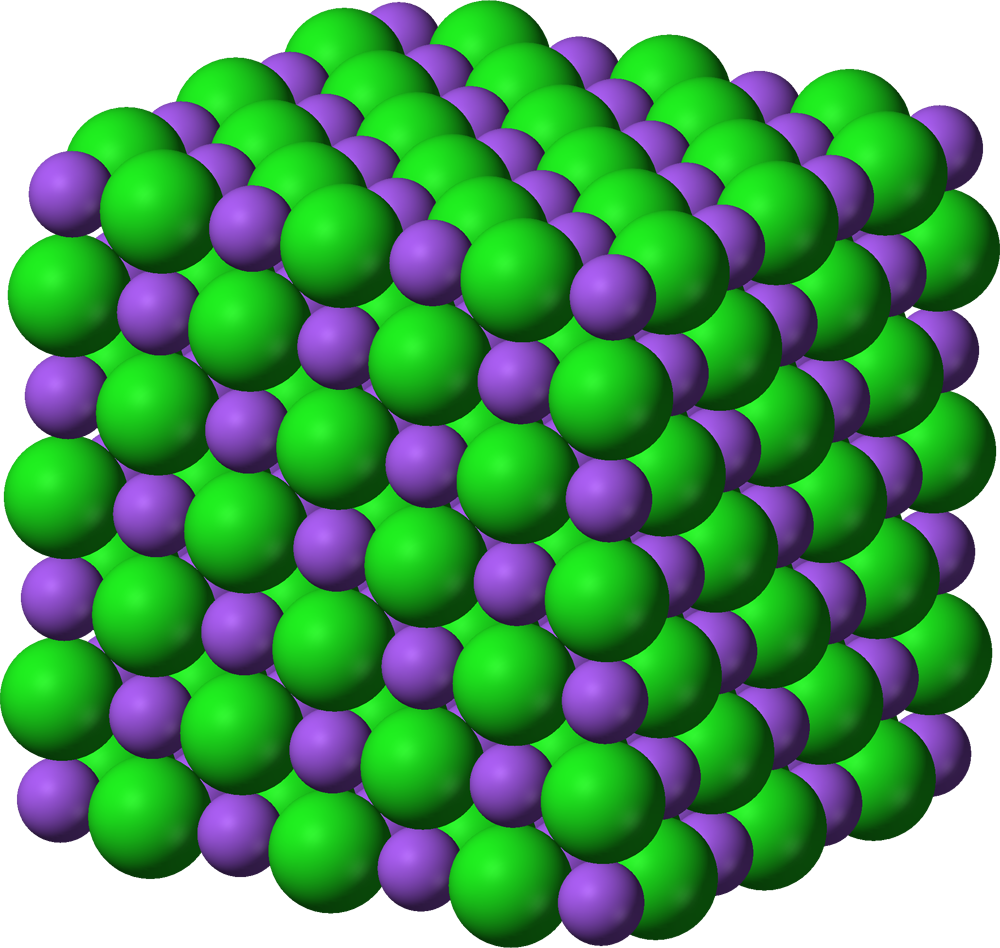
\includegraphics[width=4cm]{Sodium-chloride-3D-ionic.png}
\end{center}
includes the translations of space that move each green chlorine atom and purple natrium atom to its neighbor, up, down, left, right, forward or back, and mirror reflections around the coordinate planes through the origin, where we put the origin in the middle of any one of these atoms, and also the transformations given by permuting the order of the variables \(x,y,z\) of each coordinate axis.
\end{example}
\begin{example}
Every \(2 \times 2\) matrix 
\[
A=
\begin{pmatrix}
a & b \\
c & d
\end{pmatrix}
\]
(with entries from any chosen field) determines a \emph{linear transformation}\define{transformation!linear}\define{linear transformation}:
\[
\begin{pmatrix}
x \\
y
\end{pmatrix}
\mapsto
A
\begin{pmatrix}
x \\
y
\end{pmatrix}
=
\begin{pmatrix}
a & b \\
c & d
\end{pmatrix}
\begin{pmatrix}
x \\
y
\end{pmatrix}
=
\begin{pmatrix}
ax + by \\
cx + dy
\end{pmatrix}
\]
of the plane.
Similarly, a square matrix \(A\), say \(n \times n\), determines a linear transformation of \(n\)-dimensional Euclidean space.
A linear transformation is a bijection just when the associated matrix \(A\) is invertible, i.e. just when \(A\) has nonzero determinant.\SubIndex{determinant}
The invertible \(n \times n\) matrices form a transformation group \(G\), of linear transformations of \(n\)-dimensional Euclidean space.
\end{example}



\section{Permutations}
A transformation which is a bijection is also called a \emph{permutation}, especially when it transforms a finite set.
\begin{example}
Take \(X\) to be the set of numbers \(\set{1,2,3,4}\).
The \emph{symmetric group}\define{symmetric group} on 4 letters is the group \(G\) of all permutations of \(X\).
The terminology ``on 4 letters'' reminds us that we could just as well have taken \(X=\set{a,b,c,d}\) to consist of any 4 distinct elements, and then we would get essentially the same story, just relabelling.
It is convenient notation to write a permutation of finite sets as, for example,
\[
\begin{pmatrix}
1 & 2 & 3 & 4 \\
2 & 3 & 1 & 4
\end{pmatrix}
\]
to mean the map \(f\) so that \(f(1)=2\), \(f(2)=3\), \(f(3)=1\) and \(f(4)=4\), i.e. reading down from the top row as the input to \(f\) to the entry underneath as the output of \(f\).
It is often understood that the first row is just \(1234\) or some such, so we can just write down the second row: \(2314\), to display the permutation.
\end{example}

\begin{problem}{groups:compose.permutation}
What is are the permutations \(g \circ f\) and \(f \circ g\) where \(g\) is \(2314\) and \(f\) is \(3124\)?
\end{problem}

\begin{problem}{groups:tetrahedron}
A \emph{regular tetrahedron}\define{tetrahedron} is a pyramid with triangular base, all of whose sides are equilateral triangles.
Prove that the symmetry group of the regular tetrahedron is the symmetric group on 4 letters.
\end{problem}
\begin{answer}{groups:tetrahedron}
We can simply permutate the vertices in any way at all by symmetries, as we can rotate any one vertex to any other, and then fixing that vertex, the symmetries of the opposite faceare arbitrary symmetries of an equilateral triangle, so carry out any permutation of its vertices.
\end{answer}

Another notation for permutations: the \emph{cycle}\define{cycle} \((1 3 4 2)\) means the permutation that takes \(1\) to \(3\), \(3\) to \(4\), \(4\) to \(2\) and \(2\) to \(1\), reading from left to right.
More generally, the cycle \((a_1 a_2 \dots a_k)\) is the permutation taking \(a_1\) to \(a_2\), \(a_2\) to \(a_3\), and so on, and taking \(a_k\) to \(a_1\).
So \((2 3 1 4)\) takes \(3\) to \(1\).
By definition, if we have a number \(x\) which is not among these various \(a_1, a_2, \dots, a_k\), then the cycle \((a_1 a_2 \dots a_k)\) fixes the number \(x\):
\((2 3 5 4)\) takes \(1\) to \(1\).
Two cycles \((a_1 a_2 \dots a_k)\) and \((b_1 b_2 \dots b_{\ell})\) are \emph{disjoint}\define{cycle!disjoint} if none of the \(a_i\) occur among the \(b_j\) and vice versa.
So 
\[
(1 4 5 2) \text{ is disjoint from } (3 6),
\]
but
\[
(1 3 5 2) \text{ is not disjoint from } (3 6)
\]
since they both have \(3\) in them.
We can write the identity permutation as \(()\).
Note that any cycle of length 1 is also the identity transformation: \((2)=(1)=()\), since \((2)\) takes \(2\) to \(2\), and fixes everything else.
If two permutations \(f\) and \(g\) can be expressed as disjoint cycles, then \(fg=gf\), since each fixes all of the letters moved by the other.

\begin{problem}{permutations:disjointify}
Write \((123)(234)(543)\) as (a) a permutation in our first notation and (b) as  a product of disjoint cycles.
\end{problem}
\begin{answer}{permutations:disjointify}
Apply each cycle in succession to \(1\): \((543)1=1\), \((234)1=1\), \((123)1=2\). So \((123)(234)(543)1=2\).
Similarly apply them to \(2\): \((543)2=2\), \((234)2=3\), \((123)3=1\). So \((123)(234)(543)2=1\).
Continue in this way to find (a) \((123)(234)(543)=21543\).
Clearly this takes \(1 \to 2 \to 1\) and \(3 \to 5 \to 3\) and \(4 \to 4\), so (b) as a product of disjoint cycles
\((123)(234)(543)=(12)(35)\).
\end{answer}

Sage knows how to multiply cycles:
\begin{sageblock}
G = SymmetricGroup(5)
sigma = G("(1,3) (2,5,4)")
rho = G([(2,4), (1,5)])
rho^(-1) * sigma * rho
\end{sageblock}
prints \(\sage{rho^(-1) * sigma * rho}\).

\begin{theorem}
Every permutation of the elements of a finite set is expressed as a product of disjoint cycles, uniquely except for the order in which we write down the cycles, which can be arbitrary.
\end{theorem}
\begin{proof}
Suppose our finite set is \(1,2,\dots,n\); write these down in order in a list.
Pick a number and see what the permutation takes it to, and what it takes that number to, and so on, until eventually you return to the number you started at: a cycle.
Cross out all of those numbers from the list, and start again.
\end{proof}

For example, in cycle notation
\[
\begin{pmatrix}
1 & 2 & 3 & 4 \\
2 & 3 & 1 & 4
\end{pmatrix}
=(1 2 3)
\]
and
\[
\begin{pmatrix}
1 & 2 & 3 & 4 & 5 \\
3 & 4 & 1 & 5 & 2 
\end{pmatrix}
=(1 3)(2 4 5).
\]
\begin{problem}{permutations:cycle.product}
What is the product of cycles \((1234)(1423)(324)\) as a product of disjoint cycles?
Explain how you find your answer.
\end{problem}
\begin{answer}{permutations:cycle.product}
\((234)\): 
\begin{align*}
1 &\to 4 \to 1, \\
2 &\to 4 \to 2 \to 3, \\
3 &\to 2 \to 3 \to 4, \\
4 &\to 3 \to 1 \to 2.
\end{align*}
\end{answer}
\begin{problem}{permutations:cube}
Let \(G\) be the collection of all rotations of a cube.
How many rotations lie in \(G\)?
How does each decompose into a product of disjoint cycles acting on the faces of the cube?
\end{problem}
\begin{answer}{permutations:cube}
Indicate cycle lengths in a permutation by drawing boxes, a row of them to indicate a cycle of that length, arranged successively shorter: the \emph{Young diagram}\define{Young diagram} of a permutation.
For example, 
\[
\yng(4,3^2,2)
\]
indicates a permutation which has cycles of lengths \(4,3,3,2\).
The group \(G\) of rotations of a cube moves any vertex to any other (8 in all), and rotates a vertex around taking any edge at that vertex to any other (3 in all), but once we fix a vertex and edge, we fix everything, so the group has exactly \(8\cdot 3=24\) elements.
Every rotation is a rotation around an axis, through the centre of the cube.
It is determined completely by how it acts on the centres of the faces, as they contain a basis of vectors.
The identity \(1\) fixes every face, so has \(6\) cycles (all of length 1) as permutation of the faces.
A rotation of angle \(\pi\) around an axis through the center of a face fixes two faces and permutes two others, so a pair of disjoint cycles of length 2; there are 3 such, as there are three choices of axis.
A rotation of angle \(\pi\) around an axis through the center of an edge permutes three pairs of faces, so a triple of disjoint cycles of length 2; there are 6 such rotations.
An element of order 3 is a rotation around an axis through two opposite corners: it is a cycle of order 3 on the three faces touching one corner, and also of order 3 on the opposite three faces touching the opposite corner.
There are 4 choices of a pair of opposite corners, and then 2 directions of rotation, so 8 such rotations.
An element of order 4 is a rotation by angle \(\pi/2\), so around some axis through two opposite faces, giving one cycle of length 4; there are 3 choices of axis, but we can point the axis in either direction, so 6 such rotations.
We can sum the various permutations of the faces of cube arising from rotations as:
\[
\yng(1^6)+3\yng(2^2,1^2)+6\yng(2^3)+8\yng(3^2)+6\yng(4,1,1)
\]
\end{answer}
\begin{problem}{groups:count.perms}
Prove that any set with \(n\) elements has \(n!\) permutations, in several ways: by counting 
\begin{enumerate}
\item how many places to move \(1\) to, and then how many places there are left to move \(2\) to, and so on,
\item the number of places to stick object \(n\) in between the elements of any given permutation \(a_1 a_2 \dots a_{n-1}\) of the numbers \(1,2,\dots,n-1\), say as \(n a_1 a_2 \dots a_{n-1}\) or \(a_1 n a_2 \dots a_{n-1}\) or \(a_1 a_2 n \dots a_{n-1}\) and so on, for example: given the permutation \(312\) of the numbers \(123\), we can put \(4\) in there as
\[
4312, 3412, 3142, \text{ or } 3124.
\]
\item the number of ways to put at the end of a given permutation \(a_1 a_2 \dots a_{n-1}\) some number \(b\) from among 
\[
b=\frac{1}{2}, 1+\frac{1}{2}, \dots, n-\frac{1}{2},
\]
for example into the permutation \(312\) we stick
\[
312\frac{1}{2}, \quad \text{ or }
312\frac{3}{2}, \quad \text{ or }
312\frac{5}{2}, \quad \text{ or }
312\frac{7}{2}
\]
and then replace the numbers in the list by integers from \(1,2,\dots,n\), but in the same order:
\[
4231, 4132, 4123, \text{ or } 3124.
\]
\item
the possible disjoint cycles.
\end{enumerate}
\end{problem}
\begin{problem}{groups:symmetric.conjugacy.1}
Suppose that \(g\) is a permutation written as a product of disjoint cycles, say \(g=(1487)(235)\) as a permutation of 8 letters.
Take any permutation \(h\) of 8 letters.
Prove that 
\[
hgh^{-1}=(h(1)h(4)h(8)h(7))(h(2)h(3)h(5)).
\]
\end{problem}
\begin{answer}{groups:symmetric.conjugacy.1}
In general, if 
\[
g=\dots (a_1 a_2 \dots a_k) \dots
\]
where the \(\dots\) indicate other cycles, in a product of disjoint cycles, then \(hgh^{-1}\), when applied to \(h(a_i)\) gives
\begin{align*}
(hgh^{-1})(h(a_1))
&=
hgh^{-1}h(a_1),
\\
&=
hg(h^{-1}h)(a_1),
\\
&=
hg(a_1),
\\
&=
h(a_{2}),
\end{align*}
and so on: \(hgh^{-1}\) takes \(h(a_i)\) to \(h(a_{i+1})\) and takes \(h(a_n)\) to \(h(a_1)\).
If \(g\) is a product of cycles, the same thing works applied one at a time.
\end{answer}
\begin{problem}{groups:symmetric.conjugacy}
Prove that there is an element \(g\) of the symmetric group on 7 letters so that \((147)(23)\) and \((235)(14)\) are conjugate, i.e. \((235)(14)=g(147)(23)g^{-1}\).
More generally, prove that two elements of the symmetric group on \(n\) letters are conjugate just when, when we write them as products of disjoint cycles, the numbers of cycles of each length are the same. 
\end{problem}
\begin{answer}{groups:symmetric.conjugacy}
Start with just one cycle, say \((a_1a_2\dots a_k)\) and one cycle \((b_1b_2\dots b_k\).
Then let \(ga_1\defeq b_1\), \dots, \(ga_k\defeq b_k\), and let \(gx\defeq x\) for \(x\) not among \(a_1,\dots,a_k\).
Let's check that \((b_1\dots b_k)=g(a_1 \dots a_k)g^{-1}\).
The left hand side acts on \(b_1\) by moving it to \(b_2\), and so on.
The right hand side takes \(b_1\), applies \(g^{-1}\) to it, so gives \(a_1\), then moves \(a_1\) to \(a_2\), and then applies \(g\) to that, giving \(b_2\), and so on.
Now for two disjoint cycles, say 
\[
g_1 = (a_1 a_2 \dots a_k)(\alpha_1 \alpha_2 \dots \alpha_{\ell})
\]
and
\[
g_2 = (b_1 b_2 \dots b_k)(\beta_1 \beta_2 \dots \beta_{\ell}),
\]
let \(ga_i \defeq b_1\) and \(g\alpha_i\defeq \beta_i\) and \(gx=x\) for any other \(x\).
Again check that \(g_2=gg_1g^{-1}\).
Proceed by induction.
\end{answer}
A \emph{transposition}\define{transposition} is a 2-element cycle.
Every cycle has an obvious decomposition as a product of transpositions: \((1234)=(12)(23)(34)\), and so on: 
\begin{problem}{permutations:cycle.as.transpositions}
Prove that \((123\dots n)=(12)(23)(34)\dots(n-1 \ n)\).
\end{problem}
Hence we can break any permutation into an obvious product of transpositions.
\begin{problem}{permutations:transposition.product}
Write the permutation \((17)\) as a product of transpositions of neighboring integers.
\end{problem}
\begin{answer}{permutations:transposition.product}
\((12)(23)(34)(45)(56)(67)(56)(45)(34)(23)(12)\)
\end{answer}
Given a polynomial \(b(t)\) in variables \(t_1,t_2,\dots,t_n\), and a permutation \(p\) of \(n\) letters, we define \(pb(t)\) by the equation
\[
pb(t_1,\dots,t_n)=b(t_{q(1)},\dots,t_{q(n)}),
\]
where \(q\) is the inverse permutation to \(p\).
\begin{example}
If \(p=2314\) then \(q=3124\). If
\[
b(t_1,t_2,t_3,t_4)=t_1^6+8t_2t_4+t_3^9,
\]
then
\[
pb(t_1,t_2,t_1,t_4)=t_3^6+8t_1t_4+t_2^9.
\]
\end{example}
\begin{problem}{groups:compose.poly}
If \(p,r\) are permutations on \(n\) letters prove that \(r(pb)=(rp)b\) for any polynomial \(b\) in \(n\) variables.
\end{problem}
\begin{answer}{groups:compose.poly}
Let \(q\defeq p^{-1}\) and \(s\defeq r^{-1}\), so
\begin{align*}
(r(pb))(t_1,\dots,t_n)
&=
pb(t_{s(1)},\dots,t_{s(n)}),
\\
&=
b(t_{q(s(1))},\dots,t_{q(s(n))}),
\\
&=
b(t_{q \circ s(1))},\dots,t_{q \circ s(n))}),
\\
&=
(q \circ s)^{-1}b(t_1,\dots,t_n),
\\
&=
(s^{-1} \circ q^{-1})b(t_1,\dots,t_n),
\\
&=
(rp)b(t_1,\dots,t_n).
\end{align*}
\end{answer}
The \emph{sign}\define{sign!permutation}\define{permutation!sign} of a permutation \(p\), denoted \((-1)^p\), is \((-1)^t\) where \(t\) is the number of transpositions in some expression of \(p\) as a product of transpositions of neighboring integers.
\begin{lemma}\label{lemma:sign.of.permutation}
The map taking a permutation \(p\) to its sign, denoted \((-1)^p\), is well defined and satisfies \((-1)^{pq}=(-1)^p(-1)^q\) for any two permutations \(p,q\) of the same number of letters.
Moreover \((-1)^p=(-1)^t\) if \(p\) can be written as as product of \(t\) transpositions.
\end{lemma}
\begin{proof}
Consider the polynomial
\[
b(t_1,\dots,t_n)=(t_1-t_2)(t_1-t_3)\dots(t_{n-1}-t_n)=\prod_{i<j}(t_i - t_j).
\]
Then \(pb(t)\) has various \(t_i-t_j\) factors multiplied together, with \(i \ne j\), in every possible pairing of \(i,j\) or \(j,i\).
So \(pb(t)=\pm b(t)\).
Write this \(\pm\) as \((-1)^p\).

Suppose that \(p\) is the transposition \((i \ \ i+1)\).
Then \(p\) changes \(t_i-t_{i+1}\) into \(t_{i+1}-t_i=-(t_i-t_{i+1})\), one sign change.
Otherwise, \(p\) leaves everything in \(b(t)\) as it is except swapping \(t_i-t_j\) and \(t_{i+1}-t_j\) for \(j \ge i+2\), and swapping \(t_j-t_i\) and \(t_j-t_{i+1}\) for \(j \le i-1\).
So finally, only one sign change: \(pb(t)=-b(t)\), so \((-1)^p=-1\).

If \(p,q\) are any two permutations of \(n\) letters, then \((-1)^p(-1)^qb=p(qb)=(pq)b=(-1)^{pq}b\).
Therefore, for any \(i\) and \(j\), if we write
\[
(i \ \ i+1)=(i+1 \ \ j)(i \ \ j)(i+1 \ \ j),
\]
then \((-1)^{(ij)}=(-1)^{(i \ \ i+1)}=-1\).
\end{proof}
\begin{problem}{permutations:transposition}
Prove that the sign of any transposition is \(-1\) by writing it as a product number of transpositions of neighboring integers.
\end{problem}
\begin{answer}{permutations:transposition}
We can transpose \(i\) and \(i+1\) as \((i \ \ i+1)\).
We can transpose \(i\) and \(i+2\), as a product \((i \ \ i+1)(i+1 \ \ i+2)(i \ \ i+1)\).
Similarly, we can write any transposition as a product of an odd number of transpositions of neighboring integers: if \(i<j\),
\[
(i \ \ j)=(i \ \ i+1)(i+1 \ \ i+2)\dots(j-2 \ \ j-1)(j-1 \ \ j)\dots(i+1 \ \ i+2)(i \ \ i+1).
\]
\end{answer}
\begin{problem}{permutions:rationals}
Prove that, over any field, any symmetric rational function (i.e. permutation invariant) has an expression \(b(e_1,\dots,e_n)/c(e_1,\dots,e_n)\) as a ratio of polynomials with no common nonconstant factor, expressed in the elementary symmetric polynomials, unique up to rescaling numerator and denominator by the same nonzero constant.
\end{problem}
\begin{answer}{permutions:rationals}
If there were two such, cross multiply and apply unique factorisation of polynomials (theorem~\vref{theorem:ufd}).
Two see that there is one such, write out the function as \(p(x_1,\dots,x_n)/q(x_1,\dots,x_n)\).
Apply a permutation of the variables, and the solution of problem~\vref{problem:factoring:rationals}, to see that each permutation alters the numerator by a nonzero constant multiple, and the denominator by the same multiple.
Swapping two variables gives some multiple, and repeating that swap gives the same multiple squared, but returns to the original order of the variables.
So any swap either changes sign or leaves both numerator and denominator alone.
Multiple the numerator and denominator by the function \(\prod_{i<j}(t_i - t_j)\) to ensure that the don't change when we transpose, and so they don't change under any permutation.
Apply theorem~\vref{theorem:symmetric.polynomials.algebra}.
\end{answer}
\begin{problem}{permutations:det}
Starting from your favourite definition of determinant of a square matrix, prove that for any square matrix \(A\), say of size \(n \times n\), with coefficients in any field,
\[
\det A = \sum_p (-1)^p A_{1p(1)}A_{2p(2)} \dots A_{np(n)},
\]
where the sum is over all permutations \(p\) of \(1,2,\dots,n\).
\end{problem}
The group of even permutations of \(n\) letters is the \emph{alternating group}.
\begin{problem}{permutations:alt.4}
Write out the elements of the alternating group on \(4\) letters.
\end{problem}
\begin{problem}{permutations:alt}
Prove that the alternating group on \(n\) letters contains \(n!/2\) elements.
\end{problem}
\begin{problem}{permutations:15}
The 15-puzzle is a \(4 \times 4\) square containing with 15 slideable tiles (each a \(1 \times 1\) square), so one square is vacant (i.e. has no tile in it):
\begin{center}
\documentclass[tikz]{standalone}
\begin{document}
\begin{tikzpicture}[scale=.3]
\fill[gray!20] (0,0) rectangle (4,4);
\fill[white] (2,1) rectangle (3,2);
\draw[gray!50] (0,0) grid (4,4);
\node at (.5,3.5) {\tiny{7}};
\node at (1.5,3.5) {\tiny{5}};
\node at (2.5,3.5) {\tiny{2}};
\node at (3.5,3.5) {\tiny{11}};
\node at (.5,2.5) {\tiny{3}};
\node at (1.5,2.5) {\tiny{10}};
\node at (2.5,2.5) {\tiny{1}};
\node at (3.5,2.5) {\tiny{12}};
\node at (.5,1.5) {\tiny{13}};
\node at (1.5,1.5) {\tiny{9}};
%\node at (2.5,1.5) {\tiny{1}};
\node at (3.5,1.5) {\tiny{6}};
\node at (.5,.5) {\tiny{14}};
\node at (1.5,.5) {\tiny{4}};
\node at (2.5,.5) {\tiny{15}};
\node at (3.5,.5) {\tiny{8}};
\end{tikzpicture}
\end{document}
\end{center}
Each tile has a number on it, from 1 to 15.
We solve the puzzle by sliding the squares around until they lie in order by number, with the vacant square last:
\begin{center}
\documentclass[tikz]{standalone}
\begin{document}
\begin{tikzpicture}[scale=.3]
\fill[gray!20] (0,0) rectangle (4,4);
\fill[white] (3,0) rectangle (4,1);
\draw[gray!50] (0,0) grid (4,4);
\node at (.5,3.5) {\tiny{1}};
\node at (1.5,3.5) {\tiny{2}};
\node at (2.5,3.5) {\tiny{3}};
\node at (3.5,3.5) {\tiny{4}};
\node at (.5,2.5) {\tiny{5}};
\node at (1.5,2.5) {\tiny{6}};
\node at (2.5,2.5) {\tiny{7}};
\node at (3.5,2.5) {\tiny{8}};
\node at (.5,1.5) {\tiny{9}};
\node at (1.5,1.5) {\tiny{10}};
\node at (2.5,1.5) {\tiny{11}};
\node at (3.5,1.5) {\tiny{12}};
\node at (.5,.5) {\tiny{13}};
\node at (1.5,.5) {\tiny{14}};
\node at (2.5,.5) {\tiny{15}};
%\node at (3.5,.5) {\tiny{8}};
\end{tikzpicture}
\end{document}
\end{center}
Prove that if the 15-puzzle starts in this order:
\begin{center}
\documentclass[tikz]{standalone}
\begin{document}
\begin{tikzpicture}[scale=.3]
\fill[gray!20] (0,0) rectangle (4,4);
\fill[white] (3,0) rectangle (4,1);
\draw[gray!50] (0,0) grid (4,4);
\node at (.5,3.5) {\tiny{1}};
\node at (1.5,3.5) {\tiny{2}};
\node at (2.5,3.5) {\tiny{3}};
\node at (3.5,3.5) {\tiny{4}};
\node at (.5,2.5) {\tiny{5}};
\node at (1.5,2.5) {\tiny{6}};
\node at (2.5,2.5) {\tiny{7}};
\node at (3.5,2.5) {\tiny{8}};
\node at (.5,1.5) {\tiny{9}};
\node at (1.5,1.5) {\tiny{10}};
\node at (2.5,1.5) {\tiny{11}};
\node at (3.5,1.5) {\tiny{12}};
\node at (.5,.5) {\tiny{13}};
\node at (1.5,.5) {\tiny{15}};
\node at (2.5,.5) {\tiny{14}};
%\node at (3.5,.5) {\tiny{8}};
\end{tikzpicture}
\end{document}
\end{center}
it is not solvable.
Hint: associate to each permutation (of tiles and vacant square) a number \(x=0\) or \(1\), depending on whether the permutation of the order of the tiles (ignoring the vacant spot) is even or odd, and a number \(y=0\) or \(1\) given by the row of the vacant spot, modulo \(2\).
Let \(z=x+y\) modulo 2.
\end{problem}
\begin{answer}{permutations:15}
If we make a move by sliding a tile left or right, we don't change \(x\) or \(y\), so \(z\) is the same.
If we make a move by sliding a tile up or down, we change \(y\) and also carry out a cycle in the order of the tiles.
If that tile is in the first column, we are making a cycle of length 4:
\begin{center}
\documentclass[tikz]{standalone}
\begin{document}
\begin{tikzpicture}[scale=.3]
\fill[gray!20] (0,0) rectangle (4,4);
\fill[white] (0,1) rectangle (1,2);
\draw[gray!50] (0,0) grid (4,4);
\node at (.5,3.5) {\tiny{1}};
\node at (1.5,3.5) {\tiny{2}};
\node at (2.5,3.5) {\tiny{3}};
\node at (3.5,3.5) {\tiny{4}};
\node at (.5,2.5) {\tiny{5}};
\node at (1.5,2.5) {\tiny{6}};
\node at (2.5,2.5) {\tiny{7}};
\node at (3.5,2.5) {\tiny{8}};
%\node at (.5,1.5) {\tiny{9}};
\node at (1.5,1.5) {\tiny{10}};
\node at (2.5,1.5) {\tiny{11}};
\node at (3.5,1.5) {\tiny{12}};
\node at (.5,.5) {\tiny{13}};
\node at (1.5,.5) {\tiny{15}};
\node at (2.5,.5) {\tiny{14}};
\node at (3.5,.5) {\tiny{8}};
\draw[shorten >=1pt,shorten <=1pt,blue!75,-stealth] (.5,.5) -- (.5,1.5);
\end{tikzpicture}
\end{document}
\end{center}
and the same for any other column, since we have one less square above and one more below.
So the value of \(x\) always changes.
So \(z\) stays the same.
The initial picture:
\begin{center}
\documentclass[tikz]{standalone}
\begin{document}
\begin{tikzpicture}[scale=.3]
\fill[gray!20] (0,0) rectangle (4,4);
\fill[white] (3,0) rectangle (4,1);
\draw[gray!50] (0,0) grid (4,4);
\node at (.5,3.5) {\tiny{1}};
\node at (1.5,3.5) {\tiny{2}};
\node at (2.5,3.5) {\tiny{3}};
\node at (3.5,3.5) {\tiny{4}};
\node at (.5,2.5) {\tiny{5}};
\node at (1.5,2.5) {\tiny{6}};
\node at (2.5,2.5) {\tiny{7}};
\node at (3.5,2.5) {\tiny{8}};
\node at (.5,1.5) {\tiny{9}};
\node at (1.5,1.5) {\tiny{10}};
\node at (2.5,1.5) {\tiny{11}};
\node at (3.5,1.5) {\tiny{12}};
\node at (.5,.5) {\tiny{13}};
\node at (1.5,.5) {\tiny{15}};
\node at (2.5,.5) {\tiny{14}};
%\node at (3.5,.5) {\tiny{8}};
\end{tikzpicture}
\end{document}
\end{center}
differs from the final one:
\begin{center}
\documentclass[tikz]{standalone}
\begin{document}
\begin{tikzpicture}[scale=.3]
\fill[gray!20] (0,0) rectangle (4,4);
\fill[white] (3,0) rectangle (4,1);
\draw[gray!50] (0,0) grid (4,4);
\node at (.5,3.5) {\tiny{1}};
\node at (1.5,3.5) {\tiny{2}};
\node at (2.5,3.5) {\tiny{3}};
\node at (3.5,3.5) {\tiny{4}};
\node at (.5,2.5) {\tiny{5}};
\node at (1.5,2.5) {\tiny{6}};
\node at (2.5,2.5) {\tiny{7}};
\node at (3.5,2.5) {\tiny{8}};
\node at (.5,1.5) {\tiny{9}};
\node at (1.5,1.5) {\tiny{10}};
\node at (2.5,1.5) {\tiny{11}};
\node at (3.5,1.5) {\tiny{12}};
\node at (.5,.5) {\tiny{13}};
\node at (1.5,.5) {\tiny{14}};
\node at (2.5,.5) {\tiny{15}};
%\node at (3.5,.5) {\tiny{8}};
\end{tikzpicture}
\end{document}
\end{center}
by a single transposition, with no row swap, so different value of \(z\).
\end{answer}

\section{Sage}
Sage knows all of the permutations of small symmetric groups, and will print them out for you in cycle notation:
\begin{sageblock}
H = DihedralGroup(6)
H.list()
\end{sageblock}
yields
\[
\begin{array}{lll}
               , & (1,6)(2,5)(3,4), & (1,2,3,4,5,6), \\ 
     (1,5)(2,4), & (2,6)(3,5),      & (1,3,5)(2,4,6), \\ 
(1,4)(2,3)(5,6), & (1,6,5,4,3,2),   & (1,4)(2,5)(3,6), \\ 
(1,2)(3,6)(4,5), & (1,5,3)(2,6,4),  & (1,3)(4,6)
\end{array}
\]
where the identity element is the blank space at the start.

\chapter{Young diagrams}

\section{Introduction}
Every polynomial \(f(x,y)\) of two variables is a sum
\[
f(x,y) = f_+(x,y) + f_-(x,y),
\]
of a symmetric polynomial and an antisymmetric polynomial, where we let
\begin{align*}
f_+(x,y)&\defeq \frac{1}{2}\pr{f(x,y)+f(y,x)},\\
f_-(x,y)&\defeq \frac{1}{2}\pr{f(x,y)-f(y,x)},
\end{align*}
be the symmetric and antisymmetric parts.
We want to generalize to many variables.

\section{Definition}
A \emph{Young diagram}:\define{Young!diagram}\define{diagram!Young}
\[
\yng(4^2,3,2^3,1)
\]
is a collection of boxes, arranged in rows and columns, all rows aligned vertically along their left edges, so that each row is as long or shorter than any above it.
Write down the number of boxes in each row in a sequence: \([4,4,3,2,2,2,2,1]\), called the \emph{partition}\define{partition} of the Young diagram, and denoted \(\lambda\).
So we let \(\lambda_1\) be the number of boxes in row 1, \(\lambda_2\) the number in row 2, and so on, say up to \(r\) rows, and write \(\lambda\defeq [\lambda_1,\lambda_2,\dots,\lambda_r]\).
If you know the partition, you can draw the Young diagram, and vice versa, so we could sometimes confuse the two, and write that they are equal:
\[
[4,4,3,2,2,2,1]=\yng(4^2,3,2^3,1).
\]

\begin{problem}{young:all}
Draw all Young diagrams with at most 5 boxes.
\end{problem}
\begin{answer}{young:all}
{
\arraycolsep=1.4pt\def\arraystretch{2.2}
\setlength{\arraycolsep}{10pt}
\[
\begin{array}{ccccccccccc}
\yng(1)\\
\yng(2)&\yng(1,1)\\
\yng(3)&\yng(2,1)&\yng(1,1,1)\\
\yng(4)&\yng(3,1)&\yng(2,2)&\yng(2,1,1)&\yng(1,1,1,1)\\
\yng(5)&\yng(4,1)&\yng(3,2)&\yng(3,1,1)&\yng(2,2,1)&\yng(2,1,1,1)&\yng(1,1,1,1,1)
\end{array}
\]
}
\end{answer}

Take a Young diagram \(\lambda\) with entries \(1,2,\dots,n\) put in order, and a permutation \(p\).
Write \(\lambda^p\) to mean the application of \(p\) to all entries in \(\lambda\).
\begin{example}
\[
\lambda=\young(1234,567,8,9),
\]
and \(p=52938971\) gives
\[
\lambda^p=\young(5293,847,6,1)
\]
\end{example}
\begin{lemma}\label{lemma:moves.two}
Take a Young diagram \(\lambda\), with entries \(1,2,\dots,n\) put in order, 
\[
\lambda=\young(1234,567,8,9),
\]
Each permutation \(p\) either 
\begin{enumerate}
\item
moves two entries that lie in the same row into the same column or
\item
is uniquely expressed as product \(p=rc\) of a permutation \(r\) preserving the rows, and a permutation \(c\) preserving the columns.
\end{enumerate}
\end{lemma}
\begin{example}
\[
\lambda=\young(1234,567,8,9),
\]
and \(p=52938971\) gives
\[
\lambda^p=\young(!\emphYoungBox5!\otherEmphYoungBox2!\regYoungBox93,8!\otherEmphYoungBox4!\regYoungBox7,!\emphYoungBox6,!\regYoungBox1)
\]
\end{example}
\begin{proof}
If \(p\) is expressed as such a permutation, suppose it arises two different ways: \(p=r_0c_0=r_1c_1\).
Then \(r_1^{-1}r_0=c_1c_0^{-1}\).
The left hand side preserves the rows, and the right hand the columns, so every element is taken to the same row and column, i.e. stays where it is: \(r_1^{-1}r_0=c_1c_0^{-1}=1\), and so \(r_0=r_1\) and \(c_0=c_1\).

On the other hand, suppose that any two entries in the same row end up, after some permutation \(p\), in different columns.
We want to prove that \(p\) is product of a row-preserving permutation and a column-preserving one.
Apply \(p\), and look where the entries from the first row ended up, all in different columns.
Take one transposition for each column, to get those entries back into the first row, perhaps in some strange order, and let \(q\) be the product of those transpositions.
\begin{example}
If
\[
\lambda^p=\young(!\emphYoungBox5!\regYoungBox293,847,6,!\emphYoungBox1)
\]
and we want to swap \(5\) and \(1\), these are in positions \(1\) and \(9\), so we take \(q=(19)\):
\[
\lambda^{pq}=\young(!\emphYoungBox1!\regYoungBox293,847,6,!\emphYoungBox5)
\]
\end{example}
It suffices to prove that  \(pq\) is such a product \(rc\).
So we can rename \(pq\) to call it \(p\), or in other words, we can assume that \(p\) preserves the first row.
Look where the entries from the second row ended up, all in different columns.
Take one transposition for each column, to get those entries back into the second row, perhaps in some strange order, say by some \(q\), and so on.
\end{proof}


Alphabetically order partitions: so \(\lambda=[6,6,5,\dots]\) is \emph{bigger} than \(\mu=[6,6,4,\dots\), because \(5 > 4\); if the first entries are equal, look at the second, and so on, until you hit a tie breaker.
Order Young diagrams by order of partition, i.e. by number of boxes in the first row, and if there is a tie, pass to the second row, and so on.

\begin{lemma}\label{lemma:scramble}
If \(\lambda,\mu\) are Young diagrams with \(n\) boxes, and \(\lambda > \mu\) then, no matter how we place the numbers \(1,2,\dots,n\) into the boxes of \(\lambda\), and into the boxes of \(\mu\), there are always two integers which lie in the same row in \(\lambda\) and also lie in the same column in \(\mu\).
\end{lemma}
\begin{proof}
For big enough \(k\), the first \(k\) rows of \(\lambda\) have more entries than the first \(k\) of rows of \(\mu\).
As we go down a Young diagram, rows can get shorter but not longer.
So the first \(k\) rows of \(\lambda\) have more entries than any \(k\) of rows of \(\mu\).
Pick out the entries from those \(k\) rows of \(\lambda\), and paste them into the boxes of \(\mu\), in any order at all.
We cannot distribute those entries over only \(k\) rows of \(\mu\); we need to use at least one more row.
Suppose we distribute those entries into at most \(k\) in each column.
Push them up into the uppermost boxes of those columns: they fit into \(k\) rows, impossible.
So there are some \(k+1\) in the same column of \(\mu\).
Some two of these must arise from the same row of \(\lambda\).
\end{proof}


\section{Young diagrams act on polynomials}
Given a Young diagram, we think of it as if it had a variable in each box, and it will ``act on'' any polynomial \(f\) of these variables.
So
\[
\young(abcd,efgh,ij,k)
\]
is a Young diagram acting on polynomials
\[
f(a,b,c,d,e,f,g,h,i,j,k).
\] 

\begin{example}
The diagram \([3]=\yng(3)\) will act on polynomial of 3 variables, i.e. \(f(a,b,c)\), by symmetrically averaging:
\[
\yng(3) f(a,b,c)=\frac{f(a,b,c)+f(a,c,b)+f(b,a,c)+f(b,c,a)+f(c,a,b)+f(c,b,a)}{6}.
\]
\end{example}

\begin{example}
The diagram \([1,1,1]=\yng(1^3)\) will antisymmetrize in 3 variables, 
\[
[1,1,1]f(a,b,c)=\frac{f(a,b,c)-f(a,c,b)-f(b,a,c)+f(b,c,a)+f(c,a,b)-f(c,b,a)}{6}.
\]
\end{example}
Soon we will explain how Young diagrams act in general. 

\section{Permutations act on polynomials}
Given a polynomial \(f(t)\) in variables \(t_1,t_2,\dots,t_n\), and a permutation \(p\) of \(n\) letters, we define \(pf(t)\) by the equation
\[
pf(t_1,\dots,t_n)=f(t_{q(1)},\dots,t_{q(n)}),
\]
where \(q\) is the inverse permutation to \(p\).
\begin{example}
If \(p=2314\) then \(q=3124\) so if we take
\[
f(t_1,t_2,t_3,t_4)\defeq t_1^6+8t_2t_4+t_3^9,
\]
then
\[
pf(t_1,t_2,t_1,t_4)=t_3^6+8t_1t_4+t_2^9.
\]
\end{example}
\begin{problem}{young:permute.poly}
If \(p=(123)(45)\) and \(f(t_1,t_2,t_3,t_4,t_5)=t_1^2 + t_2t_3+t_1t_4^5\), what is \(pf\)?
\end{problem}
\begin{answer}{young:permute.poly}
\(p^{-1}=(132)(45)\), so \(pf(t_1,t_2,t_3,t_4,t_5)=t_3^2 + t_1t_2+t_3t_5^5\).
\end{answer}
To save space, we write \(p\) to mean the operation taking \(f\) to \(pf\) too.
So when we write \((12)\), we could mean the cycle \((12)\), or the operation \((12)f(t_1,t_2)=f(t_2,t_1)\).
\begin{lemma}\label{lemma:permutations.independent}
The permutations of variables act as linearly independent operations on homogeneous polynomials of any fixed positive degree, with coefficients in any field.
\end{lemma}
\begin{proof}
Fix a degree \(k\ge 0\) and a number of variables \(n\).
If \(n=1\), the only permutation is the identity \(()\).
We want to prove that there is no nonzero linear combination, say \(a()\), which acts as zero.
But the action is \(()f=f\), so \(0=a()t^k=at^k=\) implies \(a=0\).

Suppose by induction that the result is proven for all integers less than \(n\).
Consider the action of some linear combination of permutations on polynomials in variables \(t_1,\dots,t_n\), say a linear combination 
\[
0 = \sum_p a_p p
\]
where the sum is over permutations, and the \(a_p\) are some coefficients from our field.
In other words,
\[
0 = \sum_p a_p pf
\]
for any homogeneous polynomial \(f(t_1,\dots,t_n)\) of degree \(k\).
Multiply \(f\) by a polynomial of any degree: the same equation
\[
0 = \sum_p a_p pf
\]
holds for all polynomials homogeneous of any degree at least \(k\).
Let \(f\) be a monomial
\[
f(t_1,\dots,t_n)=t_1^{b_1}\dots t_{n-1}^{b_{n-1}},
\]
with no \(t_n\) factors, and positive degrees \(b_1,b_2,\dots,b_{n-1}>0\) adding to at least \(k\).
For each permutation \(p\) of \(1,2,\dots,n\), consider the expression
\[
(pf)(t_1,\dots,t_{n-1},0).
\]
Clearly this vanishes just when \(t_n\) appears in \(pf\), i.e. just when \(p(n)\ne n\).
So
\[
0 = \sum_p a_p (pf)(t_1,\dots,t_{n-1},0)
\]
and every term drops out unless \(p(n)=n\), i.e. \(p\) is a permutation of \(1,2,\dots,n-1\).
Write \(\sum'\) for the sum of permutations of \(1,2,\dots,n-1\):
\[
0 = {\sum_p}' a_p (pf)(t_1,\dots,t_{n-1},0)
\]
The same holds for ratios of such monomials, and so for any monomial in \(t_1,\dots,t_{n-1}\), and therefore for any linear combination of monomials, i.e. for any polynomial \(f\) of \(n-1\) variables.
By induction on \(n\), \(a_p=0\) for each coefficient \(a_p\) in front of any permutation \(p\) fixing \(n\).

Take our relation \(0 = \sum a_p p\).
Pick any permutation \(q\).
Multiply the relation by \(q^{-1}\) to arrange that \(q=()\).
But then \(q\) fixes \(n\) so \(a_q=0\).
So all \(a_p\) vanish.
\end{proof}


\section{Sets give sums of permutations}
Take any set \(A\) of numbers from \(1,\dots,n\), and any polynomial \(f\) of \(n\) variables. Let
\[
A_+f\defeq\sum_p pf,
\]
where the sum is over permutations \(p\) of \(1,\dots,n\) which fix every number not in \(A\).
Similarly,
\[
A_-f\defeq\sum_p (-1)^p pf,
\]
with the sum over the same permutations.
\begin{example}
From among the numbers \(1,2,3,4\), take \(A\defeq\set{2,3}\).
The permutations of \(1,2,3,4\) fixing every number outside \(A\) are \(p=(23)\) or \(p=()\), giving
\[
A_+ f(t_1,t_2,t_3,t_4) = f(t_1,t_2,t_3,t_4)+f(t_1,t_3,t_2,t_4),
\]
and
\[
A_- f(t_1,t_2,t_3,t_4) = f(t_1,t_2,t_3,t_4)-f(t_1,t_3,t_2,t_4),
\]
\end{example}
\begin{problem}{young:permute.poly}
If \(A=234\), as a subset of \(12345\), what is \(A_+\)? What is \(A_-\)?
\end{problem}
\begin{answer}{young:permute.poly}
The permutations of \(234\) are 
\[
(),(23),(24),(34),(234),(243), 
\]
and each appears along with its inverse here, so we can write the inverses as 
\[
(),(23),(24),(34),(243),(234).
\]
So
\begin{align*}
234_+ f(t_1,t_2,t_3,t_4,t_5)
&=
f(t_1,t_2,t_3,t_4,t_5)+f(t_1,t_3,t_2,t_4,t_5)+f(t_1,t_4,t_3,t_2,t_5)\\
&\qquad
+f(t_1,t_2,t_4,t_3,t_5)+f(t_1,t_4,t_2,t_3,t_5)+f(t_1,t_3,t_4,t_2,t_5)
\end{align*}
A transposition like \((23)\) has sign \(-1\), and more generally a cycle of even length has sign \(-1\), while a cycle of odd length has sign \(1\):
\begin{align*}
234_- f(t_1,t_2,t_3,t_4,t_5)
&=
f(t_1,t_2,t_3,t_4,t_5)-f(t_1,t_3,t_2,t_4,t_5)-f(t_1,t_4,t_3,t_2,t_5)\\
&\qquad
-f(t_1,t_2,t_4,t_3,t_5)+f(t_1,t_4,t_2,t_3,t_5)+f(t_1,t_3,t_4,t_2,t_5).
\end{align*}
\end{answer}
It is convenient to think about permutations as operations on polynomials, and add permutations by adding their operations on polynomials, so we write
\[
A_+=\sum_p p,
\]
to mean
\[
A_+f\defeq\sum_p pf,
\]
and so on.
\begin{example}
From among the numbers \(1,2,3,4\), again take \(A\defeq\set{2,3}\).
The permutations of \(1,2,3,4\) fixing every number outside \(A\) are \(p=(23)\) or \(p=()\), giving
\[
A_+ = () + (23),
\]
and
\[
A_- = () - (23).
\]
We write \(A\) as \(A=23\), and write this as
\[
23_+ = () + (23),
\]
and
\[
23_- = () - (23).
\]
Notice that if we multiply by \((23)\),
\begin{align*}
A_+ (23)
&=
23_+(23),
\\
&=
\big(()+(23)\big)(23),
\\
&=(23)+(23)^2,
\\
&=(23)+(),
\\
&=23_+,
\\
&=A_+.
\end{align*}
Similarly, \(A_-q=qA_-=(-1)^qA_-\).
\end{example}

\begin{lemma}
If \(p\) is a permutation fixing all numbers from \(1,\dots,n\) except in a set \(A\), then
\(A_+ p = p A_+\) and \(A_- p = (-1)^p A_-\).
\end{lemma}
\begin{proof}
In each case, we are just rewriting our permutations in a different order, as multiplying by \(p\) reorders the permutations in the sum.
But in the case of \(A_-\), we are also messing up the signs by the sign of \(p\) in every permutation.
\end{proof}

\begin{lemma}\label{lemma:two.in.common}
If \(A,B \subset \set{1,\dots,n}\) share two elements or more in common, then \(0=A_+ B_-=B_-A_+=A_-B_+=B_+A_-\).
\end{lemma}
\begin{proof}
Suppose for simplicity that \(1\) and \(2\) belong to both \(A\) and \(B\).
Then \(A_+B_-(12)=A_+(-1)B_-=(-1)A_+B_-\), so \(A_+B_-=0\), and similarly for the other cases.
\end{proof}

\section{How Young diagrams act}
Given a Young diagram \(\lambda\), 
\[
\lambda = \yng(3,3,2,1)
\]
say with \(n\) boxes, write the integers \(1,2,\dots,n\) into the boxes in order:
\[
\young(123,456,78,9).
\]
Let \(\lambda_+\) be the product of the \({}_+\) operators of each row.
In our example,
\begin{align*}
\lambda_+ 
&= 
123_+ 456_+ 78_+ 9_+,
\\
&=
\big(()+(12)+(13)+(23)+(123)+(132)\big)
\big(()+(45)+(46)+(56)+(456)+(465)\big)
\big(()+(78)\big)
\big(()\big),
\end{align*}
expands out to something very large.
Similarly, \(\lambda_-\) is the product of the \({}_-\) operators of the columns.
In our example,
\[
\lambda_-=1479_- 258_- 36_-,
\]
which expands out to something even larger.

\begin{problem}{young:lambda.p}
Writing \(\lambda^p_+\) to mean \((\lambda^p)_+\), prove that \(\lambda^p_+=p\lambda_+p^{-1}\) and \(\lambda^p_-=p\lambda_-p^{-1}\).
\end{problem}
\begin{answer}{young:lambda.p}
Let \(\mu\defeq\lambda^p\).
So \(\mu_+\) acts on polynomials by products of permutations of the rows of \(\mu\).
But if \(\lambda\) has a row 
\[
a_1 a_2 \dots a_k,
\]
then \(\mu\) has corresponding row 
\[
p(a_1) p(a_2) \dots p(a_k).
\]
In \(\lambda_+\), this row produces permutations which are products of cycles of the form 
\[
(a_{i_1} \ a_{i_2} \ \dots \ a_{i_{\ell}}).
\]
As in problem~\vref{problem:groups:symmetric.conjugacy.1}, in \(\mu_+\), each such cycle yields a cycle of the form 
\[
(p(a_{i_1}) \ p(a_{i_2}) \ \dots \ p(a_{i_{\ell}})).
\]
Similarly for columns instead of rows and \(\lambda_-\) instead of \(\lambda_+\).
\end{answer}

Each Young diagram \(\lambda\) acts on polynomials as the operation
\[
\lambda = \frac{\sum_p \lambda^p_+ \lambda^p_-}{N^2_{\lambda}},
\]
where the sum is over all permutations and the positive integer \(N_{\lambda}\) is some integer which we will define later.
Note: calculate the expression \(\lambda_+ \lambda_-\), and then wrapping it in \(p \dots p^{-1}\) just means permuting the order of variables inside each permutation in \(\lambda_+ \lambda_-\), as we will see in examples below.
\begin{example}
Consider the diagram
\[
\lambda=[3]=\yng(3).
\]
With integers put in place:
\[
\lambda=\young(123).
\]
The permutations of \(123\), in cycles, are \((), (12), (13), (23), (123), (132)\), so
\[
\lambda_+=123_+ = ()+(12)+(13)+(23)+(123)+(132), 
\]
while \(\lambda_-=()\).
Since this adds up all permutations, clearly \(\lambda_+^p=\lambda_+\).
Therefore finally the Young diagram is
\[
\lambda=\frac{()+(12)+(13)+(23)+(123)+(132)}{6}.
\]
(We still owe the reader an explanation of the 6 in the denominator.)
This Young diagram symmetrizes any polynomial of 3 variables:
\[
[3]f(t_1,t_2,t_3)
=
\frac{f(t_1,t_2,t_3)+f(t_2,t_1,t_3)+f(t_3,t_2,t_1)+f(t_1,t_3,t_2)+f(t_3,t_1,t_2)+f(t_2,t_3,t_1)}{6}.
\]
\end{example}

\begin{example}
Consider the diagram
\[
\lambda=[1,1,1]=\yng(1^3).
\]
Now \(\lambda_+=()\), while the permutations of \(123\), in cycles, are \((), (12), (13), (23), (123), (132)\), so 
\[
\lambda_-=123_- = ()-(12)-(13)-(23)+(123)+(132).
\]
Therefore finally the Young diagram is
\begin{align*}
\lambda&=
[1,1,1],
\\
&=
\frac{()-(12)-(13)-(23)+(123)+(132)}{6}.
\end{align*}
(We still owe the reader an explanation of the 6 in the denominator.)
This Young diagram antisymmetrizes any polynomial of 3 variables:
\[
[1,1,1]f(t_1,t_2,t_3)
=
\frac{f(t_1,t_2,t_3)-f(t_2,t_1,t_3)-f(t_3,t_2,t_1)-f(t_1,t_3,t_2)+f(t_3,t_1,t_2)+f(t_2,t_3,t_1)}{6}.
\]
\end{example}

\begin{example}
Consider the diagram
\[
\lambda=[2,1]=\yng(2,1).
\]
With integers added in:
\[
\lambda=\young(12,3).
\]
The permutations of \(12\), in cycles, are \((), (12)\), so \(\lambda_+=()+(12)\) while \(\lambda_-=()-(13)\), so \(\lambda_+\lambda_-=()-(13)+(12)-(132)\).
We need to find \(\lambda_+^p\lambda_-^p\) for all \(p\);
to do this, just rewrite every permutation in \(\lambda_+\lambda_-\) with its integers permuted according to \(p\).
In other words, if \(p=(12)\), just take 
\[
\lambda_+\lambda_-=()-(13)+(12)-(132)
\]
and replace \(1\) by \(2\) and \(2\) by \(1\) everywhere:
\[
\lambda_+^p\lambda_-^p=()-(23)+(21)-(231).
\]
Doing this for all permutations \(p\):
\[
\begin{array}{cc}
\toprule
p & \lambda_+^p\lambda_-^p \\
\midrule
() & ()-(13)+(12)-(132)\\
(12) & ()-(23)+(12)-(123)\\
(13) & ()-(13)+(23)-(123)\\
(23) & ()-(12)+(13)-(123)\\
(123) & ()-(12)+(23)-(132)\\
(132) & ()-(23)+(13)-(132)\\
\bottomrule
\end{array}
\]
Add up to get \(6()-3(123)-3(132)\). 
We will divide by \(9\) and get
\[
\lambda=\frac{2()-(123)-(132)}{3}.
\]
We still owe the reader an explanation as to why we divide by \(9\).
Let us begin working our way toward that explanation.
First, recall how to multiply: \((123)^2=(132)\), \((132)^2=(123)\) and \((123)(132)=()\).
Next, take the sum we computed, call it \(\alpha\defeq 6()-3(123)-3(132)\).
If we carry out \(\alpha\) on a polynomial, and then carry out it one more time, we get
\begin{align*}
\alpha^2
&=
\big(6()-3(123)-3(132)\big)^2,
\\
&=
36()-18(123)-18(132)
\\
&\qquad
-18(123)+9(123)^2+9(123)(132)
\\
&\qquad
-18(132)+9(123)(132)+9(132)^2,
\\
&=
36()-18(123)-18(132)
\\
&\qquad
-18(123)+9(132)+9()
\\
&\qquad
-18(132)+9()+9(123),
\\
&=
54()-9(123)-9(132),
\\
&=
9(6()-3(123)-3(132)),
\\
&=
9\alpha.
\end{align*}
So \(\alpha^2=9\alpha\), or if we let \(\lambda=\alpha/9\), then \(\lambda^2=\alpha^2/81=9\alpha/81=\alpha/9=\lambda\).
We want an operation \(\lambda\) so that it picks out some sort of ``normal form'' for a polynomial \(f\), and so if we put the polynomial into the form, it stays that way when we apply \(\lambda\) again.
\end{example}

Each Young diagram acts with a denominator \(N_{\lambda}^2\).
So to act on polynomials over a field, we need to ensure that \(N_{\lambda}\ne 0\) in that field.
The \emph{characteristic} of a field is the smallest integer \(k>0\) so that \(k=0\) in the field; if there is no such integer, the characteristic is zero.
When we are working with functions of \(n\) variables over a field, the field has \emph{large enough characteristic} when the characteristic is zero or larger than \(n\).

\begin{problem}{young:expand}
Prove that
\[
(\yng(3)+\yng(2,1)+\yng(1,1,1))f=f,
\]
i.e. we split any polynomial \(f=f(t_1,t_2,t_3)\) into a sum: symmetric part, \(\yng(2,1)\) part and antisymmetric part.
\end{problem}
The same idea works in general.

\begin{theorem}
Over a field of large enough characteristic, any polynomial \(f=f(t_1,\dots,t_n)\) is uniquely expressed as
\[
f=\sum_{\lambda} \lambda f,
\]
as a sum over Young diagrams with \(n\) boxes.
\end{theorem}

\begin{lemma}
Take a partition \(\lambda=[\lambda_1,\lambda_2,\dots,\lambda_r]\).
Then the formula
\[
\lambda=\frac{\sum_p \lambda^p_+\lambda^p_-}{N_{\lambda}^2}
\]
for the action of the associated Young diagram on polynomials satisfies \(\lambda^2=\lambda\) just exactly if we choose the integer \(N_{\lambda}\) to be
\[
N_{\lambda} 
=
\frac%
{\prod_i\pr{\lambda_i+r-i}!}%
{\prod_{i<j}\pr{\pr{\lambda_i-\lambda_j}+\pr{j-i}}}%
.
\]
\end{lemma}
We will only prove that \(\lambda^2\) is a nonzero multiple of \(\lambda\) (see proposition~\vref{prop:idempotent}).
Finding the exact value of \(N_{\lambda}^2\) is too messy for us; see \cite{Rota:1971} for a complete proof.


\begin{example}
If \(\lambda=[n]\) then the Young diagram has \(r=1\) rows and the numerator of this expression is
\[
\prod_i\pr{\lambda_i+r-i}!=\prod_{i=1}^1\pr{\lambda_i+1-i}!=\pr{\lambda_1+1-1}!=n!.
\]
The denominator has \(i<j\) but \(1 \le i,j \le r\) since we need to compute \(\lambda_i\) and \(\lambda_j\).
But then the denominator has no terms in it, i.e. is \(1\):
\[
N_{[n]} = n!,
\]
so
\[
N_{[n]}^2 = (n!)^2
\]
Recall that for this \(\lambda\), \(\lambda_-=()\) while \(\lambda_+=\sum_p p\) is the sum of all permutations.
For any permutation \(q\),
\[
\lambda_+^q=\lambda_+, \lambda_-^q = \lambda_-,
\]
so 
\[
\sum_q \lambda^q_+\lambda^q_- = \sum_q \sum_p p = n! \sum_p p,
\]
giving
\begin{align*}
\lambda
&=
\frac{\sum_q \lambda^q_+\lambda^q_-}{N_{\lambda}^2},
\\
&=
\frac{n^! \sum_p p}{(n!)^2},
\\
&=
\frac{\sum_p p}{n!},
\end{align*}
is just the averaging operator over all permutations.
\end{example}

\begin{example}
If \(\lambda=[2,2,1]\) then the Young diagram has \(r=3\) rows and the numerator of this expression is
\begin{align*}
\prod_i\pr{\lambda_i+r-i}!
&=
\prod_{i=1}^3\pr{\lambda_i+3-i}!,
\\
&=
(2+3-1)!(2+3-2)!(1+3-3)!,
\\
&=4!3!1!,
\\
&=24 \cdot 6,\\
&=144.
\end{align*}
The denominator has \(i<j\) but \(1 \le i,j \le 3\), so \(1<2\), \(1<3\) and \(2<3\):
\begin{align*}
\prod_{i<j}\pr{\pr{\lambda_i-\lambda_j}+\pr{j-i}}
&=
\pr{(2-2)+(2-1)}\pr{(2-1)+(3-1)}\pr{(2-1)+(3-2)},
\\
&=
\pr{1}\pr{3}\pr{2},
\\
&=6.
\end{align*}
Hence
\[
N_{[2,2,1]}=\pr{\frac{144}{6}}^2=576.
\]
It is too messy to write out how \([2,2,1]\) acts on polynomials.
\end{example}



\begin{lemma}\label{lemma:1.coeff}
Each Young diagram acts as a nonzero linear transformation on homogeneous polynomials of any degree, of any field of large enough characteristic.
\end{lemma}
\begin{proof}
Look at some Young diagram, and just think about expanding out
\[
\lambda_+\lambda_-=(()+\dots)(()-\dots)=()-\dots.
\]
The \(\dots\) terms are all products of two cycles each, one from \(\lambda_+\) and one from \(\lambda_-\).
Note that \(\lambda_+\) consist of permutations of row entries, while \(\lambda_-\) consists of permutations of column entries, and no row can have the same entries as a column, so when two cycles get multiplied, they are never inverses.
Hence none of the \(\dots\) terms are multiples of \(()\).
So \(\lambda_+\lambda_-\) has exactly one \(()\) term, and so does each \(\lambda_+^p \lambda_-^p\):
\[
\sum_p \lambda_+^p \lambda_-^p
\]
has exactly \(n!\) \(()\) terms.
So 
\[
\lambda=\frac{\sum_p\lambda^p_+ \lambda^p_-}{N^2_{\lambda}}
\]
has \(n!/N^2_{\lambda}\) coefficient in front of \(()\), so is not zero.
\end{proof}

\begin{lemma}\label{lemma:trace.L}
Fix a Young diagram \(\lambda\) and work over a field \(k\) of large enough characteristic.
Consider the linear transformation \(L\) taking any linear combination \(\alpha = \sum a_p p\) of permutations to \(L\alpha\defeq \lambda \alpha\).
The trace of \(L\) is \((n!)^2/N_{\lambda}^2\).
\end{lemma}
\begin{proof}
Take the permutations on \(n\) letters, written down in any order, as a basis for the space \(k^{n!}\) of all linear combinations \(\alpha = \sum_p a_p p\).
So we have to find the sum over all permutations \(p\) of the \(p\)-coefficient in the linear combination \(\lambda p\).
But this is the \(()\)-coefficient in \(\lambda\), which we calculated in the proof of lemma~\vref{lemma:1.coeff} to be \(n!/N^2_{\lambda}\).
\end{proof}


\begin{lemma}
Suppose that \(\lambda, \mu\) are two Young diagrams with \(\lambda > \mu\).
Then \(0=\lambda^p_+\mu^q_-=\mu^q_- \lambda^p_+\) for any permutations \(p\) and \(q\).
\end{lemma}
\begin{proof}
By lemma~\vref{lemma:scramble}, \(\lambda^p\) has two elements in some row, with \(\mu^q\) having the same elements in some column.
By lemma~\vref{lemma:two.in.common}, \(0=\lambda^p_+\mu^q_-=\mu^q_-\lambda^p_+\).
\end{proof}

\begin{corollary}
Suppose that \(\lambda, \mu\) are two Young diagrams with \(\lambda > \mu\).
As operators on polynomials, \(0=\mu\lambda\).
\end{corollary}
\begin{proof}
\[
N^2_{\mu}N^2_{\lambda}\mu\lambda 
= 
\sum \mu_+^p \mu_-^p \lambda_+^q \lambda_-^q
=0.
\]
\end{proof}

\begin{problem}{young:central}
Prove that any Young diagram \(\lambda\) and permutation \(q\) commute: \(\lambda q=q\lambda\), as operations on polynomials.
\end{problem}
\begin{answer}{young:central}
\begin{align*}
q \lambda q^{-1}
&=
q \frac{\sum_p p \lambda_+ \lambda_- p^{-1}}{N^2_{\lambda}} q^{-1},
\\
&=
\frac{\sum_p (qp) \lambda_+ \lambda_- (qp)^{-1}}{N^2_{\lambda}},
\end{align*}
just rewrites the permutations \(p\) in a different order, as \(qp\) instead of \(p\), so \(q\lambda q^{-1}=\lambda\), i.e. \(q\lambda=\lambda q\).
\end{answer}

\begin{theorem}
Suppose that \(\lambda, \mu\) are two Young diagrams.
Either \(\lambda=\mu\) or, as operators on polynomials, \(0=\lambda\mu=\mu\lambda\).
\end{theorem}
\begin{proof}
We can assume that \(\lambda > \mu\), so we know that \(0=\mu\lambda\).
We have to prove that \(0=\lambda\mu\).

One proof: by problem~\vref{problem:young:central}, \(\lambda\) commutes with any permutation, so with any linear combination of permutations, so with \(\mu\).

Another proof:
The map \(p \mapsto p^{-1}\) takes products \(pq\) to products \(q^{-1}p^{-1}\), reversing order.
Applied twice, it takes us back again.
It then takes any linear combination of permutations to another one, \(ap+bq\mapsto ap^{-1}+bq^{-1}\), reversing order of products in the same way, term by term when we multiply out.
Applied to \(\lambda_+\), it replaces each permutation in \(\lambda_+\) by its inverse, which is also a permutation in the same \(\lambda_+\), so it gives precisely \(\lambda_+\).
In the same way, applied to \(\lambda_-\), it gives \(\lambda_-\).
So applied to \(\lambda_+\lambda_-\), it gives \(\lambda_-\lambda_+\).
So applied to \(\lambda\mu\) it gives \(\mu\lambda\) and vice versa.
\end{proof}




\begin{corollary}\label{corollary:young.insertion}
If \(\lambda\) is a Young diagram with \(n\) boxes and \(p\) a permutation of \(1,2,\dots,n\), then either
\begin{enumerate}
\item
\(p\) is uniquely expressed as product \(st\) of a permutation \(s\) preserving the rows, and a permutation \(t\) preserving the columns of \(\lambda\) and \(\lambda_+p\lambda_-=(-1)^t\lambda_+\lambda_-\) or
\item 
\(0=\lambda_-p\lambda_+=\lambda_+p\lambda_-\).
\end{enumerate}
\end{corollary}
\begin{proof}
Suppose that \(p\) is expressed as such a product \(p=st\).
By lemma~\vref{lemma:moves.two}, the expression is unique.
Then \(\lambda_+p\lambda_-=\lambda_+st\lambda_-\).
But \(t\) reorders the entries in the sum of \(\lambda_-\), and messes up signs by \((-1)^t\), while \(s\) simply reorders the entries in the sum of \(\lambda_+\).

Suppose that \(p\) is not uniquely expressed as such a product.
By lemma~\vref{lemma:moves.two}, \(p\) moves two entries that lie in the same row of \(\lambda\) into the same column in \(\lambda^p\).
By lemma~\vref{lemma:two.in.common}, \(0=\lambda^p_-\lambda_+=\lambda_+\lambda^p_-\).
By problem~\vref{problem:young:lambda.p}, \(0=p\lambda_-p^{-1}\lambda_+=\lambda_+p\lambda_-p^{-1}\).
\end{proof}

\begin{proposition}\label{prop:idempotent}
If \(\lambda\) is a Young diagram with \(n\) boxes then, as an operation on polynomials, \(\lambda^2\) is a nonzero multiple of \(\lambda\), over any field of large enough characteristic.
\end{proposition}
\begin{proof}
To each linear combination \(\sum a_p p\), we associate the linear function
\[
\phi\pr{\sum a_p p} = \sum_{st} (-1)^t a_{st},
\]
where the sum is over permutations \(s\) preserving the rows of \(\lambda\) and permutations \(t\) preserving the columns of \(\lambda\).
Note that \(\phi\) takes linear combinations of permutations to elements of our field.
By corollary~\vref{corollary:young.insertion}, for any linear combination
\(
\alpha=\sum a_p p,
\)
we have
\[
\lambda_+ \alpha \lambda_- = \phi(\alpha) \lambda_+ \lambda_-
\]
Conjugating with any permutation \(q\):
\[
\lambda^q_+ \alpha \lambda^q_- = q\lambda_+ q^{-1} \alpha q \lambda_- q^{-1} = \phi\of{\alpha^{q^{-1}}}\lambda^q_+ \lambda^q_-.
\]

In particular, if we plug in \(\lambda\) as our expression \(\alpha=\sum a_p p\), recall that \(\lambda\) commutes with all permutations, so \(\lambda^{q^{-1}}=\lambda\).
Hence
\begin{align*}
\lambda \lambda^q_+ \lambda^q_- 
&=
\lambda^q_+ \lambda \lambda^q_-,
\\
&=
\phi(\lambda) \lambda^q_+\lambda^q_-.
\end{align*}
So
\begin{align*}
\lambda^2
&=
\lambda 
\frac{\sum_q\lambda^q_+\lambda^q_-}
{N_{\lambda}^2},
\\
&=
\frac{\sum_q\lambda \lambda^q_+ \lambda^q_-}
{N_{\lambda}^2},
\\
&=
\phi(\lambda) \frac{\sum_q\lambda^q_+\lambda^q_-}{N_{\lambda}^2},
\\
&=
\phi(\lambda)\lambda.
\end{align*}

Taking the notation and the result of lemma~\vref{lemma:trace.L}, \(L^2=\phi(\lambda)L\), so \(0=L(L-\phi(\lambda)I)\).
The minimal polynomial of \(L\) divides any polynomial that \(L\) satisfies, so divides this one.
So the minimal polynomial of \(L\) is either \(L=0\) or \(L-\phi(L)I=0\) or \(0=L(L-\phi(L)I)\).
Since we know that \(\tr L \ne 0\), \(L\) is not zero.
\begin{enumerate}
\item
Suppose that \(L=\phi(L)I\).
Then \(\phi(L)\) is proportional to the trace of \(L\), not zero.
\item
Suppose that the expression \(0=L(L-\phi(\lambda))\) is the minimal polynomial of \(L\).
If \(\phi(L)=0\), then \(L^2=0\) so all eigenvalues of \(L\) are zero, and so \(\tr L=0\), contradicting lemma~\ref{lemma:trace.L}.
Therefore \(\phi(L)\ne 0\).
\end{enumerate}
\end{proof}

\chapter{Groups}

\epigraph[author={Mark Armstrong}, source={Groups and Symmetry}]{Numbers measure quantity, groups measure symmetry}\SubIndex{Armstrong, Mark}

\epigraph[author={Henri Poincar\'e}]{The theory of groups is, as it were, the whole of mathematics stripped of its matter 
and reduced to pure form.}\SubIndex{Poincar\'e, Henri}

\section{Transformation groups}

Take a set \(X\), which could be a set of points in the plane, or a set of numbers, or a collection of various geometric figures, or the set of books in a library, or any other set of any sort of things.
A \emph{transformation}\define{transformation} \(f\) of \(X\) associates to each element \(x\) of \(X\) some element \(f(x)\) also from \(X\).

\begin{example}
Take a square \(X\) in the plane, and rotate it around its centre by a right angle.
Each point \(p\) of \(X\) is rotated into some point \(f(p)\).
Note that the centre point of the square is ``fixed'', i.e. rotated into itself.
\end{example}
\begin{example}
Take any set \(X\).
The \emph{identity transformation}\define{transformation!identity}\define{identity transformation} is the transformation that leaves every point of \(X\) where it is: \(f(x)=x\).
\end{example}
\begin{example}
Shuffle a deck of cards.
If \(X\) is the set of cards, the shuffle is a transformation \(f\) of \(X\).
\end{example}

Two maps \(f \colon X \to Y\) and \(g \colon Y \to X\) between sets are \emph{inverses}\define{inverse} if \(f(g(x))=x\) and \(g(f(x))=x\) for any element \(x\) of \(X\).
In other words, \(f \circ g\) and \(g \circ f\) are both the identity transformation.
Recall that a map \(f\) is \emph{invertible}\define{invertible!transformation}\define{transformation!invertible}, also called a \emph{bijection}\define{bijection} or a \emph{permutation}\define{permutation} if it has an inverse.
A bijection transformation is a \emph{permutation}.\define{permutation}

\begin{problem}{groups:bijection}
A map \(f \colon X \to Y\) of a set \(X\) is \emph{injective}\define{injective} (also called \emph{one-to-one}\define{one-to-one}) if \(f(p)=f(q)\) only when \(p=q\).
It is \emph{surjective}\define{surjective} (also called \emph{onto}\define{onto}) if every element \(y\) of \(Y\) has the form \(y=f(x)\) for some element \(x\) of \(X\).
Prove that a map is a bijection just when it is injective and surjective.
\end{problem}

\begin{problem}{groups:bijection.finite}
Prove that a transformation \(f\) of a \emph{finite} set \(X\) is injective just when it is surjective, and hence just when it is a bijection.
\end{problem}
\begin{answer}{groups:bijection.finite}
Denote by \(\cardinality{S}\) the number of elements in a set \(S\).
We use the basic fact that if \(S \subseteq T\) is a subset of a finite set \(T\), then \(\cardinality{S} \le \cardinality{T}\), with equality just when \(S=T\).
The image of \(f\) is \(f(X) \subseteq X\), equality just when \(f\) is surjective, i.e. just when \(\cardinality{f(X)}=\cardinality{X}\).
Each element maps somewhere, i.e. lies in \(f^{-1}(x)\) for some \(x \in f(X)\):
\[
\cardinality{X} = \sum_{x \in f(X)} \cardinality{f^{-1}\set{x}}
\ge \sum_{x \in f(X)} 1 = \cardinality{f(X)},
\]
with equality, i.e. \(f\) surjective, just when \(f^{-1}\set{x}\) has one element for every \(x \in f(X)\), i.e. just when \(f\) is injective.
\end{answer}

\begin{problem}{groups:bijection.inverse}
Prove that a bijection \(f\) has a unique inverse.
\end{problem}
The inverse of a bijection \(f\) is denoted \(f^{-1}\).

A \emph{transformation group}\define{group!transformation}\define{transformation!group} \(G\) on a set \(X\) is a nonempty collection of permutations of \(X\) so that 
\begin{enumerate}
\item 
if \(f\) and \(g\) are in \(G\) then \(f \circ g\) is in \(G\).
\item
if \(f\) is in \(G\) then \(f^{-1}\) is also in \(G\).
\end{enumerate}

\begin{example}
Take \(X\) the Euclidean plane.
Every rotation of the plane around the origin is by some angle, say \(\theta\).
Conversely, every angle \(\theta\) is the angle of some rotation around the origin.
So angles form a transformation group \(G\), the group of rotations of the plane \(X\) around the origin.
\end{example}
\begin{example}
Take \(X\) to be three dimensional Euclidean space.
Take a line \(\ell\) through the origin, with a chosen direction along that line.
Hold the line in your hand, so that your thumb points up the chosen direction.
Then your figures curl around the line in a certain direction.
In additional, take an angle \(\theta\), and rotate the whole space \(X\) around in the direction of your fingers, by the angle \(\theta\).
Every rotation of Euclidean space \(X\) arises in this way.
(If you change the choice of direction to point your thumb, but keep the same axis of rotation \(\ell\), then you change \(\theta\) to \(-\theta\).)
When you compose a rotation with another rotation, the result is yet a third rotation.
The rotations of Euclidean space form a transformation group \(G\).
\end{example}
\begin{example}
Take \(X\) to be the real number line. 
Given any real number \(t\), we can define a transformation \(f(x)=x+t\).
In this way, the real numbers \(t\) are associated to the elements of a group \(G\) of transformations of the real number line.
\end{example}
\begin{example}
A \emph{rigid motion} of Euclidean space is a transformation that preserves distances.
For example, rotations, mirror reflections: \((x,y) \mapsto (x,-y)\), and translations \((x,y) \mapsto (x+x_0,y+y_0)\) are rigid motions of the plane.
The rigid motions form a transformation group.
\end{example}
\begin{example}
Take a geometric figure \(X\) in the plane, or in space.
A rigid motion preserving \(X\) is a \emph{symmetry} of \(X\); the symmetries of a figure constitute a transformation group.
For example, if \(X\) is a square, every symmetry permutes the corners somehow, and we can easily see these symmetries:
\begin{center}
\documentclass[tikz]{standalone}
\usepackage{xparse}
\usetikzlibrary{positioning}
\colorlet{curveZero}{gray!75}
\colorlet{curveOne}{blue!60}
\colorlet{curveTwo}{brown!50!gray}
\colorlet{curveThree}{green!40!gray}
\colorlet{curveFour}{red!50!gray}
\NewDocumentCommand\DrawDotInPlot{O{}mmO{}}%
{%
\fill[gray!20,draw=gray] (axis cs:{#2},{#3}) circle (1.3pt) node[above,black,#4] {\(#1\)};%
}%
\NewDocumentCommand\DrawDot{O{}mmO{}}%
{%
\fill[gray!20,draw=gray] ({#2},{#3}) circle (1.3pt) node[above,black,#4] {\(#1\)};%
}%
\NewDocumentCommand\DrawNode{O{}m}%
{%
\fill[gray!20,draw=gray] (#2) circle (1.3pt) node[above,black] {\(#1\)};%
}%
\colorlet{axisColor}{gray!50}
\tikzstyle{shapeZero}=[fill=curveZero,opacity=.4]
\tikzstyle{shapeOne}=[fill=curveOne,opacity=.4]
\tikzstyle{shapeTwo}=[fill=curveTwo,opacity=.4]
\tikzstyle{shapeThree}=[fill=curveThree,opacity=.4]
\tikzstyle{groupElementLabel}=[minimum size=2.4em]
\tikzstyle{groupElement}=[minimum size=2.4em,shapeZero,draw=curveZero]
\tikzstyle{cosetOne}=[minimum size=2.4em,shapeOne,draw=curveOne]
\tikzstyle{cosetTwo}=[minimum size=2.4em,shapeTwo,draw=curveTwo]


\newcounter{squareBoxCounter}
\begin{document}
\setcounter{squareBoxCounter}{0}
\NewDocumentCommand\sqrbox{mmmm}{%
\stepcounter{squareBoxCounter}%
\begin{scope}[xshift=\thesquareBoxCounter in]%
\fill[shapeZero,draw=curveZero] (0,0) rectangle (1,1);%
\node[below left=-1.3mm and -1.3mm] at (0,0) {#1};%
\node[above left=-1.3mm and -1.3mm] at (0,1) {#2};%
\node[above right=-1.3mm and -1.3mm] at (1,1) {#3};%
\node[below right=-1.3mm and -1.3mm] at (1,0) {#4};%
\end{scope}}%
\begin{tikzpicture}[scale=.5]%
\sqrbox{1}{2}{3}{4}%
\sqrbox{4}{1}{2}{3}%
\sqrbox{1}{4}{3}{2}%
\end{tikzpicture}%
\end{document}
\end{center}
The symmetry group of a non-isosceles triangle consists just of the identity transformation.
For an isosceles, but not equilateral, triangle, the symmetry group is the identity transformation and the reflection across the axis of symmetry.
An equilateral triangle has as symmetries: the identity transformation, the rotation by \(120\si{\degree}\), the rotation by \(240\si{\degree}\), and the three reflections in the three axes of symmetry.
\end{example}
\begin{example}
The symmetry group of an infinitely repeating sodium choride lattice
\begin{center}
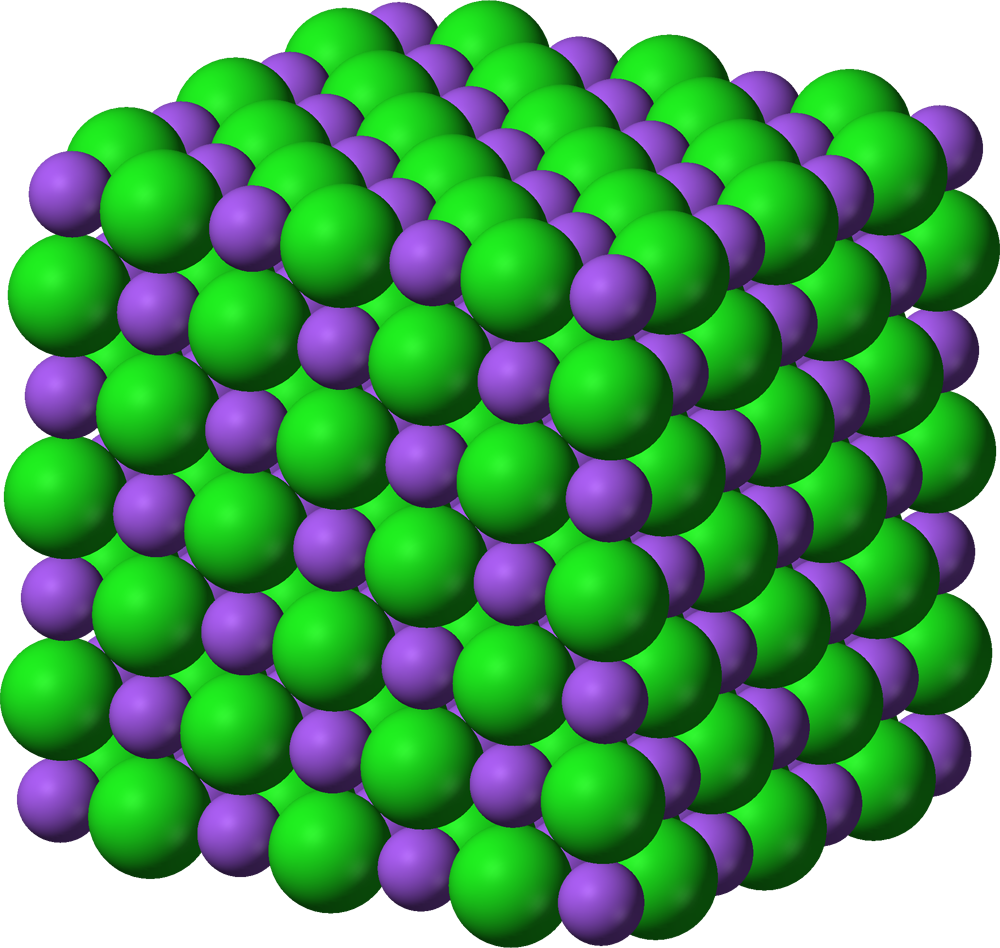
\includegraphics[width=4cm]{Sodium-chloride-3D-ionic.png}
\end{center}
includes the translations of space that move each green chlorine atom and purple natrium atom to its neighbor, up, down, left, right, forward or back, and mirror reflections around the coordinate planes through the origin, where we put the origin in the middle of any one of these atoms, and also the transformations given by permuting the order of the variables \(x,y,z\) of each coordinate axis.
\end{example}
\begin{example}
Every \(2 \times 2\) matrix 
\[
A=
\begin{pmatrix}
a & b \\
c & d
\end{pmatrix}
\]
(with entries from any chosen field) determines a \emph{linear transformation}\define{transformation!linear}\define{linear transformation}:
\[
\begin{pmatrix}
x \\
y
\end{pmatrix}
\mapsto
A
\begin{pmatrix}
x \\
y
\end{pmatrix}
=
\begin{pmatrix}
a & b \\
c & d
\end{pmatrix}
\begin{pmatrix}
x \\
y
\end{pmatrix}
=
\begin{pmatrix}
ax + by \\
cx + dy
\end{pmatrix}
\]
of the plane.
Similarly, a square matrix \(A\), say \(n \times n\), determines a linear transformation of \(n\)-dimensional Euclidean space.
A linear transformation is a bijection just when the associated matrix \(A\) is invertible, i.e. just when \(A\) has nonzero determinant.\SubIndex{determinant}
The invertible \(n \times n\) matrices form a transformation group \(G\), of linear transformations of \(n\)-dimensional Euclidean space.
\end{example}
\begin{example}
Take \(X\) to be the set of numbers \(\set{1,2,3,4}\).
The \emph{symmetric group}\define{symmetric group} on 4 letters is the group \(G\) of all permutations of \(X\).
The terminology ``on 4 letters'' reminds us that we could just as well have taken \(X=\set{a,b,c,d}\) to consist of any 4 distinct elements, and then we would get essentially the same story, just relabelling.
It is convenient notation to write a permutation of finite sets as, for example,
\[
\begin{pmatrix}
1 & 2 & 3 & 4 \\
2 & 3 & 1 & 4
\end{pmatrix}
\]
to mean the map \(f\) so that \(f(1)=2\), \(f(2)=3\), \(f(3)=1\) and \(f(4)=4\), i.e. reading down from the top row as the input to \(f\) to the entry underneath as the output of \(f\).
It is often understood that the first row is just \(1 \ 2 \ 3 \ 4\) or some such, so we can just write down the second row: \(2 \ 3 \ 1 \ 4\), to display the permutation.
\end{example}

\begin{problem}{groups:compose.permutation}
What is are the permutations \(g \circ f\) and \(f \circ g\) where \(g\) is
\[
2 \ 3 \ 1 \ 4
\]
and \(f\) is
\[
3 \ 1 \ 2 \ 4?
\]
\end{problem}

Another notation for permutations: the \emph{cycle}\define{cycle} \((1 3 4 2)\) means the permutation that takes \(1\) to \(3\), \(3\) to \(4\), \(4\) to \(2\) and \(2\) to \(1\), reading from left to right.
More generally, the cycle \((a_1 a_2 \dots a_k)\) is the permutation taking \(a_1\) to \(a_2\), \(a_2\) to \(a_3\), and so on, and taking \(a_k\) to \(a_1\).
So \((2 3 1 4)\) takes \(3\) to \(1\).
By definition, if we have a number \(x\) which is not among these various \(a_1, a_2, \dots, a_k\), then the cycle \((a_1 a_2 \dots a_k)\) fixes the number \(x\):
\((2 3 5 4)\) takes \(1\) to \(1\).
Two cycles \((a_1 a_2 \dots a_k)\) and \((b_1 b_2 \dots b_{\ell})\) are \emph{disjoint}\define{cycle!disjoint} if none of the \(a_i\) occur among the \(b_j\) and vice versa.
So 
\[
(1 4 5 2) \text{ is disjoint from } (3 6),
\]
but
\[
(1 3 5 2) \text{ is not disjoint from } (3 6)
\]
since they both have \(3\) in them.
We can write the identity permutation as \(()\).
Note that any cycle of length 1 is also the identity transformation: \((2)=(1)=()\), since \((2)\) takes \(2\) to \(2\), and fixes everything else.
If two permutations \(f\) and \(g\) can be expressed as disjoint cycles, then \(fg=gf\), since each fixes all of the letters moved by the other.

Sage knows how to multiply cycles:
\begin{sageblock}
G = SymmetricGroup(5)
sigma = G("(1,3) (2,5,4)")
rho = G([(2,4), (1,5)])
rho^(-1) * sigma * rho
\end{sageblock}
prints \(\sage{rho^(-1) * sigma * rho}\).

\begin{theorem}
Every permutation of the elements of a finite set is expressed as a product of disjoint cycles, uniquely except for the order in which we write down the cycles, which can be arbitrary.
\end{theorem}
\begin{proof}
Suppose our finite set is \(1,2,\dots,n\).
Our permutation \(f\) takes \(1\) to some number \(f(1)\), takes that number to some other number \(f(f(1))\), and so on, and eventually (because there are finitely many), if we repeat it enough times we cycle back to a number we have seen before.
Suppose that this first happens at the \(k\)-th step.
Writing \(f^21\) to mean \(f \circ f(1)\), not multiplication but composition, we are saying that \(f^k 1\) must already be among \(1,f1,\dots,f^{k-1}1\), say \(f^k 1=f^{\ell} 1\) for some \(0 \le \ell < k\).
Suppose that we pick \(k\) the smallest possible
Since \(f\) is a bijection, if \(\ell > 0\) we apply \(f^{-1}\) to both sides of \(f^k 1=f^{\ell} 1\) to find a smaller value of \(k\), a contradiction.
So \(\ell=0\), i.e. \(f^k1=1\) is our first repeat.
So we have a cycle \((1 \ f1 \ \dots \ f^{k-1}1)\).
But that cycle might not exhaust the whole of \(f\), since there might be some other numbers among \(1,2,\dots,n\) not among the elements of this cycle.

Take the smallest one, say \(b\).
Since \(f\) is a bijection, if any number from \(b,fb,f^2b,\dots\) is also in the cycle \((1 \ f1 \ f^21 \ \dots \ f^{k-1} 1\), we can apply \(f^{-1}\) to both sides as many times as we need to get that \(b\) is already in that cycle, a contradiction.
By the same argument above, replacing \(1\) by \(b\), we get another cycle \((b \ fb \ \dots \ f^{\ell -1}b)\) disjoint from the first.
Continue in this way by induction to express \(f\) as a product of disjoint cycles.
This expression is unique, since each cycle is precisely built from applying \(f\) repeatedly to any element until a cycle forms, so any two such expressions have exactly the same cycle through any element.
\end{proof}

For example, in cycle notation
\[
\begin{pmatrix}
1 & 2 & 3 & 4 \\
2 & 3 & 1 & 4
\end{pmatrix}
=(1 2 3)
\]
and
\[
\begin{pmatrix}
1 & 2 & 3 & 4 & 5 \\
3 & 4 & 1 & 5 & 2 
\end{pmatrix}
=(1 3)(2 4 5).
\]

\begin{problem}{groups:count.perms}
Prove that any set with \(n\) elements has \(n!\) permutations, in several ways: by counting 
\begin{enumerate}
\item how many places to move \(1\) to, and then how many places there are left to move \(2\) to, and so on,
\item the number of places to stick object \(n\) in between the elements of any given permutation \(a_1 a_2 \dots a_{n-1}\) of the numbers \(1,2,\dots,n-1\), say as \(n a_1 a_2 \dots a_{n-1}\) or \(a_1 n a_2 \dots a_{n-1}\) or \(a_1 a_2 n \dots a_{n-1}\) and so on, for example: given the permutation
\[
3 \ 1 \ 2
\]
of the numbers \(1,2,3\), we can put \(4\) in there as
\[
4 \ 3 \ 1 \ 2, \quad 3 \ 4 \ 1 \ 2, \quad 3 \ 1 \ 4 \ 2, \text{ or } \quad 3 \ 1 \ 2 \ 4.
\]
\item the number of ways to put at the end of a given permutation \(a_1 a_2 \dots a_{n-1}\) some number \(b\) from among 
\[
b=\frac{1}{2}, 1+\frac{1}{2}, \dots, n-\frac{1}{2},
\]
for example into the permutation \(3 \ 1 \ 2\) we stick
\[
3 \ 1 \ 2 \ \frac{1}{2}, \quad \text{ or }
3 \ 1 \ 2 \ \frac{3}{2}, \quad \text{ or }
3 \ 1 \ 2 \ \frac{5}{2}, \quad \text{ or }
3 \ 1 \ 2 \ \frac{7}{2}
\]
and then replace the numbers in the list by integers from \(1,2,\dots,n\), but in the same order:
\[
4 \ 2 \ 3 \ 1, \quad \text{ or }
4 \ 1 \ 3 \ 2, \quad \text{ or }
4 \ 1 \ 2 \ 3, \quad \text{ or }
3 \ 1 \ 2 \ 4.
\]
\item
the possible disjoint cycles.
\end{enumerate}
\end{problem}


Sage knows all of the permutations of small symmetric groups, and will print them out for you in cycle notation:
\begin{sageblock}
H = DihedralGroup(6)
H.list()
\end{sageblock}
yields
\[
\begin{array}{lll}
               , & (1,6)(2,5)(3,4), & (1,2,3,4,5,6), \\ 
     (1,5)(2,4), & (2,6)(3,5),      & (1,3,5)(2,4,6), \\ 
(1,4)(2,3)(5,6), & (1,6,5,4,3,2),   & (1,4)(2,5)(3,6), \\ 
(1,2)(3,6)(4,5), & (1,5,3)(2,6,4),  & (1,3)(4,6)
\end{array}
\]
where the identity element is the blank space at the start.

\section{Groups}

Each symmetry of an equilateral triangle in the plane permutes the vertices.
If we label the vertices, say as \(1,2,3\), then every permutation of the labels \(1,2,3\) occurs from a unique symmetry of the triangle.
So the symmetries of the equilateral triangle correspond to the permutations of the labels, i.e. the symmetry group of the equilateral triangle is, in some sense, the same as the symmetric group on three letters.
It is this notion of correspondence that leads us to see that two transformation groups can be ``the same'' while they are transforming very different sets; in our example, the symmetries of the equilateral triangle transform the infinitely many points of the triangle, while the permutations of three letters transform a set of three letters.
In order to say what is ``the same'' in the two transformation groups, we need a more abstract concept of group.

A \emph{group}\define{group} is a set \(G\) so that
\begin{enumerate}
\item 
To any elements \(a,b\) of \(G\) there is associated an element \(ab\) of \(G\), called the \emph{product} of \(a\) and \(b\).
\item
The product is associative: if \(a,b,c\) are elements of \(G\), then \((ab)c=a(bc)\), so that either expression is denoted as \(abc\).
\item
There is an identity element: some element \(1\) of \(G\), so that \(a1=1a=a\) for any element \(a\) of \(G\).
\item
Every element is invertible: if \(a\) is an element of \(G\), there is an element, denoted \(a^{-1}\), of \(G\) for which \(aa^{-1}=a^{-1}a=1\).
\end{enumerate}

\begin{example}
Nonzero rational numbers form a group \(G\) under usual multiplication, where \(a^{-1}\) means the reciprocal of any rational number \(a\).
Note that \(0\) does not have a reciprocal, so we have to remove it.
\end{example}
\begin{example}
Nonzero elements of any field form a group \(G\) under usual multiplication, where \(a^{-1}\) means the reciprocal of any element \(a\).
Note that \(0\) does not have a reciprocal, so we have to remove it.
\end{example}
\begin{example}
Any transformation group \(G\) is a group, using composition of transformations as its product, and the identity transformation as its identity element.
In particular, as examples of groups: the symmetry groups of geometric figures, the group of invertible matrices (under matrix multiplication), the symmetry group on some letters, the group of rotations of the Euclidean plane, and the group of rotations of Euclidean space.
\end{example}

It is easier to check if a collection of transformations forms a transformation group than to check if some abstract product operation forms a group; almost all of our examples of groups will be transformation groups in some obvious way.

Two elements \(a,b\) of a group \emph{commute}\define{commuting} if \(ab=ba\).
A group is \emph{abelian}\define{abelian} if any two elements of the group commute.

\begin{example}
Nonzero rational numbers form an abelian group under usual multiplication.
\end{example}
\begin{example}
Nonzero elements of any field form an abelian group under usual multiplication.
\end{example}
\begin{example}
Invertible \(2 \times 2\) matrices, with entries drawn from some chosen field, form an non-abelian group under usual matrix multiplication.
\end{example}
\begin{example}
The symmetries of the equilateral triangle form a non-abelian group: if we rotate by \(120\si{\degree}\) and the reflect across an angle bisector, we get a different result than if we first reflect across that bisector and then rotate.
\end{example}


\begin{problem}{groups:associativity}
Prove that, for any elements \(a,b,c,d\) of a group \(G\), 
\[
a(b(cd))=(ab)(cd)=((ab)c)d.
\]
Generalize by induction to prove that parentheses are not needed in expressions of any length.
\end{problem}

\begin{problem}{groups:powers}
For any element \(a\) of a group \(G\), define \(a^0\) to mean \(1\), and define by induction \(a^{n+1}=aa^n\).
Prove by induction that \(a^ma^n=a^{m+n}\) for an integers \(m,n\).
\end{problem}

\begin{problem}{groups:id.unique}
Suppose that \(1,1'\) are two elements of a group \(G\), and that \(a1=1a=a\) and also that \(a1'=1'a=a\) for any element \(a\) of the group \(G)\).
Prove that \(1=1'\).
\end{problem}

\begin{problem}{groups:cancel}
Given elements \(a, b\) of a group \(G\), prove that the equation \(ax=b\) has a unique solution \(x\) in \(G\).
Prove also that the equation \(ya=b\) has a unique solution \(y\) in \(G\).
\end{problem}

\begin{problem}{groups:inverse.order}
Prove that \((ab)^{-1}=b^{-1}a^{-1}\) for any elements \(a,b\) of any group.
\end{problem}

\begin{problem}{groups:idempt}
Suppose that \(x\) belongs to a group \(G\) and that \(x^2=x\).
Prove that \(x=1\).
\end{problem}

\begin{problem}{groups:rats.divide}
Prove that the set of nonzero rational numbers, with product operation defined as usual division, do not form a group.
(It might help to write the operation is some funny notation like \(a \star b\), instead of \(ab\), which easily gets confused with multiplication.)
\end{problem}



\section{Additive notation}

When a group is abelian, it is often preferred to write the group operation not as \(ab\) but instead as \(a+b\), and the identity element as \(0\) rather than \(1\), and the inverse as \(-a\) rather than \(a^{-1}\).

\begin{example}
The set of integers form an abelian group, where the group operation is usual addition.
\end{example}
\begin{example}
Any field is an abelian  group, where the group operation is usual addition.
\end{example}
\begin{example}
The set of \(2 \times 2\) matrices, with integer entries form an abelian  group, where the group operation is usual addition.
The same for rational entries, real entries, complex entries, entries drawn from any field, and for \(2 \times 3\) matrices, and so on.
\end{example}
\begin{example}
The rotations of the plane around the origin form an abelian group, writing each rotation in terms of its angle of rotation, and using addition of angles, i.e. composition of rotations, as the group operation.
(Careful: the rotations of Euclidean 3-dimensional space form a non-abelian group.)
\end{example}


\begin{problem}{groups:tgt}
Define an operation on real numbers \(b,c\) by
\[
b \star c = \frac{b+c}{1-bc}.
\]
With this operation, are the real numbers an abelian group?
Consider the collection consisting of all numbers of the form \(b=\frac{3p}{q}\) with \(p, q\) integers so that \(3\) does not divide \(q\).
Is this collection of numbers a group under this operation?
\end{problem}

\begin{problem*}{groups:polynomial.group}
Suppose that we turn the real numbers \(\R{}\) into a group using some weird multiplication, say \(x*y=p(x,y)\) and with some identity element \(x_0\).
Suppose that \(p(x,y)\) is a polynomial.
Prove that \(p(x,y)\) is given by the formula \(p(x+x_0,y+x_0)=x+y+x_0\).
\end{problem*}
\begin{answer}{groups:polynomial.group}
Suppose first that \(x_0=0\).
For any \(y \in \R{}\), let \(p_y\) be the polynomial \(p(x,y)\). 
Let \(y'\) be the inverse of \(y\) in the group.
Then \(p_y \circ p_{y'}(x) = x\), so that \(\degree{p_y} \degree{p_{y'}} = 1\). 
So \(p(x,y)\) has degree \(1\) in \(x\), and by the same argument has degree 1 in \(y\).
So \(p(x,y)=a+bx+cy+dxy\) for some numbers \(a,b,c,d\). 
Since \(p(x,0)=x\) and \(p(0,y)=y\), \(a=0\) and \(b=c=1\). 

If \(d\ne 0\), then pick \(x_0\) to be the unique solution to \(1+dx=0\), i.e. \(x_0\defeq-1/d\).
Let \(x_0'\) be the inverse of \(x_0\) in the group.
The map taking \(y\) to \(x_0*y = p(x_0,y)\) has inverse map \(y \mapsto x_0'*y\), so is a bijection.
But
\begin{align*}
x_0*y&=p(x_0,y),\\
&=x_0+y+dx_0y,\\
&=x_0+y(1+dx_0),\\
&=x+0,
\end{align*}
is constant, not a bijection, a contradiction, so \(d=0\), i.e. \(p(x,y)=x+y\).

If the identity element is \(x_0\) instead, then the operation \(x\otimes y=p(x+x_0,y+x_0)-x_0\) is a new group operation with identity element \(0\), so \(p(x+x_0,y+y_0)=x+y+x_0\).
\end{answer}


Sage knows many finite groups, and can say whether they are abelian:
\begin{sageblock}
H = SymmetricGroup(6)
H.is_abelian()
\end{sageblock}
yields \(\sage{H.is_abelian()}\).

\section{Multiplication tables}

If a group \(G\) is finite (i.e. has finitely many elements), we let \(|G|\)\Notation{.G.}{\orderForNotationIndex{G}}{order of group} be the number of elements of \(G\), called the \emph{order}\define{order} of \(G\).
We can then write a \emph{multiplication table}\define{multiplication table}, with rows representing some element \(x\), columns some element \(y\), and entries \(xy\)
For example, if a group \(G\) has 2 elements, say \(1\) and \(a\), then it is easy to see that \(a^2=1\) so the multiplication table must be
\[
\begin{array}{c|cc}
  &  1 & a \\ \hline
1 &  1 & a \\
a &  a & 1
\end{array}
\]

\begin{problem}{groups:order.three}
Prove that any group \(G\) of order 3 has (in some labelled of its elements) the multiplication table
\[
\begin{array}{c|ccc}
  &  1 & a & b \\ \hline
1 &  1 & a & b \\
a &  a & b & 1 \\
b &  b & 1 & a
\end{array}
\]
\end{problem}

If \(G\) and \(H\) are two groups, their \emph{product}\define{product} is the group \(G \times H\) whose elements are pairs \((g,h)\) of elements \(g\) of \(G\) and \(h\) of \(H\), with product
\[
(g_1,h_1)(g_2,h_2)=(g_1g_2,h_1h_2)
\]
and identity element \((1,1)\).
Given a multiplication table for \(G\) and one for \(H\), we can make one for \(G \times H\) by taking each row \(a\) and column \(b\) entry \(ab\) for \(G\), and each row \(x\) and column \(y\) entry \(xy\) for \(H\), and writing out \((a,x)\) as a row for \(G \times H\), \((b,y)\) as a row for \(G \times H\), and \((ab,xy)\) as entry.
For example, if \(G=H\) are both the group of order 2 above, then \(G \times H\) has multiplication table:
\[
\begin{array}{c|cccc}
      &     1 & (a,1) & (1,a) & (a,a) \\ \hline
    1 &     1 & (a,1) & (1,a) & (a,a) \\
(a,1) & (a,1) &     1 & (a,a) & (1,a) \\
(1,a) & (1,a) & (a,a) &     1 & (a,1) \\
(a,a) & (a,a) & (1,a) & (a,1) &     1
\end{array}
\]

An \emph{isomorphism}\define{isomorphism!of groups}\define{group!isomorphism} \(\phi \colon G \to H\) is a bijection between elements of two groups \(G\) and \(H\) so that \(\phi(xy)=\phi(x)\phi(y)\): \(\phi\) preserves multiplication.
If there is some isomorphism between two groups, they are \emph{isomorphic}, and for all purposes of algebra we can treat them as being the same group.

\begin{example}
In problem~\vref{problem:groups:order.three}, we saw that all groups of order 3 are isomorphic.
\end{example}
\begin{example}
The remainders modulo \(4\) form a group \(G_1\), under addition as the group operation.
The set of complex numbers \(G_2=\set{1,-1,i,-i}\) form a group under multiplication.
\end{example}
\begin{example}
The matrices
\[
\begin{pmatrix}
1 & 0 \\
0 & 1
\end{pmatrix},
\begin{pmatrix}
0 & 1 \\
-1 & 0
\end{pmatrix},
\begin{pmatrix}
-1 & 0 \\
0 & -1
\end{pmatrix},
\begin{pmatrix}
0 & -1 \\
1 & 0
\end{pmatrix}
\] 
form a group \(G_3\) under multiplication.
All of these groups are isomorphic.
For example, map \(0 \mapsto 1\), \(1 \mapsto i\), \(2 \mapsto -1\), \(3 \mapsto -i\) to map \(G_1 \to G_2\).
\end{example}
\begin{example}
Let \(G\) be the group of order \(2\) we found above and \(H\) the group of remainders modulo 4.
The groups \(G \times G\) and \(H\) are both of order \(4\), but they are \emph{not} isomorphic, because \(H\) contains the element \(1\) and every element of \(H\) is expressed in terms of \(1\) as precisely one of the 4 elements
\[
1,\ 1+1,\ 1+1+1,\ 1+1+1+1.
\]
So if \(G\) (in multiplication notation!) were isomorphic to \(H\), we would have to find some element \((x,y)\) of \(G\) so that the 4 elements 
\[
(x,y),(x,y)^2,(x,y)^3,(x,y)^4
\] 
constitute the whole of \(G\).
Check the multiplication table above to see that every \((x,y)\) in \(G\) satisfies \((x,y)^2=(1,1)\).
\end{example}

Sage knows the multiplication tables of many groups.
The \emph{dihedral group}\define{dihedral group} \(D_n\)\Notation{Dn}{D_n}{the dihedral group} is the symmetry group of a regular polygon with \(n\) equal sides and angles.
If we type
\begin{sageblock}
H = DihedralGroup(6)
H.cayley_table()
\end{sageblock}
we see the multiplication table:
\[
{\setlength{\arraycolsep}{2ex}
\begin{array}{r|*{12}{r}}
\multicolumn{1}{c|}{\cdot}&a&b&c&d&e&f&g&h&i&j&k&l\\\hline
{}a&a&b&c&d&e&f&g&h&i&j&k&l\\
{}b&b&a&e&h&c&j&k&d&l&f&g&i\\
{}c&c&d&f&g&b&i&l&a&k&e&h&j\\
{}d&d&c&b&a&f&e&h&g&j&i&l&k\\
{}e&e&h&j&k&a&l&i&b&g&c&d&f\\
{}f&f&g&i&l&d&k&j&c&h&b&a&e\\
{}g&g&f&d&c&i&b&a&l&e&k&j&h\\
{}h&h&e&a&b&j&c&d&k&f&l&i&g\\
{}i&i&l&k&j&g&h&e&f&a&d&c&b\\
{}j&j&k&l&i&h&g&f&e&d&a&b&c\\
{}k&k&j&h&e&l&a&b&i&c&g&f&d\\
{}l&l&i&g&f&k&d&c&j&b&h&e&a\\
\end{array}}
\]
where \(a\) is the identity element.


\section{Cyclic groups}

A group \(G\) is \emph{cyclic}\define{cyclic} if it consists of the powers of a single element \(x\), i.e. \(G\) consists of the powers \(x^n\) for integers \(n\).
For example, the integers (written additively) are generated by multiplies of \(1\), as is the group of remainders modulo some integer \(n \ge 0\).

\begin{theorem}\label{theorem:cyclic.groups}
Every cyclic group \(G\) is isomorphic to either the integers (when \(|G|=\infty\)) or to the integers modulo an integer \(n \ge 0\), when \(|G|=n\).
\end{theorem}
\begin{proof}
Suppose that \(G\) consists of the powers \(x^k\) of a single element \(x\).
Define a map \(f \colon \Z{} \to G\) by \(f(k)=x^k\).
Then clearly \(f(k+\ell)=x^{k+\ell}=x^kx^{\ell}=f(k)f(\ell)\).
If \(f\) is a bijection, then \(f\) is our isomorphism.
So suppose that \(f\) is not a bijection.
By definition, \(f\) is surjective, so \(f\) must fail to be injective, i.e. \(f(k)=f(\ell)\) for some \(k\ne \ell\), i.e. \(x^k=x^{\ell}\), i.e. \(x^{k-\ell}=0\) i.e. \(f(k-\ell)=1\).
Let \(K \subset \Z{}\) be the set of all integers \(m\) so that \(f(m)=1\).
Note that \(K\) contains zero, and \(K\) also contains some nonzero element \(k-\ell\).
If \(m\) is in \(K\) then \(x^m=1\) so \(x^{2m}=1\) and so on, i.e. if \(m\) is in \(K\) then all multiples of \(m\) are in \(K\).
If \(K\) contains some integers \(b,c\), take B\'ezout coefficients \(sb+tc=g\) and then
\[
f(g)=f(sb+tc)=x^{sb+tc}=(x^b)^s(x^c)^t=1^s1^t=1.
\]
Hence \(g\) is in \(K\) as well: the greatest common divisor \(n\) of all elements of \(K\) also lies in \(K\).
But then every multiple of \(n\) also lies in \(K\).
Hence \(K\) consists precisely of all multiples of \(n\), i.e. \(K=n\Z{}\), and so \(G=\set{1,x,\dots,x^{n-1}}\) is  isomorphic to the remainders modulo \(n\), taking each remainder \(b\) to \(x^b\).
\end{proof}

The \emph{order}\define{order!group element} of an element \(a\) of a group \(G\) is the order of the cyclic group consisting of the powers \(a^k\).

\begin{problem}{groups:order.comm}
Take any two elements \(a,b\) of some group.
Prove that \(ab\) and \(ba\) have the same order.
\end{problem}


\begin{problem}{groups:order.two.comm}
Take any two elements \(a,b\) of order two in some group.
If \(ab\) also has order two, prove that \(a\) and \(b\) commute.
\end{problem}


\begin{problem}{groups:order.disjoint}
Take a permutation \(f\) of \(n\) letters \(1,2,\dots,n\), expressed as a product of disjoint cycles.
Prove that the order of \(f\) is the least common multiple of the orders of the disjoint cycles.
\end{problem}

Sage can compute the order of an element of a group:
\begin{sageblock}
G = SymmetricGroup(5)
sigma = G("(1,3) (2,5,4)")
sigma.order()
\end{sageblock}
yields \(\sage{sigma.order()}\).



\section{Graphs}

\begin{example}
Take a hexagon \(X\) in the plane and let \(G\) be its symmetry group.
Label the vertices of \(X\) in order as we travel around the vertices counterclockwise, say as \(1,2,3,4,5,6\).
\begin{center}
\documentclass[tikz]{standalone}
\usepackage{xparse}
\colorlet{curveZero}{gray!75}
\colorlet{curveOne}{blue!60}
\colorlet{curveTwo}{brown!50!gray}
\colorlet{curveThree}{green!40!gray}
\colorlet{curveFour}{red!50!gray}
\NewDocumentCommand\DrawDotInPlot{O{}mmO{}}%
{%
\fill[gray!20,draw=gray] (axis cs:{#2},{#3}) circle (1.3pt) node[above,black,#4] {\(#1\)};%
}%
\NewDocumentCommand\DrawDot{O{}mmO{}}%
{%
\fill[gray!20,draw=gray] ({#2},{#3}) circle (1.3pt) node[above,black,#4] {\(#1\)};%
}%
\NewDocumentCommand\DrawNode{O{}m}%
{%
\fill[gray!20,draw=gray] (#2) circle (1.3pt) node[above,black] {\(#1\)};%
}%
\colorlet{axisColor}{gray!50}
\tikzstyle{shapeZero}=[fill=curveZero,opacity=.4]
\tikzstyle{shapeOne}=[fill=curveOne,opacity=.4]
\tikzstyle{shapeTwo}=[fill=curveTwo,opacity=.4]
\tikzstyle{shapeThree}=[fill=curveThree,opacity=.4]
\tikzstyle{groupElementLabel}=[minimum size=2.4em]
\tikzstyle{groupElement}=[minimum size=2.4em,shapeZero,draw=curveZero]
\tikzstyle{cosetOne}=[minimum size=2.4em,shapeOne,draw=curveOne]
\tikzstyle{cosetTwo}=[minimum size=2.4em,shapeTwo,draw=curveTwo]


\begin{document}
\begin{tikzpicture}
\newdimen\Radi
\Radi=0.8cm
    \begin{scope}[yshift=-3\Radi]
        \fill[shapeZero,draw=curveZero] (0:\Radi) \foreach \x in {1,...,6} {
                -- ({60*\x}:\Radi)
            }-- cycle (90:\Radi);
        \draw[white] (0:\Radi) \foreach \x in {1,...,6} {
                -- ({60*\x}:{1.14*\Radi}) node[black] {$\x$}
            }-- cycle (90:\Radi);
    \end{scope}
\end{tikzpicture}
\end{document}

\end{center}
Any symmetry moves \(1\) to one of the six vertices, and moves \(2\) to a next door neighbor vertex.
We can draw the vertices of the hexagon twice, one for drawing where \(1\) is taken to, and once again to represent whether \(2\) is taken to the vertex counterclockwise from \(1\) or clockwise.
\begin{center}
\documentclass[tikz]{standalone}
\begin{document}
% Radius of regular polygons
\begin{tikzpicture}
\newdimen\Radi
\Radi=0.8cm
    % Indicate the boundary of the regular polygons
%    \draw [thin,black!20] circle (\Radi) ;
%    \fill[black!20] circle (2pt);
%    \draw (0:\Radi) \foreach \x in {120,240} {
%            -- (\x:\Radi)
%        } -- cycle (90:\Radi) node[above] {$n=3$} ;
%    \draw[xshift=2.5\Radi] (0:\Radi) \foreach \x in {90,180,...,359} {
%            -- (\x:\Radi)
%        } -- cycle (90:\Radi) node[above] {$n=4$} ;
%    \draw[xshift=5.0\Radi] (0:\Radi) \foreach \x in {72,144,...,359} {
%            -- (\x:\Radi)
%        } -- cycle (90:\Radi) node[above] {$n=5$} ;
        \foreach \x in {1,...,6} { %60,120,...,359} {
                \fill ({\Radi*cos(60*\x)},{\Radi*sin(60*\x)}) circle (1.2pt); % \node{\(b^{\x}c\)};
                \fill ({1.5*\Radi*cos(60*\x)},{1.5*\Radi*sin(60*\x)}) circle (1.2pt); % \node{\(b^{\x}c\)};
		}
            
%        % 360/7 = 51.4286 For PGF v < 1.18 we have to round to the nearest
%        % integer. Newer version support fractional angle values.
%        % For a more accurate result use the sequence
%        % {51, 103, 154, 206, 257, 309}
%        %
%        \draw[xshift=2.5\Radi] (0:\Radi) \foreach \x in {51.4286,102.8571,...,359} {
%                -- (\x:\Radi)
%            }-- cycle (90:\Radi) node[above] {$n=7$} ;
%        \draw[xshift=5.0\Radi] (0:\Radi) \foreach \x in {45,90,...,359} {
%                -- (\x:\Radi)
%            } -- cycle (90:\Radi) node[above] {$n=8$} ;
%    \draw[yshift=-6.0\Radi] (0:\Radi) \foreach \x in {10,20,...,359} {
%            -- (\x:\Radi)
%        } -- cycle (90:\Radi) node[above] {$n=36$} ;
\end{tikzpicture}
\end{document}

\end{center}
In a sense, this is a picture of the group, since every element of the group is completely determined once we know where vertices \(1\) and \(2\) go: the rest are then in order cyclically around the hexagon.
Let \(b\) be rotation of the hexagon by \(60\si{\degree}\), and let \(c\) be reflection of the hexagon across the axis of symmetry through vertex \(1\).
Label the elements of the group according to how they move vertices \(1\) and \(2\), i.e. how much of \(b\) and \(c\) they contain:
\begin{center}
\documentclass[tikz]{standalone}
\begin{document}

\begin{tikzpicture}
% Radius of regular polygons
\newdimen\Radi
\Radi=1cm
    % Indicate the boundary of the regular polygons
%    \draw [thin,black!20] circle (\Radi) ;
%    \fill[black!20] circle (2pt);
%    \draw (0:\Radi) \foreach \x in {120,240} {
%            -- (\x:\Radi)
%        } -- cycle (90:\Radi) node[above] {$n=3$} ;
%    \draw[xshift=2.5\Radi] (0:\Radi) \foreach \x in {90,180,...,359} {
%            -- (\x:\Radi)
%        } -- cycle (90:\Radi) node[above] {$n=4$} ;
%    \draw[xshift=5.0\Radi] (0:\Radi) \foreach \x in {72,144,...,359} {
%            -- (\x:\Radi)
%        } -- cycle (90:\Radi) node[above] {$n=5$} ;
        \foreach \x in {1,...,5} { %60,120,...,359} {
                \node[circle,minimum size=2.5em,fill=blue!20] at ({\Radi*cos(60*\x)},{\Radi*sin(60*\x)}) {\(b^{\x}c\)};
                \node[circle,minimum size=2.5em,fill=blue!20] at ({2*\Radi*cos(60*\x)},{2*\Radi*sin(60*\x)}) {\(b^{\x}\)};
		}
        \node[circle,minimum size=2.5em,fill=blue!20] at ({\Radi},{0}) {\(c\)};
        \node[circle,minimum size=2.5em,fill=blue!20] at ({2*\Radi},{0}) {\(1\)};        
            
%        % 360/7 = 51.4286 For PGF v < 1.18 we have to round to the nearest
%        % integer. Newer version support fractional angle values.
%        % For a more accurate result use the sequence
%        % {51, 103, 154, 206, 257, 309}
%        %
%        \draw[xshift=2.5\Radi] (0:\Radi) \foreach \x in {51.4286,102.8571,...,359} {
%                -- (\x:\Radi)
%            }-- cycle (90:\Radi) node[above] {$n=7$} ;
%        \draw[xshift=5.0\Radi] (0:\Radi) \foreach \x in {45,90,...,359} {
%                -- (\x:\Radi)
%            } -- cycle (90:\Radi) node[above] {$n=8$} ;
%    \draw[yshift=-6.0\Radi] (0:\Radi) \foreach \x in {10,20,...,359} {
%            -- (\x:\Radi)
%        } -- cycle (90:\Radi) node[above] {$n=36$} ;
\end{tikzpicture}
\end{document}

\end{center}
Multiplication of each element by \(b\) on the left, i.e. \(x \mapsto bx\), spins the hexagon around to right.
\begin{center}
\documentclass[tikz]{standalone}
\usepackage{xparse}
\colorlet{curveZero}{gray!75}
\colorlet{curveOne}{blue!60}
\colorlet{curveTwo}{brown!50!gray}
\colorlet{curveThree}{green!40!gray}
\colorlet{curveFour}{red!50!gray}
\NewDocumentCommand\DrawDotInPlot{O{}mmO{}}%
{%
\fill[gray!20,draw=gray] (axis cs:{#2},{#3}) circle (1.3pt) node[above,black,#4] {\(#1\)};%
}%
\NewDocumentCommand\DrawDot{O{}mmO{}}%
{%
\fill[gray!20,draw=gray] ({#2},{#3}) circle (1.3pt) node[above,black,#4] {\(#1\)};%
}%
\NewDocumentCommand\DrawNode{O{}m}%
{%
\fill[gray!20,draw=gray] (#2) circle (1.3pt) node[above,black] {\(#1\)};%
}%
\colorlet{axisColor}{gray!50}
\tikzstyle{shapeZero}=[fill=curveZero,opacity=.4]
\tikzstyle{shapeOne}=[fill=curveOne,opacity=.4]
\tikzstyle{shapeTwo}=[fill=curveTwo,opacity=.4]
\tikzstyle{shapeThree}=[fill=curveThree,opacity=.4]
\tikzstyle{groupElementLabel}=[minimum size=2.4em]
\tikzstyle{groupElement}=[minimum size=2.4em,shapeZero,draw=curveZero]
\tikzstyle{cosetOne}=[minimum size=2.4em,shapeOne,draw=curveOne]
\tikzstyle{cosetTwo}=[minimum size=2.4em,shapeTwo,draw=curveTwo]


\begin{document}
\begin{tikzpicture}
\newdimen\Radi
\Radi=1.3cm
        \foreach \x/\n in {1/a,2/b,3/c,4/d,5/e} { 
                \node[circle,groupElement] 
                	({\n}0) 
                	at 
                	({\Radi*cos(60*\x)},{\Radi*sin(60*\x)}) {\small\(b^{\x}c\)};
                \node[circle,groupElementLabel] 
                	({\n}0) 
                	at 
                	({\Radi*cos(60*\x)},{\Radi*sin(60*\x)}) {\small\(b^{\x}c\)};
                \node[circle,groupElement] 
                	({\n}1) 
                	at 
                	({2*\Radi*cos(60*\x)},{2*\Radi*sin(60*\x)}) {\small\(b^{\x}\)};
                \node[circle,groupElementLabel] 
                	({\n}1) 
                	at 
                	({2*\Radi*cos(60*\x)},{2*\Radi*sin(60*\x)}) {\small\(b^{\x}\)};
		}
        \node[circle,groupElement] ({f}0) at ({\Radi},{0}) {\small\(c\)};
        \node[circle,groupElementLabel] ({f}0) at ({\Radi},{0}) {\small\(c\)};
        \node[circle,groupElement] ({f}1) at ({2*\Radi},{0}) {\small\(1\)};                  
        \node[circle,groupElementLabel] ({f}1) at ({2*\Radi},{0}) {\small\(1\)};                  
		\foreach \from/\to in {a/b,b/c,c/d,d/e,e/f,f/a} {
		\draw [-stealth,very thick,curveZero] ({\from}0) -- ({\to}0);
		\draw [-stealth,very thick,curveZero] ({\from}1) -- ({\to}1);
		}
\end{tikzpicture}
\end{document}

\end{center}
Multiplication of each element by \(c\) on the right, i.e. \(x \mapsto xc\), moves the inward hexagon points to the outward ones, and vice versa.
\end{example}

Elements \(g, h, \dots\) of a group \(G\) \emph{generate}\define{generators} that group if every element can be written as a product of integer powers of those elements.
If we fix some elements generating a group \(G\), the \emph{Cayley graph}\define{Cayley graph} of \(G\) (with respect to those generators) is the set of elements of \(G\), each draw as a dot, together with an arrow from one dot to another, labelled by \(g\), if the first dot is some element \(k\) and the second is \(gk\) (or \(kg\), depending on which ordering we prefer).
These pictures are almost never useful in proving results about groups, but they give us some intuition.


Sage knows the Cayley graphs (for various generators) of many groups.
If we type
\begin{sageblock}
H = DihedralGroup(6)
show(H.cayley_graph())
\end{sageblock}
we see the graph:
\begin{center}
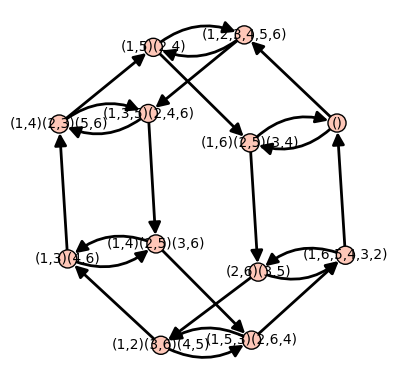
\includegraphics[width=5cm]{cayley-graph-d6.png}
\end{center}
The graph is labelled by the cycles of each element, thought of as a permutation of the vertices of the hexagon.

\section{Subgroups}

A subset \(H\) of a group \(G\) is a \emph{subgroup}\define{subgroup} if
\begin{enumerate}
\item
\(H\) contains the identity element and
\item
if \(a\) and \(b\) are elements of \(H\) then \(ab\) is also an element of \(H\), 
\item
if \(b\) is an element of \(H\) then \(b^{-1}\) is also an element of \(H\).
\end{enumerate}

It follows that \(H\) is itself a group.

\begin{example}
The even numbers are a subgroup of the integers, under usual integer addition.
\end{example}
\begin{example}
The invertible integer \(2 \times 2\) matrices are a subgroup of the invertible real \(2 \times 2\) matrices.
\end{example}
\begin{example}
If \(b\) is an element of any group \(G\), then the set of all elements of \(G\) of the form \(b^k\) for integers \(k\) is a cyclic group, the subgroup generated by \(b\).
\end{example}
\begin{example}
The real \(2 \times 2\) matrices of unit determinant form a subgroup of the group of all invertible real \(2 \times 2\) matrices, since determinants multiply.
\end{example}

\section{Cosets}

If \(S\) is any subset of a group \(G\) and \(b\) is any element of \(G\), denote by \(bS\) the set of elements of the form \(bs\) for \(s\) in \(S\), called a \emph{left translate}\define{left translate} or \emph{left coset}\define{left coset} of \(S\); if we write \emph{coset}, we mean \emph{left coset}.
Denote by \(Sb\) the set of elements of the form \(sb\) for \(s\) in \(S\), called a \emph{right translate}\define{right translate} or \emph{right coset}\define{right coset} of \(S\).
Each coset \(bS\) has the same number of elements as \(S\), since \(s \mapsto bs\) has inverse \(t \mapsto b^{-1}t\), so is a bijection.

\begin{example}
The group \(G\) of symmetries of the hexagon has a subgroup \(H\) of rotations of the hexagon.
Divide up \(G\) into \(H\)-cosets:
\begin{center}
\documentclass[tikz]{standalone}
\usepackage{xparse}
\colorlet{curveZero}{gray!75}
\colorlet{curveOne}{blue!60}
\colorlet{curveTwo}{brown!50!gray}
\colorlet{curveThree}{green!40!gray}
\colorlet{curveFour}{red!50!gray}
\NewDocumentCommand\DrawDotInPlot{O{}mmO{}}%
{%
\fill[gray!20,draw=gray] (axis cs:{#2},{#3}) circle (1.3pt) node[above,black,#4] {\(#1\)};%
}%
\NewDocumentCommand\DrawDot{O{}mmO{}}%
{%
\fill[gray!20,draw=gray] ({#2},{#3}) circle (1.3pt) node[above,black,#4] {\(#1\)};%
}%
\NewDocumentCommand\DrawNode{O{}m}%
{%
\fill[gray!20,draw=gray] (#2) circle (1.3pt) node[above,black] {\(#1\)};%
}%
\colorlet{axisColor}{gray!50}
\tikzstyle{shapeZero}=[fill=curveZero,opacity=.4]
\tikzstyle{shapeOne}=[fill=curveOne,opacity=.4]
\tikzstyle{shapeTwo}=[fill=curveTwo,opacity=.4]
\tikzstyle{shapeThree}=[fill=curveThree,opacity=.4]
\tikzstyle{groupElementLabel}=[minimum size=2.4em]
\tikzstyle{groupElement}=[minimum size=2.4em,shapeZero,draw=curveZero]
\tikzstyle{cosetOne}=[minimum size=2.4em,shapeOne,draw=curveOne]
\tikzstyle{cosetTwo}=[minimum size=2.4em,shapeTwo,draw=curveTwo]


\begin{document}
\begin{tikzpicture}
\newdimen\Radi
\Radi=1cm
        \foreach \x in {1,...,5} {
                \node[circle,cosetOne] 
                at 
                ({\Radi*cos(60*\x)},{\Radi*sin(60*\x)}) 
                {\small\(b^{\x}c\)};
                \node[circle,groupElementLabel] 
                at 
                ({\Radi*cos(60*\x)},{\Radi*sin(60*\x)}) 
                {\small\(b^{\x}c\)};
                \node[circle,cosetTwo] 
                at 
                ({1.9*\Radi*cos(60*\x)},{1.9*\Radi*sin(60*\x)}) 
                {\small\(b^{\x}\)};
                \node[circle,groupElementLabel] 
                at 
                ({1.9*\Radi*cos(60*\x)},{1.9*\Radi*sin(60*\x)}) 
                {\small\(b^{\x}\)};
		}
        \node[circle,cosetOne] 
        at 
        ({\Radi},{0}) 
        {\small\(c\)};
        \node[circle,groupElementLabel] 
        at 
        ({\Radi},{0}) 
        {\small\(c\)};
        \node[circle,cosetTwo] 
        at 
        ({1.9*\Radi},{0}) 
        {\small\(1\)};        
        \node[circle,groupElementLabel] 
        at 
        ({1.9*\Radi},{0}) 
        {\small\(1\)};        
\end{tikzpicture}
\end{document}

\end{center}
\end{example}
\begin{example}
We might draw our cosets as columns of a matrix
\begin{center}
\documentclass[tikz]{standalone}
\begin{document}

\begin{tikzpicture}
\newcommand{\Radx}{1.2}
        \foreach \x in {1,...,5} { %60,120,...,359} {
                \node[circle,minimum size=2.5em,fill=blue!20] at (1.2,{-\Radx*\x}) {\(b^{\x}c\)};
                \node[circle,minimum size=2.5em,fill=brown!40] at (0,{-\Radx*\x}) {\(b^{\x}\)};
		}
        \node[circle,minimum size=2.5em,fill=blue!20] at (1.2,0) {\(c\)};
        \node[circle,minimum size=2.5em,fill=brown!40] at (0,0) {\(1\)};        
\end{tikzpicture}
\end{document}

\end{center}
to emphasize that they are all the same size, each a copy of \(H\).
\end{example}
\begin{example}
Let \(G\) be the group of rotations and \(H\) the subgroup of those rotations which preserve a regular hexagon \(X\) around the origin.
For each angle \(\theta\), which we think of as a rotation \(g\), \(gH\) is the set of all rotations \(gh\) for \(h \in H\), i.e. geometrically the rotations which take the given hexagon \(X\) into the hexagon \(gX\).
\end{example}
\begin{example}
Let \(G\) be the group of integers under addition, and \(H\) the subgroup of multiples of \(7\), i.e. \(H\) is the set of all integers of the form \(7k\) for any integer \(k\).
Our translates in this notation have the form \(1+H, 2+H\), and so on.
The translate \(1+H\) is the set of all numbers of the form \(1+7k\) for any integer \(k\).
The translate \(2+H\) is the set of all numbers of the form \(2+7k\) for any integer \(k\), and so on.
\end{example}

\begin{lemma}\label{lemma:coset.id}
If \(x\) and \(y\) are elements of a group \(G\) and \(H\) is a subgroup of \(G\), then \(xH=yH\) just when \(y^{-1}x\) belongs to \(H\).
Any two cosets \(xH\) and \(yH\) are either disjoint: \(xH \cap yH\) empty, or equal: \(xH=yH\).
\end{lemma}
\begin{proof}
Suppose that \(xH=yH\).
Then every element \(xh\) of \(xH\) must belong to \(yH\), i.e. have the form \(yh'\) for some element \(h'\) of \(H\), so \(xh=yh'\), i.e. \(x=yh'h^{-1}\), and so \(y^{-1}x=h'h^{-1}\) is in \(H\).

Conversely, if \(y^{-1}x\) is in \(H\), then every element \(xh\) of \(xH\) has the form
\begin{align*}
xh
&=
(yy^{-1})xh, \\
&=
y(y^{-1}xh),
\\
&= yh'
\end{align*}
where \(h' = y^{-1}xh\) is in \(H\).
Similarly, every element \(yh\) of \(yH\) has the form
\begin{align*}
yh
&=
(xx^{-1})xh, \\
&=
x(x^{-1}yh),
\\
&= xh'
\end{align*}
where \(h' = x^{-1}yh = (y^{-1}x)^{-1}h\) is in \(H\).

If \(xH\) intersects \(yH\), say at \(xh=yh'\), then \(y^{-1}xh=h'\) lies in \(H\) so \(y^{-1}x\) lies in \(H\), i.e. \(xH=yH\).
\end{proof}


If \(H\) is a subgroup of a group \(G\), we let \(G/H\) be the collection of all cosets of \(H\) in \(G\).

\begin{example}
The group \(G\) of symmetries of the hexagon has a subgroup \(H\) of rotations of the hexagon.
If we  draw each coset as a column, we draw each point of \(G/H\) as a single dot underneath that column:
\begin{center}
\documentclass[tikz]{standalone}
\begin{document}

\begin{tikzpicture}
\newcommand{\Radiii}{1}
        \foreach \x in {1,...,5} {
                \node[circle,minimum size=2.5em,fill=blue!20] at (1,{-\Radiii*\x}) {\small\(b^{\x}c\)};
                \node[circle,minimum size=2.5em,fill=brown!40] at (0,{-\Radiii*\x}) {\small\(b^{\x}\)};
		}
        \node[circle,minimum size=2.5em,fill=blue!20] at (1,0) {\small\(c\)};
        \node[circle,minimum size=2.5em,fill=brown!40] at (0,0) {\small\(1\)};        
        \draw [gray!50,ultra thick] (0,{-\Radiii*5.6}) -- (1,{-\Radiii*5.6});
        \node[circle,minimum size=2.5em,fill=blue!20] at (1,{-\Radiii*6.2}) {\small\(cH\)};
        \node[circle,minimum size=2.5em,fill=brown!40] at (0,{-\Radiii*6.2}) {\small\(1H\)};        
        
\end{tikzpicture}
\end{document}

\end{center}
\end{example}
\begin{example}
Let \(G\) be the group of all rotations of the plane and \(H\) the subgroup of those rotations which preserve a regular hexagon \(X\) around the origin.
For each angle \(\theta\), which we think of as a rotation \(g\), \(gH\) is the set of all rotations \(gh\) for \(h \in H\), i.e. geometrically the rotations which take the given hexagon \(X\) into the hexagon \(gX\).
So each coset \(gH\) in \(G/H\) is identified with a rotated hexagon \(gX\), i.e. \(G/H\) is the set of all rotated hexagons \(gX\) for any rotation \(g\).
\end{example}
\begin{example}
Let \(G\) be the group of integers under addition, and \(H\) the subgroup of multiples of \(7\), i.e. \(H\) is the set of all integers of the form \(7k\) for any integer \(k\).
Our translates in this notation have the form \(1+H, 2+H\), and so on.
The translate \(1+H\) is the set of all numbers of the form \(1+7k\) for any integer \(k\), which we denote by \(\bar{1}\).
The translate \(2+H\) is the set of all numbers of the form \(2+7k\) for any integer \(k\), which we denote by \(\bar{2}\), and so on.
Of course, \(\bar{7}=\bar{0}\) is the coset of \(H\).
So \(G/H\) is the set of remainders modulo \(7\).
Each element of \(G/H\) represents ``gluing together'' all elements of \(G\) that differ by a multiple of \(H\).
\end{example}

\section{Actions}

A group \(G\) \emph{acts} on a set \(X\) if each element \(b\) of \(G\) has an associated transformation \(f_g\) of \(X\)  so that \(f_{bc} = f_b \circ f_c\) for any elements \(b, c\) of \(G\).
So then \(G\) is a transformation group of \(X\), and write \(gx\) to mean \(f_g(x)\).
The action is \emph{transitive} if any two points \(p, q\) of \(X\) are connected by some element of \(G\), i.e. \(q=gp\) for some \(g\) in \(G\).
The \emph{stabilizer} of a point \(x_0\) of \(X\) is the subset \(G^{x_0}\) of \(G\) consisting of those \(g\) in \(G\) so that \(gx_0=x_0\).
If a group \(G\) acts on two sets \(X\) and \(Y\), a map \(f \colon X \to Y\) is \emph{equivariant} if \(f(gx)=gf(x)\) for any \(x\) in \(X\) and \(g\) in \(G\).
An equivariant bijection makes two actions practically identical.

\begin{lemma}
Given a group action of a group \(G\) on a set \(X\), and an element \(x_0\) of \(X\), the stabilizer \(G^{x_0}\) of each point is a subgroup.
\end{lemma}
\begin{proof}
Clearly if \(bx_0=x_0\) and \(cx_0=x_0\) then \((bc)x_0=b(cx_0)=bx_0=x_0\) and so on.
\end{proof}

Subgroups correspond to transitive actions; geometrically it is always easier to think about actions, but algebraically it is easier to work with subgroups.
\begin{theorem}
If \(H\) is a subgroup of a group \(G\), and we let \(X=G/H\), then \(G\) acts on \(X\) transitively by \(b(cH)=(bc)H\) with stabilizer \(G^{x_0}=H\) where \(x_0\) is the coset \(1H\).
Conversely, if \(G\) acts transitively on a set \(X\), and we let \(H=G^{x_0}\), there is a unique equivariant bijection
\(
f \colon G/H \to X,
\)
so that \(f(gH)=gx_0\).
\end{theorem}
\begin{proof}
Clearly \(b(cH)=(bc)H\) is the set of elements of \(G\) of the form \(bch\) for \(h\) in \(H\).
Hence the action of \(G\) on \(G/H\) is defined.

Take any element \(gH\) of \(G/H\).
So \(gH\) is a coset.
By lemma~\vref{lemma:coset.id}, knowing only the coset \(gH\), we can determine the element \(g\), up to replacing \(g\) by \(gh\) for any \(h \in H\).
But then the expression \(gx_0\) will only change to \((gh)x_0=g(hx_0)=gx_0\), i.e. not at all.
So knowledge of the coset \(gH\) determines knowledge of \(gx_0\), i.e. \(f\) is well defined.
It is then easy to check that \(f\) is equivariant.
Since \(G\) acts transitively on \(X\), every element \(x\) of \(X\) has the form \(x=gx_0\) for some \(g\), \(f\) is surjective.
If \(f(bH)=f(cH)\) then \(bx_0=cx_0\) so \(c^{-1}bx_0 = x_0\) i.e. \(c^{-1} b\) lies in \(G^{x_0}\).
But \(H\) is by definition \(G^{x_0}\), so \(c^{-1}b\) lies in \(H\), i.e. \(bH=cH\), so \(f\) is injective.
\end{proof}



\begin{theorem}[Lagrange]\SubIndex{Lagrange, Joseph-Louis}
If \(H\) is a finite subgroup of a group \(G\) then
\[
|G/H|=\frac{|G|}{|H|}.
\]
\end{theorem}
\begin{proof}
The set \(G\) is divided up into disjoint cosets, each containing \(|H|\) elements.
\end{proof}


\begin{corollary}
The order of any finite subgroup of a group divides the order of the group.
\end{corollary}

\begin{corollary}
The order of any element of a group divides the order of the group.
\end{corollary}

\begin{corollary}
Every finite group of prime order, say order \(p\), is cyclic, isomorphic to the group of remainders modulo \(p\) under addition.
\end{corollary}
\begin{proof}
Take any element which is not the identity element, so cannot have order 1.
Since \(G\) is finite, the order of the element is finite.
Since \(|G|\) is prime, the order of the element divides this prime, so equals this prime.
\end{proof}


Take a group \(G\) acting on a set \(X\).
The \emph{orbit}\define{orbit} \(Gx\) of an element \(x\) of \(X\) is the set of all elements of \(X\) of the form \(gx\) for \(g\) in \(G\): it is where \(G\) takes \(x\).
Every orbit is, by definition, acted on transitively by \(G\), so the map \(G/G^x \to Gx\) taking \(gG^x \mapsto gx\) is an equivariant bijection.

\begin{problem}{groups:orbits.square}
If \(X\) is a hexagon in the plane, and \(G\) is the symmetry group of \(X\), what are all of the orbits of \(G\)?
\end{problem}

A \emph{fixed point}\define{fixed point} of a group \(G\) acting on a set \(X\) is a point \(x\) fixed by all elements of \(G\), i.e. \(gx=x\) for any \(g\) in \(G\).

\begin{problem}{groups:fixed.point}
If a finite group \(G\) acts on a finite set \(X\), and the order of \(X\) is coprime to the order of \(G\), prove that \(X\) contains a fixed point of the \(G\)-action.
\end{problem}



\section{Group presentations}

\begin{example}
The symmetries of an equilateral triangle can all be expressed in terms of the rotation, call it \(b\), by \(120\si{\degree}\), and the reflection, call it \(c\), about any one the axes of symmetry through one of the vertices.
Clearly \(b^3=1\), i.e. if we rotate three times by \(120\si{\degree}\), the resulting rotation by \(360\si{\degree}\) moves every point back where it started.
Similarly \(c^2=1\).
The reader can draw pictures to see that \(bc=cb^2\).
Once we have these three rules, any expression in the group in terms of \(b\) and \(c\) can be successively simplified by these three rules, to an expression in which \(c\) only appears to the first power, i.e. no \(c^2\) or \(c^{-1}\) or \(c^{-13}\) appears, and \(b\) appears only to the power \(1\) or \(2\), and \(b\) always appears after \(c\).
Hence the group is precisely
\[
1,b,c,b^2,cb,cb^2.
\]
\end{example}


Take an abstract set \(S\).
A \emph{word}\define{word} on the \emph{alphabet}\define{alphabet} \(S\) is a finite sequence of choices of element of \(S\) and integer power.
We write each word as a string of symbols
\[
s_1^{a_1} s_2^{a_2} \dots s_k^{a_k}.
\]
We allow the empty string, and write it as \(1\).
\emph{Reduce}\define{reduce} a word by deleting any \(s^0\) symbols and replacing any subword \(s^p s^q\) by \(s^{p+q}\).
The \emph{free group}\define{free!group} \(\left<S\right>\) on an alphabet \(S\) is the collection of all reduced words on \(S\).
The multiplication operation: multiply two words by writing down one after the other, called \emph{concatenation}\define{concatentation} and then reducing.
The inverse operation: write down the word in reverse order, with opposite signs for the powers.

Take an abstract set \(S\) with associated free group \(\left<S\right>\).
Take a subset \(R \subset \left<S\right>\).
The group \emph{generated} by \(S\) with \emph{relations} \(R\), denoted \(\left<S|R\right>\), is the quotient of \(\left<S\right>\) by the smallest normal subgroup containing \(R\).
The expression of a group in the form \(\left<S|R\right>\) is a \emph{presentation}\define{presentation} of the group with \emph{generators} \(S\) and \emph{relations} \(R\).

\begin{lemma}
Every map of sets \(f \colon S \to G\) to a group extends uniquely to a morphism of groups \(f \colon \left<S\right> \to G\).
It therefore extends to an injective morphism of groups \(\left<S|R\right> \to G\) where \(R\) is the set of all words 
\[
w=s_1^{a_1} s_2^{a_2} \dots s_k^{a_k}
\]
on the alphabet \(S\) for which
\[
f(s_1)^{a_1} \dots f(s_k)^{a_k} = 1.
\]
\end{lemma}

In practice, we usually write the relations not as a set \(R\), but as a collection of equations like
\[
w_1 = w_2
\]
between words.
This equation means that we require \(w_2^{-1} w_1 \in R\).

\begin{example}
The two transformations
\[
T \colon (x,y) \mapsto (x,y+1)
\]
and
\[
F \colon (x,y) \mapsto (x+1,-y)
\]
of the plane, a translation and a flip, satisfy \(TFT=F\), and generate some group \(H\), the symmetries of the wallpaper pattern:
\begin{center}
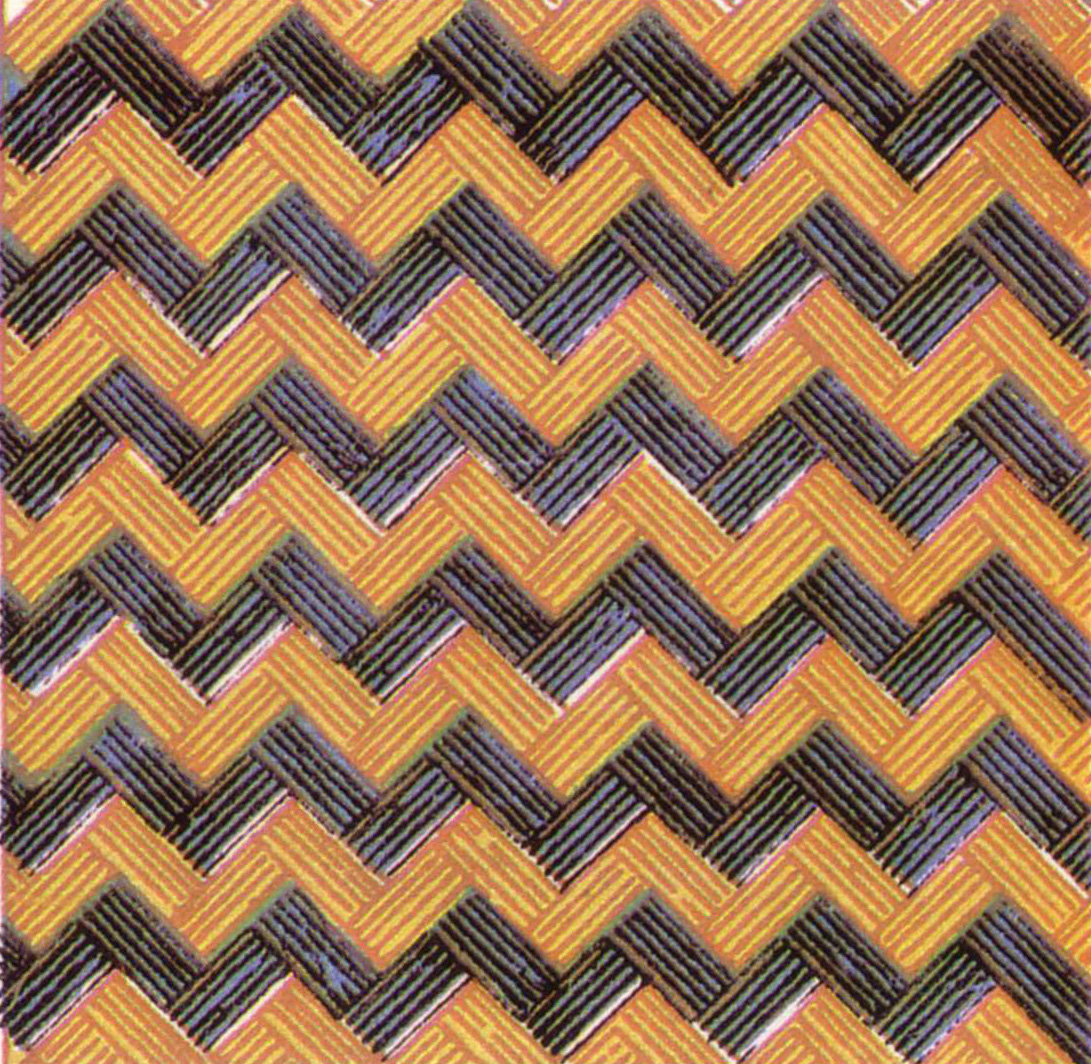
\includegraphics[width=4cm]{Wallpaper_group-pg-1.jpg}
\end{center}
Let \(G \defeq \left<f,t|tft=f\right>\); in other words \(G\) is the group generated by alphabet \(\set{t,f}\) with relation \(tft=t\), i.e. with \(R=\set{t^{-1}tft}\).
So we have a surjective map
\(
G \to H
\),
mapping \(t \mapsto T\) and \(f \mapsto F\).
Here \(t\) is a formal symbol, not an actual transformation of the plane, while \(T\) is the actual transformation.
Take any word in \(G\).
Wherever we find \(tf\) we replace it by \(ft^{-1}\).
Wherever we find \(t^{-1}f\) we replace it by \(ft\).
Wherever we find \(tf^{-1}\) we replace it by \(f^{-1}t^{-1}\).
Wherever we find \(t^{-1}f^{-1}\) we replace it by \(f^{-1}t\).
The reader can check that these are all consequences of \(tft=f\).
Therefore any word in \(G\) can be written uniquely as \(f^p t^q\).
If the corresponding transformation \(F^p T^q\) is the identity, then it fixes the origin, and so the translations of the \(x\) variable cancel each other out, i.e. \(p=0\).
But then \(T^q(x,y)=(x,y+q)\) fixes the origin just when \(q=0\).
So the only element of \(G\) mapping to the trivial transformation of the plane is \(1\).
We can see that \(G \to H\) is an isomorphism.
\end{example}



\section{Morphisms}

A \emph{morphism}\define{morphism!of groups} of groups is a map \(\phi \colon G \to H\) so that \(\phi(xy)=\phi(x)\phi(y)\): \(\phi\) preserves multiplication. 
We have seen several of these.
\begin{example}
Label the vertices of an equilateral triangle as \(1,2,3\).
Identify the group \(G\) of symmetries of the triangle with the symmetric group \(H\) on 3 letters, by taking each symmetry \(g\) of the equilateral triangle to the permutation \(h=\phi(g)\) of its vertices.
\end{example}
\begin{example}
Label the vertices of any polygon \(X\) in the plane, or polyhedron \(X\) in Euclidean 3-dimensional space, with \(n\) vertices.
Map the group \(G\) of symmetries of \(X\) to the symmetric group \(H\) on \(n\) letters, by taking each symmetry \(g\) of \(X\) to the permutation \(h=\phi(g)\) of its vertices.
This map might not be surjective.
For example, if \(X\) is a square in the plane
\begin{center}
\documentclass[tikz]{standalone}
\usepackage{xparse}
\usetikzlibrary{positioning}
\colorlet{curveZero}{gray!75}
\colorlet{curveOne}{blue!60}
\colorlet{curveTwo}{brown!50!gray}
\colorlet{curveThree}{green!40!gray}
\colorlet{curveFour}{red!50!gray}
\NewDocumentCommand\DrawDotInPlot{O{}mmO{}}%
{%
\fill[gray!20,draw=gray] (axis cs:{#2},{#3}) circle (1.3pt) node[above,black,#4] {\(#1\)};%
}%
\NewDocumentCommand\DrawDot{O{}mmO{}}%
{%
\fill[gray!20,draw=gray] ({#2},{#3}) circle (1.3pt) node[above,black,#4] {\(#1\)};%
}%
\NewDocumentCommand\DrawNode{O{}m}%
{%
\fill[gray!20,draw=gray] (#2) circle (1.3pt) node[above,black] {\(#1\)};%
}%
\colorlet{axisColor}{gray!50}
\tikzstyle{shapeZero}=[fill=curveZero,opacity=.4]
\tikzstyle{shapeOne}=[fill=curveOne,opacity=.4]
\tikzstyle{shapeTwo}=[fill=curveTwo,opacity=.4]
\tikzstyle{shapeThree}=[fill=curveThree,opacity=.4]
\tikzstyle{groupElementLabel}=[minimum size=2.4em]
\tikzstyle{groupElement}=[minimum size=2.4em,shapeZero,draw=curveZero]
\tikzstyle{cosetOne}=[minimum size=2.4em,shapeOne,draw=curveOne]
\tikzstyle{cosetTwo}=[minimum size=2.4em,shapeTwo,draw=curveTwo]


\newcounter{squareBoxCounter}
\begin{document}
\setcounter{squareBoxCounter}{0}
\NewDocumentCommand\sqrbox{mmmm}{%
\stepcounter{squareBoxCounter}%
\begin{scope}[xshift=\thesquareBoxCounter in]%
\fill[shapeZero,draw=curveZero] (0,0) rectangle (1,1);%
\node[below left=-1.3mm and -1.3mm] at (0,0) {#1};%
\node[above left=-1.3mm and -1.3mm] at (0,1) {#2};%
\node[above right=-1.3mm and -1.3mm] at (1,1) {#3};%
\node[below right=-1.3mm and -1.3mm] at (1,0) {#4};%
\end{scope}}%
\begin{tikzpicture}[scale=.5]%
\sqrbox{1}{2}{3}{4}%
\sqrbox{4}{1}{2}{3}%
\sqrbox{1}{4}{3}{2}%
\end{tikzpicture}%
\end{document}
\end{center}
no rotation or reflection will ever put \(1\) and \(2\) diagonally across from each other, because that would pull them apart to a greater distance.
\end{example}
\begin{example}
Every element \(g\) of any group \(G\) has associated a morphism
\[
\phi \colon \Z{} \mapsto G,
\]
given by \(\phi(k)=g^k\).
This map is surjective just when \(G\) is cyclic, and injective just when \(g\) has infinite order.
\end{example}

Almost everything we know about any group arises from looking at morphisms to that group and from that group.
The \emph{kernel}\define{kernel} of a morphism \(\phi \colon G \to H\) is the set of all elements \(g\) of \(G\) for which \(\phi(g)=1\), i.e. the elements ``killed'' by \(\phi\).
The \emph{image}\define{image} of a morphism \(\phi \colon G \to H\) is the set of all elements \(h\) of \(H\) for which \(h=\phi(g)\) for some \(g\) in \(G\).

\begin{problem}{groups:kernel}
Prove that the kernel of any morphism of groups \(\phi \colon G \to H\) is a subgroup of \(G\).
\end{problem}

\begin{problem}{groups:kernel.2}
Prove that the kernel of any morphism of groups \(\phi \colon G \to H\) is \(\set{1}\) just when \(\phi\) is injective.
\end{problem}

\begin{problem}{groups:image}
Prove that the image of any morphism of groups \(\phi \colon G \to H\) is a subgroup of \(H\).
\end{problem}

It seems natural to ask which subgroups arise as kernels and as images.

\begin{problem}{groups:image.2}
Prove that every subgroup \(G\) of any group \(H\) is the image of a morphism of groups \(\phi \colon G \to H\).
\end{problem}

A subgroup \(K\) of a group \(G\) is \emph{normal} if \(gKg^{-1}=K\) for any \(g\) in \(G\).

\begin{problem}{groups:rigid.motion.normal}
Every rigid motion \(f\) of three dimensional Euclidean space can be written uniquely as \(f(x)=Ax+b\) where \(A\) is an orthogonal matrix and \(b\) is a vector in three dimensional Euclidean space.
A \emph{translation} is a rigid motion \(f\) of the form \(f(x)=x+b\).
An \emph{orthogonal transformation} is a rigid motion \(f\) of the form \(f(x)=Ax\).
Let \(G\) be the group of all rigid motions three dimensional Euclidean space.
Let \(T\) be the set of all translations.
Prove that \(T\) is a normal subgroup of \(G\).
Let \(U\) be the set of all orthogonal transformations.
Prove that \(U\) is \emph{not} a normal subgroup of \(G\).
\end{problem}

\begin{theorem}
A subset \(K\) of a group \(G\) is a normal subgroup if and only if \(K\) is the kernel of some morphism \(\phi \colon G \to H\) to some group \(H\).
Indeed, if \(K\) is normal, then there is a unique group operation on \(G/K\) so that the map \(\phi \colon G \to G/K\) given by \(\phi(g)=gK\) is a group morphism with kernel \(K\).
\end{theorem}
\begin{proof}
If \(K\) is the kernel of a morphism \(\phi \colon G \to H\) to some group \(H\), then an element \(k\) of \(G\) belongs to \(K\) just when \(\phi(k)=1\).
But 
\[
\phi(gkg^{-1})
=
\phi(g)\phi(k)\phi(g)^{-1}
\]
so \(\phi(k)=1\) implies \(\phi(gkg^{-1})=1\) i.e. if \(k\) lies in \(K\) then \(gkg^{-1}\) does too.
Similarly,
\begin{align*}
\phi(k)
&=
\phi(g^{-1}g \, k \, g^{-1}g),
\\
&=
\phi(g)^{-1}\phi(g \, k \, g^{-1})\phi(g),
\end{align*}
so \(\phi(gkg^{-1})=1\) implies \(\phi(k)=1\) i.e. \(k\) lies in \(K\) just when \(gkg^{-1}\) does too.
Hence \(K\) is normal.

Suppose that \(K\) is normal.
Define on \(G/K\) the operation \((bK)(cK)=bcK\).
It is convenient to write each coset \(bK\) of \(K\) as \(\bar{b}\).
Then the operation is \(\bar{b}\bar{c}=\overline{bc}\), with identity \(\bar{1}\).
To see that this is well defined, note that knowledge of the coset \(bK\) determines \(b\) precisely up to replacing \(b\) by \(bk\) for some \(k\) in \(K\).
Hence \(\bar{b}\) determines \(b\) uniquely up to the equation \(\bar{b}=\overline{bk}\) for \(k\) in \(K\).
So given \(\bar{b}\) and \(\bar{c}\), we know \(b\) and \(c\) precisely up to replacing them with \(bk_0\) and \(ck_1\) for some \(k_0, k_1\) in \(K\).
Hence this replaces \(bc\) by
\[
bk_0 ck_1 = bc (c^{-1} k_0 c) k_1.
\]
But then taking \(K\)-cosets,
\[
\overline{bk_0 ck_1} = \overline{bc}.
\]
Hence the resulting product \(\bar{bc}\) comes out the same for \(b,c\) and for \(bk_0\) and \(ck_1\), i.e. the operation is well defined.
The kernel of this operation is the set of elements \(b\) of \(G\) for which \(\bar{b}=\bar{1}\) i.e. \(bK=K\) i.e. \(b\) in \(K\).
\end{proof}

Sage can tell you whether the subgroup \(H\) generated by some elements \(r_1,r_2,r_3\) is a normal subgroup:
\begin{sageblock}
A4 = AlternatingGroup(4)
r1 = A4("(1,2) (3,4)")
r2 = A4("(1,3) (2,4)")
r3 = A4("(1,4) (2,3)")
H = A4.subgroup([r1, r2, r3])
H.is_normal(A4)
\end{sageblock}
yields \(\sage{H.is_normal(A4)}\).

\begin{theorem}
The image of any morphism of groups \(\phi \colon G \to H\) with kernel \(K\) is isomorphic to \(G/K\) by the isomorphism
\[
\bar\phi \colon G/K \to H
\]
given by \(\bar\phi(gK)=\phi(g)\).
If \(\phi\) is onto, then \(\bar\phi\) is onto.
\end{theorem}
\begin{proof}
When we map \(g\) to \(\phi(g)\), if we replace \(g\) by \(gk\) for any \(k\) in \(K\), this replaces \(\phi(g)\) by \(\phi(gk)=\phi(g)\phi(k)=\phi(g)1=\phi(g)\).
Hence \(\bar\phi(\bar{g})=\phi(g)\) is well defined.
It is morphism of groups because \(\bar\phi(\overline{bc})=\phi(bc)=\phi(b)\phi(c)=\bar\phi(\bar{b})\bar\phi(\bar{c})\).
Its kernel is \(\set{\bar{1}}\), because \(\bar\phi(\bar{b})=1\) just when \(\phi(b)=1\) just when \(b\) is in \(K\), so just when \(\bar{b}=\bar{1}\) is the identity element of \(G/K\).
\end{proof}

Sage knows how to construct the quotient group \(G/H\):
\begin{sageblock}
A4 = AlternatingGroup(4)
r1 = A4("(1,2) (3,4)")
r2 = A4("(1,3) (2,4)")
r3 = A4("(1,4) (2,3)")
H = A4.subgroup([r1, r2, r3])
A4.quotient(H)
\end{sageblock}
yields \(\sage{A4.quotient(H)}\), meaning that the quotient group is isomorphic to the group of permutations generated by the cycle \((1 \ 2 \ 3)\).


\begin{lemma}
Suppose that \(\phi \colon G \to H\) is a morphism of groups and that \(N_G\) and \(N_H\) are normal subgroups of \(G\) and \(H\) and that \(\phi(N_G)\) lies in \(N_H\).
Then there is a unique morphism \(\bar\phi \colon G/N_G \to H/N_H\) so that \(\bar\phi(gN_G)=\phi(g)N_H\).
\end{lemma}
\begin{proof}
If we replace \(g\) by \(gn\) for some \(n\) in \(N_G\), then we alter \(\phi(g)\) to \(\phi(gn)=\phi(g)\phi(n)\).
So we don't change \(\phi(g)N_H\).
Hence \(\bar\phi\) is defined.
It is easy to check that \(\bar\phi\) is a morphism of groups.
\end{proof}

\begin{problem}{groups:action.kernel}
The \emph{kernel} \(K\) of the action of a group \(G\) on a set \(X\) is the set of elements \(g\) of \(G\) so that \(gx=x\) for every \(x\) in \(X\), i.e. the kernel is the set of elements that act trivially.
Prove that the kernel of any action is a normal subgroup, and that there is a unique action of \(G/K\) on \(X\) so that \((gK)x=gx\) for any \(g\) in \(G\) and \(x\) in \(X\).
\end{problem}


\begin{theorem}
Suppose that \(N\) is a normal subgroup of a group \(G\) and lies inside another normal subgroup \(H\) of \(G\).
Then \(G/H\) is isomorphic to \((G/N)/(H/N)\) via the map \(f(gH)=(gN)(H/N)\).
\end{theorem}
\begin{proof}
Note that \(H/N\) is a  normal subgroup of \(G/N\) because its elements are \(hN\) for \(h\) in \(H\) and so, for any \(gN\) in \(G/N\), so
\[
(gN)(hN)(gN)^{-1}=(gN)(hN)(g^{-1}N)=ghg^{-1}N
\]
lies in \(H/N\).
Therefore by the above result, the surjective morphism \(\phi \colon G \to G/N\) descends to a surjective morphism \(\bar\phi \colon G/H \to (G/N)/(H/N)\). 
The kernel of this morphism consist of the \(gH\) so that \(\phi(g)\) lies in \(H/N\), i.e. \(g\) lies in \(H\), i.e. \(gH=H\) is the identity element.
\end{proof}


\section{Amalgamations}

Suppose that \(G\) and \(H\) are two groups.
We would like to define a group \(G*H\), which contains \(G\) and \(H\), and is otherwise ``as unconstrained as possible''.
The product \(G \times H\) is not ``unconstrained'', because the elements of \(G\) commute with those of \(H\) inside \(G \times H\).

First, note that any group \(G\) has an obvious group morphism \(\left<G\right> \to G\) given by \(g \mapsto g\).
It will help to write out concatenations using some symbol like
\[
g_1 * g_2 * \dots * g_n \in \left<G\right>.
\]
Then we can write our group morphism as
\[
g_1 * g_2 * \dots * g_n \in \left<G\right> \mapsto g_1 g_2 \dots g_n \in G.
\]
This group morphism is clearly surjective, with kernel precisely the group \(N_G \subset \left<G\right>\) whose elements are the concatenations
\[
g_1 * g_2 * \dots * g_n
\]
for which \(g_1 g_2 \dots g_n=1\).
So we can write
\[
G=\left<G|N_G\right>.
\]
Think of \(N_G\) as encoding all of the equations satisfied inside the group \(G\).

The \emph{free product}\define{free!product} \(G*H\)\Notation{G*H}{G*H}{amalgation} to be the group \(\left<G \sqcup H|N_G \sqcup N_H\right>\) generated by the elements of \(G\) and \(H\), subject to the relations consisting of all equations satisfied by elements of \(G\) together with all equations satisfied by elements of \(H\).

Another way to look at this: a \emph{word}\define{word} in \(G,H\) is a finite sequence of elements of \(G\) and of \(H\) (perhaps empty), written beside one another with \(*\) symbols inbetween, like
\[
g_1 * g_2 * h_1 * g_3 * h_2 * h_3 * g_4,
\]
et cetera.
We denote the empty sequence as \(1\).
We \emph{reduce} a word by deleting any appearance of the identity element (of either group), and also by replacing any two neighboring elements from the same group by their product in that group:
\[
g_1 * g_2 \mapsto g_1 g_2.
\]
A word is \emph{reduced} if we cannot further reduce it.
The group \(G*H\) is the set of reduced words, with multiplication being simply writing down one word after another and then reducing.

A further wrinkle: suppose that \(K \subset G\) is a subgroup which also appears as a subgroup of \(H\): \(K \subset H\).
The \emph{amalgamation} of \(G\) and \(H\) over \(K\), denoted \(G*_K H\),\Notation{G*KH}{G*_K H}{amalgation over a subgroup}, is
\[
G *_K H = \left<G \sqcup H|N_G \sqcup N_H \sqcup E\right>
\]
where \(E\) is the collection of equations \(k_G=k_H\) where \(k_G\) is an element of \(K\) as a subgroup of \(G\), and \(k_H\) is the associated element of \(K \subset H\).


\chapter{Rings}

\epigraph[author={Robert Frost}, source={The Secret Sits, A Witness Tree, 1942}]{We dance round in a ring and suppose, but the secret sits in the middle and knows.}\SubIndex{Frost, Robert}

\section{Morphisms}

A \emph{morphism}\define{morphism!ring} of rings \(f \colon R \to S\) is a map \(f\) taking elements of a ring \(R\) to elements of a ring \(S\), so that \(f(a+b)=f(a)+f(b)\) and \(f(ab)=f(a)f(b)\) for all elements \(b, c\) of \(R\).
(Morphisms are also often called \emph{homomorphisms}.\define{homomorphism})

\begin{example}
The map \(f \colon \Z{} \to \Zmod{m}\), \(f(b)=\bar{b}\), remainder modulo \(m\), is a morphism.
\end{example}

\begin{problem}{rings:check.morphism}
Prove that the map \(f \colon \Zmod{3} \to \Zmod{6}\), \(f(b)=4b\) is a morphism.
Draw pictures to explain it.
\end{problem}

\begin{problem}{rings:find.morphisms}
Find all morphisms \(f \colon \Zmod{p} \to \Zmod{q}\), where \(p\) and \(q\) are prime numbers and \(p \ne q\).
\end{problem}

\section{Sage}
We define \(R=\Q{}[x,y]\) and \(T=\Q{}[z]\) and define a morphism \(\phi \colon R \to S\) by \(\phi(x)=z^3\) and \(\phi(y)=0\):
\begin{sageblock}
R.<x,y> = PolynomialRing(QQ)
T.<z> = PolynomialRing(QQ)
phi = R.hom([z^3, 0],T)
phi(x^2+y^2)
\end{sageblock}
yielding \(\phi(x^2+y^2)=\sage{phi(x^2+y^2)}\).

\section{Kernel and image of a morphism}

If \(f \colon R \to S\) is a morphism of rings, the \emph{kernel}\define{kernel!ring morphism} of \(f\) is the set 
\[
\ker{f} \defeq \Set{r \in R|f(r)=0}.\Notation{ker f}{\ker{f}}{kernel of a ring morphism}
\]
The \emph{image} of \(f\) is the set
\[
f(R) \defeq \Set{s \in S|s=f(r) \text{ for some } r \in R}.
\]

\begin{example}
The morphism \(x \in \R{} \mapsto x+0i \in \C{}\) has kernel \(\Set{0}\) and image the set of all numbers \(x+0i\).
(We often write \(0\) to mean \(\Set{0}\) in algebra.)
\end{example}

\begin{example}
The morphism \(a \in \Z{} \mapsto \bar{a} \in \Zmod{m}\) has kernel \(m\Z{}\).
\end{example}

\begin{problem}{rings:kernel.subring}
Prove that the kernel of a morphism \(f \colon R \to S\) of rings is a subring of \(R\), while the image is a subring of \(S\).
\end{problem}
\begin{answer}{rings:kernel.subring}
If \(K\) is the kernel, an element \(r\) of \(R\) belongs to \(K\) just when \(f(r)=0\).
So if \(r_0, r_1\) belong to \(K\), then \(r_0+r_1\) has \(f(r_0+r_1)=f(r_0)+f(r_1)=0+0=0\), so \(r_0+r_1\) belongs to \(K\); similarly for \(r_0-r_1\) and for \(r_0r_1\).
Zero belongs to \(K\) because \(f(0)=0\).
So \(K\) is a subring.
\end{answer}

\begin{problem}{rings:find.C.kernel}
Prove that the morphism \(p(x) \in \R{}[x] \mapsto p(i) \in \C{}\) has kernel consisting of all polynomials of the form 
\[
\pr{1+x^2}p(x),
\]
for any polynomial \(p(x)\).
\end{problem}

\begin{problem}{rings:rational.morphism}
Suppose that \(R\) is a ring and that \(f, g \colon \Q{} \to R\) are morphisms and that \(f(1)=g(1)\).
Prove that \(f=g\).
\end{problem}

A morphism \(f \colon R \to S\) with kernel \(0\) is \emph{injective}\define{injective!morphism}\define{morphism!injective}, also called \emph{one-to-one}\define{one-to-one!morphism}\define{morphism!one-to-one}, while a morphism \(f \colon R \to S\) with image \(f(R)=S\) is \emph{surjective}\define{surjective!morphism}\define{morphism!surjective} or \emph{onto}\define{morphism!onto}\define{onto!morphism}.

A surjective and injective morphism is an \emph{isomorphism}\define{isomorphism!ring}.
If there is an isomorphism between rings \(R\) and \(S\), they are \emph{isomorphic}\define{isomorphic!rings}, denoted \(R \cong S\).\Notation{R=S}{R \cong S}{isomorphic rings}
If two rings are isomorphic, then they are identical for all practical purposes.
An isomorphism \(f \colon R \to  R\) from a ring to itself is an \emph{automorphism}.\define{automorphism!ring}

\begin{example}
Take some positive integers \(m_1, m_2, \dots, m_n\).
Let 
\[
m\defeq m_1 m_2 \dots m_n.
\]
For each \(k \in \Zmod{m}\), write its remainder modulo \(m_1\) as \(\bar{k}_1\), and so on.
Write \(\bar{k}\) to mean 
\[
\bar{k} \defeq \pr{\bar{k}_1, \bar{k}_2, \dots, \bar{k}_n}.
\]
Let
\[
S\defeq\pr{\Zmod{m_1}} \oplus \pr{\Zmod{m_2}} \oplus \dots \oplus  \pr{\Zmod{m_n}}.
\]
Map
\(
f \colon \Zmod{m} \to S
\)
by 
\(
f(k)=\bar{k}.
\)
It is clear that \(f\) is a ring morphism.
The Chinese\SubIndex{Chinese remainder theorem} remainder theorem states that \(f\) is a ring \emph{isomorphism} precisely when any two of the integers 
\[
m_1, m_2, \dots, m_n
\]
are coprime.
For example, if \(m=3030=2\cdot3\cdot5\cdot101\), then
\[
\Zmod{3030}
\cong
\pr{\Zmod{2}}
\oplus
\pr{\Zmod{3}}
\oplus
\pr{\Zmod{5}}
\oplus
\pr{\Zmod{101}}.
\]
\end{example}

\begin{problem}{rings:z.four}
Prove that \(\Zmod{4}\) is \emph{not} isomorphic to \(\pr{\Zmod{2}}\oplus\pr{\Zmod{2}}\).
\end{problem}

\begin{problem}{rings:zero.ring}
Prove that any two rings that contains exactly one element are isomorphic, by a unique isomorphism.
\end{problem}



\section{Kernels}

The main trick to understand complicated rings is to find morphisms to them from more elementary rings, and from them to more elementary rings.

\begin{problem}{rings:images}
Prove that every subring of any given ring is the image of some morphism of rings.
\end{problem}

It is natural to ask which subrings of a ring are kernels of morphisms.
An \emph{ideal}\define{ideal} of a commutative ring \(R\) is a nonempty subset \(I\) of \(R\) so that, if \(i, j\) are in \(I\) then \(i-j\) is in \(I\) and if \(i\) is in \(I\) and \(r\) is in \(R\) then \(ri\) is in \(I\): an ideal is \emph{sticky} under multiplication. 
\begin{example}
The even integers form an ideal \(2\Z{}\) inside the integers.
\end{example}
\begin{example}
The integers do \emph{not} form an ideal inside the rational numbers.
They are not sticky, because \(i=2\) is an integer and \(r=\frac{1}{3}\) is rational, but \(ri=\frac{2}{3}\) is \emph{not} an integer.
\end{example}
\begin{example}
The real polynomials in a variable \(x\) vanishing to order \(3\) or more at the origin form an ideal \(x^3 \R{}[x]\) inside \(\R{}[x]\).
Note why they are sticky: if \(i=x^3 p(x)\) and \(r=q(x)\) then \(ri=x^3p(x)q(x)\) has a factor of \(x^3\) still, so also vanishes to order \(3\) or more.
This is a good way to think about ideals: they remind us of the ideal of functions vanishing to some order somewhere, inside some ring of functions.
\end{example}

\begin{problem}{rings:rational.ideals}
Prove that the only ideals in \(\Q{}\) are \(0\) and \(\Q{}\).
\end{problem}
\begin{answer}{rings:rational.ideals}
If \(I \subset \Q{}\) is an ideal, containing some nonzero element \(b \in \Q{}\), then \(I\) also contains \((1/b)b=1\), and so, for any rational number \(c\), \(I\) contains \(c \cdot 1 = c\), i.e. \(I=\Q{}\).
\end{answer}

\begin{lemma}
The kernel of any morphism of rings is an ideal.
\end{lemma}
\begin{proof}
Take a ring morphism \(f \colon R \to S\) and let \(I \defeq \ker{f}\).
Then if \(i,j\) are in \(I\), this means precisely that \(f\) kills \(i\) and \(j\), so \(f(i)=0\) and \(f(j)=0\). 
But then \(f(i-j)=f(i)-f(j)=0-0=0\).
So \(f\) kills \(i-j\), or in other words \(i-j\) lies in \(I\).

Pick any \(i\) in \(I\) and any \(r\) in \(R\).
We need to prove that \(ir\) is in \(I\), i.e. that \(f\) kills \(ir\), i.e. that \(0=f(ir)\).
But \(f(ir)=f(i)f(r)=0f(r)=0\). 
\end{proof}

We will soon see that kernels of morphisms are precisely the same as ideals.

\begin{problem}{rings:integer.ideals}
Prove that the ideals of \(\Z{}\) are precisely \(0, \Z{}\) and the subsets \(m\Z{}\) for any integer \(m \ge 2\).
(Of course, we could just say that the ideals are the sets \(m\Z{}\) for any integer \(m\ge 0\).)
\end{problem}

\begin{lemma}
Given a ring \(R\) and any set \(A\) of elements of \(R\), there is a unique smallest ideal containing \(A\), denoted \((A)\).\Notation{(A)}{(A)}{ideal generated by a set \(A\) in a ring \(R\)}
To be precise, \((A)\) is the set of all finite sums
\[
r_1 a_1 + r_2 a_2 + \dots + r_n a_n
\]
for any elements
\[
r_1, r_2, \dots, r_n 
\]
of \(R\) and any elements
\[
a_1, a_2, \dots, a_n
\]
of \(A\).
\end{lemma}
\begin{proof}
Let \((A)\) be that set of finite sums.
Clearly \(A\) lies in \((A)\), and \((A)\) is an ideal.
On the other hand, if \(A\) lies in some ideal, that ideal must contain all elements of \(A\), and be sticky, so contain all products \(ra\) for \(r\) in \(R\) and \(a\) in \(A\), and so contains all finite sums of such, and so contains \(I\).
\end{proof}

\begin{example}
The ideal \(I\defeq(A)\) generated by \(A\defeq\Set{12,18}\) inside \(R\defeq\Z{}\) is precisely \(6\Z{}\), because we use B\'ezout coefficients \(r_1, r_2\) to write \(6\) as \(6=r_1 \cdot 12 + r_2 \cdot 18\), and so \(6\) lies in \(I=(12,18)\).
But then \(I=(12,18)=(6)\).
\end{example}
\begin{example}
More generally, the ideal \(I\defeq \pr{m_1,m_2,\dots,m_n}\) generated by some integers \(m_1, m_2, \dots, m_n\) is precisely \(I=(m)=m\Z{}\) generated by their greatest common divisor.
So we can think of ideals in rings as a replacement for the concept of greatest common divisor.
\end{example}
\begin{example}
The same idea works for polynomials, instead of integers.
Working, for example, over the rational numbers, the ideal \(I\defeq\pr{p_1(x),p_2(x),\dots,p_n(x)}\) inside the ring \(R=\Q{}[x]\) is just \(I=p(x)\Q{}[x]\) where 
\[
p(x)=\gcd{p_1(x),p_2(x),\dots,p_n(x)}.
\]
\end{example}
\begin{example}
In \(R\defeq\Q{}[x,y]\), the story is more complicated.
The ideal \(I\defeq\pr{x,y^2}\) is not expressible as \(p(x,y)R\), because \(I\) cannot be expressed using only one generator \(p(x,y)\).
If there were such a generator \(p(x,y)\), then \(x\) and \(y^2\) would have to be divisible by \(p(x,y)\), forcing \(p(x,y)\) to be constant, so not generating \(I\).
\end{example}


\section{Sage}

In sage we construct ideals, for example inside the ring \(R=\Q{}[x,y]\), as:
\begin{sageblock}
R.<x,y>=PolynomialRing(QQ)
R.ideal( [x^3,y^3+x^3] )
\end{sageblock}
We can then test whether two ideals are equal: 
\begin{sageblock}
R.ideal( [x^3,y^3+x^3] )==R.ideal( [x^3,y^3] )
\end{sageblock}
yields \(\sage{R.ideal( [x^3,y^3+x^3] )==R.ideal( [x^3,y^3] )}\).



\section{Fractions}


\begin{theorem}
A commutative ring \(R\) lies inside a field \(k\) as a subring just when the product of any two nonzero elements of \(R\) is nonzero.
After perhaps replacing \(k\) by the subfield generated by \(R\), the field \(k\) is then uniquely determined up to isomorphism, and called the \emph{field of fractions}\define{field!of fractions} of \(R\).
Every ring morphism \(R \to K\) to a field \(K\) extends uniquely to an injective field morphism \(k \to K\).
\end{theorem}
\begin{proof}
If a commutative ring \(R\) lies in a field \(k\), then clearly any two nonzero elements have nonzero product, as they both have reciprocals.
Take two pairs \((a,b)\) and \((c,d)\) with \(a,b,c,d\) in \(R\), and \(0 \ne b\) and \(d \ne 0\).
Declare them equivalent if \(ad=bc\).
Write the equivalence class of \((a,b)\) as \(\frac{a}{b}\).
Define, as you might expect, 
\begin{align*}
\frac{a}{b}+\frac{c}{d}&=\frac{ad+bc}{bd}, \\
\frac{a}{b}-\frac{c}{d}&=\frac{ad-bc}{bd}, \\
\frac{a}{b} \cdot \frac{c}{d} &= \frac{ac}{bd}, \\
\end{align*}
Tedious checking shows that these are well defined, and yield a field \(k\).
The crucial step is that the denominators can't vanish.
The reciprocal in \(k\) is easy to find:
\[
\pr{\frac{a}{b}}^{-1} = \frac{b}{a}
\]
if \(a \ne 0\) and \(b \ne 0\).
Map \(R\) to \(k\) by \(a \mapsto \frac{a}{1}\).
Check that this map is injective.
Given a ring morphism \(f \colon R \to K\) to a field, extend by 
\[
f\of{\frac{a}{b}} = \frac{f(a)}{f(b)}.
\]
Again tedious checking ensures that this is defined.
Every field morphism is injective.
\end{proof}

\begin{example}
The field of fractions of \(\Z{}\) is \(\Q{}\).
\end{example}
\begin{example}
The field of fractions of the ring 
\[
\Z{}\left[\frac{1}{2}\right]
\]
of half integers is also \(\Q{}\).
\end{example}
\begin{example}
The field of fractions of a field \(k\) is \(k\).
\end{example}
\begin{example}
The field of fractions of \(\Z{}[x]\) is \(\Q{}(x)\).
\end{example}
\begin{example}
The field of fractions of \(\Q{}[x]\) is also \(\Q{}(x)\).
\end{example}

\begin{problem}{rings:field.of.fracs.1}
Prove that these examples above are correct.
\end{problem}


\section{Sage}

Sage constructs fields of fractions out of any ring with no zero divisors.
For example, let \(F\defeq \Zmod{7}\) and \(R\defeq F[x,y]\) and let \(k\) be the fraction field of \(R\), and then \(S=k[t]\) and then compute the resultant of two polynomials \(p(t), q(t) \in S\):
\begin{sageblock}
R.<x,y> = PolynomialRing(GF(7))
k=R.fraction_field()
S.<t> = PolynomialRing(k)
p=S(x*t+t^2/t)
q=S(y*t+1)
p.resultant(q)
\end{sageblock}



\section{Algebras}

Almost every ring we encounter allows us to multiply by elements from some field.
\begin{example}
Matrices over a field \(k\) can be multiplied by elements of \(k\).
\end{example}
\begin{example}
Polynomials over a field \(k\) can be multiplied by elements of \(k\).
\end{example}
\begin{example}
Rational functions over a field \(k\) can be multiplied by elements of \(k\).
\end{example}
An \emph{algebra}\define{algebra} \(A\) over a field \(k\) is a ring with an operation \(s \in k, a \in A \mapsto sa \in A\), called \emph{scalar multiplication}\define{scalar multiplication} so that
\begin{enumerate}
\item \(s(a+b)=(sa)+(sb)\), 
\item \((r+s)a=(ra)+(sa)\), 
\item \((rs)a=r(sa)\), 
\item \(s(ab)=(sa)b=a(sb)\),
\item \(1a=a\),
\end{enumerate}
for \(r,s \in k\), \(a, b \in A\).

\begin{example}
The field \(k\) is an algebra over itself.
\end{example}
\begin{example}
If \(k \subset K\) is a subfield, then \(K\) is an algebra over \(k\).
\end{example}
\begin{example}
If \(A\) is an algebra over \(k\), then the \(n \times n\) matrices with entries in \(A\) are an algebra over \(k\).
\end{example}
\begin{example}
If \(A\) is an algebra over \(k\), then the polynomials \(A[x]\) with coefficients in \(A\) are an algebra over \(k\).
\end{example}




\chapter{Galois theory}\label{chapter:galois.theory}

\section{Automorphisms}

An \emph{automorphism}\define{automorphism} of a ring \(R\) is a morphism \(f \colon R \to R\) which has an inverse \(f^{-1} \colon R \to R\), which is also a morphism.

\begin{problem}{galois:aut.gp}
Prove that the set of all automorphisms of any ring \(R\) is a group, the \emph{automorphism group}\define{automorphism!group}\define{group!automorphism} of \(R\).
\end{problem}

\begin{example}
The set of rational numbers of the form \(b+c\sqrt{2}\), for \(b,c \in \Q{}\), forms a field, usually denoted \(\Q{}(\sqrt{2})\).
Indeed, when we add such numbers
\[
(7+3\sqrt{2}) \, + \, (4-\sqrt{2}) 
=
(7+4)+(3-1)\sqrt{2}.
\]
Similarly if we subtract.
If we multiply,
\[
(7+3\sqrt{2})(4-\sqrt{2}) 
=
\pr{ 
7 \cdot 4
+ 3 \cdot 1 \cdot 2
}
+
\pr{
7 \cdot \pr{-1}+3 \cdot 4
}
\sqrt{2}.
\]
Finally, to compute reciprocals,
\[
\frac{1}{7+6\sqrt{2}}=\frac{1}{7+6\sqrt{2}}\frac{7-6\sqrt{2}}{7-6\sqrt{2}}=\frac{7-6\sqrt{2}}{7^2-2 \cdot 6^2}
\]
which the reader can simplify.
The map
\[
f(b+c\sqrt{2})=b-c\sqrt{2}
\]
is an automorphism, i.e. a morphism of the field to itself.
Note that \(f^{-1}=f\).
\end{example}

\begin{problem}{galois:preserve.minus}
Prove that every morphism \(f \colon R \to S\) of rings preserves subtraction.
\end{problem}
\begin{answer}{galois:preserve.minus}
If \(z=x-y\) then \(f(x)=f(y+z)=f(y)+f(z)\) so \(f(z)=f(x)-f(y)\).
\end{answer}

Suppose that \(R\) is a ring.
Suppose that, for any elements \(b,c\) of \(R\) with \(c\ne 0\), there is a unique element \(d\) of \(R\) so that \(dc=b\).
Write this element as \(d=b/c\) and say that \(R\) has \emph{right inverses}.

\begin{lemma}
Every morphism \(f \colon R \to S\) of rings with right inverses preserves right inverses.
\end{lemma}
\begin{proof}
If \(d=b/c\) then \(dc=b\) so \(f(dc)=f(b)=f(d)f(c)\) so \(f(d)=f(b)/f(c)\).
\end{proof}

\begin{lemma}
Every automorphism of a ring preserves \(0\).
Every automorphism of a ring with identity preserves the identity element.
\end{lemma}
\begin{proof}
Every element \(b\) of \(R\) satisfies \(b=0+b=b+0\).
Any automorphism \(h \colon R \to R\) satisfies \(h(b)=h(0+b)=h(0)+h(b)=h(b+0)=h(b)+h(0)\) for all \(b \in R\).
Since \(h\) has an inverse, \(h\) is one-to-one and onto, so every element \(c\) of \(R\) has the form \(c=h(b)\) for some \(b \in R\).
So \(c=h(0)+c=c+h(0)\) for all \(c\) in \(R\).
In particular, taking \(c=0\), \(0=h(0)+0=h(0)\).

Every element \(b\) of \(R\) satisfies \(b=1b=b1\).
Any automorphism \(h \colon R \to R\) satisfies \(h(b)=h(1b)=h(1)h(b)=h(b1)=h(b)h(1)\) for all \(b \in R\).
Since \(h\) has an inverse, \(h\) is one-to-one and onto, so every element \(c\) of \(R\) has the form \(c=h(b)\) for some \(b \in R\).
So \(c=h(1)c=ch(1)\) for all \(c\) in \(R\).
In particular, taking \(c=1\), \(1=h(1)1=h(1)\).
\end{proof}

\begin{lemma}
The only automorphism of any of the fields \(\Q{},\R{}\) or \(\Zmod{p}\) is the identity map \(b \mapsto b\).
\end{lemma}
\begin{proof}
Suppose that \(k=\Q{}\) or \(k=\R{}\) or \(k=\Zmod{p}\).
If \(f \colon k \to k\) is an automorphism, then \(f(1)=1\).
Therefore \(f(1+1)=f(1)+f(1)=1+1\).
Similarly \(f(1+1+1)=1+1+1\), and so on.
Therefore if \(k=\Zmod{p}\) we have exhausted all elements of \(k\) and \(f(b)=b\) for every element \(b\) of \(k\).
In the same way, if \(k=\Q{}\) or \(k=\R{}\), then \(k(n)=n\) for all positive integers \(n\).
Similarly, \(f(0)=0\).
But then \(f(-n)=f(0-n)=f(0)-f(n)=0-f(n)=-f(n)\).
So \(f\) is the identity map on the integers.
Apply \(f\) to a ratio \(b/c\) of integers, and since \(f\) preserves right inverses, \(f(b/c)=f(b)/f(c)=b/c\).
Hence if \(k=\Q{}\), then \(f\) is the identity map.

We can assume that \(k=\R{}\).
Say that a number \(x\) in \(\R{}\) is \emph{positive} if \(x \ne 0\) and \(x=y^2\) for some number \(y\).
Clearly positivity is preserved under any automorphism.
Write \(x < y\) to mean that \(y-x\) is positive, and \(x \le y\) to mean that \(y-x\) is positive or zero.
Automorphisms preserve the ordering of real numbers.
Take any real number \(x\) and approximate \(x\) from below by rational numbers \(r_1,r_2,\dots, \to x\) and from above by rational numbers \(s_1,s_2,\dots \to x\).
Then \(r_i < x < s_i\) so applying \(f\): \(r_i < f(x) < s_i\).
It follows that \(f(x)=x\), as real numbers as completely determined by their digits, i.e. by approximation by rationals.
\end{proof}

\begin{lemma}
There are two automorphisms of \(\Q{}(\sqrt{2})\): the identity map \(\iota(b+c\sqrt{2})=b+c\sqrt{2}\) and the map
\[
f(b+c\sqrt{2})=b-c\sqrt{2}.
\]
\end{lemma}
\begin{proof}
The same argument as above shows that any automorphism \(h\) of \(\Q{}(\sqrt{2})\) fixes all rational numbers \(\Q{}\subset \Q{}(\sqrt{2})\).
So \(h(b+c\sqrt{2})=h(b)+h(c)h(\sqrt{2})=b+ch(\sqrt{2})\): it suffices to determine \(h(\sqrt{2})\).
Note that \(\sqrt{2}^2=2\), so apply \(h\) to get \(h(\sqrt{2})^2=2\), i.e. \(h(\sqrt{2})=\pm \sqrt{2}\).
\end{proof}

The \emph{Galois group}\define{Galois group}\define{group!Galois} of a field extension \(k \subset K\), denoted \(\Gal{k}{K}\) is the group of automorphisms of \(K\) which are the identity on \(k\).
So we have found above that \(\Gal{\Q{}}{\Q{}(\sqrt{2})}=\set{\pm 1}\) where we let \(-1\) denote the transformation \(b+c\sqrt{2}=b-c\sqrt{2}\).

If \(b(x)\) is a polynomial with coefficients in \(k\), and \(g\) is a automorphism of \(K\) fixing all elements of \(k\), then \(g(b(x))=b(x)\), i.e. \(g\) fixes all coefficients.
Therefore if \(\alpha\) is a root of \(b(x)\) lying in \(K\), then so is \(g\alpha\):
\(
0=b(\alpha)=\sum b_j \alpha^j
\)
so
\[
0=g(b(\alpha)) = \sum b_j g(\alpha)^j.
\]
Hence the Galois group \(\Gal{k}{K}\) of a field extension \(K/k\) acts on the roots in \(K\) of all polynomials over \(k\).
If a polynomial splits into factors over \(k\), then clearly the Galois group \(\Gal{k}{K}\) permutes the \(K\)-roots of each factor individually.

\begin{example}
The Galois group of \(\Q{}(\sqrt{2})/\Q{}\) permutes \(\sqrt{2},-\sqrt{2}\), the roots of \(x^2-2\).
Note that the elements of \(\Q{}(\sqrt{2})\) have the form \(a+b\sqrt{2}\), for \(a,b\) rational.
Hence the elements of \(\Q{}(\sqrt{2}\) fixed by the Galois group are precisely the elements of \(\Q{}\).
\end{example}

A \emph{Galois extension}\define{Galois extension}\define{extension!Galois} is an extension \(K/k\) so that the elements of \(K\) fixed by \(\Gal{k}{K}\) are precisely the elements of \(k\).

\begin{example}
In chapter~\ref{chapter:fields} we checked that the field \(K\defeq\Q{}(\sqrt[3]{2})\) consists of the numbers \(a+b2^{1/3}+c2^{2/3}\) for \(a,b,c\) rational.
Note that \(K\) is a subfield of the field of real numbers.
There is only one real number \(\alpha\) that satisfies \(\alpha^3=2\): the real number \(\alpha=2^{1/3}\).
Therefore there is only one element \(\alpha\) of \(K\) that satisfies \(\alpha^3=2\): the element \(\alpha=2^{1/3}\).
So every automorphism of \(K\) sends \(2^{1/3}\) to itself.
The Galois group of \(K/\Q{}\) is \(\Gal{\Q{}}{K}=\set{1}\).
The extension \(\Q{}(\sqrt[3]{2})/\Q{}\) is \emph{not} a Galois extension; the Galois group is too small, fixing everything.
\end{example}

\begin{example}
Let \(K\) be the splitting field of \(p(x)=x^3-2\) over \(k=\Q{}\).
There are 3 complex cube roots of \(2\): the real number \(2^{1/3}\), and its two rotations by a third of a revolution around the origin: call them \(\alpha\) and \(\bar\alpha\).
As we will see, by theorem~\vref{theorem:irreducible.orbit}, because \(p(x)\) is irreducible over \(k\), any two of these roots are swapped by some element of the Galois group of \(K/k\).
We can draw one of these permutations: complex conjugation preserves \(2^{1/3}\), and preserves the polynomial, and swaps the angles of the other roots, preserving their lengths, so swaps the other two roots.
Any permutation of the three roots arises as a unique element of the Galois group: once we swap roots to get any root we like to sit in the spot \(2^{1/3}\), we can then permute the other two by complex conjugation if they are not already where we want them.
So the Galois group of \(K/k\) is the symmetric group on 3 letters.
In particular, \(K/k\) is a Galois extension.
\end{example}

\section{Adding roots}

Start with a field \(k\), and take two elements \(b,c \in k\).
The roots of the equation \(0=x^2+bx+c\) lie in some extension \(K\).
To be specific, the quadratic formula
\[
x=\frac{-b \pm \sqrt{b^2-4ac}}{2}
\]
shows that the roots of our quadratic equation lie in the field \(K=k(\sqrt{b^2-4ac})\), as long as \(k\) has characteristic not equal to \(2\).
In fields of characteristic \(2\), the quadratic formula doesn't hold, and the splitting field is more complicated.

A \emph{simple extension}\define{simple extension}\define{extension!simple} of a field \(k\) is an extension \(K\), denoted \(k(\alpha)\), with an element \(\alpha\) of \(K\), so that every element of \(K\) is a rational function \(b(\alpha)/c(\alpha)\) with coefficients in \(k\).
A \emph{simple radical extension}\define{simple extension}\define{extension!simple} of a field \(k\) is an extension \(k(\alpha)\) for which \(\alpha\) satisfies an equation \(\alpha^n=c\) for some element \(c\) of \(k\); we usually write such an extension as \(k(\sqrt[n]{c})\).
A \emph{radical extension} is the result of repeated simple radical extensions \(k(\alpha_1)(\alpha_2)\dots(\alpha_n)\).
\begin{example}
If we allow repeated radical extensions, we might as well extend by a prime root each time, since \(\sqrt[6]{\alpha}\) can be added by first adding \(\beta=\sqrt[2]{\alpha}\) and then adding \(\sqrt[3]{\beta}\).
\end{example}
\begin{example}
The extension \(\Q{}(x,y)/\Q{}\) (adding two abstract variables) admits an automorphism \(x \mapsto y\), \(y \mapsto x\).
But the extension \(\Q{}(\sqrt{x},y)/\Q{}\) doesn't admit this automorphism, since we have no \(\sqrt{y}\).
This is easy to fix: just add a \(\sqrt{y}\).
\end{example}
\begin{lemma}
Suppose that \(K\) is an extension of a field \(k\), and that \(\Gal{k}{K}\) is a finite group.
For every radical extension \(E\) of \(K\), there is a radical extension \(F\) of \(E\) so that the action of \(\Gal{k}{K}\) on \(K\) extends to an action on \(F\).
\end{lemma}
\begin{proof}
If we have some element \(\alpha\) of \(K\) and some radical \(\sqrt[m]{\alpha}\), we just need to add some element \(\sqrt[m]{g\alpha}\) for every \(g\) in \(\Gal{k}{K}\), and repeat as needed.
\end{proof}


\begin{theorem}
Suppose that \(K\) is a splitting field of an irreducible polynomial \(p(x)\) over a field \(k\).
If \(\alpha,\beta \in K\) are roots of \(p(x)\) then the Galois group of \(K\) over \(k\) has an element which takes \(\alpha\) to \(\beta\).
In particular, \(K\) is a Galois extension of \(k\).
\end{theorem}
We will prove this result in chapter~\ref{chapter:quotient.rings}.

\begin{example}
Return to our previous example: in chapter~\ref{chapter:fields} we checked that the field \(K\defeq\Q{}(\sqrt[3]{2})\) consists of the numbers \(a+b2^{1/3}+c2^{2/3}\) for \(a,b,c\) rational.
Above, we saw that \(K\) has trivial Galois group over \(k=\Q{}\).
The polynomial \(p(x)=x^3-2\) has a root in \(K\), but not all of its roots.
Our theorem says that the splitting field \(L\) of \(p(x)\) over \(k\) is Galois.
Let \(\alpha=\sqrt[3]{2}\), so \(K=k(\alpha)\).
Factor \(p(x)=(x-\alpha)(x^2+\alpha x + \alpha^2)\).
But \(x^2+\alpha x + \alpha^2\) has no roots in \(K\), since its roots are not real (as we will see), while \(K\) lies inside \(\R{}\).
We need to extend to \(L\) to find roots for \(x^2+\alpha x + \alpha^2\), i.e. the two remaining roots of \(p(x)\).
Since \(x^2+\alpha x + \alpha^2\) is quadratic, \(L\) is a quadratic extension of \(K\), i.e. \(L=K(\beta)\) is given by adding
\[
\frac{-b\pm\sqrt{b^2-4ac}}{2a} = \frac{-\alpha \pm\sqrt{\alpha^2-4\alpha^2}}{2} =
-\frac{\alpha}{2}\left(1\pm \sqrt{-3} \right),
\]
i.e. \(L=K(\sqrt{-3})=k(\sqrt[3]{2},\sqrt{-3})\).
Automorphisms of \(L\) fixing \(k\) are determined by their action on \(\sqrt[3]{2}\) and \(\sqrt{-3}\).
Complex conjugation is one such automorphism.
Let \(\omega\) be the cube root of \(1\) lying in the upper half plane.
The three roots of \(p(x)\) are \(\sqrt[3]{2}, \omega \sqrt[3]{2}\) and \(\bar\omega \sqrt[3]{2}\).
Complex conjugation swaps the last two roots.
Some other automorphism in the Galois group swaps the first two roots, by the theorem.
That map then must leave the other root alone, as it must remain a root.
So we can identify two automorphisms in the Galois group.
Composing these two, we see that every permutation of the roots \(\sqrt[3]{2}, \omega \sqrt[3]{2}\) and \(\bar\omega \sqrt[3]{2}\) is obtained by a unique automorphism in the Galois group of \(L\) over \(k\), i.e. \(\Gal{k}{L}\) is the symmetric group on three letters.
\end{example}


\chapter{Algebraic curves in the plane}

\epigraph[author={Felix Klein}]{Everyone knows what a curve is, until he has studied enough mathematics to become confused through the countless number of possible exceptions.}\SubIndex{Klein, Felix}


\begin{example}\label{example:rational.cubic}
Let's find the solutions of the algebraic equation \(y^2=x^2+x^3\).
The solutions form a curve in the plane, intuitively because the equation is one constraint on two variables.
There is one obvious solution: \((x,y)=(0,0)\).
A minor miracle: almost every line through \((0,0)\) passes through another point of the curve, which we can compute.
To see this, write any line through \((0,0)\), say with slope \(t\), as \(y=tx\).
Plug this in to the equation \(y^2=x^2+x^3\) to see if we can find any more solutions:
\[
(tx)^2=x^2+x^3,
\]
which we simplify to get either \(x=0\) or, dividing by \(x\),
\[
t^2=1+x.
\]
Solving for \(x\), we find \(x=t^2-1\).
Plug in to the equation of the line \(y=tx\) to get \(y=t\pr{t^2-1}\).
Every solution, except \((x,y)=(0,0)\), has to lie on some line through \((0,0)\), and that line will be either \(y=tx\) or a vertical line \(x=0\).
But on the line \(x=0\), the only solution is \(y=0\), the origin.
Moreover, if we let \(t=\pm 1\), we get the solution \((x,y)=(0,0)\) too.
So we get all of the solutions.
{%\begin{center}
\pgfplotsset{compat=1.12,width=7cm}%
\inputinexample{cubic-curve-2}
}%\end{center}
Each line strikes the curve at two points (one of which is the origin); except for the vertical line.
\end{example}

An \emph{algebraic curve}\define{curve!algebraic}\define{algebraic!curve} is the set of zeroes of a nonconstant polynomial in two variables; the \emph{degree}\define{degree!of algebraic curve}\define{curve!degree} of the curve is the degree of the polynomial.
A curve of degree 1, 2, 3, 4, 5, 6 is called a \emph{line}\define{line}, \emph{conic}\define{conic}, \emph{cubic curve}\define{cubic!curve}\define{curve!cubic}, \emph{quartic curve}\define{curve!quartic}\define{quartic!curve}, \emph{quintic curve}\define{curve!quintic}\define{quintic!curve}. 

\begin{problem}{algebraic.curves:ptolemy}
Use the same trick for the circle \(x^2+y^2=1\) as follows.
Show first (using the formula for the slope of a line) that for any point \((x,y)\) of the circle, the line through \((0,1)\) and \((x,y)\) passes through the horizontal axis at the point \((t,0)\) where
\[
t=\frac{x}{1-y}.
\]
It helps to draw a picture.
Solve for \(x\): \(x=t(1-y)\), and plug into the equation of the circle to find that 
\[
\pr{x,y}=\frac{1}{t^2+1}\pr{2t,t^2-1}.
\]
Explain now why every rational point of the circle corresponds to a rational value of \(t\) and vice versa.
Explain why the same conclusion holds over any field \(k\).
\end{problem}

\begin{example}
Let's try a different cubic curve.
The degree of a term in a polynomial is the sum of the degrees in each of the variables; the degree of the polynomial is the highest degree of any nonzero term.
Take the cubic curve
\[
y^2=(x+1)x(x-1).
\]
{%\begin{center}
\pgfplotsset{compat=1.12,width=7cm}%
\inputinexample{cubic-curve-3}
}%\end{center}
We see right away that some lines strike the curve in more than two points, one at the origin, and two others.
Calculate as above that those two others are
\[
x=\frac{t^2\pm \sqrt{t^4+4}}{2}, \ y=tx.
\]
\end{example}

\begin{example}
Fermat's Last Theorem\define{Fermat's Last Theorem} says that there are no integer solutions to \(a^n+b^n=c^n\) with nonzero integers \(a,b,c\) and \(n\ge 3\).
Dividing both sides by \(c\), if there were a solution, we would solve 
\[
x^n+y^n=1
\]
with nonzero rational numbers \(x,y\).
Conversely, any nonzero rational numbers \(x,y\) solving this equation, after clearing denominators, give a solution to \(a^n+b^n=c^n\).
So Fermat's Last Theorem is equivalent to the statement that the algebraic curve \(x^n+y^n=1\) has no rational number solutions except \((x,y)=(0,1), (0,-1), (1,0)\) and \((-1,0)\).
In particular, we are interested in algebraic curves over the rational numbers, not just the real numbers.
\end{example}

We make our first, naive, attempt to define algebraic curves.
An \emph{algebraic curve}\define{algebraic!curve} is the set of points \((x,y)\) of the plane satisfying an equation \(0=f(x,y)\), where \(f(x,y)\) is a nonconstant polynomial.

\begin{example}
Consider the polynomial equation \(x^2+y^2=-7\).
There are no real values of \(x,y\) that satisfy this, so the algebraic curve is empty.
\end{example}

To remedy this problem, we allow the variables \(x\) and \(y\) to take on complex values.
Sticking in a value for one of the variables, or perhaps for the other, with a suitable choice of value, we will find that we have a nonconstant polynomial in one variable, so there is a solution \((x,y)\) by the fundamental theorem of algebra.
Hence algebraic curves have complex points, but perhaps no real points.

To study the existence of rational solutions to algebraic equations we can clear denominators as we did above for Fermat's Last Theorem, and look for integer solutions to different algebraic equations.
We can then look at those equations modulo a prime, and get equations over a finite field. 
So it is natural to consider algebraic curves over any field.

If \(k\) is a field, an algebraic curve \(X\) over \(k\) given by a nonconstant polynomial equation \(f(x,y)=0\) with coefficients in \(k\) is the set \(X\) of its \(\bar{k}\)-points, i.e. points \((x,y)\) with \(x,y\) in the algebraic closure \(\bar{k}\) satisfying \(f(x,y)=0\).
There are infinitely many \(\bar{k}\)-points, because we can force either \(x\) or \(y\) to any constant value, and for infinitely many such constants \(f(c,y)\) or \(f(x,c)\) is not constant so has a root in \(\bar{k}\).

The equation of an algebraic curve is not uniquely determined.
The curve \(x^2-y=0\) is the same curve as \(\pr{x^2-y}^9=0\).
The curve \(xy=0\) splits into \(x=0\) or \(y=0\), two curves.
If the equation of a curve has nonconstant factors, we say that the curve is \emph{reducible}% 
\define{irreducible!curve}%
\define{reducible!curve}% 
\define{curve!irreducible}%
\define{curve!reducible} 
and the equations formed from the factors, or the curves they cut out, are \emph{components}\define{component} of the curve.
We can assume that the polynomial \(f(x,y)\) in the equation \(f(x,y)=0\) of a curve is not a square, cube, etc. of any polynomial.

\begin{lemma}
An irreducible algebraic curve determines its equation uniquely up to scaling by a nonzero constant.
\end{lemma}
\begin{proof}
Work over a field \(k\) with algebraic closure \(\bar{k}\).
Take two irreducible equations \(0=b(x,y)\) and \(0=c(x,y)\) with the same curve, i.e. the same points over \(\bar{k}\).
For any constant \(x=a\) over \(\bar{k}\), the equations \(0=b(a,y)\) and \(0=c(a,y)\) have the same solutions.
Unless the \(x\) variable does not appear in either equation, these are infinitely many different points in common on the curve.
But if \(x\) does not appear, swap \(x\) with \(y\) and repeat.
By proposition~\vref{proposition:resultant.degree}, \(b(x,y)\) and \(c(x,y)\) have a common factor.
\end{proof}

A \emph{regular function}\define{regular!function}\define{function!regular} on an algebraic curve is the restriction of a polynomial function.
For example, on the algebraic curve \(y^2=x^2+x^3\), the functions \(0\) and \(y^2-x^2-x^3\) take on the same values at every point, and therefore are equal as regular functions.
If \(X\) is an algebraic curve over field \(k\), let \(k[X]\) be the set of regular functions on \(X\) with coefficients in \(k\).

A \emph{regular morphism}\define{morphism!regular} of algebraic curves \(f \colon C \to D\) is a map which can be expressed somehow as \(f(x,y)=(s(x,y),t(x,y))\) for two polynomials \(s(x,y), t(x,y)\), so that \(f\), applied to any point of \(C\), yields a point of \(D\).
For example, the map \(f(x,y)=(s,t)=\pr{1-x^2,x}\) maps \((y=0)\) to \(t^2=s^2+s^3\), as we saw previously.
A regular morphism with a regular inverse is \emph{biregular}\define{biregular}, and the associated curves are \emph{biregular}.
Clearly biregular algebraic curves have isomorphic algebras of regular functions.

\begin{example}
We will see that, over any field of characteristic not \(2\), every conic is biregular to precisely one of
\[
\begin{array}{@{}rll@{}}
\toprule
\text{Equation} & \text{Geometry} & \text{Regular function algebra} \\
\midrule
y=0 & \text{line} & k[x] \\[4pt]
xy=0 & \text{pair of intersecting lines} & k[x] \oplus k[y] \\[4pt]
xy=1 & \text{hyperbola} & k\left[x,x^{-1}\right] \\[4pt]
y=x^2 & \text{parabola} & k[x] \\[4pt]
y=\pm 1 & \text{pair of disjoint lines} & k[x] \oplus k[x]\\[4pt]
y=\pm \alpha & \text{pair of disjoint lines over} & k(\alpha)[x] \\
             & k(\alpha), \alpha^2 \in k, \alpha \notin k \\
\bottomrule
\end{array}
\]
Take a conic \(0=f(x,y)\) and expand out 
\[
f(x,y)=ax^2+bxy+cy^2+rx+sy+t.
\]
If \(0=a=b=c\) then this is a line, not a conic, so we can assume that at least one of \(a,b,c\) is not zero.
First, suppose that \(0=a=c\), so 
\[
f(x,y)=bxy+rx+sy+t.
\]
Rescale to arrange that \(b=1\).
Factor as
\[
f(x,y)=(x+s)(y+r)+t-rs.
\]
Change variables by translation, replacing \(x+s\) by \(x\) and \(y+r\) by \(y\) and let \(u\defeq rs-t\) to get
\[
f(x,y)=xy-u.
\]
If \(u=0\), then our conic is a pair of lines intersecting at a single point.
If \(u \ne 0\), rescale \(x\) by \(1/u\) to arrange that our conic is \(xy=1\).

Suppose that one or more of \(a\) or \(b\) is not zero, and swap variables if needed to arrange that \(a\ne 0\) and rescale the equation \(0=f(x,y)\) to get \(a=1\).
\[
f(x,y)=x^2+bxy+cy^2+rx+sy+t.
\]
Suppose we work over a field not of characteristic \(2\), i.e. where \(2 \ne 0\), so we can divide by \(2\):
\[
f(x,y)=\pr{x+\frac{by}{2}}^2 + \pr{c-\frac{b^2}{4}} y^2 + rx+sy+t.
\]
Replace \(x+by/2\) by a new variable called \(x\) and replace \(c-b^2/4\) by a new constant called \(c\):
\[
f(x,y)=x^2+cy^2+rx+sy+t.
\]
Complete the square in \(x\)
\[
f(x,y)=\pr{x+\frac{r}{2}}^2+cy^2+rx+sy+t-\frac{r^2}{4}.
\]
Rename \(x+r/2\) to \(x\) and \(t-r^2/4\) to \(t\):
\[
f(x,y)=x^2+cy^2+sy+t.
\]

If \(c=0\) then
\[
f(x,y)=x^2+sy+t.
\]
If \(s \ne 0\) then replace \(sy+t\) by a new variable, which we call \(-y\), to get
\[
f(x,y)=x^2-y.
\]
Note that then our curve is a parabola \(y=x^2\).
On the parabola, every polynomial \(g(x,y)\) is just \(g\of{x,x^2}\), a polynomial in \(x\).
If \(0=s=t\) then our conic is actually a line \(x=0\); linearly transform variable to get the conic to be \(y=0\).
If \(0=s\) and \(t \ne 0\) then our conic is \(x^2=-t\).
Again linearly transform to get the conic \(y^2=-t\).
If \(-t\) has a square root in \(k\), say \(a\), then our equation is \(y=\pm a\), and rescale the \(y\) variable to get \(a=1\), so a pair of disjoint lines \(y=\pm 1\).
If \(-t\) has no square root in \(k\), then an empty set of points with coordinates in \(k\), but a pair of disjoint lines with coordinates in \(k(\alpha)\), \(\alpha=\sqrt{-t}\): \(y=\pm \alpha\).
This \(\alpha\) is uniquely determined up to scaling by an element of \(k^{\times}\).
For example, over the rational numbers, the equations \(x^2=-t\) for \(t\) any prime or \(x^2=t\) for \(t\) any prime give conics with no rational points.
Different primes give different conics, and the reader can work out why they are not biregular over the rational numbers.
One the other hand, over the real numbers, we only have a single conic \(x^2=-1\) with no real points.
\end{example}

A \emph{rational function}\define{rational!function}\define{function!rational} on an algebraic curve \(X\) over a field \(k\) is a rational function of \(x,y\), whose denominator is not divisible by any nonconstant factor of the equation of the curve.

\begin{example}
On the curve \(X=(y=x^2)\), the rational function \(f=x/(x-y)\) might seem to be undefined near the origin, but we can also write it as
\begin{align*}
f
&=
\frac{x}{x-y},
\\
&=
\frac{x}{x-x^2},
\\
&=
\frac{1}{1-x}.
\end{align*}
\end{example}
A rational function \(f\) is \emph{regular}\define{regular point} near a point of \(X\) if \(f\) can be written as \(f=b/c\) for some  polynomials \(b, c\) with \(c\) nonzero at that point.

A \emph{rational morphism}\define{morphism!rational}\define{rational!morphism} of algebraic curves \(f \colon C \to D\) is a map, which can be expressed somehow as \(f(x,y)=(s(x,y),t(x,y))\) for two rational functions \(s(x,y), t(x,y)\), each of which is regular at some point of \(C\), so that \(f\), applied to any point of \(C\) at which both \(s(x,y)\) and \(t(x,y)\) are regular, yields a point of \(D\).
A rational morphism with a rational inverse is \emph{birational}\define{birational}, and the associated curves are \emph{birational}.
A rational morphism is \emph{regular}\define{regular point} near a point of \(C\) if \(s(x,y)\) and \(t(x,y)\) are regular near that point, i.e. can be expressed near that point as ratios of polynomials not vanishing near that point.

\begin{lemma}
Algebraic curves in the plane (over any field) are birational just when their fields of rational functions are isomorphic.
\end{lemma}
\begin{proof}
Suppose that the curves are birational.
Clearly the rational functions compose with the birational map, and with its inverse, identifying the fields.
Conversely, suppose that the fields are isomorphic, say by an isomorphism
\[
\phi \colon k(C) \to k(D).
\]
Write the coordinates of the plane in which \(C\) lives as \(x,y\), and those of the plane in which \(D\) lives as \(u,v\).
Let \(s(x,y)\defeq\phi^{-1}u\) and \(t(x,y)\defeq\phi^{-1}v\).
\end{proof}

A curve birational to a line in the plane (with equation \(y=0\), for example) is a \emph{rational curve}\define{rational!curve}\define{curve!rational}.
An algebraic curve \(C\) is rational just when \(k(C) \cong k(x)\).

\begin{problem}{algebraic.curves:conics.rational}
Imitate our picture of drawing lines through a point of \(y^2=x^3+x^2\), but replacing that cubic curve by an irreducible conic (curve of degree 2).
Prove that conics are rational.
\end{problem}


\begin{problem}{algebraic.curves:infinitely.many.points}
Prove that every algebraic curve over any algebraically closed field has infinitely many points.
Hints: Pick a point not on the curve. (You need to prove that such a point exists, using the fact that every algebraically closed field is infinite.)
Change variables by translation to arrange that this point is the origin.
Any line through the origin strikes the curve at some point, except perhaps for finitely many exceptional lines. (Why?)
Two lines through the origin intersect only at the origin.
So any two lines through the origin strike the curve at different points.
There are infinitely many lines through the origin. (Why?)
\end{problem}


\section{Integrals}

Suppose that \(g(x,y)=0\) is the equation of an irreducible plane algebraic curve over the field of real numbers, for example \(y^2=x^2+x^3\).
Suppose that we can locally write the curve as the graph of a function \(y=y(x)\), for example \(y=\sqrt{x^2+x^3}\).
Pick a rational function \(f(x,y)\) on the curve, and consider the integral \(\int f \, dx\), by which we mean
\[
\int f(x,y) \, dx = \int f(x,y(x)) \, dx.
\]
If the curve is rational, then we can parameterize it by \(x=x(t), y=y(t)\), as rational functions of a new variable \(t\).
So then the integral becomes
\[
\int f \, dx = \int f\of{x(t),y(t)} \frac{dx}{dt} \, dt
\]
and this is a composition of rational functions, so a rational function of \(t\).
Using partial fractions\SubIndex{partial fraction}, we can integrate this explicitly.
For example, on the curve \(y^2=x^2+x^3\), if we take the rational function 
\[
f\defeq\frac{x^3}{y},
\]
we can write our integral as
\[
\int f \, dx = \int \frac{x^3 \, dx}{\sqrt{x^2+x^3}}.
\]
We then solve this integral by parameterising as on page~\pageref{example:rational.cubic}, 
\[
x=x(t)=t^2-1, y=y(t)=t\pr{t^2-1}
\]
to get
\begin{align*}
\int \frac{x^3 \, dx}{\sqrt{x^2+x^3}}
&=
\int \frac{x^3 \, dx}{y},
\\
&=
\int \frac{\pr{t^2-1}^3 2t \, dt}{t\pr{t^2-1}},
\\
&=
2 \int \pr{t^2-1}^2 \, dt,
\end{align*}
\begin{problem}{algebraic.curves:simplify.integral}
Simplify this integral completely into a function of \(x\).
\end{problem}
\begin{answer}{algebraic.curves:simplify.integral}
\begin{align*}
2 \int \pr{t^2-1}^2 \, dt
&=
2 \int \pr{t^4-2t^2+1} \, dt,
\\
&=
2\pr{\frac{t^5}{5}-\frac{2}{3} t^3 + t},
\\
&=
2\pr{\frac{1}{5}\pr{\frac{y}{x}}^5 - \frac{2}{3}\pr{\frac{y}{x}}^3+\frac{y}{x}},
\\
&=
2\pr{\frac{1}{5}\frac{y^5}{x^5} - \frac{2}{3}\frac{y^3}{x^3}+\frac{y}{x}},
\\
&=
\frac{2y}{15x^5}\pr{3\pr{y^2}^2-10x^2y^2+15x^4},
\\
&=
\frac{2y}{15x^5}\pr{3\pr{x^3+x^2}^2-10x^2(x^3+x^2)+15x^4},
\\
&=
\frac{2y}{15x}\pr{3x^2-4x+8},
\\
&=
\frac{2\sqrt{x^2+x^3}}{15x}\pr{3x^2-4x+8}.
\end{align*}
\end{answer}

\begin{problem}{algebraic.curves:trig.integrals}
Recall that the circle is rational, as it can be parameterized by
\[
x(t)=\frac{1-t^2}{1+t^2}, y(t)=\frac{2t}{1+t^2}.
\]
But the circle can also be parameterized using trigonometry:
\[
x(\theta)=\cos \theta, y(t)=\sin \theta.
\]
Use these two facts to explain how to solve all integrals of the form
\[
\int f(\cos \theta, \sin \theta) \, d\theta,
\]
where \(f\) is any rational function.
\end{problem}
\begin{answer}{algebraic.curves:trig.integrals}
The substition
\begin{align*}
\cos \theta&=(1-t^2)/(1+t^2), \\
\sin \theta&=2t/(1+t^2), \\
\end{align*}
rewrites the integral in terms of \(t\). 
(In fact, this substitution is just the famous substition \(t=\tan(\theta/2)\) which you can find in the calculus textbooks.)
\begin{align*}
\int f(\cos \theta,\sin \theta) d\theta
&=
\int \frac{f(\cos \theta,\sin \theta)}{-\sin \theta}(-\sin \theta) d \theta,
\\
&=
\int \frac{f(\cos \theta,\sin \theta)}{-\sin \theta}d \cos \theta,
\\
&=
\int \frac{f(x,y)}{-y}dx,
\\
&=
\int f\left(\frac{1-t^2}{1+t^2},\frac{2t}{1+t^2}\right)\frac{1+t^2}{-2t}d(\frac{1-t^2}{1+t^2}),
\\
&=
\int f\left(\frac{1-t^2}{1+t^2},\frac{2t}{1+t^2}\right)\frac{1+t^2}{-2t}\frac{(-4t)}{(1+t^2)^2} dt,
\\
&=
\int f\left(\frac{1-t^2}{1+t^2},\frac{2t}{1+t^2}\right)\frac{2}{1+t^2}dt.
\end{align*}
Take a partial fraction decomposition as in the proof of corollary~\vref{corollary:rational.function.integral}.
\end{answer}

\section{Ideals}

Given an algebraic curve \(C\) and a point \(p \in C\) (say, to be precise, that \(p \in C(k)\) is a point defined over \(k\)), we are naturally interested in the regular functions on \(C\) vanishing at \(p\).
If \(p\) has coordinates \(p=\pr{x_0,y_0}\), then the polynomial functions \(x-x_0, y-y_0\) vanish simultaneously only at \(p\).
For simplicity, translate the plane so that \(p\) lies at the origin.
A regular function on \(C\) vanishes at \(p\) just when it is a sum \(xg(x,y)+yh(x,y)\), since every polynomial function vanishing at the origin is expressible in a finite Taylor series expansion.
In other words, the regular functions on \(C\) vanishing at the origin are precisely the ideal \(I=(x,y)\). 
Similarly, the regular functions on \(C\) vanishing at \(\pr{x,y}=\pr{x_0,y_0}\) are the polynomials of the form \(\pr{x-x_0}g(x,y)+\pr{y-y_0}h(x,y)\), so constitute the ideal \(I=\pr{x-x_0,y-y_0}\).
This is the motivation for the name ``ideal'': an ideal is like a idealized notion of a point.

The regular functions on the real number line are the polynomials \(p(x)\), and those which vanish at a point \(x=x_0\) are those of the form \(\pr{x-x_0}p(x)\).
Similarly, if we take two points \(x_0 \ne x_1\), then the regular functions on the line vanishing at both points are the polynomials of the form \(\pr{x-x_0}\pr{x-x_1}p(x)\), the polynomials divisible \(\pr{x-x_0}\pr{x-x_1}\).
If we imagine running the two points into one another, so that they collide at \(x=0\), then these polynomials approach polynomials divisible by \(x^2\).
We could think of the equation \(x^2=0\), or of the ideal \(I=\pr{x^2}\), as representing a ``double point''.

Working over \(k\defeq\Q{}\) on the curve \(C\defeq(x^2=y)\), the ideal \(I\defeq(x-2)\) does not correspond to any pointed defined over \(k\).
Again, we can think of \(I\) as an ``ideal point''.

Suppose that \(C\) is an algebraic curve and \(p=\pr{x_0,y_0}\) is a point of \(C\).
Let \(I\) be the ideal of all regular functions on \(C\) vanishing at \(p\).
Then \(I\) is the kernel of the morphism \(g(x,y) \mapsto g\of{x_0,y_0}\), which is a morphism \(k[C] \to k\).
So we think of all ideals of \(k[C]\) as if they were ``ideal points''.




\section{Sage}

Sage can usually plot the real points of an algebraic plane curve.
For any equation like \(y^3+x^3-6x^2y=0\) the code 
\begin{sageblock}
x,y=var('x,y')
contour_plot(y^3+x^3-6*x^2*y==0, (x,-10,10), (y,-10,10)) 
\end{sageblock}
yields a picture of the level sets of the function \(y^3+x^3-6x^2y\):
\begin{center}
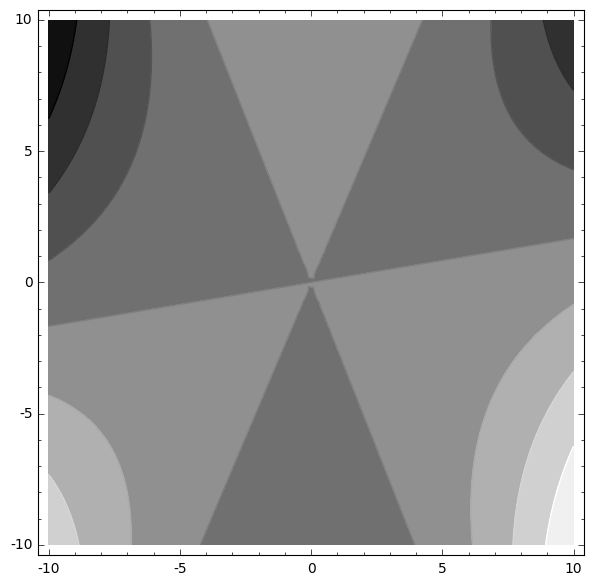
\includegraphics[width=5cm]{sage-algebraic-curve-plot}
\end{center}
from which we can see that our curve is a union of three lines.
Similarly
\begin{sageblock}
x,y=var('x,y')
contour_plot(y^2-x*(x-1)*(x-2)==0, (x,-3,4), (y,-5,5))
\end{sageblock}
yields level sets like
\begin{center}
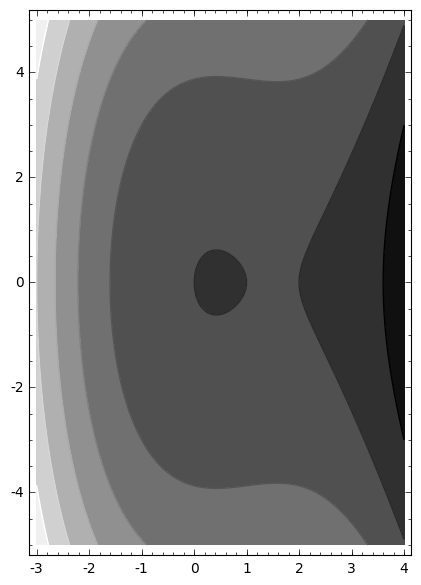
\includegraphics[width=5cm]{sage-algebraic-curve-plot-2}
\end{center}
and we can also plot the algebraic curve, without the other level sets, using
\begin{sageblock}
f(x,y) = y^2-x*(x-1)*(x-2)
implicit_plot(f, (-3, 4), (-5, 5))
\end{sageblock}
yielding
\begin{center}
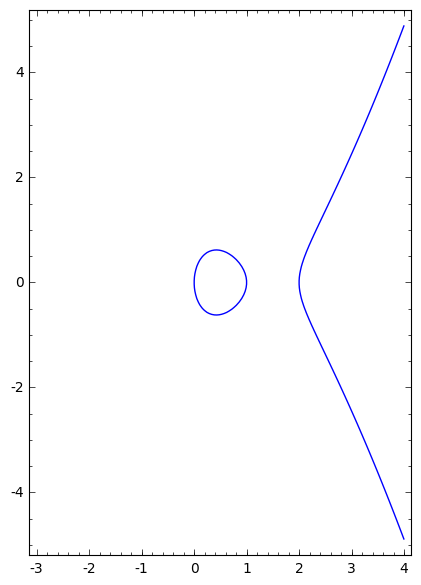
\includegraphics[width=5cm]{sage-algebraic-curve-plot-3}
\end{center}
Similarly, we can draw algebraic surfaces:
\begin{sageblock}
f(x,y,z) = y^2-x*(x-1)*(x-2)+z^4-1
implicit_plot3d(f, (-3, 4), (-5, 5), (-1,1))
\end{sageblock}
yielding
\begin{center}
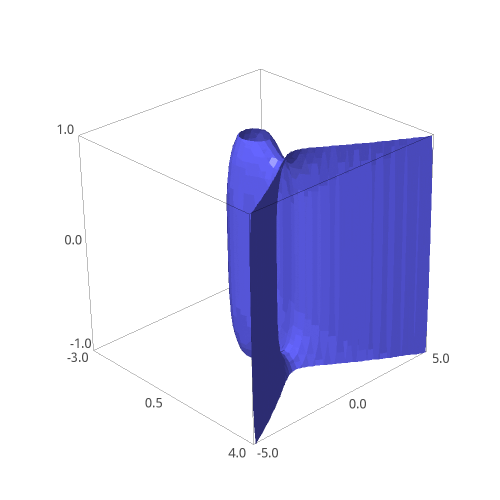
\includegraphics[width=5cm]{sage-algebraic-surface-plot}
\end{center}

\chapter{Where plane curves intersect}

\section{Vanishing polynomials}
\begin{example}
Over the finite field with two elements, \(t(t+1)\) vanishes for any value of \(t\) in that field.
\end{example}
\begin{example}
Over any finite field, the polynomial
\[
q(t) = \prod_c (t-c)
\]
(where the product is over all constants \(c\) in the field) vanishes for any value of the variable \(t\) in that field.
\end{example}
\begin{lemma}\label{lemma:infinite.field.zeroes}
Take a nonzero polynomial in several variables, over a field \(k\), that vanishes for all values of those variables.
Then the field \(k\) is finite and the polynomial is expressible as
\[
p(x)
=
\sum_{i=1}^n p_i(x) q\of{x_i}
\]
where \(x=\pr{x_1,x_2,\dots,x_n}\) and each \(p_i(x)\) is a polynomial and
\[
q(t)=\prod_c \pr{t-c}
\]
is our polynomial that vanishes for all values of \(t\) in \(k\).
In particular, \(p(x)\) has degree at least equal to the number of elements in the field in at least one of the variables.
\end{lemma}
\begin{proof}
In one variable, we can factor each root as in corollary~\vref{corollary:divide.poly}.
Suppose we have two variables \(x,y\) and a polynomial \(p(x,y)\).
Set \(y\) to zero, and find that by induction, the resulting polynomial \(p(x,0)\) is divisible as required by \(q(x)\), say \(p(x,0)=q(x)p_1(x)\).
So \(p(x,y)=q(x)p_1(x) + y h(x,y)\), say.
It is good enough to prove the result for \(y h(x,y)\) and add to \(q(x)p_1(x)\).
So we can assume that \(p(x,y)=y h(x,y)\).
Moreover, since \(p(x,y)\) vanishes for all \(x,y\) values in our field, \(h(x,y)\) vanishes for all \(x,y\) values in our field as long as \(y\ne 0\). 

Define a polynomial \(\delta(t)\) by
\[
\delta(t)=\prod_{c\ne 0}\pr{1-\frac{t}{c}},
\]
where the product is over all nonzero constant elements \(c\) in our field.
Check that \(\delta(0)=1\) while \(\delta(b)=0\) for any nonzero element \(b\) of our field.
Therefore
\[
h(x,y)-\delta(y)h(x,0)
\]
vanishes for all values of \(x,y\) in our field.
By induction on degree, we can write 
\[
h(x,y)-\delta(y)h(x,0)=h_1(x,y)q(x)+h_2(x,y)q(y).
\]
Plugging back into \(p(x,y)\) gives the result.
\end{proof}

\section{Linear factors}
A \emph{linear function}\define{linear!function} is a polynomial of the form
\[
f\of{x_1,x_2,\dots,x_n} = a_1 x_1 + a_2 x_2 + \dots + a_n x_n.
\]
If not all of the coefficients \(a_1, a_2, \dots, a_n\) are zero, the set of points \(x=\pr{x_1,x_2,\dots,x_n}\) at which \(f(x)=0\) is called a \emph{linear hyperplane}.\define{linear!hyperplane}\define{hyperplane!linear}
\begin{lemma}\label{lemma:linear.factor}
Suppose that in variables \(x=\pr{x_1,x_2,\dots,x_n}\)
\begin{enumerate}
  \item \(p(x)\) is a polynomial and
  \item \(f(x)\) is a nonzero linear function and
  \item \(p(x)=0\) at every point \(x\) where \(f(x)=0\) and
  \item the field we are working over contains more elements than the degree of \(p(x)\) in any variable.
\end{enumerate}
Then \(f(x)\) divides \(p(x)\), i.e. there is a polynomial \(q(x)\) so that \(p(x)=q(x)f(x)\).
\end{lemma}
\begin{proof}
By a linear change of variables, we can arrange that \(f(x)=x_1\).
Expand \(p(x)\) in powers of \(x_1\).
If there is a ``constant term'', i.e. a monomial in \(x_2, x_3, \dots, x_n\), then setting \(x_1=0\) we will still have some nonzero polynomial in the variables \(x_2, x_3, \dots, x_n\).
But this polynomial vanishes for all values of these variables, so is zero by lemma~\vref{lemma:infinite.field.zeroes}.
\end{proof}

\section{Resultants in many variables}
\pgfplotsset{width=5cm}%
\begin{lemma}\label{lemma:resultant.over.rings}
Take two polynomials \(b(x), c(x)\) in a variable \(x\), with coefficients in a commutative ring \(S\), of degrees \(m, n\).
Then the resultant\SubIndex{resultant} \(r=\resultant{b}{c}\) is expressible as \(r=u(x)b(x)+v(x)c(x)\) where \(u(x)\) and \(v(x)\) are polynomials, with coefficients in the same commutative ring \(S\), of degrees \(n-1, m-1\).
\end{lemma}
The proof is identical to the proof of lemma~\vref{lemma:resultant.over.integers}.

Take two polynomials \(b(x,y)\) and \(c(x,y)\) and let \(r(x)\) be the resultant of \(b(x,y), c(x,y)\) in the \(y\) variable, so thinking of \(b\) and \(c\) as polynomials in \(y\), with coefficients being polynomials in \(x\).
So \(r(x)\) is a polynomial in \(x\).
\begin{example}
If \(b(x,y)=y+x\), \(c(x,y)=y\), then \(r(x)=x\) vanishes just at the value \(x=0\) where there is a common factor: \(y\).
\begin{center}
\inputinexample{nondegenerate-resultant}
\end{center}
\end{example}
\begin{example}
Let \(b(x,y)\defeq xy^2+y\), \(c(x,y)\defeq xy^2+y+1\).
\begin{center}
\inputinexample{degenerate-resultant-2c}
\end{center}
Look at the picture at \(x=0\) and near \(x=0\): because the polynomials drop degrees, the number of roots of \(b(0,y)\) on the vertical line \(x=0\) is smaller than the number of roots of \(b(a,y)\) on the vertical line \(x=a\) for constants \(x=a\) near \(0\).
We can see roots ``flying away'' to infinity on those lines.
\begin{center}
\inputinexample{degenerate-resultant-2b}
\end{center}
Finding the determinant of the associated \(4 \times 4\) matrix tells us that \(r(x)=x^2\), which vanishes just at the value \(x=0\) where \(b(0,y)=y\) and \(c(0,y)=y+1\) drop in degrees, \emph{not} due to a common factor.
\begin{center}
\inputinexample{degenerate-resultant-2}
\end{center}
The resultant of \(y\) and \(y+1\) is \emph{not} \(r(0)\) since the degrees drop, so we would compute resultant of \(y\) and \(y+1\) using a \(2 \times 2\) matrix, and find resultant \(-1\).
\end{example}
\begin{example}
If \(b(x,y)=xy^2+y\) and \(c(x,y)=2xy^2+y+1\) then \(r(x)=x(x+1)\) vanishes at \(x=0\) and \(x=-1\).
At \(x=0\), \(b(0,y)=y, c(0,y)=y+1\) have no common factor, but drop degrees.
At \(x=-1\), \(b(-1,y)=-y(y-1)\), \(c(-1,y)=-2(y-1)(y-1/2)\) have a common factor, but they don't drop degrees. 
\begin{center}
\inputinexample{degenerate-resultant}
\end{center}
\end{example}
\begin{example}
If \(b(x,y)=x^2+y^2-1\) and \(c(x,y)=(x-1)^2+y^2-1\) then \(r(x)=(2x-1)^2\) vanishes at \(x=1/2\), where there are \emph{two} different intersection points, a double common factor:
\[
b(1/2,y)=c(1/2,y)=\pr{y-\frac{\sqrt{3}}{2}}\pr{y+\frac{\sqrt{3}}{2}}.
\]
\begin{center}
\inputinexample{degenerate-resultant-4}
\end{center}
\end{example}
\begin{lemma}\label{lemma:linear.normalization}
Suppose that \(k\) is a field and 
\[
x=\pr{x_1,x_2,\dots,x_n}
\]
are variables and \(y\) is a variable.
Take \(b(x,y)\) and \(c(x,y)\) two nonconstant polynomials in \(k[x,y]\).
Then in some finite degree extension of \(k\) there are constants 
\[
\lambda=\pr{\lambda_1, \lambda_2, \dots, \lambda_n}
\]
so that (writing \(\lambda y\) for \(\sum \lambda_i y_i\)) in the expressions \(b\of{x+\lambda y, y}, c\of{x+\lambda y,y}\), the coefficients of highest order in \(y\) are both nonzero constants.
\end{lemma}
\begin{example}
Return to our earlier example of \(b(x,y)=xy^2+y\) and \(c(x,y)=2xy^2+y+1\) and let
\begin{align*}
B(x,y) \defeq b(x+\lambda y,y) &= \lambda y^3 + xy^2 + y, \\
C(x,y) \defeq c(x+\lambda y,y) &= 2\lambda y^3 + 2xy^2 + y + 1.
\end{align*}
For any nonzero constant \(\lambda \ne 0\), the resultant of \(B(x,y), C(x,y)\) is 
\[
r(x)=
\det
\begin{pmatrix}
0 & 0 & 0 & 1 & 0 & 0 \\
1 & 0 & 0 & 1 & 1 & 0 \\
x & 1 & 0 & 2x & 1 & 1 \\
l & x & 1 & 2\lambda & 2 \, x & 1 \\
0 & l & x & 0 & 2\lambda & 2 \, x \\
0 & 0 & l & 0 & 0 & 2\lambda
\end{pmatrix}=-\lambda^2\pr{\lambda+1+x}.
\]
So the resultant now vanishes just when \(x=-(\lambda+1)\), which is precisely when \(B(x,y), C(x,y)\) have a common factor of \(y-1\).
With a small value of \(\lambda \ne 0\), the picture changes very slightly: we change \(x,y\) to \(x+\lambda y,y\), a linear transformation which leaves the \(x\)-axis alone, but tilts the \(y\)-axis to the left.
Crucially, we tilt the asymptotic line at which the two curves approached one another (where \(b(x,y)\) and \(c(x,y)\) dropped degrees), but with essentially no effect on the intersection point:
\begin{center}
\inputinexample{degenerate-resultant-3}
\end{center}
\end{example}
\begin{example}
If \(b(x,y)=x^2+y^2-1\) and \(c(x,y)=(x-1)^2+y^2-1\), then \(r(x)=(2x-1)^2\) vanishes at \(x=1/2\), where there are \emph{two} different intersection points.
\begin{center}
\inputinexample{degenerate-resultant-4}
\end{center}
If instead we pick any nonzero constant \(\lambda\) and let \(B(x,y)\defeq (x+\lambda y)^2+y^2-1\) and \(C(x,y)\defeq (x+\lambda y - 1)^2+y^2-1\) then the resultant
\[
r(x)=4
\pr{\lambda^2 + 1}
\pr{
	x
	-
	\frac{1+\lambda\sqrt{3}}{2}
}
\pr{
	x
	-
	\frac{1-\lambda\sqrt{3}}{2}
}
\]
vanishes at two distinct values of \(x\) corresponding to the two distinct roots.
In the picture, the two roots now lie on different vertical lines (different values of \(x\)).
\begin{center}
\inputinexample{nondegenerate-resultant-2}
\end{center}
\end{example}
\begin{proof}
Write \(b\) as a sum of homogeneous polynomials of degrees \(0, 1, 2, \dots, d\), say 
\[
b=b_0+b_1+\dots+b_d.
\]
It is enough to prove the result for \(b_d\), so assume that \(b\) is homogeneous of degree \(d\).
The expression
\[
b\of{x,1}
\]
is a nonzero polynomial over an infinite field, so doesn't vanish everywhere by lemma~\vref{lemma:infinite.field.zeroes}.
Pick \(\lambda\) to be a value of \(x\) for which \(b\of{\lambda,1}\ne 0\).
Then
\[
b(x+\lambda y,y)=yb(x,1)+\dots+y^d b(\lambda,1).
\]
Similarly for two polynomials \(b(x,y), c(x,y)\), or for any finite set of polynomials.
\end{proof}

\begin{corollary}\label{corollary:resultant.effective}
Take one variable \(y\) and several variables \(x=\pr{x_1,x_2,\dots,x_n}\) and two polynomials \(b(x,y)\) and \(c(x,y)\) over a field.
Let \(r(x)\) be the resultant of \(b(x,y), c(x,y)\) in the \(y\) variable.
For any constant \(a\) in our field, if \(b(a,y)\) and \(c(a,y)\) have a common root in some algebraic extension of our field then \(r(a)=0\).

If the coefficient of highest order in \(y\) of both \(b(x,y)\) and \(c(x,y)\) is constant in \(x\) (for example, perhaps after the normalization described in lemma~\vref{lemma:linear.normalization}) then \(r(a)=0\) at some value \(x=a\) in our field just exactly when \(b(a,y)\) and \(c(a,y)\) have a common factor.
Moreover \(r(x)\) is then the zero polynomial just when \(b(x,y)\) and \(c(x,y)\) have a common factor which is a polynomial in \(x,y\) of positive degree in \(y\).
\end{corollary}
\begin{proof}
If, at some value \(x=a\), both the degrees of \(b(x,y)\) and \(c(x,y)\) don't drop, then the resultant in \(y\) is expressed by the same expression whether we set \(x=a\) to a constant value or leave \(x\) as an abstract variable, compute resultant, and then set \(x=a\).

Work over the ring of polynomials in \(y\), with coefficients rational in \(x\).
The resultant in \(y\) being zero as a function of \(x\) forces a common factor in that ring, i.e.
\begin{align*}
b(x,y)&=d(x,y)B(x,y), \\
c(x,y)&=d(x,y)C(x,y),
\end{align*}
where \(d(x,y), B(x,y)\) and \(C(x,y)\) are rational in \(x\) and polynomial in \(y\) and \(d(x,y)\) has positive degree in \(y\).
In particular, \(c(x,y)\) factorises over that ring.
By the Gauss lemma (proposition~\vref{proposition:Gauss.lemma}), \(c(x,y)\) factorises over the polynomials in \(x,y\).
But \(c(x,y)\) is irreducible, so one factor is constant, and it isn't \(d(x,y)\), so it must be \(C(x,y)\), so we rescale by a nonzero constant to get \(d(x,y)=c(x,y)\), i.e. \(c(x,y)\) divides \(b(x,y)\).
\end{proof}

\begin{corollary}\label{corollary:Null}
Given a finite collection of polynomial functions over a field \(k\), for \(x=\pr{x_1,x_2,\dots,x_n}\), either
\begin{enumerate}
\item
in some finite extension of \(k\), there is at least one point on which all polynomials in the collection vanish or
\item
in some finite extension of \(k\), every polynomial lies in the ideal generated by this collection.
\end{enumerate}
\end{corollary}
\begin{proof}
Suppose we just have two polynomials \(p_1(x)\) and \(p_2(x)\) in our collection.
As above, after perhaps a finite extension, and a linear change of variables, we compute a resultant to find the values of one fewer of the variables on which there are simultaneous zeroes.
The result follows by induction.
Suppose instead that there are finitely many polynomials in our collection.
We repeatedly replace pairs by such resultants, to eventually reduce the number of variables, and apply induction on the variables.
In the end, when we have only one variable: all resultants are constants, and if they are not all zero, then there are no simultaneous solutions.
Suppose that there is a nonzero resultant in among these.
Rescale to get its value to be 1.
That nonzero resultant is expressed as a linear combination as in lemma~\vref{lemma:resultant.over.rings}.
By induction we construct polynomials \(q_j(x)\) so that 
\[
1 = q_1(x)p_1(x) + q_2 p_2(x) + \dots + q_s(x) p_s(x).
\]
So \(1\) lies in the ideal generated by these \(p_1(x), p_2(x), \dots, p_s(x)\).
But then any polynomial \(f(x)\) has the form \(f(x)=f(x) \cdot 1\), so also lies in that ideal.
\end{proof}



\chapter{Quotient rings}\label{chapter:quotient.rings}

Recall once again that all of our rings are assumed to be commutative rings with identity.
Suppose that \(R\) is a ring and that \(I\) is an ideal.
For any element \(r \in R\), then \emph{translate} of \(I\) by \(r\), denoted \(r+I\), is the set of all elements \(r+i\) for any \(i \in I\).
\begin{example}
If \(R=\Z{}\) and \(I=12\Z{}\) is the multiples of \(12\), then \(7+I\) is the set of integers which are 7 larger than a multiple of \(12\), i.e. the set of all numbers 
\[
\dots,7-12,7,7+12,7+2 \cdot 12, 7+3 \cdot 12, \dots
\]
which simplifies to
\[
\dots,-5,7,19,31,53, \dots
\]
But this is the same translate as \(-5+I\), since \(-15+12=7\) so \(-5+I\) is
the set of all numbers
\[
\dots,-5-12,-5,-5+12,-5+2 \cdot 12, -5+3 \cdot 12, \dots
\]
which is just 
\[
\dots,-15,-5,7,19,31,53, \dots
\]
the same sequence.
\end{example}
\begin{example}
Working again inside \(\Z{}\), \(2+2\Z{}=2\Z{}\) is the set of even integers.
\end{example}
\begin{example}
If \(R=\Q{}[x]\) and \(I=(x)\), then \(\frac{1}{2}+I\) is the set of all polynomials of the form
\[
\frac{1}{2}+xp(x)
\]
for any polynomial \(p(x)\).
\end{example}
\begin{example}
If \(i \in I\) then \(i+I=I\).
\end{example}
We add two translates by
\[
\pr{r_1+I}+\pr{r_2+I}\defeq \pr{r_1+r_2}+I,
\]
and multiply by
\[
\pr{r1+I}\pr{r_2+I}=\pr{r_1r_2}+I.
\]
\begin{lemma}\label{lemma:translates}
For any ideal \(I\) in any ring \(R\), two translates \(a+I\) and \(b+I\) are equal just when \(a\) and \(b\) differ by an element of \(I\).
\end{lemma}
\begin{proof}
We suppose that \(a+I=b+I\).
Clearly \(a\) belongs to \(a+I\), because \(0\) belongs to \(I\).
Therefore \(a\) belongs to \(a+I=b+I\), i.e. \(a=b+i\) for some \(i\) from \(I\).
\end{proof}

\begin{lemma}
The addition and multiplication operations on translates are well defined, i.e. if we find two different ways to write a translate as \(r+I\), the results of adding and multiplying translates don't depend on which choice we make of how to write them.
\end{lemma}
\begin{proof}
You write your translates as \(a_1+I\) and \(a_2+I\), and I write mine as \(b_1+I\) and \(sb_2+I\), but we suppose that they are the same subsets of the same ring: \(a_1+I=b_1+I\) and \(a_2+I=b_2+I\).
By lemma~\vref{lemma:translates}, \(a_1=b_1+i_i\) and \(a_2=b_2+i_2\) for some elements \(i_1, i_2\) of \(I\). 
So then
\begin{align*}
a_1+a_2+I
&=
b_1+i_1+b_2+i_2+I,
\\
&=
b_1+b_2+\pr{i_1+i_2}+I,
\\
&=
b_1+b_2+I.
\end{align*}
The same for multiplication.
\end{proof}

If \(I\) is an ideal in a commutative ring \(R\), the \emph{quotient ring}\define{quotient ring} \(R/I\)\Notation{R/I}{R/I}{quotient of a ring by an ideal} is the set of all translates of \(I\), with addition and multiplication of translates as above.
The reader can easily prove:
\begin{lemma}
For any ideal \(I\) in any commutative ring \(R\), \(R/I\) is a commutative ring.
If \(R\) has an identity element then \(R/I\) has an identity element.
\end{lemma}

\begin{example}
If \(R\defeq\Z{}\) and \(I\defeq m\Z{}\) for some integer \(m\) then \(R/I=\Zmod{m}\) is the usual ring of remainders modulo \(m\).
\end{example}
\begin{example}
If \(p(x,y)\) is an irreducible nonconstant polynomial over a field \(k\) and \(I=(p(x,y))=p(x,y)k[x]\) is the associated ideal, then \(k[x,y]/I=k[X]\) is the  ring of regular functions on the algebraic plane curve \(X=(p(x,y)=0)\).
\end{example}

\begin{lemma}
A ideal \(I\) in a ring \(R\) with identity is all of \(R\) just when \(1\) is in \(I\).
\end{lemma}
\begin{proof}
If \(1\) lies in \(I\), then any \(r\) in \(R\) is \(r=r1\) so lies in \(I\), so \(I=R\).
\end{proof}

An ideal \(I\) in a ring \(R\) is \emph{prime}\define{prime ideal}\define{ideal!prime} if \(I\) is not all of \(R\) and, for any two elements \(a, b\) of \(R\), if \(ab\) is in \(I\) then either \(a\) or \(b\) lies in \(I\).

\begin{example}
The ideal \(p\Z{}\) in \(\Z{}\) generated by any prime number is prime.
\end{example}
\begin{example}
The ring \(R\) is \emph{not} prime in \(R\), because the definition explicitly excludes it.
\end{example}
\begin{example}
Inside \(R\defeq \Z{}[x]\), the ideal \((x)\) is prime, because in order to have a factor of \(x\) sitting in a product, it must lie in one of the factors.
\end{example}
\begin{example}
Inside \(R\defeq \Z{}[x]\), the ideal \((2x)\) is \emph{not} prime, because \(a=2\) and \(b=x\) multiply to a multiple of \(2x\), but neither factor is a multiple of \(2x\).
\end{example}
\begin{example}
If \(p(x)\) is an irreducible polynomial, then \((p(x))\) is a prime ideal.
\end{example}
\begin{example}
The regular functions on an algebraic curve \(p(x,y)=0\) over a field \(k\) constitute the ring \(R/I\) where \(R=k[x,y]\) and \(I=(p(x,y))\).
The curve is irreducible just when the ideal is prime.
\end{example}
\begin{example}
Take a field \(k\).
In the quotient ring \(R=k[x,y,z]/(z^2-xy)\), the ideal \((z)\) contains \(z^2=xy\), but does not contain \(x\) or \(y\), so is not prime.
\end{example}

\begin{lemma}
An ideal \(I\) in a commutative ring with identity \(R\) is prime just when \(R/I\) has no zero divisors, i.e. no nonzero elements \(\alpha, \beta\) can have \(\alpha\beta=0\).
\end{lemma}
\begin{proof}
Write \(\alpha\) and \(\beta\) as translates \(\alpha=a+I\) and \(\beta=b+I\).
Then \(\alpha\beta=0\) just when \(ab+I=I\), i.e. just when \(ab\) lies in \(I\).
On the other hand, \(\alpha=0\) just when \(a+I=I\), just when \(a\) is in \(I\).
\end{proof}

A ideal \(I\) in a ring \(R\) is \emph{maximal}\define{ideal!maximal}\define{maximal ideal} if \(I\) is not all of \(R\) but any ideal \(J\) which contains \(I\) is either equal to \(I\) or equal to \(R\) (nothing fits in between).

\begin{lemma}
If \(I\) is an ideal in a commutative ring \(R\) with identity, then \(I\) is a maximal ideal just when \(R/I\) is a field.
\end{lemma}
\begin{proof}
Suppose that \(I\) is a maximal ideal.
Take any element \(\alpha \ne 0\) of \(R/I\) and write it as a translate \(\alpha=a+I\).
Since \(\alpha \ne 0\), \(a\) is not in \(I\).
We know that \((a)+I=R\), since \(I\) is maximal.
But then \(1\) lies in \((a)+I\), so \(1=ab+i\) for some \(b\) in \(R\) and \(i\) in \(I\).
Expand out to see that 
\[
\frac{1}{\alpha}=b+I.
\]
So nonzero elements of \(R/I\) have reciprocals.

Suppose instead that \(R/I\) is a field.
Take an element \(a\) in \(R\) not in \(I\).
Then \(a+I\) has a reciprocal, say \(b+I\).
But then \(ab+I=1+I\), so that \(ab=1+i\) for some \(i\) in \(I\).
So \((a)+I\) contains \((ab)+I=(1)=R\). 
\end{proof}

\begin{example}
If \(p\) is a prime number, then \(I \defeq p\Z{}\) is maximal in \(R\defeq \Z{}\), because any other ideal \(J\) containing \(I\) and containing some other  integer, say \(n\), not a multiple of \(p\), must contain the greatest common divisor of \(n\) and \(p\), which is \(1\) since \(p\) is prime.
We recover the fact that \(\Zmod{p}\) is a field.
\end{example}
\begin{example}
The ideals in \(R\defeq \Zmod{4}\) are \((0),(1)=\Zmod{4}\) and \((2)\cong \Zmod{2}\), and the last of these is maximal.
\end{example}
\begin{example}
Take a field \(k\) and let \(R\defeq k[x]\).
Every ideal \(I\) in \(R\) has the form \(I=(p(x))\), because each ideal is generated by the greatest common divisor of its elements.
We have seen that \(R/I\) is prime just when \(p(x)\) is irreducible.
To further have \(R/I\) a field, we need \(I=(p(x))\) to be maximal.
Take some polynomial \(q(x)\) not belonging to \(I\), so not divisible by \(p(x)\).
Since \(p(x)\) is irreducible, \(p(x)\) has no factors, so \(\gcd{p(x),q(x)}=1\) in \(k[x]\), so that the ideal generated by \(p(x),q(x)\) is all of \(R\).
Therefore \(I=(p(x))\) is maximal, and the quotient \(R/I=k[x]/(p(x))\) is a field.
\end{example}
\begin{example}
If \(k\) is an algebraically closed field and \(R\defeq k[x]\) then every irreducible polynomial is linear, so every maximal ideal in \(R\) is \(I=(x-c)\) for some constant \(c\).
\end{example}


\begin{problem}{quotient.rings:ideals.in.Zm}
For any positive integer \(m \ge 2\), what are the prime ideals in \(\Zmod{m}\), and what are the maximal ideals?
\end{problem}

\section{Sage}

We take the ring \(R=\Q{}[x,y]\) and then quotient out by the ideal \(I=(x^2y,xy^3)\) to produce the ring \(S=R/I\).
The generators \(x,y\) in \(R\) give rise to elements \(x+I,y+I\) in \(S\), which are renamed to \(a,b\) for notational convenience.
\begin{sageblock}
R.<x,y> = PolynomialRing(QQ)
I = R.ideal([x^2*y,x*y^3])
S.<a,b> = R.quotient_ring(I)
(a+b)^4
\end{sageblock}
which yields \(\sage{(a+b)^4}\).

We can define \(R=\Q{}[x,y]\), \(I=(y^2)\), \(S=R/I\) where we label \(x+I, y+I\) as \(a,b\), \(T=\Q{}[z]\) and define a morphism \(\phi \colon S \to T\) by  \(\phi(a)=z^3, \phi(b)=0\):
\begin{sageblock}
R.<x,y> = PolynomialRing(QQ)
I = R.ideal([y^2])
S.<a,b> = R.quotient_ring(I)
T.<z> = PolynomialRing(QQ)
phi = S.hom([z^3, 0],T)
phi(a^2+b^2)
\end{sageblock}
yielding \(\sage{phi(a^2+b^2)}\).


\section{Automorphisms of splitting fields}
\begin{theorem}\label{theorem:splitting.fields.exist}
Suppose that \(k\) is a field and \(p(x)\) is a nonconstant polynomial over \(k\), say of degree \(n\).
Any two splitting fields for \(p(x)\) over \(k\) are isomorphic by an isomorphism which is the identity on \(k\).
\end{theorem}
\begin{proof}
We already know that splitting fields exist, by adding roots to irreducible factors of \(p(x)\).
Each time we add a root, the dimension of the extension field over \(k\) is the degree of the irreducible factor.
We then split off at least one linear factor in the extension field, and repeat.
So at most \(n!\) degree in total.

Given any splitting field \(K\) for an irreducible polynomial \(p(x)\), pick any root \(\alpha \in K\) of \(p(x)\) and map
\[
f(x) \in k[x] \mapsto f(\alpha) \in K,
\]
to see that \(K \cong k[x]/I\).
Hence \(K\) is uniquely determined up to isomorphism.

Suppose instead that \(p(x)\) is reducible, and that \(K,L\) are splitting fields of \(p(x)\).
Pick an irreducible factor \(q(x)\) of \(p(x)\).
Then the subfields of \(K,L\) generated by adding a root of \(q(x)\) to \(k\) are isomorphic, since \(q(x)\) is irreducible, so we can assume that these subfields are the same field.
We need only split \(p(x)\) over that field, or quotient out all copies of \(q(x)\) from \(p(x)\) and split the result.
Apply induction on the degree of \(p(x)\).
\end{proof}
\begin{example}
Adding a root to \(x^2+1\) over \(\R{}\) yields the splitting field \(\C{}\).
\end{example}
\begin{theorem}\label{theorem:irreducible.orbit}
Suppose that \(K\) is a splitting field of an irreducible polynomial \(p(x)\) over a field \(k\).
If \(\alpha,\beta \in K\) are roots of \(p(x)\) then the Galois group of \(K\) over \(k\) has an element which takes \(\alpha\) to \(\beta\).
In particular, \(K\) is a Galois extension of \(k\).
\end{theorem}
\begin{proof}
As in the proof of theorem~\vref{theorem:splitting.fields.exist}, there is a field isomorphism \(k[x]/I \to K\) taking \(x \mapsto \alpha\), and another field isomorphism \(k[x]/I \to K\) taking \(x \mapsto \beta\).
\end{proof}

\section{Transcendental numbers}
A number \(\alpha \in \C{}\) is \emph{algebraic} if it is the solution of a polynomial equation \(p(\alpha)=0\) where \(p(x)\) is a nonzero polynomial with rational coefficients.
A number which is not algebraic is called \emph{transcendental}.
More generally, given a field extension \(K\) of a field \(k\), an element \(\alpha \in K\) is \emph{algebraic} over \(k\) if it is a root of a nonzero polynomial \(p(x)\) with coefficients in \(k\).
\begin{theorem}
For any field extension \(K\) of a field \(k\), an element \(\alpha \in K\) is transcendental if and only if the field 
\[
k(\alpha) = \Set{\frac{p(\alpha)}{q(\alpha)}|\frac{p(x)}{q(x)} \in k(x) \text{ and } q(\alpha) \ne 0}
\]
is isomorphic to \(k(x)\).
\end{theorem}
\begin{proof}
If \(\alpha\) is transcendental, then the map
\[
f \colon \frac{p(x)}{q(x)} \in k(x) \mapsto \frac{p(\alpha)}{q(\alpha)} \in k(\alpha)
\]
is clearly well defined, onto, and preserves all arithmetic operations.
To show that \(f\) is 1-1 is the same as showing that \(f\) has trivial kernel.
Suppose that \(p(x)/q(x)\) lies in the kernel of \(f\).
Then \(p(\alpha)=0\), so \(p(x)=0\), so \(p(x)/q(x)=0\).
So the kernel is trivial, and so \(f\) is a bijection preserving all arithmetic operations, so \(f\) is an isomorphism of fields.

On the other hand, take a element \(\alpha\) in \(K\) and suppose that there is some isomorphism of fields
\[
g \colon k(x) \to k(\alpha).
\]
Let \(\beta\defeq g(x)\).
Because \(g\) is a field isomorphism, all arithmetic operations carried out on \(x\) must then be matched up with arithmetic operations carried out on \(\beta\), so
\[
g\left(\frac{p(x)}{q(x)}\right)=\frac{p(\beta)}{q(\beta)}.
\]
Because \(g\) is an isomorphism, some element must map to \(\alpha\), say
\[
g\left(\frac{p_0(x)}{q_0(x)}\right)=\alpha.
\]
So
\[
\frac{p_0(\beta)}{q_0(\beta)}=\alpha.
\]
So \(k(\beta)=k(\alpha)\).
Any algebraic relation on \(\alpha\) clearly gives one on \(\beta\) and vice versa.
Therefore \(\alpha\) is algebraic if and only if \(\beta\) is.
Suppose that \(\beta\) is algebraic.
Then \(q(\beta)=0\) for some polynomial \(q(x)\), and then \(g\) is not defined on \(1/q(x)\), a contradiction.
\end{proof}

\section{Finite fields}
We are going to make a complete list of all finite fields.
Pick a prime number \(p\) and work over the field \(k=\Zmod{p}\).
For any integer \(n>0\), the polynomial \(x^{p^n}-x\) has two obvious linear factors: \(x\) and \(x-1\), and then factors as
\[
x^{p^n}-x
=
x(x-1)(x^{-2+p^n} + x^{-3+p^n} + \dots + x + 1).
\]
\begin{lemma}\label{lemma:splits.neatly}
For any prime \(p\), over any extension field \(K\) of the field \(k=\Zmod{p}\), the polynomial 
\[
x^{p^n}-x
\]
has no multiple roots.
\end{lemma}
\begin{proof}
Let \(c(x)\defeq x^{p^n}-x\).
As above, write \(x(x-1)b(x)=c(x)\).
Note that \(b(0)=1\ne 0\) and \(b(1)=p^n-1=-1\ne 0\).
If, in some field \(K\), we can factor out a multiple root from \(b(x)\), that multiple root is not at \(x=0\) or \(x=1\), so we can factor out the same multiple root from \(c(x)=x(x-1)b(x)\).
Take the derivative of \(c(x)\):
\[
c'(x)= \frac{d}{dx} \pr{x^{p^n}-x}=p^n x^{-1+p^n} - 1= -1,
\]
since \(p=0\) in \(k\).
But then \(c'(x)\) has no roots in any field extension \(K\) of \(k\), so \(c(x)\) has no multiple roots over \(K\), so \(b(x)\) has no multiple roots over \(K\).
\end{proof}
\begin{lemma}
For any finite field \(k\) of characteristic \(p\), the \emph{Frobenius morphism}\define{Frobenius morphism}\define{morphism!Frobenius} \(f(x)=x^p\) is an automorphism of fields \(f \colon k \to k\), i.e. is a bijection preserving addition, subtraction, multiplication and division, taking \(0 \mapsto 0\) and \(1 \mapsto 1\).
\end{lemma}
\begin{proof}
Clearly \(0^p=0\) and \(1^p=1\).
For any \(b,c \in k\), clearly \((bc)^p)=b^pc^p\).
The binomial theorem gives
\[
(b+c)^p = b^p + p b^{p-1} c + \frac{p(p-1)}{2} b^{p-2} c^2 + \dots + \frac{p!}{j!(p-j)!} b^{p-j} c^j + \dots + c.
\]
Every term except \(b\) and \(c\) has a factor of \(p\) in it, and \(p=0\) in \(k\), so
\[
(b+c)^p=b^p+c^p.
\]
The same for \((b-c)^p=b^p-c^p\). 
If \(f(b)=0\), then \(b^p=0\) so \(b \cdot b^{p-1}=0\) so \(b=0\) or \(b^{p-1}=0\), and by induction, we find that \(b=0\).
If \(f(b)=f(c)\) then \(f(b-c)=0\) so \(b-c=0\) so \(b=c\), i.e. \(f\) is 1-1.
But then, since \(k\) is finite, \(f\) is a bijection.
\end{proof}
\begin{theorem}
For any prime \(p\), the splitting field \(K\) of the polynomial
\[
c(x) = x^{p^n}-x
\]
over the field \(k=\Zmod{p}\) has \(p^n\) elements, every one of which is a root of \(c(x)\).
Every finite field \(K\) is obtained uniquely as the splitting field of \(c(x)\) for some prime number \(p\) and integer \(n \ge 1\), and so is uniquely determined up to isomorphism by its number of elements \(p^n\).
\end{theorem}
\begin{proof}
There are \(p^n\) roots of \(c(x)=x^{p^n}-x\) over its splitting field \(K\), since \(b(x)\) splits into linear factors, and, by lemma~\vref{lemma:splits.neatly} each linear factor gives a distinct root.
Given any roots \(\alpha,\beta\) of \(c(x)\), 
\[
\alpha^{p^n}=\alpha, \ \beta^{p^n}=\beta.
\]
Apply the Frobenius morphism:
\[
(\alpha+\beta)^{p^n} = \alpha^{p^n}+\beta^{p^n} = \alpha + \beta,
\]
so \(c(\alpha+\beta)=0\).
Similarly 
\[
(\alpha\beta)^{p^n}=\alpha^{p^n}\beta^{p^n}=\alpha\beta,
\]
so \(c(\alpha\beta)=0\).
Hence the roots of \(c(x)\) form a field, over which \(c(x)\) splits, and so \(b(x)\) splits.
So every element of \(K\) is a root of \(c(x)\), and so \(K\) is a splitting field of \(c(x)\) with \(p^n\) elements.
By the existence and uniqueness of splitting fields in theorem~\vref{theorem:splitting.fields.exist}, \(K\) is the unique splitting field of \(c(x)\).

Take any finite field \(L\), say of characteristic \(p\).
We map \(0,1,2,\dots,p-1\) in \(k=\Zmod{p}\) to \(0,1,2,\dots,p-1\) in \(L\), a morphism of fields.
Hence \(L\) is a vector space over \(k\), of finite dimension, say \(n\), and so has \(p^n\) elements.
The Frobenius morphism is an invertible \(k\)-linear map of \(L\), generating a subgroup of the group of invertible \(k\)-linear maps \(L \to L\).
This subgroup is finite, since there are only finitely many elements of \(L\), so finitely many permutations of those elements.
This subgroup is generated by a single element, so is cyclic.
By theorem~\vref{theorem:cyclic.groups}, this subgroup is isomorphic to \(\Zmod{\ell}\), for some integer \(\ell > 0\), so every element of \(L\) satisfies some equation \(x^{p^{\ell}}=x\).
\end{proof}
For any finite field \(k\), say with \(p^n\) elements, we can associate to any \(\alpha,\beta \in k\) the quadratic equation \((x-\alpha)(x-\beta)=0\) which has roots \(\alpha,\beta\).
On the other hand, given a quadratic equation \(x^2+bx+c=0\), we can ask whether it has roots.
Those with roots are given as \(x^2+bx+c=(x-\alpha)(x-\beta)\) for some \(\alpha,\beta\), unique up to swapping the order in which we write them down.
As there are \(p^n\) elements, there are 
\[
\frac{p^n(p^n+1)}{2}
\]
pairs \(\alpha,\beta\) of possible roots, up to swapping order.
But there are \(p^{2n}\) quadratic equations \(x^2+bx+c\): choose any \(b,c\) from \(k\).
So 
\[
p^{2n}-\frac{p^n(p^n+1)}{2}
=
\frac{p^n(p^n-1)}{2}
\]
quadratic equations over \(k\) have no solution in \(k\).

In particular, let \(k_1 \subset k_2 \subset k_3 \dots\) be finite fields or orders \(2,4,8\) and so on.
Each \(k_{n+1}\) is the splitting field of the polynomial \(z^2+z+\alpha\) over \(k_n\) where \(\alpha\) is any element of \(k_n\) not belonging to \(k_{n-1}\). 
In particular, we can see which quadratic equations have solutions in which fields of characteristic 2.
Note that we can't use the quadratic formula in fields of characteristic 2, because the quadratic formula has a 2 in it.

\begin{problem}{fields:double}
Prove by induction that if \(k\) is a finite field of characteristic 2, then every element \(\alpha\) of \(k\) is a square, i.e. \(\alpha=\beta^2\) for some \(\beta\).
\end{problem}
\begin{answer}{fields:double}
Let \(k_1 \subset k_2 \subset k_3 \dots\) be finite fields or orders \(2,4,8\) and so on.
Our result is clear if \(k=k_1=\Zmod{2}\).
By induction, suppose that our result is true for \(k_1, k_2, \dots, k_{n-1}\).
All of the elements \(\alpha\) of \(k_n\) that are not elements of \(k_{n-1}\) satisfy \(\alpha^2+\alpha+c=0\) for some \(c\) in \(k_{n-1}\), as we saw above.
By induction, \(c=b^2\) for some element \(b\) of \(k_{n-1}\).
So \(\alpha^2+\alpha+b^2=0\), i.e. \(\alpha^2+b^2=\alpha\).
Expand out \((\alpha+b)^2\) to find \((\alpha+b)^2=\alpha\).
\end{answer}

\section{Sage}
Lets get sage to construct the splitting field \(K\) of \(p(x)\defeq x^2+x+1\) over the field \(k=\Zmod{2}\).
Sage constructs splitting fields by first building a ring, which we will call \(R\), of polynomials over a field.
In our case, we build \(R=k[x]\).
Then we let \(K\) be the field generated by an element \(a\), which corresponds to the variable \(x\) in the polynomial ring \(R\).
\begin{sageblock}
R.<x> = PolynomialRing(GF(2))
K.<a> = (x^2 + x + 1).splitting_field()
\end{sageblock}
We can then make a list of some elements of \(K\), call it \(S\), and compute out addition and multiplication tables:
\begin{sageblock}
S=[0,1,a,a+1]
print("Addition table:")
for i in range(0,4):
    for j in range(0,4):
        print("({})+({})={}".format(S[i],S[j],S[i]+S[j]))
print("Multiplication table:")
for i in range(0,4):
    for j in range(0,4):
        print("({})*({})={}".format(S[i],S[j],S[i]*S[j]))
\end{sageblock}



\chapter{Field extensions and algebraic curves}

We can sometimes draw pictures of field extensions.
Take an algebraic curve \(C=(p(x,y)=0)\) in the plane, and look at its field of rational functions \(k(C)\), our favourite example of a field extension of a field \(k\).
\begin{center}
\pgfplotsset{compat=1.12,width=7cm}%
\documentclass{standalone}
\usepackage{tikz}
\usepackage{pgfplots}
\usepackage{xparse}
\pgfplotsset{compat=1.12,width=7cm}%
\colorlet{curveZero}{gray!75}
\colorlet{curveOne}{blue!60}
\colorlet{curveTwo}{brown!50!gray}
\colorlet{curveThree}{green!40!gray}
\colorlet{curveFour}{red!50!gray}
\NewDocumentCommand\DrawDotInPlot{O{}mmO{}}%
{%
\fill[gray!20,draw=gray] (axis cs:{#2},{#3}) circle (1.3pt) node[above,black,#4] {\(#1\)};%
}%
\NewDocumentCommand\DrawDot{O{}mmO{}}%
{%
\fill[gray!20,draw=gray] ({#2},{#3}) circle (1.3pt) node[above,black,#4] {\(#1\)};%
}%
\NewDocumentCommand\DrawNode{O{}m}%
{%
\fill[gray!20,draw=gray] (#2) circle (1.3pt) node[above,black] {\(#1\)};%
}%
\colorlet{axisColor}{gray!50}
\tikzstyle{shapeZero}=[fill=curveZero,opacity=.4]
\tikzstyle{shapeOne}=[fill=curveOne,opacity=.4]
\tikzstyle{shapeTwo}=[fill=curveTwo,opacity=.4]
\tikzstyle{shapeThree}=[fill=curveThree,opacity=.4]
\tikzstyle{groupElementLabel}=[minimum size=2.4em]
\tikzstyle{groupElement}=[minimum size=2.4em,shapeZero,draw=curveZero]
\tikzstyle{cosetOne}=[minimum size=2.4em,shapeOne,draw=curveOne]
\tikzstyle{cosetTwo}=[minimum size=2.4em,shapeTwo,draw=curveTwo]


\begin{document}
\begin{tikzpicture}
\begin{axis}[hide axis,xmin=-2,xmax=2,ymin=-2,ymax=2]
\newcommand{\RRR}{1.8}
\draw[axisColor] 
	({\RRR*cos(3.1415*0/10 r)},{\RRR*sin(3.1415*0/10 r)}) 
-- ({-\RRR*cos(3.1415*0/10 r)},{-\RRR*sin(3.1415*0/10 r)});
\draw[axisColor] 
	({\RRR*cos(3.1415*1/10 r)},{\RRR*sin(3.1415*1/10 r)}) 
-- ({-\RRR*cos(3.1415*1/10 r)},{-\RRR*sin(3.1415*1/10 r)});
\draw[axisColor] 
	({\RRR*cos(3.1415*2/10 r)},{\RRR*sin(3.1415*2/10 r)}) 
-- ({-\RRR*cos(3.1415*2/10 r)},{-\RRR*sin(3.1415*2/10 r)});
\draw[axisColor] 
	({\RRR*cos(3.1415*3/10 r)},{\RRR*sin(3.1415*3/10 r)}) 
-- ({-\RRR*cos(3.1415*3/10 r)},{-\RRR*sin(3.1415*3/10 r)});
\draw[axisColor] 
	({\RRR*cos(3.1415*4/10 r)},{\RRR*sin(3.1415*4/10 r)}) 
-- ({-\RRR*cos(3.1415*4/10 r)},{-\RRR*sin(3.1415*4/10 r)});
\draw[axisColor] 
	({\RRR*cos(3.1415*1/10 r)},{-\RRR*sin(3.1415*1/10 r)}) 
-- ({-\RRR*cos(3.1415*1/10 r)},{\RRR*sin(3.1415*1/10 r)});
\draw[axisColor] 
	({\RRR*cos(3.1415*2/10 r)},{-\RRR*sin(3.1415*2/10 r)}) 
-- ({-\RRR*cos(3.1415*2/10 r)},{\RRR*sin(3.1415*2/10 r)});
\draw[axisColor] 
	({\RRR*cos(3.1415*3/10 r)},{-\RRR*sin(3.1415*3/10 r)}) 
-- ({-\RRR*cos(3.1415*3/10 r)},{\RRR*sin(3.1415*3/10 r)});
\draw[axisColor] 
	({\RRR*cos(3.1415*4/10 r)},{-\RRR*sin(3.1415*4/10 r)}) 
-- ({-\RRR*cos(3.1415*4/10 r)},{\RRR*sin(3.1415*4/10 r)});
\draw[axisColor] 
	({\RRR*cos(3.1415*1/10 r)},{\RRR*sin(3.1415*1/10 r)}) 
-- ({-\RRR*cos(3.1415*1/10 r)},{-\RRR*sin(3.1415*1/10 r)});
\draw[axisColor] 
	({\RRR*cos(3.1415*2/10 r)},{\RRR*sin(3.1415*2/10 r)}) 
-- ({-\RRR*cos(3.1415*2/10 r)},{-\RRR*sin(3.1415*2/10 r)});
\draw[axisColor] 
	({\RRR*cos(3.1415*3/10 r)},{\RRR*sin(3.1415*3/10 r)}) 
-- ({-\RRR*cos(3.1415*3/10 r)},{-\RRR*sin(3.1415*3/10 r)});
\draw[axisColor] 
	(0,\RRR) 
-- (0,{-\RRR});
  \addplot[very thick,domain=-1:0,curveZero,samples=200]{sqrt(x^2+x^3)};%
  \addplot[very thick,domain=-1:0,curveZero,samples=200]{-sqrt(x^2+x^3)};%
  \addplot[very thick,domain=0:1,curveZero]{sqrt(x^2+x^3)};%
  \addplot[very thick,domain=0:1,curveZero]{-sqrt(x^2+x^3)};%
\DrawDotInPlot{0}{0}
\end{axis}
\end{tikzpicture}
\end{document}

\end{center}
Suppose that \(K\) is a field extension of \(k(C)\), say \(K=k(C)(\alpha)\) given by extending by an element \(\alpha\).
We want to draw a curve \(D\) so that \(K=k(D)\).

If \(\alpha\) is transcendental, then \(k(C)(\alpha) \cong k(C)(z)\) for some abstract variable \(z\).
But \(k(C)\) is already a field of rational functions of two variables \(x,y\), quotiented out to enforce the relation \(p(x,y)=0\).
So \(K\) is just the rational functions on the ``cylinder'' \(C \times k\) inside 3-dimensional space, with variables \(x,y,z\); our cylinder has the equation \(p(x,y)=0\), independent of \(z\).
\begin{center}
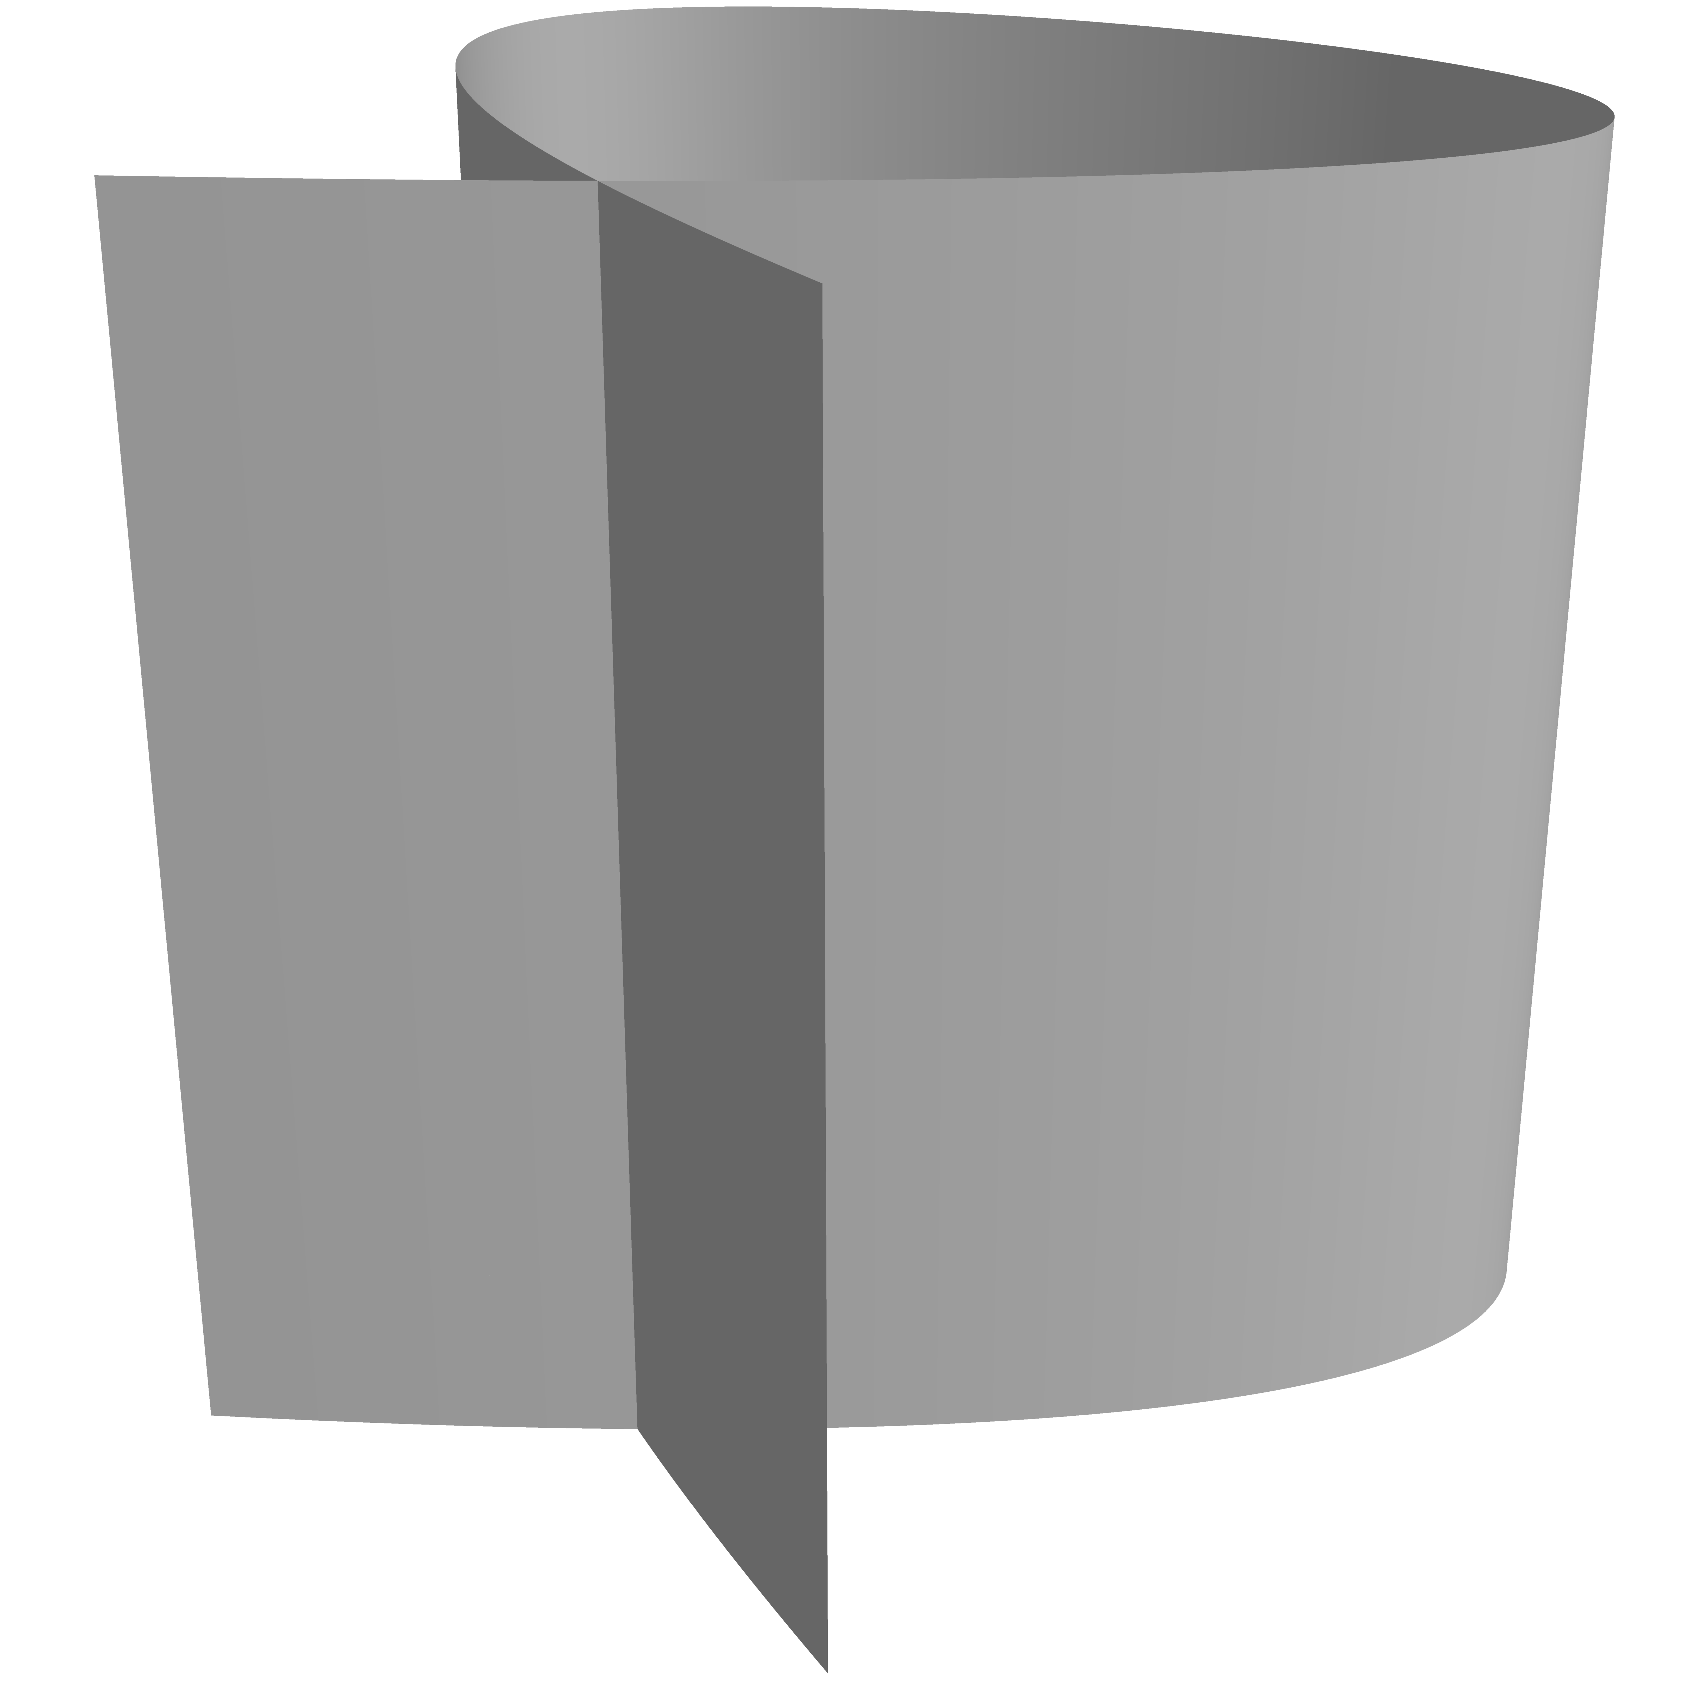
\includegraphics[width=4cm]{cylinder-on-curve}
\end{center}

Suppose instead that \(\alpha\) is algebraic, say satisfying a polynomial equation \(f(z)=0\) with \(f(z)\) a polynomial with coefficients from \(k(C)\).
So each coefficient of \(f(z)\) is itself a rational function on \(C\).
Each such function is expressible as a rational function of \(x,y\).
Clearing denominators, we get a polynomial equation \(f(x,y,z)=0\) with coefficients in the underlying field \(k\).
The solutions form a surface in 3-dimensional space.
But the resulting surface depends on how we pick out rational functions of \(x,y\) to represent our coefficients of \(f(z)\) from \(k(C)\).
So in fact we have to restrict our \(x,y\) variables to lie in \(C\), i.e. we consider the \emph{curve} \(D\) cut out by the equations \(p(x,y)=f(x,y,z)=0\).
\begin{center}
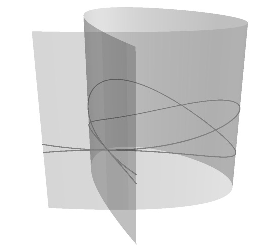
\includegraphics[width=4cm]{cylinder-on-curve-2}
\end{center}
The map \(\pr{x,y,z} \in D \mapsto \pr{x,y} \in C\) is regular.

We wonder now whether there is a \(k(C)\)-root to \(f(z)=0\), say \(\beta\).
This \(\beta\) is in \(k(C)\), so a rational function on \(C\), so that \(f(\beta)=0\).
So this is a rational map \(z=\beta(x,y)\) from \(C\) to \(D\), lifting the curve \(C\) up from the plane into space, tracing out \(D\) on the cylinder.
In particular, there is no such map if \(D\) is irreducible and \(D \to C\) is many to one:
\begin{center}
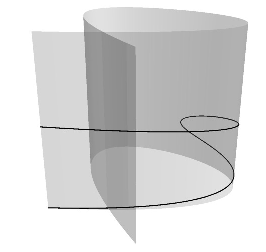
\includegraphics[width=4cm]{cylinder-on-curve-3}
\end{center}
So in such a case, \(k(C) \subset k(D)\) is a nontrivial field extension.
We get a picture giving some intuition for nontrivial algebraic field extensions: typically we expect to see an irreducible curve \(D\) mapping to a curve \(C\) by a many-to-one map.

The story continues similarly in higher dimensions: a transcendental extension increases dimension, while an algebraic extension, say of degree \(n\), preserves dimension, giving a new geometric object which maps regularly to the old one, by an \(n\)-to-\(1\) map.

   
\section{Rational curves}

Recall that the \emph{degree}\SubIndex{degree!of field extension} of a field extension \(k \subset K\), denoted \([K:k]\), is the smallest integer \(n\) so that there are \(n\) elements \(\alpha_1, \alpha_2, \dots, \alpha_n\) of \(K\) so that every element of \(K\) is a linear combination \(\sum a_j \alpha_j\) with coefficients \(a_1, a_2, \dots, a_n\) in \(k\).
The degree of the field extension is infinite if there is no such integer \(n\).

\begin{problem}{algebraic.curves:degree.multiplies}
Suppose that \(k \subset K \subset L\) are field extensions.
Prove that \([L:k]=[L:K][K:k]\).
Note: this works even if one or more degree is infinite: let \(n\infty=\infty n = \infty \infty = \infty\) for any positive integer \(n\).
You have to prove these infinite degree cases as well.
\end{problem}

\begin{problem}{algebraic.curves:degree.one}
Prove that a field extension is an isomorphism if and only if it has degree one.
\end{problem}
\begin{answer}{algebraic.curves:degree.one}
Take a basis consisting of one element \(\alpha \in K\).
Then \(1 \in K\) is somehow a multiple \(1=a \alpha\) for some \(a \in k\) so \(\alpha=1/a \in k\).
Any element \(\beta\) of \(K\) is \(\beta=c \alpha\) for some \(c \in k\) so \(\beta \in k\).
\end{answer}

\begin{problem}{algebraic.curves:find.degree}
Suppose that \(p(x)\) is an irreducible polynomial over a field \(k\).
Let \(K\defeq k[x]/(p(x))\).
Prove that \([K:k]\) is the degree of \(p(x)\).
\end{problem}
\begin{answer}{algebraic.curves:find.degree}
Let \(n\) be the degree of \(p(x)\).
We write each element \(b(x)\) in  \(k[x]\) as a polynomial, but if the polynomial has degree \(n\) or more, rewrite it as \(b(x)=q(x)p(x)+r(x)\), quotient and remainder. Then every element of \(K\) is written as the remainder term, i.e. as a polynomial of degree at most \(n-1\).  Hence the elements \(1,x,\dots,x^{n-1}\) in \(k[x]\) map to a spanning set inside \(K\). If not a basis, then there must be some linear relation between them, i.e. a lower degree polynomial in \(x\) vanishing in \(K\), i.e. vanishing modulo \(p(x)\).
But then taking quotient and remainder, we see that this is not possible.
Hence \(K\) has a basis over \(k\) consisting of the images of \(1,x,x^2,\dots,x^{n-1}\) in \(k[x]\).
\end{answer}


\begin{problem}{algebraic.curves:infinitely.many.points.on.trace}
Prove that if \(u(t)\) is a nonconstant rational function over a field \(k\), then there are infinitely many values of \(u(t)\) as \(t\) varies over \(\bar{k}\).
In particular, \(k \subset k(u(t))\) is a transcendental extension.
\end{problem}

Recall that a curve \(C=(0=f(x,y))\) is \emph{irreducible}
\SubIndex{irreducible!polynomial}%
\SubIndex{reducible!polynomial}% 
\SubIndex{polynomial!irreducible}%
\SubIndex{polynomial!reducible}
if \(f(x,y)\) is irreducible.

\begin{theorem}
An irreducible plane algebraic curve \(C\) is rational just when there is a nonconstant rational map \(L \to C\).
In other words, \(C\) is rational just when there are rational functions \(x(t),y(t)\) for which the point \((x(t),y(t))\) lies in \(C\) for all \(t\) in the algebraic closure of the field.
\end{theorem}
\begin{proof}
If our curve \(C\) is rational then by definition \(C\) is birational to a line, so there is such a map.
Suppose on the other hand that there is such a map \(L \to C\), say written as \(t \in L \mapsto (x(t),y(t)) \in C\) with
\[
f(x(t),y(t))=0
\]
for some rational functions \(x(t), y(t)\), not both constant.
As we vary \(t\) through \(\bar{k}\), the moving point \((x(t),y(t))\) moves through infinitely many different points of the plane.
Take a rational function on \(C\), say \(g(x,y)=b(x,y)/c(x,y)\).
Then \(c(x,y)\ne 0\) at all but finitely points of \(C\).
(Note that this requires that our curve \(C\) is irreducible, as otherwise we might have \(g(x,y)\) vanishing on a component of \(C\).)
So at infinitely many values of \(t\), \(g(x(t),y(t))\) is defined.
We map \(g(x,y) \in k(X) \mapsto g(x(t),y(t)) \in k(t)\), a morphism of fields. 
The image is some subfield \(K=k(x(t),y(t)) \subset k(t)\).
The result follows from the following theorem applied to \(K\).
\end{proof}

\begin{theorem}[L\"uroth's theorem]\define{Luroth's theorem@L\"uroth's theorem}\define{theorem!Luroth@L\"uroth}
Suppose that \(K \subset k(t)\) is a finitely generated extension of a field \(k\), where \(t\) is an abstract variable.
Then \(K=k(f(t))\) is generated by a single rational function \(f(t)\) in \(k(t)\).
In particular, either \(K=k\) (if \(f(t)\) is a constant function) or \(K\) is isomorphic to \(k(t)\) by \(t \mapsto f(t)\).
\end{theorem}
The proof of this theorem requires a lemma:
\begin{lemma}
Take a nonconstant rational function \(f(x)=b(x)/c(x)\), with \(b(x), c(x)\) coprime, over a field \(k\).
Then, as a polynomial in a variable \(y\) with coefficients in \(k(f(x))\), the expression
\[
f(x)c(y)-b(y) 
\]
in \(k(f(x))[y]\) is irreducible.
\end{lemma}
\begin{proof}
This expression is not zero, because it is nonconstant in \(x\).
It vanishes at \(y=x\).
Hence \(x\) satisfies this polynomial (in \(y\)) expression with coefficients in \(k(f(x))\).
So \(k(x)\) is an algebraic extension of \(k(f(x))\).
Since \(k(x)\) is transcendental over \(k\), \(k(f(x))\) is transcendental over \(k\).
So \(f(x)\) solves no polynomial equation over \(k\), and so taking any abstract variable \(t\) and mapping \(k(t,y) \to k(f(x),y)\) by \(t \mapsto f(x)\) gives an isomorphism of fields, and similarly \(k[t,y] \to k[f(x),y]\) is an isomorphism of rings.
By Gauss's lemma (proposition~\vref{proposition:Gauss.lemma}), to show that \(tc(y)-b(y)\) is irreducible in \(k(t)[y]\), it suffices to prove that it is irreducible in \(k[t,y]\), i.e. clear \(t\) from denominators.
If we can factor \(tc(y)-b(y)=g(t,y)h(t,y)\) in \(k[t,y]\) then one of \(g(t,y)\) or \(h(t,y)\) has degree 1 in \(t\), since the product does, and so one of \(g(t,y)\) or \(h(t,y)\) has degree zero in \(t\), depending only on \(y\), say \(g(t,y)=g(y)\).
Then \(g(t)h(t,y)=tc(y)-b(y)\), so \(g(y)\) divides \(tc(y)-b(y)\), and since \(t\) is an abstract variable, \(g(y)\) divides \(b(y)\) and \(c(y)\), which are coprime, so \(g(y)\) is a nonzero constant.
\end{proof}

We now prove L\"uroth's theorem:
\begin{proof}
For each element \(f(t)=b(t)/c(t)\) in \(K\), let \(n\) be the  larger of the degrees of \(b(t),c(t)\).
Pick an element \(f(t)=b(t)/c(t)\) in \(K\), not in \(k\), for which the value of \(n\) is as small as possible.
By the previous lemma, the polynomial \(B(y)=f(x)c(y)-b(y)\) is irreducible in \(k(f(x))[y]\), so the map
\[
x,y \in k(f(x))[y]/(B(y)) \mapsto x,x \in k(x)
\]
is an isomorphism of fields and \([k(x):k(f(x))]=n\).
The expression \(B(y)\) is the polynomial in \(K[y]\) of smallest positive \(y\)-degree which is satisfied by \(y=x\), since a smaller degree one would give a smaller value for \(n\).
Indeed the \(y\)-degree of \(B(y)\) is \(n\).
In particular, \(B(y)\) is also irreducible in \(K[y]\) and the map
\[
x,y \in K[y]/(B(y)) \mapsto x,x \in k(x)
\]
is an isomorphism.
In particular, \([k(x):K]=n\).
But
\begin{align*}
n
&=[k(x):k(f(x))],
\\
&=[k(x):K][K:k(f(x))],
\\
&=n[K:k(f(x))]
\end{align*}
so \([K:k(f(x))]=1\).
\end{proof}
   
   
\chapter{The projective plane}\label{chapter:projective.plane}
\epigraph[author={Arthur Cayley}]{The more systematic course in the present introductory memoir \dots
would have been to ignore altogether the notions of distance and
metrical geometry \dots. Metrical geometry is a part of descriptive
geometry, and descriptive geometry is all geometry.}\SubIndex{Cayley, Arthur}
The old fashioned term \emph{descriptive geometry}\define{descriptive geometry} means the geometry of straight lines.
Straight lines in the plane remain straight when you rescale the plane, or translate the plane to the left or right, up or down, or when you rotate the plane.
They even remain straight when you carry out any linear change of variables, as you know from linear algebra.

\bigskip

\epigraph[author={William Blake}, source={Auguries of Innocence}]{To see a World in a Grain of Sand, \\ And Heaven in a Wild Flower. \\ Hold Infinity in the palm of your hand, \\ And Eternity in an hour.}\SubIndex{Blake, William}

Railway tracks built on a flat plane appear to meet ``at infinity''.
\begin{center}
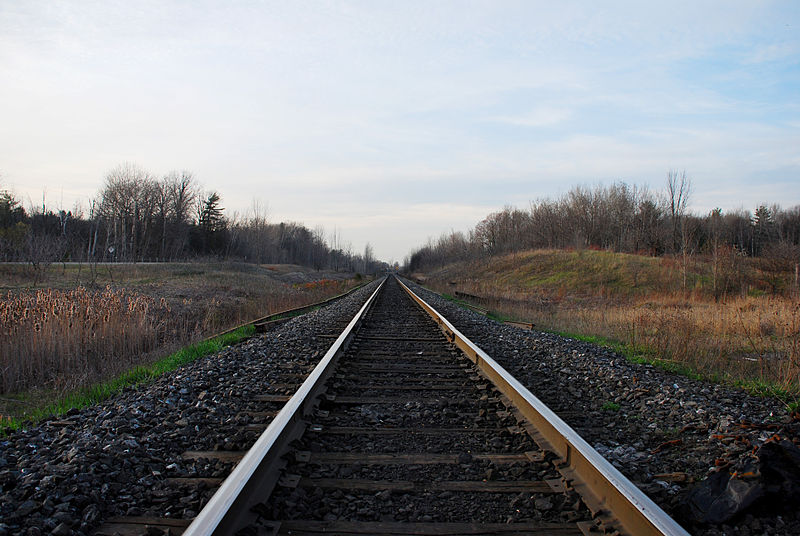
\includegraphics[width=4cm]{railway-tracks.jpg} \\[2pt]
\begin{minipage}{4cm}\raggedright\tiny{Creative Commons Attribution-Share Alike 3.0 Unported license. I, MarcusObal}\end{minipage}
\end{center}
Imagine that we were to add a point to the plane ``at infinity'' in the direction where these tracks (straight lines) appear to meet.
\emph{Danger:} in order to add only one point, imagine that the two rails meet at the \emph{same} point in one direction as they do in the other, making them both into circles.
The projective plane is the set of all of the usual points of the plane (which we can think of as the ``finite points'' of the projective plane) together with some sort of ``points at infinity'' to represent the directions in the plane.

\epigraph[author={Fyodor Dostoyevsky}, source={The Brothers Karamazov}]{
But you must note this: if God exists and if He really did
create the world, then, as we all know, He created it according to
the geometry of Euclid and the human mind with the conception
of only three dimensions in space.  Yet there have been and
still are geometricians and philosophers, and even some of the
most distinguished, who doubt whether the whole universe, or
to speak more widely the whole of being, was only created in
Euclid's geometry; they even dare to dream that two parallel
lines, which according to Euclid can never meet on earth, may
meet somewhere in infinity.}\SubIndex{Dostoyevsky, Fyodor}\SubIndex{Brothers Karamazov}


We would like a more precise mathematical definition of points ``at infinity''.
A \emph{pencil}\define{pencil} of parallel lines is the collection of all lines parallel to a given line:
\[
\begin{tikzpicture}
\clip (0,0) rectangle (1,1);
\foreach \i in {-1,-0.9,...,1} 
{
	\draw (0,{\i}) -- (1,{\i+1});
}
\end{tikzpicture}
\]
A simple approach: just say that a ``point at infinity'' means nothing more than a choice of pencil of parallel lines.

There is another completely different way to give a precise mathematical definition of the projective plane, which is more geometric and more powerful.
Place yourself at a vantage point above the plane.
\begin{center}
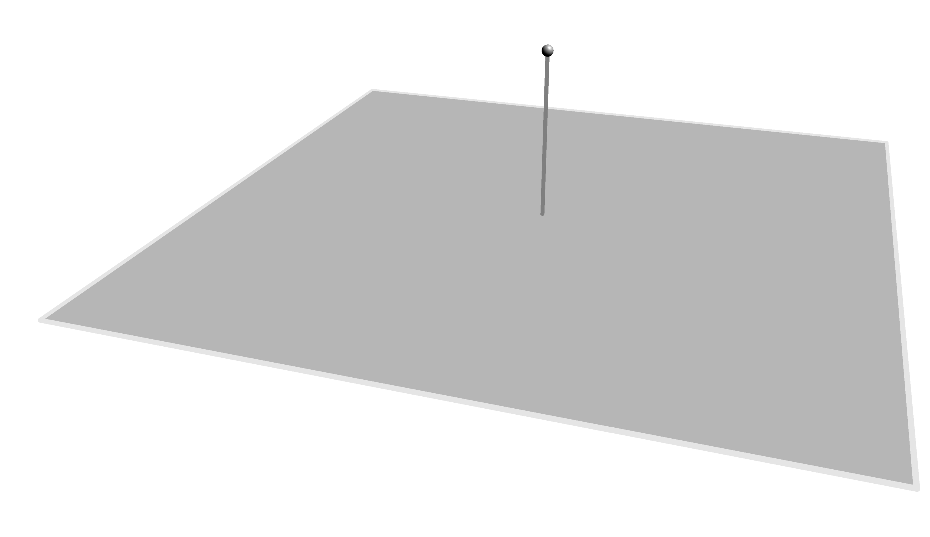
\includegraphics[width=4cm]{above-the-plane-vantage}
\end{center}
Every ``finite'' point of the plane lies on a line through your vantage point: the line of sight.
\begin{center}
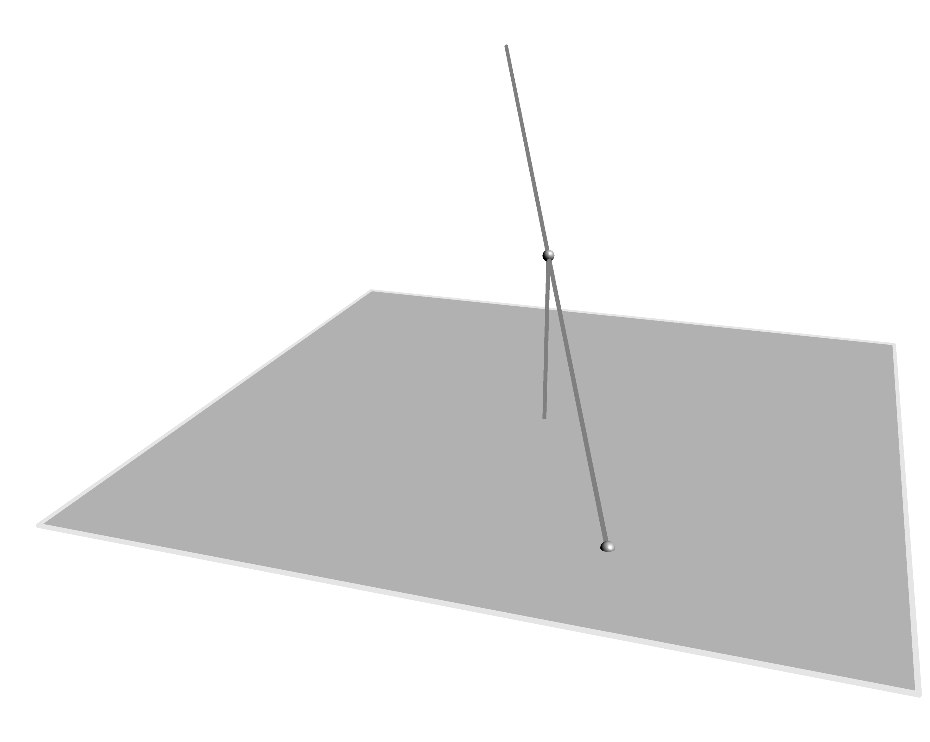
\includegraphics[width=4cm]{above-the-plane-connect}
\end{center}
You can also look out to the points at infinity, along lines:
\begin{center}
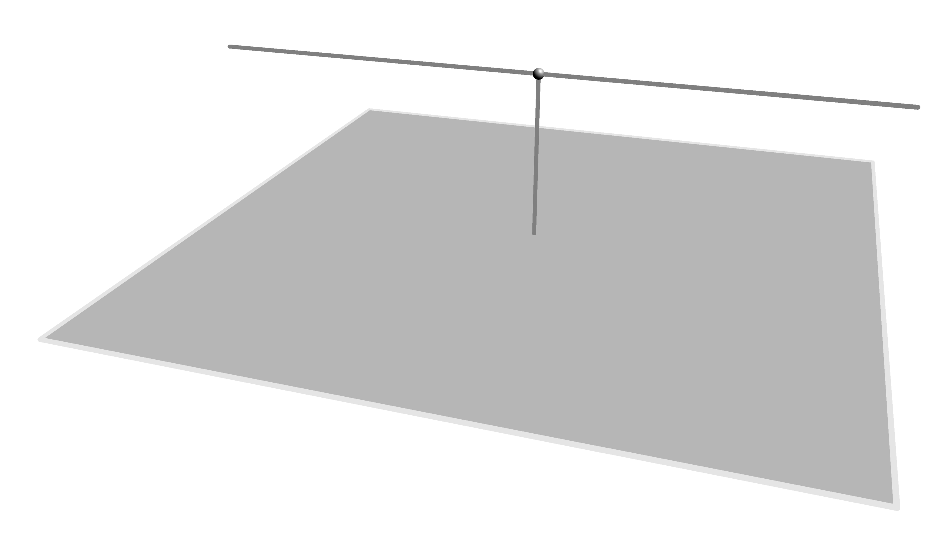
\includegraphics[width=4cm]{above-the-plane-off-to-infinity}
\end{center}
For example, there is such a line  parallel to the lines of our train track:
\begin{center}
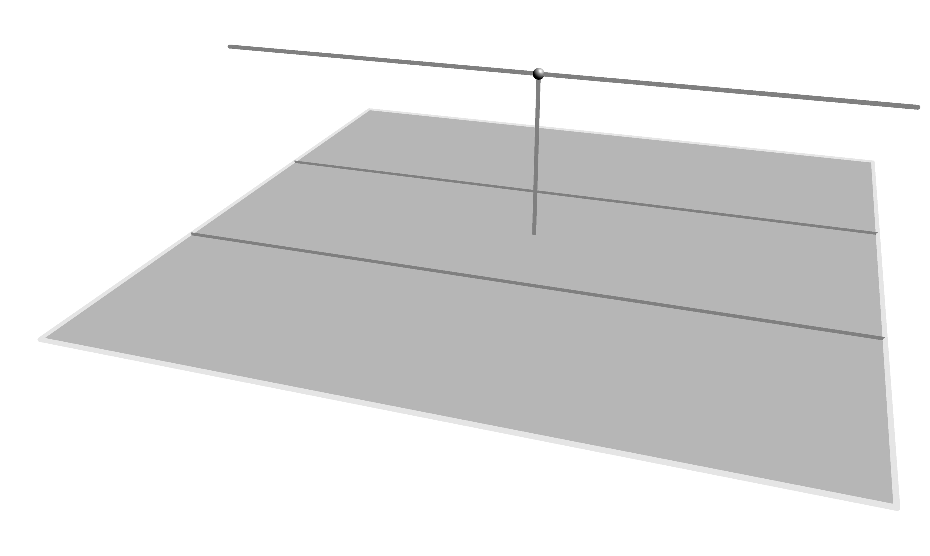
\includegraphics[width=4cm]{above-the-plane-3}
\end{center}

On the other hand, if we take any line through the vantage point, either it hits a ``finite'' point of the plane:
\begin{center}
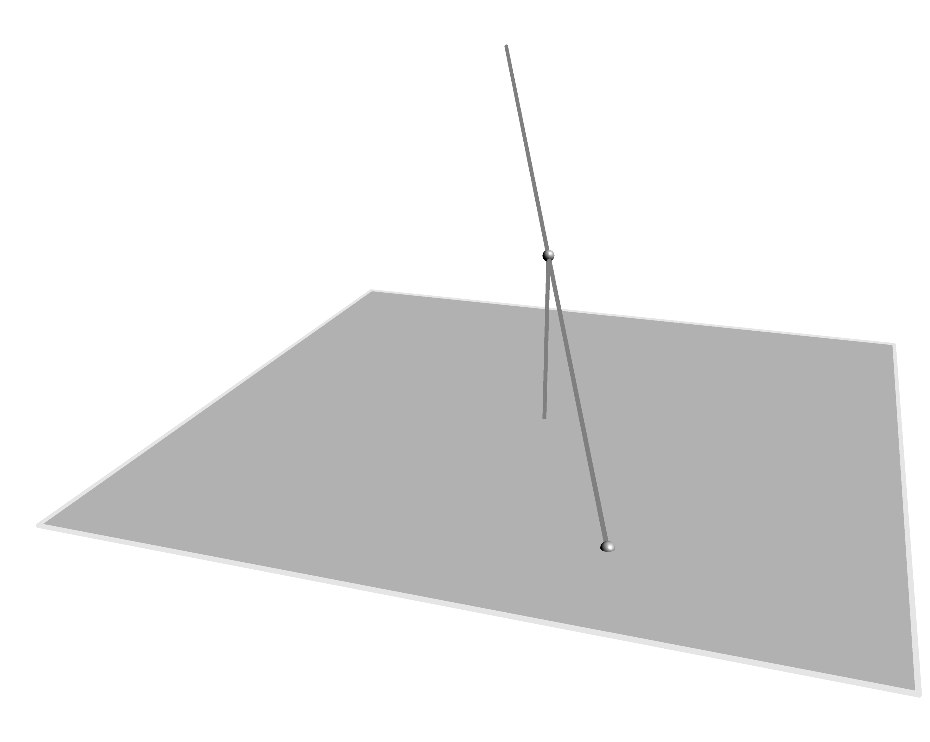
\includegraphics[width=4cm]{above-the-plane-connect}
\end{center}
or it is parallel to the plane
\begin{center}
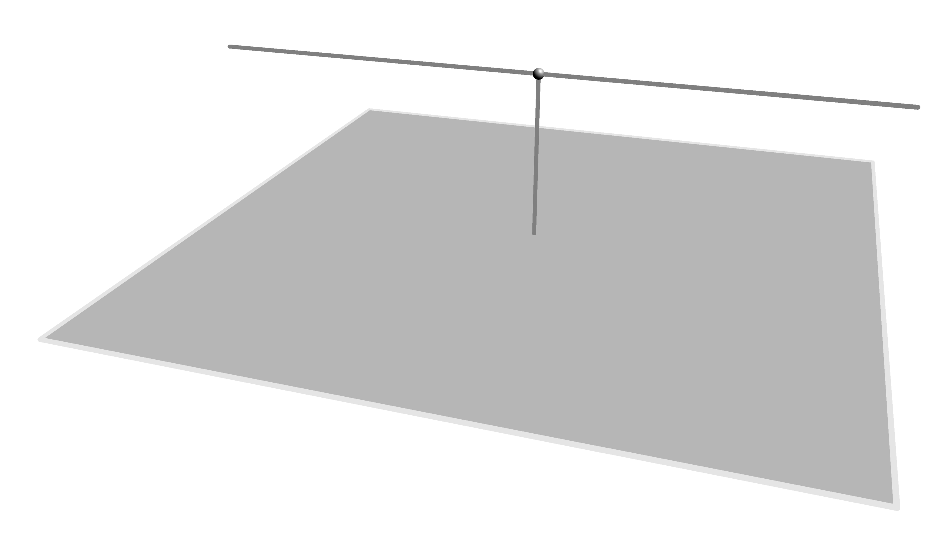
\includegraphics[width=4cm]{above-the-plane-off-to-infinity}
\end{center}
so that it is pointed along the direction of some train tracks (lines) in the plane, to some ``point at infinity''.
\begin{center}
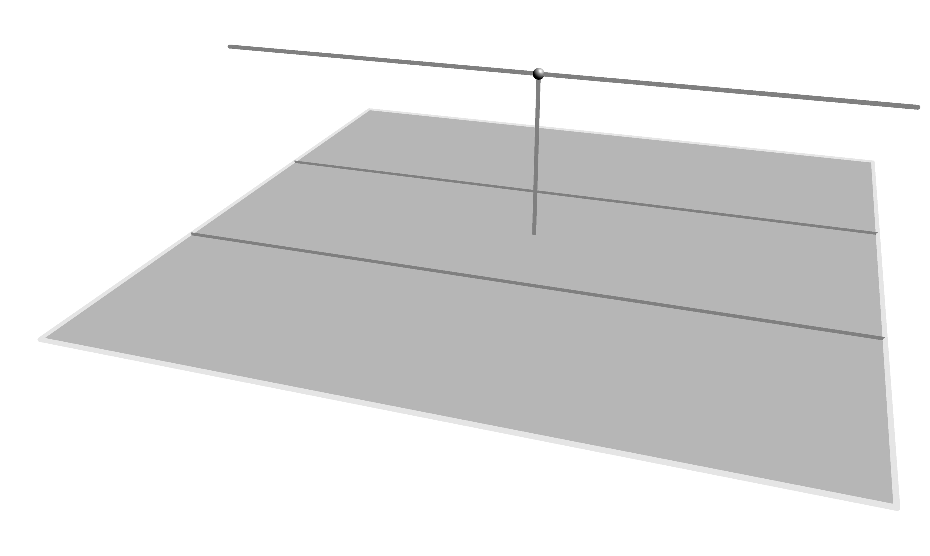
\includegraphics[width=4cm]{above-the-plane-3}
\end{center}
The points of the projective plane, finite points together with infinite points at infinity, are in 1-1 correspondence with lines through the vantage point.

This picture gives us a rigorous definition of points at infinity: the \emph{projective plane}\define{projective!plane} is the set of all lines through a chosen point of 3-dimensional space, called the vantage point.
The \emph{points} of the projective plane (using this definition) are the lines through the vantage point.
The ``finite points'' are the lines not parallel to the horizontal plane, while the ``infinite points'' are the lines which are parallel the horizontal plane.
The \emph{lines}\define{projective!line}, also called \emph{projective lines}, of the projective plane are the planes through the vantage point.




\section{Homogeneous coordinates}
We can make this more explicit by writing each point of 3-dimensional space \(\R{3}\) as a triple \((x,y,z)\).
Draw the plane not as the usual \(xy\)-plane, but as the plane \(z=z_0\), for some nonzero constant \(z_0\).
Take the vantage point to be the origin.
Any linear change of the 3 variables \(x,y,z\) takes lines (and planes) through the origin to one another: there are more symmetries of the projective plane than we encountered before.

Every point of 3-dimensional space not at the origin lies on a unique line through the origin.
So every point \((x,y,z)\) with not all of \(x,y,z\) zero lines on a unique line through the origin.
The points of this line are precisely the rescalings \((tx,ty,tz)\) of that point.
So each point of the projective plane can be written as a triple \((x,y,z)\), not all zero, and two such triples represent the same point just when each is a rescaling of the other.
Denote such a point as \([x,y,z]\).
For example, the point \([3,1,2]\) of the projective plane means the line through the origin consisting of the points of the form \((3t,t,2t)\) for all values of a variable \(t\), including \((3,1,2)\), \((3 \cdot 2, 1 \cdot 2, 2 \cdot 2)\), \((-3,-1,-2)\), and so on.
We write this as:
\[
[3,1,2]=[3 \cdot 2, 1 \cdot 2, 2 \cdot 2]=[-3,-1,-2].
\]
The coordinates \(x,y,z\) are the \emph{homogeneous coordinates}\define{homogeneous!coordinates}\define{coordinates!homogeneous} of a point \([x,y,z]\) of the projective plane.

In our pictures, the plane \(z=z_0\) was below the vantage point, but it is more traditional to take the plane to be \(z=1\), above the vantage point.
The \emph{affine plane} is just the usual \(xy\) plane, but identified either with the plane \(z=1\), or with the subset of the projective plane given by points \([x,y,1]\).

The roles of \(x,y,z\) are all the same now, and we can see that any linear change of variables of \(x,y,z\) takes the points of the projective plane to one another, and takes the lines of the projective plane to one another.
Each linear change of variables is represented by an invertible matrix
\[
g=
\begin{pmatrix}
g_{00} & g_{01} & g_{02} \\
g_{10} & g_{11} & g_{12} \\
g_{20} & g_{21} & g_{22}
\end{pmatrix}.
\]
Conventionally we label our matrix columns using \(0,1,2\) rather than \(1,2,3\).
Such a matrix takes a point \(p=[x,y,z]\) of the plane to the point \(q=[X,Y,Z]\) where
\[
\begin{pmatrix}
X \\
Y \\
Z
\end{pmatrix}
=
g
\begin{pmatrix}
x \\
y \\
z
\end{pmatrix}.
\]
We denote this relation as \(q=[g]p\) and call \([g]\) a \emph{projective automorphism}\define{projective!automorphism}.
Clearly if \(g\) and \(h\) are 2 invertible \(3 \times 3\) matrices, then \([gh]=[g][h]\), i.e. we carry out the transformation of lines through the origin by carrying out the multiplications by the matrices.

\begin{lemma}
If a square matrix \(g\) rescales every nonzero vector by a scalar, i.e. \(gx=\lambda(x)x\) for some number \(\lambda(x)\), for every vector \(x \ne 0\), then \(\lambda(x)\) is a constant scalar independent of \(x\).
\end{lemma}
\begin{proof}
Suppose that \(g\) is \(n \times n\).
If \(n=1\) then every square matrix is a constant scalar, so suppose that \(n \ge 2\).
Write our vectors as \(x=\sum_j x_j e_j\) in the standard basis of \(\R{n}\) and calculate
\begin{align*}
gx
&=
\lambda\of{x} x,
\\
&=
\sum_j \lambda\of{x} x_j e_j,
\\
&=
\sum_j x_j ge_j,
\\
&=
\sum_j x_j \lambda\of{e_j} e_j.
\end{align*}
So for any \(x\) with \(x_j\ne 0\), we have \(\lambda(x)=\lambda\of{e_j}\).
But then if \(x_i \ne 0\), and if \(i \ne j\), then
\begin{align*}
\lambda(x) 
&=
\lambda\of{e_i},
\\
&=
\lambda\of{e_i+e_j},
\\
&=
\lambda\of{e_j}.
\end{align*}
So \(\lambda\) is a constant.
\end{proof}

\begin{lemma}
Two projective automorphisms \([g],[h]\) have precisely the same effect on all points \([x,y,z]\) of the projective plane just when the matrices agree up to a constant \(h=\lambda g\), some number \(\lambda \ne 0\).
\end{lemma}
\begin{proof}
Let \(\ell\defeq h^{-1}g\), so that \([\ell]=[h]^{-1}[g]\) and \([\ell]\) fixes every point of the projective plane just when \(\ell\) rescales every vector in \(\R{3}\) by  a scalar.
\end{proof} 

In particular, the points of the projective plane are permuted by the projective automorphisms, as are the projective lines.

The \emph{projective plane}\define{projective!plane} over any field \(k\), denoted \(\Proj[2]{k}\),\Notation{P2k}{\Proj[2]{k}}{projective plane over a field \(k\)} is the set of lines through the origin in \(k^3\).
In \(k^3\), the line through two points 
\[
p=
\begin{pmatrix}
x \\
y \\
z
\end{pmatrix},
q=
\begin{pmatrix}
X \\
Y \\
Z
\end{pmatrix}
\]
is just the set of all points \(tp+(1-t)q\) for \(t\) in \(k\).

\section{Example: the Fano plane}

Let \(k\defeq \Zmod{2}\); the \emph{Fano plane}\define{Fano plane}\define{plane!Fano} is the projective plane \(\Proj[2]{k}\).
Each point is \([x,y,z]\) with \(x,y,z\) in \(k\) defined up to rescaling.
But the only nonzero scalar you can use to rescale with is \(1\), since \(k=\Set{0,1}\).
Therefore we can just write \([x,y,z]\) as \((x,y,z)\).
Taking all possibilities for \(x,y,z\) from \(k\), not all zero, we get 7 points
\[
\begin{bmatrix}
1 \\
0 \\
0
\end{bmatrix},
\begin{bmatrix}
0 \\
1 \\
0
\end{bmatrix},
\begin{bmatrix}
1 \\
1 \\
0
\end{bmatrix},
\begin{bmatrix}
0 \\
0 \\
1
\end{bmatrix},
\begin{bmatrix}
1 \\
0 \\
1
\end{bmatrix},
\begin{bmatrix}
0 \\
1 \\
1
\end{bmatrix},
\begin{bmatrix}
1 \\
1 \\
1
\end{bmatrix},
\]
corresponding to the numbers \(1,2, \dots, 7\) written in base \(2\).

We can also draw this diagram as a cube; for each point, you draw the corresponding point in \(\R{3}\) with the same coordinates:
\begin{center}
\newcommand{\Depth}{1}
\newcommand{\Height}{1}
\newcommand{\Width}{1}
\tdplotsetmaincoords{70}{110}
\begin{tikzpicture}[tdplot_main_coords]
\coordinate (0) at (0,0,0);
\coordinate (1) at (\Depth,0,\Height);
\coordinate (2) at (\Depth,\Width,0);
\coordinate (3) at (0,\Width,\Height);
\coordinate (4) at (\Depth,\Width,\Height);
\coordinate (5) at (0,\Width,0);
\coordinate (6) at (0,0,\Height);
\coordinate (7) at (\Depth,0,0);

\draw[gray!10,fill=gray!10] (0) -- (6) -- (1) -- (7) -- cycle;% Left Face
\draw[gray!10,fill=gray!30] (0) -- (7) -- (2) -- (5) -- cycle;% Bottom Face
\draw[gray!10,fill=gray!40] (0) -- (6) -- (3) -- (5) -- cycle;% Back Face
\draw[gray!10,fill=gray!20,opacity=0.6] (1) -- (4) -- (2) -- (7) -- cycle;% Front Face
\draw[gray!10,fill=gray!20,opacity=0.8] (1) -- (4) -- (3) -- (6) -- cycle;% Top Face
\draw[gray!10,fill=gray!20,opacity=0.8] (4) -- (3) -- (5) -- (2) -- cycle;% Right Face

\node at (1) {\small\(6\)};
\node at (2) {\small\(3\)};
\node at (3) {\small\(5\)};
\node at (4) {\small\(7\)};
\node at (5) {\small\(1\)};
\node at (6) {\small\(4\)};
\node at (7) {\small\(2\)};

%% Following is for debugging purposes so you can see where the points are
%% These are last so that they show up on top
%\foreach \xy in {O, A, B, C, D, E, F, G}{
%    \node at (\xy) {\xy};
%}
\end{tikzpicture}
\end{center}
with one vertex not marked.
The unmarked vertex 
If we let \(k\defeq\Zmod{2}\), then the cube is the set of points in \(k^3\), or more precisely, since the unlabelled point is the origin and is deleted, the cube is the Fano plane.
Every line in the Fano plane has three vertices.
Take two numbers from 1 to 7, say \(1, 5\), and write out their binary digits under one another:
\[
\begin{array}{@{}c@{}c@{}c@{}}
0&0&1\\
1&0&1
\end{array}.
\]
Look at these as vectors in \(k^3\), so add them without carrying digits:
\[
\begin{array}{@{}c@{}c@{}c@{}}
0&0&1\\
1&0&1\\ \midrule
1&0&0
\end{array}
\]
The sum vector lies on the same line in the Fano plane, giving the lines:
\begin{center}
\newcommand{\Depth}{1}
\newcommand{\Height}{1}
\newcommand{\Width}{1}
\tdplotsetmaincoords{70}{110}
\begin{tikzpicture}[tdplot_main_coords]%Highlight the bottom
\coordinate (0) at (0,0,0);
\coordinate (1) at (\Depth,0,\Height);
\coordinate (2) at (\Depth,\Width,0);
\coordinate (3) at (0,\Width,\Height);
\coordinate (4) at (\Depth,\Width,\Height);
\coordinate (5) at (0,\Width,0);
\coordinate (6) at (0,0,\Height);
\coordinate (7) at (\Depth,0,0);
%

\draw[gray!10,fill=gray!10] (0) -- (6) -- (1) -- (7) -- cycle;% Left Face
\draw[gray!10,fill=gray!110] (0) -- (7) -- (2) -- (5) -- cycle;% Bottom Face
\draw[gray!10,fill=gray!40] (0) -- (6) -- (3) -- (5) -- cycle;% Back Face
\draw[gray!10,fill=gray!20,opacity=0.6] (1) -- (4) -- (2) -- (7) -- cycle;% Front Face
\draw[gray!10,fill=gray!20,opacity=0.8] (1) -- (4) -- (3) -- (6) -- cycle;% Top Face
\draw[gray!10,fill=gray!20,opacity=0.8] (4) -- (3) -- (5) -- (2) -- cycle;% Right Face

\node at (1) {\small\(6\)};
\node at (2) {\small\(3\)};
\node at (3) {\small\(5\)};
\node at (4) {\small\(7\)};
\node at (5) {\small\(1\)};
\node at (6) {\small\(4\)};
\node at (7) {\small\(2\)};

%% Following is for debugging purposes so you can see where the points are
%% These are last so that they show up on top
%\foreach \xy in {O, A, B, C, D, E, F, G}{
%    \node at (\xy) {\xy};
%}
\end{tikzpicture}
\begin{tikzpicture}[tdplot_main_coords]%Highlight the left
\coordinate (0) at (0,0,0);
\coordinate (1) at (\Depth,0,\Height);
\coordinate (2) at (\Depth,\Width,0);
\coordinate (3) at (0,\Width,\Height);
\coordinate (4) at (\Depth,\Width,\Height);
\coordinate (5) at (0,\Width,0);
\coordinate (6) at (0,0,\Height);
\coordinate (7) at (\Depth,0,0);
%

\draw[gray!10,fill=gray!90] (0) -- (6) -- (1) -- (7) -- cycle;% Left Face
\draw[gray!10,fill=gray!30] (0) -- (7) -- (2) -- (5) -- cycle;% Bottom Face
\draw[gray!10,fill=gray!40] (0) -- (6) -- (3) -- (5) -- cycle;% Back Face
\draw[gray!10,fill=gray!20,opacity=0.6] (1) -- (4) -- (2) -- (7) -- cycle;% Front Face
\draw[gray!10,fill=gray!20,opacity=0.8] (1) -- (4) -- (3) -- (6) -- cycle;% Top Face
\draw[gray!10,fill=gray!20,opacity=0.8] (4) -- (3) -- (5) -- (2) -- cycle;% Right Face

\node at (1) {\small\(6\)};
\node at (2) {\small\(3\)};
\node at (3) {\small\(5\)};
\node at (4) {\small\(7\)};
\node at (5) {\small\(1\)};
\node at (6) {\small\(4\)};
\node at (7) {\small\(2\)};

%% Following is for debugging purposes so you can see where the points are
%% These are last so that they show up on top
%\foreach \xy in {O, A, B, C, D, E, F, G}{
%    \node at (\xy) {\xy};
%}
\end{tikzpicture}
\begin{tikzpicture}[tdplot_main_coords]%Highlight back face
\coordinate (0) at (0,0,0);
\coordinate (1) at (\Depth,0,\Height);
\coordinate (2) at (\Depth,\Width,0);
\coordinate (3) at (0,\Width,\Height);
\coordinate (4) at (\Depth,\Width,\Height);
\coordinate (5) at (0,\Width,0);
\coordinate (6) at (0,0,\Height);
\coordinate (7) at (\Depth,0,0);
%

\draw[gray!10,fill=gray!10] (0) -- (6) -- (1) -- (7) -- cycle;% Left Face
\draw[gray!10,fill=gray!30] (0) -- (7) -- (2) -- (5) -- cycle;% Bottom Face
\draw[gray!10,fill=gray!120] (0) -- (6) -- (3) -- (5) -- cycle;% Back Face
\draw[gray!10,fill=gray!20,opacity=0.6] (1) -- (4) -- (2) -- (7) -- cycle;% Front Face
\draw[gray!10,fill=gray!20,opacity=0.8] (1) -- (4) -- (3) -- (6) -- cycle;% Top Face
\draw[gray!10,fill=gray!20,opacity=0.8] (4) -- (3) -- (5) -- (2) -- cycle;% Right Face

\node at (1) {\small\(6\)};
\node at (2) {\small\(3\)};
\node at (3) {\small\(5\)};
\node at (4) {\small\(7\)};
\node at (5) {\small\(1\)};
\node at (6) {\small\(4\)};
\node at (7) {\small\(2\)};

%% Following is for debugging purposes so you can see where the points are
%% These are last so that they show up on top
%\foreach \xy in {O, A, B, C, D, E, F, G}{
%    \node at (\xy) {\xy};
%}
\end{tikzpicture}
\begin{tikzpicture}[tdplot_main_coords]
\coordinate (0) at (0,0,0);
\coordinate (1) at (\Depth,0,\Height);
\coordinate (2) at (\Depth,\Width,0);
\coordinate (3) at (0,\Width,\Height);
\coordinate (4) at (\Depth,\Width,\Height);
\coordinate (5) at (0,\Width,0);
\coordinate (6) at (0,0,\Height);
\coordinate (7) at (\Depth,0,0);
%

\draw[gray!10,fill=gray!10] (0) -- (6) -- (1) -- (7) -- cycle;% Left Face
\draw[gray!10,fill=gray!30] (0) -- (7) -- (2) -- (5) -- cycle;% Bottom Face
\draw[gray!10,fill=gray!40] (0) -- (6) -- (3) -- (5) -- cycle;% Back Face
\draw[gray!10,fill=gray!20,opacity=0.6] (1) -- (4) -- (2) -- (7) -- cycle;% Front Face
\draw[gray!10,fill=gray!20,opacity=0.8] (1) -- (4) -- (3) -- (6) -- cycle;% Top Face
\draw[gray!10,fill=gray!20,opacity=0.8] (4) -- (3) -- (5) -- (2) -- cycle;% Right Face

\draw[gray!10,fill=gray!80,opacity=0.8] (0) -- (6) -- (4) -- (2) -- cycle;

\node at (1) {\small\(6\)};
\node at (2) {\small\(3\)};
\node at (3) {\small\(5\)};
\node at (4) {\small\(7\)};
\node at (5) {\small\(1\)};
\node at (6) {\small\(4\)};
\node at (7) {\small\(2\)};

%% Following is for debugging purposes so you can see where the points are
%% These are last so that they show up on top
%\foreach \xy in {O, A, B, C, D, E, F, G}{
%    \node at (\xy) {\xy};
%}
\end{tikzpicture}
\begin{tikzpicture}[tdplot_main_coords]
\coordinate (0) at (0,0,0);
\coordinate (1) at (\Depth,0,\Height);
\coordinate (2) at (\Depth,\Width,0);
\coordinate (3) at (0,\Width,\Height);
\coordinate (4) at (\Depth,\Width,\Height);
\coordinate (5) at (0,\Width,0);
\coordinate (6) at (0,0,\Height);
\coordinate (7) at (\Depth,0,0);
%

\draw[gray!10,fill=gray!10] (0) -- (6) -- (1) -- (7) -- cycle;% Left Face
\draw[gray!10,fill=gray!30] (0) -- (7) -- (2) -- (5) -- cycle;% Bottom Face
\draw[gray!10,fill=gray!40] (0) -- (6) -- (3) -- (5) -- cycle;% Back Face
\draw[gray!10,fill=gray!20,opacity=0.6] (1) -- (4) -- (2) -- (7) -- cycle;% Front Face
\draw[gray!10,fill=gray!20,opacity=0.8] (1) -- (4) -- (3) -- (6) -- cycle;% Top Face
\draw[gray!10,fill=gray!20,opacity=0.8] (4) -- (3) -- (5) -- (2) -- cycle;% Right Face

\draw[gray!10,fill=gray!80,opacity=0.8] (0) -- (1) -- (4) -- (5) -- cycle;

\node at (1) {\small\(6\)};
\node at (2) {\small\(3\)};
\node at (3) {\small\(5\)};
\node at (4) {\small\(7\)};
\node at (5) {\small\(1\)};
\node at (6) {\small\(4\)};
\node at (7) {\small\(2\)};

%% Following is for debugging purposes so you can see where the points are
%% These are last so that they show up on top
%\foreach \xy in {O, A, B, C, D, E, F, G}{
%    \node at (\xy) {\xy};
%}
\end{tikzpicture}
{
\tdplotsetmaincoords{50}{110}
\begin{tikzpicture}[tdplot_main_coords]
\coordinate (0) at (0,0,0);
\coordinate (1) at (\Depth,0,\Height);
\coordinate (2) at (\Depth,\Width,0);
\coordinate (3) at (0,\Width,\Height);
\coordinate (4) at (\Depth,\Width,\Height);
\coordinate (5) at (0,\Width,0);
\coordinate (6) at (0,0,\Height);
\coordinate (7) at (\Depth,0,0);

\draw[gray!10,fill=gray!10] (0) -- (6) -- (1) -- (7) -- cycle;% Left Face
\draw[gray!10,fill=gray!30] (0) -- (7) -- (2) -- (5) -- cycle;% Bottom Face
\draw[gray!10,fill=gray!40] (0) -- (6) -- (3) -- (5) -- cycle;% Back Face
\draw[gray!10,fill=gray!20,opacity=0.6] (1) -- (4) -- (2) -- (7) -- cycle;% Front Face
\draw[gray!10,fill=gray!20,opacity=0.8] (1) -- (4) -- (3) -- (6) -- cycle;% Top Face
\draw[gray!10,fill=gray!20,opacity=0.8] (4) -- (3) -- (5) -- (2) -- cycle;% Right Face

\draw[gray!10,fill=gray!80,opacity=0.8] (0) -- (7) -- (4) -- (3) -- cycle;

\node at (1) {\small\(6\)};
\node at (2) {\small\(3\)};
\node at (3) {\small\(5\)};
\node at (4) {\small\(7\)};
\node at (5) {\small\(1\)};
\node at (6) {\small\(4\)};
\node at (7) {\small\(2\)};

%% Following is for debugging purposes so you can see where the points are
%% These are last so that they show up on top
%\foreach \xy in {O, A, B, C, D, E, F, G}{
%    \node at (\xy) {\xy};
%}
\end{tikzpicture}
}
\begin{tikzpicture}[tdplot_main_coords]
\coordinate (0) at (0,0,0);
\coordinate (1) at (\Depth,0,\Height);
\coordinate (2) at (\Depth,\Width,0);
\coordinate (3) at (0,\Width,\Height);
\coordinate (4) at (\Depth,\Width,\Height);
\coordinate (5) at (0,\Width,0);
\coordinate (6) at (0,0,\Height);
\coordinate (7) at (\Depth,0,0);

\draw[gray!10,fill=gray!10] (0) -- (6) -- (1) -- (7) -- cycle;% Left Face
\draw[gray!10,fill=gray!30] (0) -- (7) -- (2) -- (5) -- cycle;% Bottom Face
\draw[gray!10,fill=gray!40] (0) -- (6) -- (3) -- (5) -- cycle;% Back Face
\draw[gray!10,fill=gray!20,opacity=0.6] (1) -- (4) -- (2) -- (7) -- cycle;% Front Face
\draw[gray!10,fill=gray!20,opacity=0.8] (1) -- (4) -- (3) -- (6) -- cycle;% Top Face
\draw[gray!10,fill=gray!20,opacity=0.8] (4) -- (3) -- (5) -- (2) -- cycle;% Right Face

\draw[gray!10,fill=gray!80,opacity=0.8] (1) -- (3) -- (2) -- cycle;

\node at (1) {\small\(6\)};
\node at (2) {\small\(3\)};
\node at (3) {\small\(5\)};
%\node at (4) {\small\(7\)};
\node at (5) {\small\(1\)};
\node at (6) {\small\(4\)};
\node at (7) {\small\(2\)};
\end{tikzpicture}
\end{center}


\section{Projective space}

Similarly, \emph{projective space}\define{projective!space} \(\Proj[n]{k}\)\Notation{Pnk}{\Proj[n]{k}}{projective space over a field \(k\)} is the set of lines through the origin of \(k^{n+1}\), and a \emph{projective automorphism}\define{projective!automorphism} of projective space is the result of applying an invertible square matrix to those lines.
Again, two invertible square matrices yield the same projective automorphism just when they agree up to a scalar multiple, by the same proof.

\chapter{Algebraic curves in the projective plane}

\section{Homogenisation of plane curves}

Take an algebraic curve \(y^2=x^2+x^3\) in the affine plane over a field \(k\).
\begin{center}
\documentclass{standalone}
\usepackage{tikz}
\usepackage{pgfplots}
\usepackage{xparse}
\pgfplotsset{compat=1.14}%
\colorlet{curveZero}{gray!75}
\colorlet{curveOne}{blue!60}
\colorlet{curveTwo}{brown!50!gray}
\colorlet{curveThree}{green!40!gray}
\colorlet{curveFour}{red!50!gray}
\NewDocumentCommand\DrawDotInPlot{O{}mmO{}}%
{%
\fill[gray!20,draw=gray] (axis cs:{#2},{#3}) circle (1.3pt) node[above,black,#4] {\(#1\)};%
}%
\NewDocumentCommand\DrawDot{O{}mmO{}}%
{%
\fill[gray!20,draw=gray] ({#2},{#3}) circle (1.3pt) node[above,black,#4] {\(#1\)};%
}%
\NewDocumentCommand\DrawNode{O{}m}%
{%
\fill[gray!20,draw=gray] (#2) circle (1.3pt) node[above,black] {\(#1\)};%
}%
\colorlet{axisColor}{gray!50}
\tikzstyle{shapeZero}=[fill=curveZero,opacity=.4]
\tikzstyle{shapeOne}=[fill=curveOne,opacity=.4]
\tikzstyle{shapeTwo}=[fill=curveTwo,opacity=.4]
\tikzstyle{shapeThree}=[fill=curveThree,opacity=.4]
\tikzstyle{groupElementLabel}=[minimum size=2.4em]
\tikzstyle{groupElement}=[minimum size=2.4em,shapeZero,draw=curveZero]
\tikzstyle{cosetOne}=[minimum size=2.4em,shapeOne,draw=curveOne]
\tikzstyle{cosetTwo}=[minimum size=2.4em,shapeTwo,draw=curveTwo]


\begin{document}
\begin{tikzpicture}
\begin{axis}[hide axis,xmin=-2,xmax=2,ymin=-2,ymax=2,width=4cm]
  \addplot[very thick,domain=-1:0,curveZero,samples=200]{sqrt(x^2+x^3)};%
  \addplot[very thick,domain=-1:0,curveZero,samples=200]{-sqrt(x^2+x^3)};%
  \addplot[very thick,domain=0:1,curveZero]{sqrt(x^2+x^3)};%
  \addplot[very thick,domain=0:1,curveZero]{-sqrt(x^2+x^3)};%
\end{axis}
\end{tikzpicture}
\end{document}

\end{center}
The \emph{cone}\define{cone} on the curve is the surface in \(k^3\) given by \(y^2z = x^2z + x^3\).
\begin{center}
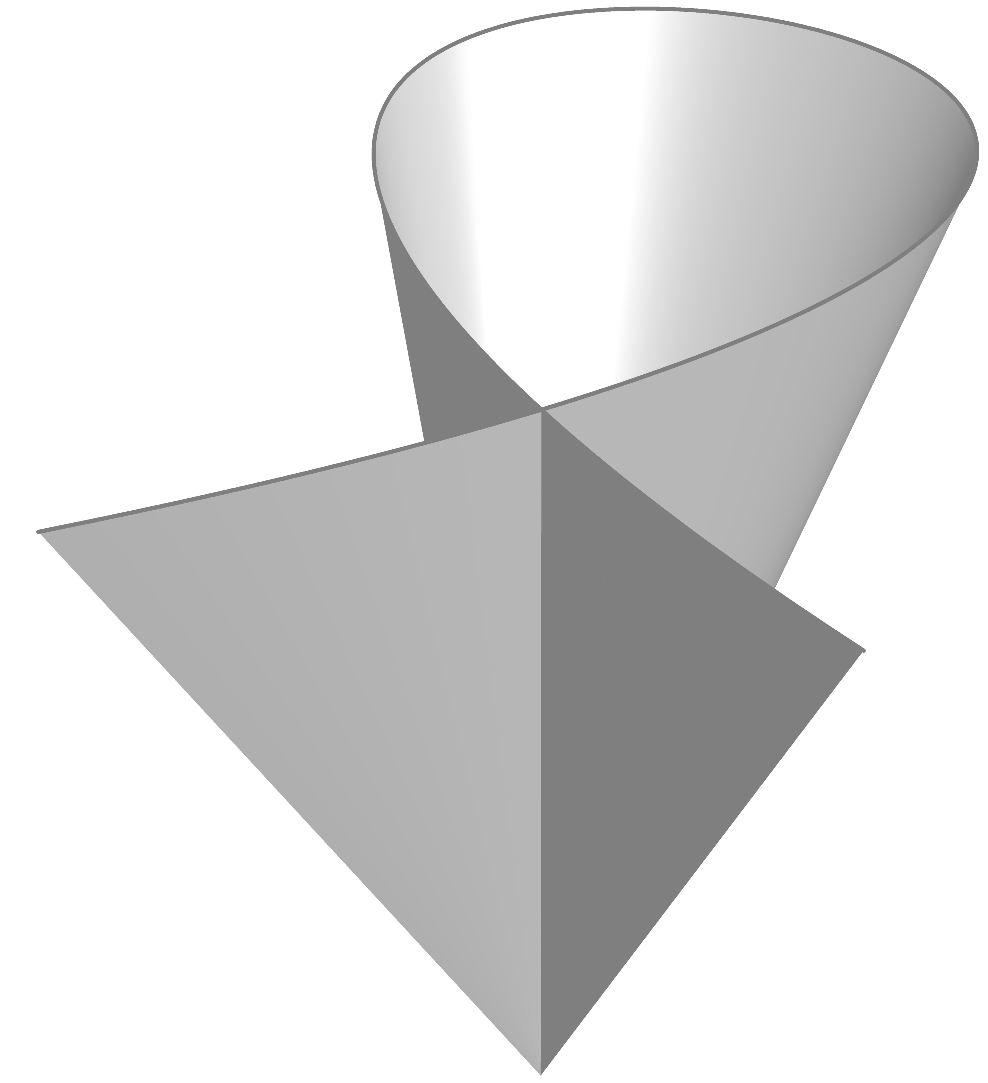
\includegraphics[width=4cm]{cone-over-cubic}
\end{center}

The recipe: given an algebraic equation, like \(y^2=x^2+x^3\):
\begin{enumerate}
\item 
Find the degree \(n\) of the highest term; in this example \(n=3\). 
\item
Invent a new variable \(z\).
\item
Multiply each term by a power of \(z\) so that the total degree of each term reaches \(n\).
\end{enumerate}
A polynomial is \emph{homogeneous}\define{homogeneous!polynomial}\define{polynomial!homogeneous} if all of its terms have the same total degree, i.e. sum of degrees in all variables.

\begin{problem}{projective.plane:homogenise}
Homogenise \(x^2y - x^2 + y = 1 + 2x - y^2x^3\).
\end{problem}


In sage:
\begin{sageblock}
R.<x,y,z> = PolynomialRing(QQ)
p = x^3+x*y+1
p.homogenize(z)
\end{sageblock}
yields \(\sage{p.homogenize(z)}\).

The homogenised polynomial equation \(y^2z = xz^2 + x^3\)  has all terms of degree 3, so if we rescale \(x,y,z\) to \(tx,ty,tz\), we rescale both sides of the equation by \(t^3\), so solutions \((x,y,z)\) rescaled remain solutions \((tx,ty,tz)\).
Thefore every solution lies on a line through the origin consisting of other solutions.
The set of solutions is a surface, which is a union of lines through the origin.
A \emph{projective plane curve}\define{projective!plane curve}\define{plane curve!projective}\define{curve!projective plane} is the set of lines through the origin satisfying a nonzero homogeneous polynomial.


\section{Conics}

\begin{example}
Take a hyperbola \(xy=1\) in the affine plane, 
\begin{center}
\documentclass[tikz]{standalone}
\usepackage{pgfplots}\pgfplotsset{compat=1.12}
\begin{document}
\pgfplotsset{every axis/.append style={
                    axis x line=middle,    % put the x axis in the middle
                    axis y line=middle,    % put the y axis in the middle
                    axis line style={<->,color=blue}, % arrows on the axis
                    xlabel={$x$},          % default put x on x-axis
                    ylabel={$y$},          % default put y on y-axis
            }}
\begin{tikzpicture}
    \begin{axis}[
            xmin=-8,xmax=4,
            ymin=-8,ymax=4,
            grid=both,
            ]
            \addplot [domain=-3:-0.01,samples=50]({x},{1/x}); 
            \addplot [domain=0.01:3,samples=50]({x},{1/x}); 
    \end{axis} 
\end{tikzpicture}
\end{document}

\end{center}
and homogenise to \(xy=z^2\), as we see from three different perspectives:
\begin{center}
\includegraphicsinexample[width=8cm]{cone-over-hyperbola-p0}
\includegraphicsinexample[width=8cm]{cone-over-hyperbola-p1}
\includegraphicsinexample[width=8cm]{cone-over-hyperbola-p2}
\end{center}
If we slice the surface along a plane like \(z=2\), parallel to the plane we drew but higher up, that plane \(z=2\) intersects our surface in a dilated hyperbola.
But if we slice the surface along the plane \(x=1\), we get \(xy=z^2\) to become \(y=z^2\), a parabola:
\includegraphicsinexample[width=8cm]{cone-over-parabola}
Suitable linear changes of variable interchange the \(x\) and \(z\) axes, so suitable projective automorphisms identify the two affine curves: the hyperbola and the parabola.
In particular, the two curves have isomorphic fields of rational functions.
They \emph{don't} have isomorphic rings of regular functions.

If instead we slice our surface with the plane \(x+y=1\),
\includegraphicsinexample[width=8cm]{cone-over-ellipse}
we get \(y=1-x\) plugged in to \(xy=z^2\), which simplifies to 
\[
\pr{x-\frac{1}{2}}^2 + z^2 = \frac{1}{4},
\]
a circle of radius \(\frac{1}{2}\).
So again the circle is birational to the parabola and to the hyperbola, and they all have the same rational function fields.
In these pictures we can see why the conics are called \emph{conics}: they are all slices of the same cone.
\end{example}

\begin{example}
The affine curve \(x^2+y^2=-1\) has no real points on it, but has complex points.
It homogenises to \(x^2+y^2+z^2=0\), a ``sphere of zero radius'', with the origin as its only real point, but with again many complex points.
The complex linear change of variables \(X=x-iy, Y=x+iy, Z=iz\) gives us \(XY=Z^2\), the same projective curve as before.
So these curves are all birational over the complex numbers, and indeed are all identified by automorphisms of the complex projective plane.
\end{example}

\begin{problem}{projective.plane:dehomogenise}
By the same trick of homogenising and dehomogenising in various variables, draw the same sort of pictures for the circle \(x^2+y^2=1\) to see what cone it homogenises to, and what curves it makes when you intersect that cone with the planes (a) \(x=1\), (b) \(y=1\) and (c) \(z=y+1\). 
\end{problem}

\section{Counting intersections of curves}

\epigraph[author={Chico Marx}]{Who are you going to believe, me or your own eyes?}\SubIndex{Marx, Chico}

\begin{example}
A line through a cubic curve
\begin{center}
\inputinexample{cubic-curve-4}
\end{center}
can hit as many as 3 points.
\end{example}
\begin{example}
Two conics
\begin{center}
\newcommand{\conicshift}{-.5}
\inputinexample{2-conics}
\end{center}
can intersect at as many as 4 points, but sometimes only at 3 points:
\begin{center}
\newcommand{\conicshift}{.875}
\inputinexample{2-conics}
\end{center}
\end{example}
\begin{example}
Some conics don't appear to intersect at all
\begin{center}
\newcommand{\conicshift}{4}
\inputinexample{2-conics}
\end{center}
but keep in mind that our points can have coordinates in the algebraic closure, so they actually intersect.
\end{example}
\begin{example}
The conics \(x^2+y^2=1\) and \((x-4)^2+y^2=1\):
\inputinexample{unnested-circles}
intersect at \((x,y)=(2,\pm i \sqrt{15})\). 
\end{example}
\begin{example}
Some conics appear not to have even complex intersections, such as \(x^2+y^2=1\) and \(x^2+y^2=2\).
\inputinexample{nested-circle}
But in the projective plane, we can homogenise to \(x^2+y^2=z^2\) and \(x^2+y^2=2z^2\), and then intersect with the plane \(x=1\), to get \(1+y^2=z^2\) and \(1+y^2=2z^2\), which intersect at \((y,z)=(\pm i,0)\).
\end{example}

\begin{problem}{projective.curves:find.the.points}
Find all points of the curve \(x^3+x^2y+xy^2+y^3+x^2=1\) which lie ``at infinity'', i.e. on the line \(z=0\) in homogeneous coordinates, over the field \(k=\C{}\).
\end{problem}
\begin{answer}{projective.curves:find.the.points}
Homogenize to \(x^3+x^2y+xy^2+y^3+x^2z=z^3\), and then set \(z=0\) to get the homogeneous equation \(x^3+x^2y+xy^2+y^3=0\).
Factor: \((x+y)(x^2+y^2)=0\).
So \(x+y=0\), i.e. \([x,-x,0]=[1,-1,0]\), or \(x^2+y^2=0\), which factors over any field \(k\) which contains an element \(i\) so that \(i^2=-1\), as \((x-iy)(x+iy)=0\), i.e. \(y=\pm ix\), so \([x,ix,0]=[1,i,0]\) and \([x,-ix,0]=[1,-i,0]\).
Hence the points of our curve that lie on the line at infinity are \([1,-1,0], [1,i,0], [1,-i,0]\).
\end{answer}

\begin{problem}{projective.curves:find.the.points.5}
Find all points of the curve \(y^2+y=x^3+x+1\) on the projective plane over the field \(k=\Z{}/5\Z{}\).
\end{problem}
\begin{answer}{projective.curves:find.the.points.5}
Start with the affine plane.
Remember (from problem~\vref{problem:polynomials:quadratic.formula}) that you can use the quadratic formula:
\[
y=\frac{-1\pm\sqrt{1-4(-x^3-x-1)}}{2}.
\]
Simplify, using \(2^{-1}=3\) and \(4=-1\), to:
\[
y=3(-1\pm\sqrt{-x^3-x})
\]
Note that \(0^2=0, 1^2=1, 2^2=4, 3^2=9=4, 4^2=16=1\), so only \(0,1,4\) have square roots.
\begin{itemize}
\item
\(x=0\): \(-x^3-x=0\), \(y=-3=2\), \([x,y,z]=[0,2,1]\).
\item
\(x=1\): \(-x^3-x=3\), no square root of \(3\), no solution.
\item
\(x=2\): \(-x^3-x=-8-2=0\), \(y=-3=2\), \([x,y,z]=[2,2,1]\).
\item
\(x=3\): \(-x^3-x=-27-3=0\), \(y=-3=2\), \([x,y,z]=[3,2,1]\).
\item
\(x=4\): \(-x^3-x=-68=2\), no square root of \(2\) no solution.
\end{itemize}
We still need the points ``at infinity''.
Homogenize: \(y^2z+yz^2=x^3+xz^2+z^3\), and set \(z=0\): \(0=x^3\), so \(x=0\), i.e. \([x,y,z]=[0,y,0]\), and rescale \(y\) to \([0,1,0]\).
Final answer: \([0,2,1], [2,2,1], [3,2,1], [0,1,0]\).
\end{answer}



\begin{lemma}\label{lemma:finitely.many.lines}
Suppose that \(k\) is an infinite field.
Then for any finite set of lines in \(\Proj[2]{k}\), there are infinitely many points of \(\Proj[2]{k}\) not on any of those lines.
\end{lemma}
\begin{proof}
If we work in the affine plane, the points \((x,y)\) lying on those lines must satisfy one of the associated linear equations, say \(y=m_i x + b_i\) or \(x=c_i\).
Pick a number \(x_0\) not among the constants \(c_i\).
Now we have finitely many values \(y=m_i x_0 + b_i\) to avoid; pick \(y\) to not be one of those.
\end{proof}


\begin{lemma}\label{lemma:one.variable.splits}
Every nonzero homogeneous polynomial of degree \(n\) in two variables over a field \(k\) has \(n\) roots, counted with multiplicities, in \(\Proj[1]{\bar{k}}\), and so splits into a product of homogeneous linear factors over \(\bar{k}\).
\end{lemma}
\begin{proof}
As part of the proof, we define multiplicities of zeroes of a homogeneous polynomial \(p(x,y)\) to be multiplicities of linear factors.
So we are saying precisely that \(p(x,y)\) factors into \(n\) linear factors.
If \(p(x,y)\) has a linear factor, divide it out and apply induction.
Since \(y\) is not a linear factor of \(p(x,y)\), \(p(x,1)\) has degree \(n\), say \(p(x,1)=a(x-x_1)\dots(x-x_n)\).
The homogeneous polynomial
\[
r(x,y) \defeq p(x,y)-a(x-x_1y)(x-x_2y)\dots(x-x_ny)
\]
vanishes at \(y=1\) for any \(x\), so by homogeneity vanishes for any \(y \ne 0\).
Fixing any value of \(x\), there are infinitely many values of \(y\) at which \(0=r(x,y)\), and so \(r(x,y)\) vanishes everywhere.
\end{proof}

\begin{example}
The polynomial 
\[
p(x,y)=x^3+x^2y-2xy^2
\]
becomes 
\[
p(x,1)=x^3+x^2-2x=x(x-1)(x+2),
\]
so that 
\[
p(x,y)=x(x-y)(x+2y).
\]
\end{example}
\begin{example}
The family of curves with \(y^2=ax\) contains the curve \(y^2=0\) when \(a=0\), a line.
So a family of curves of degree 2 contains a curve of degree 1.
It is natural to think of the curve being a ``double line'' when \(a=0\).
\end{example}

Similarly, we can say that a \emph{multiple component}\define{component!multiple} of a curve means a curve given by an equation which is a positive integer power of an irreducible homogeneous polynomial, say \(0=f(x,y,z)^k\) giving a component with multiplicity \(k\).
From now on, we allow projective plane curves to have components with positive integer multiplicities.





\section{Breaking curves into components}


\begin{theorem}[Study]\define{theorem!Study}\define{Study!theorem}\label{theorem:Study}
Every algebraic curve in the projective plane has a unique decomposition into irreducible algebraic curves, its \emph{components}.
To be more precise, every nonzero homogeneous polynomial in 3 variables \(f(x,y,z)\) has a decomposition
\[
f=a_0 g_1^{k_1} g_2^{k_2} \dots g_n^{k_n},
\]
into a product of a nonzero constant \(a_0\) and several coprime irreducible homogeneous polynomials \(g_j(x,y,z)\) to various positive integer powers, unique up to rescaling the constant and the polynomials by nonzero constants.
\end{theorem}
\begin{proof}
Suppose that \(g\) is an irreducible polynomial and that \(f=0\) at every point in \(\bar{k}\) where \(g=0\). 
We want to prove that \(g\) divides \(f\).
Work in the affine plane \(z=1\).
Think of each equation as a polynomial in one variable \(x\), but with coefficients rational functions of \(y\).
By corollary~\vref{corollary:resultant.effective}, after perhaps a linear change of variables, the resultant in \(y\) vanishes just at those \(x\) values where there are simultaneous roots.
In particular, the number of different values of \(x\) where such roots occur is never more than the degree of the resultant, as a polynomial in \(x\).
For each value \(x=c\) (over \(\bar{k}\)) for which \(g(c,y)\) is not constant, the values of \(y\) at which \(g(c,y)=0\) also satisfy \(f(c,y)=0\), so the resultant vanishes.
Therefore this resultant is the zero polynomial.
If the curve where \(f=0\) is the union of distinct irreducible curves given by equations \(g_i=0\), then each of these \(g_i\) divides \(f\), so their product divides \(f\).
Apply induction on the degree of \(f\).
\end{proof}

\begin{theorem}
Every rational morphism of projective plane algebraic curves \(f \colon B \to C\) is constant or onto a finite union of components of \(C\), at most one for each component of \(B\).
\end{theorem}
\begin{proof}
We can assume that \(B\) is irreducible, and we have already assumed that our field is algebraically closed by definition of the points of the curve.
Our rational morphism is
\[
f(x,y,z)=(p(x,y,z),q(x,y,z),r(x,y,z)).
\]
If \(B=(b(x,y,z)=0)\) then the system of equations
\[
 b(a,b,c)=0, a=a(x,y,z), b=b(x,y,z), c=c(x,y,z)
\]
has (after perhaps a linear change of \(x,y,z\) variables) resultant
eliminating \(x,y,z\) given by some algebraic equation in \(a,b,c\) which specifies which points lie in the image.
By corollary~\vref{corollary:resultant.effective} this equation is not trivial.
Split \(C\) into irreducibles \(C_1, C_2, \dots, C_N\), say \(C_j=\pr{c_j=0}\). 
Then \(c_1 c_2 \cdots c_N \circ f=0\) on \(B\), since \(f\) takes \(B\) to \(C\).
So if \(B=\pr{b(x,y,z)=0}\) then \(b\) is divisible by \(c_1 c_2 \cdots c_N \circ f\) in any affine chart.
If \(c_1 \circ f\) is not zero on \(B\) then divide by it to see that already  \(c_2 \cdots c_N \circ f=0\) on \(B\).
So \(f\) takes \(B\) into \(C_2 \cup \dots \cup C_N\).
We can assume that \(c_j \circ f = 0\) on \(B\) for every \(j\), i.e. that \(B \subset f^{-1}C_j\) for every \(j\), i.e. that 
\[
f(B) \subset \bigcap_j C_j:
\]
there is only one such \(C_j\), i.e. \(C\) is irreducible.
Hence the image is precisely \(C\).
\end{proof}


\section{Counting intersections}

A triangle \(pqr\) is \emph{generic}\define{generic!triangle}\define{triangle!generic} for two algebraic projective plane curves \(B, C\) if 
\begin{enumerate}
\item
neither curve passes through \(q\) and
\item 
no line connecting two intersection points of \(B\) and \(C\) lies through \(q\).
\end{enumerate}
\begin{center}
\documentclass[tikz]{standalone}
\usetikzlibrary{intersections}
\usepackage{xparse}
\colorlet{curveZero}{gray!75}
\colorlet{curveOne}{blue!60}
\colorlet{curveTwo}{brown!50!gray}
\colorlet{curveThree}{green!40!gray}
\colorlet{curveFour}{red!50!gray}
\NewDocumentCommand\DrawDotInPlot{O{}mmO{}}%
{%
\fill[gray!20,draw=gray] (axis cs:{#2},{#3}) circle (1.3pt) node[above,black,#4] {\(#1\)};%
}%
\NewDocumentCommand\DrawDot{O{}mmO{}}%
{%
\fill[gray!20,draw=gray] ({#2},{#3}) circle (1.3pt) node[above,black,#4] {\(#1\)};%
}%
\NewDocumentCommand\DrawNode{O{}m}%
{%
\fill[gray!20,draw=gray] (#2) circle (1.3pt) node[above,black] {\(#1\)};%
}%
\colorlet{axisColor}{gray!50}
\tikzstyle{shapeZero}=[fill=curveZero,opacity=.4]
\tikzstyle{shapeOne}=[fill=curveOne,opacity=.4]
\tikzstyle{shapeTwo}=[fill=curveTwo,opacity=.4]
\tikzstyle{shapeThree}=[fill=curveThree,opacity=.4]
\tikzstyle{groupElementLabel}=[minimum size=2.4em]
\tikzstyle{groupElement}=[minimum size=2.4em,shapeZero,draw=curveZero]
\tikzstyle{cosetOne}=[minimum size=2.4em,shapeOne,draw=curveOne]
\tikzstyle{cosetTwo}=[minimum size=2.4em,shapeTwo,draw=curveTwo]


\begin{document}
\begin{tikzpicture}[scale=3]
\draw[curveZero,very thick] 
({cos(90)},{sin(90)}) node[black,above] {\(q\)} -- 
({cos(90+120)},{sin(90+120)}) node[black,below left] {\(p\)} -- 
({cos(90+2*120)},{sin(90+2*120)}) node[black,below right] {\(r\)} -- cycle;
\draw[curveOne,name path=Bellipse,very thick] ({.5*cos(90)+.5*cos(90+2*120)},{.5*sin(90)+.5*sin(90+2*120)}) arc (30:390:.45);
\draw[curveTwo,name path=Cellipse,very thick] ({.5*cos(90)+.5*cos(90+2*120)},{.5*sin(90)+.5*sin(90+2*120)}) arc (30:390:.3 and .6);
\draw [axisColor, name intersections={of=Bellipse and Cellipse}]
(intersection-1) -- ({cos(90)},{sin(90)}) 
(intersection-2) -- ({cos(90)},{sin(90)}) 
(intersection-3) -- ({cos(90)},{sin(90)}) 
(intersection-4) -- ({cos(90)},{sin(90)}); 
\end{tikzpicture}
\end{document}

\end{center}
A triangle \(pqr\) is \emph{very generic}\define{very generic!triangle}\define{triangle!very generic}
\define{generic!triangle!very} for curves \(B\) and \(C\) if it is generic and there is no intersection point of \(B\) and \(C\) along the line \(qr\).
Keep in mind that we allow intersection points, and points of the triangle, to have coordinates in the algebraic closure of our field.
\begin{center}
\documentclass[tikz]{standalone}
\usetikzlibrary{intersections}
\usepackage{xparse}
\colorlet{curveZero}{gray!75}
\colorlet{curveOne}{blue!60}
\colorlet{curveTwo}{brown!50!gray}
\colorlet{curveThree}{green!40!gray}
\colorlet{curveFour}{red!50!gray}
\NewDocumentCommand\DrawDotInPlot{O{}mmO{}}%
{%
\fill[gray!20,draw=gray] (axis cs:{#2},{#3}) circle (1.3pt) node[above,black,#4] {\(#1\)};%
}%
\NewDocumentCommand\DrawDot{O{}mmO{}}%
{%
\fill[gray!20,draw=gray] ({#2},{#3}) circle (1.3pt) node[above,black,#4] {\(#1\)};%
}%
\NewDocumentCommand\DrawNode{O{}m}%
{%
\fill[gray!20,draw=gray] (#2) circle (1.3pt) node[above,black] {\(#1\)};%
}%
\colorlet{axisColor}{gray!50}
\tikzstyle{shapeZero}=[fill=curveZero,opacity=.4]
\tikzstyle{shapeOne}=[fill=curveOne,opacity=.4]
\tikzstyle{shapeTwo}=[fill=curveTwo,opacity=.4]
\tikzstyle{shapeThree}=[fill=curveThree,opacity=.4]
\tikzstyle{groupElementLabel}=[minimum size=2.4em]
\tikzstyle{groupElement}=[minimum size=2.4em,shapeZero,draw=curveZero]
\tikzstyle{cosetOne}=[minimum size=2.4em,shapeOne,draw=curveOne]
\tikzstyle{cosetTwo}=[minimum size=2.4em,shapeTwo,draw=curveTwo]


\begin{document}
\begin{tikzpicture}[scale=3]
\draw[curveZero,very thick] 
({cos(90)},{sin(90)}) -- 
({cos(90+120)},{sin(90+120)}) -- 
({2*cos(90+2*120)},{sin(90+2*120)}) -- cycle;
\draw[curveOne,very thick,name path=Bellipse] ({.5*cos(90)+.5*cos(90+2*120)},{.5*sin(90)+.5*sin(90+2*120)}) arc (30:390:.45);
\draw[curveTwo,very thick,name path=Cellipse] ({.5*cos(90)+.5*cos(90+2*120)},{.5*sin(90)+.5*sin(90+2*120)}) arc (30:390:.3 and .6);
\draw [axisColor, name intersections={of=Bellipse and Cellipse}]
(intersection-1) -- ({cos(90)},{sin(90)}) 
(intersection-2) -- ({cos(90)},{sin(90)}) 
(intersection-3) -- ({cos(90)},{sin(90)}) 
(intersection-4) -- ({cos(90)},{sin(90)}); 
\end{tikzpicture}
\end{document}

\end{center}

By projective automorphism, we can make any triangle become the one whose vertices are \[[0,0,1],[1,0,0],[0,1,0].\]
This projective automorphism is unique up to rescaling the variables.
In the affine plane, these vertices are the points \((0,0), (\infty,0), (0,\infty)\).
Suppose that our two curves have equations \(B=(b(x,y)=0)\) and \(C=(c(x,y)=0)\).
The triangle is generic just when 
\begin{enumerate}
\item
\((0,\infty)=[0:1:0]\) is not on \(B\) or \(C\), and
\item
no vertical line intersects two intersection points of \(B\) and \(C\).
\end{enumerate}
In a more algebraic description:
\begin{enumerate}
\item
\(b(x,y)\) and \(c(x,y)\) both have nonzero constants in front of their highest terms in \(y\) and
\item
for any constant \(x=x_0\), \(b(x_0,y)\) and \(c(x_0,y)\) have at most one common root in \(y\).
\end{enumerate}
If the triangle is generic, it is also very generic just when there is no zero of the homogeneous polynomials \(b(x,y,z)\), \(c(x,y,z)\) on the line at infinity, i.e. the line \(z=0\), or, in other words, the highest order terms of \(b(x,y)\) and \(c(x,y)\) (which are homogeneous of the same degree as \(b(x,y)\) and \(c(x,y)\)) have no common root on \(\Proj{1}\).
The resultant \(\resultant{b}{c}(x)\) in \(y\) depends, up to constant factor, only on the choice of curves \(B\) and \(C\) and the choice of triangle.
The \emph{intersection number}\define{intersection number} of \(B\) and \(C\) at a point \(p=(x,y)\), denoted 
\(\multiplicity{p}{B}{C}\),\Notation{BCp}{\multiplicity{p}{B}{C}}{multiplicity of intersection of curves \(B\) and \(C\) at point \(p\)} is the multiplicity of \(x\) as a zero of \(\resultant{b}{c}(x)\).
If \(p\) is not a point of both \(B\) and \(C\) then define
\(\multiplicity{p}{B}{C}\defeq 0\).
If \(p\) lies on a common component of \(B\) and \(C\) then let \(\multiplicity{p}{B}{C}\defeq\infty\).
Danger: so far, the intersection number depends on the choice of triangle.
Let \(\intersectionnumber{B}{C}\defeq \sum_p \multiplicity{p}{B}{C}\)\Notation{\#BC}{\intersectionnumber{B}{C}}{total multiplicity of intersection of curves \(B\) and \(C\)} summed over all points \(p\).

\begin{example}
Let \(b(x,y)\defeq y+x\) and \(c(x,y)\defeq y\). 
The intersection points of the lines \((b(x,y)=0)\) and \((c(x,y=0)\) in the affine plane are at \(0=y=y+x\), i.e. at the origin.
In the projective plane, there is no further intersection point, as the equations are already homogeneous.
So the standard triangle is very generic for these two lines.
The resultant of \(b(x,y), c(x,y)\) in \(y\) is \(r(x)=x\).
So the two lines \(B=(y+x=0)\) and \(C=(y=0)\) have \(\multiplicity{(0,0)}{B}{C}=1\).
Similarly any two lines have intersection number 1 at their intersection point.
\end{example}
\begin{example}
Let \(B\defeq (xy^2+y=0)\) and \(C\defeq (xy^2+y+1=0)\).
The curves intersect in the affine plane at 
\[
(x,y)=\pr{-2,-\frac{1}{2}}
\]
(assuming that \(2 \ne 0\) in our field).
Homogenize to find also the intersection point \((0,\infty)=[0:1:0]\).
So the coordinate triangle is not generic.
As previously, if we change \(x\) to \(x+\lambda\) for any constant \(\lambda \ne 0\), our curves change to
\[
B=(\lambda y^3+xy^2+y=0), C=(2\lambda y^3+2xy^2+y+1).
\]
They now intersect at
\[
(x,y)=(-1-\lambda,1)=[-1-\lambda,1,1].
\]
(We previously saw this from looking at the resultant \(r(x)=-\lambda^2(\lambda+1+x)\).)
After homogenizing and then setting \(y=1\), we also find another intersection at \([x,y,z]=[-\lambda,1,0]\).
The standard triangle is generic for these curves, since the two intersection points lie on different lines through \([0,1,0]\).
But it is not very generic, because our second intersection point lies outside the affine plane, on the line at infinity.
We can only calculate the intersection number at the first point, where the resultant vanishes to degree \(1\), so an intersection number
\[
\multiplicity{(-\lambda-1,1)}{B}{C}=1.
\]
The other point is not in the affine plane, so intersection multiplicity is not defined at that point, at least by our definition.
\end{example}

\begin{theorem}[B\'ezout]\label{theorem:baby.B\'ezout}\define{theorem!B\'ezout}\define{B\'ezout!theorem}
Over any field, take two projective algebraic plane curves \(B\) and \(C\) not sharing a common component.
Over some finite degree extension of the field there is a very generic triangle for the curves.
For any generic triangle, \(\intersectionnumber{B}{C} \le \degree{B}\degree{C}\).
A generic triangle is very generic just when equality holds.
\end{theorem}
\begin{proof}
Split \(B\) and \(C\) into irreducibles and add up intersections by multiplying resultants: without loss of generality we can assume that \(B\) and \(C\) are irreducible.

By proposition~\vref{proposition:resultant.degree}, there are at most \(\degree{B}\degree{C}\) values of \(x\) that occur on intersection points, and by the same reasoning at most that number of \(y\) values, so finitely many intersection points.

Since there are finitely many intersection points, there are finitely many lines through them. 
By lemma~\vref{lemma:finitely.many.lines} we can pick one vertex of our triangle to avoid lying on any of them (after perhaps replacing by an extension field), while arbitrarily picking the other two vertices to be any two distinct points.
So we have a generic triangle, and we can assume that its vertices are \((0,0)\), \((\infty,0)\) and \((0,\infty)\).
We can then move the line at infinity to avoid the intersection points (again in some extension field), so there is a very generic triangle.

Pick any generic triangle.
No two intersection points lie on any line through \((0,\infty)\), i.e. on any vertical line: all of the intersection points have distinct \(x\) values.
There is no intersection point at \((0,\infty)\), i.e. the highest order terms in \(y\) in the equations have no common zero.
Therefore even when \(b(a,y)\) drops degree at some value of \(x=a\), \(c(a,y)\) doesn't, so the resultant is the product of the values of \(b(a,y)\) at the roots \(y\) of \(c(a,y)\), vanishing precisely at the values of \(x\) where the curves have an intersection.
In the proof of proposition~\vref{proposition:resultant.degree}, we found the degree of the resultant to be at most \(\degree{b}\degree{c}\) and nonzero.
There are at most a number of intersection points given by the degree of the resultant as a polynomial.
Hence the sum of the intersection numbers over the intersections in the affine plane is the sum of the degree of root over all roots of the resultant, so at most the degree of the resultant.
Our triangle is very generic just when this sum covers all intersection points, as there are none on the line at infinity.

We still need to see that for our very generic triangle, the degree of the resultant is precisely \(\degree{B}\degree{C}\).
The assumption of being very generic is expressed algebraically as saying that the homogeneous polynomials \(b(x,y,z), c(x,y,z)\) have no common roots along \(z=0\).
In other words, \(b(x,y,0)\) and \(c(x,y,0)\) have no common roots on \(\Proj{1}\).
So the resultant of \(b(x,y,0),c(x,y,0)\) in \(y\) is nonzero, and has degree \(\degree{B}\degree{C}\).
But the degree of resultant of \(b(x,y,z), c(x,y,z)\) can be no less for variable \(z\) as for the fixed value \(z=0\).
Therefore the resultant has the required degree.
\end{proof}



\begin{theorem}\label{theorem:intersection.number.definition}
To any two projective algebraic plane curves \(B\) and \(C\) over a field \(k\) and any point \(p\) of the projective plane defined over the algebraic closure \(\bar{k}\) of \(k\), there is a unique quantity \(\multiplicity{p}{B}{C}\) so that
\begin{enumerate}
\item\label{item:B\'ezout.first}
\(\multiplicity{p}{B}{C} = \multiplicity{p}{C}{B}\) and
\item
\(\multiplicity{p}{B}{C}=0\) just when \(p\) does not lie on any common point of \(B\) and \(C\) defined over \(\bar{k}\) and
\item
\(\multiplicity{p}{B}{C}=\infty\) just when \(p\) lies on a common component of \(B\) and \(C\) defined over \(\bar{k}\) and
\item
\(\multiplicity{p}{B}{C}\) is a positive integer otherwise and
\item
two distinct lines meet with intersection multiplicity 1 at their unique point of intersection and
\item
if \(B\) splits into components (perhaps with multiplicities) \(B_1\) and \(B_2\), then \(\multiplicity{p}{B}{C}=\multiplicity{p}{B_1}{C}+\multiplicity{p}{B_2}{C}\) and
\item\label{item:B\'ezout.last}
if \(B\) and \(C\) are defined by homogeneous polynomials \(b(x,y,z)\) and \(c(x,y,z)\) and \(E\) is the curve defined by \(bh+c\) where \(h(x,y,z)\) has degree \(\degree{h}=\degree{b}-\degree{c}\), then \(\multiplicity{p}{B}{C}=\multiplicity{p}{B}{E}\).
\end{enumerate}
Moreover, \(\multiplicity{p}{B}{C}\) can be computed as defined above using any generic triangle.
\end{theorem}
\begin{proof}
In this proof, we write \(\multiplicity{p}{b}{c}\) instead of \(\multiplicity{p}{B}{C}\) if \(B\) is cut out by the equation \(0=b(x,y,z)\) and \(C\) by \(0=c(x,y,z)\).
First we prove that the conditions \ref{item:B\'ezout.first}--\ref{item:B\'ezout.last} determine the multiplicity uniquely.
Since they are independent of choice of affine chart, this ensures that the multiplicity is also independent.
We then check that our definition above satisfies these, so must be determined by these conditions independent of the choice of affine chart made in the definition above.

Any two notions of multiplicity agree on common components of \(B\) and \(C\), and on points not belonging to \(B\) or \(C\), by the conditions above.
So we only need to check points of positive finite multiplicity.
We can assume by induction that \(B\) and \(C\) are both irreducible, and cut out by irreducible homogeneous polynomials \(b\) and \(c\).
Suppose that we have two different methods of calculating an intersection number satisfying our various conditions, one of which we can take to be the definition by the resultant above.
By induction suppose that they agree wherever they both assign a value less than the larger of the two values that they assign as \(\multiplicity{p}{b}{c}\).

Take affine coordinates in which \(p=(0,0)\).
If \(\degree{b}(x,0)=0\) then \(b(x,0)=0\) so \(b(x,y)\) is divisible by \(y\), not irreducible, so our result holds by induction.
The same holds if \(\degree{c}(x,0)=0\).
So both \(b\) and \(c\) have positive degree in each of \(x\) and \(y\) when the other variable is set to zero.
Rescale to get both to have unit coefficient in \(x\):
\begin{align*}
b(x,y) &= x^{\beta} + \dots , \\
c(x,y) &= x^{\gamma} + \dots.
\end{align*}
Suppose (after perhaps swapping the names of \(b\) and \(c\)) that \(\beta \le \gamma\) and let
\[
h(x,y)
\defeq 
c(x,y)-x^{\gamma-\beta}b(x,y).
\]
By construction, \(h(x,0)\) has degree in \(x\) at most \(\gamma-1\).
Our last property of intersection multiplicity above demands that \(\multiplicity{p}{b}{c}=\multiplicity{p}{b}{h}\).
Therefore we can replace \(c\) by \(h\) and repeat, lowering the degree in \(x\) by induction.
This proves uniqueness of intersection multiplicities satisfying our axioms.

We want to prove existence, i.e. that the recipe we defined above satisfies our axioms above.
\begin{enumerate}
\item
Resultants change sign when we swap polynomials, so \(\resultant{b}{c}=-\resultant{c}{b}\).
\item
Follows from theorem~\vref{theorem:baby.B\'ezout}.
\item
Follows from theorem~\vref{theorem:baby.B\'ezout}.
\item
Follows from theorem~\vref{theorem:baby.B\'ezout}.
\item
Follows by direct computation of the resultant.
\item
Follows from lemma~\vref{lemma:resultants.multiply}. 
\item
Follows from proposition~\vref{proposition:factored.resultants}, and the existence of splitting fields.
\end{enumerate}
\end{proof}

We restate B\'ezout's theorem without reference to generic triangles, since the previous theorem proves that they are irrelevant.
\begin{theorem}
[B\'ezout]\label{theorem:B\'ezout}\define{theorem!B\'ezout}\define{B\'ezout!theorem}
Over any field \(k\), take two projective algebraic plane curves \(B\) and \(C\) not sharing a common component.
Over the algebraic closure \(\bar{k}\) of the field, the intersection numbers of the intersection points sum to
\[
\sum_{p \in \Proj[2]{\bar{k}}} \multiplicity{p}{B}{C} = \degree{B}\degree{C}.
\]
\end{theorem}


\section{Sage}

Pieter Belmans wrote the following sage code to find the intersection number of two algebraic curves at a point.
First we find the minimum degree of any term in a polynomial \(f(x)\) of one variable.
\begin{sageblock}
def ldegree(f):
    minimum = infinity
    for (n, m) in f.dict():
        minimum = min(minimum, n)
    return minimum
\end{sageblock}
Given any two polynomials \(b, c\) in two variables, we want to figure out what the two variables are:
\begin{sageblock}
def determine_variables(b, c):
    if len(b.variables()) == 2:
        return b.variables()
    if len(c.variables()) == 2:
        return c.variables()
    if len(b.variables()) == len(c.variables()) == 1:
        if b.variables() == c.variables():
            return (b.variable(0), 0)
        else:
            return (c.variable(0), b.variable(0))
    return (0,0)
\end{sageblock}
Finally, we use our definition of intersection number, and induction, to compute intersection numbers recursively.
\begin{sageblock}
def intersection_number(b, c, point = (0,0)):
    (x,y) = determine_variables(b, c)
    # translate both curves to origin and calculate it there
    b = b.subs({x:x + point[0], y:y + point[1]})
    c = c.subs({x:x + point[0], y:y + point[1]})
    # if $b(0,0)\neq 0$ or $c(0,0)\neq 0$ they don't intersect in the origin
    if b.subs({x:0, y:0}) != 0 or c.subs({x:0, y:0}) != 0: 
        return 0
    # if $b$ or $c$ are zero they don't intersect properly
    if b == 0 or c == 0: 
        return Infinity
    # we only look at factors of $x$
    f = b.subs({y:0})
    g = c.subs({y:0})
    # $b$ contains a component $y=0$
    if f == 0:
        # $c$ contains a component $y=0$ too, no proper intersection
        if c == 0: 
            return infinity
        # remove common $y^n$ in $b$, count degree of $x$ in $c$ and recurse
        else:
            f = b.quo_rem(y)[0]
            return ldegree(g) + intersection_number(f, c)
    # $b$ does not contain a component $y=0$
    else:
        # $c$ *does* contain a component $y=0$
        if g == 0:
            g = c.quo_rem(y)[0]
            return ldegree(f) + intersection_number(b, g)
        # we recurse by removing factors of $x$
        else:
            p, q = f.lc(), g.lc()
            r, s = f.degree(), g.degree()
            # we drop the highest degree term
            if r <= s:
                return intersection_number(b, p*c - q*x^(s-r)*b)
            else:
                return intersection_number(q*b - p*x^(r-s)*c, c)
\end{sageblock}
A test run:
\begin{sageblock}
P.<x,y> = PolynomialRing(QQ)
b = P(x^2+y^2)^2+3*x^2*y-y^3
c = P(x^2+y^2)^3-4*x^2*y^2
intersection_number(b,c)
\end{sageblock}
yields \(\sage{intersection_number(b,c)}\), the intersection number at the origin of the curves:
\begin{center}
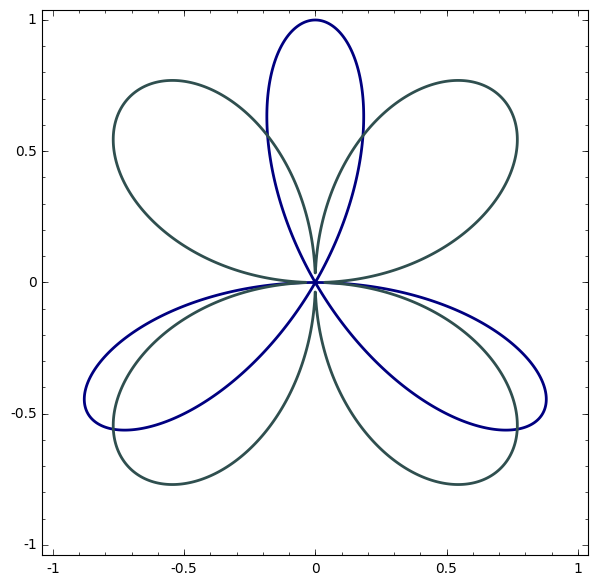
\includegraphics[width=6cm]{curve_intersection}
\end{center}
%p=implicit_plot(b, (x,-1, 1), (y,-1, 1),color="navy",linewidth=2, plot_points=1500)
%q=implicit_plot(c, (x,-1, 1), (y,-1, 1),color="darkslategray",linewidth=2, plot_points=1500)
%show(p+q)

\chapter{Families of plane curves}

\epigraph[author={Leo Tolstoy}, source={Anna Karenina}]{All happy families are alike; each unhappy family is unhappy in its own way.}\SubIndex{Tolstoy, Leo}\SubIndex{Karenina, Anna}
 
 
 
 
 
 
 
\section{Pencils of curves}

Every curve \(C\) of degree \(n\) has a homogeneous equation \(c(x,y,z)=0\) of degree \(n\), unique up to rescaling, by Study's theorem (theorem~\vref{theorem:Study}).
Take two curves \(B\) and \(C\) of the same degree \(n\), with equations \(b(x,y,z)=0\) and \(c(x,y,z)=0\).
The level sets 
\[
\frac{b(x,y,z)}{c(x,y,z)} = r
\]
of the ratio form a collection of curves \(C_r\), called the \emph{pencil}\define{pencil} of curves containing \(B\) and \(C\).
The curve \(B\) is \(C_0\) while \(C\) is \(C_{\infty}\).
Every point \([x,y,z]\) in the plane lies on a unique one of these curves, with value \(r\) given by taking the value of \(p(x,y,z)/q(x,y,z)\) at that point, except for the points in \(B \cap C\), for which the ratio is never defined.
To be more precise, each curve \(C_r\) can also be written as
\[
p(x,y,z) = r q(x,y,z),
\]
(except for \(C_{\infty}=C\)).
The points of \(B \cap C\) belong to \emph{all} curves \(C_r\) of the pencil.
Moreover the degree of \(C_r\) is the same as that of \(B\) and \(C\).

\begin{example}
The lines through a point form a pencil: if \(B=(x=0)\) and \(C=(y=0)\) then \(C_r =(x=ry)\).
\begin{center}
\documentclass[11pt]{standalone}
\usepackage{xparse}
\usepackage{tikz}
\colorlet{curveZero}{gray!75}
\colorlet{curveOne}{blue!60}
\colorlet{curveTwo}{brown!50!gray}
\colorlet{curveThree}{green!40!gray}
\colorlet{curveFour}{red!50!gray}
\NewDocumentCommand\DrawDotInPlot{O{}mmO{}}%
{%
\fill[gray!20,draw=gray] (axis cs:{#2},{#3}) circle (1.3pt) node[above,black,#4] {\(#1\)};%
}%
\NewDocumentCommand\DrawDot{O{}mmO{}}%
{%
\fill[gray!20,draw=gray] ({#2},{#3}) circle (1.3pt) node[above,black,#4] {\(#1\)};%
}%
\NewDocumentCommand\DrawNode{O{}m}%
{%
\fill[gray!20,draw=gray] (#2) circle (1.3pt) node[above,black] {\(#1\)};%
}%
\colorlet{axisColor}{gray!50}
\tikzstyle{shapeZero}=[fill=curveZero,opacity=.4]
\tikzstyle{shapeOne}=[fill=curveOne,opacity=.4]
\tikzstyle{shapeTwo}=[fill=curveTwo,opacity=.4]
\tikzstyle{shapeThree}=[fill=curveThree,opacity=.4]
\tikzstyle{groupElementLabel}=[minimum size=2.4em]
\tikzstyle{groupElement}=[minimum size=2.4em,shapeZero,draw=curveZero]
\tikzstyle{cosetOne}=[minimum size=2.4em,shapeOne,draw=curveOne]
\tikzstyle{cosetTwo}=[minimum size=2.4em,shapeTwo,draw=curveTwo]


\begin{document}
\begin{tikzpicture}
\newcommand{\RRR}{1.8}
\foreach \i in {0,...,9}
{
\draw[axisColor] 
		({\RRR*cos(3.1415*\i/10 r)},{\RRR*sin(3.1415*\i/10 r)}) 
	-- ({-\RRR*cos(3.1415*\i/10 r)},{-\RRR*sin(3.1415*\i/10 r)});
}
\DrawDot{0}{0}
\end{tikzpicture}
\end{document}

\end{center}
\end{example}
\begin{example}
The pencil of conics containing the circle \(x^2+y^2=1\) and the reducible conic \(x^2=y^2\) (which is a pair of lines \(x=\pm y\)):
\[
\includegraphics[width=4cm]{pencils/pencil-1}
\]
Look at the 4 points where the circle intersects the two lines; these points lie in every conic in the pencil.
\end{example}
\begin{example}
The pencil of cubics containing \(y^2=x+x^3\) and \(xy^2=0\):
\[
\includegraphics[width=4cm]{pencils/pencil-2}
\]
\end{example}
\begin{example}
\emph{Danger}: for some values of \(r\), \(C_r\) might actually be of lower order than \(B\) or \(C\).
For example, if \(B=(y^2=x)\) and \(C=(-y^2=x)\), two conics, the pencil has curves \(C_r\) with equation
\[
\pr{1-r}y^2=(1+r)x,
\]
which drops order at \(r=1\), i.e. \(C_1\) is a line.
But note that if we homogenize,
\[
\pr{1-r}y^2=(1+r)zx,
\]
the curve \(C_1\) is actually a pair of lines.
In a pencil \(C_r\) for which \(C_0\) and \(C_{\infty}\) are irreducible, we rarely but occasional find reducible curves, as in this example, and we might picture that the moving curve \(C_r\) ``bubbles'' into reducible components.
\begin{center}
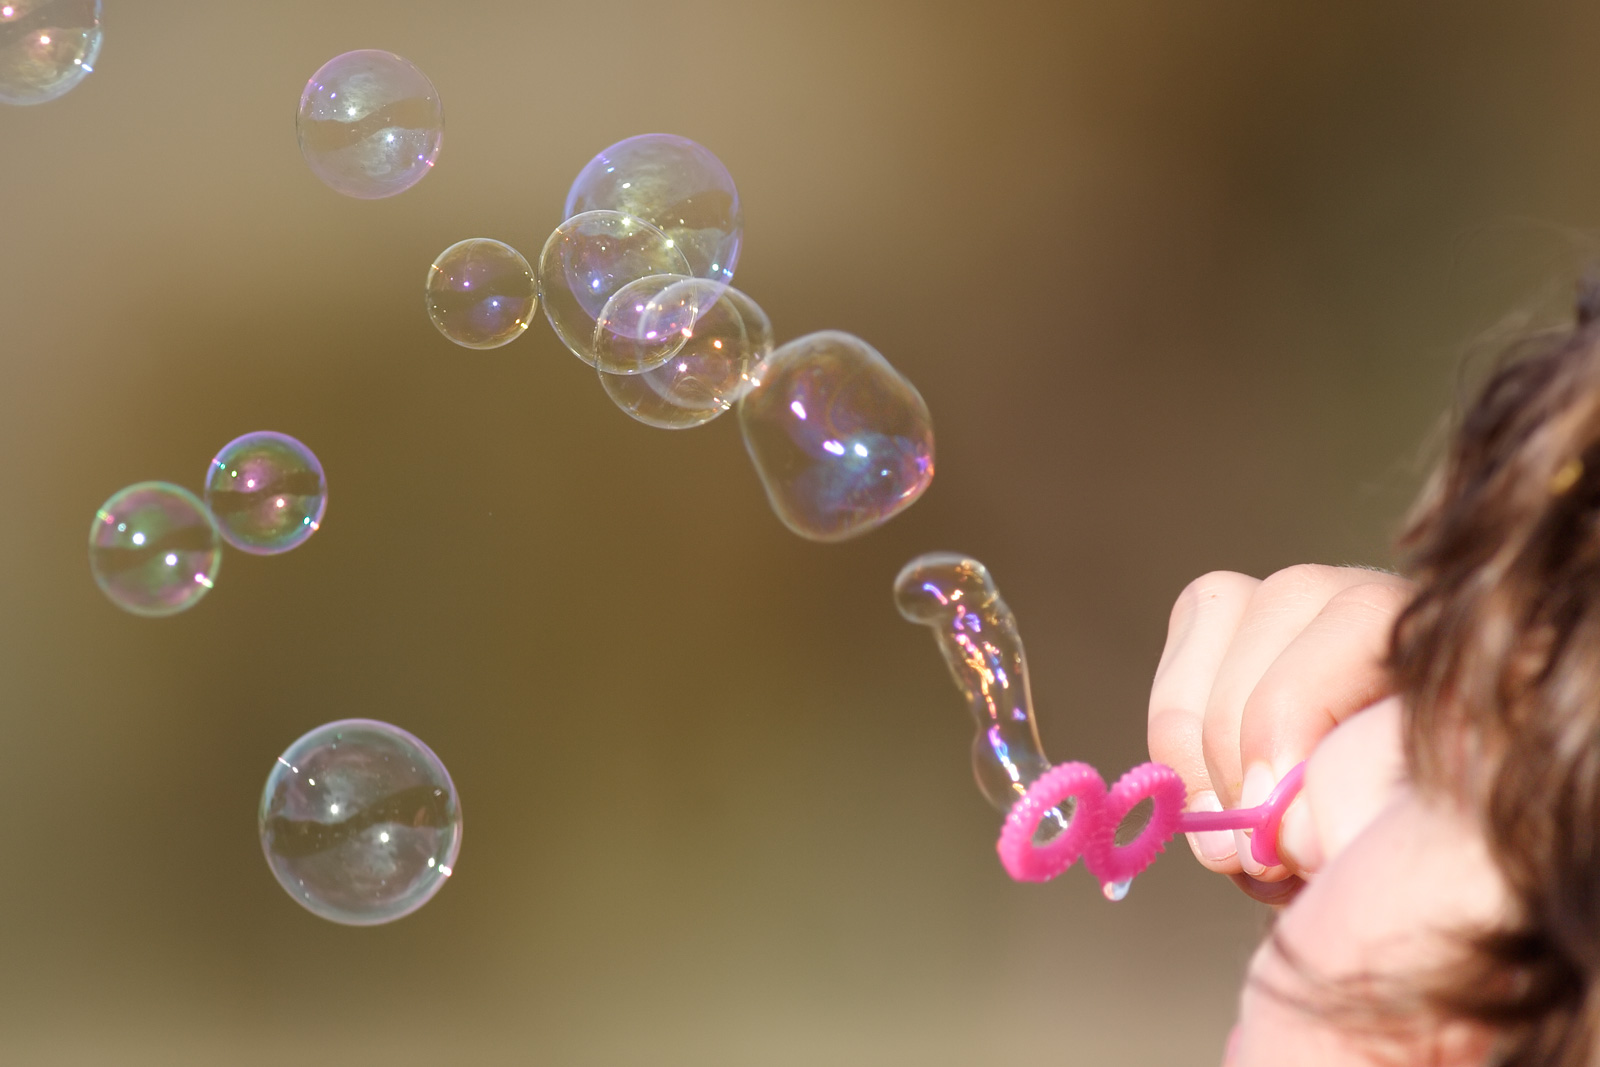
\includegraphics[width=3cm]{Girl_blowing_bubbles.jpg}
\par\noindent{\tiny{Creative Commons license, Attribution NonCommercial Unported 3.0, Fir0002/Flagstaffotos}}
\end{center}
\end{example}


\begin{lemma}\label{lemma:bubble}
Suppose that two projective plane curves \(B\) and \(C\) of order \(n\) intersect at exactly \(n^2\) points (the maximum possible by B\'ezout's theorem).
Write \(n\) as \(n=p+q\).
If exactly \(pn\) of these points lie on a curve \(E\) of degree \(p\) (again the maximum possible) then the remaining points, \(qn\) of them, lie on a curve \(F\) of degree \(q\) (again the maximum possible).
\end{lemma}
\begin{proof}
Write \(B\) and \(C\) as \(C_0\) and \(C_{\infty}\) in a pencil \(C_r\).
Pick a point \(s\) different from the intersection points of \(C_0\) and \(C_{\infty}\).
We can pick such a point, because we can replace our field by its algebraic closure if needed, or more simply by any infinite field containing.
The numbers of intersection points can't increase when we work in a larger field, since B\'ezout's theorem tells us that they are maximal already.
The point \(s\) then belongs to a unique element of the pencil, say to \(C_{r_0}\).

In particular, we can pick \(s\) to belong to \(E\).
But then \(s\) sits in \(C_{r_0}\) along with the points of \(B \cap C\) and \(s\) also sits in \(E\) along with \(pn\) points of \(B \cap C\).
So \(E\) and \(C_{r_0}\) contain \(1+pn\) points of \(B \cap C\).
By B\'ezout's theorem, the degrees of \(E\) and \(C_{r_0}\) are \(p\) and \(n\), they contain a common irreducible component.
Since \(E\) is irreducible by assumption, \(E\) is that component of \(C_{r_0}\).
So \(C_{r_0} = E \cup F\), for some curve \(F\) of degree at most \(q\), i.e. the pencil bubbles into two components.
The remaining intersection points of \(B \cap C\) don't lie in \(E\), but all lie in \(C_{r_0}\), so they lie in \(F\).
\end{proof}




\section{Polygons}\label{section:polygons}

In a projective plane, we have a concept of line, but not of line segment, or of angle or distance.
In a projective plane a \emph{triangle}\define{triangle} is a triple of points not all on the same line, together with the lines that connect them.
So a triangle looks like
\[
\begin{tikzpicture}
\clip (-1/3,-2/3) rectangle (4/3,2/3);
\draw[very thick,curveZero] (-1/3,-1/6) -- (4/3,2/3);
\draw[very thick,curveZero] (-1/3,7/3) -- (4/3,-1);
\draw[very thick,curveZero] (-1/3,1/9) -- (4/3,-4/9);
\end{tikzpicture}
\]
rather than
\[
\begin{tikzpicture}
\draw[very thick,curveZero] (0,0) -- (2/3,1/3) -- (1,-1/3) -- cycle;
\end{tikzpicture}
\]
Similarly, a \emph{quadrilateral}\define{quadrilateral} is a quadruple of points, called the \emph{vertices}, no three on the same line, with a chosen ordering defined up to cyclically permuting, so there is no first point or second point, but if you pick a point from the quadruple, there is a next point, and a next, and so on until you come back to the point you started with.
In the same way, we define a \emph{polygon}\define{polygon}.
The lines through subsequent vertices are the \emph{edges}.
We can't define the notion of a square or rectangle since there is no notion of length or angle available.


\section{Pascal's mystic hexagon}


\begingroup

\newcommand*{\drawEllipse}
{
\draw[very thick,curveZero] (0,0) ellipse (1cm and .5cm);
}

\newcommand*{\drawHexagon}
{
\foreach \i in {0,...,5}
	{
	\newcommand*{\dd}{8}
		\coordinate (p\i) at ({cos(20*\i+\dd*\i*\i)},{.5*sin(20*\i+\dd*\i*\i)}) {};
		\DrawNode{p\i}
	}
}

\newcommand*{\findFirstIntersection}
{
\coordinate (c1) at (intersection of p0--p1 and p3--p4) {};
}
\newcommand*{\findSecondIntersection}
{
\coordinate (c2) at (intersection of p1--p2 and p4--p5) {};
}
\newcommand*{\findThirdIntersection}
{
\coordinate (c3) at (intersection of p2--p3 and p5--p0) {};
}

\newcommand*{\findAllIntersections}
{
\findFirstIntersection
\findSecondIntersection
\findThirdIntersection
}


% highest x value of any coordinate of any point in the picture:
\newcommand*{\maxX}{3.5}
% lowest x value of any coordinate of any point in the picture:
\newcommand*{\minX}{-1}


\newcommand*{\showTheLine}
{
\begin{scope}[on background layer]
\draw[curveThree,very thick] (c1) -- (c3);
\draw[curveThree,very thick] (c3) -- (c2);
\end{scope}
}


\newcommand*{\firstPicture}
{
\drawEllipse
\drawHexagon
\begin{scope}[on background layer]
\draw[curveOne,very thick] (p1) -- (p2);
\draw[curveOne,very thick] (p2) -- (p3);
\draw[curveOne,very thick] (p3) -- (p4);
\draw[curveOne,very thick] (p4) -- (p5);
\draw[curveOne,very thick] (p5) -- (p0);
\draw[curveOne,very thick] (p0) -- (p1);
\end{scope}
}

\newcommand*{\secondPicture}
{
\firstPicture
\findFirstIntersection
\begin{scope}[on background layer]
\draw[curveTwo,very thick,opacity=.5] (p1) -- (c1);
\draw[curveTwo,very thick,opacity=.5] (p3) -- (c1);
\end{scope}
\DrawNode{c1}
}

\newcommand*{\thirdPicture}
{
\firstPicture
\findSecondIntersection
\begin{scope}[on background layer]
\draw[curveTwo,very thick,opacity=.5] (p1) -- (c2);
\draw[curveTwo,very thick,opacity=.5] (p5) -- (c2);
\end{scope}
\DrawNode{c2}
}

\newcommand*{\fourthPicture}
{
\firstPicture
\findThirdIntersection
\begin{scope}[on background layer]
\draw[curveTwo,very thick,opacity=.5] (p2) -- (c3);
\draw[curveTwo,very thick,opacity=.5] (p0) -- (c3);
\end{scope}
\DrawNode{c3}
}

\newcommand*{\fifthPicture}
{
\firstPicture
\findAllIntersections
\begin{scope}[on background layer]
\draw[curveTwo,very thick,opacity=.5] (p1) -- (c1);
\draw[curveTwo,very thick,opacity=.5] (p3) -- (c1);
\draw[curveTwo,very thick,opacity=.5] (p1) -- (c2);
\draw[curveTwo,very thick,opacity=.5] (p5) -- (c2);
\draw[curveTwo,very thick,opacity=.5] (p2) -- (c3);
\draw[curveTwo,very thick,opacity=.5] (p0) -- (c3);
\end{scope}
\DrawNode{c1}
\DrawNode{c2}
\DrawNode{c3}
}

\newcommand*{\sixthPicture}
{
\fifthPicture
\showTheLine
}



\newcommand{\Pascal}[1]{%
\par\noindent%
\begin{center}
\begin{tikzpicture}
% Draw a strut to make all of the diagrams have the same width, so the same x coordinate in each diagram gives a point the same distant across the page.
%\begin{scope}[on background layer]
\draw[white,opacity=0] (\minX,0) -- (\maxX,0); 
%\fill[gray!20,draw=black] (\minX,-3) rectangle (\maxX,4.5);
%\end{scope}
\IfStrEqCase{#1}{%
{1}%
{%%
\firstPicture
}%%
{2}%
{%
\secondPicture
}%
{3}%
{%%
\thirdPicture
}%%
{4}%
{%%
\fourthPicture
}%%
{5}%
{%%
\fifthPicture
}%%
{6}%
{%%
\sixthPicture
}%%
{7}%
{%%
\seventhPicture
}%%
{8}%
{%%
\eighthPicture
}%%
}%% end IfStrEqCase
\end{tikzpicture}
\end{center}
}

Draw a hexagon with vertices sitting inside a conic. \Pascal{1}
Since there is an even number of sides, each side has an ``opposite'' side, half way around the hexagon.
Pick a side and its opposite, and draw lines joining them. \Pascal{2}
The same for the next pair of opposite sides. \Pascal{3}
And finally for the third pair of opposite sides. \Pascal{4}
Draw all of these lines together in one picture. \Pascal{5}
Mysteriously, all three intersection points lie on a line. \Pascal{6}

\endgroup

\begin{theorem}
Given a hexagon in the projective plane over a field, the intersection points of opposite sides lie on a line.
\end{theorem}
\begin{proof}
Let \(B\) be the reducible cubic curve consisting of three of the lines, no two of them in succession (for example, the first, third and fifth lines).
Let \(C\) be the reducible cubic curve consisting of the remaining three lines of the hexagon.
Let \(E\) be the quadric.
The result follows immediately from lemma~\vref{lemma:bubble}.
\end{proof}


\section{The space of curves of given degree}

Consider the vector space \(V_d\) of homogeneous polynomials of degree \(d\) in \(3\) variables.
Each such polynomial has a coefficient of \(x^a y^b z^c\) as long as \(a+b+c=d\).
Imagine that we take \(d+2\) sticks sitting in a row.
Colour 2 of them white and the rest black.
Take \(a\) to be the number of black sticks before the first white one, \(b\) the number of black sticks between the two white ones, and \(c\) the number of black sticks after the second white one.
Clearly \(a+b+c=d\).
So the dimension of \(V_d\) as a vector space is 
\[
\binom{d+2}{2}.
\]
But since the equation \(p_C=0\) of a curve \(C\) is defined only up to rescaling, the curves of degree \(d\) are identified with points of \(\Proj[d^*]{k}\) where 
\[
d^* = -1+\binom{d+2}{2}=\frac{d(d+3)}{2}.
\]

\[
\begin{array}{@{}rr@{}}
\toprule 
d & d^* \\
\midrule
1  &  2  \\
 2  &  5  \\
 3  &  9  \\
 4  &  14  \\
 5  &  20  \\
 6  &  27  \\
 7  &  35  \\
 8  &  44  \\
 9  &  54  \\
\bottomrule 
\end{array}
\]
For example, the set of lines in \(\Proj[2]{k}\) is a 2-dimensional projective space, a projective plane, the \emph{dual projective plane}\define{dual!projective plane}\define{projective!plane!dual}.
More generally, our projective space \(\Proj[d^*]{k}\) contains all curves of degree \(d\), reducible or irreducible.

A pencil\SubIndex{pencil} \(C_r = (p=rq)\) of two curves \(B\) and \(C\) is just a line inside \(\Proj[d^*]{k}\).
More generally, a \emph{linear system}\define{linear!system} is collection of plane curves whose equations form a projective linear subspace in \(\Proj[d^*]{k}\).


The condition that a point \(q_0=(x_0,y_0,z_0)\) lies in a curve \(C=\pr{c(x,y,z)=0}\) is a linear equation \(c(x_0,y_0,z_0)=0\) on the coefficients of the polynomial \(c(x,y,z)\), so is satisfied by a linear projective hyperplane inside \(\Proj[d^*]{k}\).
For example, the condition that a point lie in a line is one equation, so determines a line in the dual projective plane.
Similarly, the condition that a curve has order at least \(k\) at a point \(q_0\) of the plane is a collection of \(k(k+1)/2\) linearly independent equations, killing the terms in the Taylor series up to order \(k\) (if we arrange that \(q_0\) is the origin, for example).
A collection of points \(p_1, p_2, \dots, p_n\) in the projective plane is in \emph{general position}\define{general position} for curves of degree \(d\) if the linear system of curves passing through them has either (1) the minimal dimension possible \(d(d+3)/2-n\) if this quantity is not negative and (2) is empty otherwise.

\begin{lemma}\label{lemma:general.position.defined}
The definition of general position makes sense, in that if we fix \(n\) points, then the linear system consisting of all degree \(d\) curves through those points has dimension at least 
\[
d^*-n=\frac{d(d+3)}{2}-n.
\]
After perhaps replacing our field with an infinite extension field, if \(d^*-n \ge 0 \) then equality is acheived for some collection of \(n\) points, while if \(d^*-n<0\) then there is a collection of \(n\) points not lying on any curve of degree \(d\).
In particular, if \(d^*=n\), then (after perhaps an infinite field extension) there is a set of \(n\) points for which there is a unique curve of degree \(d\) passing through those \(n\) points.
\end{lemma}
\begin{proof}
The proof is by induction.
For \(d=1\), there is a pencil of lines through a point (\(n=1\)) and a unique line through any 2 points (\(n=2\)) and no line through 3 or more points, if we pick our 3 points correctly.
Suppose that the result is true for all values of \(n\) and \(d\) less than some particular choices of \(n\) and \(d \ge 2\).
Note that 
\[
d^*=\frac{d(d+3)}{2} = d+1+\frac{(d-1)(d-1+3)}{2} = d+1+(d-1)^*.
\]
Pick \(d+1\) points on a line \(L\), and then pick \((d-1)^*\) points in general position, so that they lie on a unique curve \(C\) of degree \(d-1\).
By B\'ezout's theorem, the line \(L\) is a component of any curve \(D\) of degree \(d\) through the first \(d+1\) points.
Therefore such a curve \(D\) is just \(C \cup L\).
Hence \(D\) is the unique curve of its degree through the given points.
So through some collection of \(d(d+3)/2\) points, there is a unique curve of degree \(d\).
If we add any more points, choosing them not to lie on the that curve, then there is no curve of degree \(d\) through those points.
If we take away any points, say down to some number \(n\) of point, then the dimension goes up by at most one for each removed point, giving us our result by induction.
\end{proof}
 
\begin{example}
Through any 2 points there is precisely one line: 
\begin{tikzpicture} 
\draw[axisColor,very thick] (0,0) -- (1,0); 
\DrawDot{0}{0} 
\DrawDot{1}{0} 
\end{tikzpicture}
\end{example}
\begin{example}
Through any 5 points in general position, there is precisely one conic.
\inputinexample{5-points-on-conic}
\end{example}
\begin{example}
Through any 9 points in general position, there is precisely one cubic.
\inputinexample{cubic-curve-5}
\end{example}
\begin{example}
Through any 14 points in general position, there is precisely one quartic.
\end{example}
\begin{example}
Through any 20 points in general position, there is precisely one quintic.
\end{example}

\begin{lemma}\label{lemma:conics.5.points}
Through any 5 points in the plane, there is a conic.
\begin{itemize}
\item
No three of the points lie on a line just when the conic is irreducible.
\item
No four of the points lie on a line just when the conic is unique.
\item
Four but not five of the points lie on a line just when the conics through all five form a pencil, with each curve in the pencil being a pair of lines: the line through the four colinear points, and any line through the fifth point.
\item
All five points lie on a line just when the conics form a 2 dimensional linear system, with each curve in the system being a pair of lines: the line through the five points, and any other line.
\end{itemize}
\end{lemma}
\begin{proof}
The space of conics through 4 points has dimension at least \(d^*-4=2^*-4=5-4=1\).
Indeed there is a pair of lines covering those 4 points.
Add a fifth point, not colinear with any three of the other four.
The condition of containing the fifth point is an additional linear equation on the quadratic polynomial of the conic, independent of those for the first four points, as it is not satisfied for that pair of lines.
So the linear system of conics through the five points is a smaller dimensional projective space, but still not empty.

If no three of the points are colinear, then repeating the argument above, each point adds an independent condition, not a linear combination of the others, so there is a unique conic through the five points.
If that conic is reducible, it is a pair of lines, and then all five points lie on two lines, so at least three points lie on one of the lines.
Since some line contains three of the points, by B\'ezout's theorem, that line is a component of the conic, so the conic must be a pair of lines, one of which is determined.

If no line contains four of the points, then each line is determined by the two points it contains which are not on the other line, and the conic is uniquely determined.
\end{proof}


A points \(p_1,p_2,\dots,p_n\) in the plane \emph{impose independent conditions on curves of degree \(d\)}\define{independent conditions} if the linear system of curves through those points has dimension \(d^*-n\) (or is empty if \(d^*-n<0\)).
Lemma~\vref{lemma:general.position.defined} says that (after perhaps a field extension) failure to impose independent conditions on curves of degree \(d\) occurs just when the linear system of curves through those points has dimension more than \(d^*-n\) (or is not empty, if \(d^*-n<0\)), and also says that we can choose \(n\) points that impose independent conditions.
We want to examine the failure of small numbers of points to impose independent conditions.

Imagine we try to prove that points \(p_1,p_2,\dots,p_n\) impose independent conditions on curves of degree \(d\).
Suppose we prove that there is a curve of degree \(d\) passing through \(p_1,p_2,\dots,p_{n-1}\) but not \(p_n\).
In the vector space of degree \(d\) polynomials, the condition of passing through \(p_n\) as well is an additional linear equation not always satisfied, so cuts out a linear subspace of one lower dimension.
If the choice of which point is \(p_n\) is arbitrary, then the same will hold for any of the points \(p_i\) in place of \(p_n\), giving \(n\) linearly independent equations, i.e. a linear subspace of \(n\) lower dimensions, so the points impose independent conditions on curves of degree \(d\).

\begin{theorem}\label{theorem:independence}
Suppose that \(p_1,p_2,\dots,p_n\) are distinct points in the plane, and \(n \le 2d+2\).
Then these points fail to impose independent conditions on curves of degree \(d\) just when either 
\begin{itemize}
\item
\(d+2\) of the points are colinear or
\item
\(n=2d+2\) and the points \(p_1,p_2,\dots,p_n\) lie on a conic.
\end{itemize}
\end{theorem}
\begin{proof}
Suppose that \(d+2\) of the points are colinear, say on a line \(L\), and say they are \(p_1,p_2,\dots,p_{d+2}\).
By B\'ezout's theorem, any curve of degree \(d\) containing those points contains \(L\) so has equation factoring into a product of the equation of \(L\) and an equation of degree \(d-1\).
The set of curves of degree \(d\) containing \(L\) is a projective space of dimension \((d-1)^*\), and so imposing that our curve has degree \(d\) and contains \(L\) is imposing \(d^*-(d-1)^*=d+1\) conditions.
The remaining points are \(p_{d+3},\dots,p_n\), so \(n-(d+2)\) points, and so together impose at most \(n-(d+2)\) conditions, i.e. \(p_1,\dots,p_n\) together impose at most \(d+1+n-(d+2)=n-1\) conditions at most, so the points fail to impose independent conditions.

Suppose that \(n=2d+2\) and that the points \(p_1,p_2,\dots,p_n\) lie on a conic.
Construct a curve of degree \(d\) through the points by constructing a conic through the points, and then constructing any curve of degree \(d-2\), i.e. \((d-2)^*\) dimensions of curves at least.
If the points were to impose independent conditions, we would have \(d^*-n=d^*-(2d+2)\) dimensions of curves.
But
\[
(d-2)^* = \frac{d^2-d-2}{2} > \frac{d^2-d-4}{2} = d^*-n.
\]

Now we suppose that \(p_1,p_2,\dots,p_n\) fail to impose independent conditions, and that \(n \le 2d+2\).
Some special cases to get started:
\begin{itemize}
\item \(n=0\): no conditions, so failure is impossible, i.e. \(d^*\) dimensions of curves.
\item \(n=1\): one point cannot fail to impose independent conditions, as there is a curve of any degree \(d > 0\) not passing through that point (at least after a field extension).
\item \(n=2\): for any two points, take \(d\) lines through one point none of which contain the other (at least after a field extension). Their union is a degree \(d\) curve.
\item \(n=3\): if the points are not colinear, a line through two of the points and not the third, taken \(d\) times, is a degree \(d\) curve.
If the points are colinear, and \(d=1\), they fail to impose independent conditions, but satisfy our theorem.
So we can suppose that the points are colinear, and \(d \ge 2\).
Pick three more points \(q_1,q_2,q_3\) so that the five points \(p_1,p_2,q_1,q_2,q_3\) contain no three colinear points.
(We can do this after perhaps a field extension.)
The conic through these five points is irreducible, so does not contain the line through \(p_1,p_2,p_3\), by B\'ezout's theorem.
Add some lines to that conic, none of them through \(p_3\), to get a degree \(d\) curve through \(p_1,p_2\) missing \(p_3\).
\item \(d=1\): degree \(d\) curves are lines. 
We have \(n\le 2d+2=4\) points.
Our \(n\) points fail to impose independent conditions on lines just when either 
\begin{itemize}
\item
\(n\ge 3\) and the points are colinear or
\item
\(n=4\): all 4 points lie on a conic, for example on a pair of lines.
\end{itemize}
\item \(d=2\): degree \(d\) curves are conics.
Suppose that no \(d+2=4\) points lie on a line.
By hypothesis, \(n \le 2d+2=6\), so we need to consider \(n=4,5,6\).
The conic through any 5 of the points is unique, by lemma~\vref{lemma:conics.5.points}.
\begin{itemize}
\item
\(n=5\): the points impose independent conditions because \(d^*-n=0\) and the space of conics through all 5 points is zero dimensional.
\item
\(n=4\): add a fifth point not on any line through the four points, and get a unique conic through all five, so the five points impose independent conditions, and so the four points do.
\item
\(n=6\): any five of the points lie on a conic, so the sixth point fails to give an independent condition just when all six lie on the same conic.
\end{itemize}
\item \(n \le d+1\): pick lines \(L_1,L_2,\dots,L_{n-1}\), each line \(L_i\) passing through the point \(p_i\) and no other of the points.
Then \(C\defeq L_1 \cup L_2 \cup \dots \cup L_{n-1}\) has degree \(n-1\).
If \(n-1<d\) then pick some curve \(D\) of degree \(d-n+1\), not passing through \(p_n\), and we get a curve \(C \cup D\) of degree \(d\) through all but one point.
To get this to work, we need \(n-1\le d\), i.e. \(n\le d+1\).
\end{itemize}

By induction, suppose we have proven our result for all smaller values of \(d\), and, for the given \(d\), for all smaller values of \(n\).
Suppose that among \(p_1,\dots,p_n\), the points \(p_1,\dots,p_{d+1}\) lie on a line \(L\).
If any more of our points lie on that line, the result is proven.
Let \(d'\defeq d-1\) and \(n'\defeq n-(d+1)\) and let
\[
p_1',\dots,p_{n'}'
\]
be the points
\[
p_{d+2},\dots,p_n.
\]
If \(p'_1,\dots,p'_{n'}\) impose independent conditions on curves of degree \(d'\), then we find a curve \(C\) of degree \(d'=d-1\) through all but one of \(p_{d+2},\dots,p_n\), and then \(L \cup C\) has degree \(d\) and passes through all but one of \(p_1,\dots,p_n\), so \(p_1,\dots,p_n\) are independent conditions.
Hence \(p'_1,\dots,p'_{n'}\) fail to impose independent conditions.

By induction, either 
\begin{itemize}
\item
\(d'+2\) of the points \(p'_1,\dots,p'_{n'}\) are colinear or 
\item
\(n'=2d'+2\) and the points \(p'_1,\dots,p'_{n'}\) lie in a conic.
\end{itemize}
The second possibility, \(n'=2d'+2\), expands out to become \(n=3d+1\).
But \(n \le 2d+2\), which forces \(d\le 1\), not possible.
Hence \(d'+2\) of the points \(p'_1,\dots,p'_{n'}\) are colinear, i.e. \(d+1\) of the points \(p_{d+2},\dots,p_n\) are colinear, say on a line \(L'\).
So the conic \(L \cup L'\) contains \(2d+2\) of the points \(p_1,\dots,p_n\).
But \(n \le 2d+2\), so \(n=2d+2\).
So we have a contradiction: no \(d+1\) of our points are colinear.

Suppose that some number \(\ell\) of our points are colinear, say \(p_1,p_2,\dots,p_{\ell}\).
Let \(d'\defeq d-1\) and \(n'\defeq n-\ell\) and let
\[
p_1',\dots,p_{n'}'
\]
be the points
\[
p_{\ell+1},\dots,p_n.
\]
If \(p'_1,\dots,p'_{n'}\) impose independent conditions on curves of degree \(d'\), then we find a curve \(C\) of degree \(d'\) through all but one of \(p'_1,\dots,p'_{n'}\).
Then \(L \cup C\) has degree \(d\) and passes through all but one of \(p_1,\dots,p_n\), so \(p_1,\dots,p_n\) are independent conditions, a contradiction.
Hence \(p'_1,\dots,p'_{n'}\) fail to impose independent conditions.

By induction, either 
\begin{itemize}
\item
\(d'+2\) of the points \(p'_1,\dots,p'_{n'}\) are colinear or 
\item
\(n'=2d'+2\) and the points \(p'_1,\dots,p'_{n'}\) lie in a conic.
\end{itemize}
The first possibility, \(d+1\) of the points are colinear, we have already ruled out.
So \(n'=2d'+2\), expands out to become \(n=2d+2+\ell-2\).
But \(n \le 2d+2\), which forces \(\ell\le 2\).
So no \(3\) of our points are colinear.

Suppose that \(p_3,\dots,p_n\) impose independent conditions on curves of degree \(d-1\).
Then there is a curve \(C\) of degree \(d-1\) through all of \(p_4,\dots,p_n\) and not through \(p_3\).
But then \(p_1p_2 \cup C\) has degree \(d\) and misses \(p_3\), a contradiction.
So any \(n-2\) of our points fail to impose independent conditions on curves of degree \(d-1\).
We let \(n'=n-2\) and \(d'=d-1\), and apply induction to see that \(n'\le 2d'+2\), so either
\begin{itemize}
\item \(d'+2\) points are colinear, or 
\item
\(n'=2d'+2\) and \(p_3,\dots,p_n\) lie on a conic.
\end{itemize}
The first case expands out to \(d+1\) points are colinear, a contradiction to the results above.
The second case expands out to \(n=2d+2\) and \(p_3,\dots,p_n\) lie on a conic.
But this is true for any reordering of our points: any set of \(n-2\) of our points lie on a conic.
If \(d=1\) or \(d=2\), we have already checked our result above.
For \(d \ge 3\), since we have found that \(n=2d+3 \ge 9\), so \(n-2 \ge 7\).
If you choose \(n-2\) points and I choose \(n-2\) points, they must have at least \(n-4\ge 5\) points in common.
Any 5 of our points lie on at most one conic, since no three are colinear, by lemma~\vref{lemma:conics.5.points}.
So all \(n\) points lie on a conic.
\end{proof}





\chapter{Elliptic curves}

\epigraph[author={Serge Lang}, source={Elliptic Curves: Diophantine Analysis}]{It is possible to write endlessly on elliptic curves. (This is not a threat.)}\SubIndex{Lang, Serge}


\section{Cubic curves}

\begin{theorem}[Chasles]\label{theorem:Chasles}\define{theorem!Chasles}\define{Chasles theorem}
Suppose that \(C_1\) and \(C_2\) are plane cubic curves intersecting at 9 points over the algebraic closure of the field.
Every plane cubic curve passing through any 8 of those points passes through all 9.
The plane cubic curves passing through those 9 points are precisely the pencil through \(C_1\) and \(C_2\).
\end{theorem}
\begin{proof}
By theorem~\vref{theorem:independence}, with \(n=8\) and \(d=3\), either 
\begin{enumerate}
\item
8 of the points impose independent conditions or
\item
5 of the points are colinear or
\item
all 8 of the points lie on a conic.
\end{enumerate}
If 7 of the points lie on a conic, then by B\'ezout's theorem that conic lies in both \(C_1\) and \(C_2\), so \(C_1\) and \(C_2\) have infinitely many points in common, a contradiction.
If 4 of the points lie on a line, then by B\'ezout's theorem that line lies in both \(C_1\) and \(C_2\), so \(C_1\) and \(C_2\) have infinitely many points in common, a contradiction.
So all 8 points inmpose independent conditions, i.e. the projective space of cubics through all \(8\) points has dimension \(3^*-8=1\).
Since \(C_1 \ne C_2\), the projective space of cubics through all \(9\) points has dimension at least 1: the pencil through \(C_1\) and \(C_2\) is 1-dimensional.
But the family through all 9 points is a projective subspace of the family through all 8 points.
Both projective spaces have the same dimension, hence these two projective spaces are equal.
\end{proof}


\begin{center}
\documentclass{standalone}
\usepackage{tikz}
\usepackage{pgfplots}
\pgfplotsset{compat=1.12,width=7cm}%
\begin{document}
\begin{tikzpicture}
\begin{axis}[hide axis,xmin=-2,xmax=2,ymin=-2,ymax=2]
\newcommand{\RRR}{1.8}
\newcommand{\lineclr}{gray!30}
\draw[\lineclr] 
	(\RRR,0) 
-- ({-\RRR},0);
\newcommand{\curveclr}{gray}
  \addplot[domain=-1:0,\curveclr,samples=200]{sqrt((x+1)*x*(x-1))};%
  \addplot[domain=-1:0,\curveclr,samples=200]{-sqrt((x+1)*x*(x-1)))};%
  \addplot[domain=1:2,\curveclr,samples=200]{sqrt((x+1)*x*(x-1)))};%
  \addplot[domain=1:2,\curveclr,samples=200]{-sqrt((x+1)*x*(x-1)))};%
  \fill[gray!20,draw=gray] (axis cs:0,0) circle (1.3pt);
  \fill[gray!20,draw=gray] (axis cs:1,0) circle (1.3pt);
  \fill[gray!20,draw=gray] (axis cs:-1,0) circle (1.3pt);
\end{axis}
\end{tikzpicture}
\end{document}

\end{center}
For any two distinct points \(p, q\) of a cubic curve \(C\), the line through \(p\) and \(q\) intersects \(C\) in three points; let \(r\) be the third point.
If \(p\) and \(q\) are defined in some field \(k\), then so is the line through \(p\) and \(q\).
Suppose that \(C\) is also defined over \(k\).
On that line, parameterized over \(k\) as \(y=mx+b\), the cubic equation of \(C\) (having coefficients over \(k\)) restricts to have at least two roots in \(k\), corresponding to the points \(p\) and \(q\).
So that cubic polynomial on the line factors into linear factors over \(k\).
That third root gives the location of \(r\) on that line: the point \(r\) is also defined over \(k\).

We can extend this definition to allow \(p=q\), by taking \(r\) to be the point of \(C\) at which the tangent line to \(\ell\) to \(C\) at \(p\) touches \(C\) again. 
\begin{center}
\documentclass{standalone}
\usepackage{tikz}
\usepackage{pgfplots}
\pgfplotsset{compat=1.12,width=7cm}%
\usepackage{xparse}
\colorlet{curveZero}{gray!75}
\colorlet{curveOne}{blue!60}
\colorlet{curveTwo}{brown!50!gray}
\colorlet{curveThree}{green!40!gray}
\colorlet{curveFour}{red!50!gray}
\NewDocumentCommand\DrawDotInPlot{O{}mmO{}}%
{%
\fill[gray!20,draw=gray] (axis cs:{#2},{#3}) circle (1.3pt) node[above,black,#4] {\(#1\)};%
}%
\NewDocumentCommand\DrawDot{O{}mmO{}}%
{%
\fill[gray!20,draw=gray] ({#2},{#3}) circle (1.3pt) node[above,black,#4] {\(#1\)};%
}%
\NewDocumentCommand\DrawNode{O{}m}%
{%
\fill[gray!20,draw=gray] (#2) circle (1.3pt) node[above,black] {\(#1\)};%
}%
\colorlet{axisColor}{gray!50}
\tikzstyle{shapeZero}=[fill=curveZero,opacity=.4]
\tikzstyle{shapeOne}=[fill=curveOne,opacity=.4]
\tikzstyle{shapeTwo}=[fill=curveTwo,opacity=.4]
\tikzstyle{shapeThree}=[fill=curveThree,opacity=.4]
\tikzstyle{groupElementLabel}=[minimum size=2.4em]
\tikzstyle{groupElement}=[minimum size=2.4em,shapeZero,draw=curveZero]
\tikzstyle{cosetOne}=[minimum size=2.4em,shapeOne,draw=curveOne]
\tikzstyle{cosetTwo}=[minimum size=2.4em,shapeTwo,draw=curveTwo]


\begin{document}
\begin{tikzpicture}
\begin{axis}[hide axis,xmin=-2,xmax=2,ymin=-2,ymax=2]
\newcommand{\fn}[1]{sqrt((#1+1)*(#1)*(#1-1))}
\newcommand{\xnought}{-.35}
\pgfmathsetmacro{\ynought}{0.554188596057335}
\pgfmathsetmacro{\slope}{-0.570654109900308}
\newcommand{\xone}{-1.8}
\pgfmathsetmacro{\yone}{1.38163705541278}
\newcommand{\xtwo}{1.8}
\pgfmathsetmacro{\ytwo}{-0.672717740228328}
\draw[axisColor] 	(axis cs:{\xone},{\yone}) -- (axis cs:{\xtwo},{\ytwo});
  \addplot[very thick,domain=-1:0,curveZero,samples=200]{sqrt((x+1)*x*(x-1))};%
  \addplot[very thick,domain=-1:0,curveZero,samples=200]{-sqrt((x+1)*x*(x-1)))};%
  \addplot[very thick,domain=1:2,curveZero,samples=200]{sqrt((x+1)*x*(x-1)))};%
  \addplot[very thick,domain=1:2,curveZero,samples=200]{-sqrt((x+1)*x*(x-1)))};%
  \DrawDotInPlot[p]{\xnought}{\ynought}
  \DrawDotInPlot[r]{1.02564611314611}{-0.230829512177879}[below left]
\end{axis}
\end{tikzpicture}
\end{document}

\end{center}

With a little algebra by hand, and some sage code to solve the mess, we can find the intersection points of tangent lines.
Consider the curve
\[
C=(y^2-(x+1)x(x-1))
\] 
and the point \(p\) with \(p=(x,y)\) with \(x=-35/100\):
\begin{sageblock}
X=-35/100
Y=sqrt((X+1)*X*(X-1))
# The slope of the tangent line is given by implicit differentation.
M=(3*X^2-1)/(2*Y)
# Write the equation of the curve restricted to the tangent line.
x=var('x')
f=(Y+M*(x-X))^2-(x+1)*x*(x-1)
print("The tangent line strikes the curve at ",solve(f,x))
XX=(201601/196560)
YY=-sqrt((XX+1)*XX*(XX-1))
print("The other intersection point is ",XX.n(),YY.n())
plot(f,x,-2,2)
\end{sageblock}




\section{Elliptic curves}

A \emph{elliptic curve}\define{elliptic curve}\define{curve!elliptic} over a field \(k\) is a smooth plane cubic curve \(C\) defined over \(k\) with a chosen point \(o\) of \(C\), also defined over \(k\), which we think of as the ``origin'' of \(C\).
Given any point \(p\) of \(C\), the line \(op\) contains three points of \(C\) (counting with multiplicity if needed), say \(p,o,\bar{p}\).
Define the \emph{addition} of points \(p,q\) by taking the line \(pq\), which then intersects \(C\) at 3 points, say \(p,q,r\), and then defining \(p+q\) to be \(\bar{r}\), so \(p+q,r,o\) are the three points at which a line intersects \(C\).
Danger: note that this addition is \emph{not} the same as adding the coordinates of the points, as you would do in linear algebra.

What if \(p=q\)?
The tangent line to \(C\) at \(p\) intersects \(C\) at some point not equal to \(p\), say \(r\), and define \(p+p=\bar{r}\).

\begin{theorem}
Any elliptic curve is an abelian group under the addition operation.
\end{theorem}
\begin{proof}
If \(p,q,r\) are the points at which a line intersects a cubic \(C\), then so are \(q,p,r\), and so \(p+q=\bar{r}=q+p\).
By definition, \(p,o,\bar{p}\) are on a line, so \(\bar{\bar{p}}=p\) and so \(p+o=\bar{\bar{p}}=p\).

Consider the point \(\bar{o}\), i.e. so that the line \(\bar{o}o\) is the tangent line to \(C\) at \(o\).
Let \(-p=\overline{p+\bar{o}}\), i.e. \(-p,p,\bar{o}\) are on a line.
So then \(p+(-p)=\bar{\bar{o}}=o\).

Any equation like \(r+q=p+q\) forces the points \(r,q,\overline{r+q}\) to be \(r,q,\overline{p+q}\), and hence to be \(p,q,\overline{p+q}\), so \(p=r\), we can cancel.

By definition of addition, for any two points \(p,q\) of \(C\),
\[
p,\overline{p+q},\overline{p+\overline{p+q}}
\]
lie in a line, while 
\[
p,q,\overline{p+q}
\]
do as well, so 
\[
q=\overline{p+\overline{p+q}},
\]
i.e.
\[
\bar{q}=p+\overline{p+q},
\]
a ``funny cancellation''.

Take three points \(p,q,r\) of \(C\).
We want to prove that \(p+(q+r)=(p+q)+r\).
Suppose that \(p=o\) or \(q=o\) or \(r=o\) or \(p=r\).
The equation \(p+(q+r)=(p+q)+r\) follows from any of these.
So we can suppose that none of these is satisfied.

Define lines
\begin{align*}
L_1 &= p(q+r), \\
L_2 &= rq, \\
L_3 &= o(p+q), \\
L'_1 &= r(p+q), \\
L'_2 &= pq, \\
L'_3 &= o(r+q).
\end{align*}

Note that \(p,q+r\) lie on \(L_1\), and so therefore does \(\overline{p+(q+r)}\).
Similarly,
\begin{align*}
p,q+r,\overline{p+(q+r)} & \in L_1, \\
r,q,\overline{q+r} & \in L_2, \\
o,p+q,\overline{p+q} & \in L_3, \\
r,p+q,\overline{(p+q)+r} & \in L'_1, \\
p,q,\overline{p+q} & \in L'_2, \\
o,q+r,\overline{q+r} & \in L'_3.
\end{align*}

Suppose that \(L_1 = L_1'\).
So the points \(p,q+r,\overline{p+(q+r)}\) are some permutation of the points \(r,p+q,\overline{(p+q)+r}\).
This forces \(p=r\) or \(p=p+q\) or \(q+r=r\) or \(q+r=p+q\), and after cancellation these becomes \(p=r\) or \(q=o\), contradicting our hypotheses.

So \(L_1 \ne L_1'\).
Take the point \(s\) where \(L_1\) and \(L_1'\) intersect.
If \(s\) lies on \(C\), then \(s\) lies on \(p,q+r,s\), so \(\bar{s}=p+(q+r)\), but also \(s\) lies on \(r,p+q,s\), so \(\bar{s}=(p+q)+r\).
So \(s\) lies on \(C\) just when \(p+(q+r)=(p+q)+r\).

Consider the 8 points \(o,p,q,r,q+r,p+q,\) and a ninth point \(s\).
The cubic \(L_1 \cup L_2 \cup L_3\) contains all 9 points, as does the cubic \(L_1' \cup L_2' \cup L_3'\).
Suppose that these cubics have no component in common.
Then by Chasles's theorem (theorem~\vref{theorem:Chasles}), the plane cubics containing the 8 points contain all 9, so \(s\) belongs to \(C\).

Suppose that these cubics share a component, say \(L_i = L_j'\).
The 3 points of \(C\) on \(L_i\) and the 3 points on \(L_j'\) must be the same 3 points.
No other point of the cubic \(C\) can lie on that line, by B\'ezout's theorem.
So the remaining 5 points lie on the other lines.
Each pair of remaining lines is a conic.
By lemma~\vref{lemma:conics.5.points}, these conics are equal or share a common line through 4 of the points.
But we can't have 4 points of \(C\) on the same line, by B\'ezout's theorem.
So these conics are equal, i.e. all three lines \(L_1,L_2,L_3\) are the same as \(L_1',L_2',L_3'\) up to reordering.

We know that \(L_1 \ne L_1'\), so \(L_1=L_2'\) or \(L_1=L_3'\).
Swapping \(p\) and \(r\) swaps primed and unprimed lines.

If \(L_2=L_2'\), the points \(r,q,\overline{q+r}\) are the same as \(p,q,\overline{p+q}\), up to reordering.
If this forces \(r=p\), we have seen that \(p+(q+r)=(p+q)+r\) follows.
Otherwise, we find \(\overline{q+r}=p\) and \(r=\overline{p+q}\), and then
\[
p+(q+r)=p+\bar{p}=\bar{o},
\]
and
\[
(p+q)+r=\bar{r}+r=\bar{o}.
\]
So we can assume that \(L_2 \ne L_2'\).

If \(L_3=L_3'\), the points \(o,p+q,\overline{p+q}\) are the same as \(o,r+q,\overline{r+q}\).
Since we suppose that \(p \ne r\), \(r+q=\overline{p+q}\).
By funny cancellation,
\[
p+(q+r)=p+\overline{p+q}=\bar{q},
\]
while
\[
(p+q)+r=\overline{q+r}+r=r+\overline{r+q}=\bar{q},
\]
so again \(p+(q+r)=(p+q)+r\).

If \(L_2=L_3'\) then \(r=o\) or \(q=o\), a contradiction.

Hence \(L_1, L_2, L_3\) must be some permutation of \(L_1',L_2',L_3'\), but we can't have \(L_1=L_1'\) or \(L_2=L_2'\) or \(L_2=L_3'\) or \(L_3=L_3'\).
So \(L_1=L_3'\).
Permutation of \(p\) and \(r\) then forces \(L_3=L_1'\), so \(L_2=L_3'\), a contradiction.
\end{proof}



\begin{example}
We always take an elliptic curve to be a smooth cubic \(C\) with a chosen point \(o \in C\), giving an addition operation as above.
If we pick some other point \(o'\) of our cubic curve \(C\) to be the ``origin'' of an elliptic curve, then we get another addition operation, say \(+'\).
The map
\[
p \in C \mapsto p+(o'-o),
\]
using the operations defined above is an isomorphism of groups from \(C\) with \(+\) to \(C\) with \(+'\).
So the choice of point \(o\) is not very important.
\end{example}

\chapter{The tangent line}\label{chapter:tangent.line}

\section{Lines crossing a curve}

\begin{proposition}
Pick an irreducible plane algebraic curve \(C\) of degree \(d\) and a point \(p\) of the plane not lying on \(C\).
Among all of the lines through \(p\), every one of them strikes \(C\) in exactly \(d\) distinct points, except for at most \(d(d-1)\) lines.
\end{proposition}
\begin{proof}
First assume that \(C\) is irreducible.
Arrange that the point \(p\) lies at the origin in an affine chart, so that the lines through \(p\) are those of the form \(y=mx\) or \(x=0\).
Also arrange that \(C\) is not entirely on the line at infinity, so contains some finite points.
From the equation \(q(x,y)=0\) of the curve \(C\), the intersections lie on \(q(x,mx)=0\), a polynomial of degree at most \(d\) in \(x\).
This polynomial is not the zero polynomial, because the origin does not lie on \(C\).
Therefore the number of intersections is \(d\).
The multiplicities will all be 1 except at values of \(m\) where the discriminant (as a polynomial in \(x\)) of \(q(x,mx)=0\) vanishes.
The discriminant is an equation of degree at most \(d(d-1)\) in \(m\).
If the discriminant vanishes as a polynomial in \(m\), it vanishes as a rational function of \(m\), and so \(q(x,mx)\) has a zero of higher multiplicity as a polynomial in \(x\) with rational coefficients in \(m\): \(q(x,mx)=(x-f(m))^2 Q(x,m)\).
But replacing \(m\) by \(y/x\) we find that \(q(x,y)\) is reducible as a polynomial in \(x\) with coefficients rational in \(y\), and so by the Gauss' lemma \(q(x,y)\) is reducible as a polynomial in \(x,y\), a contradiction.
So the discriminant is a nonzero polynomial, and if it is constant we can homogenise and dehomogenise to get it to be nonconstant.
\end{proof}


Given a curve in the projective plane, we can take any of the three homogeneous coordinate variables \([x,y,z]\) and rescale to 1, say to \(x=1\), and see the curve as lying on the affine plane.
As we have seen, changing the choice of variable, say to \(y=1\) or to \(z=1\), involves rehomogenising the equation and then plugging in \(y=1\) or \(z=1\), giving us a birational curve.

Looking at our curve in the affine plane, by setting \(x=1\), the curve ``homogenises'' into its cone in \(k^3\), by homogenising the equation. 
The tangent line in the affine plane \(x=1\) homogenises into a plane through the origin, the tangent plane to the cone.
When we set \(y=1\) or \(z=1\), or more generally we look at how our homogenised cone surface passes through some plane not containing the origin, the tangent plane to the cone becomes a tangent line to the resulting curve.
Therefore we can speak of a \emph{tangent line}\define{tangent line} to an algebraic plane curve in the projective plane, by which we mean the projective line which corresponds to the tangent plane to the cone.

To calculate that tangent line, we can either operate directly in some affine plane, say \(x=1\), and just differentiate implicitly as usual, or we can homogenise, and then differentiate the equation of the surface via partial derivatives.

\begin{example}
The curve \(y^2=x^2+x^3\) has tangent line given by differentiating implicitly:
\[
2yy' = 2x + 3x^2,
\]
so that at the point \((x,y)=(3,6)\), we have
\[
2(6)y'=2(3)+3(3)^2,
\]
i.e. the slope of the tangent line is
\[
y'=\frac{11}{4},
\]
giving the tangent line
\[
y-6=\frac{11}{4}(x-3),
\]
at the point \((x,y)=(3,6)\).
\end{example}
\begin{example}
For the same curve, we could instead homogenise to the cone
\[
y^2z=x^2z+x^3,
\]
and then treat any one of the variables as a function of the other two, say treating \(z=z(x,y)\), so take partial derivatives:
\begin{align*}
y^2\pderiv{z}{x} &= 2xz+x^2\pderiv{z}{x} + 3x^2, \\
2yz+y^2\pderiv{z}{y} &= x^2\pderiv{z}{y}.
\end{align*}
We are interested in the point \((x,y)=(3,6)\) in the affine plane \(z=1\), so the point \((x,y,z)=(3,6,1)\).
We plug in these values to our equations:
\begin{align*}
6^2\pderiv{z}{x} &= 2(3)(1)+3^2\pderiv{z}{x} + 3(3)^2, \\
2(6)(1)+6^2\pderiv{z}{y} &= 3^2\pderiv{z}{y}.
\end{align*}
Solve these to find
\begin{align*}
\pderiv{z}{x} &= \frac{11}{9}, \\
\pderiv{z}{y} &= -\frac{4}{9},
\end{align*}
giving an equation of the tangent plane:
\[
z-1 = \frac{11}{9}(x-3)-\frac{4}{9}(y-6),
\]
which simplifies to
\[
z = \frac{11}{9}x -\frac{4}{9} y.
\]
This is the same solution, because along the affine plane \(z=1\) it gives
\[
1=\frac{11}{9}x -\frac{4}{9} y,
\]
which, solving for \(y\), is
\[
y-6=\frac{11}{4}(x-3),
\]
exactly the same solution we had above.
\end{example}
\begin{example}
At the point \((x,y)=(0,0)\), the process above fails to yield a tangent line to the curve \(y^2=x^2+x^3\) since differentiating implicitly:
\[
2yy' = 2x + 3x^2,
\]
and plugging in the point \((x,y)=(3,6)\), we have \(0=0\), no equation at all.
In general, our procedure yields a tangent line to an irreducible curve precisely at the points \((x,y)\) where the polynomial \(p(x,y)\) in the equation \(p(x,y)=0\) of the curve has at least one nonzero partial derivative, so that we can solve for \(y'(x)\) or for \(x'(y)\) implicitly.
In this example, 
\inputinexample{cubic-curve-1}
there are clearly 2 different lines tangent to the curve.
We find these by taking the homogeneous terms of lowest degree in \(x,y\), \(y^2=x^2\), dropping the \(x^3\) because it has higher order, and then factoring into \(y=\pm x\).
We can justify this over the real numbers (or the complex numbers), by saying that our equation \(y^2=x^2+x^3\) has solutions \(y=\pm \sqrt{x^2+x^3} \cong \pm x^2\), asymptotically as \(x \to 0\). 
\end{example}





\section{Singular points}

\epigraph[author={Robert Graves}, source={Conversations with Robert Graves}]{That's what love is. It's a recognition of singularity.}\SubIndex{Graves, Robert}

Take any algebraic curve \(C\) in the projective plane, and any point \(p_0\) of \(C\).
Write out an affine chart in which \(p_0\) is the origin \((x,y)=(0,0)\), and write out the equation \(0=p(x,y)\) of the curve.
We can take \(p(x,y)\) to be a product of irreducibles \(p_i(x,y)\).
Since the origin belongs to \(C\), at least one of the factors \(p_i(x,y)\) vanishes there.
Expand each \(p_i(x,y)\) into sums of constants times monomials.
Without loss of generality, we can work over an infinite field.
Rescale \((x,y)\) by a nonzero constant, and then let that constant ``get small'', i.e. look at the powers of that constant, thinking of higher powers as ``smaller''.
Each monomial term rescales by some power of that factor.
Rescale both sides of the equation \(0=p(x,y)\) to get rid of the lowest power.
For example if \(C\) is \(0=x(y^2-x^2-x^3)\), rescaling by a factor \(\lambda\) gives
\[
0=\lambda x\pr{\lambda^2 y^2 - \lambda^2 x^2 - \lambda^3 x^3}.
\]
Divide out the lowest power of \(\lambda\), in this case \(\lambda^2\), to get
\[
0 = x\pr{y^2 - x^2 - \lambda^3 x^3}.
\]
The invariant terms give a homogeneous polynomial \(x\pr{y^2-x^2}\).
The zeroes of this polynomial form the tangent lines to the curve.
By homogeneity, the number of tangent lines is the degree of the homogeneous polynomial, which is at most the degree of the curve.
The \emph{order}\define{order!of point on curve} of a point \(p_0\) on a curve \(C\) is the number of tangent lines, counted with multiplicity.
A \emph{regular point}\define{point!smooth}\define{regular!point}\define{point!regular} (also called a \emph{smooth point})\define{point!smooth}\define{smooth!point} of an algebraic curve is a point of order \(1\); any other point is a \emph{singular point}.\define{singular point}\define{point!singular}
A curve without singular points (over the algebraic closure of the field) is \emph{smooth}\define{smooth!curve}\define{curve!smooth} or \emph{regular}.\define{regular!curve}\define{curve!regular}

\begin{example}
At any point of order \(1\), make a projective change of variables to put the point at the origin, and the line to be the horizontal line \(y=0\).
So our curve has equation \(p(x,y)=0\) with \(\pderiv{p}{y}\ne 0\) and with \(\pderiv{p}{x}=0\) at the origin.
After a constant rescaling, our equation is \(y=ax^2+bxy+cy^2+\dots\).
Note that we cannot rid our equation of these higher order terms in \(y\).
\end{example}
\begin{example}
The curve \(y^3=x^4\) over the real numbers is the graph of a differentiable (but not polynomial) function \(y=x^{4/3}\).
Its tangent lines at the origin arise from keeping the lowest degree homogeneous terms: \(y^3=0\), i.e. there is a unique tangent line \(y=0\).
Nonetheless, over the complex numbers this curve is \emph{not} the graph of a differentiable complex function of a complex variable.
\end{example}
\begin{example}
The singular points of an affine algebraic curve \(C\) with equation \(0=p(x,y)\) are precisely the points where 
\[
0=p(x,y)=\pderiv{p}{x}=\pderiv{p}{y},
\]
by definition.
Similarly, the singular points of a projective algebraic curve are the singular points of one of its representatives in an affine chart.
\end{example}
\begin{example}
Take a reducible curve and write it as a union of irreducible component curves.
Correspondingly, write its equation as a product of two polynomials.
Any two of the irreducible components intersect somewhere (at least in the points defined over the algebraic closure of the field), say at a point \(p\).
Take affine coordinates in which \(p\) is the origin.
Each of the two components has equation given by a polynomial vanishing at the origin, so the original curve is a product of such polynomials.
Therefore the equation of the reducible curve vanishes to at least second order.
Therefore every reducible curve is singular.
Consequently, every nonsingular curve is irreducible.
\end{example}
\begin{example}
The curve \(y=x^n\) in the affine chart \(z=1\) has no singularities in that chart, if \(n \ge 1\) is an integer.
In the chart \(x=1\) it becomes \(z^{n-1}y=1\) which has singularities just when 
\[
z^{n-1}y=1 \text{ and } z^{n-1}=0 \text{ and } (n-1)z^{n-2} y = 0,
\]
which never happen simultaneously.
Therefore over any field, the curve \(y=x^n\) is regular for every \(n=1, 2, \dots\).
In particular, there are regular curves of all degrees.
\end{example}

\begin{problem}{projective.curves:singularities}
Suppose that every intersection point of two projective algebraic plane curves \(B\) and \(C\), over an algebraically closed field, has multiplicity one.
Prove that \(B\) and \(C\) are regular at these points.
\end{problem}

\begin{problem}{projective.curves:singularities.2}
Prove that every regular projective algebraic plane curve is irreducible.
Give an example of reducible regular affine algebraic plane curve.
\end{problem}


\begin{lemma}
The number of singular points of an irreducible algebraic curve of degree \(d\) is at most \(d(d-1)\).
\end{lemma}
\begin{proof}
The singular points are the solutions of 
\[
0=p(x,y)=\pderiv{p}{x}=\pderiv{p}{y}.
\]
If one or both of these partial derivatives vanishes, then \(p(x,y)\) is a function of one variable only, and the result is trivial to prove.
If the two functions 
\[
p(x,y), \pderiv{p}{x}
\]
have a common factor, then since \(p(x,y)\) is irreducible, this factor must be \(p(x,y)\).
But \(\pderiv{p}{x}\) is a polynomial of lower degree in \(x\) than \(p(x,y)\), a contradiction.
\end{proof}

\begin{problem}{tangents.any.order}
What are the singularities, and their orders, of \(y^p=x^{p+q}\) for \(1 \le p, q\)?
\end{problem}

\begin{theorem}\label{theorem:tangent.intersection}
The tangent line to a projective plane algebraic curve at a regular point is the unique line that has intersection number 2 or more at that point.
More generally, the intersection number of a line \(\ell\) and a curve \(C=(0=f)\) at a point \(p\) is the multiplicity of the zero of \(p\) as a zero of the restriction of \(f\) to \(\ell\).
\end{theorem}
\begin{proof}
We can arrange that our coordinates axes form a generic triangle as usual, and that our intersection point is at \((x,y)=\pr{1,1}\).
We can assume that our projective plane algebraic curve is
\[
0=f(x,y)=\sum_j f_j(x)y^j.
\]
We can arrange that our line is \(y=1\).
The intersection number is the multiplicity of \(x=1\) as a zero of the resultant
\begin{align*}
&\det
\begin{pmatrix}
-1 &      &        &        &     & f_0(x) \\
1  &   -1 &        &        &     & f_1(x) \\
   &    1 & -1     &        &     & f_2(x) \\
   &      & \ddots & \ddots &     & \vdots \\
   &      &        &    1   &  -1 & f_{n-1}(x) \\  
   &      &        &        &  1  & f_n(x)
\end{pmatrix},
\\
\intertext{and we add each row to the next}
&=
\det
\begin{pmatrix}
-1 &      &        &        &          & f_0(x) \\
   &   -1 &        &        &          & f_0(x) + f_1(x) \\
   &      &    -1  &        &          & f_0(x) + f_1(x) + f_2(x) \\
   &      &        & \ddots &          & \vdots  \\
   &      &        &        &       -1 & f_0(x) + f_1(x) + \dots +  f_{n-1}(x) \\  
   &      &        &        &            &  f_0(x) + f_1(x) + \dots + f_n(x)
\end{pmatrix},
\\
&=(-1)^n \pr{f_0(x)+f_1(x)+\dots+f_n(x)},
\\
&=
(-1)^n f(x,1).
\end{align*}
So the intersection number of the line and the curve is the multiplicity of vanishing of \(f(x,1)\) at \(x=1\).
Since \(f(1,1)=1\), the intersection number is positive, and is two or more just when 
\[
\left.\frac{d}{dx}\right|_{x=1} f(x,1)=0,
\]
i.e. just when \(y=1\) is a tangent line.
\end{proof}

\begin{theorem}\label{theorem:multiplicity.submultiplicative}
Denote by \(\order{p}{C}\) the order of a projective algebraic plane curve \(C\) at a point \(p\).
Then for any point \(p\) and projective algebraic plane curves \(C, D\):
\[
\order{p}{C}\order{p}{D} \le \multiplicity{p}{C}{D},
\]
with equality just when no line defined over any extension field is tangent to both curves at \(p\).
\end{theorem}
\begin{proof}
If \(C\) or \(D\) is a line, our result is precisely theorem~\vref{theorem:tangent.intersection}.
If either \(C\) or \(D\) is reducible, our result follows from induction on the degrees of the components and adding up multiplicities.

After perhaps replacing our field by a finite degree extension, pick a generic triangle for the two curves, and arrange that its vertices are \((0,0), (\infty,0), (0,\infty)\) as usual.
It is easier to compute tangent lines if we shift the axes by adding constants to \(x\) and \(y\) to arrange that the vertices are at \((-1,-1), (\infty,-1), (-1,\infty)\).
We can then arrange that our point \(p\) is \((x,y)=(0,0)\).
Write the equations of our curves as \(C=(f=0)\) and \(D=(g=0)\).
Then \(\multiplicity{p}{C}{D}\) is the order of \(x=0\) as a zero of the resultant \(r(x)=\resultant{f}{g}(x)\) in \(y\).
Let \(r\defeq \order{p}{C}\), \(s\defeq \order{p}{D}\). 
The lowest order homogeneous polynomial terms have order equal to the order of the point on the curve, so we can write out
\begin{align*}
f(x,y)&= f_0(x) x^r + f_1(x) x^{r-1} y + \dots + f_r(x) y^r \\
      & \quad + f_{r+1}(x) y^{r+1} + \dots + f_m(x) y^m, \\
g(x,y)&= g_0(x) x^s + g_1(x) x^{s-1} y + \dots + g_s(x) y^s \\
      & \quad + g_{s+1}(x) y^{s+1} + \dots + g_n(x) y^n.
\end{align*}
The tangent lines are the zero lines of the homogeneous terms of lowest order in \(x,y\):
\begin{align*}
0&= f_0(0) x^r + f_1(0) x^{r-1} y + \dots + f_r(0) y^r, \\
0&= g_0(0) x^s + g_1(0) x^{s-1} y + \dots + g_s(0) y^s.
\end{align*}
We can assume that our axes are chosen so that the horizontal and vertical axes are not tangent to either curve at the origin, i.e. to arrange that neither of these equations are satisfied by \((x,y)=(1,0)\) or by \((x,y)=(0,1)\), i.e. none of
\[
f_0(0), g_0(0), f_r(0), g_s(0)
\]
vanishes.
Since these tangent line equations are homogeneous, to find tangent lines we can restrict to \(y=1\):
\begin{align*}
0&= f_0(0) x^r + f_1(0) x^{r-1} + \dots + f_r(0), \\
0&= g_0(0) x^s + g_1(0) x^{s-1} + \dots + g_s(0).
\end{align*}
The resultant of these two polynomials doesn't vanish just when these polynomials have no common factor, i.e. just when the curves \(C\) and \(D\) have no common tangent line; called this resultant \(R_1\).

The point \((x,y)=(0,0)\) is by assumption an intersection point of \(C\) and \(D\).
We can arrange, making our triangle generic enough, again perhaps using a field extension, that the lines \(x=0\) and \(y=0\) do not contain any other intersection points of \(C\) and \(D\) other than \((x,y)=(0,0)\).
This is precisely saying that our polynomials
\begin{align*}
f(x,y)&= f_0(x) x^r + f_1(x) x^{r-1} y + \dots + f_r(x) y^r \\
      & \quad + f_{r+1}(x) y^{r+1} + \dots + f_m(x) y^m, \\
g(x,y)&= g_0(x) x^s + g_1(x) x^{s-1} y + \dots + g_s(x) y^s \\
      & \quad + g_{s+1}(x) y^{s+1} + \dots + g_n(x) y^n.
\end{align*}
do not both vanish when we substitute \(x=0\), except at \(y=0\), and vice versa.
Plugging in \(x=0\):
\begin{align*}
f(0,y)&= f_r(0) y^r + f_{r+1}(0) y^{r+1} + \dots + f_m(0) y^m, \\
g(0,y)&= g_s(0) y^s + g_{s+1}(0) y^{s+1} + \dots + g_n(0) y^n.
\end{align*}
Dividing out common factors of \(y\):
\begin{align*}
\frac{f(0,y)}{y^r}&= f_r(0) + f_{r+1}(0) y + \dots + f_m(0) y^{m-r}, \\
\frac{g(0,y)}{y^s}&= g_s(0) + g_{s+1}(0) y + \dots + g_n(0) y^{n-s}.
\end{align*}
These are both polynomials and don't vanish at \(y=0\), since \(f\) and \(g\) vanish exactly to orders \(r\) and \(s\) at \(y=0\).
These two polynomials also can't both vanish anywhere else, since there are no common roots of \(f\) and \(g\) on \(x=0\) except at \(y=0\).
Hence the resultant of these two doesn't vanish; call this resultant \(R_2\).

We next claim that \(\resultant{f}{g}(x)=x^{rs} R_1 R_2 + \dots\) has lowest order term given by these two resultants.
Before we prove our claim, note that if our claim is true, then \(\multiplicity{p}{C}{D}\) is given by the order of this resultant, so is at least \(rs\), proving the theorem.
Moreover this order is \(rs\) just when \(R_1 \ne 0\) (since we know that \(R_2 \ne 0\)), i.e. just when there are no common tangent lines.

We are left to justify this claim, i.e. to compute out the lowest order term of
\[
\resultant{f}{g}(x)
=
\det
\begin{pmatrix}
f_0(x) x^r     &        & g_0(x) x^s     &  \\
f_1(x) x^{r-1} & \ddots & g_1(x) x^{s-1} & \ddots \\
\vdots         & \ddots & \vdots           & \ddots \\
f_m(x)         & \ddots & g_n(x) & \ddots \\
0              & \ddots & 0      & \ddots
\end{pmatrix}.
\]
The lowest order term in \(x\) is the same as the lowest order term of what happens when we plug \(x=0\) in all of the polynomials:
\[
\det
\begin{pmatrix}
f_0(0) x^r     &        & g_0(0) x^s     &  \\
f_1(0) x^{r-1} & \ddots & g_1(0) x^{s-1} & \ddots \\
\vdots         & \ddots & \vdots           & \ddots \\
f_m(0)         & \ddots & g_n(0) & \ddots \\
0              & \ddots & 0      & \ddots
\end{pmatrix}.
\]
So it suffices to prove our result for the special case that all \(f_j(x)\) and \(g_j(x)\) are constants, say:
\begin{align*}
f(x,y)&= a_0 x^r + a_1 x^{r-1} y + \dots + a_r y^r \\
      & \quad + a_{r+1} y^{r+1} + \dots + a_m y^m, \\
g(x,y)&= b_0 x^s + b_1 x^{s-1} y + \dots + b_s y^s \\
      & \quad + b_{s+1} y^{s+1} + \dots + b_n y^n.
\end{align*}
Then the resultant is
\[
\resultant{f}{g}(x)
=
\det
\begin{pmatrix}
a_0 x^r        &        & b_0 x^s     &  \\
a_1 x^{r-1}    & \ddots & b_1 x^{s-1} & \ddots \\
\vdots         & \ddots & \vdots        & \ddots \\
a_m            & \ddots & b_n         & \ddots \\
0              & \ddots & 0           & \ddots
\end{pmatrix}.
\]
We need to prove that this is \(x^{rs} R_1 R_2 + \dots\).
Write out
\[
R_1
=
\det
\begin{pmatrix}
a_0             &          & b_0         &  \\
a_1            & \ddots    & b_1         & \ddots \\
\vdots         & \ddots     & \vdots       & \ddots \\
a_r            & \ddots    & b_s         & \ddots \\
0              & \ddots    & 0           & \ddots
\end{pmatrix}
\]
and
\[
R_2
=
\det
\begin{pmatrix}
a_r              &        & b_s          &  \\
a_{r+1}          & \ddots & b_{s+1}      & \ddots \\
\vdots           & \ddots  & \vdots        & \ddots \\
a_m              & \ddots & b_n          & \ddots \\
0                & \ddots & 0            & \ddots
\end{pmatrix}.
\]

Let's try a simple case: if \(r=2, s=1, m=3, n=2\), the resultant is
\[
\resultant{f}{g}(x)
=
\det
\begin{pmatrix}
a_0 x^2        & 0       & b_0 x       &  0       & 0 \\
a_1 x          & a_0 x^2 & b_1         &  b_0 x   & 0 \\
a_2            & a_1 x   & b_2         &  b_1     & b_0 x \\
a_3            & a_2     & 0           &  b_2     & b_1 \\
0              & a_3     & 0           &  0       & b_2
\end{pmatrix}.
\]
Sadly, when we expand out this determinant, we get a huge mess:
\begin{align*}
\resultant{f}{g}(x)
&=
x^2 R_1 R_2
\\
& 
\qquad
+ x^3 (a_{3}^{2} b_{0}^{3} 
- 2 \, a_{1} a_{3} b_{0}^{2} b_{2} 
+ 3 \, a_{0} a_{3} b_{0} b_{1} b_{2} 
+ a_{1}^{2} b_{0} b_{2}^{2} 
- 2 \, a_{0} a_{2} b_{0} b_{2}^{2} 
- a_{0} a_{1} b_{1} b_{2}^{2} )
\\
&
\qquad
+ x^4 a_{0}^{2} b_{2}^{3}
\end{align*}
where
\[
R_1 = a_{2} b_{0}^{2} - a_{1} b_{0} b_{1} + a_{0} b_{1}^{2}
\]
and
\[
R_2 = a_{2} b_{2}-a_{3} b_{1}.
\]
Nevertheless, the lowest term (as expected) is \(\resultant{f}{g}(x) = x^2 R_1 R_2 + \dots\).

%Then the resultant is
%\[
%\resultant{f}{g}(x)
%=
%\det
%\begin{pmatrix}
%a_0 x^r        &        & b_0 x^s     &  \\
%a_1 x^{r-1}    & \ddots & b_1 x^{s-1} & \ddots \\
%\vdots         & \dots & \dots        & \dots \\
%a_m            & \ddots & b_n         & \ddots \\
%0              & \ddots & 0           & \ddots
%\end{pmatrix}.
%\]
%Multiply the first column by \(x^s\), the second by \(x^{s-1}\), and so on down to \(x^1\).
%Multiply column \(n+1\) by \(x^r\), the next by \(x^{r-1}\), and so on down to \(x^1\).
%Now divide the first row by \(x^{r+s}\), the second by \(x^{r+s-1}\), and so on down to \(x^1\).
%In all, you change the determinant by a bunch of \(x\) factors, but the coefficient of the lowest term doesn't change.
%To be precise, we multiply the determinant by
%\[
%x^{s+(s-1)+\dots+1} x^{r+(r-1)+\dots+1}
%\]
%and then divide by
%\[
%x^{(r+s)+(r+s-1)+\dots+1}.
%\]
%The reader can check by induction that the result of the multiplications and divisions all put together is a division by\(x^{rs}\).
%
%In our example, all of this work gives
%\[
%\resultant{f}{g}(x)
%=
%x^{rs}
%\det
%\begin{pmatrix}
%a_0            & 0       & b_0         &  0       & 0 \\
%a_1            & a_0     & b_1         &  b_0     & 0 \\
%a_2            & a_1     & b_2  x      &  b_1     & b_0 \\
%a_3 x          & a_2     & 0           &  b_2 x   & b_1 \\
%0              & a_3     & 0           &  0       & b_2
%\end{pmatrix}.
%\]
%In general, for any size of matrix, another induction proof shows that each of our divisions by powers of \(x\) always results in a matrix with polynomial entries, since the multiplications put in high enough powers in every entry.
%Our claim is that the constant term in the determinant of this matrix is \(R_1 R_2\).
%The constant term doesn't change if we set \(x=0\):
%\[
%\resultant{f}{g}(x)
%=
%x^{rs}
%\det
%\begin{pmatrix}
%a_0            & 0       & b_0         &  0       & 0 \\
%a_1            & a_0     & b_1         &  b_0     & 0 \\
%a_2            & a_1     & 0           &  b_1     & b_0 \\
%0              & a_2     & 0           &  0       & b_1 \\
%0              & a_3     & 0           &  0       & b_2
%\end{pmatrix} + \dots
%\]
%Shift columns over to the right to arrange a block matrix:
%\begin{align*}
%\resultant{f}{g}(x)
%&=
%x^{rs}
%\det
%\begin{pmatrix}
%a_0            & b_0         &  0       & 0       & 0 \\
%a_1            & b_1         &  b_0     & a_0     & 0 \\
%a_2            & 0           &  b_1     & a_1     & b_0 \\
%0              & 0           &  0       & a_2     & b_1 \\
%0              & 0           &  0       & a_3     & b_2
%\end{pmatrix} + \dots
%\\
%&=x^{rs}R_1 R_2 + \dots.
%\end{align*}
%
Returning to the general problem: luckily, we don't really need to compute any of these resultants at all.
Suppose that \(r \le s\).
After rescaling \(f\), \(x\) and \(y\) we can assume that \(a_r=1\) and that \(a_m=1\).
Every term in \(g-b_s x^{s-r} f\) contains a factor of \(y\), so write it as
\(g-b_s x^{s-r} f = y \tilde{g}\).
We will see that replacing \(g\) by \(\tilde{g}\), the three resultants we have to calculate then all compute the same values.
By problem~\vref{problem:resultants:add.stuff}:
\begin{align*}
\resultant{f(x,y)}{g(x,y)}(x)
&=
\resultant{f(x,y)}{y\tilde{g}(x,y)}(x),
\\
&=
\resultant{f(x,y)}{y}(x)\resultant{f(x,y)}{\tilde{g}(x,y)}(x),
\\
&=
f(x,0)\resultant{f(x,y)}{\tilde{g}(x,y)}(x),
\\
&=
x^r\resultant{f(x,y)}{\tilde{g}(x,y)}(x)
\end{align*}
while, if we let \(F\) be the lowest order part of \(f\), 
\(G\) the lowest order part of \(g\), and \(\tilde{G}\) the lowest order part of \(\tilde{g}\),
\[
R_1=\resultant{F(x,1)}{G(x,1)}=\resultant{F(x,1)}{\tilde{G}(x,1)}
\]
and
\[
R_2
=
\resultant{\frac{f(0,y)}{y^r}}{\frac{y\tilde{g}(0,y)}{y^s}}
=
\resultant{\frac{f(0,y)}{y^r}}{\frac{\tilde{g}(0,y)}{y^{s-1}}}.
\]
Hence our claim is true for \(f,g\) just when it is true for \(f,\tilde{g}\).
Similarly, if \(r < s\), swap the roles of \(f\) and \(g\) and repeat.
Apply induction on \(r\) and \(s\), driving at least one of them to become smaller at each step, with the other staying the same.
The induction stops when one of them is zero, and \(C\) and \(D\) cease to intersect at \(p\).
\end{proof}



\chapter{Inflection points}

Traditionally, an \emph{inflection point}\define{inflection point} meant a point where the graph of a function changes from being convex down to being convex up, or vice versa.
Clearly at any inflection point, the derivative goes from decreasing to increasing, or vice versa, so the second derivative vanishes.
Notions of convexity depend very strongly on having some idea of positive and negative numbers, so they don't apply in the context of algebraic curves.
The closest we can come to this is to \emph{define} an \emph{inflection point} or \emph{flex}\define{flex} of an algebraic plane curve to be a point at which the tangent line meets the curve to order 3 or more.

To find such points, we define the \emph{Hessian} \(\Hessian{b}(x,y,z)\) of a homogeneous polynomial \(b(x,y,z)\) by
\[
\Hessian{b}(x,y,z) 
=
\det
\begin{pmatrix}
b_{xx} & b_{xy} & b_{xz} \\
b_{xy} & b_{yy} & b_{yz} \\
b_{xz} & b_{yz} & b_{zz} 
\end{pmatrix}
\]
where 
\[
b_{xy} \defeq \pderiv{b}{x,y}
\]
and so on.
So if \(b(x,y,z)\) is homogeneous of degree \(n\), then \(b_{xy}\) is homogeneous of degree \(n-2\), so \(\Hessian{b}(x,y,z)\) is homogeneous of degree \(3(n-2)\).
If \(b(x,y,z)\) has degree 2, so that the associated curve is a conic, then \(\Hessian{b}(x,y,z)\) is a constant, the determinant of the symmetric matrix of coefficients of \(b(x,y,z)\). 
So \(\Hessian{b}(x,y,z)\) is a nonzero constant, i.e. \(H\) is empty, just when \(b(x,y,z)\) is a smooth conic.
Similarly, \(\Hessian{b}(x,y,z)\) vanishes everywhere for a line or a singular conic (a pair of lines).

If the Hessian is not constant, the \emph{Hessian curve}\define{Hessian!curve} of the curve \(B=(0=b(x,y,z))\) is the curve \(H=(0=\Hessian{b}(x,y,z))\).

Sage can compute Hessians for us:
\begin{sageblock}
P.<x,y,z> = PolynomialRing(QQ)
b = x^3-y^2*z+z^3
Hb = matrix([[diff(b,x,x),diff(b,x,y),diff(b,x,z)],
             [diff(b,x,y),diff(b,y,y),diff(b,y,z)],
             [diff(b,x,z),diff(b,y,z),diff(b,z,z)]])
factor(Hb.det())
\end{sageblock}
yields \(\sage{latex(factor(Hb.det()))}\).

\begin{example}
Working over any field of characteristic 3, the polynomial \(b(x,y,z)\defeq x^3+y^3-z^3\) has derivatives \(0=b_x=b_y=b_z\), and so has Hessian \(\Hessian{b}(x,y,z)=0\).
\end{example}

\begin{lemma}[Euler]\label{lemma:Euler}\SubIndex{lemma!Euler}\SubIndex{Euler!lemma}
Every homogeneous polynomial \(b(x,y,z)\), say of degree \(n\), over any commutative ring with identity, satisfies
\[
nb(x,y,z)=x \pderiv{b}{x} + y \pderiv{b}{y} + z \pderiv{b}{z}.
\]
\end{lemma}
\begin{proof}
Since \(b(x,y,z)\) is a sum of homogeneous terms, it is enough to check one such term, which is easy for the reader to check.
\end{proof}

\begin{lemma}
The Hessian \(\Hessian{b}(x,y,z)\) vanishes at a smooth point of a plane algebraic curve \(B=(0=b(x,y,z))\) just when the tangent line at that point meets the curve to order 3 or more.
\end{lemma}
\begin{proof}
Euler's lemma:
\[
nb(x,y,z)=x \pderiv{b}{x} + y \pderiv{b}{y} + z \pderiv{b}{z}
\]
applies to the homogeneous polynomials \(b_x \defeq \pderiv{b}{x}\) and so on to yield
\begin{align*}
(n-1)b_x &= x b_{xx} + y b_{xy} + z b_{xz}, \\
(n-1)b_y &= x b_{xy} + y b_{yy} + z b_{yz}, \\
(n-1)b_z &= x b_{xz} + y b_{yz} + z b_{zz}.
\end{align*}
Multiply row 1 of the Hessian determinant by \(x\), row 2 by \(y\), and add to the third row multiplied by \(z\) to get
\[
z \Hessian{b}(x,y,z)=(n-1) 
\det
\begin{pmatrix}
b_{xx} & b_{xy} & b_{xz} \\
b_{xy} & b_{yy} & b_{yz} \\
b_x & b_y & b_z 
\end{pmatrix}.
\]
Apply the same trick across the columns instead of the rows:
\begin{equation}\label{equation:z2H}
z^2 \Hessian{b}(x,y,z)=(n-1)^2
\det
\begin{pmatrix}
b_{xx} & b_{xy} & b_x \\
b_{xy} & b_{yy} & b_y \\
b_x & b_y & \frac{n b}{n-1}
\end{pmatrix}.
\end{equation}
At singular points of the curve \(B=(0=b(x,y,z))\), the final row vanishes, so the determinant vanishes.
At any point where the curve \(B=(0=b(x,y,z))\) is not singular, which we can arrange that point to be \((x,y,z)=(0,0,1)\).
Arrange that the tangent line of \(B\) at that point is the \(x\)-axis, so \(b_y=1\) while \(b_x=0\).
Euler's lemma gives \(b_z=0\).
Plug into equation~\vref{equation:z2H} to get \(\Hessian{b}(0,0,1)=(n-1)^2 b_{xx}(0,0,1)\).
The multiplicity of \(b\) restricted to \(x=0\) is then given by expanding out \(b(0,y)=b(0,0)+b_y(0,0)y+b_{yy}(0,0)y^2/2+\dots\), clearly at least 3.

By implicit differentiation, at any smooth point, the slope of the tangent line is
\[
0 = b_x+b_y y'
\]
and so differentiating again gives
\[
0 = b_{xx} + 2 b_{xy} y' + b_{yy} (y')^2 + b_y y'',
\]
as the derivative of \(y'\).
So
\[
y'=-\frac{b_x}{b_y}, 
\]
while
\[
y''=-\frac{b_{xx} + 2 b_{xy} y' + b_{yy} (y')^2}{b_y}.
\]
Expanding out,
\begin{align*}
y''
&=\frac{-b_{xx} b_y^2 + 2b_{xy} b_x b_y - b_{yy}b_x^2}{b_y^3},
\\
&=\frac{1}{b_y^3} 
\begin{pmatrix}
b_{xx} & b_{xy} & b_x \\
b_{xy} & b_{yy} & b_y \\
b_x & b_y & 0
\end{pmatrix}
\end{align*}
So at any point where \(b=0\), this is
\[
y''
=
\frac{\Hessian{b}(x,y,1)}{(n-1)^2 b_y^3}.
\]
If we take a point \((x_0,y_0)\) at which \(b_y \ne 0\), let \(y'_0\) be \(y'\) at that point, and compute out that on the tangent line,
\begin{align*}
b(x,y)&=b(x_0+\Delta x,y_0+y_0' \Delta x),
\\
&= b(x_0,y_0)+b_x(x_0,y_0)\Delta x + \dots,
\\
&=-b_y(x_0,y_0) y_0'\Delta x -b_y(x_0,y_0) y''_0 \frac{\Delta x}{2} + \dots
\end{align*}
So the Hessian vanishes just where the tangent line meets the curve to order 3 or more, and this occurs just where \(y''=0\).
\end{proof}

\begin{lemma}
Take a plane algebraic curve \(B=(0=b(x,y,z))\).
Suppose that the characteristic of the field is coprime to the exponents appearing in all terms of \(b(x,y,z)\).
Then \(b(x,y,z)\) has vanishing Hessian just when \(B\) is a union of lines.
In other words, \(B\) has Hessian curve \(H\) defined just when \(B\) is not a union of lines.
\end{lemma}
\begin{proof}
Continuing the previous proof, if we suppose that the Hessian vanishes everywhere, we see that \(y''\) is everywhere zero, i.e. we see that at every point where \(b=0\),
\[
0 = y''=(y')_x + (y')_y y'.
\]
Plug in \(y'=-b_x/b_y\) to get
\[
\pr{\frac{b_x}{b_y}}_x = \pr{\frac{b_x}{b_y}}\pr{\frac{b_x}{b_y}}_y.
\]
This last equation turns a derivative in \(x\) into a product, with the first factor having no derivative in \(x\).
Note that it only holds at points of the curve, so holds modulo \(b\).
Hence, when we differentiate both sides, the result hold modulo \(b,b_x\), and so on.
By induction, at a point where \(0=b=b_x\) and where \(0 \ne b_y\), if we differentiate both sides repeatedly, we find a higher order \(x\) derivative of \(b\) vanishing each time.
So at any point where \(0=b=b_x\) we also have \(0=b=b_x=b_{xx}=\dots\).
Because the exponents arising in the terms of \(b(x,y,z)\) are coprime to the characteristic of the field, the vanishing of derivatives \(b_x,b_{xx},\dots\) implies that the coefficients of \(x,x^2,\dots\) in \(b(x,y,1)\) are zero.
Every term in \(b\) contains a factor of \(y\), so \(b=0\) along the line \(y=0\).
\end{proof}

\begin{lemma}
Take a plane algebraic curve \(B=(0=b(x,y,z))\), which has Hessian curve \(H\).
Then \(H\) passes through all singular points of \(B\), intersecting \(B\) at \(3n(n-2)\) points at most, counting with multiplicity.
The curves \(H\) and \(B\) meet at finitely many points.
Moreover, \(H\) meets \(B\) at a smooth point of \(B\) with multiplicity \(r\) just when the tangent line at that point meets \(B\) with multiplicity \(r+2\).
\end{lemma}
\begin{proof}
We can assume that the point in question is the origin in the affine plane, and that the tangent line is \(y=0\).
Factoring out all copies of \(x\) from the terms with no \(y\) in them, the equation of \(B\) is now
\[
0=b(x,y)=y \, f(x,y) + x^{r+2} g(x),
\]
with \(f(0,0)\ne 0\) and \(g(0) \ne 0\).
We can rescale \(x,y\) to arrange \(f(0,0)=1\) and \(g(0)=1\).

The associated homogeneous polynomial is 
\[
b(x,y,z) = y \, f(x,y,z) +  x^{r+2} g(x,z).
\]
Note that the affine equations \(f(0,0)=1\) and \(g(0)=1\) become homogeneous equations \(f(0,0,z)=z^{n-1}\) and \(g(0,z)=z^{n-r-2}\).
The Hessian \(\Hessian{b}(x,y,z)\) is extremely complicated in terms of \(f, g\).
The first derivatives are
\begin{align*}
b_x 
&= 
yf_x + (r+2)x^{r+1}g + x^{r+2} g_x,
\\
b_y
&= 
f+yf_y + x^{r+2} g_y,
\\
b_z
&= 
yf_z + x^{r+2} g_z,
\end{align*}
and the second derivatives are
\begin{align*}
b_{xx} 
&=
yf_{xx}
+
(r+2)(r+1)x^r g
+
2(r+2)x^{r+1}g_x
+
x^{r+2} g_{xx},
\\
b_{xy}
&=
f_x
+
yf_{xy}
+
(r+2)x^{r+1}g_y
+
x^{r+2}
g_{xy},
\\
b_{xz}
&=
yf_{xz} + (r+2)x^{r+1}g_z + x^{r+2} g_{xz},
\\
b_{yy}
&=
2f_y + yf_{yy} + x^{r+2}g_{yy},
\\
b_{yz}
&=
f_z + yf_{yz} + x^{r+2} g_{yz},
\\
b_{zz} 
&=
yf_{zz} + x^{r+2} g_{zz}.
\end{align*}

Modulo \(y,x^r\), i.e. dropping terms with \(y\) or \(x^r\) in them, we find
\[
\Hessian{b}(x,y,z)
=
\det
\begin{pmatrix}
0 & f_x & 0 \\
f_x & 2f_y & f_z \\
0 & f_z & 0
\end{pmatrix}=0.
\]
So every term in \(\Hessian{b}(x,y,z)\) contains either \(y\) or \(x^r\):
\[
\Hessian{b}(x,y,z)=yF(x,y,z)+x^rG(x,y,z)
\]
for some polynomials \(F,G\).
We can absorb any \(y\) terms in \(G\) into \(F\), so 
\[
\Hessian{b}(x,y,z)=yF(x,y,z)+x^rG(x,z)
\]
for some polynomials \(F,G\).
Compute \(\Hessian{b}(x,y,z)\) modulo \(y\), and divide out \(x^r\) from the first row, and then set \(x=0\), to find
\[
G(0,1)=
\frac{\Hessian{b}}{x^r}(0,0,1)=
-{\left(r + 2\right)} 
{\left(r + 1\right)} 
g\left(0, 1\right) 
f_z\left(0, 0, 1\right)^2.
\]
We can actually get sage to compute this for us:
\begin{sageblock}
y=var('y')
z=var('z')
r=var('r')
f = function('f')(x,y,z)
g = function('g')(x,z)
b(x,y,z) = y * f(x,y,z) + x^(r+2)*g(x,z)
m=matrix([
        [diff(b(x,y,z),x,x),diff(b(x,y,z),x,y),diff(b(x,y,z),x,z)],
        [diff(b(x,y,z),x,y),diff(b(x,y,z),y,y),diff(b(x,y,z),y,z)],
        [diff(b(x,y,z),x,z),diff(b(x,y,z),y,z),diff(b(x,y,z),z,z)]])
h=m.det()
factor(simplify(expand((h.subs(y=0)/x^r).subs(x=0))))
\end{sageblock}
prints out \(\sage{latex(factor(simplify(expand((h.subs(y=0)/x^r).subs(x=0)))))}\).
(The sage notation for derivatives is peculiar, and we leave the reader to work out why \(D_2\) means derivative in the third variable.)
Since we know that \(f(0,0,z)=z^{n-1}\) and \(g(0,0,1)=1\), we can compute out
\[
G(0,1)=
\frac{\Hessian{b}}{x^r}(0,0,1)=
-{\left(r + 2\right)} 
{\left(r + 1\right)} 
(n-1)^2.
\]
Returning to affine coordinates, at the origin \((x,y)=(0,0)\) in the \((x,y)\) affine plane,
\[
G(0)=-{\left(r + 2\right)}{\left(r + 1\right)}(n-1)^2 \ne 0.
\]

We are looking for \(H \cap B\) near the origin \((0,0,1)\), i.e. we are looking for common zeroes, with multiplicity, of 
\begin{align*}
0 &= yf(x,y,z)+x^{r+2}g(x,z), \\
0 &= yF(x,y,z)+x^rG(x,z).
\end{align*}
Dehomogenize by setting \(z=1\):
\begin{align*}
0 &= yf(x,y)+x^{r+2}g(x), \\
0 &= yF(x,y)+x^rG(x).
\end{align*}
If \(r=0\), then the second equation doesn't vanish near \((x,y)=(0,0)\), so the origin is not an intersection point, contradicting our assumptions.
So \(r\ge 1\).

Suppose that \(B\) and \(H\) share a common component, and suppose that the origin belongs to that component.
If \(y=0\) on some intersection point, then plug in to get that either \(x=0\) or \(g(x)=0\).
But \(g(0)=1\), so \(g(x)\) is zero at only finitely many points, none near the origin.
The same holds over any algebraic extension of our field.
So \((y=0)\) is not a component of \(B \cap H\), i.e. if \(B \cap H\) contains a curve, it is not inside the line \((y=0)\).
Solve for \(x^r\) as
\[
x^r=\frac{y}{(r+1)(r+2)(1+\dots)},
\]
and plug in to get
\[
\frac{x^2 y}{(r+1)(r+2)(1+\dots)} = -y\frac{1+\dots}{1+\dots}.
\]
Cancel the \(y\), since \((y=0)\) is not in \(B \cap H\):
\[
x^2 = -(r+1)(r+2)\frac{1+\dots}{1+\dots},
\]
and clear denominators:
\[
x^2(1+\dots)=-(r+1)(r+2)(1+\dots).
\]
on any common component of \(B\) and \(H\).
But this is not satisfied at the origin, so the common component does not meet the origin.
Recall that we picked any point of \(H \cap B\) and made it the origin.
Hence \(B\) and \(H\) share no common component.

We will compute the multiplicity of intersection \(\multiplicity{p}{B}{H}\) at any smooth point \(p\) of \(B\).
We can assume that we have chosen very generic affine coordinates, so that the line through any two intersection points of \(B\) and \(H\) does not touch \((0,1)\) (even after an algebraic extension of the field).
We can still arrange that \(p\) is the origin \((0,0)\) and that the tangent line to \(B\) at \((0,0)\) is \(y=0\).
Take the resultant \(R(x)\) of \(yf(x,y)+x^{r+2}g(x)\) and \(yF(x,y)+x^rG(x)\).
By theorem~\vref{theorem:intersection.number.definition},  \(\multiplicity{p}{B}{H}\) is the order of vanishing of \(R(x)\) at the origin: if we write
\begin{align*}
f(x,y)&=\sum y^j f_j(x), \\
F(x,y)&=\sum y^j F_j(x),
\end{align*}
then
\[
R(x)
=
\det
\begin{pmatrix}
x^{r+2}g(x)   &               &        &             & x^r G(x)   \\
f_1(x)        & x^{r+2} g(x)  &        &             & F_1(x)       & x^rG(x)  \\
\vdots        & f_1(x)        & \ddots &             & \vdots       & F_1(x)      & \ddots  & \\
f_k(x)        & \ddots        & \ddots & x^{r+2}g(x) & F_{\ell}(x)  & \ddots      & \ddots  & x^rG(x) \\
              & f_k(x)        & \ddots & f_1(x)      &              & F_{\ell}(x) & \ddots  & F_1(x) \\
              &               & \ddots & \vdots      &              &             & \ddots  & \vdots \\
              &               &        & f_k(x)      &              &             &         & F_{\ell}(x)
\end{pmatrix}.
\]
Expand across the top row to see that \(R(x)\) is a multiple of \(x^r\).
We want to prove that \(R(x)\) has order exactly \(x^r\), no something higher.
The \(x^r\) term in \(R(x)\) doesn't notice terms of order \(x^{r+1}\) or higher, so we can assume that \(g(x)\) and \(G(x)\) are constants, both equal to \(1\).
Terms of higher order than \(x^r\) make no contribution to the order \(r\) term in \(R(x)\), so we only need to find the resultant of \(yf(x,y),yF(x,y)+x^r\).
If we write dots to indicate terms of higher order than \(x^r\),
\begin{align*}
R(x)
&=
\resultant{yf(x,y)}{yF(x,y)+x^r} + \dots,
\\
&=\resultant{y}{yF(x,y)+x^r}\resultant{f(x,y)}{yF(x,y)+x^r} + \dots,
\\
&=x^r\resultant{f(x,y)}{yF(x,y)+x^r} + \dots.
\end{align*}
Suppose that the \(x^r\) term vanishes.
Then \(f(0,y)\) and \(yF(0,y)\) have a common root (in some algebraic extension), say \(y=y_0\).
Then \((0,y_0)\) is a common root of \(yf(x,y)+x^{r+2}g(x)\) and \(yF(x,y)+x^rG(x)\), i.e. an intersection point \((0,y_0) \in B \cap H\).
This intersection point is not at the origin, since \(f(0,0)=1\).
This intersection point is on the line between \((0,1)\) and \((0,0)\), a contradiction.
So the \(x^r\) term in \(R(x)\) doesn't vanish, i.e. the order of intersection \(\multiplicity{p}{B}{H}\) is \(r\).
\end{proof}


\begin{corollary}
A smooth plane algebraic curve of degree \(n\) with a defined Hessian curve has exactly \(3n(n-2)\) inflection points, counting multiplicities, in some algebraic extension field.
\end{corollary}
\begin{proof}
Follows from by B\'ezout's theorem (theorem~\vref{theorem:B\'ezout}) and the degree of the Hessian being \(3(n-2)\) as above.
\end{proof}


\chapter{Conics and quadratic forms}\label{chapter:conics}

\epigraph[author={Bertrand Russell}]{I like mathematics because it is not human and has nothing particular to do with this planet or with the whole accidental universe---because, like Spinoza's god, it won't love us in return.}\SubIndex{Russell, Bertrand}



\section{Quadratic forms}

A \emph{quadratic form}\define{quadratic!form}\define{form!quadratic} is a homogeneous polynomial of degree 2.

\begin{proposition}[Sylvester's Law of Inertia\define{Sylvester's law of inertia}\SubIndex{Sylvester, James}\SubIndex{inertia}]
Every quadratic form in \(n\) variables over the real numbers is identified, by some linear change of variables, with precisely one of
\[
x_1^2 + x_2^2 + \dots + x_p^2 
-
\pr{y_1^2 + y_2^2 + \dots + y_q^2}
\]
where \(p+q \le n\).
The triple of numbers \((p,q,r)\) so that \(p+q+r=n\) is called the \emph{signature}\define{signature} of the quadratic form.
\end{proposition}
\begin{proof}
Write the quadratic form as 
\[
q(x)=a_{11} x_1^2 + a_{12} x_1 x_2 + \dots + a_{nn} x_n^2,
\]
or in other words as \(q(x)=\left<Ax,x\right>\) for a symmetric matrix \(A\).
Apply an orthogonal change of variables which diagonalizes the matrix \(A\).
Then rescale each variable to get the eigenvalues of the matrix to be \(\pm 1\) or zero.
\end{proof}

\begin{lemma}
Every quadratic form in \(n\) variables over a field \(k\) of characteristic not 2 can be brought to the ``diagonal'' form
\[
q(x) = \sum a_i x_i^2
\]
by a linear change of variables.
The \(a_i\) are uniquely determined up to multiplying by squares \(a_i b_i^2\) of nonzero elements \(b_i\) of \(k\).
\end{lemma}
\begin{proof}
Take a vector \(x\) for which \(q(x)\ne 0\).
Make a linear change of variables to get \(x=e_1\), so that \(q\of{e_1} \ne 0\).
Hence after rescaling
\[
q(x) = c_1 x_1^2 + \dots,
\]
say
\[
q(x) = c_1 x_1^2 + c_2 x_1 x_2 + \dots + c_n x_1 x_n + \dots 
\]
where \(x_1\) does not appear in the remaining terms.
Replace \(x_1, x_2, \dots, x_n\) with \(X_1, x_2, \dots, x_n\) where
\[
X_1 \defeq x_1 - \frac{c_2}{2 c_1} x_2 - \dots - \frac{c_n}{2 c_1} x_2
\]
and check that now 
\[
q(x) = c_1 X_1^2 + \dots
\]
where the \(\dots\) don't involve \(X_1\), so we can apply induction.
\end{proof}

\begin{example}
For the real numbers, any positive real number has a square root, so we recover the previous lemma.
\end{example}
\begin{example}
For \(k=\C{}\), any complex number has a square root, so every quadratic form in \(n\) complex variables becomes
\[
q(z)=z_1^2 + z_2^2 + \dots + z_p^2,
\]
for a unique \(p \le q\).
\end{example}
\begin{example}
For \(k=\Q{}\), any rational number, up to multiplying by a nonzero square of a rational number, is a \emph{square-free}\define{square-free} integer, i.e. has the form
\[
\alpha = \pm p_1 p_2 \dots p_s
\]
where all of the primes
\[
p_1, p_2, \dots, p_s
\]
are distinct.
So every quadratic form over \(k\) has the form
\[
q(x)=\sum \alpha_i x_i^2
\]
for square-free integers \(\alpha_i\).
In the associated conic curve, we can rescale the coefficients, so we can assume that the square-free integers \(\alpha_i\) have no common factor.
We can also assume, by changing all signs if needed, that there are at least as many positive \(\alpha_i\) as negative.
\end{example}
\begin{example}
Since every element of any field obtains a square root in some extension, the quadratic forms over any algebraically closed field have the form
\[
q(z)=z_1^2 + z_2^2 + \dots + z_p^2,
\]
for a unique \(p \le q\).
\end{example}

\begin{theorem}
Over a field \(k\), take a quadratic form \(q\), say in \(n\) variables.
Then after perhaps repeatedly replacing \(k\) by a quadratic extension of \(k\), finitely many times, and a linear change of variables, we can arrange that either
\[
q(x_1,\dots,x_n)=x_1x_2 + x_3 x_4 + x_5 x_6 + \dots + x_{m-1} x_m
\]
or
\[
q(x_1,\dots,x_n)=x_1^2+x_2 x_3 + x_4 x_5 + \dots + x_{m-1} x_m,
\]
for some integer \(m\).
\end{theorem}
\begin{proof}
A \emph{null vector} of \(q\) is a vector \(v\) so that \(q(v+x)=q(x)\), i.e. translating \(q\) by a null vector doesn't change the value of \(q\).
The \emph{null space} of \(q\) is the set of all null vectors.
The null space is a linear subspace of \(k^n\) since if \(v_1\) and \(v_2\) belong to the null space, then \(q(v_1+v_2+x)=q(v_1+x)=q(x)=q(v_2+x)\), and if \(v\) belongs to the null space, and \(c\) is any constant in \(k\), then \(q(cv+x)=c^2 \, q(v+x/c)=c^2 \, q(x/c)=q(x)\).

Make a linear change of variables to get various of the variables to parameterize this subspace, i.e. the subspace is given by setting the first \(j\) variables \(x_1,x_2,\dots,x_j\) to zero and the last \(n-j\) variables \(x_{j+1},\dots,x_n\) to any values.
So \(q\) is a function of those first \(j\) variables only.
We can reduce our problem to the study of those first \(j\) variables, i.e. we can assume that the null space is zero.

If \(n=1\), \(q=ax^2\), we only need to ensure that \(a\) has a square root in \(k\).
If \(n=2\), \(q=ax^2+bxy+cy^2\), we only need to ensure that \(ax^2+bx+c\) has a root in \(k\), and then \(q\) factors into linear factors, and we change variables to arrange that \(q=xy\).
So suppose that \(n \ge 3\).

A \emph{plane} is a 2-dimensional linear subspace of \(k^n\).
On any plane \(P\), we can arrange that \(q=0\) or \(q=x_1x_2\) or \(q=x_1^2\), as above, after some linear change of variables.
For the moment, suppose that there is a plane \(P\) on which we can arrange that \(q=x_1x_2\), after perhaps a quadratic extension of \(k\).

Consider the subset \(Q\) of \(k^n\) consisting of those vectors \(w\) so that \(q(v+w)=q(v)+q(w)\) for all \(v\) in \(P\).
Expand out this equation to see that this is a linear equation in \(w\), so \(Q\) is a linear subspace.
Moreover, we only need to check the equation \(q(v_i+w)=q(v_i)+q(w)\) for any two vectors \(v_i\) forming a basis of \(P\), so \(Q\) is cut out by two linear equations, so has dimension at least \(n-2\).
Check that \(P \cap Q=\set{0}\), because on \(P\), \(q=x_1 x_2\).
So \(Q\) is a linear subspace of \(k^n\) of dimension \(n-2\) exactly.

Make a linear change of variables so that \(P\) is spanned by the first two basis vectors (i.e. by setting any values to \(x_1\) and \(x_2\) while setting all remaining variables equal to zero) and \(Q\) by the remaining \(n-2\) basis vectors: \(k^n=P \oplus Q = k^2 \oplus k^{n-2}\).
Change the first two variables if needed to arrange that \(q=x_1 x_2\) on \(P\), as we saw is possible.
By induction, we can arrange that on \(Q\), either
\[
q(0,0,x_3,\dots,x_n)=x_3 x_4 + x_5 x_6 + \dots + x_{n-1} x_n
\]
or
\[
q(0,0,x_3,\dots,x_n)=x_3 x_4 + x_5 x_6 + \dots + x_{n-2} x_{n-1}+x_n^2.
\]
and so
\[
q(x_1,\dots,x_n)=x_1 x_2 + x_3 x_4 + x_5 x_6 + \dots + x_{n-1} x_n
\]
or
\[
q(x_1,\dots,x_n)=x_1 x_2 + x_3 x_4 + x_5 x_6 + \dots + x_{n-2} x_{n-1}+x_n^2.
\]

Now suppose that there is no plane \(P\) in \(k^n\) on which we can arrange that \(q\) has the form \(x_1 x_2\).
Suppose that this remains true even after taking finitely many quadratic extensions.
So on any plane \(P\) in \(k^n\), either \(q=0\) or we can arrange that \(q=x_1^2\).

Let \(U\) be the set of all vectors in \(k^n\) on which \(q\) vanishes.
Take two linearly independent vectors on which \(q\) vanishes, i.e. two points of \(U\).
On the plane they span, \(q\) vanishes on at least two lines, so \(q\) vanishes everywhere on that plane.
So \(U\) is a linear subspace of \(k^n\).
Arrange by linear change of variables that \(U\) is given by the linear equations \(0=x_{s+1}=\dots=x_n\).
If \(s \ge 2\), then the plane parameterized by \((x_1,x_2,0,\dots,0)\) intersects \(U\) only at the origin, i.e. \(q=0\) on that plane only at the origin.
After a quadratic extension, as we have seen, we can arrange that \(q=x_1 x_2\), a contradiction.
Hence \(s=0\) or \(s=1\).
But \(s=0\) just when \(U=k^n\), i.e. just when \(q=0\) everywhere.
So we can assume that \(s=1\), i.e. \(0=q(0,x_2,\dots,x_n)\), i.e. \(q=0\) whenever \(x_1=0\), i.e. \(q\) has a factor of \(x_1\), and so splits into a product of linear factors.
\end{proof}




\section{Plane conics}

\begin{example}
Look at the curves \(x^2=y^2\) and the curves \(x^2+y^2=0\), defined over \(k=\R{}\); each is a singular plane conic.
The first is a pair of lines \(x=\pm y\) while the second, a circle of radius zero, has the origin as its only real point, but splits into \(x=\pm i y\) over \(\bar{k}=\C{}\).
\end{example}

\begin{lemma}
If a plane conic over a field \(k\) has a singular point with coordinates in \(k\) then it is either 
\begin{enumerate}
\item
a pair of lines defined over \(k\) or else
\item
a pair of lines defined over a quadratic extension \(k(\sqrt{\alpha})\) meeting at a single point defined over \(k\), the singular point, and no other point of the curve is defined over \(k\).
\end{enumerate}
\end{lemma}
\begin{proof}
At a singular point of a plane conic, in an affine chart in which the singular point is the origin, the equation of the conic becomes a quadratic form in \(x,y\).
This factors over \(k\) or over a quadratic extension of \(k\), i.e. the conic is a pair of lines in a quadratic extension.
If any point (except the origin) on one of those lines has coordinates in \(k\), then the line does, and so does the associated linear factor, and then by dividing that linear factor in, we see that the other linear factor is also defined over \(k\).
Suppose on the other hand that the linear factors don't exist over \(k\), only over the quadratic extension.
Then no other point of the affine plane with coordinates in \(k\) belongs to the curve, except the singular point.
Write out the equation of the curve as \(ax^2+bxy+cy^2=0\), say.
Switch to the affine chart \(y=1\) where the curve is \(ax^2+bx+c\).
Since the homogeneous equation has no roots in \(\Proj[1]{k}\), this quadratic equation has no root in \(k\), so there is no point in this affine chart \(y=1\).
Therefore the projective conic has precisely one point with coordinates in \(k\).
\end{proof}

\begin{proposition}
If a conic in the projective plane over a field \(k\) has a regular point with coordinates in \(k\), it is either a pair of distinct lines, and taken to the conic \(xy=0\) by some projective automorphism, or is irreducible and taken to the conic \(y=x^2\) by some projective automorphism.
\end{proposition}
\begin{proof}
Suppose that our conic is not a pair of lines.
It has a regular point with coordinates in \(k\), and is not a pair of lines, so it has no singular points, and so is irreducible.
Arrange by projective automorphism that the regular point lies at the origin of the affine chart \(z=1\) with tangent line \(y=0\), so the curve has the form
\[
y=ax^2+bxy+cy^2.
\]
If \(a=0\), we get a factor of \(y\) on both sides, so the equation is reducible.
Rescale \(y\) to arrange \(a=1\), and write the equation as
\(x^2=y\pr{1-bx-cy}\).
Change variables by a projective automorphism \(X=x, Y=y, Z=z-bx-cy\) to get to \(x^2=y\).
\end{proof}

\begin{corollary}
If an irreducible conic in the projective plane over a field \(k\) has a regular point with coordinates in \(k\) then it is birational to a line.
\end{corollary}
\begin{proof}
Suppose that the conic, call it \(C\), has equation \(x^2=y\), i.e. \(x^2=yz\) homogeneously.
Map 
\[
[s,t] \in \Proj[1]{k} \mapsto \left[st,s^2,t^2\right] \in C \subset \Proj[2]{k}.
\]
The inverse map is
\[
[x,y,z] \in C \mapsto 
\begin{cases}
[x,y], & \text{ if } y \ne 0, \\
[z,y], & \text{ if } z \ne 0.
\end{cases}
\]
Clearly this identifies the rational functions.

More geometrically, pick a regular point \(p_0\) on the curve, and arrange that it is the origin in an affine chart.
Then take a line \(\ell\) in the plane, and identify each point \(p \in \ell\) of that line with the intersection point of the line \(pp_0\) with \(C\).
We leave the reader to check that this gives the same map. 
\end{proof}



\chapter{Projective duality}

The set of lines in the projective plane \(P=\Proj[2]{k}\) is called the \emph{dual plane}\define{dual!projective plane} and denoted \(P^*=\Proj[2*]{k}\).
Each line has a homogeneous linear equation \(0=ax+by+cz\), unique up to rescaling, and so the point \([a,b,c]\) is determined, allowing us to identify \(P^*\) with \(\Proj[2]{k}\) itself.
The points of \(P^*\) correspond to lines in \(P\).
Through each point of \(P\), there is a pencil of lines; for example if the point is \(\pr{x_0,y_0}\) in the affine chart \(z=1\), then the lines are \(a\pr{x-x_0} + b\pr{y-y0}=0\), or expanding out: \(ax+by+c=0\) where \(c=-ax_0-by_0\).
Hence in \(P^*\) the pencil is the line consisting of those points \([a,b,c]\) so that \(ax_0+y_0+c=0\).
So each point \(p\) of \(P\) is identified with a line \(p^*\) in \(P^*\), consisting of those lines in \(P\) passing through \(p\).
Each line \(\lambda\) of \(P\) is identified with a point \(\lambda^*\) in \(P^*\).
Given two points \(p, q\) of \(P\) and the line \(pq\) through them, the corresponding lines \(p^*\) and \(q^*\) in \(P^*\) intersect at the point corresponding to \((pq)^*\).
We can drop all of this notation and just say that each point \(p\) of \(P\) is a line in \(P^*\), and vice versa.


\section{Dual curves}

Take a projective algebraic curve \(C\) in \(P=\Proj[2]{k}\) over a field \(k\) with algebraic closure \(\bar{k}\), with equation \(0=p(x,y)\) in some affine chart.

\begin{problem}{duality:dual.equations}
Denote partial derivatives as \(p_x \defeq \pderiv{p}{x}\), etc.
Show that at any point \(\pr{x_0,y_0}\) of \(C\) at which \(p_x \ne 0\) or \(p_y \ne 0\), the equation of the tangent line is
\[
0=p_x\of{x_0,y_0}\pr{x-x_0}+p_y\of{x_0,y_0}\pr{y-y_0}.
\]
\end{problem}

\begin{lemma}
In homogeneous coordinates \([x,y,z]\) on \(P=\Proj{2}\), if the equation of a curve \(C\) is \(0=p(x,y,z)\) with \(p(x,y,z)\) homogeneous, then the tangent line at a point \(\left[x_0,y_0,z_0\right]\) of \(C\) has homogeneous equation
\[
0=
x p_x\of{x_0,y_0,z_0}
+
y p_y\of{x_0,y_0,z_0}
+
z p_z\of{x_0,y_0,z_0}.
\]
\end{lemma}
\begin{proof}
Differentiate to get tangent line
\[
0=
p_x\of{x_0,y_0,z_0}\pr{x-x_0}
+
p_y\of{x_0,y_0,z_0}\pr{y-y_0}
+
p_z\of{x_0,y_0,z_0}\pr{z-z_0}.
\]
Take the equation that says that \(p(x,y,z)\) is homogeneous of degree \(d\):
\[
p_x\of{\lambda x, \lambda y, \lambda z}
=
\lambda^d p(x,y,z),
\]
and differentiate it in \(\lambda\) to get
\[
x p_x\of{\lambda x, \lambda y, \lambda z}
+
y p_y\of{\lambda x, \lambda y, \lambda z}
+
z p_z\of{\lambda x, \lambda y, \lambda z}
=
d\lambda^{d-1}p(x,y,z).
\]
Now set \(\lambda=1\) to get
\[
x p_x
+
y p_y
+
z p_z
=
dp.
\]
Plug into the homogeneous equation for the tangent line to get
\[
0=
x p_x\of{x_0,y_0,z_0}
+
y p_y\of{x_0,y_0,z_0}
+
z p_z\of{x_0,y_0,z_0}
- dp\of{x_0,y_0,z_0}.
\]
But at \(\left[x_0,y_0,z_0\right]\) we know that \(p\of{x_0,y_0,z_0}=0\).
\end{proof}

Each line \([a,b,c]\) in \(P^*\) has homogeneous equation \(ax+by+cz=0\), so the equation of the tangent line at each point \(\left[x_0,y_0,z_0\right]\) of a curve with homogeneous equation \(0=p(x,y,z)\) is
\[
\begin{bmatrix}
a \\
b \\
c
\end{bmatrix}
=
\begin{bmatrix}
p_x \\
p_y \\
p_z
\end{bmatrix}.
\]

The \emph{dual curve}\define{dual!curve} of \(C\) is the smallest algebraic curve \(C^*\) in \(P^*\) containing the tangent lines of \(C\) with coordinates in \(\bar{k}\).

\begin{corollary}
Every curve has a dual curve, i.e. the map
\[
\begin{bmatrix}
a \\
b \\
c
\end{bmatrix}
=
\begin{bmatrix}
p_x \\
p_y \\
p_z
\end{bmatrix}
\]
taking the smooth points of \(C\) to \(P^*\) has image inside an algebraic curve.
\end{corollary}
\begin{proof}
Assume that the field is algebraically closed.
Suppose that the image contains finitely many points.
The original curve has finitely many tangent lines, so is a finite union of lines. 
Following Study's theorem (theorem~\vref{theorem:Study}) we can assume that \(C\) is irreducible, say \(C=(p(x,y,z)=0)\). 
Take the four equations \(p=0\), \(a=p_x\), \(b=p_y\), \(c=p_z\), rescaling out any one of the \(x,y,z\) variables by homogeneity (or some linear combination of them), and compute resultants for them in one of the \(x,y,z\) variables, treating them as having coefficients rational in the other two \(x,y,z\) variables and in \(a,b,c\). Repeat until we get rid of \(x,y,z\) entirely. Since we have polynomial expressions to begin with in all of our variables, each resultant is also polynomial in those variables. By corollary~\vref{corollary:resultant.effective}, perhaps making a linear change of \(x,y,z\) variables before taking our first resultant, the resultants we end up are not all zero polynomials. 
So the image of the duality map lies in an algebraic curve in the dual plane. But the resultant vanishes just precisely on the points in the image of the duality map, since these equations specify precisely those points \([a,b,c]\).
\end{proof}



\chapter{Polynomial equations have solutions}


For any field \(k\), \emph{affine space}\define{affine space} \(k^n\) is the set of all points
\[
c=
\begin{pmatrix}
c_1 \\
c_2 \\
\vdots \\
c_n
\end{pmatrix}
\]
with coordinates \(c_1, c_2, \dots, c_n\) in \(k\).

We want to say: if you have infinitely many polynomial equations, in a finite set of variables, you can throw away all but finitely many without changing the solutions.
Let us be more precise.
Recall that an \emph{ideal} \(I\) in \(k[x]\) is a collection of  polynomials so that we can add and multiply polynomials in \(I\) without leaving \(I\), and \(I\) is \emph{sticky}: if \(f \in I\) and \(g \in k[x]\) then \(fg \in I\).
Any set \(S\) of polynomials generates an ideal \((S)\): the ideal is the set of all expressions
\[
g_1 f_1 + g_2 f_2 + \dots + g_s f_s
\]
where \(f_1, f_2, \dots, f_s\) is any finite collection of polynomials in \(S\) and \(g_1, g_2, \dots, g_s\) are any polynomials at all in \(k[x]\).
Given any set of polynomials, we can replace that set by the ideal of polynomials it generates inside \(k[x]\) without changing the roots of the polynomials.

\begin{theorem}[Hilbert basis theorem]\label{theorem:Hilbert.basis}\define{Hilbert basis theorem}\define{theorem!Hilbert basis}
For any field \(k\) and any variables \(x=\pr{x_1,x_2,\dots,x_n}\), every ideal \(I\) in \(k[x]\) is finitely generated.
In other words, there are finitely many polynomials 
\[
f_1(x), f_2(x), \dots, f_s(x)
\]
in \(I\) so that the polynomials in \(I\) are precisely those of the form
\[
g_1(x) f_1(x) + g_2(x) f_2(x) + \dots + g_s(x) f_s(x),
\]
for any polynomials \(g_1(x), g_2(x), \dots, g_s(x)\) in \(k[x]\).
\end{theorem}
\begin{proof}
The result is obvious if \(n=0\) since the only ideals in \(k\) are \(k\) and \(0\).
By induction, suppose that the result is true for any number of variables less than or equal to \(n\).
Take an ideal \(I \subset k[x,y]\) where \(x=\pr{x_1,x_2,\dots,x_n}\) and \(y\) is a variable.
Write each element \(f \in I\) as
\[
f(x,y)=f_0(x)+f_1(x)y+\dots+f_d(x)y^d,
\]
so that \(f_d(x)\) is the \emph{leading coefficient}.
Let \(J\) be the set of all leading coefficients of elements of \(I\).
Clearly \(J\) is an ideal in \(k[x]\), so finitely generated by induction.
So we can pick polynomials \(f_1(x,y), f_2(x,y), \dots, f_s(x,y)\) in \(I\) whose leading coefficients generate the ideal \(J\) of all leading coefficients.

Let \(N\) be the maximum degree in \(y\) of any of the \(f_j(x,y)\).
Take some polynomial \(g(x,y)\) of degree greater than \(N\) in \(y\), say with leading coefficient \(\check{g}(x)\).
Express that leading coefficient in terms of the leading coefficients \(\check{f}_j(x)\) of the polynomials \(f_j(x,y)\) as
\[
\check{g}(x)=\sum h_j(x) \check{f}_j(x).
\]
If we raise the \(y\) degree of \(f_j(x,y)\) suitably to match the \(y\) degree of \(g(x,y)\), say by multiplying by \(y^{k_j}\), some positive integer \(k_j\), then
\[
\sum h_j(x) y^{k_j} f_j(x,y)
\]
has leading coefficient the same as \(g(x,y)\), so 
\[
g(x,y)=\sum y^{k_j} h_j(x) f_j(x,y)  + \dots
\]
up to lower order in \(y\).
Inductively we can lower the order in \(y\) of \(g\), replacing \(g\) by the \(\dots\), until we get to order in \(y\) less than \(N\).
At each step, we modify \(g\) by something in the ideal generated by the \(f_j(x,y)\).

Add to our list of \(f_j(x,y)\) some additional \(f_j(x,y) \in I\) to span all of the polynomials in \(I\) of degree up to \(n\).
By induction we have generated all of the polynomials in \(I\).
\end{proof}



\begin{theorem}[Nullstellensatz]\label{theorem:nullstellensatz}\define{nullstellensatz}\define{theorem!nullstellensatz}
Given a collection of polynomial equations in variables
\[
x=\pr{x_1, x_2, \dots, x_n}.
\]
over a field \(k\), either there is a point \(x=c\) defined in a finite algebraic extension field of \(k\) where all of these polynomials vanish or else the ideal generated by the polynomials is all of \(k[x]\).
\end{theorem}
\begin{proof}
Follows from theorem~\vref{theorem:Hilbert.basis} and corollary~\vref{corollary:Null}.
%Let \(I\) be the ideal generated by the polynomials in the equations, and let \(X\) be the set of simultaneous roots of all of those polynomials.
%If the ideal \(I\) is the zero ideal, then \(X=k^n\) and the result is clear.
%
%In one dimension, i.e. if \(n=1\), take a smallest degree nonzero polynomial in the ideal, say \(f(x)\).
%Any other polynomial \(g(x)\) in the ideal has larger or the same degree; take its quotient and remainder:\(g(x)=q(x)f(x)+r(x)\), where \(r(x)\) has degree less than \(f(x)\), and \(r(x)=g(x)-q(x)f(x)\) lies in our ideal.
%If \(r(x)\) is not zero then our ideal has a smaller degree nonzero polynomial, a contradiction.
%So \(r(x)=0\), i.e. every element of the ideal is divisible by that one nonzero polynomial \(f(x)\).
%Hence \(X\) is the set of zeroes of \(f(x)\), so not empty (after perhaps replacing \(k\) by a finite algebraic extension field) by theorem~\vref{theorem:splitting.fields.exist}.
%
%Suppose that that we have already proven the result for all number of variables up to and including \(n\).
%Write polynomials in \(n+1\) variables as \(f(x,y)\) with \(x=\pr{x_1,x_2,\dots,x_n}\).
%Pick any nonzero element \(g(x,y)\) from \(I\).
%By lemma~\vref{lemma:linear.normalization}, we can make a linear change of variables to arrange that \(g(x,y)=y^m+\dots\) is monic in the \(y\) variable (after perhaps replacing \(k\) by a finite algebraic extension field).
%Let \(I'=I \cap k[x]\) be the ideal in \(k[x]\) consisting of polynomials in \(I\) that don't involve the \(y\) variable.
%Note that \(I=k[x,y]\) just when \(1 \in I\) so just when \(1 \in I'\) so just when \(I'=k[x]\).
%We can suppose that \(I\ne k[x,y]\), so \(I' \ne k[x]\).
%By induction, there is a point \(x=c\) at which all polynomials in \(I'\) vanish (after perhaps replacing \(k\) by a finite algebraic extension field).
%
%Let 
%\[
%J\defeq \Set{f(c,y)|f \in I} \subset k[y].
%\]
%It is clear that \(J\) is an ideal in \(k[y]\).
%We will now prove that \(J \ne k[y]\).
%If \(J=k[y]\), we can write \(1=f(c,y)\) for some \(f \in I\).
%Expand out as a polynomial in \(y\):
%\[
%f(x,y)=f_0(x) + f_1(x)y + \dots + f_{\ell}(x)y^{\ell}.
%\]
%Then at \(x=c\),
%\[
%1=f_0(c) + f_1(c)y + \dots + f_{\ell}(c)y^{\ell}.
%\]
%So \(1=f_0(c)\) and \(0=f_1(c)=f_2(c)=\dots=f_{\ell}(c)\).
%Take the resultant in the \(y\) variable:
%\(r(x)\defeq \resultant{f}{g}\).
%By lemma~\vref{lemma:resultant.over.rings},
%\[
%r(x)=u(x,y)f(x,y)+v(x,y)g(x,y)
%\]
%for polynomials \(u(x,y), v(x,y)\).
%Therefore \(r(x)\) belongs to \(I'\).
%But \(g(c,y)=y^m+\dots\) doesn't vanish.
%Looking at the determinant that gives the resultant \(r(x)\), it is upper triangular with 1 in every diagonal entry, so \(r(x)=1\).
%But then \(1 \in I' \subset I\) and therefore \(I=k[x,y]\).
%This is a contradiction, so our assumption that \(J=k[y]\) has led us astray.
%So \(J \subsetneq k[y]\) is an ideal in one variable polynomials, and therefore \(J\) is generated by a single polynomial \(h(y)\).
%All elements of \(I\) vanish at \((x,y)=(c,b)\) for any of the zeroes \(y=b\) of \(h(y)\).
\end{proof}

\begin{problem}{nullstellensatz:max.ideal}
Given a point \(c \in k^n\), prove that the ideal 
\[
I_c \defeq \Set{f(x)|f(c)=0}
\]
of functions vanishing at \(x=c\) is a maximal ideal.
Prove that if \(x=p\) and \(x=q\) are distinct points of \(k^n\), then \(I_p \ne I_q\).
\end{problem}

\begin{corollary}
Take variables
\[
x=\pr{x_1, x_2, \dots, x_n}.
\]
over an algebraically closed field \(k\).
Every maximal ideal in \(k[x]\) is the set of all polynomial functions vanishing at some point \(c\), for a unique point \(c\).
\end{corollary}
\begin{proof}
Take any ideal \(I \subset k[x]\)
Take a point \(c\) so that all polynomials in \(I\) vanish there, using theorem~\vref{theorem:nullstellensatz}.
Then \(I \subset I_c\).
\end{proof}


\section{Closed sets}

An \emph{affine variety}\define{affine variety}\define{variety!affine} \(X=X_S\) is the collection of zeroes of a set \(S\) of polynomials in variables 
\[
x=\pr{x_1, x_2, \dots, x_n}.
\]
A \emph{closed set}\define{closed set} in affine space \(k^n\) (over a field \(k\)) is just another name for an affine variety.
\begin{example}
The entire set \(k^n\) is closed: it is the zero locus of the polynomial function \(p(x)=0\).
\end{example}
\begin{example}
Every finite set in \(k\) is closed: the set \(\Set{c_1,c_2,\dots,c_n}\) is the zero locus of 
\[
p(x)=\pr{x-c_1}\pr{x-c_2}\dots\pr{x-c_n}.
\]
\end{example}
\begin{example}
Any infinite subset of \(k\), except perhaps \(k\) itself, is \emph{not} closed.
We know that every ideal \(I\) in \(k[x]\) is generated by a single polynomial (the greatest common divisor of the polynomials in \(I\)), say \(I=p(x)\), so the associated closed set is the finite set of roots of \(p(x)\).
\end{example}
\begin{example}
A subset of \(k^2\) is closed just when it is either (a) all of \(k^2\) or (b) a finite union of algebraic curves and points.
\end{example}

An \emph{open set}\define{open set} is the complement of a closed set.
An open set containing a point \(c\) of \(k^n\) is a \emph{neighborhood}\define{neighborhood} of \(c\).
The intersection of any collection of closed sets is a closed set: just put together all of the equations of each set into one set of equations.
In particular, the intersection of all closed sets containing some collection \(X\) of points of \(k^n\) is a closed set, the \emph{closure}\define{closure} of \(X\).
A set \(S\) is dense in a closed set \(X\) if \(X\) is the closure of \(S\).

If the set \(X\) in \(k^n\) is the zero locus of some polynomials \(f_i(x)\) and the set \(Y\) in \(k^n\) is the zero locus of some polynomials \(g_j(x)\), then \(X \cup Y\) in \(k^n\) is the zero locus of the polynomials \(f_i(x)g_j(x)\).
Hence the union of finitely many closed sets is closed.

\begin{problem}{nullstellensatz:closed.image}
Give an example of a field \(k\) and a polynomial \(b(x,y)\) over \(k\) so that the points in the image of the polynomial (i.e. the points of the form \(z=b(x,y)\) for any \(x\) and \(y\) in \(k\)) do \emph{not} form an affine subvariety of \(k\).
\end{problem}
\begin{answer}{nullstellensatz:closed.image}
\(p(x,y)=(1-xy)^2+x^2\) over the field \(k=\R{}\).
\end{answer}



%\chapter{More projective planes}

\epigraph[author={William Shakespeare}, source={Twelfth Night}]{So full of shapes is fancy \\
That it alone is high fantastical.}%
\SubIndex{Shakespeare, William}\SubIndex{Twelfth Night}

\epigraph[author={Bertrand Russell}]{The pure mathematician, like the musician, is a free creator of his world of ordered beauty}\SubIndex{Russell, Bertrand}

\epigraph[author={Leo Tolstoy}, source={War and Peace}]{
We know that man has the faculty of becoming completely absorbed in a subject however trivial it may be, and that there is no subject so trivial that it will not grow to infinite proportions if one's entire attention is devoted to it.}
\SubIndex{Tolstoy, Leo}\SubIndex{War and Peace}

\section{Projective planes}
A \emph{projective plane}\define{projective!plane} (in a more general sense of the term than we have used previously) is a set \(P\), whose elements are called \emph{points}, together with a set \(L\), whose elements are called \emph{lines}, and a defined notion of incidence, i.e. of a point being ``on'' a line (or we could say that a line is ``on'' or ``through'' a point) so that
\begin{enumerate}
\item
Any two distinct points both lie on a unique line.
\item
Any two distinct lines both lie on a unique point.
\item
There are 4 points, with no 3 on the same line.
\end{enumerate}
We usually denote a projective plane as \(P\), leaving its set \(L\) of lines understood, and its notion of incidence understood.

\begin{lemma}\label{lemma:proj.plane.over.field}
The projective plane \(\Proj[2]{k}\) over any field is a projective plane in this more general sense. 
\end{lemma}
\begin{proof}
Given any two distinct points of \(\Proj[2]{k}\), they arise from two distinct vectors in \(k^3\), determined up to rescaling.
Such vectors lie in a basis of \(k^3\), and span a plane in \(k^3\) through the origin.
The lines in that plane lying through the origin consitute a projective line through the two points.
Similarly, any two distinct projective lines are the lines through the origin of two distinct planes through the origin.
Those planes are each cut out by a linear equation, and the linear equations have linearly independent coefficients, because they are distinct planes.
But then the simultaneous solutions of the two equations in three variables form a line through the origin, a projective point.
To find 4 points, with no 3 on the same line, consider the 3 points
\[
\begin{bmatrix}
1 \\
a \\
b
\end{bmatrix}, 
\begin{bmatrix}
0 \\
1 \\
c
\end{bmatrix}, 
\begin{bmatrix}
0 \\
0 \\
1
\end{bmatrix}
\]
for any constants \(a, b, c\) from \(k\).
For these points to be on the same projective line, the corresponding vectors
\[
\begin{pmatrix}
1 \\
a \\
b
\end{pmatrix}, 
\begin{pmatrix}
0 \\
1 \\
c
\end{pmatrix}, 
\begin{pmatrix}
0 \\
0 \\
1
\end{pmatrix}
\]
must lie on the same plane, i.e. satisfying the same linear equation with not all coefficients zero.
But these vectors are linearly independent.
Now take the 4 points
\[
\begin{bmatrix}
1 \\
1 \\
0
\end{bmatrix}, 
\begin{bmatrix}
1 \\
0 \\
1
\end{bmatrix}, 
\begin{bmatrix}
0 \\
1 \\
0
\end{bmatrix}, 
\begin{bmatrix}
0 \\
0 \\
1
\end{bmatrix}
\]
and check that any 3 do not lie in a projective line.
\end{proof}


\begin{problem}{more.projective.planes:3.points}
Prove that every line in a projective plane contains at least three points.
\end{problem}



\section{Duality}
We defined polygons in projective planes over fields in section~\vref{section:polygons}; we employ the same definitions in any projective plane.
If \(P\) is a projective plane with set of lines \(L\), the \emph{dual projective plane}\define{dual!projective plane}\define{projective!plane!dual}, denoted \(P^*\),\Notation{P*}{P^*}{dual projective plane} has \(L\) as its set of ``points'' and \(P\) as its set of ``lines'', and the same incidence notion, i.e. we use interchange the words ``point'' and ``line''.

\begin{lemma}
The dual \(P^*\) of a projective plane \(P\) is a projective plane, and \(P^{**}=P\).
\end{lemma}
\begin{proof}
We have only to check that there is a quadrilateral in \(P^*\).
Pick a quadrilateral in \(P\), and we need to see that its 4 edges, in the obvious cyclic ordering, are the vertices of a quadrilateral in \(P^*\).
Three of those vertices in \(P^*\) lie on a line in \(P^*\) just when three of the lines of the original quadrilateral lie through the same point, say \(p\).
So we need to prove that no quadrilateral has three of its edges 
through the same point.
Taking the remaining edge as the fourth edge, the first three edges of the quadrilateral pass through the same point, so that point is the first and the second vertex.
But then the third vertex lies on a line with the first two.
\end{proof}

For example, if \(V\) is a 3-dimensional vector space over a field \(k\), the associated projective plane \(\mathbb{P}V\) is the set of lines through the origin of \(V\).
A line in \(\mathbb{P}V\) is a plane through the origin of \(V\).
Every plane through the origin is the set of solutions of a linear equation, i.e. is the set of zeroes of a linear function \(f \colon V \to k\), i.e. of an element \(0 \ne f \in V^*\) of the dual vector space.
Such a function is uniquely determined by its zeroes, up to rescaling.
So each line in \(\mathbb{P}V\) is identified with a 2-plane through the origin of \(V\) and thereby with a linear function \(f \in V^*\) defined up to rescaling, and thereby with a line \(k \cdot f \subset V^*\) through the origin of \(V^*\), and thereby with a point of \(\mathbb{P}V^*\): \(\mathbb{P}\of{V^*}=\mathbb{P}(V)^*\).

\section{Projective spaces}
A \emph{projective space}\define{projective!space} is a pair of sets, called the sets of \emph{points} and \emph{lines}, together with a definition of \emph{incidence} of points on lines, so that
\begin{enumerate}
  \item\label{item:pq} Any two distinct points \(p, q\) are on exactly one line \(pq\).
  \item\label{item:pqr} Every line contains at least three points.
  \item\label{item:pqrs} For any four points \(p, q, r, s\), with no three on the same line, if \(pq\) intersects \(rs\) then \(pr\) intersects \(qs\).
\end{enumerate}
Points are \emph{collinear} if they lie on a line, and lines \emph{intersect} at a point if they both lie on that point.
By \ref{item:pq} and \ref{item:pqr}, every line of a projective space is determined uniquely by the set of points lying on it.
Therefore it is safe to think of lines as sets of points.

\begin{problem}{more.projective.planes:define.p.n.r}
Prove that \(\Proj[n]{k}\) is a projective space, for any field \(k\).
\end{problem}



Given a point \(p\) and a line \(\ell\), let \(p\ell\), the \emph{plane}\define{plane} spanned by \(p\) and \(\ell\), be the set of points \(q\) so that \(q=p\) or \(pq\) intersects \(\ell\).
A \emph{line} of a plane \(P=p\ell\) in a projective space is a line of the projective space which intersects two or more points of \(P\).

\begin{lemma}
Every plane in a projective space is a projective plane.
\end{lemma}
\begin{proof}
Take a projective space \(S\), and a plane \(P=p\ell\) in \(S\).
Looking at the definition of projective space, the first requirement ensures the first requirement of a projective plane: any two distinct points line in a unique line.
Take two distinct lines \(m, n\).
We need to show they intersect at a unique point, and that this point also lies in \(P\).

First, suppose that \(m=\ell\) and that \(p\) lies on \(n\).
We need to prove that \(n\) intersects \(\ell\).
By definition of lines in a plane, there are at least two points of \(P\) on each line of \(P\). 
Pick a point \(q \ne p\) from \(P\) on \(n\).
Then \(n=pq\) intersects \(m=\ell\) at a point of \(\ell\), by definition of a plane.

Next, suppose that \(m=\ell\) but that \(p\) does not lie on \(n\).
We need to prove that \(n\) intersects \(\ell\).
By definition of \(n\) being a line on the plane \(P\), \(n\) contains two points of \(P\).
Pick two points \(q, q'\) of \(P\) lying on \(n\).
If either point lies on \(\ell\), we are done.
Let \(r, r'\) be the intersection points of \(pq, pq'\) with \(\ell\), which exist by definition of a plane.
Then \(pq=qr\) and \(pq'=q'r'\) so \(qr\) and \(q'r'\) intersect at \(p\).
Suppose that three of \(q, q', r, r'\) lie on the same line.
But \(n=qq'\) so that line is \(n\).
But then \(r\) is on \(n\), so \(n\) intersects \(\ell\), and we are done.
So we can assume that \(q, q', r, r'\) are not collinear.
By property~\vref{item:pqrs}, since \(qr\) and \(q'r'\) intersect (at \(p\)), \(qq'=n\) intersects \(rr'=\ell\).

Next, suppose that \(m \ne \ell\).
Repeating the above if \(n=\ell\), we can assume that \(n \ne \ell\).
From the above, \(m\) and \(n\) both intersect \(\ell\), say at points \(a\) and \(b\).
If \(a=b\) then \(m\) and \(n\) intersection and we are done.
If \(a \ne b\), take points \(a' \ne a\) in \(m\) and \(b' \ne b\) in \(n\) both lying in \(P\).
Repeating the above, \(a'b'\) intersects \(\ell\).
So either three of \(a, a', b, b'\) are collinear, or \(aa'=m\) intersects \(bb'=n\).
Suppose that three of \(a, a', b, b'\) are collinear.
Then one of \(b\) or \(b'\) lies in \(m\), or one of \(a, a'\) lies in \(n\), so \(m\) and \(n\) intersect at a point of \(P\).
Therefore we can assume that no three of \(a, a', b, b'\) are collinear.
By property~\vref{item:pqrs}, since \(a'b'\) and \(ab\) intersect, \(aa'=m\) intersects \(bb'=n\).
We have established that any two lines of \(P\) intersect in \(S\).
We have to prove that this intersection point \(c\) lies in the plane \(P\).
The line \(pa\) is a line of \(P\), and so intersects \(\ell\), \(m\) and \(n\).
The line \(n=bc\) is also a line of \(P\).
If three of \(p, a, b, c\) are collinear, then \(p\) lies in \(n\) or \(a\) lies in \(n\), and we are done as above.
By property~\vref{item:pqrs}, since \(pa\) and \(bc\) intersect, \(pc\) intersects \(ab=\ell\).
By definition of a plane, the point \(c\) belongs to \(P\).
So we have established that any two distinct lines of \(P\) lie on a unique point of \(P\).

Finally, take two distinct points \(a,b\) on \(\ell\) and \(a' \ne a\) on \(pa\) and \(b' \ne b\) on \(pb\).
By definition, \(a, b, a', b'\) all lie on \(P\).
Collinearity of any three of these points would, by the same argument, force \(a=b\).
\end{proof}


\begin{corollary}
If a line lies in a plane in a projective space, then every point lying on that lie lies on that plane.
\end{corollary}

A \emph{projective subspace}\define{projective!subspace}\define{subspace!projective} of a projective space \emph{of dimension \(-\infty\)} means an empty set, \emph{of dimension zero} means a point, and inductively of dimension \(n+1\) means the union of all points on all lines through a projective subspace of dimension \(n\) and a disjoint point.
A line of a projective subspace is a line of the projective space containing two or more points of the subspace.
Clearly every projective subspace is itself a projective space, by induction from the proof that every plane in a projective space is a projective plane.

\begin{lemma}
In any 3-dimensional projective space, every line meets every plane.
\end{lemma}
\begin{proof}
Pick a plane \(P\).
We want to see that every line \(\ell\) meets \(P\).
Suppose that \(\ell=ab\) for two points \(a, b\).
If either of \(a, b\) are on \(P\), then \(\ell\) meets \(P\), so suppose otherwise.

Pick a point \(q_0\) not in \(P\).
Suppose that \(a \ne q_0\) and \(b \ne q_0\).
Each of \(a, b\) lies on a line \(q_0 a'\), \(q_0 b'\), for some \(a', b'\) on \(P\), since our projective space has dimension 3.
If \(a=a'\) then \(a\) is on \(P\) and \(\ell\) so \(\ell\) meets \(P\).
Similarly if \(b=b'\).
Therefore we can suppose that \(a \ne a'\) and \(b \ne b'\).
So \(aa'\) and \(bb'\) intersect at \(q_0\).
Suppose that three of \(a, a', b, b'\) lie on a line. 
Then \(aa'=q_0 a'\) contains \(b\) or \(b'\), so equals \(ab=\ell\) or \(a'b'\) lying on \(P\).
In the first case, \(ab=\ell\) then contains \(a'\), which lies on \(P\), so \(\ell\) meets \(P\).
In the second case, \(a'b'\) lies in \(P\) and contains \(a\) which lies on \(\ell\), so \(\ell\) meets \(P\).
So we can assume that no three of \(a, a', b, b'\) lie on a line. 
By \ref{item:pqrs}, \(ab\) intersects \(a'b'\), so \(\ell\) intersects a line in \(P\).
\end{proof}

\begin{lemma}
Any two distinct planes in a 3-dimensional projective space meet along a unique line.
\end{lemma}
\begin{proof}
Take planes \(P \ne P'\).
Take a point \(p_0\) in \(P\) but not \(P'\).
Pick two distinct lines \(\ell, m\) in \(P\) through \(p_0\).
Let \(a\) be the intersection of \(\ell\) and \(P'\), and \(b\) the intersection of \(m\) and \(P'\).
The line \(ab\) lies in \(P'\) and \(P\).
If some common point \(c\) of \(P\) and \(P'\) does not lie in \(ab\), then the plane \(abc\) lies in \(P\) and \(P'\), so \(P=P'\).
\end{proof}



\section{The quaternionic projective spaces}
The \emph{quaternions}\define{quaternions}\Notation{H}{\Quat{}}{quaternions} over a commutative ring \(R\) are the quadruples \(a=\pr{a_0,a_1,a_2,a_3}\) of elements of \(R\), each written as
\[
a=a_0  + a_1 i + a_2 j + a_3 k.
\]
They form the ring \(\Quat{}_R\) with addition component by component and multiplication given by the rules
\[
i^2=j^2=k^2=-1, ij=k, jk=i, ki=j, ji=-k, kj=-i, ik=-j,
\]
and conjugation defined by 
\[
\bar{a} = a_0 - a_1 i - a_2 j - a_3 k.
\]
The \emph{quaternions} \(\Quat{}\) (with no underlying commutative ring specified) are the quaternions over \(R=\R{}\).

\begin{problem}{more.projective.planes:quats.assoc}
Prove that \(\Quat{}_R\) is associative, by a direct computation.
\end{problem}

A \emph{skew field}\define{skew field} is an associative ring with identity, not necessarily commutative, in which every element \(a\) has a multiplicative inverse: \(a^{-1}a=aa^{-1}=1\).

\begin{problem}{more.projective.planes:quats}
Check that
\[
a\bar{a}=\bar{a}a = a_0^2 + a_1^2 + a_2^2 + a_3^2.
\]
In particular, if \(k\) is a field in which sums of squares are never zero unless all elements are zero (as when \(k=\R{}\)), prove that \(\Quat{}_k\) is a skew field.
\end{problem}

\begin{problem}{more.projective.planes:R}
Suppose that \(k\) is a skew field.
Define \(\Proj[2]{k}\) by analogy with the definition for a field.
Explain why \(\Proj[2]{k}\) is then a projective plane.
\end{problem}

The \emph{quaternionic projective plane}\define{quaternionic projective plane}\define{projective plane!quaternionic} \(\Proj[2]{\Quat{}}\) is the projective plane of the \emph{quaternions}.

Take a skew field \(k\).
Add vectors \(x\) in \(k^n\) as usual component by component, but multiply by elements \(ra\) in \(k\) on the right:
\[
\begin{pmatrix}
x_1 \\
x_2 \\
\vdots \\
x_n
\end{pmatrix}
a
=
\begin{pmatrix}
x_1 a \\
x_2 a \\
\vdots \\
x_n a
\end{pmatrix}.
\]
Multiply by matrices on the left as usual.

A \emph{vector space} \(V\) over a skew field \(k\) is a set \(V\) equipped with an operation \(u+v\) and an operationa \(va\) so that
\begin{enumerate}
\item[]\emph{Addition laws:}\define{addition laws}
    \begin{enumerate}
        \item $u+v$ is in $V$
        \item $(u+v)+w=u+(v+w)$
        \item $u+v=v+u$
    \end{enumerate}
    for any vectors $u,v,w$ in $V$,
    \item[] \emph{Zero laws:}
    \begin{enumerate}
        \item There is a vector $0$ in $V$ so that $0+v=v$ for any vector $v$ in $V$.
        \item For each vector $v$ in $V$, there is a vector $w$ in $V$, for which $v+w=0$.
    \end{enumerate}
    \item[]\emph{Multiplication laws:}\define{multiplication laws}
    \begin{enumerate}
        \item $va$ is in $V$
        \item $v \cdot 1 = v$
        \item $v(ab)=(va)b$
        \item $v(a+b)v=va+vb$
        \item $(u+v)a=ua+va$
    \end{enumerate}
    for any numbers $a, b \in k$, and any vectors $u$ and $v$ in $V$.
\end{enumerate}
For example, \(V=k^n\) is a vector space, with obvious componentwise addition and scaling.
A \emph{subspace}\define{subspace} of a vector space \(V\) is a nonempty subset \(U\) of \(V\) so that when we apply the same scaling and addition operations to elements of \(U\) we always get elements of \(U\).
In particular, \(U\) is also a vector space.

A \emph{linear relation}\define{linear relation} between vectors \(v_1, v_2, \dots, v_p \in V\) is an equation
\[
0=v_1 a_1 + v_2 a_2 + \dots + v_p a_p
\]
satisfied by these vectors, in which not all of the coefficients \(a_1, a_2, \dots, a_p\) vanish.
Vectors with no linear relation are \emph{linearly independent}.\define{linearly independent}
A \emph{linear combination}\define{linear combination} of vectors \(v_1, v_2, \dots, v_p \in V\) is vector
\[
v_1 a_1 + v_2 a_2 + \dots + v_p a_p
\]
for some elements \(a_1, a_2, \dots, a_p\) from \(k\).
One weird special case: we consider the vector \(0\) in \(V\) to be a linear combination of an \emph{empty} set of vectors.
The \emph{span}\define{span} of a set of vectors is the set of all of their linear combinations.
A \emph{basis}\define{basis} for \(V\) is a set of vectors so that every vector in \(V\) is a unique linear combination of these vectors.
Note that some vector spaces might not have any basis.
Also, if \(V=\set{0}\) then the empty set is a basis of \(V\).

\begin{theorem}
Any two bases of a vector space over a skew field have the same number of elements.
\end{theorem}
\begin{proof}
If \(V=\set{0}\), the reader can check this special case and see that the empty set is the only basis.
Take two bases \(u_1, u_2, \dots, u_p\) and \(v_1, v_2, \dots, v_q\) for \(V\).
If needed, swap bases to arrange that \(p \le q\). 
Write the vector \(v_1\) as a linear combination 
\[
v_1 = u_1 a_1 + u_2 a_2 + \dots + u_p a_p.
\]
If all of the elements \(a_1, a_2, \dots, a_p\) vanish then \(v_1=0\), and then zero can be written as more than one linear combination, a contradiction.
By perhaps reordering our basis vectors, we can suppose that \(a_1 \ne 0\).
Solve for \(u_1\):
\[
u_1 = \pr{v_1 + u_2 \pr{-a_2} + \dots + u_p \pr{-a_p}} a_1^{-1}.  
\]
We can write every basis vector \(u_1, u_2, \dots, u_p\) as a linear combination of \(v_1, u_2, \dots, u_p\), and so the span of \(v_1, u_2, \dots, u_p\) is \(V\).
If there is more than one way to write a vector in \(V\) as such a linear combination, say
\[
v_1 b_1 + u_2 b_2 + \dots + u_p b_p 
=
v_1 c_1 + u_2 c_2 + \dots + u_p c_p 
\]
then the difference between the left and right hand sides is a linear relation
\[
0 = v_1 d_1 + u_2 d_2 + \dots + u_p d_p.
\]
Solve for \(v_1\) in terms of \(u_1\) and plug in:
\[
0
=
u_1 a_1 d_1 + u_2 \pr{d_2 + a_2 d_1} + \dots + u_p \pr{d_p + a_p d_1}.
\]
Since these \(u_1, u_2, \dots, u_p\) form a basis,
\[
0
=a_1 d_1 = d_2+a_2 d_1 = \dots = d_p + a_p d_1.
\]
Multiplying the first equation by \(a_1^{-1}\) gives \(d_1=0\), and then that gives \(0=d_2=\dots=d_p\), a contradiction.
Therefore \(v_1, u_2, \dots, u_p\) is a basis.
By induction, repeating this process, we can get more and more of the vectors \(v_1, v_2, \dots, v_q\) to replace the vectors \(u_1, u_2, \dots, u_p\) and still have a basis.
Finally, we will find a basis \(u_1, u_2, \dots, u_p\) consisting of a subset of \(p\) of the vectors \(v_1, v_2, \dots, v_q\).
But then every vector is a unique linear combination of some subset of these vectors, a contradiction unless that subset is all of them, i.e. \(p=q\).
\end{proof}

The \emph{dimension}\define{dimension} of a vector space is the number of elements in a basis, or \(\infty\) if there is no basis.
A \emph{linear map}\define{linear map} \(f \colon V \to W\) between vector spaces \(V,W\) over a skew field \(k\) is a map so that \(f\of{v_1+v_2}=f\of{v_1}+f\of{v_2}\) for any \(v_1, v_2\) in \(V\) and \(f(va)=f(v)a\) for any \(v\) in \(V\) and \(a\) in \(k\). 
\begin{problem}{more.projective.planes:matrices.over.div.rings}
Prove that for any linear map
\(
f \colon V \to W
\)
between vector space \(V=k^q\) and \(W=k^p\), there is a unique \(p \times q\) matrix \(A\) with entries from \(k\) so that \(f(v)=Av\) for any \(v\) in \(V\).
\end{problem}

The \emph{kernel}\define{kernel} of a linear map \(f \colon V \to W\) is the set of all vectors \(v\) in \(V\) so that \(f(v)=0\).
The \emph{image}\define{image} of a linear map \(f \colon V \to W\) is the set of all vectors \(w\) in \(W\) of the form \(w=f(v)\) for some \(v\) in \(V\). 
\begin{problem}{more.projective.planes:kernel.div.ring}
Prove that the kernel and image of a linear map \(f \colon V \to W\) are subspaces of \(V\) and of \(W\) and that their dimensions add up to the dimension of \(V\).
\end{problem}

\begin{problem}{more.projective.planes:bases.div.ring}
Prove that for any basis \(v_1, v_2, \dots, v_n\) for a vector space \(V\), there is a unique linear map \(f \colon V \to W\) with has any given values \(f\of{v_i}=w_i\).
\end{problem}

\begin{problem}{more.projective.planes:skew.proj.plane}
Imitating the proof of lemma~\vref{lemma:proj.plane.over.field}, prove that \(\Proj[2]{k}\) is a  projective plane for any skew field \(k\).
\end{problem}

\begin{problem}{more.projective.planes:skew.proj.space}
Prove that \(\Proj[n]{k}\) is a  projective space for any skew field \(k\).
\end{problem}


\section{Incidence geometries}
\epigraph[author={Ludwig Wittgenstein}, source={Tractatus Logico-Philosophicus}]{The world is all that is the case.
\\ The world is the totality of facts, not of things.}%
\SubIndex{Wittgenstein, Ludwig}\SubIndex{Tractatus Logico-Philosophicus}
We want to consider more general configurations of points and lines than projective planes or spaces.
An \emph{incidence geometry}\define{incidence geometry}, also called a \emph{configuration}\define{configuration}, is set \(P\), whose elements are called \emph{points}, together with a set \(L\), whose elements are called \emph{lines}, and a defined notion of incidence, i.e. of a point being ``on'' a line (or we could say that a line is ``on'' or ``through'' a point).
\begin{example}
As points, take \(P\defeq\Zmod{m}\) and as lines takes \(L\defeq\Zmod{m}\) and then say that a point \(p\) is on a line \(\ell\) if \(p=\ell\) or \(p=\ell+1\).
Call this a \emph{polygon}\define{polygon} or an \(m\)-gon.
If \(m=3\), call it a \emph{triangle}, and if \(m=4\) a \emph{quadrilateral}.
\end{example}
\begin{example}
Any projective plane or projective space is a configuration.
\end{example}
\begin{example}
The affine plane is a configuration.
\end{example}
\begin{example}
If we just draw any picture on a piece of paper of some dots (``points'') and some squiggly curves (``lines'', not necessarily straight), with some indication which lines intersect which points, that describes a configuration.
For example, we can draw the Fano\SubIndex{Fano plane} plane as:
\begin{center}
\inputinexample{fano-triangle}
\end{center}
where the ``points'' are the numbered vertices and the ``lines'' are the straight lines, including the three straight lines through the center, and the circle.
\end{example}

A \emph{morphism} of configurations
\[
f \colon \pr{P_0,L_0} \to \pr{P_1,L_1}
\]
is a pair of maps, both called \(f\), \(f \colon P_0 \to P_1\) and \(f \colon L_0 \to L_1\) so that if a point \(p\) lies on a line \(\ell\), then \(f(p)\) lies on \(f(\ell)\).

\begin{example}
Every projective plane contains a quadrilateral, so has a morphism from the quadrilateral \(P=\Zmod{4}\).
\end{example}
\begin{example}
Take the Fano\SubIndex{Fano plane} plane, using our diagram, and delete the one line corresponding to the circle; call the result the \emph{kite}.\define{kite}
Every projective plane \(\Proj[2]{k}\) over a field \(k\) contains the points
\([x,y,z]\) for \(x,y,z\) among \(0,1\) and not all zero, and contains the various lines between them, i.e. contains the kite.
So there is a morphism, injective on points and lines, from the kite to every projective plane over any field.
In fact, if we start off with any quadrilateral in any projective plane, and we draw from it all lines through any two of its vertices, and then all of the intersections of those lines, and then all lines through any two vertices of that configuration, and so on, we end up with the kite.
\end{example}
\begin{example}
If \(k\) has a field extension \(K\), then the obvious map \(\Proj[2]{k} \to \Proj[2]{K}\) is a morphism.
\end{example}
An \emph{isomorphism}\define{isomorphism!projective plane}\define{projective!plane!isomorphism} is a morphism whose inverse is also a morphism, so that a point lies on a line just exactly when the corresponding point lies on the corresponding line.
An \emph{automorphism}\define{automorphism!projective plane}\define{projective!plane!automorphism} of a configuration is an isomorphism from the configuration to itself.
A \emph{monomorphism} is a morphism injective on points and on lines, so that a point lies on a line after we apply the morphism just when it did before.

\begin{example}
By definition, every projective plane admits a monomorphism from a quadrilateral.
\end{example}
\begin{example}
The map \(\Proj[2]{\R{}} \to \Proj[2]{\C{}}\) is \emph{not} an isomorphism, as it is not onto on either points or lines, so has no inverse, but it is a monomorphism.
\end{example}
\begin{example}
The map \(f \colon \Proj[n]{k} \to \Proj[n+1]{k}\) taking 
\[
f\left[x_0,x_1,\dots,x_n\right] = \left[x_0,x_1,\dots,x_n,0\right]
\]
is a monomorphism.
\end{example}
\begin{example}
Invertible matrices with entries in a field \(k\) act as projective automorphisms on \(\Proj[2]{k}\), and similarly in all dimensions; call these \emph{linear}\define{linear!projective automorphism} projective automorphisms or \(k\)-projective automorphisms.
\end{example}
\begin{example}
Let \(k\defeq \Q{}(\sqrt{2})\) and let \(f \colon k \to k\) be the automorphism 
\[
f\of{a+b\sqrt{2}}
=
a-b\sqrt{2}
\]
for any \(a, b\) in \(\Q{}\).
Then clearly \(f\) extends to \(k^{n+1}\) for any integer \(n\), and so extends to \(\Proj[n]{k}\), giving an automorphism which is \emph{not} linear.
\end{example}


\begin{problem}{more.projective.planes:quad.morphism}
Any two quadrilaterals in the projective plane \(\Proj[2]{k}\) over any field \(k\) can be taken one to the other by a linear automorphism.
Hint: think about the linear algebra in \(k^3\), get the first three vectors where you want them to go, and think about rescaling them to get the last vector in place.
\end{problem}

The \emph{dual}\define{dual!configuration}\define{configuration!dual} of a configuration has as line the points and as points the lines and the same incidence relation.
If \(f \colon A \to B\) is a morphism of configurations, define the \emph{dual morphism} to be the same maps on points and lines, but interpreted as lines and points respectively. 


\section{Desargues' theorem}
\epigraph[author={G. H. Hardy}]{Beauty is the first test: there is no permanent place in the world for ugly mathematics}\SubIndex{Hardy, G. H.}%
\epigraph[author={Mikhail Bulgakov}, source={The Master and Margarita}]{What would your good be doing if there were no evil, and what would the earth look like if shadows disappeared from it? After all, shadows are cast by objects and people. There is the shadow of my sword. But there are also shadows of trees and living creatures. Would you like to denude the earth of all the trees and all the living beings in order to satisfy your fantasy of rejoicing in the naked light?}\SubIndex{Bulgakov, Mikhail}

% highest x value of any coordinate of any point in the picture:
\newcommand*{\maxX}{6}
% lowest x value of any coordinate of any point in the picture:
\newcommand*{\minX}{0.1}

\newcommand*{\AoneX}{2.99}
\newcommand*{\AoneY}{0}
\newcommand*{\Aone}{\AoneX,\AoneY}
\newcommand*{\AtwoX}{4.22}
\newcommand*{\AtwoY}{.6}
\newcommand*{\Atwo}{\AtwoX,\AtwoY}
\newcommand*{\AthreeX}{4.68}
\newcommand*{\AthreeY}{1.41}
\newcommand*{\Athree}{\AthreeX,\AthreeY}
\newcommand*{\PnoughtX}{4.05}
\newcommand*{\PnoughtY}{3.11}
\newcommand*{\Pnought}{\PnoughtX,\PnoughtY}
\newcommand*{\Tone}{1.5627}
\newcommand*{\Ttwo}{2.1116}
\newcommand*{\Tthree}{2.9353}

\newcommand*{\drawOrigin}
{
\coordinate (p) at (\Pnought){};
\DrawNode{p}
}

\newcommand*{\drawFirstTriangle}
{
\coordinate (a1) at (\Aone){};
\DrawNode{a1}
\coordinate (a2) at (\Atwo){};
\DrawNode{a2}
\coordinate (a3) at (\Athree){};
\DrawNode{a3}
\begin{scope}[on background layer]
\fill[shapeOne] (a1) -- (a2) -- (a3) -- cycle;
\end{scope}
}

\newcommand*{\Bone}{{\Tone*(\AoneX-\PnoughtX)+\PnoughtX},{\Tone*(\AoneY-\PnoughtY)+\PnoughtY}}
\newcommand*{\Btwo}{{\Ttwo*(\AtwoX-\PnoughtX)+\PnoughtX},{\Ttwo*(\AtwoY-\PnoughtY)+\PnoughtY}}
\newcommand*{\Bthree}{{\Tthree*(\AthreeX-\PnoughtX)+\PnoughtX},{\Tthree*(\AthreeY-\PnoughtY)+\PnoughtY}}

\newcommand*{\drawSecondTriangle}
{
\coordinate (b1) at (\Bone){};
\DrawNode{b1}
\coordinate (b2) at (\Btwo){};
\DrawNode{b2}
\coordinate (b3) at (\Bthree){};
\DrawNode{b3}
\begin{scope}[on background layer]
\fill[shapeTwo] (b1) -- (b2) -- (b3) -- cycle;
\end{scope}
}

\newcommand*{\connectVantageAndFirstTwoTriangles}
{
\begin{scope}[on background layer]
\draw[curveZero,very thick] (p) -- (a1) -- (b1);
\draw[curveZero,very thick] (p) -- (a2) -- (b2);
\draw[curveZero,very thick] (p) -- (a3) -- (b3);
\end{scope}
}

\newcommand*{\findFirstIntersection}
{
\coordinate (c1) at (intersection of a2--a3 and b2--b3) {};
}
\newcommand*{\findSecondIntersection}
{
\coordinate (c2) at (intersection of a1--a3 and b1--b3) {};
}
\newcommand*{\findThirdIntersection}
{
\coordinate (c3) at (intersection of a1--a2 and b1--b2) {};
}

\newcommand*{\findAllIntersections}
{
\findFirstIntersection
\findSecondIntersection
\findThirdIntersection
}

\newcommand*{\showFirstIntersectionPoint}
{
\DrawNode{c1}
}

\newcommand*{\showSecondIntersectionPoint}
{
\DrawNode{c2}
}

\newcommand*{\showThirdIntersectionPoint}
{
\DrawNode{c3}
}


\newcommand*{\showAllIntersectionPoints}
{
\showFirstIntersectionPoint
\showSecondIntersectionPoint
\showThirdIntersectionPoint
}

\newcommand*{\showHowFirstIntersectionIsConstructed}
{
\begin{scope}[on background layer]
\draw[curveOne,very thick] (a3) -- (c1); % line through c1
\draw[curveOne,very thick] (a2) -- (c1); % line through c1
\draw[curveOne,very thick] (b2) -- (c1); % line through c1
\draw[curveOne,very thick] (b3) -- (c1); % line through c1
\end{scope}
\showFirstIntersectionPoint
}

\newcommand*{\showHowSecondIntersectionIsConstructed}
{
\begin{scope}[on background layer]
\draw[curveTwo,very thick] (a3) -- (c2); % line through c2
\draw[curveTwo,very thick] (a1) -- (c2); % line through c2
\draw[curveTwo,very thick] (b1) -- (c2); % line through c2
\draw[curveTwo,very thick] (b3) -- (c2); % line through c2
\end{scope}
\showSecondIntersectionPoint
}

\newcommand*{\showHowThirdIntersectionIsConstructed}
{
\begin{scope}[on background layer]
\draw[curveThree,very thick] (a1) -- (c3); % line through c3
\draw[curveThree,very thick] (a2) -- (c3); % line through c3
\draw[curveThree,very thick] (b1) -- (c3); % line through c3
\draw[curveThree,very thick] (b2) -- (c3); % line through c3
\end{scope}
\showThirdIntersectionPoint
}

\newcommand*{\showHowAllIntersectionsAreConstructed}
{
\showHowFirstIntersectionIsConstructed
\showHowSecondIntersectionIsConstructed
\showHowThirdIntersectionIsConstructed
}

\newcommand*{\showTheLine}
{
\begin{scope}[on background layer]
\draw[curveZero,very thick] (c1) -- (c2);
\draw[curveZero,very thick] (c1) -- (c3);
\draw[curveZero,very thick] (c2) -- (c3);
\end{scope}
\showAllIntersectionPoints
}

\newcommand*{\showThirdTriangle}
{
\begin{scope}[on background layer]
\fill[
shapeThree,draw=curveThree,very thick
%green!50!gray,opacity=.1
] (c1) to[bend left=85] (c2) to[bend right=85] (c3) to[bend left=90] (c1);
\end{scope}
\showAllIntersectionPoints
}


\newcommand{\Desargue}[1]{%
\begin{center}
\begin{tikzpicture}
% Draw a strut to make all of the diagrams have the same width, so the same x coordinate in each diagram gives a point the same distant across the page.
\begin{scope}[on background layer]
\draw[white] (\minX,0) -- (\maxX,0); 
\end{scope}
\IfStrEqCase{#1}{%
{1}%
{%%
\drawOrigin
\drawFirstTriangle
}%%
{2}%
{%
\drawOrigin
\drawFirstTriangle
\drawSecondTriangle
\connectVantageAndFirstTwoTriangles
\drawFirstTriangle
\drawSecondTriangle
}%
{3}%
{%%
\drawOrigin
\drawFirstTriangle
\drawSecondTriangle
\findFirstIntersection
\showHowFirstIntersectionIsConstructed
}%%
{4}%
{%%
\drawOrigin
\drawFirstTriangle
\drawSecondTriangle
\findSecondIntersection
\showHowSecondIntersectionIsConstructed
}%%
{5}%
{%%
\drawOrigin
\drawFirstTriangle
\drawSecondTriangle
\findThirdIntersection
\showHowThirdIntersectionIsConstructed
}%%
{6}%
{%%
\drawOrigin
\drawFirstTriangle
\drawSecondTriangle
\findAllIntersections
\showTheLine
}%%
{7}%
{%%
\drawOrigin
\drawFirstTriangle
\drawSecondTriangle
\connectVantageAndFirstTwoTriangles
\findAllIntersections
\showHowAllIntersectionsAreConstructed
\showTheLine
}%%
{8}%
{%%
\drawOrigin
\drawFirstTriangle
\drawSecondTriangle
\connectVantageAndFirstTwoTriangles
\findAllIntersections
\showHowAllIntersectionsAreConstructed
\showThirdTriangle
}%%
{9}%
{%%
\drawFirstTriangle
\drawSecondTriangle
\findAllIntersections
\showHowAllIntersectionsAreConstructed
\showTheLine
}%%
{10}%
{%%
\drawFirstTriangle
\drawSecondTriangle
\findAllIntersections
\showHowAllIntersectionsAreConstructed
\showTheLine
\begin{scope}[on background layer]
\draw[opacity=0] (c1) -- ++(6cm,0) node[black] (c4) {\(c_4\)};
\draw[opacity=0] (c3) -- ++(6cm,0) node[brown] (c5) {\(c_5\)};
\fill[shapeZero,draw=curveZero] (c4.center) -- (c5.center) -- (c3.center) -- (c1.center) -- cycle;
\end{scope}
\begin{scope}[on background layer]
\draw[opacity=0] (c1) -- ++(6cm,4cm) node[black] (d1) {\(d_1\)};
\draw[opacity=0] (c3) -- ++(6cm,4cm) node[brown] (d3) {\(d_3\)};
\fill[shapeZero,draw=curveZero] (d1.center) -- (d3.center) -- (c3.center) -- (c1.center) -- cycle;
\end{scope}
}%%
}%% end IfStrEqCase
\end{tikzpicture}
\end{center}
}

Two triangles with a chosen correspondence between their vertices are \emph{in perspective}\define{perspective} from a point if the lines through corresponding vertices pass through that point.
\Desargue{2}
\begin{problem}{more.projective.planes:Not.in.perspective}
Prove that, on any projective plane in which every line has at least 4 points, there are two triangles which are \emph{not} in perspective from any point.
\end{problem}

The two triangles are \emph{in perspective}\define{perspective} from a line if corresponding edges intersect on that line.
\Desargue{9}
\begin{problem}{more.projective.planes:desargues.dual}
Prove that a pair of triangles in a projective plane are in perspective from a line just when the dual triangles are in perspective from a point.
\end{problem}
\begin{problem}{more.projective.planes:has.perspective}
Prove that every projective plane has a pair of triangles in perspective from a point, and a pair of triangles in perspective from a line.
\end{problem}
\begin{answer}{more.projective.planes:has.perspective}
Any projective plane already contains a quadrilateral; pick out any one of those 4 points to make a triangle, and then pick out another to make another triangle.
They are in perspective from either of those two points.
Taking duals gives perspective from a line.
\end{answer}
A configuration is \emph{Desargue}\define{Desargues!projective plane}\define{projective!plane!Desargues} if every pair of triangles in perspective from some point is also in perspective from some line.
If we draw the picture very carefully, it appears that the real projective plane is Desargues.
The incidence geometry
\Desargue{7}
is the \emph{standard Desargues configuration}\define{standard Desargues configuration}\define{Desargues!configuration!standard}\define{configuration!standard Desargues}.
The same configuration with three curves added through those 3 points to determine a triangle is the \emph{broken Desargues configuration}\define{broken Desargues configuration}\define{Desargues!configuration!broken}\define{configuration!broken Desargues}.
\Desargue{8}
A configuration is thus Desargues just when every morphism to it from the configuration of a pair of triangles in perspective extends to a morphism from a standard Desargue configuration, or equivalently the configuration admits no monomorphisms from the broken Desargues configuration.
Not every projective plane is Desargues, as we will see.

\begin{problem}{more.projective.planes:desargues}
Prove that a projective plane is Desargues precisely when, for any pair of triangles in perspective, their dual triangles in the dual projective plane are also in perspective.
\end{problem}
 
\begin{lemma}
Every 3-dimensional projective space is Desargues.
\end{lemma}
\begin{center}
\Desargue{10}
\end{center}
\begin{proof}
Suppose that the two triangles lie on different planes.
Then these two planes intersect along a single line.
The lines we drew along the sides of either triangle lie in one or the other of those two different planes, and can only intersect along that line.
Therefore the intersection points lie on that line, i.e. the intersection points are collinear.

But so far we have assumed that the two triangles in perspective lie in different planes.
Suppose that they lie in the same plane.
We want to ``perturb'' the triangles out of that plane.
Pick a point outside that plane, which exists by axiom \ref{item:pqrs}, and call it the \emph{perturbed origin} \(o'\).
On the line \(o'a\) from the perturbed origin \(o'\) to one of the vertices \(a\) of the first triangle, pick a point, the \emph{perturbed vertex} \(a'\) of the first triangle, not lying in the original plane.
Take the vertex \(A\) in the second triangle corresponding to \(a\).
The points \(o, a, A\) are collinear by definition of triangles in perspective.
The points \(o, o', a, A\) therefore are coplanar.
The point \(a'\) by construction lines in this plane.
So the lines \(oa'\) and \(o'A\) lie in that plane, and intersect in a point \(A'\), the \emph{perturbed vertex} of the second triangle.
The triangles with perturbed vertices are now in perspective from the origin \(o\) (\emph{not} from the perturbed origin).
The perturbed triangles lie in different planes, since otherwise the entire perturbed picture lies in a single plane, which contains the other vertices of our two triangles, so lies in the original plane.

Essentially we just perturbed a vertex of the first triangle, and then suitably perturbed the corresponding one in the second triangle to get a noncoplanar pair of triangles in perspective.
The intersection points \(p', q', r'\) of the perturbed standard Desargues configuration lie in a line \(p'q'r'\) by the previous reasoning.
Take the plane containing that line \(p'q'r'\) and the perturbed origin \(o'\).
That plane intersects the plane \(P\) of the original unperturbed triangles along a line \(\ell\).
The lines \(o'p', o'q', o'r'\) intersect the plane \(P\) at the three intersection points \(p, q, r\) of the unperturbed configuration, so these lie in \(\ell\).
\end{proof}

\begin{theorem}
Every projective space of dimension 3 or more is Desargue.
\end{theorem}
\begin{proof}
Start with any triangle: it lies on a plane.
Add one more point: the picture still lies in a 3-dimensional projective space.
But then we can start our sequence of pictures above constructing the two triangles in perspective, and then the entire Desargues configuration, inside that 3-dimensional projective space.
\end{proof}

For example, projective space \(\Proj[n]{k}\) of any dimension \(n \ge 3\) over any skew field \(k\) is Desargues.

 
\begin{corollary}
If a projective plane embeds into a projective space of some dimension \(n \ge 3\), then the projective plane is Desargues.
\end{corollary}
 
\begin{example}
Projective space \(\Proj[n]{k}\) of any dimension \(n \ge 2\) over any field \(k\) is Desargues.
\end{example}

\section{Generating projective planes}
A monomorphism \(A \to P\) from a configuration to a projective plane \(P\) is \emph{universal} if every monomorphism \(A \to Q\) to a projective plane \(Q\) factors through a morphism \(P \to Q\), i.e. \(A \to P \to Q\).
A configuration is \emph{planar} if any two distinct points of \(A\) lie on at most one line.
A planar configuration is \emph{spanning} if there are 4 points with no three collinear.

\begin{lemma}
A configuration is planar if and only if it has a monomorphism to a projective plane.
A planar configuration is spanning if and only if it has a universal monomorphism to a projective plane; this projective plane, the plane \emph{generated}\define{projective!plane!generation}\define{generate!projective plane} by the configuration, is then unique up to a unique isomorphism.
\end{lemma}
\begin{proof}
Note that any two lines of a planar configuration \(A\) intersect at, at most, one point, since otherwise they would contain two distinct points lying  on two different lines.

For any configuration \(B\), let \(B_+\) have the same points as \(B\), but add in a new line for each pair of points that don't lie on a line.
To be more precise, we can let the lines of \(B_+\) be the lines of \(B\) together with the unordered pairs of points \(\left\{p,q\right\}\) of \(B\) that don't lie on a line of \(B\).

For any configuration \(B\), let \(B^+\) have the same lines as \(B\), but add in a new point for each pair of lines that don't lie on a point.
To be more precise, we can let the points of \(B^+\) be the points of \(B\) together with the unordered pairs of lines \(\left\{m,n\right\}\) of \(B\) that don't lie on a point of \(B\).
Inductively, let \(A_0 \defeq A\), \(A_{2j+1} \defeq A_{2j,+}\) and \(A_{2j+2} \defeq A_{2j+1}^+\).

Let \(P\) be the configuration whose points are all points of \(A_1, A_2, \dots\), and whose lines are the lines of \(A_1, A_2, \dots\).
Clearly any two distinct points of \(P\) lie on a unique line, and any two distinct lines of \(P\) lie on a unique point.
Suppose that \(A\) is spanning.
Three noncollinear points of \(A\) will remain noncollinear in \(A_+\), because we only add new points.
They will also remain noncollinear in \(A^+\), because we only add new lines through pairs of points, not through triples.
Therefore they remain noncollinear in \(P\), so that \(P\) is a projective plane.

If \(f \colon A \to Q\) is a monomorphism to a projective plane, define \(f \colon A_+ \to Q\) by \(f\left\{p,q\right\}=f(p)f(q)\), and similarly for \(A^+ \to Q\), to define a morphism \(f \colon P \to Q\).

Given another universal morphism \(f' \colon A \to P'\), both monomorphisms must factor via \(A \to P \to P'\) and \(A \to P' \to P\).
These factoring maps \(P \to P'\) and \(P' \to P\) are isomorphisms, as one easily checks, by looking step by step at how they act on points and lines.
\end{proof}

A \emph{trivalent configuration}\define{configuration!trivalent}\define{trivalent configuration} is one in which every point is on at least three lines and every line is on at least three points.

\begin{lemma}
Take a spanning planar configuration \(A\) and its universal morphism to a projective plane \(A \to P\).
Every monomorphism \(T \to P\) from a finite trivalent configuration factors through \(T \to A \to P\).
\end{lemma}
\begin{proof}
At each stage of constructing \(P\), we never put in a new line passing through more than two points.
So among the lines of \(T\), the last to appear in the construction of \(P\) contains only two points, a contradiction, unless \(T\) lies in \(A\).
\end{proof}

\begin{example}
Let \(A\) have 4 points and no lines, like ::, which is clearly spanning and planar. 
Take \(P\) to be the projective plane generated by \(A\).
By the lemma, no line in \(P\) contains 3 points.
As every line in the Desargues configuration contains 3 points, \(P\) does not contain the Desargues configuration.
Start with the quadrilateral given by the points of \(A\), thought of as one point and one triangle of \(P\).
Since every line in any projective plane contains at least 3 points, we can then build a pair of triangles in perspective in \(P\) out of our triangle and point, as in our pictures of the Desargues configuration.
Therefore \(P\) is not Desargues. 
\end{example}

\section{Octonions}
In this section, we will allow the use of the word \emph{ring} in a somewhat more general context.
A \emph{ring}\define{ring} is a set of objects \(S\) together with two operations called \emph{addition} and \emph{multiplication}, and denoted by \(b+c\) and \(bc\), so that if \(b\) and \(c\) belong to \(S\), then \(b+c\) and \(bc\) also belong to \(S\), and so that:
\smallskip
\begin{itemize}
\item[]\emph{Addition laws:}\define{addition laws}
\begin{enumerate}
\item The associative law:\define{associative law!addition} For any elements \(a, b, c\) in \(S\): \((a+b)+c=a+(b+c)\).
\item The identity law:\define{identity law!addition} There is an element \(0\) in \(S\) so that for any element \(a\) in \(S\), \(a+0=a\).
\item The existence of negatives:\define{existence of negatives} for any element \(a\) in \(S\), there is an element \(b\) in \(S\) (denote by the symbol \(-a\)) so that \(a+b=0\).
\item The commutative law:\define{commutative law!addition} For any elements \(a, b\) in \(S\), \(a+b=b+a\).
\end{enumerate}
\smallskip
\item[]\emph{Multiplication laws:}\define{multiplication laws}
\item[]\emph{The Distributive Law:}\define{distributive law}
\begin{enumerate}
\item For any elements \(a, b, c\) in \(S\): \(a(b+c)=ab+ac\).
\end{enumerate}
\end{itemize}
We do \emph{not} require the associative law for multiplication; if it is satisfied the ring is \emph{associative}.

A ring is \emph{a ring with identity} if it satisfies
the \emph{identity law}:\define{identity law!multiplication} There is an element \(1\) in \(S\) so that for any element \(a\) in \(S\), \(a1=a\).
We will only ever consider rings with identity.

A ring is \emph{a division ring} if it satisfies the zero divisors law: for any elements \(a, b\) of \(S\), if \(ab=0\) then \(a=0\) or \(b=0\).

A ring is \emph{commutative} if it satisfies the \emph{commutative law}:\define{commutative law!multiplication} for any elements \(a, b\) of \(S\), \(ab=ba\).

The associative law for addition, applied twice, shows that \((a+b)+(c+d)=a+(b+(c+d))\), and so on, so that we can add up any finite sequence, in any order, and get the same result, which we write in this case as \(a+b+c+d\).
A similar story holds for multiplication \emph{if} \(R\) is associative.

Any skew field \(k\) has a projective space \(\Proj[n]{k}\) for any integer \(n\), defined as the set of tuples 
\[
x=\pr{x_0,x_1,\dots,x_n}
\]
with \(x_0, x_1, \dots, x_n \in k\), but with two such tuples equivalent just when the second equals the first scaled by a nonzero element:
\[
x=\pr{x_0,x_1,\dots,x_n}
\cong
xc=\pr{x_0c,x_1c,\dots,x_nc}.
\]
This approach doesn't work for nonassociative rings, because it might be that \((xa)b\) can not be written as \(x(ab)\) or even as \(xc\) for any \(c\).
It turns out to be a very tricky problem to define a meaning for the expression \(\Proj[n]{R}\) if \(R\) is a nonassociative ring, a problem which does not have a general solution.

A \emph{conjugation}\define{conjugation} on a ring \(R\) is a map taking each elements \(b\) of \(R\) to an element, denoted \(\bar{b}\), of \(R\), so that
\begin{enumerate}
\item \(\overline{b+c}=\bar{b}+\bar{c}\),
\item \(\overline{bc}=\bar{c}\bar{b}\),
\item \(\bar{1}=1\) if \(R\) has a chosen multiplicative identity element \(1\),
\item \(\overline{\bar{b}}=b\),
\end{enumerate}
for any elements \(b,c\) of \(R\).
A ring with a conjugation is a \emph{\(*\)-ring}.\define{\(*\)-ring}
If \(R\) is a \(*\)-ring, let \(R^+\) be the set of pairs \((a,b)\) for \(a,b\) in \(R\); write such a pair as \(a+\ii b\), and write \(a+\ii  0\) as \(a\), so that \(R \subset R^+\).
Endow \(R^+\) with multiplication 
\[
\pr{a+\ii  b}\pr{c + \ii  d}
\defeq
ac-d\bar{b}+\ii \pr{\bar{a}d+cb}
\]
with conjugation 
\[
\overline{a+\ii  b}\defeq\bar{a}-\ii  b
\]
and with identity \(1\) and zero \(0\) from \(R \subset R^+\).
For example, \(\mathbb{R}^+=\C{}\), \(\Quat{}\defeq\mathbb{C}^+\) is the \emph{quaternions} and \(\Oct{}\defeq \mathbb{H}^+\) is the \emph{octaves}\define{octaves}, also called the \emph{octonions}.\define{octonions}
A \emph{normed ring} is a \(*\)-ring for which the vanishing of a finite sum
\[
0=a\bar{a}+b\bar{b}+\dots+c\bar{c}
\]
implies \(0=a=b=\dots=c\).
\begin{problem}{more.projective.planes:normed}
If \(R\) is a normed ring then prove that \(R^+\) also a normed ring.
\end{problem}
\begin{problem}{more.projective.planes:zero.div}
If \(R\) is associative, normed and has no zero divisors, then prove that \(R^+\) has no zero divisors.
\end{problem}
\begin{answer}{more.projective.planes:zero.div}
To have a nonzero element \(a+\ii b\) being a zero divisor on the left, we would need to have
\begin{align*}
0
&=
(a+\ii b)(c+\ii d),
\\
&=
ac-\bar{d}b+\ii\pr{da+b\bar{c}}.
\end{align*}
Therefore \(ac=\bar{d}b\) and \(da=-b\bar{c}\).
Multiplying suitably, \(dac=d\bar{d}b\) and \(dac=-c\bar{c}b\).
So \(0=\pr{d\bar{d}+c\bar{c}}b\) and thus \(b=0\) or else \(c=d=0\).
But if \(b=0\) then \(ac=0\) and \(da=0\), so \(a=0\) or else \(c=d=0\).

To have a nonzero element \(a+\ii b\) being a zero divisor on the right, we would need to have
\begin{align*}
0
&=
(c+\ii d)(a + \ii b),
\\
&=
ca-\bar{b}d+\ii\pr{bc+d\bar{a}}.
\end{align*}
Therefore \(ca=\bar{b}d\) and \(bc=-d\bar{a}\).
Multiplying suitably, \(bca=b\bar{b}d\) and \(bca=-da\bar{a}\).
So therefore \(d=0\) or else \(a=b=0\).
But if \(d=0\) then \(ca=0\) and \(bc=0\), so \(c=0\).
\end{answer}

A \(*\)-ring is \emph{real}\define{real!\(*\)-ring}\define{\(*\)-ring!real} if \(a=\bar{a}\) for every \(a\).
\begin{problem}{more.projective.planes:real}
Prove that \(R^+\) is not real for any \(*\)-ring \(R\).
\end{problem}
\begin{problem}{more.projective.planes:commutative}
Prove that every real \(*\)-ring is commutative.
\end{problem}
\begin{problem}{more.projective.planes:not.comm}
Prove that \(R^+\) is not real, for any \(*\)-ring \(R\), and is therefore not commutative.
\end{problem}
\begin{problem}{more.projective.planes:not.comm.2}
Prove that \(R\) is real just when \(R^+\) is commutative.
\end{problem}
\begin{problem}{more.projective.planes:not.comm.3}
Prove that \(R\) is commutative and associative just when \(R^+\) is associative.
\end{problem}
The \emph{associator}\define{associator} of a ring \(R\) is the expression
\[
\left[a,b,c\right]=(ab)c-a(bc).
\]
Clearly a ring is associative just when its associator vanishes.
A ring is \emph{alternative}\define{alternative ring}\define{ring!alternative} when its associator alternates, i.e. changes sign when we swap any two of \(a,b,c\).
\begin{problem}{more.projective.planes:pair.assoc}
Prove that any alternative ring satisfies \(b(cb)=(bc)b\) for any elements \(b,c\).
We denote these expressions both as \(bcb\), without ambiguity.
\end{problem}
\begin{problem}{more.projective.planes:not.comm.4}
Prove that \(R\) is normed and associative just when \(R^+\) is normed and alternative.
\end{problem}
\begin{problem}{more.projective.planes:not.comm.5}
Prove that \(R\) is normed and associative and every nonzero element of the form
\[
a\bar{a}+b\bar{b}
\]
in \(R\) has a left inverse \(c\) then every element \(a+\ii b\) in \(R^+\) has a left inverse: \(c\bar{a}- \ii cb\).
\end{problem}
In particular, \(\Oct{}\) is a normed alternative division ring and every element of \(\Oct{}\) has a left inverse.


\section{Coordinates}
Given a projective plane \(P\), take a quadrilateral:
%\newcommand{\dt}[2]{\fill[gray!50] (#1,#2) circle (4pt);}
\NewDocumentCommand\dt{O{}mmO{}}{\DrawDot[#1]{#2/3}{#3/3}[#4]}
%\newcommand{\dt}[2]{\DrawDot{#1}{#2}}
\newcommand{\lne}[4]{\draw[curveZero,very thick] ({#1/3},{#2/3}) -- ({#3/3},{#4/3});}
\newenvironment{ppdiagram}%
{%%
\begin{center}
\begin{tikzpicture}
}%%
{%%
\end{tikzpicture}
\end{center}
}%%
\begin{ppdiagram}
\dt{0}{0}
\dt{0}{3} 
\dt{3}{0}  
\dt{1}{1}
\end{ppdiagram}
Call this:
\begin{ppdiagram}
\lne{0}{3}{3}{0}
\dt{0}{0} 
\dt{0}{3} 
\dt{3}{0} 
\dt{1}{1} 
\end{ppdiagram}
the \emph{line at infinity}. Henceforth, draw it far away.
Two lines:
\begin{ppdiagram}
\lne{1.5}{0}{1.5}{3}
\lne{2.5}{0}{2.5}{3}
\dt{0}{0} 
\dt{1}{1} 
\end{ppdiagram}
are \emph{parallel} if they meet at the line at infinity.
One of the two ``finite'' points of our quadrilateral we designate the \emph{origin}.
We draw lines from it out to the two ``far away'' points: the \emph{axes}:
\begin{ppdiagram}
\lne{0}{0}{3}{0}
\lne{0}{0}{0}{3}
\dt{0}{0} 
\dt{1}{1} 
\end{ppdiagram}
Map any point \(p\) not on the line at infinity to points on the two axes:
\begin{ppdiagram}
\lne{0}{0}{3}{0}
\lne{0}{0}{0}{3}
\lne{2}{3}{2}{0}
\dt{0}{0}
\dt[p]{2}{1}[right]
\dt[p_x]{2}{0}[below]
%\draw (2,1) node[right]{\(p\)};
%\draw (2,0) node[below]{\(p_x\)};
\end{ppdiagram}
and
\begin{ppdiagram}
\lne{0}{0}{3}{0}
\lne{0}{0}{0}{3}
\lne{3}{1}{0}{1}
\dt{0}{0} 
\dt[p]{2}{1}[above]
\dt[p_y]{0}{1}[left]
%\draw (2,1) node[right]{\(p\)};
%\draw (0,1) node[left]{\(p_y\)};
\end{ppdiagram}
%\begin{ppdiagram}
%\dt{0}{0} 
%\dt{2}{1} 
%\draw (2,1) node[right]{\(p\)};
%\draw (2,0) node[below]{\(p_x\)};
%\draw (0,1) node[left]{\(p_y\)};
%\draw (2,-0.3) node{$\,$}; 
%%\draw [line width=2pt, color=black] (0,0) -- (3,0);
%%\draw [line width=2pt, color=black] (0,0) -- (0,3); \draw [->,line
%%width=2pt, color=black] (1.8,1) -- (0,1); \draw [line width=2pt,
%%color=black] (2.2,1) -- (3,1);
%\end{ppdiagram}
The map
\[
p \mapsto \left(p_x,p_y\right)
\]
is invertible: if we denote the ``far away'' points \(\infty_x\) and \(\infty_y\):
\[
\left(p_x,p_y\right) \mapsto p=\left(p_x \infty_x\right)\left(p_y \infty_y\right),
\]
This map takes the finite points \(p\) (i.e. not on the line at infinity) to their ``coordinates'' \(p_x\) and \(p_y\) on the axes, and takes finite points on the axes to points in the plane.
So we write the point \(p\) as \(\pr{p_x,p_y}\).
We still haven't used the fourth point of the quadrilateral:
\begin{ppdiagram}
\lne{0}{0}{3}{0}
\lne{0}{0}{0}{3}
\dt{0}{0} 
\dt{1}{1} 
\end{ppdiagram}
Draw lines through it parallel to the axes:
\begin{ppdiagram}
\lne{3}{1}{0}{1}
\lne{1}{3}{1}{0}
\lne{0}{0}{3}{0}
\lne{0}{0}{0}{3}
\dt{0}{0} 
\dt{1}{1} 
\end{ppdiagram}
Call the points where these lines hit the axes \((1,0)\) and \((0,1)\).
Take any point on one axis and draw the line through it parallel to the line \((1,0)(0,1)\):
\begin{ppdiagram}
\lne{1}{0}{0}{1}
\lne{2}{0}{0}{2}
\lne{0}{0}{3}{0}
\lne{0}{0}{0}{3}
\dt{0}{0} 
\dt{1}{1} 
\end{ppdiagram}
Identify two points of the two axes if they lie on one of these parallels, but of course we write them as \((x,0)\) or \((0,x)\).

The points of the line at infinity we think of as slopes.
Any point of the line at infinity, except the one on the vertical axis, is a ``finite slope''.
Draw lines through the origin.
\begin{ppdiagram}
\lne{0}{0}{3}{0}
\lne{0}{0}{0}{3}
\lne{1}{0}{3}{0}
\lne{0}{0}{3}{1}
\lne{0}{0}{3}{2}
\lne{0}{0}{3}{3}
\dt{0}{0}
\end{ppdiagram}
Each line (except the vertical axis) passes through a point \((1,m)\)  and a point on the line at infinity, which we label as \(m\).
\begin{ppdiagram}
\lne{0}{0}{3}{0}
\lne{0}{0}{0}{3}
\lne{1}{0}{3}{0}
\lne{0}{0}{3}{1}
\lne{0}{0}{3}{2}
\lne{0}{0}{3}{3}
\lne{1}{0}{1}{3}
\dt{0}{0}
\dt{1}{1}
\end{ppdiagram}
A line in the finite plane has \emph{slope} \(m\) if it hits the line at infinity in this point labelled \(m\).
If it strikes the vertical axis at \((0,b)\), we call \(b\) its intercept.
Given points \(x,m,b\) on the finite horizontal axis, we write \(mx+b\) to mean the point \(y\) on the finite horizontal axis so that the point with coordinates \((x,y)\) lies on the line with slope \(m\) and vertical intercept \(b\).
This defines an operation \(x,m,b \mapsto mx+b\), which depends on three arguments \(x,m,b\) on the finite horizontal line.

A \emph{ternary ring}\define{ternary ring} (sometimes called a \emph{planar ternary ring}) is 
\begin{enumerate}
\item
an operation taking three elements \(x,m,b\) of a set \(R\) to an element, denoted \(mx+b\), of the set \(R\), 
\item
together with a choice of two elements \(0,1\) of \(R\), so that for any \(x,y,m,n,b,c\) in \(X\):
\begin{enumerate}
\item\label{enum:A} \(m0+b=0x+b=b\),
\item \(m1+0=m\),
\item \(1x+0=x\),
\item \(mx+b=y\) has a unique solution \(b\) for any given \(x,m,y\),
\item \(mx+b=y\) has a unique solution \(x\) for any given \(b,m,y\) if \(m \ne 0\),
\item \(m x+b = n x + c\) has a unique solution \(x\) if \(m \ne n\),
\item The pair of equations \(m x_1 + b = y_1\), \(m x_2 + b = y_2\) has a unique solution \(m,b\) if \(x_1 \ne x_2\) and \(y_1 \ne y_2\).
\end{enumerate}
\end{enumerate}

\emph{Warning:} a ternary ring is \emph{not} necessarily a ring.
Given a ternary ring, we can define \(a+b\) to mean \(1a+b\), and define \(ab\) to mean \(ab+0\), defining an addition and multiplication operation, but these do not necessarily satisfy the axioms of a ring.
\emph{Warning:} even worse, with these definitions of addition and multiplication, it might turn out that \((mx)+b\) is not equal to the ternary operation \(mx+b\), so we will be safe: we avoid reference to the addition and multiplication operations henceforth.

\begin{theorem}
For any quadrilateral in any projective plane, the operation \(mx+b\) defined above yields a ternary ring.
Every ternary ring arises this way from a unique projective plane with quadrilateral.
\end{theorem}
\begin{proof}
Start with a projective plane, and follow our steps above to define \(mx+b\).
To be precise, \(y=mx+b\) holds just when \((x,y)\) lies on the line with slope \(m\) and intercept \((0,b)\).
We need to check that this operation satisfies the identities of a ternary ring.
The identity \(m0+b=b\) says that the point \((0,b)\) lies on the line of slope \(m\) through \((0,b)\), for example.
All of the other statements have equally banal proofs, which the reader can fill in.

Start with a ternary ring \(R\).
Let's construct a projective plane.
The \emph{finite points} of the projective plane are the points of the set \(R \times R\).
The \emph{finite slopes} of the projective plane are the points of a copy of the set \(R\).
The \emph{infinite slope point} of the projective plane is some point \(\infty_y\), just a symbol we invent which is not an element of \(R\).
The \emph{line at infinity} is the set \(R \cup \set{\infty_y}\).
The \emph{points} of our projective plane are the elements of the set 
\[
P \defeq R \times R \cup R \cup \set{\infty_y}.
\]
For any \(m, b\) from \(R\), the \emph{line} with slope \(m\) and intercept \(b\) is the set
\[
\Set{(x,y)|y=mx+b} \cup \set{m}.
\]
A \emph{line} of our projective plane is either (1) the line at infinity or (2) a line with some slope \(m\) and intercept \(b\).
Again, boring steps show that the axioms of a projective plane are satisfied, with \((0,0),(1,1),0,\infty_y\) as quadrilateral.
\end{proof}

For example, every ring with identity (not necessarily associative) in which every element has a left inverse becomes a ternary ring by taking \(mx+b\) to mean using multiplication and addition in the ring.
In particular, the octaves have a projective plane \(\Proj[2]{\Oct{}}\)\Notation{P2O}{\Proj[2]{\Oct{}}}{the octave projective plane}, the \emph{octave projective plane}.\define{octave projective plane}


\newpage
\begin{epigraphs}
\qitem[author={\Chinese{庄周} (Zhuang Zhou)}, source={\Chinese{莊子} (Zhuangzi), \Chinese{列御寇} (Lie Yu-kou)}]%
{
\Chinese{朱泙漫學屠龍於支離益,}\\ 
\Chinese{單千金之家,}\\
\Chinese{三年技成,}\\
\Chinese{而無所用其巧。}\\
\\
There once lived a man \\
who learned how to slay dragons \\
and gave all he possessed \\
to mastering the art. \\
\\
After three years \\
he was fully prepared but, \\
alas, he found no opportunity \\
to practise his skills.}
\qitem[author={René Thom}]{As a result he began \\
to teach how to slay dragons.}
\end{epigraphs}\SubIndex{Zhou, Zhuang}\SubIndex{dragon}\SubIndex{Zhuangzi}\SubIndex{Thom, René}
\nocite{*}
\end{document}
